\documentclass[12pt,a4paper,openany,oneside,leqno,titlepage]{report}

\usepackage{amsmath}
\usepackage{amssymb}
\usepackage{amsthm}
%\usepackage[mathcal,mathscr]{euscript}
\usepackage{mathrsfs}
\usepackage{dsfont} % dla \mathds{} - trzeba zainstalować
\usepackage{multirow}
\usepackage[greek,english,polish]{babel}
\usepackage[utf8]{inputenc} % albo cp1250
\usepackage[T1]{fontenc}
\usepackage{purbthesis} % paczka przygotowana przez Piotra Urbańczyka mailto: p.m.urbanczyk@gmail.com
%\usepackage{appendix}
\selectlanguage{polish}

%%%%%%%%%%%%%%%%%%%

\usepackage{cmap} %polskie znaki przy kopiowaniu do innych edytorów


%\usepackage{relsize}

\renewcommand{\qed}{\hfill\quad\blacksquare}





\usepackage{array}
\usepackage{longtable}

\usepackage{footmisc}

%\usepackage{geometry}
% \geometry{
% a4paper,
% total={150mm,237mm},
% left=30mm,
% top=30mm,
% }

\usepackage{geometry}
 \geometry{
 a4paper,
 total={160mm,247mm},
 left=25mm,
 top=25mm,
 }



\usepackage{relsize,etoolbox}% http://ctan.org/pkg/{relsize,etoolbox}
\AtBeginEnvironment{quote}{\small}% Step font down one size relative to current font.

\makeatletter
\renewcommand\small{%
	\@setfontsize\small{11}{15}%
	\abovedisplayskip 10\p@ \@plus2\p@ \@minus5\p@
	\abovedisplayshortskip \z@ \@plus3\p@
	\belowdisplayshortskip 6\p@ \@plus3\p@ \@minus3\p@
	\def\@listi{\leftmargin\leftmargini
		\topsep 6\p@ \@plus2\p@ \@minus2\p@
		\parsep 3\p@ \@plus2\p@ \@minus\p@
		\itemsep \parsep}%
	\belowdisplayskip \abovedisplayskip
}

%\renewcommand\footnotesize{%
%	\@setfontsize\footnotesize{8.3}{11}%
%	\abovedisplayskip 8\p@ \@plus2\p@ \@minus4\p@
%	\abovedisplayshortskip \z@ \@plus\p@
%	\belowdisplayshortskip 4\p@ \@plus2\p@ \@minus2\p@
%	\def\@listi{\leftmargin\leftmargini
%		\topsep 4\p@ \@plus2\p@ \@minus2\p@
%		\parsep 2\p@ \@plus\p@ \@minus\p@
%		\itemsep \parsep}%
%	\belowdisplayskip \abovedisplayskip
%}

\makeatother


\usepackage{tikz}
\usetikzlibrary{positioning,arrows,fit,calc,shapes.geometric}


\usepackage{chngcntr}
\counterwithout{figure}{chapter}

\usepackage{float}


%\newcommand{\captionfonts}{\small} %wydaje sie, ze nie dziala
\usepackage[font={small},singlelinecheck=false]{caption}


%%%%%%%%%%%%%%%%%%%


\newtheorem{tw}{Twierdzenie}[section]
\newtheorem{lem}[tw]{Lemat}

\theoremstyle{definition}
\newtheorem{defin}{Definicja}[section]

\renewcommand{\normalsize}{\fontsize{13}{18}\selectfont}


\frenchspacing



%\usepackage[hundred]{vrsion}
\newcounter{run}
\usepackage{catchfile}
\IfFileExists{\jobname.runs}{%
  \begingroup
    \CatchFileEdef\tmp{\jobname.runs}{\endlinechar=-1\relax}%
    \setcounter{run}{\tmp}%
  \endgroup
}{}
\stepcounter{run}

\usepackage{atveryend}
\usepackage{newfile}
\AtVeryEndDocument{%
  \newoutputstream{runs}%
  \openoutputfile{\jobname.runs}{runs}%
  \addtostream{runs}{\number\value{run}}%
  \closeoutputstream{runs}%
}





\usepackage{graphicx}






\title{Wybrane logiczne aspekty\\teologii apofatycznej}
\author{Piotr Urbańczyk}

\uczelnia{Uniwersytet Papieski Jana Pawła II w~Krakowie}
\wydzial{Wydział Filozoficzny}
%\promotor{ks. dr hab. Adam Olszewski, prof. UPJPII}
\promotordop{ks. dra hab. Adama Olszewskiego, prof. UPJPII} % 'promotor' w genetivie
\praca{doktorska} % licencjacka/magisterska/
\rok{2022}
\miejsce{Kraków}




\titleaux{Wybrane logiczne aspekty teologii apofatycznej}
\uczelniadop{Uniwersytetu Papieskiego Jana Pawła II}
\abstrakt{W~pracy przedstawiono trzy logiczne aspekty teologii apofatycznej: semantyczny, epistemiczny oraz teorio-porządkowy w~oparciu o~jej trzy najpopularniejsze interpretacje~-- 
teologię apofatyczną rozumianą jako
teologia milczenia, teologiczny sceptycyzm oraz mistycyzm o~pochodzeniu neoplatońskim.
Celem pracy była argumentacja
%W pracy argumentowano
za tezą, według której paradoks wynikający z~samoodniesienia stanowi inherentną i~niezbywalną własność teologii apofatycznej, przynajmniej w~rozumieniu wyznaczonym przez powyżej wskazane interpretacje -- samoodniesienie zdiagnozowano i~zidentyfikowano w~każdym z~wyróżnionych logicznych aspektów apofatycznej doktryny.
Pokazano także, że obecne w~literaturze próby obrony spójności teologii apofatycznej należy w~zasadzie uznać za niesatysfakcjonujące.
Zastosowano metodę analizy logicznej. Wykorzystano 225 pozycji bibliograficznych.}
\keyname{Pseudo-Dionizy Areopagita, Mojżesz Majmonides, Damascjusz, John N. Jones, John Hick, Peter Kügler, Jerome I. Gellman, Jonathan D. Jacobs, Józef Maria Bocheński, Alfred Tarski, Paweł Rojek, Uwe Meixner.}
\keysubject{teologia apofatyczna, neoplatonizm, antynomia, samoodniesienie, paradoks kłamcy, klasyczna teoria prawdy, problem Moore’a, paradoks poznawalności Churcha-Fitcha, paradoks wiedzy (znawcy), logika klasyczna, logika epistemiczna, logika intuicjonistyczna,
%logika parakonsystentna,
mereologia, algebra zbioru potęgowego, negacja, predykacja, rekonstrukcja logiczna, filozofia analityczna.}


%\draft



%\renewcommand{\part}[1]{\addcontentsline{toc}{part}{#1}}





%\makeatletter
%\renewcommand\@biblabel[1]{}
%\renewenvironment{thebibliography}[1]
%     {\section*{\refname}%
%      \@mkboth{\MakeUppercase\refname}{\MakeUppercase\refname}%
%      \list{}%
%           {\leftmargin0pt
%            \@openbib@code
%            \usecounter{enumiv}}%
%      \sloppy
%      \clubpenalty4000
%      \@clubpenalty \clubpenalty
%      \widowpenalty4000%
%      \sfcode`\.\@m}
%     {\def\@noitemerr
%       {\@latex@warning{Empty `thebibliography' environment}}%
%      \endlist}
%\makeatother



\let\oldthebibliography\thebibliography
\let\endoldthebibliography\endthebibliography
\renewenvironment{thebibliography}[1]{
  \begin{oldthebibliography}{#1}
    \setlength{\itemsep}{.5em}
    \setlength{\parskip}{-0.2em}
}
{
  \end{oldthebibliography}
}

















\providecommand*\lettergroup[1]{}

\usepackage{imakeidx}
%\usepackage[xindy]{imakeidx}
\makeindex[name=names,%
	title={Indeks nazwisk},%
	intoc,%
	program=xindy,%
%	options=-I latex -M lang/polish/utf8 -C utf8 -L polish%
]
%\makeindex

%xindy -M texindy -M page-ranges -C utf8 -L polish names.idx




%---------hyperrefs---------------------------------
\usepackage[hyphens,spaces,obeyspaces]{url}
\usepackage{hyperref} %to nowsza wersja pakietu url, lepsza m.in. robie linki hyperref
\hypersetup{colorlinks=true, linkcolor=black, citecolor=black, urlcolor=black, breaklinks=true, linktocpage}  %to sprawia że nie widać w pdfie aktywnych linków
\urlstyle{rm}
%---------------------------------------------------






\begin{document}

%\interliniatexowa{1.2}



\stronatytulowa

\thispagestyle{empty}
\vspace*{19cm}
\begin{flushright}
\textit{Aleksandrze\\i~dzieciom}
\end{flushright}
\newpage


\stronanumerdwa


\tableofcontents
%\listoffigures

\cleardoublepage


\chapter*{Wstęp}
\addcontentsline{toc}{chapter}{Wstęp} 

%Logiczna analiza dyskursu teologicznego nie jest może najpopularniejszą spośród metod badawczych teorii teologicznych, a~prace jej poświęcone stanowią niewielki odsetek zarówno w~literaturze z~dziedziny logiki i~filozofii języka z~jednej strony, jak i~teologii, filozofii religii czy filozofii Boga z~drugiej.
O~ile posługiwanie się analizą logiczną w~celu modelowania i~formalnych badań rozmaitych problemów z~zakresu filozofii jest dziś popularną i~generalnie akceptowalną metodą badawczą, o~tyle stosowanie jej na gruncie teologii bynajmniej nie jest powszechne a nawet bywa kwestionowane\footnote{Głównie z~powodu pewnych antylogicznych tendencji obecnych właściwie we wszystkich religiach. Por. J.M. Bocheński, \textit{Logika religii}, tłum. S. Magala, Wydawnictwo Naukowe PWN, Warszawa 1993, ss.~343-347.
%W niniejszej pracy zastosowano format opisu bibliograficznego i przypisów  według stylu Wydawnictwa Naukowego UPJPII, zgodnie z wymogami edytorskimi dotyczącymi prac dyplomowych na Wydziale Filozoficznym UPJPII.
}.
Jednakże charakter badań przedstawionych w~niniejszej pracy nie jest przedsięwzięciem odosobnionym w~historii myśli. Logicznymi aspektami teologii w~sposób systematyczny zajmowali się już w~latach trzydziestych ubiegłego stulecia przedstawiciele tzw. Koła Krakowskiego\footnote{Zob. np. Z. Wolak, \textit{Naukowa filozofia koła krakowskiego}, ,,Zagadnienia Filozoficzne w~Nauce'', nr~36 (2005), ss.~97-122.
%W niniejszej pracy zastosowano format opisu bibliograficznego i przypisów  według stylu Wydawnictwa Naukowego UPJPII, zgodnie z wymogami edytorskimi dotyczącymi prac dyplomowych na Wydziale Filozoficznym UPJPII.
} -- Józef Bocheński\index[names]{Bocheński, Józef Maria}, Jan Łukasiewicz\index[names]{Łukasiewicz, Jan}, Jan Salamucha\index[names]{Salamucha, Jan}, Jan Drewnowski\index[names]{Drewnowski, Jan} oraz Bolesław Sobociński\index[names]{Sobociński, Bolesław}\footnote{Zapoczątkowany przez nich nurt powrócił w~poprzednim dziesięcioleciu do Krakowa jako program badawczy ,,logika w~teologii'' prowadzony w~ramach Centrum Kopernika Badań Interdyscyplinarnych. Zaowocował on szeregiem spotkań, seminariów i~konferencji, których rezultatem jest wydana w~2013 roku praca zbiorowa \textit{Logic in Theology} pod redakcją Adama Olszewskiego\index[names]{Olszewski, Adam}, Bartosza Brożka\index[names]{Brożek, Bartosz} i~Mateusza Hohola\index[names]{Hohol, Mateusz}. Zob. B. Brożek, A. Olszewski, M. Hohol (red.), \textit{Logic in Theology}, Copernicus Center Press, Kraków 2013. Zob. także P. Urbańczyk, \textit{Logika i~teologia}, ,,Zagadnienia Filozoficzne w~Nauce'', nr 57 (2013), ss.~143-151.}.
Pierwszy z~nich zaznaczył się szczególnie w~historii tego typu rozważań swoją przełomową pracą \textit{The Logic of Religion}\footnote{J.M. Bocheński, \textit{The Logic of Religion}, New York University Press, New York 1965. Pierwsze polskie wydanie: J.M.~Bocheński, \textit{Logika religii}, tłum. S. Magala, Instytut Wydawniczy PAX, Warszawa 1990. W~tej pracy posługuję się tym samym tłumaczeniem, zamieszczonym w~J.M. Bocheński, \textit{Logika i~filozofia}, Wydawnictwo Naukowe PWN, Warszawa 1993.}.
W~niniejszej pracy\footnote{Niniejsza praca jest
%twórcze
rozwinięciem idei zawartych w artykule: P. Urbańczyk, \textit{The logical challenge of negative theology}, ,,Studies in Logic, Grammar and Rhetoric'', vol. 54 (2018), nr 1, ss.~149-174.} będę podążał śladami wymienionych wyżej autorów. Skupię się jednak na szczególnej formie teologii zwanej teologią apofatyczną lub negatywną. Jest to bardzo osobliwy rodzaj myślenia teologicznego, co przedstawia poniższy zestaw definicji.


\begin{defin}\label{int-deftn-fi}
Teologia apofatyczna, znana także jako teologia negatywna, \textit{via negativa} albo \textit{via negationis}, jest to teologia próbująca opisać Boga, boskie dobro poprzez negację. Innymi słowy, o~Bogu można wyrażać się tylko w~formach negatywnych -- tzn. mówić, jaki on nie jest, a~nigdy jaki jest\footnote{Por. N. Bunnin, J. Yu, \textit{Negative theology}, [w:] ciż, \textit{The Blackwell Dictionary of Western Philosophy}, Blackwell Publishing, Malden -- Oxford 2009, ss.~465-466.}.
\end{defin}
\begin{defin}
Teologia apofatyczna to nurt teologii oparty na założeniu, że jakiekolwiek pozytywne poznanie natury Boga przekracza granice możliwości ludzkiego rozumu. Teologia apofatyczna, podkreślając niewspółmierność wszystkich poznawczych wysiłków zmierzających do opisania tajemnicy Boga, odrzuca wszelkie symbole, obrazy i~abstrakcyjne pojęcia jako nieadekwatne do opisu natury Boga i~próbuje przybliżyć Jego tajemnicę za pomocą formuł przeczących, mówiąc, jaki Bóg nie jest\footnote{Por. T. Stępień, \textit{Znany -- nieznany Bóg. Uwagi na temat rozwoju doktryny niepoznawalności Boga u~chrześcijańskich autorów od II do VI wieku}, ,,Internetowy Magazyn Filozoficzny Hybris'', vol. 20 (2013), s.~98 oraz A. Synowiecki, \textit{Od mitu o~nauce do powagi naukowej, cz. I}, ,,Studia Philosophiae Christianae'', vol. 30 (1994), nr 2, s.~257. Teksty te są źródłem definicji teologii apofatycznej umieszczonej w~polskiej edycji Wikipedii.}.
\end{defin}
\begin{defin}
Apofatyczna teologia (gr. \textit{apofatikos} -- przeczący), teologia stosująca w~poznaniu Boga metodę negacji, antynomii, paradoksu, doświadczenia i~kontemplacji mistycznej, wychodząc z~założenia, że natura Boga i~tajemnice wiary są niepoznawalne na drodze czysto rozumowej\footnote{W. Hryniewicz, \textit{Apofatyczna teologia}, [w:] \textit{Encyklopedia katolicka}, t.~1, red. F. Gryglewicz i~in., TN KUL, Lublin 1989, kol. 745-748.}.
\end{defin}
\begin{defin}
Teologia apofatyczna to inna nazwa dla ,,teologii poprzez negację'', wedle której Bóg jest poznawany poprzez negowanie pojęć, które mogłyby być mu przypisane. Teologia apofatyczna podkreśla, że ludzkie pojęcia i~język są nieodpowiednim narzędziem do opisania Boga\footnote{J. Bowker, \textit{Apophatic theology}, [w:] \textit{The Concise Oxford Dictionary of World Religions}, red. tenże, Oxford University Press, Oxford 2000.}.
\end{defin}
\begin{defin}
,,Teologia negatywna'' to nazwa nadana teologicznemu\footnote{W~oryginale ,,chrześcijańskiemu''. W~mojej opinii ograniczanie teologii negatywnej do tradycji chrześcijańskiej jest nieporozumieniem.} nurtowi, wedle którego Bóg jest absolutnie transcendentny i~na tyle przekracza nadawane mu nazwy i~pojęcia, że w~rzeczywistości musimy je zanegować, by uwolnić go z~tych ciasnych kategorii\footnote{Por. C.M. Stang, \textit{Negative Theology from Gregory of Nyssa to Dionysius the Areopagite}, [w:] \textit{The Wiley-Blackwell Companion to Christian Mysticism}, red. J.A. Lamm, Blackwell Publishing, Malden -- Oxford 2013, s.~161.}.
\end{defin}
\begin{defin}
Teologia negatywna -- podobnie jak w~teologii apofatycznej podejście do Bożej Tajemnicy, które podkreśla, że raczej potrafimy powiedzieć, czym Bóg nie jest, niż czym jest w~rzeczywistości. Jest to sposób uprawiania teologii, który kładzie większy nacisk na to, co się wyraża po łacinie słowem \textit{sapientia} (łac. mądrość) niż \textit{scientia} (łac. wiedza)\footnote{G. O'Collins, E.G. Farrugia, \textit{Leksykon pojęć teologicznych i~kościelnych z~indeksem angielsko-polskim}, tłum. J. Ożóg, B. Żak, Wydawnictwo WAM, Kraków 2002.}.
\end{defin}
\begin{defin}
Teologia apofatyczna (gr. \textgreek{>ap'ofatikos} -- negatywny, przeczący) -- podstawowe pojęcie w~teologii Wschodu, często tłumaczone jako teologia negatywna. Kładzie ono nacisk na niewspółmierność wszystkich naszych wysiłków zmierzających do opisania absolutnej tajemnicy Boga. Każde nasze twierdzenie o~Bogu musi być ograniczone przez odpowiednie zaprzeczenie i~przez uznanie, że Bóg w~sposób nieskończony przekracza wszelkie nasze kategorie\footnote{Tamże.}.
\end{defin}
\begin{defin}\label{int-deftn-last}
Teologia negatywna to doktryna głosząca, że żadne afirmatywne czy pozytywne atrybuty nie mogą być orzekane o~Bogu, że Bóg jest całkowicie nieznany i~niepoznawalny, że możemy znacząco mówić wyłącznie, jaki on nie jest (mówić o~nim w~terminach negatywnych); doktryna, według której najwyższą wiedzą o~Bogu jest to, że nie jesteśmy zdolni posiąść o~nim żadnej wiedzy\footnote{I. Franck, \textit{Maimonides and Aquinas on Man's Knowledge of God: A~Twentieth Century Perspective}, ,,Review of Metaphysics'', vol. 38 (1985), nr 3, s.~593.}.
\end{defin}

Przymiotnik \textit{negativus}, który pojawia się w~\textit{via negativa}, jest łacińską wersją greckiego przymiotnika \textgreek{>ap'ofatikos}, pochodzącego od \textgreek{>ap'ofasis}, które tłumaczone jest jako odwołanie (mowy, swoich słów), zaprzeczanie lub -- najczęściej -- jako negacja.

Mimo iż teologia apofatyczna nigdy nie należała do głównego nurtu teologicznego i~filozoficznego myślenia o~Bogu, w~toku historii miała całkiem pokaźne grono protagonistów:

\begin{itemize}
\item Prekursorów myślenia apofatycznego należy szukać w~klasycznej filozofii greckiej wśród Platona\index[names]{Platon} i~myślicieli neoplatońskich, takich jak Plotyn\index[names]{Plotyn}, Proklos\index[names]{Proklos} czy Damascjusz\index[names]{Damascjusz}.
\item W~tradycji chrześcijańskiej za reprezentantów teologii negatywnej często uznaje się Orygenesa\index[names]{Orygenes}, Cyryla Jerozolimskiego\index[names]{Cyryl Jerozolimski, \textit{św}.}, Ojców Kapadockich (Bazylego Wielkiego\index[names]{Bazyli Wielki, \textit{św}.}, Grzegorza z~Nazjanzu\index[names]{Grzegorz z~Nazjanzu, \textit{św}.}), Jana Damasceńskiego\index[names]{Jan Damasceński, \textit{św}.}, Maksyma Wyznawcę\index[names]{Maksym Wyznawca, \textit{św}.}, Jana Chryzostoma\index[names]{Jan Chryzostom, \textit{św}.}, św. Jana od Krzyża\index[names]{Jan od Krzyża@Jan od Krzyża, \textit{św}.} czy Marcina Lutra\index[names]{Luter, Marcin}, jednakże do ,,pełnokrwistych'' teologów negatywnych z~pewnością należy zaliczyć m.in. Klemensa Aleksandryjskiego\index[names]{Klemens Aleksandryjski, \textit{św}.}, Grzegorza z~Nyssy\index[names]{Grzegorz z~Nyssy, \textit{św}.}, Pseudo-Dionizego Areopagitę\index[names]{Pseudo-Dionizy Areopagita}, Mistrza Eckharta\index[names]{Eckhart@Mistrz Eckhart}, Mikołaja z~Kuzy\index[names]{Mikołaj z~Kuzy} czy Tomasza z~Akwinu\index[names]{Tomasz z~Akwinu@Tomasz z~Akwinu, \textit{św}.}\footnote{Umieszczenie Tomasza z~Akwinu wśród ,,pełnokrwistych'' teologów apofatycznych może wydać się kontrowersyjne, jednakże analiza jego pism i~źródeł inspiracji nie pozostawia co do tego żadnych wątpliwości. Por. P. Sikora, \textit{Logos niepojęty}, Wydawnictwo Universitas, Kraków 2010, s.~79-87.}. Tradycja apofatyczna rozpowszechniona była zwłaszcza w~Kościołach wschodnich. Do dziś jest bardzo silna wśród wielu współczesnych teologów prawosławnych\footnote{Zob. np. T. Obolevitch, \textit{Teologia negatywna a~nauka w~ujęciu Siemiona Franka}, ,,Zagadnienia Filozoficzne w~Nauce'', nr 42 (2008), ss.~68-77; taż, \textit{Katafatyczny wymiar wschodniochrześcijańskiej teologii apofatycznej. Wokół propozycji S. Bułgakowa}, ,,Logos i~Ethos'', vol. 21 (2006) nr 2, ss.~56-63; taż, \textit{Filozofia rosyjskiego renesansu patrystycznego}, Copernicus Center Press, Kraków 2014.}.
\item Zarówno silne, jak i~słabe wersje apofatycznej doktryny można odnaleźć bez większych problemów także w~tradycji żydowskiej: Filon z~Aleksandrii\index[names]{Filon z~Aleksandrii}, Bahya ibn Paquda\index[names]{Paquda@ibn Paquda, Bahya}, Mojżesz Majmonides\index[names]{Majmonides, Mojżesz}; islamskiej i~sufistycznej: Ibn Arabi\index[names]{Arabi@Ibn Arabi}, Wasil ibn Ata\index[names]{Ata@ibn Ata, Wasil}, Avicebron\index[names]{Avicebron}; a~także buddyjskiej, hinduistycznej i~innych tradycjach religijnych\footnote{Zob. np. A. Kars, \textit{What is ``negative theology''? Lessons from the encounter of two sufis}, ,,Journal of the American Academy of Religion'', vol. 86 (2016), nr 1, ss.~181-211; E.~Altaş, A.~Asadov, \textit{The Power and Limits of Reason: Al-Razı on the Possibility of General and Particular Metaphysical Knowledge}, ,,Nazariyat İslam Felsefe ve Bilim Tarihi Araştırmaları Dergisi (Journal for the History of Islamic Philosophy and Sciences)'', vol. 7 (2021), nr 2, s.~121-155. Bardzo dobry przegląd apofatyzmu w~obrębie różnorodnych tradycji religijnych można odnaleźć w~pracy T.D.~Knepper, L.E.~Kalmanson (red.), \textit{Ineffability: An Exercise in Comparative Philosophy of Religion}, Springer, Cham 2017.}.
\end{itemize}
Teologia apofatyczna może być rozumiana jako przeciwieństwo teologii katafatycznej (pozytywnej, afirmatywnej).


\begin{defin}
Teologia katafatyczna (gr. \textgreek{kat'afasic}, \textgreek{katafatik'oc}  -- twierdzący, orzekający w~sposób pozytywny, afirmacja), nazywana też ,,teologią pozytywną''. Nurt teologii oparty na założeniu, że człowiek jest w~stanie pozytywnie wypowiadać się ,,jaki Bóg jest''. Teologia katafatyczna rozumiana jest często jako przeciwieństwo lub uzupełnienie teologii apofatycznej\footnote{Por. W. Hryniewicz, \textit{Katafatyczna teologia}, [w:] \textit{Encyklopedia katolicka}, t.~8, red. F. Gryglewicz i~in., TN KUL, Lublin 2000, kol. 976-978.}.
\end{defin}
\begin{defin}
Teologia katafatyczna (gr. \textgreek{katafatik'oc} -- twierdzący, pozytywny) -- pojęcie dopełniające do teologii apofatycznej, czyli negatywnej, właśnie dlatego nazywane czasami ,,teologią pozytywną''. Mimo że kategorie poznawcze, którymi się kierujemy, są u~samych swoich podstaw niewystarczające, możemy wypowiadać wiele prawdziwych twierdzeń o~Bogu. Teologia apofatyczna jednak kładzie nacisk na to, że nawet mimo faktu, iż Bóg sam siebie nam objawił i~sam siebie nam darował, pozostaje On dla nas zasadniczą tajemnicą\footnote{Por. G. O'Collins, E.G. Farrugia, \textit{Leksykon pojęć teologicznych}\ldots, dz. cyt.}.
\end{defin}

Między tymi dwoma nurtami myślenia teologicznego istnieje wiele odmienności. Po pierwsze, teologia negatywna dużo częściej (choć nie zawsze) posiada charakter mistyczny, ponieważ \textit{via negativa} ma służyć głównie jako droga do spotkania z~transcendentnym Bogiem. Po drugie, neguje ona nie tylko wszystkie twierdzenia dane na gruncie teologii pozytywnej, lecz także -- krótko mówiąc -- neguje swoje własne negacje\footnote{Por. D. Brylla, \textit{Rozważania o~apofatycznej kategorii ,,negacja negacji}'', ,,Seminare'', vol. 38 (2017), nr~1, ss.~65-76.}. Tym samym teologia negatywna wydaje się być na pierwszy rzut oka teorią sprzeczną\footnote{Por. rozdz.~\ref{sil-int-par}.}. By ukazać, jak wymagającym zadaniem jest zajmowane się tym rodzajem teologii z~logicznej perspektywy, posłużmy się następującym cytatem z~Pseudo-Dionizego Areopagity\index[names]{Pseudo-Dionizy Areopagita}:

\begin{quote}
Bóg nie jest ani duszą, ani intelektem, ani wyobrażeniem, ani mniemaniem, ani pojmowaniem, ani słowem i~pojmowaniem; [\ldots] nie jest bez ruchu ani w~ruchu, ani nie odpoczywa. [\ldots] Nie jest [\ldots] ani Boskością, ani dobrocią [\ldots]. Nie jest też niczym z~niebytu ani czymś z~bytu. [\ldots] Nie istnieje ani słowo, ani imię, ani wiedza o~Nim. [\ldots] Jest ponad wszelkim twierdzeniem i~ponad wszelkim zaprzeczeniem\footnote{Pseudo-Dionizy Areopagita, \textit{Teologia mistyczna}, [w:] \textit{Pisma teologiczne}, tłum. M. Dzielska, Wydawnictwo Znak, Kraków 1997,~V.}.
\end{quote}

Jak zauważa Paweł Rojek\index[names]{Rojek, Paweł}\footnote{Zob. P. Rojek, \textit{Logika teologii negatywnej}, ,,Pressje'', nr 29 (2012), s.~216.}, wydaje się, że Dionizy\index[names]{Pseudo-Dionizy Areopagita} nie tylko narusza pewne fundamentalne zasady teologii katafatycznej, lecz także podstawowe prawa logiczne. Twierdząc, że Bóg nie jest ani niebytem, ani bytem, Dionizy\index[names]{Pseudo-Dionizy Areopagita} wydaje się ignorować prawo wyłączonego środka. Oczywiście istnieją ugruntowane w~literaturze i~dobrze uzasadnione filozoficznie rachunki logiczne, które odrzucają zasadę wyłączonego środka\footnote{Do najważniejszych z~nich należy logika intuicjonistyczna.}, jednak lista naruszanych przez tego myśliciela praw na tym się nie kończy. Twierdzenie, że Bóg nie jest Boskością każe sądzić, że Dionizy\index[names]{Pseudo-Dionizy Areopagita} podważa prawo tożsamości. Ponadto w~sposób oczywisty zaprzecza samemu sobie utrzymując, że ,,nie ma żadnego mówienia o~Bogu'', podczas gdy sam to robi.

Rzeczywiście, nie ma wielkiej przesady w~twierdzeniu, że teologia apofatyczna jest jedną z~najbardziej mistycznych, niespójnych i~niejasnych teorii Boga, jakie kiedykolwiek powstały\footnote{Por. tamże. }. Z~tego powodu niektórzy filozofowie, filozofowie logiki lub teologowie mogliby utrzymywać, że ten rodzaj teologicznego myślenia nie posiada żadnej teoretycznej wartości a~zdania takiej teologii powinny być traktowane raczej jako tzw. performatywy: modlitwa, hymn uwielbienia, wyraz czci lub środek mający prowadzić do zjednoczenia z~Bogiem\footnote{Takie stanowisko jest popularne wśród myślicieli prawosławnych, takich jak Władimir Łosski\index[names]{Łosski, Władimir}. Utrzymują je także Andrew Louth\index[names]{Louth, Andrew} i~Paul Rorem\index[names]{Rorem, Paul}. Zob. tamże, s.~217.}. Mogliby oni stwierdzić, że logika formalna nie będzie w~ogóle użyteczna w~wyjaśnianiu i~precyzowaniu takiej teologii, a~każda próba odkrycia jej logicznej struktury i~formalizacji z~góry skazana jest na niepowodzenie. Na przykład Jan Woleński\index[names]{Woleński, Jan} wprost pisze, że:

\begin{quote}
Owa teologia [negatywna -- P.U.] utrzymuje, że nie możemy stwierdzić niczego pozytywnego o~Bogu i~jego własnościach. Powinniśmy powstrzymać się od stwierdzeń pozytywnych i~ograniczyć się do takich zdań, jak: ,,Nie wiem, jaki Bóg jest, ani jaki nie jest\ldots''. Według tego rodzaju teologii, luka poznawcza wyłaniająca się z~takich stwierdzeń jest w~wystarczającym stopniu wypełniona poprzez przekonanie rozumiane jako wiara religijna. Jeśli wierzymy, nie musimy przejmować się oczywistymi sprzecznościami w~zbiorze zdań teologicznych. [\ldots] Niewątpliwie, logika nie spełnia żadnej istotnej roli w~teologii negatywnej, która nie jest szczególnie zainteresowana argumentami\footnote{J. Woleński, \textit{Theology and Logic}, [w:] \textit{Logic in Theology}, red. B. Brożek i~in., dz. cyt., ss.~11-12.}.
\end{quote}
W~tej pracy przyjmuję odmienne stanowisko. Uważam, że także teologia negatywna może być badana za pomocą narzędzi logicznych (w tym narzędzi logiki formalnej), a~wynik tego badania może być owocny i~ciekawy filozoficznie.

Przyjmując takie stanowisko wypada w~tym miejscu doprecyzować, co w~niniejszej pracy będzie rozumiane przez termin ,,logika'' i~w jakim sensie wyniki tego typu badań mogą być użyteczne lub chociaż interesujące z~filozoficznego (lub teologicznego) punktu widzenia. Paradoksalnie, zadanie to może okazać się nawet trudniejsze niż podanie definicji teologii negatywnej. Nie dlatego, że definicjom pojęcia logiki brakuje precyzji, lecz dlatego, że jest ich bardzo wiele -- ,,logika'' jest terminem wieloznacznym i~to wieloznacznym na różnych płaszczyznach. Także w~tej pracy jest on używany w~różnych znaczeniach. Dla równowagi i~w tym przypadku rozpocznę od podania kilku przykładów rzeczywistego użycia definicji tego pojęcia.


\begin{defin}
Logika jest formalną ekspozycją intuicji\footnote{Ten \textit{bon mot} pochodzi od Stanisława Leśniewskiego\index[names]{Leśniewski, Stanisław}. Zob. J. Woleński, \textit{Czy Leśniewski był filozofem}?, ,,Filozofia Nauki'', vol. 8 (2000), nr 3-4, s.~66.}.
\end{defin}
\begin{defin}
Logika to dyscyplina zajmująca się analizą zdań czy też sądów i~dowodów biorąc pod uwagę ich formę, natomiast abstrahując od ich przedmiotu\footnote{Por. A. Church, \textit{Introduction to Mathematical Logic}, Princeton University Press,
Princeton
%Princeton, NJ
1956, s.~1.}.
\end{defin}
\begin{defin}
Słowa ,,logika'' używa się jako nazwy dla nauki, która analizuje znaczenie pojęć wspólnych dla wszystkich nauk oraz ustala ogólne prawa rządzące tymi pojęciami\footnote{Por. A. Tarski, \textit{Podstawowe pojęcia metodologii nauk dedukcyjnych}, [w:] tenże, \textit{Pisma logiczno-filozoficzne, t.~2: Metalogika}, tłum. J. Zygmunt, Wydawnictwo Naukowe PWN, Warszawa 2001, s.~XV.}.
\end{defin}
\begin{defin}
Logika zajmuje się badaniem obiektów logicznych (stałych, wartości prawdziwościowych, możliwych światów, sądów, klas, własności, relacji itp.) oraz sposobów, w~jaki obiekty te mogą zostać skonstruowane na podstawie innych takich obiektów\footnote{P. Tichy, \textit{Questions, Answers, and Logic}, ,,American Philosophical Quarterly'', vol. 15 (1978), nr 4, s.~275.}.
\end{defin}
\begin{defin}
Logika to nauka zajmująca się badaniem rozmaitych ogólnych typów dedukcji\footnote{Por. B. Russell, \textit{The Principles of Mathematics}, vol. I, Cambridge University Press, Cambridge 1903, s.~10.}.
\end{defin}


Jak już wspomniałem, w~niniejszej pracy pojęcie logiki może przybrać jedno z~kilku znaczeń\footnote{Każdorazowo znaczenie użycia tego terminu będzie określone lub jednoznacznie wyznaczone przez kontekst.}:
\begin{itemize}
\item Logika może być rozumiana jako rachunek logiczny, czyli pewna struktura z~dobrze określną syntaktyką i~semantyką: językiem, alfabetem, definicją wyrażenia sensownego, zestawem aksjomatów, interpretacją, modelem i~często dowodami twierdzeń o~trafności i~pełności. W~takim sensie mówimy na przykład o~logice klasycznej i~logikach nieklasycznych: intuicjonistycznej, modalnej, epistemicznej, aletycznej, parakonsystentnej i~innych. Definicję logiki w~tym rozumieniu można doprowadzić do pewnego ekstremum wykorzystując w~definensie tego pojęcia operator konsekwencji\footnote{W~takim (ekstremalnym) ujęciu przez logikę rozumie się parę uporządkowaną $\langle \mathcal{L}, Cn\rangle$, gdzie $\mathcal{L}$~jest językiem (zasadniczo zdaniowym), a~$Cn$ operacją konsekwencji zdefiniowaną na zbiorze potęgowym $\mathcal{P}(\mathcal{L})$ spełniającą określone własności. Por. np. J.~Czelakowski, A.~Olszewski, \textit{Logics of Order and Related} \textit{Notions}, ,,Studia Logica'', vol. 110 (2022), ss.~1417-1464.}.
\item W~sensie \textit{ogólnym} lub \textit{szerokim} przez logikę rozumiem tutaj naukę badającą warunki poprawności wnioskowań. Dodać należy, że w~szerokim rozumieniu badania te mogą odbywać się przy użyciu metod nieformalnych i~filozoficznych.
\item Przez logikę formalną\footnote{Logikę formalną nazywa się czasem ,,symboliczną'', ,,matematyczną'' lub ,,teoretyczną''. Jednakże zdarza się również, że przynajmniej pewną część tych terminów definiuje się rozłącznie.} rozumiem w~tej pracy dyscyplinę badającą poprawność wnioskowań ścisłymi i~formalnymi metodami. Swój rozwój dyscyplina ta zawdzięcza zwłaszcza dwudziestowiecznym badaniom podstaw matematyki. Podejście to charakteryzuje się wykorzystaniem sztucznego i~symbolicznego języka, dążeniem do jak największej precyzji, ostrymi definicjami, ścisłym reżimem matematycznej poprawności oraz bogactwem matematycznych struktur -- na jej gruncie w~ramach modelu jakiegoś zagadnienia bądź teorii można stosować na przykład algebrę (najczęściej Boole'a\index[names]{Boole, George}), teorię mnogości, teorię porządku, topologię, mereologię, teorię kategorii i~wiele innych struktur.
\end{itemize}
Mimo iż to teorie matematyczne są podstawowym przedmiotem badań logiki formalnej, jej zastosowanie bynajmniej nie ogranicza się do tak wąskiego zakresu. Może być ona z~powodzeniem stosowana w~badaniach teorii filozoficznych czy -- jak pokazuje ta praca~-- teologicznych. Mówimy wtedy o~analizie logicznej, czyli metodzie polegającej na zastosowaniu środków logicznych do kontroli prawdziwości lub sensowności sądów i~twierdzeń takich teorii, a~także do zbadania poprawności obecnych w~nich rozumowań i~dedukcji. Ważnym elementem analizy logicznej jest formalna rekonstrukcja. Polega ona na wyrażeniu analizowanych teorii lub jakichś ich wyróżnionych fragmentów (na przykład jakiegoś rozumowania, kluczowego wywodu lub zbioru najważniejszych tez) w~języku wybranego systemu formalnego. Rekonstrukcję formalną często poprzedza próba wyjaśniania pojęć takich teorii w~terminach zaczerpniętych z~logiki (formalnej lub szeroko pojętej). Cytowany powyżej Woleński\index[names]{Woleński, Jan} w~ten sposób pisze o~analizie logicznej:

\begin{quote}
Czy jest to metoda uniwersalna? Nie jest, a~nawet nie może być, ponieważ każda formalna rekonstrukcja musi być poprzedzona wyeksplikowaniem intuicji, jakie chce się wziąć pod uwagę. Bywa i~tak, że na zebraniu i~uporządkowaniu materiału intui\-cyjnego trzeba poprzestać\footnote{J. Woleński, \textit{Metateoretyczne problemy epistemologii}, ,,Diametros'', vol. 6 (2005), s.~72.}.
\end{quote}
Oczywiście, można pomyśleć o~różnorodnych przeszkodach i~powodach, dla których logiczna analiza jakiejś teorii zatrzymuje się w~takim miejscu. Jednym z~nich może być sama natura analizowanych w~ten sposób rozważań, co Woleński\index[names]{Woleński, Jan} zdaje się sugerować o~teologii apofatycznej w~poprzednio przywoływanym cytacie.

Mimo iż zadanie formalnej rekonstrukcji tego typu rozważań na pierwszy rzut oka nie wygląda zbyt obiecująco, istnieją autorzy, którzy uznają, że teologia negatywna posiada pewną teoretyczną (a nie tylko duchową) wartość, a~w~literaturze można spotkać co najmniej kilka prób zachowania spójności tej teorii. W~niniejszej pracy próby te zostały przedstawione, sklasyfikowane i~poddane dyskusji, a~w~wyniku tych badań zdiagnozowany został podstawowy logiczny problem, z~jakim mierzą się autorzy takich propozycji. Problem ten identyfikuję w~samoodniesieniu charakteryzującym myślenie apofatyczne (zwanym także samozwrotnością lub autoreferencją)\footnote{Zob. T. Bolander, \textit{Self-Reference}, [w:] \textit{The Stanford Encyclopedia of Philosophy}, wyd. jesień 2017, red. E.N. Zalta, {\textless}https://plato.stanford.edu/archives/fall2017/entries/self-reference/{\textgreater}. Zob także rozdz.~\ref{sil-int-par}.} -- popularnym sposobie generowania paradoksów, z~których najbardziej znanym jest paradoks kłamcy. Identyfikację tego problemu i~wskazanie samozwrotności w~różnych logicznych aspektach teologii apofatycznej można uznać za dodatkowy wynik tej pracy.

Przedstawienie samozwrotnych paradoksów apofatycznego myślenia o~Bo\-gu (wraz z~analizą prób ich usuwania lub obchodzenia) zostało w~kolejnych rozdziałach uporządkowane według klucza wyznaczonego przez najpopularniejsze interpretacje tej doktryny oraz związane z~nimi aspekty logiczne. W~świetle definicji \ref{int-deftn-fi} -- \ref{int-deftn-last} teologię negatywną można rozumieć m.in. jako doktrynę, według której ludzki język nigdy nie będzie dostatecznie zdolny do tego, by wyrazić transcendentną naturę Boga. Bóg leży ,,poza'' i~,,ponad'' niedoskonałymi pojęciami ludzkiego języka i~ostatecznie żadnego z~nich nie można mu przypisać. Modelowym reprezentantem tego rodzaju myślenia jest Pseudo-Dionizy Areopagita\index[names]{Pseudo-Dionizy Areopagita}. Taką interpretację teologii apofatycznej (szczegółowo przedstawioną w~rozdziale~\ref{sil-general}) nazywam teologią milczenia, ponieważ głosi ona, że o~Bogu nic nie możemy powiedzieć, a~jakiekolwiek środki służące do jego opisu są niewspółmierne i~nieadekwatne. W~konsekwencji Bóg pozostaje niewysławialny, niewyrażalny i~nieopisywalny. Teoria ta akcentuje językowy wymiar transcendencji Boga i~pozwala ukazać teologię apofatyczną w~aspekcie semantycznym. To do tej interpretacji najczęściej odwołują się autorzy, których celem jest obrona apofatycznej doktryny przed zarzutami o~bycie teorią logicznie sprzeczną. Teologia milczenia zaangażowana jest bowiem w~paradoks Niewyrażalnego analogiczny do semantycznego paradoksu kłamcy: skoro twierdzimy, że o~Bogu nic nie da się powiedzieć, właśnie o~nim coś powiedzieliśmy, przeczymy zatem sami sobie.

%Szereg autorów próbuje uchronić tę doktrynę przed paradoksem stosując różne metody i środki oraz odwołując się do odmiennych koncepcji i pojęć.
Niektórzy z~autorów -- tacy jak np. John J. Jones\index[names]{Jones, John J.} oraz John Hick\index[names]{Hick, John} -- próbują obronić spójność teologii apofatycznej nie wykorzystując w~tym celu żadnych zaawansowanych środków formalnych.
%Jones przekonuje, że apofatyczne rozważania Dionizego mają na celu wyraźne wyeksponowanie transcendencji Boga i ostre oddzielenie go od kategorii bytów.
W~filozoficznej analizie tekstów Dionizego\index[names]{Pseudo-Dionizy Areopagita} Jones\index[names]{Jones, John J.} stosuje czasem pojęcia z~zakresu logiki, ale (jak się wydaje) w większości przypadków w~znaczeniach odmiennych od tych znanych z~logicznych rozważań. Jego obrona polega na uznaniu łącznika ,,jest'' w~orzeczeniach wypowiedzi Dionizego\index[names]{Pseudo-Dionizy Areopagita} za wyrażenie metaforyczne. Mimo wstępnych deklaracji, nie pozbywa się paradoksu ciążącego na tej doktrynie, lecz godzi się na niego nazywając go nawet ,,tautologią'' (\textit{sic}!): Bóg jest niepojmowalny dlatego, że nie możemy pojąć jego niepojmowalności.

O~ile teologia apofatyczna w~rekonstrukcji Jonesa\index[names]{Jones, John J.} jest tylko nieco bardziej klarowna od pierwotnej treści oryginalnych pism teologów negatywnych, o~tyle Hick\index[names]{Hick, John} podchodzi do zagadnienia apofatyzmu w~sposób nieco bardziej metodyczny.
Na paradoksalny charakter tej teorii napotyka w badaniach fenomenu pluralizmu religijnego. W~celu pozbycia się paradoksu stosuje strategię polegającą na podzieleniu zbioru własności na dwie klasy -- klasę własności substancjalnych oraz klasę własności formalnych --  i~ograniczeniu orzekania o Bogu tylko do tej drugiej. Przy takiej strategii własność ,,taki, że nie przysługują mu własności substancjalne'' musi należeć do  dopuszczonej w~mowie o Bogu klasy własności formalnych. Jednakże, jak pokazują krytycy Hicka\index[names]{Hick, John}, zaproponowany przez niego podział jest co najmniej niejasny albo -- w~najlepszym razie -- przeprowadzony według nieodpowiednich kryteriów. Okazuje się także, że taka koncepcja uwikłana jest w~ten sam rodzaj cyrkularności myślenia, którego miała się pozbywać.
%W~ramach rozważań o~pluralizmie religijnym proponuje on tzw. słabą teorię Niewysłowionego, w~obrębie której dzieli on własności na dwie klasy -- klasę własności substancjalnych oraz klasę własności formalnych -- i~postuluje ograniczenie mówienia o~Bogu wyłącznie do tej drugiej.
Propozycjom tym poświęcone są odpowiednio rozdziały \ref{sil-jones} oraz \ref{sil-slabatn}.

Szeroko dyskutowana praca Hicka\index[names]{Hick, John} jest częstym źródłem inspiracji dla innych badaczy zajmujących się teologią negatywną -- także tych, którzy w~obrębie swoich analiz wykorzystują już pewne podstawowe narzędzia logiczne. Jednym z~takich badaczy jest Peter Kügler\index[names]{Kügler, Peter}.
Punktem wyjścia jego badań jest metafora ,,ciemności'', którą uważa za centralną ideę apofatyzmu. W~swoich analizach ostatecznie sprowadza ją do tezy o boskiej niewysławialności, którą próbuje wyrazić w półformalny sposób w~postaci dwóch zasad -- uniwersalnej i egzystencjalnej zasady teologii negatywnej. On sam, z~pewnego osobliwego powodu preferuje tę drugą -- głoszącą, że nie istnieje żadna własność
taka, że Bóg ją posiada lub nie posiada.
%, którą można by było wprost lub w zanegowanej postaci przypisać Bogu.
Obie zasady stoją w sprzeczności z~prawem wyłączonego środka. Logika intuicjonistyczna, która wydaje się naturalnym kandydatem na model dla takich rozważań, zostaje jednak wykluczona z powodu posiadania pewnej niepożądanej własności (dopuszcza równoważność obu zasad). W~świetle braku odpowiedniego modelu trudno mówić o~zachowaniu spójności w~ramach w~ten sposób analizowanej teorii. Dodatkowo teologia apofatyczna rozumiana w myśl zarówno uniwersalnej, jak i~egzystencjalnej zasady, nie staje się wcale wolna od problemu samozwrotności.
%Tajemniczość Boga, obecną w~pismach teologów negatywnych, wyjaśnia on w~kategoriach metafory ciemności, którą uważa za centralną ideę apofatycznego mistycyzmu. Próbuje on argumentować, że możliwe jest niesprzeczne utrzymanie ,,ciemności'' jako metafory Boga dzięki przyjęciu jednej z~dwóch zasad: uniwersalnej bądź egzystencjalnej zasady teologii negatywnej. On sam preferuje tę drugą -- głoszącą, że nie istnieje żadna własność taka, że Bóg ją posiada lub nie posiada. Postuluje jednak z~zasięgu oddziaływania tej zasady usunąć własność wyrażoną przez nią samą, co nazywa strategią samowykluczenia.
Pomysł Küglera\index[names]{Kügler, Peter} poddany jest krytyce w~rozdziale \ref{sil-kugler}.

Bardzo podobną strategię radzenia sobie z antynomiami teologii apofatycznej proponuje Jerome I.~Gellman\index[names]{Gellman, Jerome I.}, choć jego punkt wyjścia jest nieco inny -- 
%Bardzo podobna próba uniknięcia paradoksu Niewysłowionego dyskutowana jest w~rozdziale \ref{sil-gell}. Jej protagonista, Jerome I. Gellman,
ocenia on adekwatność różnych teorii języka religijnego. W~jego badaniach teologia apofatyczna stanowi jedną z~takich teorii, w~ramach której jakikolwiek predykat języka ,,skończonych bytów'' nie może być prawdziwie orzekany o~Bogu. By uprawomocnić to twierdzenie, Gellman\index[names]{Gellman, Jerome I.} wprowadza (semantyczne) pojęcie przedmiotowego zakresu odniesienia predykatu. W~jego rozumieniu główna teza teologii milczenia głosi, że Bóg nie należy do przedmiotowego zakresu odniesienia żadnego z~predykatów ludzkiego języka. Ta teza stanowi przedmiot mojej krytyki w~rozdziale \ref{sil-gell}. Jednakże Gellman\index[names]{Gellman, Jerome I.} sam ostatecznie odrzuca teologię negatywną jako teorię oferującą nieadekwatną analizę znaczenia języka religijnego.

W~ostatnich latach pewne ożywienie zainteresowania analitycznym podejściem do teologii apofatycznej wywołała praca Jonathana D. Jacobsa\index[names]{Jacobs, Jonathan D.}, w~której broni on spójności teologii milczenia, angażując metametafizyczne pojęcie fundamentalności. Na te potrzeby tworzy on pewien niestandardowy rachunek modalny, w~obrębie którego konstruuje tezę głoszącą, że nie istnieje żaden prawdziwy fundamentalny sąd o~Bogu. Sytuację teologii apofatycznej obrazuje on przy użyciu metafory ,,teologicznego pokoju'', w~którym mielibyśmy się ograniczyć do wypowiadania wyłącznie sądów fundamentalnych. O~tym, że nie da się ,,wejść'' do takiego pokoju, przekonuję w~rozdziale \ref{sil-jac}.

Wedle mojej najlepszej wiedzy pierwszym logikiem, który próbował zmierzyć się z~paradoksalnym charakterem doktryny apofatycznej jest Józef Maria Bocheński\index[names]{Bocheński, Józef Maria}. Co więcej, należy przyznać, że jego rozważania są najzupełniej trafne. Skoro teoria Niewysławialnego produkuje samozwrotne paradoksy przypominające paradoks kłamcy, w~celu usunięcia tej samozwrotności rozsądnym wydaje się zaangażowanie znanych strategii pozbywania się antynomii semantycznych. Proponuje on zatem rozwiązanie przypominające klasyczną teorię prawdy Alfreda Tarskiego\index[names]{Tarski, Alfred}, w~której centralnym pojęciem jest już nie prawda czy też prawdziwość zdań, lecz (nie)wysławialność terminów. Problemy nękające to rozwiązanie sygnalizuję w~rozdziale \ref{sil-boch}. Ostatecznie jednak również sam Bocheński\index[names]{Bocheński, Józef Maria} odrzuca teologię milczenia z~innych, pozalogicznych powodów.

Ciekawa próba logicznej rekonstrukcji tego typu myślenia teologicznego została omówiona w~rozdziale \ref{sil-pozytywna}. Jej autor, Paweł Rojek\index[names]{Rojek, Paweł}, umieszcza ją w~ramach całej typologii różnych interpretacji doktryny Pseudo-Dionizego Areopagity\index[names]{Pseudo-Dionizy Areopagita}, do których próbuje dopasować pewne modele formalne. Swojej własnej propozycji Rojek\index[names]{Rojek, Paweł} nadaje etykietę ,,pozytywnej teologii negatywnej'', postulując w~jej ramach istnienie wyróżnionego zjawiska językowego, które nazywa ,,pozytywną negacją''. Podaje on także zestaw aksjomatów mających formalnie wyznaczać znaczenie nowego, postulowanego w~ten sposób spójnika, choć -- jak się okazuje -- można podawać w~wątpliwość ich niesprzeczność i niezależność. Praca Rojka\index[names]{Rojek, Paweł} ma charakter szkicowy i~przygotowawczy. Jednakże pewne ustalenia w~niej zawarte dały asumpt do wyróżnienia w~niniejszej pracy kolejnej interpretacji i~aspektu teologii negatywnej.

Przytoczony powyżej zestaw definicji \ref{int-deftn-fi} -- \ref{int-deftn-last} dopuszcza także taką interpretację apofatycznej doktryny, w~myśl której Bóg jest nie tyle niewysławialny, niewyrażalny i~nieopisywalny, co niepoznawalny, niepojmowalny i~niemożliwy do zrozumienia. Krótko mówiąc, interpretacja ta przesuwa apofatyczne akcenty z~języka na poznanie i~z mówienia na myślenie. Określam ją mianem teologicznego sceptycyzmu, ponieważ w~jej ramach kwestionuje się możliwość zdobycia i~posiadania jakiejkolwiek wiedzy o~Bogu. Akcentuje ona poznawczy wymiar boskiej transcendencji oraz pozwala ukazać teologię apofatyczną w~aspekcie epistemicznym. Rozdział \ref{scep} dostarcza przykładu myśliciela uprawiającego teologię apofatyczną w~oderwaniu od jej językowego komponentu -- jest nim Mojżesz Majmonides\index[names]{Majmonides, Mojżesz}. W tej części pracy wskazuję również, że sceptycyzm teologiczny, podobnie jak teologia milczenia, uwikłany jest samozwrotny paradoks Niepoznawalnego: skoro utrzymujemy, że Bóg jest niepoznawalny, ostatecznie coś o~nim wiemy -- mianowicie to, że jest niepoznawalny. Podobieństwa i~różnice między tymi dwoma interpretacjami teologii negatywnej -- także w~szerszym, filozoficznym kontekście -- szczegółowo omawiam w~rozdziale \ref{scep-werapo}. Natomiast w~rozdziale \ref{scep-par} argumentuję, że gdy do formalnej rekonstrukcji teologicznego sceptycyzmu zaprzęgniemy logikę epistemiczną, przybierze on postać znanych paradoksów epistemicznych: problemu Moore'a\index[names]{Moore, George E.}, paradoksu Churcha\index[names]{Church, Alonzo}-Fitcha\index[names]{Fitch, Frederic B.} oraz paradoksu znawcy. Tę obserwację również można uznać za dodatkowy wynik niniejszego opracowania. Pozwala ona sądzić, że logiczne problemy teologii apofatycznej mają tę samą samozwrotną strukturę niezależnie od tego, czy rozpatrywane są w~jej aspekcie semantycznym, czy epistemicznym.

Wielu komentatorów podkreśla, że mistycyzm teologii apofatycznej jest spuścizną po neoplatońskiej szkole filozoficznej późnego antyku. Neoplatończycy na szczycie ściśle zhierarchizowanej ontologii umieszczali absolutną, niepodzielną, konieczną i~niewysławialną Jednię. Rzeczywiście, ich metafizyczne rozważania do złudzenia przypominają \textit{mutatis mutandis} apofatyczne przemyślenia teologów, a~pewne fragmenty ich pism byłyby wręcz nieodróżnialne, gdyby zamiast filozoficznego pojęcia Jedni użyć w~nich teologicznego terminu ,,Bóg''. O~neoplatońskich źródłach teologii negatywnej zdaję sprawę w~rozdziale \ref{neopl}, co daje mi pretekst do zreferowania i~poddania krytyce w kolejnym, \ref{neopl-alg} rozdziale dosyć egzotycznej formalnej rekonstrukcji tej doktryny w~ramach algebry zbioru potęgowego. W~obrębie tej rekonstrukcji zbiór potęgowy uporządkowany jest relacją inkluzji, a~Bóg utożsamiony jest z~elementem największym takiej struktury. Wydaje się jednak, że przy pewnym niepozornym z~punktu widzenia intuicji stojących za tą rekonstrukcją założeniu, można w jej obrębie wykazać pewien rodzaj sprzeczności przypominającej antynomię Russella\index[names]{Russell, Bertrand}.

W~kontekście powyższych wyjaśnień kryterium wyboru logicznych aspektów teologii apofatycznej staje się oczywiste -- wybrane zostały te aspekty, które są najsilniej związane z~najpopularniejszymi interpretacjami tego rodzaju teologicznego myślenia. Zasadniczo wyróżniam trzy takie interpretacje, które nazywam odpowiednio teologią milczenia, teologicznym sceptycyzmem oraz mistycyzmem o~pochodzeniu neoplatońskim, a~w ich obrębie przedstawiam teologię negatywną w~aspekcie semantycznym, epistemicznym oraz teorio-porządkowym. Dodatkowo, do szczegółowych analiz wybrane zostały te aspekty apofatycznej doktryny, które mają silniejsze związki z~rozważaniami z~zakresu logiki formalnej oraz takie, które podnoszone są w~literaturze przedmiotu w~ramach obrony teologii negatywnej przed sprzecznościami (w szczególności w~opracowaniach, których autorzy wprost deklarują chęć lub próbę takiej obrony).

Już na pierwszy rzut oka widać dysproporcję między trzema w~ten sposób wyodrębnionymi częściami pracy. Część pierwsza, ukazująca teologię apofatyczną w~aspekcie semantycznym (oraz logicznym \textit{sensu largo}), jest wyraźnie bardziej obszerna niż pozostałe. Jest tak z~co najmniej trzech powodów. Po pierwsze,
teologia milczenia to najpopularniejsza z interpretacji teologii negatywnej.
Ta właśnie interpretacja oraz związany z~nią aspekt semantyczny (i~ogólnologiczny) są najchętniej i~najczęściej podejmowane i~analizowane w~filozoficznych opracowaniach na temat apofatycznej doktryny. Po drugie, w~części im poświęconej zawarłem także te rozważania, które -- mimo wstępnych bezpośrednich deklaracji -- do obrony spójności apofatyzmu nie angażują środków i~metod logiki formalnej. Po trzecie, pewne fragmenty ostatniego rozdziału tej części poświęconego pozytywnej teologii negatywnej do pewnego stopnia przenoszą już akcenty na epistemiczny aspekt apofatyzmu, któremu poświęcono kolejną część. Oryginalna koncepcja Rojka\index[names]{Rojek, Paweł} mieści się jednak w~zakresie interpretacji rozumianej jako teologia milczenia.

Ostateczny wynik tej pracy jest negatywny. Jak przekonuję w~każdym z~jej krytycznych rozdziałów, wszystkie analizowane tu próby zachowania spójności teologii apofatycznej okazują się nieskuteczne, przynajmniej do pewnego stopnia. Zasadniczo autorom poddawanych dyskusji opracowań nie udaje się zaproponować takiej rekonstrukcji (dowolnej interpretacji) teologii apofatycznej, która byłaby jednocześnie logicznie poprawna i~spójna, a~teologicznie adekwatna i~trafna. Nie oznacza to jednak, by teorie i~interpretacje teologicznej doktryny apofatycznej nie mogły być badane narzędziami logiki formalnej. Wręcz przeciwnie: uważam, że takie badania mogą być owocne i pożyteczne dla obu dyscyplin. Z~jednej strony wydaje się, że negatywny wynik niniejszej pracy zostałby przyjęty przez reprezentantów teologii apofatycznej z~ulgą i~radością. Ostatecznie obecność antynomii i~paradoksu tam, gdzie dotykamy granic ludzkiego poznania, nie wydaje się niczym zaskakującym, a~i one -- w~obrębie rozumienia wyznaczonego przez apofatyczny mistycyzm -- mogą stanowić drogę do zjednoczenia z~transcendentnym Bogiem. Z~drugiej strony teologia apofatyczna może z~powodzeniem stać się probierzem czy też ,,papierkiem lakmusowym'' pewnych rozwiązań wypracowywanych w~ramach logiki czy filozofii języka, albo chociaż ,,słomianą kukłą'' poddawaną trywialnej krytyce w~ramach kontrprzykładu, lub przeciwnie: sztandarowym przykładem służącym do zilustrowania pewnych problemów logicznych i~filozoficzno-językowych -- tak, jak ma to miejsce w~przypadku paradoksu kłamcy. Filozoficzny potencjał teologii apofatycznej jest imponujący, z~czego pokrótce jeszcze zdaję sprawę na zakończenie niniejszych rozważań.

W~końcu, należy przyznać, że mimo iż w~niniejszej pracy elementy logiki formalnej używane są do analizy i~rekonstrukcji modelów teologii negatywnej, a~także do przedstawienia pewnych partykularnych dowodów lub wyciągnięcia konsekwencji z~formalnie zrekonstruowanych tez, nie jest ona pracą z~zakresu logiki formalnej -- w~tym sensie, w~jakim mówi się, że formalizacja teorii filozoficznych nie przekształca ich w~logikę\footnote{Por. J. Woleński, \textit{Metateoretyczne problemy epistemologii}, dz. cyt., s.~72.}. Nie zawiera ona żadnego nowego, oryginalnego i~substancjalnego wyniku, który mógłby powiększyć korpus wiedzy logicznej (np. w~postaci dowodu lub uogólnienia jakiegoś zaawansowanego twierdzenia). Można jednak włączyć ją w~szereg zastosowań logiki lub sklasyfikować jako pracę z~logiki w~szerokim sensie. Z~drugiej strony niniejsze opracowanie bynajmniej nie pretenduje  do bycia uznanym za rozprawę z~teologii, choć jego autor żywi nadzieję, że teolog uzna umieszczone w~nim wywody za warte uwagi. Wreszcie, uważam także, że nie będzie w~błędzie ten, kto ze względu na stosowaną metodę zaliczy zawarte w~tej pracy rozważania w~poczet filozofii analitycznej -- z~uwagi na przedmiot analizowanych w~ten sposób teorii: analitycznej filozofii Boga lub analitycznej filozofii religii.





\part{Aspekt semantyczny (oraz logiczny \textit{sensu largo})}

%\part{Aspekt logiczny \textit{sensu largo}}

%\part{Teologia apofatyczna jako teologia milczenia}

%\part{Aspekt logiczny \textit{sensu largo}}

\chapter{Teologia apofatyczna jako teologia milczenia}\label{sil-general}
%\section{Wprowadzenie}


%\chapter{Wprowadzenie}


Jedna z~najczęściej spotykanych interpretacji teologii negatywnej zwraca szczególną uwagę na boską transcendencję. Interpretacja ta ma swoje źródła w~tym, że dla wielu teologów negatywnych zaprzeczenia, w~takim samym stopniu jak potwierdzenia, nie mogą stanowić odpowiednich środków do opisu Boga. Transcendentny Bóg jest do tego stopnia ,,ponad'' niedoskonałymi pojęciami ludzkiego języka, że w~zasadzie żadnego z~nich nie powinniśmy mu przypisywać. Zatem -- według takiej interpretacji -- teologia negatywna głosi przede wszystkim, że Bóg jest co do zasady niepojmowalny i~niewyrażalny. To podejście ma daleko idące konsekwencje, ponieważ -- skoro nie możemy przypisać Bogu żadnej własności -- powinniśmy zaprzestać mówienia o~nim i~zamilczeć.

%***

Warto odnotować, że podkreślanie transcendencji Boga jest popularną strategią wśród teologów i~filozofów religii nie zawsze utożsamianych wprost z~nurtem apofatycznym. Trudno nie dostrzec takiego podejścia w~pismach wpływowych dwudziestowiecznych przedstawicieli tych dziedzin, takich jak Rudolf Otto, Karl Barth czy Karl Rahner.

Pierwszy z~nich najbardziej znany jest z~analizy doświadczenia, które -- w~jego opinii -- leży u~podstaw jakiejkolwiek religii. To, co jest doświadczane podczas przeżycia religijnego, Otto określa terminem \textit{numinosum}. Doświadczeniu numinotycznemu towarzyszą dwa komplementarne uczucia: \textit{misterium tremendum} -- uczucie przerażenia, grozy i~lęku, lecz także mocy i~majestatu oraz \textit{misterium fascinans}\- -- uczucie fascynacji i~zachwytu. Jednakże kluczowym dla niniejszych rozważań jest to, że stanowią one \textit{misterium} -- zawierają element tajemnicy. Dla Otto rzeczywistość sakralna jest czymś całkowicie innym (niem. \textit{ganz Andere}, ang. \textit{wholly Other}) zarówno w~stosunku do świata naturalnego, jak i~człowieka. Radykalna odmienność tej rzeczywistości sprawia, że jest ona niewysłowiona, niedyskursywna i~irracjonalna\footnote{Por. R.A. Rappaport, \textit{Ritual and Religion in the Making of Humanity}, Cambridge University Press, Cambridge 1999, s.~377.}. Można jej doświadczyć, ale nie da się jej wyrazić słowami. Wykracza ona poza możliwości poznawcze i~zdolności językowe człowieka. Mimo tego, że według Otto doświadczenie numinotyczne jest prawdziwym spotkaniem ze świętością, nie może być ono przetłumaczone na mowę. Wiedza o~bóstwie jest ponad pojęciowym rozumieniem i~opisem, nie jest możliwe, by ująć ją w~pojęciowe kategorie ludzkiego języka\footnote{Na temat relacji pomiędzy doświadczeniem a~językiem religijnym w~teorii Rudolfa Otto pojawiło się wiele dyskusji. Zob. np. L. Schlamm, \textit{Numinous Experience and Religious Language}, ,,Religious Studies'', vol. 28 (1992), nr 4, ss.~533-551 oraz L.P. Barnes, \textit{Rudolf Otto and the Limits of Religious Description}, ,,Religious Studies'', vol. 30 (1994), nr 2, ss.~219-230.}. Z~tego powodu właściwą reakcją na doświadczenie \textit{numinosum} pozostaje milczenie\footnote{Zob. R.~Otto, \textit{The Idea of the Holy. An Inquiry into the Non-Rational Factor in the Idea of the Divine and Its Relation to the Rational}, tłum. John W. Harvey, Oxford University Press, London 1923, ss.~216-220.}.

%***

Przyjęcie, że zasadnicza teza teologii negatywnej głosi, że Bóg przekracza wszystko, co możemy o~nim powiedzieć, jest popularną interpretacją pism takich autorów, jak Grzegorz z~Nyssy, Pseudo-Dionizy Areopagita, Augustyn, Tomasz z~Akwinu czy Mistrz Eckhart. Wydaje się jednak, że to w~pismach Dionizego można odnaleźć najbardziej dosadny wyraz takiego sposobu myślenia o~Bogu.


\section{Pseudo-Dionizyjskie źródła teologii milczenia}\label{sil-dionizy}

Tożsamość Pseudo-Dionizego Areopagity nie jest do końca znana. Współcześnie najczęściej przyjmuje się, że był on syryjskim mnichem żyjącym na przełomie V~oraz VI wieku, wywodzącym się ze szkoły neoplatońskiej. On sam przedstawia siebie jako św. Dionizego, członka ateńskiej rady sądowniczej -- Areopagu, który jako jeden z~nielicznych Ateńczyków nawrócił się pod wpływem przemówienia św. Pawła\footnote{Zob. K. Corrigan, M.L. Harrington, \textit{Pseudo-Dionysius the Areopagite}, [w:] \textit{The Stanford Encyclopedia of Philosophy}, wyd. zima 2019, red. E.N. Zalta, {\textless}\url{https://plato.stanford.edu/archives/spr2015/entries/pseudo-dionysius-areopagite/}{\textgreater} oraz T. Stępień, \textit{Przedmowa}, [w:] Pesudo-Dionizy Areopagita, \textit{Pisma teologiczne}, tom I, Wydawnictwo Znak, Kraków 1997, s.~9. Nawrócenie Dionizego na rynku ateńskim jest wydarzeniem biblijnym, opisanym w~\textit{Dziejach Apostolskich}: Dz~17,~32nn.}. W~swoich pismach niejednokrotnie nazywa św. Pawła swoim nauczycielem\footnote{Trudno nie dostrzec racji, dla których ,,ojciec teologii negatywnej'' przybrał tożsamość ucznia św. Pawła. Pewne apofatyczne wątki można odnaleźć już w~sformułowaniach biblijnego autora. Paweł w~wielu swoich listach stosuje taką apofatyczną terminologię, jak:
%$\text{\textgreek{>a}}\text{\textgreek{'o}}\rho \alpha \tau o\varsigma $
\textgreek{>a'oratos}
-- niewidzialny (Rz 1, 20; Kol 1, 15; 1~Tm~1,~17; Hbr 11, 27);
%$\text{\textgreek{>'a}}\rho \rho \eta \tau o\varsigma $
\textgreek{>'arrhtos}
-- niewyrażalny, niewysłowiony (2~Kor~12,~4);
%$\text{\textgreek{>a}}\nu \varepsilon \kappa \delta \iota \text{\textgreek{'h}}\gamma \eta \tau o\varsigma $
\textgreek{>anekdi'hghtos}
-- niewysłowiony, nieopisywalny (2 Kor 9, 15);
%$\text{\textgreek{>a}}\pi \rho \text{\textgreek{'o}}\sigma \iota \tau o\varsigma $
\textgreek{>apr'ositos}
-- niedostępny (1~Tm~6,~16) itp. Por. G. Rocca, \textit{Speaking the Incomprehensible God. Thomas Aquinas on the Interplay of Positive and Negative Theology}, The Catholic University of America Press, Washington 2004, s.~8. Warto dodać, że motywem, od którego Paweł rozpoczął swoje kazanie na Areopagu, był ateński ołtarz poświęcony \textit{Nieznanemu} Bogu (Dz 17, 23).},
a~niektóre spośród listów adresuje do jego towarzyszy, Tymoteusza i~Tytusa, czy nawet Jana Apostoła\footnote{Zob. choćby Pseudo-Dionizy Areopagita, \textit{List IX i~X}, [w:] tenże, \textit{Pisma teologiczne}, tłum. M. Dzielska, Wydawnictwo Znak, Kraków 1997, s.~197-207.}. Taką tożsamość chrześcijańskiego autora zaczęto podważać dopiero na przełomie XV i~XVI wieku. Fakt, że Pseudo-Dionizy przez nieomal dziesięć wieków cieszył się niezachwianym autorytetem ucznia św. Pawła sprawił, że to pisma zebrane w~\textit{Corpus Dionysiacum} wywarły największy wpływ na kształtowanie się późniejszej tradycji apofatycznej -- nie tylko w~późnej patrystyce i~średniowieczu, lecz także w~renesansie i~czasach współczesnych. To właśnie Dionizego nazywa się ,,ojcem teologii negatywnej'' -- mimo iż myślenie apofatyczne było obecne w~tradycji chrześcijańskiej niemalże od samego początku\footnote{Zob. P. Sikora, \textit{Logos niepojęty}, Wydawnictwo Universitas, Kraków 2012, s.~58. O~teologii apofatycznej przed Dionizym przeczytać można: tamże, Rozdziały I-II; C.M. Stang, \textit{Negative Theology from Gregory of Nyssa to Dionysius the Areopagite}, [w:] \textit{The Wiley-Blackwell Companion to Christian Mysticism}, red. J.A. Lamm, Wiley-Blackwell, Malden 2013, ss.~161-176; G. Rocca, \textit{Speaking the Incomprehensible God}\ldots, dz. cyt., rozdział I.}.


\subsection*{Teologia krytyczna}

Według Johna N. Jonesa\footnote{J.N. Jones, \textit{Sculpting God: The Logic of Dionysian Negative Theology}, ,,Harvard Theological Review'', vol. 89 (1996), ss.~355–371.}, teologia dionizyjska jest w~dużej mierze teologią krytyczną. Polemizuje ona z~błędnym sposobem mówienia o~Bogu -- takim, który traktuje go jak inne byty, czyli rzeczy lub pojęcia. W~\textit{Teologii mistycznej} Dionizy wspomina o~dwóch typach nieporozumień:

\begin{quote}
Mówię tu o~tych, którzy grzęznąc w~bytach nie są zdolni wyobrazić sobie czegoś, co rzeczywiście nadsubstancjalnie istnieje ponad bytami, I~twierdzą, że w~wiedzy, która jest w~nich, płynie znajomość Tego, który wybrał ,,ciemność za swoje schronienie''. Skoro nawet dla tego typu ludzi dostęp do świętych wtajemniczeń nie jest możliwy, to cóż dopiero można powiedzieć o~jeszcze większych profanach, którzy najpośledniejsze spośród bytów poczytują za przekraczającą wszystko najwznioślejszą przyczynę i~zaprzeczają jej wyższości nad ich bezbożnymi idolami o~różnorodnych kształtach\footnote{Pseudo-Dionizy Areopagita, \textit{Teologia mistyczna}: I, 2, tłum. M. Dzielska, [w:] tenże, \textit{Pisma teologiczne}, tom I, Wydawnictwo Znak, Kraków 1997, ss.~163-164. O~ile nie podano inaczej, wszystkie poniższe cytaty z~Pseudo-Dionizego Areopagity pochodzą z~niniejszego wydania.}.
\end{quote}

Według Areopagity, bałwochwalcy mylą Boga z~przedmiotami, zaś inni ,,profani'' -- prawdopodobnie ma tu na myśli środkowych platoników -- z~pojęciami. W~innym tekście próbuje przedstawić, jak ci ostatni mogliby krytykować wykorzystywanie materialnych obrazów do przestawienia Boga, preferując raczej utożsamianie Boga z~pojęciem lub pojęciami:

\begin{quote}
ktoś [\ldots] mógłby dowodzić, że święci autorzy, chcąc uformować cieleśnie te czyste bezcielesności, powinni je wymodelować i~ukazać pod stosownymi dla nich kształtami im pokrewnymi, na ile to możliwe wzorując się na substancjach najbardziej przez nas cenionych. [\ldots] Tego rodzaju ujęcia lepiej by przecież służyły anagogicznej drodze naszego intelektu i~nie ściągałyby nadprzyrodzonych objawień w~dół, do poziomu absurdalnych niepodobieństw. Tymczasem to postępowanie zdaje się, w~sposób niedopuszczalny, ubliżać boskim mocom i~równocześnie wypacza nasz intelekt, wpędzając go w~pułapkę bezbożnych alegorii\footnote{Pseudo-Dionizy Areopagita, \textit{Hierarchia niebiańska}: II, 2.}.
\end{quote}

Dionizy zgadza się z~teologicznym stanowiskiem, wedle którego materialne obrazy nie mogą przedstawiać boskiej istoty. Jednakże odrzuca on także takie rozwiązanie, wedle którego lepszym sposobem przedstawiania Boga są pojęcia. Zarówno przedmioty, jak i~pojęcia nie stanowią odpowiednich reprezentacji dionizyjskiego Boga z~tego samego powodu -- ponieważ jest on ponad wszelkim bytem. Wnioskiem, jaki wypływa z~tego obrazu, jest fakt, że język, który służy do opisu bytów, nie może być wykorzystywany do opisu Boga. Skoro Bóg nie należy do kategorii bytów, nie można o~nim mówić w~taki sposób, w~jaki mówi się o~czymkolwiek innym. Zdaniem Jonesa konsekwencją negatywnego języka teologii Dionizego jest niemożliwość powiedzenia o~Bogu czegokolwiek\footnote{Por. niżej -- rozdz.~\ref{sil-jones}.}.


\subsection*{Apofatyzm kompletny}

Podobną interpretację dzieł Dionizego przedstawił jeden z~jego najbardziej znanych komentatorów -- Paul Rorem. Teologię negatywną Areopagity -- w~przeciwieństwie do tej, którą można odnaleźć u~Grzegorza z~Nyssy, Maksyma Wyznawcy czy Bonawentury -- Rorem nazywa apofatyzmem kompletnym\footnote{P. Rorem, \textit{Negative Theologies and the Cross}, ,,Harvard Theological Review'', vol. 101 (2008), ss.~451-464.}. Twierdzi on, że ostatnie dwa rozdziały najbardziej ,,negatywnego'' dzieła Areopagity -- \textit{Teologii mistycznej} -- tłumaczą, na czym polega ,,anagogiczna droga przez negację'' i~należy je odczytywać łącznie. Pierwszy z~nich głosi, że najwyższa przyczyna wszystkich rzeczy postrzegalnych sama nie jest postrzegalna, ten drugi natomiast, że najwyższa przyczyna wszystkich pojęć sama nie ma charakteru pojęciowego\footnote{P. Rorem, \textit{Pseudo-Dionysius. A~Commentary on the Texts and an Introduction to Their Influence}, Oxford University Press, New York -- Oxford 1993, ss.~205-213.}.

W~interpretacji Rorema wspomniane dzieło Dionizego ma przede wszystkim wartość duchową, a~jego podstawowym celem jest przedstawianie sposobów służących do zjednoczenia z~Bogiem. Droga ku temu prowadzi najpierw poprzez zanegowanie wszystkich rzeczy postrzegalnych, zwłaszcza wszystkich symboli, które mają wskazywać na najwyższa przyczynę. Dzięki temu wstępujemy na poziom pojęć, które są przez te symbole reprezentowane. Kolejny krok, opisany w~rozdziale piątym \textit{Teologii mistycznej}, polega na zanegowaniu także i~tych pojęć:

\begin{quote}
Wznosząc się coraz wyżej, mówimy, że Bóg nie jest duszą, intelektem, wyobrażeniem, mniemaniem, rozumem i~rozumieniem, słowem i~pojmowaniem; [\ldots] nie jest liczbą, porządkiem, wielkością, małością, równością, nierównością, podobieństwem, niepodobieństwem; nie stoi, nie porusza się, nie odpoczywa, nie posiada mocy i~nie jest ani mocą, ani światłością, nie żyje i~nie jest życiem; nie jest substancją, wiecznością i~czasem; [\ldots] nie jest królem ani mądrością, ani jednią ani jednością, ani Boskością, ani dobrocią, ani duchem (o ile znamy ducha), ani synostwem, ani ojcostwem [\ldots]\footnote{Pseudo-Dionizy Areopagita, \textit{Teologia mistyczna}: V.}.
\end{quote}

Jak zauważa Rorem, wiele z~pojęć, które pojawiają się w~niniejszym fragmencie, służyło Dionizemu do określenia Boga w~tych traktatach, w~których pozostawał na poziomie teologii pozytywnej\footnote{Por. np. tenże, \textit{Imiona Boskie}: VI-X.}. Co więcej, zanegowane są tutaj także imiona osób Trójcy Świętej. One także należą do kategorii niedoskonałych pojęć ludzkiego umysłu. Ich znaczenie jest skończone, a~więc ostatecznie nie można ich przypisać nieskończonej naturze Boga. Na tym jednak droga do zjednoczenia z~Bogiem się nie kończy. Cały ten proces osiąga swój szczyt, by w~końcu go przekroczyć w~ostatnich zdaniach najczęściej komentowanego rozdziału \textit{Teologii mistycznej}:

\begin{quote}
[\ldots] nie istnieje ani słowo, ani imię, ani wiedza o~Nim; nie jest ani ciemnością, ani światłością, ani błędem, ani prawdą; nie można o~Nim niczego zaprzeczać ani nic pewnego orzekać, bo twierdząc o~Nim lub zaprzeczając rzeczy niższego rzędu, nic o~Nim nie stwierdzamy, ani nie zaprzeczamy. Ta najdoskonalsza przyczyna wszystkiego jest bowiem ponad wszelkim potwierdzeniem i~ponad wszelkim zaprzeczeniem: wyższa nad wszystko, całkowicie niezależna od wszystkiego i~przenosząca wszystko\footnote{Tenże, \textit{Teologia mistyczna}: V.}.
\end{quote}

Na końcu tej drogi zaprzeczamy nawet samym zaprzeczeniom. Ponieważ negacja także należy do pojęć ludzkiego języka, również przy jej pomocy nie da się uchwycić nieskończonego, transcendentnego Boga. Proces wznoszenia się ku Bogu kończy się w~ciemności niewiedzy. Twierdzenia, a~następnie zaprzeczenia, są jedynie środkami do spotkania Boga, ale ostateczne zjednoczenie z~nim odbywa się nie tylko ponad wszelkim twierdzeniem, ale i~ponad wszelkim zaprzeczeniem. Na tym etapie język nie odgrywa już żadnej roli. Swoje rozważania na ten temat Rorem kończy w~następujący sposób:

\begin{quote}
Według ostatnich słów traktatu ,,Bóg jest ponad wszelkim zaprzeczeniem''. Negacja zostaje zanegowana, a~zamroczony umysł ludzki popada w~milczenie. Traktat, \textit{corpus}, jego autor, a~także niniejszy komentarz nie mają nic więcej do powiedzenia. Pozostaje wyłącznie milczenie\footnote{P. Rorem, \textit{Pseudo-Dionysius. A~Commentary on the Texts}\ldots, dz. cyt., s.~213.}.
\end{quote}


\section{Teologia milczenia -- źródła niewysławialności i~kwestia nazewnictwa}\label{sil-int-nazw}

Powyższe paragrafy pokazują, że kluczowa teza omawianej w~tym rozdziale interpretacji teologii negatywnej -- ilustrowanej najchętniej dziełami Pseudo-Dionizego Areopagity -- głosi, że ludzki język jest bezsilny wobec zadania opisu i~wyrażenia transcendentnego Boga. Można próbować wskazać dwie (niewykluczające się) przyczyny takiego stanu rzeczy. Przede wszystkim, może być on spowodowany samymi ograniczeniami ludzkiego języka i~niedostatecznymi zdolnościami poznawczymi człowieka, które czynią go niezdolnym do opisania Boga w~należyty sposób. Stanowisko to jest zdecydowanie mniej popularne. Najpoważniejszym autorem, który reprezentuje taki pogląd, jest John Hick. Twierdzi on, że

\begin{quote}
boska transkategorialność\footnote{\textit{Transcategriality} -- jest to (dość niezgrabne) określenie, które Hick w~późniejszych pracach stosował zamiennie ze słowem ,,niewysławialność'' (\textit{ineffability}).} nie pociąga za sobą wniosku, że Bóstwo nie posiada żadnej natury, lecz jedynie taki, który mówi, że ta natura nie może zostać ujęta w~ludzkich myślach i~języku, ponieważ niewysławialność odnosi się do zdolności poznawczych poznającego\footnote{J. Hick, \textit{Ineffability}, ,,Religious Studies'', vol. 36 (2000), ss.~41-42.}.
\end{quote}

Z~drugiej strony, bezsilność ludzkiego języka w~staraniach o~podanie opisu Boga może być ugruntowana w~samej naturze Boga i~jego transcendencji. Oznaczałoby to, że Bóg jest niewysławialny ze swojej natury, jest to Jego istotna, ,,wewnętrzna'' własność. Wydaje się, że właśnie takie stanowisko jest zdecydowanie częściej reprezentowane zarówno wśród samych myślicieli apofatycznych, jak i~badaczy zajmujących się tym rodzajem teologii\footnote{Por. T. Dzidek, \textit{Teologia apofatyczna. Uznana bezradność rozumu}, [w:] tenże, \textit{Granice rozumu w~teologicznym poznaniu Boga}, Wydawnictwo M, Kraków 2001, ss.~275-314}. Peter Kügler nawiązując bezpośrednio do pracy Hicka wyraża przekonanie, że:

\begin{quote}
Z~pewnością niewysławialność Boga jest związana z~poznawczymi ograniczeniami ludzkiego umysłu, ale to \textit{natura} Boga jest taka, że ludzki język nie może jej uchwycić\footnote{P. Kügler, \textit{The meaning of mystical ‘darkness}', ,,Religious Studies'', vol. 41 (2005), s.~101. Podobne stanowisko zajmuje Christopher Insole -- por. C.J. Insole, \textit{Why John Hick cannot, and should not, stay out of the jam pot}, ,,Religious Studies'', vol. 36 (2000), ss.~28-30, Jonathan Jacobs -- por. J.D. Jacobs, \textit{The Ineffable, Inconceivable, and Incomprehensible God: Fundamentality and Apophatic Theology}, [w:] \textit{Oxford Studies in Philosophy of Religion VI}, red. R. Audi i~in., Oxford University Press, New York 2015, s.~165 i~wielu innych -- por. dalsze części niniejszego rozdziału.}.
\end{quote}

W~podobnym duchu wypowiadają się inni autorzy. Na przykład Jonathan D.~Jacobs zakłada, że:

\begin{quote}
Teologia apofatyczna nie polega na twierdzeniu, że Bóg jedynie jest trudny do opisania, że z~ogromnym wysiłkiem moglibyśmy go sobie wyobrazić, albo że istnieją tylko pewne prawdy o~Bogu, których nie jesteśmy w~stanie pojąć. To nie jest zwykły chwyt retoryczny. [\ldots] Bóg jest istotowo niewyrażalny\footnote{J.D. Jacobs, \textit{The Ineffable, Inconceivable, and Incomprehensible God}\ldots, dz. cyt., s.~159.}.
\end{quote}
Z~kolei Józef Maria Bocheński pisze o~,,absolutnej'' naturze boskiej niewyrażalności:

\begin{quote}
Jedną z cech charakterystycznych wszystkich tych teorii [\ldots] jest okoliczność, iż ograniczenia nałożone na znaczenie w~związku z~wykorzystaniem ,,tajemnicy'' i~,,tajemniczości'' są traktowane poniekąd absolutnie, co znaczy, że przypisuje się te ograniczenia samej naturze przedmiotu religii sądząc, iż żaden człowiek nie jest w~stanie ich pokonać [\ldots]\footnote{J.M. Bocheński, \textit{Logika religii}, tłum. S. Magala, Instytut wydawniczy PAX, Warszawa 1990, s.~415.}.
\end{quote}

Ponieważ w~ramach tej interpretacji teologii negatywnej największy nacisk kładzie się na to, że Bóg jest zasadniczo, istotowo i~substancjalnie niewysławialny, nieopisywalny i~niewyrażalny, a~ludzki język nie jest w~stanie w~żaden sposób powiedzieć o~nim czegokolwiek, często nazywa się ją \textit{teorią Niewyrażalnego}, \textit{teorią Niewysłowionego}\footnote{Taką nazwę zaproponował Józef Maria Bocheński -- zob. tamże, s.~352. Odróżniał on jednak teorię Niewysłowionego od teologii negatywnej \textit{tout court} -- por. tamże, ss.~416-418. Polski tłumacz pracy Bocheńskiego zostawił ten apofatyczny przymiotnik w~wersji dokonanej, używając sformułowania ,,to, co niewysłowione''. W~oryginale brak możliwości wypowiedzenia czegokolwiek o~Bogu jest mocniej zaznaczony -- Bocheński pisze o~,,the Unspeakable'' (zapisując ten przymiotnik wielką literą), a~nie o~,,unspoken''. Por. np. J.M. Bocheński, \textit{The Logic of Religion}, New York University Press, New York 1965, ss.~31-36.} lub nawet \textit{teologią milczenia}\footnote{Autorem tego określenia jest George Englebretsen -- zob. G. Englebretsen, \textit{The Logic of Negative Theology}, ,,New Scholasticism'', vol. 47 (1973), s.~232. W~niniejszej pracy tych i~podobnych im nazw będę używał zamiennie.}.


\section{Paradoksalny charakter teologii milczenia}\label{sil-int-par}

Teologia apofatyczna jest często oskarżana o~sprzeczność. Najczęściej wytykanym problemem tej doktryny jest ciążący na niej pewien rodzaj paradoksu samoodniesienia. Nietrudno postawić taki zarzut także teorii Niewysłowionego -- skoro głosi ona, że o~Bogu nie można nic powiedzieć, tym samym sama mówi coś Bogu, a~zatem jest niespójna i~należy ją odrzucić. Michael Durrant paradoks teologii milczenia ujmuje w~następujący sposób:

\begin{quote}
w~tej teorii, mówiąc, że natura Boga jest zasadniczo niewyrażalna, opisujemy właśnie naturę Boga -- jest mianowicie zasadniczo niewyrażalna. Innymi słowy, ci, którzy bronią tego stanowiska, nie mogą tego robić, nie przecząc sobie\footnote{M. Durrant, \textit{The Meaning of ‘God'– I}, [w:] \textit{Religion and Philosophy}, red. M. Warner, Cambridge University Press, Cambridge 1992, s.~74. Cytat w~j. polskim za P. Rojek, \textit{Logika teologii negatywnej}, ,,Pressje'', nr 29 (2012), ss.~222-223.}.

\end{quote}
Podobnie argumentuje John Hick, który uważa, że nie ma sensu

\begin{quote}
mówić o~$X$, że żadne nasze pojęcie się do niego nie stosuje. Jest bowiem w~oczywisty sposób niemożliwe odnosić się do czegoś, co nie posiada nawet własności bycia możliwym przedmiotem odniesienia\footnote{J. Hick, \textit{An Interpretation of Religion. Human Responses to the Transcendent}, Yale University Press, New Haven -- London 1989, s.~239. Cytuję za P. Sikora, \textit{Logos Niepojęty}, Wydawnictwo Universitas, Kraków 2010, s.~118.}.

\end{quote}
Dodaje on także, że określenie

\begin{quote}
,,taki, że nasze pojęcia się do niego nie stosują'' nie może, jeśli chcemy uniknąć paradoksu, odnosić się do własności, którą opisuje\footnote{Tamże.}.
\end{quote}

To właśnie z~paradoksalnym charakterem teorii Niewysłowionego najczęściej mierzą się ci badacze, którzy próbują rozważać jej logiczno-językową strukturę. Warto więc wyjaśnić, co będziemy rozumieć przez sprzeczność, paradoks i~jakie są ich logiczne konsekwencje.

%\begin{defin}[sprzeczność]
%,,Sprzecznością'' lub ,,antynomią'' będę tu nazywał parę zdań, z~których jedno jest negacją drugiego.
%\end{defin}
%\begin{defin}[paradoks]
%Terminem ,,paradoks'' tradycyjnie zwykło się określać twierdzenie, które prowadzi do zaskakujących lub sprzecznych wniosków. Sprzeczność tak rozumianych paradoksów nie musi stanowić antynomii w~powyższym sensie -- może być sprzecznością pozorną, sprzecznością z~tzw. zdrowym rozsądkiem, z~dobrze uzasadnionymi przekonaniami i~wynikającymi z~nich oczekiwaniami\footnote{Zob. P. Łukowski, \textit{Paradoksy}, Wydawnictwo Uniwersytetu Łódzkiego, Łódź 2006, s.~7.} czy z~,,powszechną opinią''\footnote{Zob. A. Cantini. R. Bruni, \textit{Paradoxes and Contemporary Logic}, [w:] \textit{The Stanford Encyclopedia of Philosophy}, wyd. jesień 2021, red. E.N. Zalta, {\textless}\url{https://plato.stanford.edu/archives/fall2021/entries/paradoxes-contemporary-logic/}{\textgreater}.}. W~niniejszej pracy termin ,,paradoks'', o~ile nie zostanie wskazane inaczej, zasadniczo będzie używany na określenie sprzeczności nietrywialnej. Mówiąc krótko, w~paradoksie będziemy mieć do czynienia z~sytuacją, w~której w~obrębie danej teorii, rachunku lub sytemu zarówno pewne zdanie, jak i~zdanie z~nim sprzeczne, wydają się być jednakowo dowiedzione lub przynajmniej w~jednakowy sposób ugruntowane czy uprawnione do utrzymywania.
%\end{defin}
,,Sprzecznością'' lub ,,antynomią'' będę tu nazywał parę zdań, z~których jedno jest negacją drugiego. Terminem ,,paradoks'' tradycyjnie zwykło się określać twierdzenie, które prowadzi do zaskakujących lub sprzecznych wniosków. Sprzeczność tak rozumianych paradoksów nie musi stanowić antynomii w~powyższym sensie -- może być sprzecznością pozorną, sprzecznością z~tzw. zdrowym rozsądkiem, z~dobrze uzasadnionymi przekonaniami i~wynikającymi z~nich oczekiwaniami\footnote{Zob. P. Łukowski, \textit{Paradoksy}, Wydawnictwo Uniwersytetu Łódzkiego, Łódź 2006, s.~7.} czy z~,,powszechną opinią''\footnote{Zob. A. Cantini. R. Bruni, \textit{Paradoxes and Contemporary Logic}, [w:] \textit{The Stanford Encyclopedia of Philosophy}, wyd. jesień 2021, red. E.N. Zalta, {\textless}\url{https://plato.stanford.edu/archives/fall2021/entries/paradoxes-contemporary-logic/}{\textgreater}.}. W~niniejszej pracy termin ,,paradoks'', o~ile nie zostanie wskazane inaczej, zasadniczo będzie używany na określenie sprzeczności nietrywialnej. Mówiąc krótko, w~paradoksie będziemy mieć do czynienia z~sytuacją, w~której w~obrębie danej teorii, rachunku lub sytemu zarówno pewne zdanie, jak i~zdanie z~nim sprzeczne, wydają się być jednakowo dowiedzione lub przynajmniej w~jednakowy sposób ugruntowane czy uprawnione do utrzymywania.
%\enlargethispage{-5\baselineskip}

W~historii myśli paradoksy niejednokrotnie zmuszały do intelektualnych zmagań. W~obliczu nietrywialnych sprzeczności należało odnaleźć błąd ukryty w~dowodzie, dokonać rewizji założeń lub zrekonstruować cały system. Znanym przykładem z~zakresu logiki będzie tutaj paradoks kłamcy, który inspiruje logików do dziś, czy też antynomie Russella, które doprowadziły do filozoficznych badań nad podstawami matematyki. Fizyka również zna taki inspirujący wpływ ,,paradoksalnych'' eksperymentów myślowych prowadzących do zaskakujących lub sprzecznych wniosków, jak ma to miejsce na przykład w~przypadku tzw. paradoksu bliźniąt czy paradoksu kota Schrödingera\footnote{Fizyczne ,,paradoksy'' często nie zawierają logicznych sprzeczności, ale bez wątpienia można je uznawać za paradoksy w~tym szerszym, ogólnym sensie.}.

Paradoksy samoodniesienia (zwane także paradoksami samoodnoszenia\footnote{Por. Z.~Tworak, \textit{Kłamstwo kłamcy i~zbiór zbiorów. O~problemie antynomii}, ser. \textit{Filozofia i logika}, nr~89, Wydawnictwo Naukowe UAM, Poznań 2004, rozdz. 4.}, samozwrotności\footnote{Por. np. J. Woleński, \textit{Samozwrotność i~odrzucanie}, ,,Filozofia Nauki'', vol. 1 (1993), nr 1, ss.~89-102.}, cyrkularności\footnote{Por, P. Łukowski, dz. cyt, ss.~178-250.} lub, rzadziej, autoreferencji\footnote{Por. np. R. Poczobut, \textit{Paradoksy w~wyjaśnianiu świadomości}, ,,Ethos. Kwartalnik Instytutu Jana Pawła II KUL'', vol. 26 (2013), nr 1(101), ss.~62-80.}) to najczęstsza grupa paradoksów badanych narzędziami logicznymi. Do grupy tej należą najchętniej rozważane tzw. paradoksy semantyczne\footnote{Paradoksy semantyczne czasem nazywane są także ,,syntaktycznymi'' lub, rzadziej, ,,epistemicznymi''. Por. P. Łukowski, dz. cyt., s.~185. W~niniejszej pracy termin ten rozumiem w standardowy, ugruntowany w logice sposób wyznaczony m.in. klasyczną pracą Ramseya, jako paradoksy ,,językowe'' -- takie, w których istotną rolę odgrywają pojęcia oznaczania i odnoszenia się. Zob. F.P. Ramsey, \textit{The Foundations of Mathematics}, ,,Proceedings of the London Mathematical Society'', vol. s2-25 (1926), nr 1, ss. 338-384.} (na przykład paradoks kłamcy), paradoksy teoriomnogościowe\footnote{Ramsey nazywał takie paradoksy ,,logicznymi''. Zob. tamże.} (na przykład paradoks Russella) czy paradoksy epistemiczne\footnote{Związane z pojęciem wiedzy. Zob. R. Sorensen, \textit{Epistemic Paradoxes}, [w:] \textit{The Stanford Encyclopedia of Philosophy}, wyd. wiosna 2022, red. E.N. Zalta, <\url{https://plato.stanford.edu/archives/spr2022/entries/epistemic-paradoxes/}>.} (na przykład paradoks znawcy). Choć te trzy grupy paradoksów tworzone są w~obrębie odmiennych rachunków, a~ich konsekwencje istotne są dla innych dyscyplin -- odpowiednio dla teorii prawdy, podstaw matematyki i~epistemologii -- mają one wspólną strukturę i~często bada się je przy użyciu podobnych narzędzi logicznych\footnote{Zob. G. Priest, \textit{The Structure of the Paradoxes of Self-Reference}, ,,Mind'', vol. 103 (1994), nr 409, ss.~25-34. Zob. także T. Bolander, \textit{Self-Reference}, [w:] \textit{The Stanford Encyclopedia of Philosophy}, wyd. jesień 2017, red. E.N. Zalta, {\textless}\url{https://plato.stanford.edu/archives/fall2017/entries/self-reference/}{\textgreater}.}. By dostrzec tę strukturę prześledźmy kilka przykładów samozwrotnych paradoksów semantycznych.

%\bigskip
%\noindent
\subsubsection[Paradoks Grellinga-Nelsona]{Paradoks Grellinga-Nelsona\footnote{Por. K. Grelling, \textit{The Logical Paradoxes}, ,,Mind'', vol. 45 (1936), nr 180, ss.~481-486.}}


%\begin{quotation}
Przymiotnik nazwiemy autologicznym, jeśli posiada wyrażoną przez siebie własność -- na przykład ,,polski'', ,,pięciozgłoskowy'', ,,sześciosylabowy'' itp.

Przymiotnik nazwiemy heterologicznym, jeśli nie posiada wyrażanej przez siebie własności -- na przykład ,,chiński'', ,,jednosylabowy'', ,,złożony'' itp.
%\end{quotation}

Czy przymiotnik ,,heterologiczny'' jest autologiczny czy heterologiczny? Jeśli przyjmiemy, że jest on przymiotnikiem autologicznym, to ma własność, którą wyraża, a~więc jest heterologiczny. Jeśli założymy, że jest on przymiotnikiem heterologicznym, to nie posiada on własności, którą wyraża, a~wyraża własność heterologiczności, a~zatem jest autologiczny. W~konsekwencji ,,heterologiczny'' jest przymiotnikiem autologicznym wtedy i~tylko wtedy, gdy jest przymiotnikiem heterologicznym.


%\bigskip
%\noindent
\subsubsection[Paradoks liczb Richardowskich]{Paradoks liczb Richardowskich\footnote{Por. J. Richard, \textit{The principles of mathematics and the problem of sets}, [w:] \textit{From Frege to Gödel. A~source book in mathematical logic 1879–1931}, red. J. van Heijenoort, Harvard University Press, Cambridge 1967, ss.~142-144. W~oryginalnym sformułowaniu paradoksu Richard mówi o~liczbach rzeczywistych i~wykorzystuje metodę przekątniową, ale nie ma to większego znaczenia dla zrozumienia idei zamozwrotności ilustrowanej przedstawianymi tu paradoksami.}}


Rozważmy skończone ciągi słów języka naturalnego definiujące arytmetyczne własności liczb naturalnych, na przykład ,,liczba naturalna posiadająca dokładnie dwa dzielniki całkowite'', ,,liczba pierwsza taka, że liczba większa od niej o~2 też jest liczbą pierwszą'', ,,liczba podzielna przez 7'' itp. i~uporządkujmy te definicje w~sposób leksykograficzny przyporządkowując każdej z~nich liczbę naturalną. Załóżmy, że na miejscu $n$-tym znalazła się definicja liczby Richardowskiej: ,,liczba naturalna $k$, która nie posiada własności wyrażonej $k$-tą definicją''.

%\begin{quotation}
\smallskip
\bgroup
\def\arraystretch{1.3}%
\noindent
\begin{tabular*}{.9\linewidth}{@{\extracolsep{\fill}}m{0.2\linewidth}m{0.7\linewidth}@{}}
	\centering 1 &  liczba naturalna posiadająca dokładnie dwa dzielniki całkowite\\
	\centering 2 &  liczba pierwsza taka, że liczba większa od niej o~2 też jest liczbą pierwszą\\
	\centering 3 &  liczba naturalna podzielna przez 7 co najmniej siedmiokrotnie\\
	\centering 4 &  liczba naturalna równa sumie swoich dzielników\\
	\centering $\vdots$ & $\vdots$ \\
	\centering n &  liczba naturalna $k$, która nie posiada własności wyrażonej $k$-tą definicją\\
	\centering $\vdots$ & $\vdots$ \\
\end{tabular*}
\egroup
\smallskip
%\end{quotation}

Czy $n$ jest liczbą Richardowską? Jeśli odpowiemy twierdząco, to $n$ nie posiada własności wyrażonej $n$-tą definicją, a~zatem nie jest liczbą Richardowską. Jeśli odpowiemy przecząco, to $n$ posiada własność wyrażoną $n$-tą definicją, a~jest to definicja liczby Richardowskiej. Zatem $n$ jest liczbą Richardowską wtedy i~tylko wtedy, gdy $n$ nie jest liczbą Richardowską.


%\bigskip
%\noindent
\subsubsection[Paradoks kłamcy]{Paradoks kłamcy\footnote{Paradoks kłamcy jest niekwestionowanym ,,celebrytą'' wśród paradoksów, któremu poświęcono niejedną monografię, pracę zbiorową czy artykuł. Przegląd podejść do rozwiązania tego paradoksu można odnaleźć w~J.C. Beall, M. Glanzberg, D. Ripley, \textit{Liar Paradox}, [w:] \textit{The Stanford Encyclopedia of Philosophy}, wyd. jesień 2020, red. E.N. Zalta, {\textless}\url{https://plato.stanford.edu/archives/fall2020/entries/liar-paradox/}{\textgreater}. Dobry wgląd z~punktu widzenia teorii prawdy dają także: B. Brożek, \textit{Rola paradoksu kłamcy w~konstrukcji logicznych teorii prawdy}, ,,Zagadnienia Filozoficzne w~Nauce'', nr 30 (2002), ss.~48-88 oraz J. Pruś, \textit{Semantyczna teoria prawdy a~antynomie semantyczne}, ,,Rocznik Filozoficzny Ignatianum'', vol 27 (2021), nr 1, ss.~341-363.}}
%\nopagebreak[2]

Chyba najbardziej eleganckim sformułowaniem tego paradoksu jest stwierdzenie \textit{Hoc est falsum}:
\begin{flalign}
& \text{Zdanie $l$ jest fałszywe.} &&\tag{$l$}\label{sil-klamca}
\end{flalign}


%(l) Zdanie (l) jest fałszywe.\label{sil-klamca}

Jaka jest wartość logiczna zdania \ref{sil-klamca}? Załóżmy wpierw, że \ref{sil-klamca} jest prawdziwe. Zatem jest tak, jak \ref{sil-klamca} głosi, a~mówi ono o~sobie, że jest fałszywe. A~więc \ref{sil-klamca} jest fałszywe. Jeśli natomiast założymy, że \ref{sil-klamca} jest fałszywe, to nie jest tak, jak \ref{sil-klamca} głosi, a~mówi ono o~sobie, że jest fałszywe. Skoro tak nie jest, to \ref{sil-klamca} jest prawdziwe. W~konsekwencji \ref{sil-klamca} jest prawdziwe wtedy i~tylko wtedy, gdy jest fałszywe.


%\bigskip
%\noindent
\subsubsection{Paradoks Niewyrażalnego}

Możemy teraz sformatować paradoks teorii Niewysławianego w~sposób przedstawiony w~powyższych ilustracjach:

%\begin{quotation}
W~myśl teologii milczenia jedynym sposobem wyrażenia Boga jest stwierdzenie, że jest on niewyrażalny.
%\end{quotation}

Czy zatem -- zgodnie z~tą interpretacją teologii negatywnej -- Bóg jest, czy nie jest niewyrażalny? Jeśli przyjmiemy, że nie jest on niewyrażalny, to nie ma innego sposobu, by go wyrazić, a~zatem jest niewyrażalny. Jeśli założymy, że jest on niewyrażalny, to wyraziliśmy, że jest niewyrażalny, a~zatem nie jest niewyrażalny. W~konsekwencji Bóg nie jest niewyrażalny wtedy i~tylko wtedy, gdy jest niewyrażalny.

Oczywiście, powyższy paradoks\footnote{Różne aspekty paradoksu niewyrażalności, także poza kontekstem religijnym, przedstawione zostały w: J. Shaw, \textit{Truth, Paradox, and Ineffable Propositions}, ,,Philosophy and Phenomenological Research'', vol. 86 (2013), nr 1, ss.~64-104.} będzie wciąż generował sprzeczność, gdy użyjemy innych przymiotników z~apofatycznego słownika, które negatywni teologowie chętnie przypisują Bogu, jak na przykład ,,nieopisywalny'' czy ,,niewysławialny''.

Warto w~tym miejscu zatrzymać się na chwilę i~wyjaśnić, dlaczego racjonalny dyskurs nie powinien dopuszczać sprzeczności. Co jest złego w~sprzecznościach, że muszą zostać usunięte? Odpowiedź na to pytanie niekoniecznie musi być oczywista. Wydaje się, że najważniejszym argumentem przeciw dopuszczaniu sprzeczności~-- przynajmniej z~punktu widzenia logiki klasycznej i~większości innych użytecznych rachunków logicznych -- jest fakt, że w~systemach, w~których pojawia się para zdań sprzecznych, można dowieść cokolwiek, nawet kompletny nonsens\footnote{Dobry przegląd argumentów za unikaniem sprzeczności -- \textit{notabene} wraz z~próbą ich odrzucenia -- można odnaleźć w: G. Priest, \textit{What so bad about contradictions}?, ,,The Journal of Philosophy'', vol. 95 (1998), nr 8, ss.~410-426.}. Mówiąc bardziej ścisłym językiem, systemy takie ulegają przepełnieniu. Wnioskowanie prowadzące do niedorzeczności sformalizowane jest w~postaci prawa nazywanego \textit{ex contradictione quodlibet} (w literaturze anglosaskiej: \textit{law of explosion}, w~literaturze polskiej: prawo przepełnienia, prawo Dunsa Szkota): $A \land \neg A \to B$.

Przedstawiony powyżej związany bezpośrednio z~samozwrotnością paradoks Niewyrażalnego można nazwać ,,wewnętrznym'' paradoksem niniejszej interpretacji teologii apofatycznej. Wynika on bowiem wprost faktu, że w~teologii milczenia Boga próbuje się opisać jako nieopisywalnego. Jednakże -- w~oczywisty sposób -- teoria ta uwikłana jest jeszcze w~inne rodzaje paradoksów. Niektórzy badacze nazywają je paradoksami ,,pośrednimi'' lub ,,zewnętrznymi'' teorii Niewysłowionego. Mogą one przybrać charakter twierdzeniowy lub nietwierdzeniowy.


%\bigskip
%\noindent
\subsubsection{Zewnętrzny twierdzeniowy paradoks teologii milczenia (paradoks niekonsekwentnego apofatyzmu)}

Teologia negatywna powstawała i~była rozwijana w~obrębie wszystkich wielkich tradycji religijnych\footnote{Por. T.D. Knepper, L.E. Kalmanson (red.), \textit{Ineffability: An Exercise in Comparative Philosophy of Religion}, ser. \textit{Comparative Philosophy of Religion}, vol. 1, Springer, Cham 2017.}, a~każda z~tych tradycji posiada swoje święte księgi, \textit{credo} lub po prostu zbiór tez czy dogmatów, które przyjmuje się w~obrębie danego dyskursu religijnego, np. ,,Bóg jest jeden w~trzech osobach'', ,,Allah jest jedynym Bogiem, a~Mahomet jest jego prorokiem'', ,,Reinkarnacja to cykl życia i~ponownych narodzin kierowany karmą'' itp. Inaczej mówiąc, każdy dyskurs religijny zawiera jakiś niepusty zbiór zdań, które mają przypisywać Bogu przedmiotowo-językowe własności. Teologia apofatyczna nigdy nie rozwijała się w~oderwaniu od teologii katafatycznej, lecz raczej w~obecności i~w głębokim związku ze swoją pozytywną odpowiedniczką. Zasadniczo wydaje się, że myśliciele apofatyczni byli głęboko wierzącymi ludźmi (a przynajmniej nie ma większych powodów, by w~to wątpić\footnote{W~literaturze pojawiają się analizy teologii milczenia w~odniesieniu do ateizmu, lecz raczej w~kontekście obrony przed takim zarzutem. Zob. np. R. Pouivet, \textit{Bocheński on divine ineffability}, ,,Studies in East European Thought'', vol. 65 (2013), nr 1-2, ss.~50-51 lub J.D. Jacobs, \textit{The Ineffable, Inconceivable, and Incomprehensible God...}, dz. cyt., ss.~168-171.}) i~starali się zachowywać prawomyślność wiary -- zachowywali i~wyznawali wszystkie tezy i~dogmaty swoich doktryn religijnych. Nawet więcej, utrzymując lub rozwijając apofatyczne stanowiska, wchodzili w~dyskusje, wyrażali silne przekonania i~wydawali sądy dotyczące katafatycznych ustaleń, często tych najważniejszych -- w~zakresie prawomyślności doktryny. Dobrym przykładem są tutaj zwłaszcza chrześcijańscy przedstawiciele teologii milczenia. Ci sami Ojcowie Kościoła, którzy nalegali, by Boga uznawać za niewyrażalnego, niepojmowalnego i~ponad umysłem, potrafili wchodzić w~zażarte spory o~bardzo precyzyjne sformułowania dogmatyczne, jak np. rozróżnianie między
%$\text{\textgreek{<o}}\mu oo\text{\textgreek{'u}}\sigma \iota o\nu $
\textgreek{<omoo'usion}
i~\textgreek{<omoio'usion}
%$\text{\textgreek{<o}}\mu o\iota o\text{\textgreek{'u}}\sigma \iota o\nu $
czy w~spór o~\textit{Filioque}.

,,Zewnętrzny'' paradoks teologii milczenia w~swojej twierdzeniowej postaci polega więc na utrzymywaniu, że Bóg jest nieopisywalny, niewyrażalny i~niepojmowalny przy jednoczesnym twierdzeniu, że jest \textit{jakiś}, na przykład wszechmogący, jeden w~trzech osobach, jest stworzycielem świata itp.

Mimo iż paradoks ten ani nie zawiera, ani bezpośrednio nie generuje sprzeczności, przy odpowiedniej interpretacji może pociągać za sobą parę zdań sprzecznych.


%\bigskip
%\noindent
\subsubsection{Zewnętrzny nietwierdzeniowy (performatywny) paradoks teologii milczenia}

Dyskurs religijny często zawiera wypowiedzi, które są performatywami: modlitwą, wyrażeniami pochwały, czci itd. W~takich aktach mowy wierni często 1)~zwracają się do przedmiotu tych wypowiedzi oraz 2)~przypisują przedmiotowi tych wypowiedzi pewną wartość. Wielu badaczy\footnote{Wśród nich np. J.M. Bocheński, \textit{Logika religii}, dz. cyt., ss.~355-356; S. Gäb, \textit{Languages of ineffability: the rediscovery of apophaticism in contemporary analytic philosophy of religion}, [w:] \textit{Negative Knowledge}, red. S. Hüsch i~in., Narr, Tübingen 2020, ss.~191-206; Por. także dyskusję na temat kategorii językowej terminu ,,Bóg'' poniżej -- rozdz.~\ref{sil-kt-jez}.} twierdzi, że zakłada się tu pewne przedmiotowo-językowe własności, co stoi w~sprzeczności z~główną ideą teologii milczenia. Po pierwsze, trudno zwracać się do czegoś, o~czym wiemy jedynie, że nic o~tym nie można powiedzieć\footnote{Zob. dyskusję w~sekcji \ref{sil-kt-jez} poniżej.}. Po drugie, trudno czemuś takiemu przypisywać jakąkolwiek wartość -- w~zasadzie nie wiedząc, czemu jakaś wartość ma być przypisywana. Jak formułuje to Bocheński:

\begin{quote}
Niemożliwe byłoby zapewne oddawanie czci, tzn. przypisywanie wartości czemuś, o~czym zakładamy wyłącznie, iż nie da się o~tym nic powiedzieć. Takie coś byłoby dla wypowiadającego się całkowicie pozbawione własności przedmiotowo-językowych. Mógłby to być np. szatan. Nie byłoby absolutnie żadnego powodu, by go wielbić, chwalić itd. Musimy przeto odrzucić teorię tego, co niewysłowione\footnote{J.M. Bocheński, \textit{Logika religii}, dz. cyt., s.~356.}.
\end{quote}
,,Zewnętrzny'' nietwierdzeniowy paradoks teologii milczenia wynika zatem z~tego, że niemożliwe wydaje się zwracanie się w~aktach mowy będących np. wyrażeniami czci do czegoś, o~czym nic nie można powiedzieć.

Oczywiście, bez odpowiedniej, zaawansowanej filozoficznie interpretacji i~formalnej rekonstrukcji powyższy paradoks nie będzie prowadził do pary zdań sprzecznych. Można zatem uznać, że jest to paradoks w~ogólnym, szerszym sensie tego słowa. Niektórzy badacze\footnote{Np. P. Rojek, \textit{Logika teologii negatywnej}, dz. cyt., s.~225.} mówią w~jego kontekście o~niezgodności teologii apofatycznej z~praktyką religijną. Z~tego powodu paradoks ten można także nazwać paradoksem performatywnym, praktycznym lub prakseologicznym.

W~poniższych rozdziałach przedstawię rozmaite próby obrony teologii milczenia i~zachowania jej spójności. W~większości przypadków analizowani przeze mnie autorzy mierzą się z~wynikającym z~samoodniesienia ,,wewnętrznym'' paradoksem tej teorii. W~niektórych pracach pojawiają się jednak także bezpośrednie odwołania  do paradoksów ,,zewnętrznych'' -- w~pewnych przypadkach w~celu obrony apofatyzmu i~przed tym rodzajem paradoksu\footnote{Zob. rozdz.~\ref{sil-jac}.}, w~innych po to, by argumentować przeciw teologii milczenia, mimo przekonania o zachowaniu jej spójności w~zakresie paradoksu Niewyrażalnego\footnote{Zob. rozdz.~\ref{sil-boch}.}.


\section{Uwaga o~kategorii językowej terminu ,,Bóg''}\label{sil-kt-jez}

Do poniższych rozdziałów należy dodać jeszcze jedną uwagę. Używany w~języku naturalnym termin ,,Bóg'' jest dwuznaczny w~sensie jego kategorii językowej. W~analitycznej filozofii Boga nie został jeszcze rozstrzygnięty spór, czy należy rozumieć go jako nazwę własną, czy może stanowi on deskrypcję określoną. Jeśli ktoś jest skłonny uważać, że termin ,,Bóg'' jest nazwą, w~języku formalnym będzie przedstawiał go za pomocą stałej indywiduowej (na przykład $g$ -- tak jak zostało to zrobione w~powyższym przykładzie). W~przeciwnym wypadku termin ten zostanie wyrażony przy pomocy predykatu $G(x)$ rozumianego jako ,,$x$ jest Bogiem'' (lub -- w~zależności od religijnego kontekstu dyskursu -- ,,$x$ jest bóstwem'', ,,$x$ jest boskie'', ,,$x$ jest absolutem'', ,,$x$ jest ostateczną rzeczywistością'' itp.). W~ostateczności $G(x)$ możemy zdefiniować poprzez iloczyn wszystkich predykatów przypisywanych Bogu przez dane wyznanie wiary (tu oznaczony jako $\phi(x)$):
%$$G(x) \equiv_{\text{def}} \exists x (\phi(x) \land \forall y (\phi(y) \to x = y))\footnote{Por. J.M. Bocheński, \textit{Logika religii}, dz. cyt., §21.1. Oczywiście, taki iloczyn mógłby zostać zastąpiony kwantyfikacją po predykatach w~logice drugiego rzędu.}.$$
\begin{flalign*}
&G(x) \equiv_{\text{def}} \exists x (\phi(x) \land \forall y (\phi(y) \to x = y))\footnotemark. &
\end{flalign*}\footnotetext{Por. J.M. Bocheński, \textit{Logika religii}, dz. cyt., §21.1. Oczywiście, taki iloczyn mógłby zostać zastąpiony kwantyfikacją po predykatach w~logice drugiego rzędu.}
\indent Oba te rozumienia terminu ,,Bóg'' muszą, siłą rzeczy, prowadzić do nieco odmiennych zapisów zdań dyskursu religijnego. Przykładowo, przypisywanie Bogu jakiejś własności będzie różnić się w~obu tych rozstrzygnięciach. Załóżmy, że chcemy stwierdzić, że Bóg jest wszechmocny, a~predykat $W(x)$ oznacza ,,$x$ jest wszechmocny''. Jeśli uznajemy, że termin ,,Bóg'' należy do kategorii nazw, zdanie to zapiszemy po prostu jako
%$$W(g).$$
\begin{flalign*}
		& W(g). &
\end{flalign*}
Jeśli natomiast przypiszemy termin ,,Bóg'' do kategorii deskrypcji określonych, zdanie to przyjmie postać
%$$
%\forall x (G(x) \to W(x)) \text{ lub}$$
%$$\neg \exists x (G(x) \land \neg W(x).$$
\begin{flalign*}
		& \forall x (G(x) \to W(x)) \text{ lub} & \\
		& \neg \exists x (G(x) \land \neg W(x)). &
\end{flalign*}


Z~pozoru wskazana dwuznaczność może wydawać się trywialnym sporem o~notację i~logicznym ,,dzieleniem włosa na czworo''. W~rzeczywistości jednak rzadko zdarza się, by ustalania o~charakterze formalnym miały tak daleko idące konsekwencje filozoficzne, jak ma to miejsce w~przypadku rozstrzygnięcia niniejszej kwestii. Przyjęcie, że jakiś termin należy do kategorii nazw własnych, w~konsekwencji pociąga za sobą przyjęcie istnienia denotowanego przez nazwę obiektu. W~tym wypadku wiązałoby się to z~założeniem istnienia Boga. Drugie z~przedstawionych rozwiązań pozbawione jest już tak silnych zobowiązań o~charakterze ontologicznym\footnote{Co nie oznacza, że pozbawione jest jakichkolwiek wymogów. Jednym z~warunków, jaki powinno ono spełniać, jest warunek niesprzeczności.}. I~choć kwestia ta jest drugorzędna z~punktu widzenia przedmiotu niniejszej pracy -- w~teologii apofatycznej istnienie Boga nie jest podważane, zasadniczo należy zwracać na nią szczególną uwagę przy formalizowaniu dyskursu teologicznego, zwłaszcza w~rozważaniach dotyczących tzw. dowodów za istnieniem Boga. Tak czy owak, jak zauważa Adam Olszewski, kwesta kategorii językowej terminu ,,Bóg'' ,,nie została [\ldots] ostatecznie rozstrzygnięta, a~nawet wyczerpująco rozważona. Zresztą podejście do kwestii nazw i~deskrypcji posiada wiele różnych wersji i~każda z~nich ma swoje \textit{pro} i~\textit{contra}''\footnote{A. Olszewski, \textit{Pewna krytyka teologii naturalnej}, ,,Analecta Cracoviensia'', vol. 46 (2014), s.~214.}.

Skrajne stanowisko w~tej kwestii zajęli Walter Terence Stace oraz Janet Martin Soskice. Co ciekawe, oboje przeprowadzają swoją argumentację w~kontekście teologii negatywnej i~w związku z~teologią milczenia. Stace przekonuje, że termin ,,Bóg'' należy rozumieć jako nazwę własną. Zwraca on uwagę na te fragmenty \textit{Kazań} Mistrza Eckharta, w~których nazywa on Boga bezimiennym, ponieważ ,,wszystkie nazwy, jakie mu nadaje dusza, pochodzą od jej umysłu''\footnote{Mistrz Eckhart, \textit{Kazanie 80}, [w:] tenże, \textit{Kazania}, tłum. i~oprac. W. Szymona, W~drodze, Poznań 1986, s.~436.} . Stace argumentuje, że w~celu uniknięcia sprzeczności termin ,,Bóg'' należy w~wypowiedziach Eckharta traktować jak nazwę własną, natomiast wszystkie imiona i~nazwy, których przypisywania Bogu Eckhart odmawia, odnoszą się do predykatów języka:

\begin{quote}
Każdy logik wie, że dowolna nazwa, dowolne słowo w~dowolnym języku, z~wyjątkiem nazw własnych, oznacza pojęcie lub powszechnik [\ldots]. Ani ,,Bóg'', ani ,,Nirwana'' nie oznaczają pojęć. Oba te terminy są nazwami własnymi. Nie ma sprzeczności, gdy Eckhart używa nazwy ,,Bóg'', a~jednocześnie uznaje Go za bezimiennego, ponieważ -- mimo, iż ma On nazwę własną -- nie ma dla Niego nazwy w~sensie słowa oznaczającego pojęcie\footnote{W.T. Stace, \textit{Time and Eternity: An Essay in the Philosophy of Religion}, Princeton University Press, Princeton 1952, s.~24 -- cyt. za W.P. Alston, \textit{Ineffability}, ,,The Philosophical Review'', vol 65, nr 4 (1956), s.~511; cudzysłowy moje. Warto zwrócić uwagę na podobieństwo takiej egzegezy Eckharta do \ref{sil-kug-ent}. W~kontekście teologii negatywnej problem ten rozważany jest także w: E.Z. Benor, \textit{Meaning and reference in Maimonides' negative theology}, ,,Harvard Theological Review'', vol. 88 (1995), nr 3, ss.~339-360.}.
\end{quote}

W~podobnym tonie wypowiada się Soskice\footnote{J.M. Soskice, \textit{Metaphor and Religious Language}, Clarendon Press, Oxford 1985, s.~24.} twierdząc, że Boga możemy tylko nazywać, a~nigdy opisywać. Ona także twierdzi, że kategorią językową terminu ,,Bóg'' jest w~rzeczywistości wyłącznie nazwa własna. Nazwa ta posiada swój desygnat, możemy więc ,,wskazywać na Boga'', ale nie jesteśmy w~stanie podać jego opisu i~przypisać mu żadnej własności.

Takie podejście szybko znalazło krytykę w~pracach m.in. Williama P.~Alstona\footnote{Zob. W.P. Alston, Ineffability, ,,	The Philosophical Review'', vol. 65 (1956), nr 4, ss.~506-522.} oraz Michaela Durranta\footnote{Zob. M. Durrant, \textit{The Meaning of 'God'}\ldots,
dz. cyt.,
%[w:] Religion and Philosophy, \textit{Royal Institute of Philosophy Supplement}, vol. 31, red. M. Warner, Cambridge University Press, Cambridge 1992,
ss.~71-84. Dyskusji nad słusznością obu sposobów reprezentowania terminu ,,Bóg'' poświęcona jest jego książka: M. Durrant, \textit{The Logical Status of ‘God' and the Function of Theological Sentences}, Macmillan, Edinburgh 1973.}. Zwracają oni uwagę na możliwość weryfikacji poprawności danego odniesienia. W~obrębie takiego stanowiska nie ma żadnego sposobu sprawdzenia, czy dwie różne osoby mówiące o~Bogu mówią o~jednym i~tym samym. Boga nie da się wskazać przez ostensję, ani w~żaden inny sposób. Z~tego powodu, jeśli używamy terminu ,,Bóg'', musimy być w~stanie podać przynajmniej jego minimalną deskrypcję -- w~przeciwnym razie nie wiedzielibyśmy nawet, o~czym mówimy. Durrant, odnosząc się wprost do pomysłu Soskice, pyta:

\begin{quote}
Jeśli jednak nie można w~żaden sposób opisać Boga [\ldots], a~jedynie ,,wskazywać na Niego'' poprzez użycie nazwy własnej ,,Bóg'', to jak można (a) twierdzić w~sposób zrozumiały, że się wskazuje na \textit{Niego} -- aby tak twierdzić w~sposób zrozumiały, Bóg musi być już pomyślany jako osoba lub jako byt analogiczny do osoby; (b) twierdzić, że się w~ogóle na cokolwiek ,,wskazuje''? Mogę twierdzić, że wskazuję na coś -- jeśli już używać tego wyrażenia -- tylko wtedy, gdy mogę zaoferować przynajmniej \textit{jakiś} opis tego, na co wskazuję -- w~przeciwnym razie jak mogę twierdzić, że moje wskazywanie było lub jest \textit{skuteczne}? A~jeśli nie potrafię powiedzieć, co stanowiłoby sukces lub porażkę mojego wskazania, to jak mogę w~ogóle mówić o~,,wskazywaniu''\footnote{M. Durrant, \textit{The Meaning of 'God'}\ldots, dz. cyt., s.~73.}?
\end{quote}

W~kontekście powyższego sporu Bocheński rozpatruje dwie przeciwstawne teorie dotyczące sytuacji poznawczej użytkowników dyskursu religijnego. Według pierwszej z~nich, wierny może bezpośrednio spotkać Boga np. w~akcie oddawania czci. Według drugiej teorii wierny nie ma możliwości bezpośredniego kontaktu z~Bogiem -- żyje on ,,wiarą'', w~,,mroku wiary'', a~Bóg znany mu jest tylko dzięki niektórym predykatom obecnym w~pismach lub \textit{credo} danej religii. Zgodnie z~pierwszą teorią, dla wiernych termin ,,Bóg'' byłby nazwą. W~myśl drugiej teorii byłaby to dla nich deskrypcja. Bocheński konkluduje, że to ta druga teoria jest bardziej trafnym opisem współczesnego dyskursu religijnego:

\begin{quote}
Mimo braku poważniejszych badań empirycznych w~tym zakresie, wydaje się jednak, że większość wiernych, jakich znamy dzisiaj, nie ma żadnego rzeczywistego doświadczenia Boga w~ogóle. Modlą się i~oddają Mu cześć takiemu, jakim Go znają, a~nic w~ich wypowiedziach nie wskazuje na to, by w~akcie modlitwy czy innych czynnościach religijnych dowiadywali się czegoś więcej o~Bogu niż ze swego \textit{credo}. Ale \textit{credo} zawsze opisuje Boga i~ze swej natury nie może przekazywać wiedzy o~Nim opartej na osobistej znajomości. Zakładając, że tak jest, mamy prawo stwierdzić, co następuje: termin ,,Bóg'', którym posługuje się dzisiaj większość wiernych, jest deskrypcją\footnote{J.M. Bocheński, \textit{Logika religii}, dz. cyt., s.~381.}.
\end{quote}
Przywoływany powyżej Olszewski uważa, że raczej należy

\begin{quote}
rozumieć ten termin jako deskrypcję określoną (bądź nawet nieokreśloną), gdyż traktowanie go jako nazwy własnej nie pozwala jasno wyjaśnić kwestii z~fundamentalną wieloznacznością, czy też jej wielodenotacyjnością. Natomiast można pojmować termin ,,Bóg'' jako ,,metanazwę'', czyli nazwę deskrypcji określonych, które to deskrypcje denotują Boga, zaś ,,metanazwa'' należy do metajęzyka. [\ldots] Sprawa ta jest ciekawa sama w~sobie i~wymagałaby pogłębionego studium\footnote{A. Olszewski, \textit{Pewna krytyka}\ldots, dz. cyt., ss.~214-215.}.
\end{quote}

Niniejsza praca nie jest miejscem na takie pogłębione studium. Oczywiście, w~poniższych rozdziałach dokonuję formalnej rekonstrukcji pewnych zdań teologii negatywnej, a~zdania te często zawierają naturalno-językowy termin ,,Bóg''. W~tych rekonstrukcjach termin ten interpretowany jest w~taki sposób, by jak najlepiej oddać sens formalizowanej teorii. Już powyższe paragrafy sugerują, że użycie predykatu w~celu oddania słowa ,,Bóg'' jest niemożliwe, nieintuicyjne lub prowadzi wprost do sprzeczności w~tych interpretacjach teologii milczenia, które odmawiają przypisywania Bogu jakiegokolwiek predykatu. Z~drugiej strony, w~innych interpretacjach, na przykład w~interpretacji Bocheńskiego, twierdzi się wprost, że ,,Bóg'' jest deskrypcją. Oczywiście, wiele z~analizowanych stanowisk pozostawia dowolność co do wyboru kategorii językowej tego problematycznego terminu. W~takich sytuacjach albo przedstawię obie alternatywy zapisu analizowanych zdań, albo podam argumenty za wyborem danego sposobu rekonstrukcji w~języku formalnym.


\chapter{Negacja jako ,,zaprzeczenie wszystkich bytów''}\label{sil-jones}

Deklarację podjęcia próby uchronienia teologii apofatycznej przed zarzutami o~logiczną sprzeczność składa między innymi John N. Jones w~cytowanym wyżej artykule \textit{Sculpting God: The Logic of Dionysian Negative Theology}\footnote{J.N. Jones, \textit{Sculpting God: The Logic of Dionysian Negative Theology}, ,,Harvard Theological Review'', nr 89 (1996), ss.~355–371.}. Oprócz 1) stawienia czoła sprzecznościom uwikłanym w~doktrynę Pseudo-Dionizego Areopagity, Jones analizuje fragmenty różnych jego prac po to, by 2) właściwie zinterpretować niejasne wyrażenia zawarte w~\textit{Teologii mistycznej} i~3) odsłonić logiczną strukturę jego apofatycznej wykładni. Sugeruje on, że głównym celem Dionizego było zaprzeczenie, że Bóg należy do kategorii bytów. Jones uważa, że jego odczytanie doktryny Dionizego pozwala w~efekcie utrzymywać sąd o~tym, że -- wbrew powszechnemu mniemaniu -- teologia negatywna jest teorią logicznie spójną.

Fakt, że Bóg przekracza wszelki byt, nadaje strukturę językowi dyskursu teologicznego, bowiem w~takim wypadku nadawanie Bogu jakichkolwiek przymiotów przysługujących bytom jest z~gruntu błędne. Jak wskazuje Jones, w~języku naturalnym, gdy ktoś powie ,,$x$ jest białe'', odbiorca tej wiadomości zrozumie także, że $x$~nie jest czerwone. Przypisywanie jakiemuś obiektowi danych własności jest jednocześnie zaprzeczeniem, że posiada on pewne inne własności. Podobnie, w~drugą stronę, gdy ktoś powie, że ,,$x$ nie jest czerwone'', odbiorca może zakładać, że $x$~posiada inne własności -- jest białe, przeźroczyste lub niewidzialne (lecz np. słyszalne). Odbiorca takiej informacji ma prawo zakładać, że istnieje pewna charakterystyka tego obiektu, można mu przypisać pewne własności, mimo że nie będzie wiedział, jakie własności mu rzeczywiście przysługują. Każdy przedmiot posiada jakąś -- taką a~nie inną -- charakterystykę.

Zwykle, gdy mówimy o~rzeczach, twierdzenia i~przeczenia sprzeciwiają się sobie. Według Dionizego nie dzieje się tak w~przypadku Boga. Bóg nie jest jednym z~bytów, zatem język służący do opisu bytów nie jest dla Niego właściwy. W~\textit{Imionach Boskich} Dionizy pisze:

\begin{quote}
Bo nie jest tak, że On jest tym, a~nie tamtym, że istnieje w~jakiś jeden sposób, a~w~inny nie, lecz jest wszystkim jako przyczyna wszystkiego, współposiadając i~przedposiadając w~sobie wszelki początek i~kres wszystkich bytów, i~jest ponad wszystkim, istniejąc ponad bytem, wcześniej niż wszystko, co jest. Dlatego też wszystko naraz można o~Nim twierdzić, choć On nie jest żadną rzeczą z~tego wszystkiego: jest wszechkształtny i~wszechpiękny, i~bezkształtny, i~pozbawiony piękna\footnote{Pseudo-Dionizy Areopagita, \textit{Imiona Boskie}: V, 8.}.
\end{quote}

W~języku teologicznym Areopagity twierdzenia i~zaprzeczenia należą do odmiennych grup, tworząc odmienne sposoby mówienia o~Bogu. Ponieważ funkcjonują one w~odmienny sposób, nie należy ich ze sobą mieszać. Te pierwsze przedstawiają Boga jako przyczynę wszystkiego, te drugie wyrażają jego transcendencję. Oba sposoby mówienia można stosować naraz zarówno do opisu Boga, jak i~opisu przedmiotów, jednakże w~ten sposób nie zdołamy wyrazić unikalności Boga -- tego, że jest czymś odrębnym od wszystkich bytów.


\section{Twierdzenia}

W~celu uniknięcia stosowania języka, który nie odzwierciedla wyjątkowości Boga, można próbować każde twierdzenie o~Bogu interpretować w~taki sposób, by nie wynikało z~niego żadne zaprzeczenie. Na przykład, można zestawić kilka twierdzeń, które w~języku naturalnym nie mogą służyć do opisania żadnego z~bytów. Ten sposób mówienia charakteryzują różnorodne imiona nadawane Bogu w~\textit{Imionach Boskich}, takie jak ,,moc sama w~sobie'' czy ,,prawda''. Skoro połączenie tych określeń w~sposób oczywisty nie może odnosić się do żadnego z~bytów, nadaje się ono do wyróżnienia Boga spośród bytów. Dionizy nazywa to teologią pozytywną. Według Jonesa, w~orzeczeniach tego typu twierdzeń -- na przykład w~twierdzeniu ,,Bóg jest prawdą'' -- słowo ,,jest'' występuje w~sensie metaforycznym. Bóg jednocześnie posiada, jak i~nie posiada przypisywanych mu w~orzeczniku własności, w~zależności od kontekstu, którym to zdanie jest użyte. Jak wskazuje Jones, ten podwójny sens -- tożsamość i~odmienność -- wynika z~roli, jaką twierdzenia odgrywają w~wyrażaniu boskiej przyczynowości. Dla Dionizego, tak samo jak dla grackich neoplatoników, przyczyna jest jednocześnie immanentna, jak i~odrębna względem swojego skutku. Z~tego powodu twierdził on, że twierdzenia zawarte w~teologii pozytywnej są metaforycznym sposobem wyrażania odmienności Boga od wszelkich bytów.


\section{Zaprzeczenia ,,jednostkowe'' oraz ,,zaprzeczenie wszystkich bytów''}

Według Jonesa, z~,,logicznego'' punktu widzenia w~doktrynie dionizyjskiej zaprzeczenia są bardziej wymagające od twierdzeń. Gdy ktoś stwierdzi, że Bóg jest mocą i~prawdą, unika w~ten sposób pomylenia go z~przedmiotami i~pojęciami, ponieważ żadne z~pojęć i~przedmiotów nie jest jednocześnie mocą i~prawdą. Gdy jednak ktoś oznajmi, że Bóg nie jest ani mocą, ani prawdą, tak naprawdę nie wykluczy w~ten sposób wiele: Bóg wciąż może być ,,lwem'' albo ,,pijakiem'' lub też wieloma innymi rzeczami\footnote{Przykłady te pochodzą od Dionizego. Zob. tenże, \textit{Imiona Boskie}: III, 1.}. Zdaniem Jonesa, strategią, jaką przyjął Dionizy, by odróżnić Boga od bytów, jest używanie wzajemnie sprzecznych zaprzeczeń o~Bogu -- takich, które nie mogą być jednocześnie prawdziwe, gdy orzekamy je o~jakimkolwiek bycie. Z~tego powodu w~ostatnim rozdziale \textit{Teologii mistycznej} Areopagita pisze, że Bóg ani nie jest żywy, ani nie pozostaje bez życia itp. To właśnie taki nietypowy sposób mówienia nadaje teologii Dionizego jej paradoksalny charakter i~w sposób oczywisty łamie prawo wyłączonego środka.

Dionizy często powtarza, że Bóg jest zaprzeczeniem wszelkich bytów. Dlaczego zatem pod koniec \textit{Teologii mistycznej} stwierdza, że jest on także ponad wszelkim zaprzeczeniem\footnote{Tenże, \textit{Teologia mistyczna}: V.}? W~przeciwieństwie do wielu autorów, którzy chętnie widzieliby w~tym kolejną sprzeczność apofatycznej doktryny Dionizego, Jones próbuje odpowiedzieć na to pytanie wyraźnie odróżniając \textit{zaprzeczenia jednostkowe} od \textit{zaprzeczenia wszystkich bytów}\footnote{J.N. Jones, \textit{Sculpting God}\ldots, dz. cyt., ss.~360-363.}. Uważa on, że to rozróżnienie jest kluczowe dla zrozumienia teologii Dionizego. Według jego interpretacji w~teologii dionizyjskiej Bóg przekracza wszystko, co można wyrazić jakimkolwiek jednostkowym stwierdzeniem lub zaprzeczeniem, jest ponad każdym z~jednostkowych zaprzeczeń. Natomiast transcendencja Boga polega właśnie na tym, że jest on zaprzeczeniem wszelkich bytów. Zaprzeczenie wszelkich bytów Jones nazywa \textit{negacją} i~-- w~przeciwieństwie do twierdzeń i~zaprzeczeń jednostkowych -- uznaje je za uprzywilejowany sposób mówienia o~Bogu, powołując się na fragment \textit{Hierarchii niebiańskiej}:

\begin{quote}
[\ldots] ale równocześnie w~tych samych Pismach wielbi się w~sposób pozaświatowy Boską Zwierzchność w~objawiających Ją, zupełnie niepodobnych do Niej, przedstawieniach. Opisuje się ją jako Niewidzialną i~Nieskończoną, i~Niepojętą, i~jeszcze innymi imionami, które nie oddają tego, czym Ona jest, a~raczej to, czym Ona nie jest. Dlatego wydaje mi się, że ten sposób -- mówienia o~Niej przez negację -- bardziej odpowiada jej dostojności, bo przecież, zgodnie z~pouczeniami naszej tajemnicy i~świętej tradycji, zwykliśmy twierdzić, że nie istnieje Ona podobnie jak inne byty i~że zupełnie nic nie wiemy o~Jej, nie dającej się pojąć intelektem i~wyrazić żadnym słowem, bezgranicznej nadsubstancjalności\footnote{Pseudo-Dionizy Areopagita, \textit{Hierarchia niebiańska}: II, 3.}.
\end{quote}

Dla Jonesa przedstawiona w~ostatnim zdaniu niniejszego fragmentu ,,negacja'' jest wręcz tautologią -- Bóg jest niepojmowalny dlatego, że nie możemy pojąć Jego niepojmowalności. Własność przypisywana tutaj Bogu, jak i~uzasadnienie takiego przypisywania są tożsame. Wszystkie zaprzeczenia jednostkowe są logicznymi operacjami, które wynikają z~tego typu negacji. Na tym polega różnica między tymi dwoma sposobami mówienia o~Bogu -- w~przeciwieństwie do zaprzeczeń jednostkowych, ,,negacja odnosi się do (nie)możliwości poznania i~powiedzenia czegokolwiek o~Bogu. Jest to, jeśli można tak powiedzieć, reguła drugiego rzędu posługiwania się nazwami pierwszego rzędu''\footnote{J.N. Jones, \textit{Sculpting God}\ldots, dz. cyt., s.~368. Cytat w~j. polskim za P. Rojek, \textit{Logika teologii negatywnej}, ,,Pressje'', nr 29 (2012), s.~222.}.


\section{Dyskusja}

Wydaje się, że z~deklarowanych na początku swojej pracy celów Jonesowi udało się jedynie dokonać reinterpretacji teologii negatywnej Pseudo-Dionizego Areopagity. Według niej teologia dionizyjska polega na radykalnym oddzieleniu Boga od kategorii bytów. Sposób, w~jaki Jones odczytuje doktrynę Dionizego można streścić w~następującym sformułowaniu: ,,Bóg nie jest bytem, a~zatem nie może zostać poznany i~wyrażony w~taki sposób, w~jaki poznaje i~mówi się o~bytach''\footnote{Tamże, s.~369.}. Jego argumentację za takim odczytywaniem Dionizego uznaję za przekonującą i~dostatecznie podpartą źródłami.

W~mojej opinii Jones nie był jednak wystarczająco skuteczny w~kwestii próby uchronienia teologii apofatycznej przed zarzutami o~sprzeczność. Można jeszcze bronić tezy, że w~interpretacji Jonesa nie ma sprzeczności w~tych sformułowaniach Dionizego, w~których twierdzi, że Bóg jest jednocześnie zaprzeczeniem wszelkich bytów oraz jest ponad wszelkim zaprzeczeniem. Spójność jest tutaj zachowana zarówno dzięki odpowiedniemu rozumieniu słowa ,,wszelkie'', jak i~na oddzieleniu dwóch pojęć: zaprzeczeń jednostkowych oraz zaprzeczeń wszelkich bytów (negacji). Jednakże za niewystarczające uważam argumenty, które mają służyć do wykazania spójności tego, co Jones nazywa zaprzeczeniami jednostkowymi. Ostatni rozdział \textit{Teologii mistycznej} przepełniony jest takimi sformułowaniami Dionizego, w~których twierdzi, że Bóg nie jest ani podobieństwem, ani niepodobieństwem, nie znajduje się w~ruchu, ani w~bezruchu itp. Według Jonesa łącznik ,,jest'' występujący w~tego typu sformułowaniach nie został użyty w~sensie literalnym, lecz metaforycznym, a~zatem każdy, kto chce oskarżyć Dionizego o~sprzeczność, powinien wyjaśnić metaforyczny sens tego wyrażenia i~dopiero wtedy wykazać sprzeczność\footnote{Tamże, s.~365.}. Pomijając fakt, że takie przerzucenie odpowiedzialności dowodu (mimo deklaracji zawartych we wstępie) jest cokolwiek nieuczciwe, trudno wskazać na tyle słabe i~,,metaforyczne'' rozumienie słowa ,,jest'', by po przypisaniu dwóch przeciwnych własności temu samemu obiektowi nie produkowało ono sprzeczności. Można jeszcze próbować obronić stanowisko Jonesa powołując się na fakt, że w~jego interpretacji język zaprzeczeń jednostkowych jest podporządkowanym sposobem mówienia o~Bogu, który może zostać właściwe określony dopiero w~języku ,,negacji''. Ale to właśnie owe negacje produkują najbardziej typowe dla teologii negatywnej paradoksy. Skoro negacja jest właściwym sposobem mówienia o~Bogu, jak może polegać na niemożliwości powiedzenia o~nim czegokolwiek? Nieprzekonujące są też tłumaczenia Jonesa ,,tautologiczności'' negacji Dionizego -- skoro nie pojmujemy niepojmowalności Boga, skąd wiemy, że jest niepojmowalny? W~końcu, skoro negacja dotyczy niemożliwości powiedzenia czegokolwiek o~Bogu, co nas uprawnia do tego, by nazywać Go niepojmowalnym? Tego typu pytania można mnożyć dla każdej ,,negatywnej'' własności przypisanej Bogu w~\textit{Corpus Dionysiacum}. Zresztą Jones sam przyznaje, że wielu myślicieli jego odczytanie teologii negatywnej uzna za twierdzenie czegoś o~Bogu -- pewien rodzaj wiedzy i~mówienia o~nim\footnote{Tamże, s.~369.}, wskazując tym samym paradoksalny charakter takiej interpretacji.

Jednakże, z~punktu widzenia niniejszej pracy, artykuł Jonesa najbardziej traci na tym, że -- mimo początkowych deklaracji -- nie dokonał on logicznej rekonstrukcji apofatycznej wykładni Areopagity. Niestety, w~swoich rozważaniach Jones nawet nie próbuje korzystać ze środków logiki formalnej. Co prawda, w~tekście można odnaleźć nieliczne pojęcia właściwe dla rozważań tego typu -- takie jak ,,tautologia'', ,,negacja'' czy ,,reguła''. Nietrudno jednak zauważyć, że są one używane w~sensie często bardzo dalekim od tego znanego z~roztrząsań logicznych. Pomimo tego, żaden z~tych terminów nie został właściwie zdefiniowany. Ktoś, kto chciałby odsłonić logiczną strukturę teologii apofatycznej bazując na tej interpretacji, mógłby ostatecznie skorzystać z~podziału na trzy sposoby mówienia o~Bogu, który Jones wyróżnił w~pismach Dionizego (i nazwał twierdzeniami, zaprzeczeniami jednostkowymi oraz zaprzeczeniem wszelkich bytów, czyli ,,negacją''). Problem jednak w~tym, że wywód Jonesa jest tylko nieco bardziej klarowny od pism samego Dionizego, które on interpretował i~taka praca wymagałaby wpierw odpowiedniej interpretacji jego interpretacji (\textit{sic}!).


\chapter{Słaba teoria Niewysłowionego}\label{sil-slabatn}

Próbę obrony teorii Niewysłowionego przed zarzutami o~sprzeczność podjął także jeden z~najbardziej wpływowych współczesnych myślicieli odwołujących się do nurtu apofatycznego -- John Hick\footnote{Por. P. Sikora, \textit{Logos Niepojęty}, Wydawnictwo Universitas, Kraków 2010, s.~118.}. Hick co prawda nawiązuje wprost do doktryny Pseudo-Dionizego Areopagity\footnote{J. Hick, \textit{Ineffability}, ,,Religious Studies'', vol. 36 (2000), ss.~37-40.}, ale jego punktem wyjścia bynajmniej nie jest interpretacja dzieł średniowiecznego filozofa, lecz studium religii jako takiej\footnote{Zob. J. Hick, \textit{An Interpretation of Religion. Human Responses to the Transcendent}, Yale University Press, New Haven -- Londyn 1989.}. Celem, jaki przyświeca jego badaniom, jest uzasadnienie fenomenu religijnego pluralizmu\footnote{Zob. tamże, rozdział 14.}.

Przyjmując taki punkt wyjścia, Hick na określenie rzeczywistości transcendentnej nie używa terminu ,,Bóg'', czy ,,bóstwo'', lecz ,,Rzeczywiste'' (\textit{the Real})\footnote{Polskie tłumaczenie terminologii Hicka podaję za P. Sikora, \textit{Logos Niepojęty}, dz. cyt.}. W~swojej teorii religijnego pluralizmu posługuje się on kantowskim rozróżnieniem na Rzeczywiste samo w~sobie, \textit{an sich} (\textit{noumenon}) oraz Rzeczywiste, jakie jest doświadczane i~pojmowane w~rozmaitych religiach (\textit{phenomenon}). Boska rzeczywistość doświadczana przez liczne wspólnoty religijne może zostać ujęta w~pojęcia i~kategorie ludzkiego języka. Może być na przykład osobowym Bogiem, stwórcą świata lub bezosobowym absolutem, jaki można spotkać w~niektórych tradycjach religijnych. Natomiast Rzeczywiste samo w~sobie jest bezwzględnie niewysławialne.

\begin{quote}
Przez ,,niewysławialne'' rozumiem [\ldots] posiadanie takiej natury, która jest poza zasięgiem siatki ludzkich pojęć. Dlatego o~Rzeczywistym samym w~sobie nie można w~sposób uprawniony twierdzić, że jest osobowe lub bezosobowe, celowe lub niecelowe, dobre lub złe, substancją lub procesem, czy nawet że jest jedno lub jest ich wiele. Jednakże zaprzeczając na przykład temu, że Rzeczywiste jest osobowe, nie twierdzi się tym samym, że jest bezosobowe, lecz raczej, że taka polaryzacja pojęciowa czy dualizm nie ma do niego zastosowania\footnote{J. Hick, \textit{A~Christian Theology of Religions: The Rainbow of Faiths}, Westminster John Knox Press, Louisville 1995, ss.~27-28.}.
\end{quote}

Jednakże, jak wykazałem powyżej\footnote{Por. rozdz.~\ref{sil-int-par}.}, Hick zdaje sobie sprawę z~paradoksu, do jakiego prowadzi takie podejście. Ma świadomość, że próba opisu czegoś, co z~zasady jest niewysławialne lub inaczej: odnoszenie się do czegoś, co z~zasady nie może być przedmiotem odniesienia, jest pozbawione sensu. Takie podejście Hick nazywa silną teorią Niewysłowionego (\textit{strong ineffability}). W~zamian za nią proponuje jej słabszą wersję.


\section{Własności substancjalne i~formalne}

Kluczowym elementem słabej teorii Niewysłowionego Hicka jest rozróżnienie pomiędzy dwoma rodzajami własności: 1) własnościami \textit{substancjalnymi} (treściowymi)\footnote{W~\textit{Theology of Religions}\ldots Hick nazywa te własności wewnętrznymi (\textit{intrinsic}).\label{przypis-hick-wew}} oraz 2) ,,generowanymi logicznie'' własnościami czysto \textit{formalnymi}. Słaba teoria Niewysłowionego, którą -- zdaniem Hicka -- reprezentowali teologowie apofatyczni wszystkich większych religii, polega na stwierdzeniu, że Bogu (Rzeczywistemu) nie można przypisać żadnej własności substancjalnej. Dopuszcza ona jednak możliwość przypisywania mu własności formalnych. Ponieważ ,,żaden konkretny opis, który ma zastosowanie w~dziedzinie ludzkiego doświadczenia nie może zostać zastosowany w~sposób dosłowny do jego niedoświadczalnej podstawy'', o~Rzeczywistym samym w~sobie możemy jedynie formułować ,,pewne czysto formalne wypowiedzi''\footnote{J. Hick, \textit{An Interpretation of Religion}\ldots, dz. cyt., s.~246.}.
%WNT W~przeciwieństwie do własności formalnych, Bogu (Rzeczywistemu) nie można przypisać własności substancjalnych.
\begin{flalign*}
		& \parbox[t]{.87\linewidth}{ 
		Bogu (Rzeczywistemu) nie można przypisać własności substancjalnych,
		(w~przeciwieństwie do własności formalnych, które mu przysługują).} &\tag{WNT}\label{sil-hick-wnt}
	\end{flalign*}

Niestety, Hick nie podaje żadnej definicji, która pozwalałaby ostro odróżnić jedne własności od drugich, a~czytelnika pozostawia wyłącznie z~krótką listą obu rodzajów takich predykatów:

\begin{itemize}
\item własności substancjalne: ,,jest dobry'', ,,jest potężny'', ,,posiada wiedzę''.
\item własności formalne: ,,jest przedmiotem odniesienia jakiegoś terminu'', ,,jest taki, że nasze substancjalne pojęcia się do niego nie stosują''\footnote{Tamże, s.~239. Por. P. Sikora, \textit{Logos Niepojęty}, dz. cyt., s.~119-120.}.
\end{itemize}
Takie podejście nie tylko otworzyło drogę dla różnych interpretacji jego teorii, lecz także bezpośrednio naraziło ją na rozmaitą krytykę\footnote{Według Hicka w~ciągu piętnastu lat od opublikowania \textit{An Interpretation of Religion}\ldots powstało ponad sto trzydzieści artykułów i~około stu książek zawierających głosy krytyczne na temat jego pracy -- por. J. Hick, \textit{Introduction to the Second Edition}, [w:] tenże, \textit{An Interpretation of Religion}\ldots, dz. cyt., s.~xvii.}.

William Rowe\footnote{W.L. Rowe, \textit{Religious pluralism}, ,,Religious Studies'', vol. 35 (1999), ss.~139-150.} -- tak jak większość głosów krytycznych -- podkreśla brak rzetelnego zdefiniowania tak ważnych dla tej koncepcji pojęć. Bazując na pracy Hicka próbuje on podać swoje własne definicje. Według niego ,,własność formalna Rzeczywistego jest pewną \textit{abstrakcyjną} charakterystyką posiadaną przez Rzeczywiste, która jest warunkiem możliwości naszego odnoszenia się do niego lub postulowania go jako tego, co spotykane poprzez osobowe bóstwa lub nieosobowe absoluty wielkich religii świata''. Natomiast własność substancjalna Rzeczywistego to ,,istotna (istotowa) własność należąca do jego natury''\footnote{Tamże, s.~145. Pierwszy cytat za: P. Sikora, \textit{Logos Niepojęty}, dz. cyt., s.~120. Warto zauważyć, że w~niektórych swoich pracach Hick własności substancjalne nazywa własnościami wewnętrznymi -- zob. przypis \ref{przypis-hick-wew}.}.

Podobny zarzut przeciwko słabej teorii Niewysłowionego Hicka wysuwa Christopher Insole. On także uważa, że pojęcia własności formalnych i~substancjalnych nie zostały dostatecznie dobrze określone. Odrzuca on jednak koncepcję Rowe'a twierdząc, że terminy użyte w~jego definicjach -- \textit{abstrakcyjny} oraz \textit{istotowy} -- nie są wcale mniej tajemnicze, niż terminy \textit{formalny i~substancjalny} obecne w~oryginalnej teorii Hicka. W~zamian za nie proponuje swoje definicje. Według niego własność formalna to taka własność, która ,,wyłącznie i~bezpośrednio określa, jakie \textit{inne} własności mogą (lub nie) być przypisane przedmiotowi''\footnote{C.J. Insole, \textit{Why John Hick cannot, and should not, stay out of the jam pot}, ,,Religious Studies'', vol. 36 (2000), s.~28.}. Natomiast własności substancjalne nie zawierają bezpośrednio takiej informacji, choć niektóre z~nich -- takie, jak ,,wszechmocny'', ,,wszechmogący'' czy ,,wszechwiedzący'' -- mogą wymagać współwystępowania.

Jeszcze inaczej pojęcie własności formalnej rozumie Alvin Plantinga. W~jego odczytaniu są to takie własności, które posiada \textit{wszystko} i~-- ponadto -- wszystko posiada je \textit{z~konieczności}. Aby własność została uznana za formalną, powinna ona spełniać oba te warunki. Przykładem będzie tutaj: ,,jest tożsamy z~samym sobą'', ,,posiada własności'', ,,posiada własności istotowe'', ,,jest taki, że 7+5=12''\footnote{Zob. A. Plantinga, \textit{Warranted Christian Belief}, Oxford University Press, New York 2000, s.~47.}.


\section{Dyskusja}

Jednakże to nie na niezdefiniowaniu kluczowych pojęć polega główny zarzut, jaki wyżej wymieni autorzy wysuwają przeciw słabej teorii Niewysłowionego. Hick twierdzi, że z~niewysławialności Rzeczywistego wynika, że nie można o~nim orzekać pewnych par własności, np. nie można powiedzieć o~nim, że jest dobry lub zły, czy że jest osobowy lub nieosobowy. Zdaniem Rowe'a, Hick eksplikując w~taki sposób działanie swojej teorii używa dwóch rodzajów par własności:

\begin{itemize}
\item własności przeciwnych (np. dobry -- zły, czerwony -- zielony);
\item własności sprzecznych (np. osobowy -- nieosobowy, formalny -- nieformalny).
\end{itemize}
Tak jak zdania przeciwne nie mogą być jednocześnie prawdziwe -- tak własności przeciwnych nie można przypisać jednocześnie temu samemu obiektowi. Nie wyklucza to jednak sytuacji, w~której ani jedna, ani druga własność z~pary własności przeciwnych nie przysługuje danemu obiektowi, np. woda w~jeziorze może nie być gorąca ani zimna (lecz letnia), albo cytryna może nie być czerwona ani zielona (lecz żółta). Natomiast własności sprzeczne obarczone są silniejszym kryterium. Tak jak zadania sprzeczne nie tylko nie mogą być jednocześnie prawdziwe, lecz także nie mogą być jednocześnie fałszywe -- podobnie zawsze jedna z~pary własności sprzecznych musi danemu obiektowi przysługiwać. A~zatem główny zarzut Rowe'a przeciw słabej teorii Niewysłowionego polega na tym, że nie widzi on sposobu, w~jaki Rzeczywiste może uniknąć posiadania jednej z~pary własności sprzecznych\footnote{W.L. Rowe, \textit{Religious pluralism}, dz. cyt., s.~146.} lub -- inaczej mówiąc -- że teoria ta nie pokazuje, w~jaki sposób i~dlaczego ogranicza się w~niej działanie prawa wyłączonego środka.


\begin{figure}[H]
\begin{center}

 \begin{tikzpicture}[node distance=5cm]

    \node (A) {\begin{tabular}{c} $P(a)$ \\ \end{tabular}};
    \node (E) [right=of A, xshift=2cm] {\begin{tabular}{c} $Q(a)$ \end{tabular}};
    \node (I) [below=of A] {\begin{tabular}{c}  $\neg Q(a)$ \end{tabular}};
    \node (O) at (I-|E) {\begin{tabular}{c}  $\neg P(a)$ \end{tabular}};

    \coordinate (CENTER) at ($(A)!0.5!(O)$);

    \node (contra) at (CENTER) {\begin{tabular}{c}Własności sprzeczne \end{tabular}};
    \path[-] (A) edge node[] {\begin{tabular}{c}Własności przeciwne\\ \ \end{tabular}} (E);
    \path[-] (I) edge node[] {\begin{tabular}{c}\ \\Własności podprzeciwne \end{tabular}} (O);
    \path[->] (A) edge node[rotate=90] {\begin{tabular}{c}Założenie\\ \ \end{tabular}} (I);
    \path[->] (E) edge node[rotate=-90] {\begin{tabular}{c}\ \\ \ \end{tabular}} (O);

    \path[-] (contra) edge (A);
    \path[-] (contra) edge (E);
    \path[-] (contra) edge (I);
    \path[-] (contra) edge (O);

\end{tikzpicture}

\caption[,,Kwadrat logiczny'' własności]{,,Kwadrat logiczny'' własności. Zależności zachodzą dla dwóch własności z~jednej domeny (np.~domeny koloru) lub po prostu dla dowolnych własności $P$ oraz $Q$, dla których zachodzi $\forall x (P(x) \to \neg Q(x))$.}\label{sil-hic-kwadrat}
\end{center}
\end{figure}

By zobrazować swoje wątpliwości, Rowe podaje przykład pary własności sprzecznych: zielony -- nie-zielony i~liczby dwa. Czy liczba dwa może być zielona lub nie-zielona? Jeśli mielibyśmy pozostać w~obrębie koncepcji Hicka, należałoby stwierdzić, że -- ponieważ liczbom nie można przypisać własności koloru -- liczba dwa nie jest ani zielona, ani nie-zielona. Rowe stanowczo odrzuca taki pogląd. Uważa on, że -- ponieważ nie jest możliwe, by liczba dwa była zielona -- jest ona z~konieczności nie-zielona, a~takie stwierdzenie wcale nie pociąga za sobą tezy, że liczbom można przypisywać własności koloru\footnote{Zob. tamże, ss.~147-149.}.

Podobny zarzut przeciw pomysłowi Hicka wysuwa Alvin Plantinga:

\begin{quote}
Jeśli Hick uważa, że żaden z~naszych terminów nie może zostać użyty dosłownie na określenie Rzeczywistego, to nie jest możliwe, by to, co mówi, miało jakikolwiek sens. Zakładam, że termin trzykołowy nie przysługuje Rzeczywistemu; Rzeczywiste nie jest trzykołowe. Ale jeśli Rzeczywiste nie jest trzykołowe, to własność ,,nie jest trzykołowe'' przysługuje mu w~sposób dosłowny; jest nie-trzykołowe. Trudno byłoby nie być ani trzykołowym, ani nie nie-trzykołowym, ani nie uważam, że Hick chciałby sugerować, że jest to możliwe\footnote{A. Plantinga, \textit{Warranted Christian Belief}, dz. cyt., s.~45. Ocena apofatyzmu Hicka dokonana przez Plantingę jest tak samo rozbudowana, co surowa -- por. tamże, ss.~43-63. Należy jednak stwierdzić, że uczynił on z~koncepcji Hicka pewien rodzaj słomianej kukły, w~wielu miejscach krytykując go za poglądy, których ten nigdy nie utrzymywał.}.
\end{quote}

Ponadto nie jest pewne, czy sama para drugorzędowych własności ,,substancjalny -- formalny'' jest parą własności przeciwnych, sprzecznych lub zupełnie od siebie niezależnych (z którą mamy do czynienia, gdy na przykład dzielimy kwiatki czerwone i~pachnące). Pozostawienie czytelnika z~prostym wyliczeniem kilku własności substancjalnych i~formalnych sprawia, że można niesprzecznie założyć, że istnieją własności, które nie są ani substancjalne, ani formalne. Podobnie, nietrudno wyobrazić sobie własność, która jest jednocześnie substancjalna, jak i~formalna -- choćby, nie szukając daleko, ,,jest sprzeczny'' oraz ,,jest taki, że można orzec o~nim dwa prawdziwe sądy, z~których jeden jest negacją drugiego''\footnote{Nawet jeśli komuś ten przykład nie przypadnie do gustu, to można niesprzecznie założyć, że istnieją takie własności.}. Inaczej mówiąc, nie jest jasne, czy podział zaproponowany przez Hicka jest pełny i~wyczerpujący, tj. dzieli zbiór własności na podzbiór właściwy i~jego dopełnienie. Jeśli istnieje jakaś własność substancjalna i~formalna zarazem, utrzymywanie WNT traci sens.

Zupełnie odmienny zarzut wobec pomysłu Hicka przedstawił Insole. Uważa on, że ograniczenie mówienia o~Bogu wyłącznie do wypowiedzi o~charakterze czysto formalnym jest bezzasadne, ponieważ aby przypisać Rzeczywistemu samemu w~sobie jakąkolwiek własność formalną, musimy wpierw posiadać wiedzę na temat jego własności substancjalnych. W~rzeczywistości, przypisywanie jakiemukolwiek przedmiotowi własności formalnych wymaga od podmiotu posiadania dużo większej wiedzy niż przypisywanie mu wyłącznie własności substancjalnych. Skoro własność formalna mówi o~(nie)możliwości przypisania danemu przedmiotowi innych własności, aby móc ją w~sposób uprawniony orzec o~tym przedmiocie, musimy wpierw ustalić:

\begin{enumerate}[label = (\arabic*)]
\item jego ontologiczny typ (obiekt fizyczny, fikcyjny, rzeczywistość boska itp.),
\item jego ontologiczną naturę (prosta, złożona, osobowa, transcendentna, immanentna itp.),
\item nasz dostęp poznawczy do przedmiotów tego typu oraz
\item jakie typy własności można danemu przedmiotowi przypisywać w~sposób uprawniony na podstawie tego, co wiemy o~(1), (2) i~(3).
\end{enumerate}
Tymczasem do orzekania o~danym przedmiocie własności substancjalnych nie potrzeba posiadać tego rodzaju wiedzy. Wystarczy wiedzieć, że np. ,,ta sukienka jest czerwona'' lub że ,,Sherlock Holmes był bystry''\footnote{Zob. C.J. Insole, \textit{Why John Hick cannot}\ldots, dz. cyt., ss.~19-20. Por. P. Sikora, \textit{Logos Niepojęty}, dz. cyt., s.~121.}.

Wszyscy wymienieni wyżej autorzy podnoszą przeciw Hickowi również zarzut niekonsekwencji wskazując, że w~wielu miejscach na określenie Rzeczywistego \textit{an sich} używa on pojęć, które -- wedle jego własnego pomysłu -- należałoby zaliczyć do kategorii własności substancjalnych, a~nie formalnych. W~jednym ze swych dzieł Hick określa Rzeczywiste samo w~sobie jako ,,takie, że gdyby nie było prawdziwe, cała dziedzina doświadczeń religijnych, w~swojej różnorodności, byłaby czystą projekcją wyobraźni''\footnote{J. Hick, \textit{A~Christian Theology of Religions}\ldots, dz. cyt., ss.~59-60.}. Można byłoby uparcie twierdzić, że jest to własność formalna, ale by przysługiwała ona Rzeczywistemu, należy wpierw przyznać mu (substancjalną) własność ,,jest prawdziwe''. Oczywiście zakładając, że doświadczenia religijne nie są czystą projekcją wyobraźni\footnote{Por. W.L. Rowe, \textit{Religious pluralism}, dz. cyt., s.~145.}. W~innych miejscach Hick przypisuje Rzeczywistemu własności ,,bycia źródłem i~podstawą wszystkiego''\footnote{J. Hick, \textit{A~Christian Theology of Religions}\ldots, dz. cyt., s.~27.}, ,,bycia autentycznie doświadczanym zarówno jako fenomen teistyczny, jak i~nieteistyczny''\footnote{Tenże, \textit{An Interpretation of Religion}\ldots, dz. cyt., s.~242, 246-247.}, czy też ,,posiadania bogatej natury''\footnote{Tenże, \textit{A~Christian Theology of Religions}\ldots, dz. cyt., s.~62.} i~wiele innych określeń, które sprzeciwiają się głównej zasadzie słabej teorii Niewysłowionego, którą sam nałożył na mowę o~Bogu\footnote{Por. W.L. Rowe, \textit{Religious pluralism}, dz. cyt., s.~146; C.J. Insole, \textit{Why John Hick cannot}\ldots, dz. cyt., s.~26 oraz A. Plantinga, \textit{Warranted Christian Belief}, dz. cyt., ss.~44-45.}.

Oprócz wspomnianej wyżej niekonsekwencji, koncepcja Hicka oskarżana jest także o~zwykłą sprzeczność. Według Hicka niewysławialność Rzeczywistego samego w~sobie polega na tym, że jego natura ,,znajduje się poza zasięgiem siatki ludzkich pojęć''. Wszystko wskazuje na to, że własności formalne również należą do takiej kategorii. Gdyby trzymać się ściśle tego sformułowania, także one nie powinny zostać przypisane Rzeczywistemu \textit{an sich}.

\begin{quote}
Rzeczywiste w~sobie nie może być tym, za co ma je Hick -- rzeczywistością całkowicie przekraczającą sieć ludzkich pojęć. Stwierdzić powyższe, to zaprzeczyć, że Rzeczywiste przekracza wszystkie pojęcia, bo ,,przekracza'' też jest ludzkim pojęciem\footnote{W.L. Rowe, \textit{Religious pluralism}, dz. cyt., s.~145-146. Cytat w~j. polskim za P. Sikora, \textit{Logos Niepojęty}, dz. cyt., s.~120.}.
\end{quote}

Argument ten można próbować odeprzeć biorąc za dobrą monetę interpretację własności formalnych i~substancjalnych zaproponowaną przez Rowe'a. Według niej własności substancjalne Rzeczywistego to własności istotowe, należące do jego natury. Ponieważ ta przekracza sieć ludzkich pojęć, nie mogą one zostać przypisane Rzeczywistemu. Należałoby jednak wtedy uznać, że własności formalne -- np. chętnie przez Hicka przypisywana Rzeczywistemu własność ,,taki, że nasze substancjalne pojęcia się do niego nie stosują'' -- nie należą do \textit{natury} Rzeczywistego. Próba ta ma szanse powodzenia. Wymagałaby jednak najpierw wyeksplikowania pojęcia \textit{natury} i~przedstawienia możliwości epistemologicznego dostępu do niej. Nietrudno zauważyć, że taka filozoficzna teoria miałaby kilka niepożądanych własności. Na przykład taką, że dopuszczałaby istnienie obiektów posiadających istotowe, należące do natury własności, które w~zasadzie im nie przysługują, lub których z~pewnych powodów nie można im przypisać. Ponadto, nie jest do końca jasne, dlaczego proste, bezpośrednie własności substancjalne Rzeczywistego \textit{an sich} mają znajdować się ,,poza zasięgiem siatki ludzkich pojęć'', a~bardziej złożone formalne własności mają już w~tej siatce się mieścić. Należy także odnotować, że podejście Rowe'a jest niezgodne z~tą interpretacją teorii Niewysłowionego, zgodnie z~którą niewysławialność nie wynika z~samych tylko ograniczeń podmiotu poznającego, lecz jest istotną częścią transcendentnej natury Boga.

W~podobnym duchu wypowiada się Sebastian Gäb\footnote{Zob. S. Gäb, \textit{Languages of ineffability: the rediscovery of apophaticism in contemporary} \textit{analytic philosophy of religion}, [w:] \textit{Negative Knowledge}, red. S. Hüsch i~in., Narr Francke Attempto Verlag, Tübingen 2020, ss.~191-206.} konstatując, że samą niewysławialność Rzeczywistego należałoby właściwie zaliczyć do jego własności substancjalnych. Jego zdaniem, gdy Hick nazywa Rzeczywiste niewysławialnym, jego celem jest nie tyle określenie zasad używania tego terminu, lecz raczej wyjaśnienie swojej koncepcji Rzeczywistego, a~bycie niewysławialnym jest istotną częścią tego pojęcia. Niewysławialność Rzeczywistego należy zatem do jego natury i~jest dokładnie tym, co odróżnia Rzeczywiste od innych obiektów. Z~tego powodu należy uznać, że niewysławialność jest jego istotową i~substancjalną własnością, lecz wtedy -- zgodnie z~samą słabą teorią Niewysłowionego -- nie może ona zostać przypisana Rzeczywistemu.

Kolejna grupa argumentów przeciwko koncepcji Hicka uderza w~nią jako teorię pluralizmu religijnego. Insole podaje dwa rudymentarne warunki, jakie musi spełniać dobra hipoteza -- sprawiać, że dane zostają wyjaśnione 1) lepiej, niż gdyby to miało miejsce bez tej hipotezy oraz 2) lepiej niż w~świetle innych hipotez. W~takim wypadku słaba teoria Niewysłowionego Hicka byłaby dobrą hipotezą religijnego pluralizmu, gdyby wyjaśniała różnorodność religijnych doświadczeń 1) lepiej, niż gdyby to miało miejsce bez postulowania Rzeczywistego samego w~sobie oraz 2) lepiej niż inne teorie wyjaśniające ten fenomen. Według Insole'a, postulowanie istnienia takiego $X$, o~którym możemy stwierdzić jedynie tyle, że nic o~nim nie może zostać stwierdzone, nie może stanowić wyjaśnienia czegokolwiek. A~zatem teoria Hicka nie spełnia żadnego z~tych warunków\footnote{Por. C.J. Insole, \textit{Why John Hick cannot}\ldots, dz. cyt., ss.~31-32.}.

Plantinga idzie o~krok dalej i~oskarża Hicka o~intelektualny imperializm. Skoro wyjaśnieniem religijnego pluralizmu w~słabej teorii Niewysłowionego jest postulowanie Rzeczywistego samego w~sobie, któremu w~sposób dosłowny nie możemy przypisywać żadnej własności substancjalnej, Hick konkluduje, że standardowy język religijny, wszelkie dogmaty, tezy i~doktryny wszystkich religii należy uznać za fałszywe -- o~ile tylko traktujemy je dosłownie a~nie ,,mitologicznie''\footnote{Por. J. Hick, \textit{An Interpretation of Religion}\ldots, dz. cyt., s.~348.}. Nietrudno zauważyć, że motywacją stojącą za takim stwierdzeniem jest chęć zachowania równorzędności wszystkich wyznań. Jednakże, zdaniem Plantingi, taka konstatacja przynosi zupełnie odmienny skutek:

\begin{quote}
Teraz deklarujemy, że wszyscy się mylą -- wszyscy, oprócz nas i~kilku oświeconych dusz. [\ldots] Wspaniałomyślnie uważamy, że reszta ludzkości błądzi; nie ulega wątpliwości, że chęci mają dobre, ale niestety mylą się co do tego, co uważają za najważniejsze i~najcenniejsze. Trudno mi uznać taką postawę za manifestację tolerancji i~intelektualnej pokory, wygląda to raczej na wyraz protekcjonalności\footnote{A. Plantinga, \textit{Warranted Christian Belief}, dz. cyt., s.~62.}.
\end{quote}

W~końcu, tak jak praca Jonesa, tak i~słaba teoria Niewysłowionego Hicka pozbawiona jest rozważań o~charakterze logicznym. Jak zauważa Insole:

\begin{quote}
Mimo iż Hick nazywa własności formalne ,,generowanymi logicznie'', nie ma w~nich nic specjalnie ,,logicznego''. Stwierdzenie, że Bóg jest taki, że ,,żadne substancjalne pojęcia się do niego nie stosują'' nie ma charakteru analitycznego w~żadnym z~niekontrowersyjnych sensów intensji pojęcia ,,Bóg''. Jeśli istnieją jakieś ,,logiczne'' podstawy, które generowałyby takie formalne własności, Hick powinien je wyraźnie określić. Jednakże perspektywa wskazania takich podstaw nie wygląda obiecująco\footnote{C. J. Insole, \textit{Why John Hick cannot}\ldots, dz. cyt., s.~28.}.
\end{quote}
Okazuje się jednak, że praca Hicka potrafiła zainspirować innych autorów do przeprowadzenia rozważań, w~których teologia apofatyczna ujęta jest już w~bardziej formalne struktury. Przykładem takich rozważań jest Petera Küglera propozycja sformułowania uniwersalnej i~egzystencjalnej zasady teologii negatywnej.




%%%%%%%%%%%%%%%%%%%%%%%%%%%%%%%%%%%%%%%%%%%%%%%%%%%%%%%%%%%%%%%%%%%%%%

%\part{Aspekt semantyczny}




\chapter{Uniwersalna i~egzystencjalna zasada teologii negatywnej}\label{sil-kugler}


\section{Metafora ciemności}

Punktem wyjścia rozważań Petera Küglera\footnote{P. Kügler, \textit{The meaning of mystical ‘darkness}', ,,Religious Studies'', vol. 41 (2005), ss.~95-105.} są pisma Pseudo-Dionizego Areopagity. Uważa on, że kluczową zarówno dla rozważań Dionizego, jak i~dla całego nurtu religijnego mistycyzmu, jest metafora ciemności\footnote{,,Boska ciemność'' to tytuł pierwszego rozdziału \textit{Teologii mistycznej}.}. W~szczególności sądzi, że w~języku Areopagity słowo ,,ciemność'' związane jest z~poznawczymi deficytami, które nazywa on ,,prawdziwie mistyczną ciemnością niepoznawalności''\footnote{Pseudo-Dionizy Areopagita, \textit{Teologia mistyczna}: I, 3.}. Skoro Bóg przekracza wszelkie pojmowanie i~wszelką wiedzę, nasza sytuacja poznawcza może zostać porównana do ciemności nocy, w~której nie możemy uzyskać wiedzy o~otaczającym nas świecie bazując wyłącznie na zmyśle wzroku. Zdaniem Küglera podobieństwo tych przypadków jest na tyle wystarczające, by mówić sensownie o~,,ciemności'' jako metaforze Boga. Pod pewnym względem sytuacje te są jednak niepodobne. W~ciemności mimo wszystko możemy tworzyć pewne przekonania na temat otaczającego nas świata, jakkolwiek nie możemy uzasadnić tych przekonań poprzez odwołanie się do tego, co widzimy. Z~powodu tego ograniczenia, takie przekonania nigdy nie staną się wiedzą. Natomiast w~apofatycznej teologii Dionizego nie tylko formułowanie wiedzy o~Bogu jest poza zasięgiem ludzkich możliwości, lecz nawet samo nabywanie przekonań o~nim wydaje się niemożliwe. Bóg jest niewysławialny i~niepojmowalny, jest ponad wszelkim stwierdzeniem i~ponad wszelkim zaprzeczeniem.

Przyjęcie takiej metafory Boga ma jednak pewne niepożądane konsekwencje. We współczesnej filozofii Boga uważa się, że metaforyczny dyskurs o~Bogu presuponuje posiadanie o~nim pewnych dosłownych przekonań\footnote{Na to, że za religijnym językiem metaforycznym powinny stać jakieś dosłowne przekonania, wskazuje wielu myślicieli. Na przykład Walter Stace twierdzi, że każda sensowna metafora powinna być oparta na \textit{podobieństwie} oraz przynajmniej teoretycznie powinna być ona \textit{przekładalna} na język dosłowny. Te dwa warunki odpowiadają dwóm popularnym teoriom metafor. Według pierwszej z~nich metafory to zakamuflowane porównania, według drugiej posiadają one to samo znaczenie, co odpowiadający im opis dosłowny -- por. W.T. Stace, \textit{Mysticism and Philosophy}, Macmillan \& Co Ltd, London 1961, ss.~284-306. Cytowany w~poprzedniej sekcji Christopher Insole podaje nieco bardziej ogólną teorię (religijnych) metafor. W~jego koncepcji sensowna wypowiedź metaforyczna powinna spełniać trzy warunki: 1) jej odbiorca powinien pojąć, że dosłowna interpretacja nie jest odpowiednia; 3) powinien potrafić rozpoznać wszystkie metaforyczne znaczenia tego wyrażenia oraz 2) powinien móc wybrać właściwe znaczenie metaforyczne użyte w~danym kontekście -- por. C.J. Insole, \textit{Metaphor and the Impossibility of Failing to Speak about God}, ,,International Journal for Philosophy of Religion'', vol. 52 (2002), ss.~35-43. Podobne podejście do językowych metafor prezentuje John Searl -- por. J. Searl, \textit{Metaphor}, [w:] \textit{Metaphor and Thought}, red. A. Ortony, Cambridge University Press, Cambridge 1993, ss.~83-111.}. Jeśli przyjmiemy taką tezę, nietrudno wskazać paradoksalny charakter metafory ciemności. Mówi ona, że nabywanie i~utrzymywanie jakichkolwiek dosłownych przekonań o~Bogu nie jest możliwe, a~jednocześnie -- jak każda metafora -- zakłada posiadanie takich przekonań. Celem rozważań Küglera jest uniknięcie tego paradoksu. Mówiąc dokładniej, chce on pokazać, że możliwe jest utrzymanie ,,ciemności'' jako metafory Boga przy jednoczesnym zachowaniu tezy, że religijny język metaforyczny presuponuje pewne dosłowne przekonania o~Bogu\footnote{Zob. P. Kügler, \textit{The meaning of mystical ‘darkness}', dz. cyt., s.~96.}.


\section{Dwie zasady teologii negatywnej i~ich paradoksalne konsekwencje}\label{sil-kug-zasady}

Zdaniem Küglera dosłowną podstawą dla metafory ciemności jest centralna idea teologii apofatycznej rozumianej jako teologia milczenia -- mianowicie taka, że Bóg jest niewysławialny, nie można o~nim nic powiedzieć. Z~punktu widzenia niniejszej pracy interesujący jest fakt, że Kügler stara się wyrazić ją we względnie formalny\footnote{On sam deklaruje, że jest to zapis półformalny (\textit{semiformal}) -- por. tamże, s.~98.} sposób. Pierwszą iteracją jego starań jest ogólna (uniwersalna) zasada teologii negatywnej (\ref{sil-kug-unt}):
%(UNT) Dla każdej własności Q, Bóg ani posiada, ani nie posiada Q.
\begin{flalign*}
		& \parbox[t]{.87\linewidth}{ 
		Dla każdej własności $Q$, Bóg ani posiada, ani nie posiada $Q$.} &\tag{UNT}\label{sil-kug-unt}
\end{flalign*}

Niestety, sąd wyrażony przez \ref{sil-kug-unt} dzieli z~teorią Niewysłowionego jej dobrze znane problemy z~zachowaniem spójności. Skoro \ref{sil-kug-unt} jest wyrażaniem wykorzystującym ogólną kwantyfikację przebiegającą po zbiorze własności, możemy ją egzemplifikować używając jakiejkolwiek własności. Rozważmy w~takim razie własność $B$~oznaczającą ,,jest niebieski''. Możemy następnie sformułować (bardziej złożoną) własność ,,ani jest, ani nie jest niebieski'' i~oznaczyć ją przez $B^*$. Teraz, powołując się na \ref{sil-kug-unt}, zmuszeni jesteśmy przyznać, że Bóg posiada własność $B^*$ i~jednocześnie -- zgodnie z~tą samą zasadą -- ani posiada, ani nie posiada $B^*$. Nietrudno zauważyć, że w~rzeczywistości powyższy argument zupełnie nie zależy od własności wyrażonej przez $B$~i przy jego pomocy możemy wyprodukować tyle sprzeczności, ile tylko istnieje własności. Z~tego powodu Kügler proponuje zastąpić \ref{sil-kug-unt} szczegółową (egzystencjalną) zasadą teologii negatywnej (\ref{sil-kug-ent}).
%(\ref{sil-kug-ent}) Nie istnieje własność Q~taka, że Bóg posiada lub nie posiada Q.
\begin{flalign*}
		& \parbox[t]{.87\linewidth}{ 
		Nie istnieje własność $Q$~taka, że Bóg posiada lub nie posiada $Q$.} &\tag{ENT}\label{sil-kug-ent}
\end{flalign*}

Zanim posuniemy się dalej w~naszych rozważaniach, przedstawmy powyższe zasady w~nieco bardziej formalny sposób. Skoro \ref{sil-kug-unt} wykorzystuje kwantyfikację po własnościach, na potrzeby jej formalizacji najrozsądniej będzie zaadoptować logikę drugiego rzędu. W~takim ujęciu \ref{sil-kug-unt} przybierze postać
%(UNT'),
\begin{flalign*}
		& \forall_Q\ \neg (Q(g) \lor \neg Q(g)), &\tag{UNT'}\label{sil-kug-untprim}
\end{flalign*}
gdzie $Q$~jest symbolem predykatowym, a~$g$ stałą indywiduową oznaczającą Boga. W~takim sformułowaniu sprzeczność jest jeszcze bardziej oczywista:
\begin{flalign}
& \forall_Q\ \neg (Q(g) \lor \neg Q(g)) &  \eqref{sil-kug-untprim}\label{untprim1} \\
& \neg (B(g) \lor \neg B(g)) &  (\ref{untprim1},\ \forall \text{ elim.})\label{untprim2}  \\
& \neg B(g) \land B(g) & \qquad (\text{\ref{untprim2}, p. De Morgana, }\neg\neg\text{ elim.})\label{untprim3}  \\
& B(g) & (\ref{untprim3},\ \land\text{ elim.})\label{untprim4}  \\
& \neg B(g) & ( -||- )\label{untprim5}  \\
& \qquad \text{contr. \ref{untprim4}, \ref{untprim5}} & \nonumber
\end{flalign}

Zinterpretowanie terminu ,,Bóg'' w~kategoriach deskrypcji określonej prowadziłoby do przeformułowania \ref{sil-kug-unt} w~następujący sposób:
%(UNT'')
%\begin{flalign*}
%		& G(x) \to \forall_Q\ \neg (Q(x) \lor \neg Q(x)). &\tag{UNT''}\label{sil-kug-untbis}
%\end{flalign*}
\begin{flalign*}
		& G(x) \equiv \forall_Q\ \neg (Q(x) \lor \neg Q(x)). &\tag{UNT''}\label{sil-kug-untbis}
\end{flalign*}
Jednakże w~takim wypadku oddanie naturalno-językowego terminu ,,Bóg'' przy pomocy predykatu prowadzi do dodatkowych niepożądanych konsekwencji. Jedną z~nich jest zdanie, że coś jest Bogiem wtedy i tylko wtedy, gdy nim nie jest:
%\begin{flalign}
%& G(x) to \forall_Q\ \neg (Q(x) \lor \neg Q(x)) & \eqref{sil-kug-untbis}\label{untprim6} \\
%& G(x) \to \neg (G(x) \lor \neg G(x)) & (\ref{untprim6},\ \forall \text{ elim., syl. hip.})\label{untprim7} \\
%& G(x) \to \neg G(x) \land G(x) & (\text{\ref{untprim7}, p. De Morgana, }\neg\neg\text{ elim., syl. hip.})\label{untprim8} \\
%& G(x) \to \neg G(x) & (\ref{untprim8},\ \land\text{ elim.}\label{untprim9})
%\end{flalign}
\begin{flalign}
& G(x) \equiv \forall_Q\ \neg (Q(x) \lor \neg Q(x)) & \eqref{sil-kug-untbis}\label{untprim6} \\
& G(x) \equiv \neg (G(x) \lor \neg G(x)) & (\ref{untprim6},\ \forall \text{ elim., syl. hip.})\label{untprim7} \\
& G(x) \equiv \neg G(x) \land G(x) & (\text{\ref{untprim7}, p. De Morgana, }\neg\neg\text{ elim., syl. hip.})\label{untprim8} \\
& G(x) \equiv \neg G(x) & (\ref{untprim8},\ \land\text{ elim.})\label{untprim9}\\
& G(x)  & (\equiv \text{ elim., p. Claviusa }\ref{untprim9})\label{untprim10}\\
& \neg G(x) & ( -||- )\label{untprim11}\\
& \qquad \text{contr. \ref{untprim10}, \ref{untprim11}} & \nonumber
\end{flalign}

Z~powodu powyższych problemów w~tejże sekcji będę traktował termin ,,Bóg'' jako nazwę własną. Za takim ujęciem stoją jeszcze dwa argumenty. Po pierwsze, ułatwi to porównanie zasad Küglera z~tymi formalnymi ujęciami teorii Niewysłowionego, w~których użycie predykatu w~celu oddania słowa ,,Bóg'' jest niemożliwe, nieintuicyjne lub prowadzi wprost do sprzeczności. Po drugie, skoro kwestia (nie)istnienia Boga nie jest centralnym zagadnieniem teologii apofatycznej -- przeciwnie, myśliciele apofatyczni raczej uznawali jego istnienie za pewnik -- przyjęcie tej kategorii językowej nie będzie kwestią kontrowersyjną\footnote{Por rozdz.~\ref{sil-kt-jez}.}. Odpowiadające takiemu ujęciu sformułowanie \ref{sil-kug-ent} przybierze następującą postać:
%(ENT')
\begin{flalign*}
		& \neg \exists_Q\ (Q(g) \lor \neg Q(g)). &\tag{ENT'}\label{sil-kug-entprim}
\end{flalign*}

Powodem, dla którego \ref{sil-kug-unt} zostało zastąpione przez \ref{sil-kug-ent} był fakt, że pierwsza z~tych zasad prowadziła do potencjalnie nieskończonej liczby paradoksów -- przy jej pomocy można było wygenerować paradoks samoodniesienia dla każdej własności obecnej w~języku. Nie oznacza to jednak, że \ref{sil-kug-ent} pozwala ostatecznie uniknąć tego problemu. Szczegółowa zasada teologii negatywnej także jest dosłowną wypowiedzią o~Bogu wyrażoną w~języku. Przypisuje ona Bogu pewną (złożoną) własność -- ,,taki, że nie ma żadnej własności, którą On posiada lub nie posiada''. Nazwijmy tę własność $G^*$. Ponownie jesteśmy zmuszeni stwierdzić, że z~\ref{sil-kug-ent} wynika, że Bóg posiada własność $G^*$, co jednocześnie jest sprzeczne z~\ref{sil-kug-ent}, ponieważ zgodnie z~jej treścią nie istnieje żadna własność, którą Bóg posiada (ani taka, której nie posiada). Jednakże, zdaniem Küglera, logiczny problem \ref{sil-kug-ent} nie jest tak wielki jak trudności nękające \ref{sil-kug-unt}. Jest on jednak na tyle poważny, że w~ostatniej części pracy\footnote{Zob. P.~Kügler, \textit{The meaning of mystical ‘darkness}', dz. cyt., s.~99-103.} próbuje sobie z~nim poradzić. Rozważa on trzy strategie: ,,somopodważenie'', ,,ograniczenie'' i~,,samowykluczenie''\footnote{Org. odpowiednio: \textit{self-subversion}, \textit{restriction} i~\textit{self-exclusion}. Ten środkowy termin Piotr Sikora tłumaczy dosłownie, jako ,,restrykcję'', por. P. Sikora, \textit{Logos Niepojęty}, Wydawnictwo Universitas, Kraków 2010, ss.~121-122.}.


\section{Strategie Küglera. Somowykluczenie jako sposób na uniknięcie sprzeczności \ref{sil-kug-ent}}

Strategia somopodważenia polegałaby właściwe na rezygnacji z~metafory ciemności. Warto podkreślić, że jest ona bliska treści samej \textit{Teologii mistycznej} jak i~wielu interpretacji tego tekstu, wedle których doktryna apofatyczna Dionizego w~takim samym stopniu kwestionuje zasadność afirmatywnego, jak i~negatywnego dyskursu o~Bogu. Wielu autorów nazywa to podejście ,,negacją negacji''\footnote{D. Turner, \textit{The Darkness of God: Negativity in Christian Mysticism}, Cambridge University Press, Cambridge 1995, s.~45; P. Rorem, \textit{Pseudo-Dionysius. A~Commentary on the Texts and an Introduction to Their Influence}, Oxford University Press, New York -- Oxford 1993, s.~213; D.~Brylla, \textit{Rozważania o~apofatycznej kategorii ,,negacja negacji''}, ,,Seminare'', vol. 38 (2017), nr 1, ss.~65-76.} i~wskazuje je jako najważniejszy powód, dla którego teologia negatywna jest teologią milczenia. Oferuje ona pewną drogę ku Bogu, lecz im dalej na niej się znajdujemy, tym większe trudności napotyka nasz język i~umysł. Na końcu tej drogi także i~ona sama musi zostać porzucona, ponieważ i~ona stanowi niewłaściwy sposób mówienia i~myślenia o~nim -- wobec nieopisywalnego Boga pozostaje wyłącznie milczenie. Zdaniem Küglera jego \ref{sil-kug-ent} może przyczynić się do lepszego zrozumienia takiego stanowiska. Jego szczegółowa zasada teologii negatywnej pełniłaby tutaj rolę eksplanacyjną -- miałaby bowiem tłumaczyć, na czym dokładnie polegają trudności, które język ludzki napotyka przy próbie opisu transcendencji. Jednakże sam Kügler nie jest przekonany co do słuszności takiego podejścia, ponieważ oznacza ono pogodzenie się z~paradoksalnym charakterem teorii Niewysłowionego, a~nie usunięcie go:

\begin{quote}
[\ldots] to, czy dojście do sprzeczności (i wywołane nim milczenie) zostanie uznane za najwspanialsze osiągnięcie czy też niepożądane niepowodzenie teologii jest kwestią filozoficznego temperamentu. Nie każdy będzie zachwycony strategią samopodważenia\footnote{P~Kügler, \textit{The meaning of mystical ‘darkness}', dz. cyt., s.~100.}.
\end{quote}
Najwyraźniej filozoficzny temperament Küglera sprawia, że on sam zachwycony nią nie jest.

Druga z~rozważanych strategii polegałaby na podzieleniu zbioru własności na dwie klasy i~ograniczeniu stosowania \ref{sil-kug-ent} tylko do jednej z~nich. Przykładem takiego rozwiązania jest podział własności przypisywanych Bogu na substancjalne i~formalne, którego dokonał Hick\footnote{Zob. rozdz.~\ref{sil-slabatn}.}. Próbując obronić \ref{sil-kug-ent} przed paradoksem samoodniesienia można by założyć, że dotyczy ona tylko własności substancjalnych. Przy takim założeniu szczegółowa zasada teologii negatywnej Küglera głosiłaby, że nie istnieje \textit{substancjalna} własność $Q$~taka, że Bóg posiada lub nie posiada $Q$. Natomiast ta własność, która wyrażona jest przez samą jej treść (a którą poprzednio oznaczyliśmy jako $G^*$), należy do kategorii własności formalnych. W~ten sposób unikamy sytuacji, w~której \ref{sil-kug-ent} odnosi się do samej siebie. Jednakże Kügler nie jest przekonany także do takiego stanowiska. Uważa on, że podział na własności formalne i~substancjalne zaproponowany przez Hicka, a~także próby doprecyzowania tego podziału przez jego krytyków są albo beznadziejnie niejasne, albo -- w~najlepszym razie -- przebiegają w~nieodpowiednich miejscach.

W~zamian za to proponuje on trzecią strategię, którą nazywa samowykluczeniem. W~myśl tego rozwiązania szczegółowa zasada teologii negatywnej dotyczy wszystkich własności przypisywanych Bogu poza tą, którą sama ta zasada wyraża. Innymi słowy, z~zasięgu obowiązywania \ref{sil-kug-ent} wykluczamy własność $G^*$ (,,taki, że nie ma żadnej własności, którą On posiada lub nie posiada''), czyli tę właśnie, która jest przypisywana Bogu przez \ref{sil-kug-ent}. Zdaniem Küglera taki zabieg najlepiej służy przedstawieniu \ref{sil-kug-ent} jako dosłownej podstawy dla metafory ciemności.


\section{Dyskusja}\label{sil-kug-dyskusja}

Warto zauważyć, że \ref{sil-kug-entprim} (a także naturalno-językowe sformułowanie zawarte w~\ref{sil-kug-ent}) przyjmuje pewną postać negacji prawa wyłączonego środka. Mając to na uwadze, przy próbie ujęcia rozważań Küglera w~formalne struktury powinniśmy zrezygnować ze stosowania logiki klasycznej z~co najmniej dwóch powodów. Po pierwsze, w~klasycznych przypadkach zasada \textit{tertium non datur} musi obowiązywać. Po drugie, zastępowania (\ref{sil-kug-untprim}) przez (\ref{sil-kug-entprim}) na gruncie logiki klasycznej traci jakikolwiek sens, ponieważ wyrażenia te są równoważne (nietrudno zauważyć, że równoważność obu zasad konstytuowana jest przez prawo De Morgana)\footnote{Warto dodać, że nie ma znaczenia tutaj fakt, że dla formalizacji zasad Küglera zastosowaliśmy logikę drugiego rzędu. Prawa rządzące tą równoważnością zostają zachowane.}. Kügler jest świadomy tego faktu i~sam proponuje, by do przedstawienia apofatycznego dyskursu zastosować jedną z~logik nieklasycznych\footnote{Zob. P~Kügler, \textit{The meaning of mystical ‘darkness}', dz. cyt., s.~98-99.}. Niestety, nie podaje on wprost żadnego konkretnego rachunku, który mógłby służyć jako odpowiednia rama dla jego rozważań. Spróbujmy jednak przyjrzeć się bliżej tej kwestii.

Na pierwszy rzut oka wydawałoby się, że najlepszą kandydatką do oddania formalnej struktury poglądów Küglera jest logika intuicjonistyczna. Powstała ona jako rezultat formalizacji pewnych poglądów dotyczących podstaw matematyki (zwanych intuicjonizmem). Poglądy te były rozwijane w~pierwszych dekadach ubiegłego stulecia i~podobnie jak większość nurtów filozoficznych badań nad podstawami matematyki tamtego okresu, powstały w~reakcji na pewne antynomie dostrzeżone w~teorii mnogości\footnote{Historię i~okoliczności powstania logiki intuicjonistycznej opisuję w~P. Urbańczyk, \textit{Geneza intuicjonistycznego rachunku zdań i~Twierdzenie Gliwienki}, ,,Zagadnienia Filozoficzne w~Nauce'', nr 56 (2014), ss.~33-56.}. Od samego początku oczywistym było, że logika intuicjonistyczna, jako próba sprecyzowania intuicjonistycznych sposobów wnioskowań pochodzących z~odmiennej, zrekonstruowanej matematyki, nie może akceptować wszystkich praw stosowanych na gruncie rachunku klasycznego. Do jej najbardziej znanych własności należy fakt, że odrzuca ona prawo wyłączonego środka. Dziś można śmiało powiedzieć, że logika intuicjonistyczna jest najlepiej ugruntowaną i~najszerzej zbadaną logiką nieklasyczną posiadającą tę własność -- co dla celów formalizacji \ref{sil-kug-ent} byłoby pożądaną cechą.

Powiedzieliśmy jednak, że rachunek logiczny, który by miał leżeć u~podstaw \ref{sil-kug-ent} powinien także blokować równoważność \ref{sil-kug-untprim} i~\ref{sil-kug-entprim}. Problem w~tym, że logika intuicjonistyczna nie spełnia tego kryterium. W~rzeczywistości odrzuca ona ,,jedną czwartą'' praw De Morgana, to znaczy jedną implikację jednego z~tych praw, mianowicie:
%Not in Int (chyba nie to, co w~artykule).
\begin{flalign*}
&\nvdash_{\text{INT}} \neg \forall x A \to \exists x \neg A.&
\end{flalign*}
Implikacja w~drugą stronę oraz drugie z~praw De Morgana stanowiące o~tym, że \ref{sil-kug-untprim} pociąga za sobą \ref{sil-kug-entprim} i~\textit{vice versa}, w~logice intuicjonistycznej zachodzi:
%In int x3.
\begin{flalign*}
&\vdash_{\text{INT}} \exists x \neg A \to \neg \forall x A.&\\
&\vdash_{\text{INT}}  \forall  x \neg A \to \neg \exists x  A.&\\
&\vdash_{\text{INT}}  \neg \exists x  A \to  \forall x \neg A.&
\end{flalign*}

Z~tego powodu także logika intuicjonistyczna nie może stać się właściwym narzędziem do oddania struktury wnioskowań Küglera. Można jeszcze próbować osłabiać intuicjonistyczną negację na tyle, by w~ten sposób utworzony rachunek zachował własność $\nvdash A \lor \neg A$~i, dodatkowo, posiadał własność $\nvdash \neg (A \land B) \to \neg A \lor \neg B$. Okazuje się jednak, że te same prawa De Morgana zostają zachowane w~słabszej od logiki intuicjonistycznej logice minimalnej Johanssona, a~nawet w~logice subminimalnej z~najsłabszą intuicjonistyczną negacją\footnote{Por. J.M. Dunn, \textit{Generalized Ortho Negation}, [w:] \textit{Negation: A~Notion in Focus}, red. H.~Wansing, Walter de Gruyter, Berlin -- New York 1996, ss.~3-26; S.P. Odintsov, \textit{Constructive Negations and Paraconsistency}, Trends in Logic, vol. 26, Springer-Verlag, New York 2008; S.P. Odintsov, \textit{On the structure of paraconsistent extensions of Johansson's logic}, ,,Journal of Applied Logic'', vol. 3 (2005), ss. 43-65; Y.~Shramko, \textit{Dual Intuitionistic Logic and a~Variety of Negations: The Logic of Scientific Research}, ,,Studia Logica: An International Journal for Symbolic Logic'', vol. 80 (2005), ss.~347-367; A. Colacito i~in., \textit{Subminimal negation}, ,,Soft Computing'', vol. 21 (2016), ss.~165-174; N. Bezhanishvili, A. Colacito, D. de Jongh, \textit{A~Study of Subminimal Logics of Negation and Their Modal Companions}, [w:] \textit{Language, Logic, and Computation}, red. A. Silva, S.~Staton, P. Sutton, C. Umbach, Springer, Berlin -- Heidelberg 2018, ss.~21-41.}. Filozof badający teorie zawierające sprzeczności powinien także ucieszyć się z~faktu, że obie te logiki posiadają parakonsystentne własności. Być może istnieje jakaś odmiennie budowana logika parakonsystentna, która blokuje zarówno prawo wyłączonego środka, jak i~to prawo De Morgana, które prowadzi do niechcianych przez Küglera równoważności \ref{sil-kug-unt} i~\ref{sil-kug-ent}. Niestety, Kügler -- poza uwagą o~nieklasyczności rachunku, w~ramach którego \ref{sil-kug-ent} stanowiłoby formalną teorię teologii milczenia -- nie dokłada starań, by taki rachunek wskazać lub skonstruować. Mimo tego utrzymuje, że taka właśnie nieklasyczna (ale nieokreślona) logika jest \textit{implicite} wykorzystywana przez Pseudo-Dionizego Areopagitę w~ostatnim rozdziale \textit{Teologii mistycznej}\footnote{Zob. P~Kügler, \textit{The meaning of mystical ‘darkness}', dz. cyt., s.~98.}.

Skoro w~dyskusji pojawił się już wątek logik parakosystentnych, warto wspomnieć, że motywacją dla wprowadzenia \ref{sil-kug-ent} był dla Küglera fakt, że \ref{sil-kug-unt} generowało nieskończenie wiele paradoksów -- dokładnie tyle, ile własności (lub predykatów) znajduje się w~języku. Po zastąpieniu \ref{sil-kug-unt} przez \ref{sil-kug-ent} sprzeczność pojawiała się tylko w~przypadku użycia tej własności, którą \ref{sil-kug-ent} wyraża. Nie jest jednak do końca jasne, dlaczego nieskończenie wiele sprzeczności miałoby być gorsze niż jedna. Jak wspomnieliśmy w~rozdziale \ref{sil-int-par}, głównym powodem, dla którego w~teoriach unika się sprzeczności, jest fakt, że pociągają one za sobą wszystko -- w~systemach, w~których pojawia się para zdań sprzecznych, można dowieść dowolne zdanie\footnote{Zob. rozdz.~\ref{sil-int-par} a~także G. Priest, \textit{What so bad about contradictions}?, ,,The Journal of Philosophy'', vol. 95 (1998), nr 8, ss.~410-426.}. Mówiąc bardziej ścisłym językiem, systemy takie ulegają przepełnieniu. O~ile nie poruszamy się w~sferze logik parakonsystentnych, do przepełnienia systemu wystarczy pojawienie się jednej pary zdań sprzecznych. Nie potrzeba do tego ich nieskończonej liczby.

Warto także zwrócić uwagę na sposób, w~jaki Kügler próbuje poradzić sobie ze sprzecznością. Strategia ,,samowykluczenia'', którą proponuje, nakazuje wyłączyć z~zasięgu oddziaływania \ref{sil-kug-ent} własność, którą sama ta zasada wyraża. Kügler usiłuje uzasadnić zastosowanie takiej strategii uzusem takich naturalno-językowych wyrażeń, jak np. ,,nie ufaj nikomu'' (w domyśle, używający takiego zwrotu miałby chcieć przekazać: ,,nie ufaj nikomu prócz mnie mówiącemu Ci teraz, byś nie ufał nikomu'') lub pojawianiem się podobnych strategii w~pewnych interpretacjami klasycznego paradoksu kłamcy. Nietrudno jednak uznać samowykluczenie za zwykłe rozwiązanie \textit{ad hoc}, które -- zamiast rozwiązywać -- ucieka od paradoksu samoodniesienia generowanego przez szczegółową zasadę teologii negatywnej i~jako takie nie może zostać uznane za satysfakcjonującą strategię radzenia sobie ze sprzecznościami teologii milczenia.


\chapter{Semantyczna zasada teologii negatywnej}\label{sil-gell}

Obiekcje podobne do tych podniesionych w~poprzednim rozdziale mogą równie dobrze dotyczyć interpretacji teologii negatywnej, którą przedstawił Jerome I.~Gellman\footnote{Zob. J.I. Gellman, \textit{The Meta-Philosophy of Religious Language}, ,,Nous'', vol. 11 (1971), ss.~151-161.}. W~jego rozważaniach teologia apofatyczna jest teorią, w~ramach której jakikolwiek predykat $P$~języka ,,skończonych bytów'' nie może być prawdziwie orzekany o~Bogu. Główną tezą tej teorii jest, że Bóg nie należy do przedmiotowego zakresu odniesienia żadnego z~predykatów naszego języka. Jeśli teolog apofatyczny neguje posiadanie przez Boga jakiejś własności, ma on na myśli raczej negacją \textit{wykluczającą} niż negację \textit{wyboru}. Jego zamiarem jest wyłącznie stwierdzenie, że to nieprawda, że predykat $P$~przysługuje Bogu, niekoniecznie sugerując, że można o~nim orzec dopełnienie tego predykatu, czyli nie-$P$. Rozważania te doprowadziły Gellmana do sformułowania pewnego wariantu zasady teologii negatywnej, który (przynajmniej na poziomie syntaktycznym) tożsamy jest z~\ref{sil-kug-unt} przedstawioną w~poprzednim paragrafie. Mimo podobnych zarzutów wysuwanych w~stronę obu autorów, punkt wyjścia teorii Gellmana jest zgoła odmienny od tego, który przyświecał Küglerowi.


\section{Wewnętrzne i~zewnętrzne problemy języka religijnego}

Gellman ocenia adekwatność różnych analiz znaczenia języka religijnego. Wedle tej oceny, takie analizy powinny być klasyfikowane i~porządkowane nie ze względu na to, jak wiele z~języka religijnego mogą objąć, lecz ze względu na to, których jego elementów dotyczą. Gellman zauważa, że zdania języka religijnego nie mają równego statusu. Jedne z~nich są bardziej istotne od drugich. Np. w~przypadku tradycji chrześcijańskiej, najważniejszym fragmentem języka religijnego są teksty biblijne i~pisma Ojców Kościoła, a~-- dajmy na to -- teksty publikowane we współczesnych poradnikach kaznodziejskich czy nawet czasopismach teologicznych stanowią jego drugorzędną część. Podobnych podziałów można dokonać w~języku religijnym większości zachodnich religii. Na tej podstawie Gellman wyróżnia dwa rodzaje problemów religijnych: \textit{zewnętrzne} i~\textit{wewnętrzne}.

Problemem religijnym jest dowolny problem sformułowany w~języku religijnym, który na pierwszy rzut oka przedstawia wierzeniom religijnym jakiekolwiek trudności, np. kontestuje je -- najczęściej zawierając parę zdań przeciwnych lub sprzecznych, ale jednakowo ugruntowanych w~języku religijnym\footnote{Gellman używa określenie ,,niekompatybilnych''. Czy jest to ,,niekompatybilność'' o~charakterze logicznym, czy nie, pozostawia kwestą otwartą, zob. tamże, s.~153.}. \textit{Wewnętrzny} problem religijny musi być rozpoznany w~tej części języka religijnego, która stanowi jego podstawę i~najistotniejszy fragment. Wszystkie inne problemy religijne są \textit{zewnętrzne}. Przykładem \textit{zewnętrznego} problemu religijnego jest niezgodność twierdzenia o~wszechwiedzy Boga (w szczególności wiedzy dotyczącej przyszłości) z~tezą o~wolnej woli. Zagadnienie to nie pojawia się w~podstawowych tekstach chrześcijańskich czy judaistycznych -- zostało wypracowane dopiero przez filozofów scholastycznych, którzy te teksty komentowali. Przykładem religijnego problemu \textit{wewnętrznego} jest twierdzenie o~wszechmocy, wszechwiedzy i~dobroci Boga w~obliczu twierdzenia, że na świecie istnieje zło i~niesprawiedliwość.

\begin{figure}[H]
\begin{center}

 \begin{tikzpicture}[node distance=2cm]
 
% \clip [rounded corners=.5cm] (0,0) rectangle (4,8);

    \node (A) {\begin{tabular}{c} $D$ \\ \end{tabular}};
    \node (E) [right=of A, xshift=5cm] {\begin{tabular}{c} $C$ \end{tabular}};
    \node (I) [below=of A] {\begin{tabular}{c}  $A$ \end{tabular}};
    \node (O) at (I-|E) {\begin{tabular}{c}  $B$ \end{tabular}};
    \node (Z) [below=of I, yshift=2cm, xshift=6cm] {\begin{tabular}{c} \textbf{Twardy rdzeń języka religijnego} \end{tabular}};

%    \coordinate (CENTER) at ($(A)!0.5!(O)$);

%    \node (contra) at (CENTER) {\begin{tabular}{c}Własności sprzeczne \end{tabular}};
    \path[-] (A) edge node[] {\begin{tabular}{c}Problem zewnętrzny\\ \ \end{tabular}} (E);
    \path[-] (I) edge node[] {\begin{tabular}{c}Problem wewnętrzny\\ \  \end{tabular}} (O);
%    \path[->] (A) edge node[rotate=90] {\begin{tabular}{c}Założenie\\ \ \end{tabular}} (I);
%    \path[->] (E) edge node[rotate=-90] {\begin{tabular}{c}Założenie\\ \ \end{tabular}} (O);

%    \path[-] (O) edge (A);
    \path[-] (I) edge node[rotate=20] {\begin{tabular}{c}\qquad\quad Problem zewnętrzny\\ \ \end{tabular}} (E);
%    \path[-] () edge (I);
%    \path[-] () edge (O);
    
%    \draw [red,line width=1pt,rounded corners=.3cm]
%            ([shift={(0.5\pgflinewidth,0.5\pgflinewidth)}]0,0) rectangle
%            ([shift={(-0.5\pgflinewidth,-0.5\pgflinewidth)}]4,8);

	\draw[thick,rounded corners=.3cm]     ($(I)+(-1,1)$) rectangle ($(O)+(1.5,-1.3)$);

\end{tikzpicture}

\caption[Wewnętrzne i~zewnętrzne problemy religijne według Gellmana]{Wewnętrzne i~zewnętrzne problemy religijne. W~koncepcji Gellmana wewnętrzny problem religijny może wystąpić tylko w przypadku ,,konfliktu'' pomiędzy dwoma tezami należącymi do twardego rdzenia języka religijnego. Na powyższym schemacie \textit{wewnętrzny} problem religijny wystąpiłby tylko w przypadku ,,niezgodności'' między zdaniami $A$ oraz $B$. W~przypadku potencjalnych sprzeczności między zdaniami $A$ i~$C$, $D$ i~$C$ (a~także, ewentualnie, między $A$ i~$D$ oraz $C$ i~$B$) mówimy o~\textit{zewnętrznych} problemach religijnych.}\label{sil-gell-prob}
\end{center}
\end{figure}
%Gellmaan-pic z~opisem

Według Gellmana każda adekwatna analiza języka religijnego nie powinna usuwać wewnętrznych problemów danej religii. Innymi słowy, jeśli przy analizie znaczenia języka religijnego jakiś rozpoznany \textit{wewnętrzny} problem religijny nie wystąpi lub nie da o~sobie znać, taka analiza będzie musiała zostać uznana za nieadekwatną (przynajmniej w~tym zakresie).


\section{Bóg jako obiekt poza zakresem przedmiotowym predykatów ludzkiego języka}

Gellman rozważa krótko kazus teologii negatywnej jako jeden z~przykładów teorii języka religijnego (obok formalnej analizy języka religijnego Józefa Marii Bocheńskiego i~Tomaszowej teorii analogii). Kojarzy ją jednak wyłącznie z~teologami żydowskimi i~arabskimi\footnote{Wśród podanych przez niego przykładów teologów negatywnych pojawia się Mojżesz Majmonides, Abraham Ibn Daud oraz Bahya Ibn Pakuda. Powiązanie teologii negatywnej wyłącznie z~myślicielami żydowskimi i~arabskimi wydaje się jednak niewłaściwe.}. Podobnie jak Kügler uważa on, że przypisywanie Bogu jakiegokolwiek atrybutu na gruncie teologii negatywnej wiąże się z~popełnieniem błędu (przesunięcia) kategorialnego. Innymi słowy, w~rozważaniach Gellmana teologia negatywna jest teorią, w~myśl której jakikolwiek predykat $P$~języka ,,skończonych bytów'' nie może być prawdziwie orzekany o~Bogu. Nie oznacza to jednak, że możemy o~nim orzec negacje wszystkich predykatów. By wykluczyć taką możliwość, Gellman wprowadza definicję zakresu przedmiotowego predykatu\footnote{Tę własność można nazwać także ,,zakresem rodzajowym'' lub ,,zakresem odniesienia'' predykatu (org. \textit{sortal range}).}.

%Definicja SR. Zakres przedmiotowy predykatu P~to dziedzina obiektów, o~których można znacząco orzec P~lub jego dopełnienie.
\begin{defin}[Zakres przedmiotowy predykatu]\label{sil-gell-srdef}
Zakres przedmiotowy predykatu $P$~to dziedzina obiektów, o~których można znacząco orzec $P$~lub jej dopełnienie.
\end{defin}
\noindent
W~świetle tej definicji, główna teza teologii negatywnej w~interpretacji Gellmana głosi, że
%(SNT) Bóg nie należy do zakresu przedmiotowego żadnego z~predykatów naszego języka.
\begin{flalign*}
		& \parbox[t]{.87\linewidth}{ 
		Bóg nie należy do zakresu przedmiotowego żadnego z~predykatów naszego języka.} &\tag{SNT}\label{sil-gell-snt}
\end{flalign*}

Motywacje stojące za wprowadzeniem takiej zasady są oczywiste -- pozwala ona na zaprzeczanie, że Bóg posiada jakąś własność $P$~bez jednoczesnego uznawania, że posiada on własność nie-$P$ i~\textit{vice versa}. Według Gellmana, gdy mówimy na przykład, że Bóg nie jest mądry, mamy na myśli raczej negacje \textit{wykluczającą}, niż negację \textit{wyboru}\footnote{Potrzebę wprowadzenia podziału na negację \textit{wykluczającą} i~negację \textit{wyboru} na gruncie języka naturalnego zauważył Gerrit Mannoury w~G. Mannoury, \textit{Les fondements psycho-linguistiques des mathématiques}, Éditions du Griffon, Neuchâtel 1947. Pewne próby rozwinięcia tego tematu pojawiały się kilkukrotnie w~logice i~jej filozofii, np. pewną ciekawą propozycję podaje Fred Sommers, zob. F. Sommers, \textit{Predicability}, [w:] \textit{Philosophy in America}, red. M. Black, Routledge, London 2002, ss.~262-281. Mimo niezgodności dat, istnieje duże prawdopodobieństwo, że Gellman opierał swoją koncepcję na tekście: R.H. Thomason, \textit{A~semantic theory of sortal incorrectness}, ,,Journal of Philosophical Logic'', vol. 1 (1972), ss.~209-258, który stanowi próbę formalnego podejścia zarówno do kwestii negacji \textit{wykluczającej} i~negacji \textit{wyboru}, jak również zagadnienia zakresu przedmiotowego oddziaływania predykatów. Gellman jednak bezpośrednio nie odwołuje się do tej pracy. Nie podaje też żadnych definicji (formalnych bądź nieformalnych) tak określonych negacji.}. Naszym zamiarem jest stwierdzenie tylko, że to nieprawda, że predykat $P$~przysługuje Bogu, niekoniecznie sugerując jednocześnie, że można o~nim orzec dopełnienie tego predykatu\footnote{J.I. Gellman, \textit{The Meta-Philosophy of Religious Language}, dz. cyt., s.~158.}. Bóg jest poza jego gatunkowym zakresem, to znaczy, że nie należy do zbioru obiektów, o~których można orzec $P$ lub nie-$P$.

I~w~drugą stronę -- zdanie ,,Bóg jest potężny'' myśliciel apofatyczny zrozumie jako negację dopełnienia predykatu ,,jest potężny''. W~innym kontekście oznaczałoby to przypisanie obiektowi, o~którym mowa, tej właśnie własności. Jednakże w~przypadku Boga negowanie dopełnienia predykatu $P$~nie oznacza przypisywania mu $P$, ponieważ dopełnienie dane jest innym rodzajem negacji -- negacją \textit{wykluczającą}. Mówiąc ogólnie, zdania języka religijnego negują dopełnienia wszystkich wymienianych przez nie własności Boga, który jest poza zakresem wszystkich naszych predykatów. One, z~kolei -- będąc predykatami ,,języka skończonych bytów'' -- z~konieczności muszą oznaczać niedoskonałe własności\footnote{Zob. tamże.}.

W~końcu, Gellman odrzuca teologię negatywną -- nie jako teorię niespójną i~wewnętrznie sprzeczną, lecz jako teorię nieadekwatną. Po pierwsze, ze względu na wynikającą z~niej niepoznawalność Boga. Po drugie, dlatego, że w~ramach tej teorii nie można postawić wewnętrznych problemów teologicznych. Na przykład mówienie o~wszechmocy, wszechwiedzy i~dobroci Boga -- w~Gellmana interpretacji teologii apofatycznej -- oznacza jedynie, iż nie przypisujemy mu takich własności, jak słabość, głupota czy moralna niedoskonałość. Nie twierdzimy przy tym, że można o~nim orzekać takie predykaty, jak moc, wiedza czy dobroć. W~takim wypadku nie ma mowy o~\textit{wewnętrznym} problemie religijnym wynikającym z~uznania boskiej wszechmocy w~obliczu obecnej w~świecie niesprawiedliwości. Skreśla to, w~oczach Gellmana, teologię apofatyczną z~listy adekwatnych teorii służących do analizy znaczenia języka religijnego.


\section{Dyskusja}

Trudno nie zwrócić uwagi na to, że w~swoim naturalno-językowym sformułowaniu \ref{sil-gell-snt} przyjmuje pewną postać zasady o~treści zbliżonej do tej wyrażonej przez \ref{sil-kug-unt}. Sam Gellman zauważa, że jeśli traktujemy istnienie jako kwantyfikator a~nie jako predykat (co bynajmniej nie jest kontrowersyjnym podejściem), stwierdzenie istnienia Boga polegałoby w~gruncie rzeczy na stwierdzeniu istnienia obiektu poza rodzajowym zakresem wszystkich naszych predykatów\footnote{Tamże.}. Sens tak przedstawionej zasady można próbować zapisać syntaktycznie w~logice drugiego rzędu w~następujący sposób:
%(SNT')${\exists}$\textit{x}${\forall}$\textit{Q}${\neq}$(Q(\textit{x})${\vee}$${\neq}$Q(\textit{x})),
\begin{flalign*}
		& \neg \exists_Q\ (Q(g) \lor \neg Q(g)). &\tag{SNT'}\label{sil-gell-sntprim}
\end{flalign*}
gdzie $Q$~jest symbolem predykatowym. Nietrudno zaobserwować, że na gruncie klasycznej logiki drugiego rzędu wyrażenie to jest równoważne \ref{sil-kug-untprim}
\begin{flalign}
&\text{\ref{sil-kug-untprim}} \equiv \text{\ref{sil-gell-sntprim}}.&
\end{flalign}

Ta prosta obserwacja pozwala stwierdzić, że większość zarzutów przedstawionych w~poprzednim rozdziale\footnote{Zob. rozdz.~\ref{sil-kug-dyskusja}.} jest zasadna i~trafna także wtedy, gdy podniesie się je przeciw rozważaniom Gellmana. W~szczególności, jego ujęcie teologii negatywnej nie może być wolne od zarzutu sprzeczności.

Jak wspominałem przy okazji analizy uniwersalnej i~egzystencjalnej zasady teologii negatywnej, naturalno-językowy termin ,,Bóg'' nie ma jednoznacznie określonej kategorii językowej i~można go przedstawiać zarówno za pomocą stałej indywiduowej, jak i~predykatu $G(x)$ rozumianego jako ,,$x$ jest Bogiem''\footnote{Por. rozdz.~\ref{sil-kt-jez}.}. Podobnie jak w~przypadku poprzednich rozważań, by uniknąć dodatkowych niepożądanych konsekwencji przy formalizacji \ref{sil-gell-snt}, nie możemy reprezentować terminu ,,Bóg'' przy użyciu predykatu, ponieważ -- jak głosi \ref{sil-gell-snt} -- Bóg nie należy do przedmiotowego zakresu żadnego z~predykatów naszego języka, w~szczególności do zakresu odniesienia predykatu $G$. Taka próba doprowadziłaby do natychmiastowej sprzeczności\footnote{Skoro \ref{sil-gell-sntprim} $\equiv$ \ref{sil-kug-untprim}, dowód tego faktu został przedstawiony w~rozdziale \ref{sil-kug-zasady}.}.

Jednakże, by otrzymać parę zdań sprzecznych, wcale nie trzeba decydować się na taki sposób reprezentowania terminu ,,Bóg''. Pozostając wciąż na stosunkowo nieformalnym poziomie możemy z~łatwością uzyskać dobrze nam już znany paradoks samoodniesienia. Ostatecznie \ref{sil-gell-snt}, podobnie jak \ref{sil-kug-unt}, jest pewnym stwierdzeniem o~Bogu wyrażonym w~dosłownym języku. Głosi ono, że Bóg nie może znaleźć się w~zakresie przedmiotowym żadnej własności. Niech $B$~będzie taką własnością. Rozważmy teraz własność bycia poza zakresem przedmiotowym własności $B$~i oznaczmy ją przez $B^{**}$. Przyjmując \ref{sil-gell-snt} zmuszeni jesteśmy przyznać, że Bóg posiada własność $B^{**}$, podczas gdy -- wedle tej samej zasady -- nie może on znajdować się w~jej zakresie.

Powyższe argumenty, jakkolwiek przemyślne, sformułowane zostały na dosyć wieloznacznym poziomie języka, a~próba bardziej precyzyjnego ujęcia rozważań Gellmana w~postaci \ref{sil-gell-sntprim} może nie wydać się dla wszystkich satysfakcjonująca. \ref{sil-gell-sntprim} zdaje się nie wyrażać dostatecznie dobrze sensu \ref{sil-gell-snt}, ponieważ definicja \ref{sil-gell-srdef} przedmiotowego zakresu predykatu, na którym ta zasada została oparta, posiada wyraźny komponent semantyczny. Można zatem pokusić się o~bardziej formalne ujęcie \ref{sil-gell-snt} używając pojęć semantycznych. Jednakże i~w takim ujęciu teologia apofatyczna w~rozumieniu Gellmana nie zdoła uchronić się przed sprzecznością.

Niech $M = \langle U, \Delta\rangle$ będzie interpretacją języka taką, że $U$~jest zbiorem niepustym (naszym universum), a~$\Delta$ jest funkcją określoną na zbiorze poszczególnych stałych indywiduowych. Na potrzeby naszej analizy wspomnę tylko, że w~ramach interpretacji utożsamiamy własności ze zbiorami obiektów w~naszym uniwersum, które spełniają odpowiednią relację jednoargumentową, a~dla dowolnej stałej indywiduowej $a$, $\Delta (a) \in U$. Niech $\Delta(B)$ będzie zbiorem obiektów posiadających własność $B$. Oczywiście, $\Delta(B)$ jest podzbiorem $U$ ($\Delta(B)
\subset U$, w~ekstremalnych przypadkach $\Delta(B)$ może być zbiorem pustym). Zauważmy teraz, że zbiór obiektów posiadających własność $\neg B$~identyfikuje się z~dopełnieniem zbioru $\Delta(B)$
%($\overline{\Delta(B)} = U - \Delta(B)$).
($-\Delta(B) = U \setminus \Delta(B)$).
Niech $SR_B$ oznacza zakres przedmiotowy predykatu $B$. Zgodnie z~definicją \ref{sil-gell-srdef}:
\begin{flalign}
%&SR_B = \Delta(B) \cup \overline{\Delta(B)}.&
&SR_B = \Delta(B) \cup -\Delta(B).&
\end{flalign}

Posługując się tak zapisaną definicją można sformułować semantyczną zasadę teologii negatywnej (w rozumieniu Gellmana):
%(SNT'') xxx,
\begin{flalign*}
%		& \Delta(g) \notin SR_B = \Delta(B) \cup \overline{\Delta(B)} = U &\tag{SNT''}\label{sil-gell-sntbis}
		& \Delta(g) \notin SR_B = \Delta(B) \cup -\Delta(B) = U, &\tag{SNT''}\label{sil-gell-sntbis}
\end{flalign*}
gdzie przez stałą indywiduową $g$~oznaczyliśmy wyróżniony obiekt z~naszego uniwersum -- Boga. \ref{sil-gell-sntbis} stoi jednak w~sprzeczności z~samą definicją interpretacji semantycznej, zgodnie z~którą $\Delta(g) \in U$. Jeśli więc jesteśmy skłonni podtrzymywać takie rozumienie teologii negatywnej, musimy ponownie wyjść poza ramy logiki klasycznej. Niemniej jednak, w~tym przypadku nie mamy do dyspozycji wielu alternatyw, ponieważ metalogika jakiejkolwiek logiki, także logik nieklasycznych, jest zasadniczo logiką klasyczną\footnote{Por. np. B. Czernecka-Rej, \textit{On Four Types of Argumentation For Classical Logic}, ,,Roczniki Filozoficzne'', vol. 68, nr 4 (2020), ss.~284-285.}.


\chapter{Elementy logiki modalnej w~formalnej rekonstrukcji tezy o~niewysławialności}\label{sil-jac}

Zadanie obrony teologii milczenia przed zarzutami o~bycie teorią logicznie sprzeczną postawił przed sobą Jonathan D. Jacobs w~wyróżnionej nagrodą Sandersa pracy The \textit{Ineffable, Inconceivable, and Incomprehensible God Fundamentality and Apophatic Theology}\footnote{J.D. Jacobs, \textit{The Ineffable, Inconceivable, and Incomprehensible God. Fundamentality and Apophatic Theology}, [w:] \textit{Oxford Studies in Philosophy of Religion}, vol.~6, red. J.~Kvanvig, Oxford University Press, Oxford 2015, ss.~158- 176. W~ostatnich latach ta właśnie praca zwróciła uwagę analitycznych metafizyków i~filozofów religii na teologię apofatyczną.}.

Warto nadmienić, że wedle zapewnień Jacobsa jego praca nie stanowi próby interpretacji jakiejkolwiek doktryny apofatycznej żadnego konkretnego teologia negatywnego -- czy to współczesnego, czy historycznego. Nie jest też teoretycznym rozwinięciem żadnego ze stanowisk teorii Niewysłowionego, lecz właśnie próbą \textit{obrony} takiej teorii. Co ciekawe, jest to próba dokonana z~dwoma dodatkowymi założeniami. Po pierwsze, teza o~niewysławialności Boga wzięta jest najzupełniej poważnie i~broniona w~swojej ,,pełnokrwistej'', silnej wersji. Jacobs nie uważa, że niewysławialność Boga wynika z~ułomności czy niedoskonałości ludzkiego systemu poznawczego. Bóg jest niewysławialny ze swej natury, jest to jego wewnętrzna własność. Po drugie, próba ta dokonywana jest w~kontekście doktryny chrześcijańskiej i~przy założeniu, że cały zbiór tez tej doktryny stanowi zbiór tez prawdziwych. Oznacza to, że obrony przed zarzutem sprzeczności wymaga nie tylko sama teoria Niewysłowionego. Przed paradoksem należy uchronić także jednoczesne utrzymywanie, że Bóg jest niewysławialny i~ jest ,,jakiś'', że nic o~nim nie można powiedzieć przy jednoczesnym twierdzeniu, że -- na przykład -- jest jeden w~trzech osobach itp.


\section{Prawdy fundamentalne i~przygodne}

Do obrony teorii Niewysłowionego Jacobs angażuje popularne w~ostatnich latach w~metametafizyce\footnote{\textit{Sic}! Dyscyplina ta nazywana jest również metaontologią.} pojęcie \textit{fundamentalności}\footnote{Por. R. Bliss, \textit{Fundamentality}, [w:] \textit{The Routledge Handbook of Metametaphysics}, red. tenże, J.T.M. Miller, Routledge, Abingdon -- New York 2020, ss.~211-221; R. Bliss \& G. Priest (red.), \textit{Reality and its Structure: Essays in Fundamentality}, Oxford University Press, Oxford 2018; a~także T.E. Tahko, \textit{Fundamentality}, [w:] \textit{The Stanford Encyclopedia of Philosophy}, wyd. jesień 2018, red. E.N. Zalta, {\textless}\url{https://plato.stanford.edu/archives/fall2018/entries/fundamentality/}{\textgreater}.}
. Choć samo w~sobie pojęcie to ma na celu uchwycenie idei, wedle której w~świecie istnieją rzeczy podstawowe i~pierwotne, Jacobs koncentruje się raczej na tych rozumieniach fundamentalności, które dotyczą sposobów, w~jaki nasze reprezentacje próbują oddać strukturę świata. Otóż, zdaniem wielu współczesnych metafizyków analitycznych\footnote{Jacobs powołuje się wprost na trzech autorów: Kita Fine'a, Rossa Camerona oraz Theodore'a Sidera. Jak się jeszcze okaże, to ten ostatni wywarł największy wpływ na przedstawianą tu obronę teorii Niewysłowionego. Por. K. Fine, \textit{The Question of Ontology}, [w:] \textit{Metametaphysics. New Essays on the Foundations of Ontology}, red. D. Chalmers i~in., Oxford University Press, Oxford -- New York 2009, ss.~157-177; R.P. Cameron, \textit{Truthmakers and ontological commitment: or how to deal with complex objects and mathematical ontology without getting into trouble}, ,,Philosophical Studies: An International Journal for Philosophy in the Analytic Tradition'', vol. 140 (2008), nr 1, Selected Papers from the 2007 Bellingham Summer Philosophy Conference, ss.~1-18; T. Sider, \textit{Writing the Book of the World}, Oxford University Press, Oxford 2012.}, o~ile wszystkie prawdziwe reprezentacje odwzorowują świat, niektóre robią to w~specjalny sposób -- przedstawiają, jaki świat jest w~rzeczywistości, jak jest fundamentalnie (na fundamentalnym poziomie), jaka jest prawdziwa natura rzeczy lub też, posługując się platońską metaforą, ,,kroją rzeczywistość na części pierwsze''\footnote{Dosłownie ,,dzielą członki rzeczywistości w~stawach'', org. \textit{carves nature at its joints}. Ta pochodząca z~\textit{Fajdrosa} (265e) metafora przyjęła się idiomatycznie się w~j. angielskim, gdzie oznacza poprawną klasyfikację czy taksonomię lub podział względem właściwych i~trafnych \textit{fundamenta divisionis}.}. Pozwala to Jacobsowi wprowadzić podział na prawdy \textit{fundamentalne}, z~którymi mamy do czynienia, gdy prawdziwy sąd odwzorowuje świat w~taki właśnie fundamentalny sposób, oraz -- gdy tak się nie dzieje -- prawdy \textit{niefundamentalne} bądź \textit{przygodne}.

W~celu zilustrowania różnicy pomiędzy prawdami fundamentalnymi i~przygodnymi, Jacobs podpiera się przykładem zaczerpniętym od Theodore'a Sidera\footnote{T. Sider, \textit{Writing the Book of the World}, dz. cyt., ss.~1-2. Por. także J.D. Jacobs, \textit{The Ineffable}\ldots, dz.cyt., ss.~161-162.}: wyobraźmy sobie prostokąt utworzony poprzez połączenie dwóch kwadratów, z~których ten po lewej stronie jest biały, a~ten po prawej czarny (rys. \ref{sil-jac-siderpic}). Możemy zgodnie z~prawdą stwierdzić, że połowa prostokąta jest biała, a~połowa czarna oraz że fragment pola powierzchni prostokąta zamalowany kolorem białym jest równy polu powierzchni zamalowanej kolorem czarnym.
%Sider-pic
\begin{figure}[H]
\begin{center}

 \begin{tikzpicture}[every node/.style={inner sep=0,outer sep=0}, line cap=rect,node distance=4cm]

    \node (tl) {};
    \node (tm) [right=of tl] {};
    \node (tr) [right=of tm] {};
    \node (bl) [below=of tl] {};
    \node (bm) [below=of tm] {};
    \node (br) at (bl-|tr) {};

    \coordinate (CENTER) at ($(tl)!0.5!(br)$);
    \node (contra) at (CENTER) {};
    
    \draw[line width=1pt]     (tl) rectangle (br);
    \draw[fill]     (tm) rectangle (br);

    \path[-,color=white,dashed, line width=1pt,inner sep=0,outer sep=0] (contra) edge (tr);
    \path[-,dashed,line width=1pt,inner sep=0,outer sep=0]  (contra) edge (bl);
%    \draw [inner sep=0,outer sep=0](contra) --++ (bl);

\end{tikzpicture}

\caption[Eksperyment myślowy Sidera]{Eksperyment myślowy Sidera. Dwukolorowy prostokąt, którego części zamalowane każdym z kolorów mają równe pola powierzchni.}\label{sil-jac-siderpic}
\end{center}
\end{figure}

Jednakże, rozważmy teraz pewną hipotetyczną społeczność językową, która nie posiada pojęcia ,,czarny'' oraz ,,biały''. Ma ona odmienne pojęcia kolorów -- i~tak, na przykład, zamiast rozpatrywać powyższy prostokąt jako podzielony \textit{pod względem koloru} na dwie równe części wzdłuż osi przechodzącej przez środki jego dłuższych boków, uznaje ona, że prostokąt podzielony jest \textit{kolorystycznie} wzdłuż osi przechodzącej przez jego dwa przeciwstawne wierzchołki. Według tej hipotetycznej społeczności językowej powstałe w~wyniku takiego podziału części prostokąta posiadają odmienne kolory. Mianowicie kolor w~ten sposób wydzielonej lewej górnej części prostokąta nazywają ,,biarnym'', a~kolor prawej dolnej części określają jako ,,czały''. Załóżmy teraz, że jeden z~członków takiej społeczności stwierdza, że ,,pole powierzchni prostokąta zamalowane kolorem czałym jest równe polu powierzchni prostokąta zamalowanemu kolorem biarnym''. Czy twierdzenie takie jest prawdziwe? Zdaniem Sidera należy uznać, że tak. Uwzględniając znaczenia pojęć, jakich używa wypowiadająca taki sąd osoba, sąd ten jest prawdziwy -- biarna część prostokąta nie jest ani większa, ani mniejsza od czałej, ich pola powierzchni są równe. Jednakże, według Sidera, ,,ciężko oprzeć się pokusie stwierdzenia, że ludzi ci się mylą''\footnote{Por. tamże.}. Mimo iż używając swoich specyficznych pojęć kolorów wypowiadają oni sądy prawdziwe, cały czas zdają się być niezdolni do uchwycenia obiektywnej struktury rzeczywistości.

Podążając za tymi intuicjami, Jacobs proponuje wprowadzenie do języka (modalnego) operatora zdaniowego $\mathscr{F}$, który zestawiony z~dowolnym zdaniem oznacza, że sąd wyrażony przez to zdanie jest sądem \textit{fundamentalnym}. Innymi słowy, wyrażenie $\mathscr{F}A$ powinniśmy czytać, jako ,,Fundamentalnie $A$'', ,,W rzeczywistości $A$'', ,,Sąd wyrażony przez $A$~odwzorowuje obiektywną wewnętrzną strukturę rzeczywistości'', ,,$A$ oddaje prawdziwą naturę rzeczy'' lub nawet ,,$A$ kroi rzeczywistość na części pierwsze''\footnote{Pomysł na wprowadzenie takiego operatora został zaczerpnięty częściowo od Kita Fine'a -- zob. K.~Fine, \textit{The Question of Ontology}, dz. cyt., s.~26 -- bezpośrednio zaś od Theodore'a Sidera. Operator proponowany przez Jacobsa został jednak znacząco zmodyfikowany. Sider sugeruje, by taki symbol mógł stać przy dowolnej ,,kategorii gramatycznej'' dowolnego wyrażenia językowego. W~szczególności dopuszcza on, by operator ten w~danym wyrażeniu wiązał jakiś funktor, na przykład koniunkcję -- zob. T. Sider, dz. cyt., ss.~216-238. W~mojej opinii, ograniczenie funktora $\mathscr{F}$~do pełnienia roli wyłącznie operatora zdaniowego jest słuszne. Jacobs wykazuje się tu względną ogładą logiczną i~chroni tę propozycję przed zarzutami o~brak większego logicznego sensu -- por. J. Jacobs, \textit{The Ineffable}\ldots, dz. cyt., s.~162.}.

Niestety, Jacobs nie rozwodzi się wystarczająco wnikliwie na temat precyzyjnego logicznego znaczenia tego operatora, jakie nadane by mu mogło zostać poprzez podanie określonych rządzących nim reguł lub aksjomatów w~obrębie któregoś z~modalnych systemów. Wiemy jedynie, jak zachowuje się fundamentalność ($\mathscr{F}$) względem negacji (brak ,,rozdzielności''):
%z~artykułu,\label{sil-jac-fundneg}
\begin{flalign}
& \nvdash \neg \mathscr{F} A \to \mathscr{F} \neg A & \label{sil-jac-fundneg}
\end{flalign}
oraz że zachowana jest tzw. reguła (\textsf{T}), tzn. sądy fundamentalne muszą być prawdzie:
%druga reg. z~art.\label{sil-jac-modalK}
\begin{flalign}
& \vdash \mathscr{F}  A \to A. & \label{sil-jac-modalK}
\end{flalign}

Prawdy fundamentalne, czyli prawdziwe sądy, których ,,struktura idealnie odzwierciedla strukturę rzeczywistości'' możemy teraz zapisywać jako $\mathscr{F}A$\footnote{Jacobs prawdy fundamentalne zapisuje używając koniunkcji: $A \land \mathscr{F}A$. Jest to oczywista redundancja -- $A$~wynika bezpośrednio z~$\mathscr{F}A$ na mocy prawa \ref{sil-jac-modalK}.}. Zdania wyrażające prawdziwe sądy, których struktura nie odzwierciedla rzeczywistości lub odzwierciedla w~ją w~sposób niedostateczny, nazywane praz Jacobsa prawdami niefundamentalnymi lub przygodnymi, będziemy zapisywać jako $A \land \neg \mathscr{F}A$.


\section{Fundamentalna zasada teologii negatywnej i~milczenie w~,,teologicznym pokoju''}

Mając zdefiniowane pojęcia prawd fundamentalnych i~prawd przygodnych, Jacobs powołuje do życia kolejną wersję zasady teologii negatywnej. Niech $\mathcal{G}$~będzie zbiorem wszystkich prawdziwych zdań o~tym, jaki Bóg jest wewnętrznie, jaki jest ze swojej natury.
%FNT
\begin{flalign*}
	& \forall_{A \in \mathcal{G}}\ \neg \mathscr{F} A \land \neg \mathscr{F} \neg A. &\tag{FNT}\label{sil-jac-fnt}
\end{flalign*}
W~konsekwencji, nie istnieje żaden prawdziwy \textit{fundamentalny} sąd o~Bogu i~jego naturze -- każdy prawdziwy sąd na ten temat może być co najwyżej prawdą \textit{przygodną}.

Jak powyższa zasada wiąże się z~teologią milczenia? Otóż, jeśli ograniczymy się do wypowiadania o~Bogu wyłącznie prawd fundamentalnych, to nic o~nim nie będziemy mogli powiedzieć. Jacobs wyjaśnia ten związek poprzez wprowadzenie metafory ,,pokoju teologicznego''\footnote{Lub ,,pokoju teologii'' (org. \textit{theology room}). Ta metafora także została pożyczona od Sidera, który do zilustrowania swoich przemyśleń o~fundamentalności i~ugruntowaniu używa przenośni ,,pokoju metafizyki''. Por. T. Sider, \textit{Writing the Book of the World}, dz. cyt., ss.~74-77.}. Wchodzimy do pokoju teologicznego zastrzegając, że to, co mówimy o~Bogu, wyraża wyłącznie sądy fundamentalne i~nic ponadto.

\begin{quote}
Jeśli istnieje jakaś fundamentalna prawda wystarczająco bliska temu, co mamy na myśli, możemy ją wypowiedzieć. Jeśli istnieje fundamentalny sąd, ale jest on fundamentalnie fałszywy, możemy go wypowiedzieć i~coś stwierdzić, choć to, co stwierdzimy, będzie fałszywe. Jeśli natomiast nie ma żadnego fundamentalnego sądu wystarczająco bliskiego temu, co mamy na myśli, [\ldots] nie możemy nic stwierdzić. [\ldots]

Jeśli Teza o~Niewyrażalności [\ref{sil-jac-fnt} -- P.U.] jest prawdziwa, a~my wchodzimy do pokoju teologicznego, nie pozostaje nam nic innego, jak zachować milczenie. Nie możemy nic powiedzieć. Jeśli chcielibyśmy opisać Boga w~jakikolwiek sposób -- jako kochającego, miłosiernego czy cierpiącego -- musielibyśmy opuścić pokój teologiczny\footnote{J. Jacobs, \textit{The Ineffable}\ldots, dz. cyt., s.~166.}.
\end{quote}

Teologia apofatyczna w~rozumieniu Jacobsa polega więc na tym, że nie możemy konstruować, utrzymywać i~wypowiadać żadnych fundamentalnych sądów o~Bogu i~jego naturze. Możemy konstruować (i konstruujemy) o~nim wyłącznie sądy przygodne. Mogą one być prawdziwe bądź nie, ale każdy, nawet prawdziwy sąd o~Bogu, nie będzie nigdy sądem fundamentalnie prawdziwym. Wchodząc do ,,teologicznego pokoju'' musimy zachować milczenie.


\section{Dyskusja}

Przypomnijmy, że głównym celem pracy Jacobsa jest obrona teologii milczenia przed dwoma rodzajami sprzeczności: 1)~,,wewnętrzną'' sprzecznością tej teorii, polegającą na przywoływanym już wielokrotnie paradoksie samoodniesienia oraz 2)~,,zewnętrzną'' sprzecznością, czyli absurdem polegającym na twierdzeniu, że o~Bogu nic nie można powiedzieć, przy jednoczesnym twierdzeniu, że jest \textit{jakiś}, na przykład miłosierny, jeden w~trzech osobach itp.

Zdaniem Jacobsa opisana powyższej strategia ukrycia par zdań sprzecznych za (zanegowanym) operatorem fundamentalności $\mathscr{F}$ w~obrębie \ref{sil-jac-fnt} wraz z~ograniczeniem rozdzielności negacji względem fundamentalności \eqref{sil-jac-fundneg} pozwala zachować spójność teorii Niewysłowionego w~węższym, ,,wewnętrznym'' sensie. Zacznijmy jednak od próby obrony teorii niewysłowionego przed sprzecznościami w~tym drugim, szerszym, ,,zewnętrznym'' sensie, ponieważ próba ta, w~mojej opinii, wydaje się bardziej skuteczna. Podział prawd na fundamentalne i~przygodne sprawia, że niesprzeczne wydaje się utrzymywanie i~wypowiadanie dowolnego sądu o~naturze Boga z~jednoczesnym zachowaniem teorii Niewysłowionego, to znaczy z~równoczesnym twierdzeniem, że Bóg jest niewysławialny. Zgodnie z~pierwotnym założeniem Jacobsa, można niesprzecznie z~\ref{sil-jac-fnt} uznać, że cały zbiór tez doktryny chrześcijańskiej jest zbiorem zdań prawdziwych. Zdania te są prawdziwe, choć wyrażają jedynie sądy niefundamentalne. Są prawdziwe, ale prawdziwe przygodnie.

Mimo iż Jacobs zastrzegał, że jego rozważania nie stanowią interpretacji żadnej z~doktryn teologii negatywnej któregokolwiek z~jej protagonistów -- czy to historycznych, czy współczesnych -- sam wskazuje, że jego pomysł może służyć do modelowania teologii Pseudo-Dionizego Areopagity. W~ramach tej propozycji możemy reprezentować trzystopniowe ,,wspinanie się po apofatycznej drabinie''. Zaczynamy od stwierdzenia jakiejś (przygodnej) prawdy w~ramach teologii katafatycznej, na przykład, że Bóg jest jeden w~trzech osobach ($p$). Następnie przechodzimy do pierwszego stopnia zaprzeczenia -- stwierdzamy, że nie jest prawdą, że fundamentalnie Bóg jest jeden w~trzech osobach ($\neg \mathscr{F}p$). W~ostatnim kroku akceptujemy zaprzeczenie zaprzeczenia -- uznajemy, że nieprawda, że fundamentalnie nie jest tak, że Bóg jest jeden w~trzech osobach ($\neg \mathscr{F} \neg p$). Wedle propozycji Jacobsa możemy więc przyjmować dowolną doktrynę religijną -- na przykład chrześcijańską doktrynę o~trzech hipostazach jednej boskiej substancji -- pod warunkiem, że tezy takiej doktryny uznamy wyłącznie za prawdy przygodne. Fundamentalnej prawdy o~Bogu nigdy nie poznamy. Bóg Jacobsa jest wysławialny, choć przygodnie. Fundamentalnie zaś pozostaje niewysławialny.

Warto zauważyć, że w~konsekwencji w~obronę teorii Niewysłowionego przed paradoksem Jacobs angażuje pewien rodzaj teorii podwójnej prawdy. W~obrębie jego rozważań taka obrona jest możliwa tylko, gdy przyjmie się, że \textit{w~pewnym sensie} tezy doktryny religijnej (np. teza o~Trójcy Świętej) są prawdziwe, w~\textit{innym} są fałszywe. Uwaga ta jest o~tyle interesująca, o~ile koncepcja podwójnej prawdy pojawiła się w~historii myśli po raz pierwszy w~kontekście relacji i~związków rozumu i~wiary, a~konkretniej przy potępieniu\footnote{Zob. H. Thijssen, \textit{Condemnation of 1277}, [w:] \textit{The Stanford Encyclopedia of Philosophy}, wyd. zima 2018, red. E.N. Zalta, {\textless}\url{https://plato.stanford.edu/archives/win2018/entries/condemnation/}{\textgreater}.} prób pogodzenia z~doktryną chrześcijańską nowej -- przynajmniej dla ówczesnych, średniowiecznych myślicieli -- filozofii arystotelesowskiej. Jak pokazuje Bartosz Brożek\footnote{Zob. B. Brożek, \textit{The Double Truth Controversy: An Analytical Essay}, Copernicus Center Press, Kraków 2010.}, sama teoria podwójnej prawdy generuje swoje filozoficzne problemy i~jest ciekawym i~wdzięcznym do logicznych analiz zagadnieniem. W~tym miejscu jednak nie będę roztrząsał tych filozoficznych problemów i~logicznych zagadnień. Mogę natomiast przyznać rację Jacobsowi, że zastosowanie takiego ,,wytrychu'' rozwiązuje problemy z~,,zewnętrznym'' rodzajem sprzeczności teologii milczenia. Trudno jednak nie oprzeć się wrażeniu, że rozwiązuje ten problem w~sposób trywialny -- podobne konstatacje mogą wyrugować każdą sprzeczność z~dowolnej teorii. Dodatkowo, robi to w~sposób, który nie może zadowolić żadnej ze stron teologicznego spektrum -- ani myśliciela apofatycznego, ani teologa katafatycznego.

Teolog katafatyczny (zwłaszcza apologeta lub taki, którego celem jest obrona prawomyślności wiary) z~pewnością nie będzie doceniał faktu, że w~doktrynie Jacobsa wszystkie prawdy religijne uznaje się za niefundamentalne, a~do wyrażenia natury Boga wystarczyć muszą sądy o~charakterze przygodnym. Jeśliby przyjąć takie rozumienie prawd fundamentalnych i~przygodnych, jakie jest tu proponowane, należy stwierdzić, że żadna z~ksiąg teologicznych nie mówi o~niczym, co odpowiadałoby rzeczywistości -- cokolwiek jakikolwiek teolog ustali na temat Boga, jakkolwiek go nie opisze, trzeba sądzić, że \textit{w~rzeczywistości} tak nie jest. Z~drugiej strony, przedstawiona w~powyższy sposób teologia negatywna traci swój ,,apofatyczny pazur''. Bóg przestaje być niewysławialny, niewyrażalny i~nieopisywalny. W~gruncie rzeczy możemy -- nie naruszając ducha tak sformatowanego apofatyzmu -- twierdzić o~nim cokolwiek godząc się jedynie na to, że mówiąc o~Bogu wyrażamy co najwyżej sądy niefundamentalne.

Można jednak spróbować wziąć za dobrą monetę takie rozumienie apofatyzmu powołując się na fakt, że rozważania Jacobsa są dobrze ugruntowane w~filozoficznych ustaleniach Sidera. Problem w~tym, że ustalenia te Jacobs przyjmuje właściwie bezkrytycznie i~bezrefleksyjnie -- do pewnego stopnia w~celowy i~świadomy sposób. Tymczasem nietrudno przedstawić argumenty przeciw tej metametafizycznej wizji. Jednym z~takich argumentów może być zwrócenie uwagi na fakt, że podział na prawdy fundamentalne i~przygodne sam nie wydaje się fundamentalny. Trudno oprzeć się wrażeniu, że to dychotomia fundamentalne–przygodne odpowiada parze przymiotników ,,czałe''–,,biarne'' z~eksperymentu myślowego Sidera (rys. \ref{sil-jac-siderpic}), a~dużo bliższy ,,struktury rzeczywistości'' wydaje się być, na przykład, tradycyjny podział na sądy prawdziwe i~fałszywe. Nawet jeśli tak nie jest, to nie do końca wiadomo, jakie są kryteria oceny fundamentalności pojęć, prawd i~sądów. Dlaczego i~na jakiej podstawie jedne sądy mamy uważać za fundamentalne, a~innym odmawiać odzwierciedlania struktury rzeczywistości? Od pytania o~kryterium fundamentalności niedaleko już do oskarżenia metametafizycznej teorii Sidera o~epistemiczną arogancję i~metafizyczny imperializm -- dlaczego mamy uważać, że to akurat nasze pojęcia oddają rzeczywistość taką, jaka jest, a~inne pojęcia (na przykład pojęcia jakiejś hipotetycznej odmiennej społeczności językowej) są niedoskonałe i~,,czegoś im brakuje''\footnote{T. Sider, \textit{Writing the Book of the World}, dz. cyt., s.~2.}. Ewidentnie, Siderowi nie wystarczyło tej epistemicznej pokory, którą wykazał się Jacobs zakładając, że może istnieć rzeczywistość, do której nigdy nie będziemy mieli ,,fundamentalnego'' dostępu. Jednakże, przedstawiając swoje rozważania na temat prawd o~charakterze fundamentalnym i~przygodnym, Jacobs odcina się od takich oraz szeregu innych filozoficznych dyskusji. Na przykład, świadomie nie rozstrzyga kwestii ontologicznego charakteru samych reprezentacji, sądów czy postaw propozycjonalnych. Równie dobrze mogą to być obiekty abstrakcyjne, językowe czy intencjonalne stany mentalne. Za pierwotne wzięte tu zostało pojęcie struktury rzeczywistości, zatem po prostu ,,mówimy, że \guillemotleft$\mathscr{F}A$\guillemotright, gdy $A$~idealnie odwzorowuje [\ldots] strukturę rzeczywistości''\footnote{J. Jacobs, \textit{The Ineffable}\ldots, dz. cyt., s.~163.}. Podobnie, nie argumentuje on za słusznością przyjętej przez niego wersji metametafizycznej koncepcji fundamentalności oraz jej konsekwencji. Jak sam zauważa, mogą z~niej wynikać pewne istotne, choć wysoce dyskusyjne z~filozoficznego punktu widzenia, twierdzenia -- na przykład takie, że istnieją sądy jednocześnie prawdziwe i~niefundamentalne. Mimo iż jest przekonany, że taki sposób myślenia o~tym, jak nasze reprezentacje odwzorowują świat, jest ,,prawdopodobnie prawdziwy''\footnote{Tamże, s.~164.}, celowo powstrzymuje się on przed argumentowaniem za tym, że jest
%to pogląd słuszny.
tak w~istocie.
Do osiągnięcia zamierzonego celu -- czyli obrony teologii milczenia przed zarzutami o~bycie logicznie sprzeczną -- nie potrzebuje on wykazywania prawdziwości czy słuszności podziału na prawdy fundamentalne i~niefundamentalne czy teorii, jaka za takim podziałem stoi. Wystarczy mu uznanie, że podział ten i~teoria są logicznie spójne. Jednakże nie wszyscy autorzy zgadzają się z~nim w~tej kwestii.

Michael Rea i~Samuel Lebens sugerują, że w~rozważaniach Jacobsa kryje się sprzeczność\footnote{Zob. S.R. Lebens, \textit{Why so negative about negative theology? The search for a~plantinga-proof apophaticism}, ,,International Journal for Philosophy of Religion'', vol. 76 (2014), nr 3, przypis 1.}, choć sami wskazują ją w~niewłaściwym miejscu. Zauważają oni, że -- choć Jacobs akceptuje wprost prawa logiki klasycznej -- konstrukcja \ref{sil-jac-fnt} sprawia, że w~obrębie prawd fundamentalnych naruszone zostaje prawo wyłączonego środka\footnote{Które sami nazywają prawem ,,dwuwartościowości'', a~w tym kontekście nawet ,,fundamentalnym prawem dwuwartościowości''. Por. tamże.}
\begin{flalign}
&\mathscr{F} A \lor \mathscr{F} \neg A.&\label{sil-jac-fundtertium}
\end{flalign}
Następnie Lebens próbuje wykazać, że
\begin{flalign}
&\neg (\mathscr{F} A \lor \mathscr{F} \neg A) \vdash \mathscr{F} A \land \mathscr{F} \neg A,&\label{sil-jac-leb}
\end{flalign}
ale przedstawione przez niego wnioskowanie zawiera szkolny błąd\footnote{Lebens sam przyznaje się do tego błędu w~pracy opublikowanej trzy lata później. Por. S.R.~Lebens, \textit{Negative Theology as Illuminating and/or Therapeutic Falsehood}, [w:] \textit{Negative Theology as Jewish Modernity}, red. M. Fagenblat, Indiana University Press, Bloomington 2017, przypis 29. Co ciekawe, mimo przyznania, że przedstawione przez niego wcześniej wnioskowanie zawierało błąd, Lebens wciąż utrzymuje, że naruszenie zasady wyłączonego środka w~obrębie prawd fundamentalnych musi doprowadzić do sprzeczności.}. Nie da się wykazać takiego wynikania, jeśli ograniczymy się -- jak robi to Lebens -- wyłącznie do praw logiki klasycznej. Może jednak ono zajść przy odpowiedniej interpretacji operatora $\mathscr{F}$. Kwestia ta zostanie jeszcze poruszona w~dalszej części niniejszego paragrafu. Na razie zauważmy, że -- choć dowód formuły \ref{sil-jac-leb} podany przez Lebensa nie jest poprawny -- rzeczywiście, ,,fundamentalne'' prawo wyłączonego środka \eqref{sil-jac-fundtertium} nie tyle zostaje naruszone, co jego negacja jest prostą logiczną konsekwencją \ref{sil-jac-fnt} -- i~można tego dowieść (tym razem skutecznie) na gruncie wyłącznie praw logiki klasycznej.
\begin{flalign}
& \neg \mathscr{F} A \land \neg \mathscr{F} \neg A &  \eqref{sil-jac-fnt}\label{negf3nd1} \\
& (\neg \mathscr{F} A \land \neg \mathscr{F} \neg A) \to \neg (\mathscr{F} A \lor \mathscr{F} \neg A) & \qquad\qquad \text{(p. De Morgana)}\label{negf3nd2}  \\
& \neg (\mathscr{F} A \lor \mathscr{F} \neg A) & (\text{MP }\ref{negf3nd1},\ref{negf3nd2})\label{negf3nd3}
\end{flalign}

Odnotujmy w~takim razie, że po raz kolejny próba podania sformalizowanej teorii teologii negatywnej prowadzi do przyjęcia pewnej formy zanegowanego prawa wyłączonego środka. W~konsekwencji, stosowne uwagi krytyczne sformułowane w~poprzednich rozdziałach będą miały zastosowanie także do teorii Jacobsa. By jednak wykazać, że anonsowana przez Jacobsa obrona teologii apofatycznej jest nieefektywna i~sama prowadzi do sprzeczności, spróbujmy wpierw dokonać rekonstrukcji (modalnego) rachunku logicznego, będącego podstawą dla właściwej interpretacji operatora fundamentalności.

Oddajmy Jacobsowi to, że podczas oznaczania sądów fundamentalnych i~przygodnych oraz wyrażania tezy o~niewysławialności (\ref{sil-jac-fnt}) posługuje się względnie formalną notacją. Wprowadza do języka operator zdaniowy ($\mathscr{F}$) o~wyraźnie modalnych cechach. Nie podaje on jednak dokładnej charakterystyki rachunku, w~ramach którego jego teoria jest konstruowana. Mimo tego, fakt, że w~pracy zawarto dwie uwagi dotyczące działania operatora $\mathscr{F}$ -- prawa \eqref{sil-jac-fundneg} oraz \eqref{sil-jac-modalK} -- sprawia, że podjęcie próby rekonstrukcji takiego rachunku nie musi pozostać bezowocne. Zauważmy najpierw, że -- znów na gruncie samej logiki klasycznej -- \ref{sil-jac-fnt} pociąga za sobą negację prawa dystrybucji negacji względem $\mathscr{F}$. %(\ref{sil-jac-fundneg}).
\begin{flalign}
& \neg \mathscr{F} A \land \neg \mathscr{F} \neg A &  \eqref{sil-jac-fnt}\label{negax1} \\
& (\neg \mathscr{F} A \land \neg \mathscr{F} \neg A) \to \neg(\neg \mathscr{F} A \to \mathscr{F} \neg A) & \qquad \text{(p. negacji implikacji)}\label{negax2}  \\
& \neg(\neg \mathscr{F} A \to \mathscr{F} \neg A) & (\text{MP }\ref{negax1},\ref{negax2})\label{negax3}
\end{flalign}

Przyjmując \ref{sil-jac-fnt} możemy więc powstrzymać się od bezpośredniego stosowania \eqref{sil-jac-fundneg} w~celu scharakteryzowania operatora $\mathscr{F}$, przynajmniej w~obrębie zbioru zdań o~boskiej naturze. Zatem która z~logik modalnych będzie właściwa dla oddania charakterystyki $\mathscr{F}$? Należy lojalnie przyznać, że sprawa ta nie jest ostatecznie rozstrzygnięta nawet w~przypadku drobiazgowo analizowanej aletycznej logiki modalnej, w~której operatorów modalnych używa się na oznaczenie pojęć możliwości i~konieczności. Samą konieczność, dużo lepiej ugruntowaną w~filozoficznych rozważaniach i~uważaną za pierwotną motywację do powstania logik modalnych, można logiczne wyrażać w odmiennych rachunkach i~na różne sposoby. Spróbujmy zatem pozostać uczciwym w~stosunku do autora krytykowanej tu pracy i~powstrzymać się od tworzenia ,,słomianej kukły'', z~którą on sam by się nie mógł utożsamiać. Na podstawie wszystkich powyższych uwag można przyjąć, że najlepszym kandydatem na rachunek, w~ramach którego powinno się dokonywać rekonstrukcji rozważań Jacobsa, jest najsłabsza z~normalnych logik modalnych zawierająca aksjomat \eqref{sil-jac-modalK}, czyli system K\footnote{System K~to system modalny, który posiada prawo dystrybucji, regułę wymuszania oraz \ref{sil-jac-modalK}. Por. J. Garson, \textit{Modal Logic}, [w:] \textit{The Stanford Encyclopedia of Philosophy}, wyd. lato 2021, red. E.N. Zalta, {\textless}\url{https://plato.stanford.edu/archives/sum2021/entries/logic-modal/}{\textgreater}. Oczywiście, wybór systemu K~nie jest niekontrowersyjny, ponieważ nie jest do końca jasne, jaki system modalny życzyłby sobie stosować Jacobs. W~ostatnich paragrafach, w~których odpierane są hipotetyczne zarzuty, zdaje się on wyrażać chęć zablokowania także $ \mathscr{F} p \to \mathscr{F} \neg \neg p$~lub nawet $ \mathscr{F} p \to \mathscr{F} (p \lor q)$. W~kontekście rozważań Jacobsa kontrowersyjna może wydać się także, obecna we wszystkich systemach normalnej logiki modalnej, reguła wymuszania.} (wzbogacony, rzecz jasna, o~\ref{sil-jac-fnt}).

W~celu zbadania spójności ,,fundamentalnej'' wersji teologii milczenia, odpowiedzmy wpierw na pytanie, czy samo \ref{sil-jac-fnt}, tak sformułowane, jest sądem fundamentalnym, czy przygodnym. Rozważania Jacobsa zostawiają pole do interpretacji ciągnących w~stronę obu tych rozwiązań. Z~jednej strony uważa on, że ,,Bóg jest niewysławialny fundamentalnie'' (a ,,wysławialny przygodnie''\footnote{J. Jacobs, \textit{The Ineffable}\ldots, dz. cyt., s.~167.}), zatem
\begin{flalign}
&\mathscr{F} \eqref{sil-jac-fnt}. \label{sil-jac-funFNT}&
\end{flalign}
Ostatecznie, przecież \ref{sil-jac-fnt} jest jakimś sądem na temat boskiej natury. Jak twierdzi Jacobs, ,,Bóg jest niewysławialny, niemożliwy do zrozumienia i~niepojmowalny \textit{sam w~sobie}, jest taki wewnętrznie''\footnote{Tamże, s.~165. Omar Fakhri próbuję rozwinąć pomysł Jacobsa w~stronę, która sugerowałaby, że niewysławialność Boga jest ugruntowana raczej w~niedoskonałościach ludzkiego języka: O. Fahri, \textit{The ineffability of God}, ,,International Journal for Philosophy of Religion'', vol. 89 (2021), ss.~25-41.}. O~ile zakładamy, że \ref{sil-jac-fnt} jest prawdziwe (a wynika to bezpośrednio z~\ref{sil-jac-funFNT}\ oraz \ref{sil-jac-modalK}), to $\text{\ref{sil-jac-fnt}} \in \mathcal{G}$. Zatem, na mocy samego \ref{sil-jac-fnt},
\begin{flalign}
&\neg \mathscr{F} \eqref{sil-jac-fnt}.&
\end{flalign}


Można próbować jeszcze bronić teorię Jacobsa przyjmując, że \ref{sil-jac-fnt} jest prawdą niefundamentalną. Niemniej, jeśli poruszamy się w~obrębie systemu K, na mocy reguły wymuszania otrzymamy $\mathscr{F} \eqref{sil-jac-fnt}$ lądując w~bezpośredniej sprzeczności. Oczywiście, obrońca doktryny Jacobsa może podnieść zarzut, że reguła wymuszania, obecna w~systemie K (i~wszystkich normalnych logikach modalnych), blokuje pożądaną możliwość istnienia prawd prawdziwych, choć niefundamentalnych. Problem w~tym, że taki obrońca niespecjalnie miałby co zaoferować w~zamian. Alternatywy, jakie miałby w zanadrzu, nie są atrakcyjne z~logicznego punktu widzenia. Są tu dwie drogi wyjścia. Można 1) zrezygnować z~pełności rachunku, który przyjmujemy za ramę naszych rozważań. Taką alternatywę odrzucam ze względu na jej nieracjonalność. Gdybyśmy do formalizacji twierdzeń teologii apofatycznej dopuszczali rachunki, co do których nie zachodzi twierdzenie o~pełności, nasze rozwiązania zostałyby strywializowane i~pozbawione sensu. Można też 2) zaproponować w~zamian jakiś rachunek modalny nieposiadający reguły wymuszania i~prawa dystrybucji. Postępujący tą drogą obrony zwolennik doktryny Jacobsa miałby do dyspozycji tzw. nienormalną logikę modalną, która posiada taką właśnie charakterystykę. Problem w~tym, że ten wybór zablokuje z~kolei inne pożądane cechy systemu, np. podawane \textit{explicite} prawo \eqref{sil-jac-modalK}\footnote{Zresztą, do nienormalnej logiki modalnej można podnosić też pewne wątpliwości natury filozoficznej, zob. M. Klonowski, K. Krawczyk, \textit{Problem wszechwiedzy logicznej. Krytyka światów nienormalnych i~propozycja nowego rozwiązania}, ,,Filozofia Nauki'', vol. 27 (2019), nr 1, ss.~27-48.}. Zatem, nawet gdy założymy, że \ref{sil-jac-fnt} jest tylko prawdą przygodną, problem samozwrotności generujący sprzeczności wciąż pozostanie aktualny. Skoro twierdzimy, że apofatyzm polega na ograniczeniu się do wypowiadania wyłącznie fundamentalnych prawd i~sądów, musimy także zrezygnować z~utrzymania \ref{sil-jac-fnt}. Mówiąc krótko, przy takim założeniu musimy przemilczeć także ten fakt, że Bóg jest niewyrażalny. Używając metafory Jacobsa, aby wejść do ,,teologicznego pokoju'', musimy powstrzymać się od wchodzenia do środka i~pozostać na zewnątrz.


\chapter{Klasyczna teoria niewysławialności}\label{sil-boch}

Swoje rozważania dotyczące teologii apofatycznej Józef Maria Bocheński zawarł w~dziele \textit{Logika religii}\footnote{J.M. Bocheński, \textit{Logika religii}, tłum. S. Magala, Instytut wydawniczy PAX, Warszawa 1990. Wyd. org.: J.M. Bocheński, \textit{The Logic of Religion}, New York University Press, New York 1965.}. Przeprowadza je w~kontekście analizy dyskursu religijnego -- jego języka, logiki oraz znaczenia, jakie przez taki dyskurs jest przekazywane. W~tym kontekście Bocheński odróżnia teologię negatywną od teorii tego, co niewysłowione. Ta pierwsza przyznaje dyskursowi religijnemu jakieś znaczenie, choć ogranicza je do ,,czystych negacji''. Ta druga prowadzi do stwierdzenia, że dyskurs religijny nie posiada żadnego znaczenia. W~obu przypadkach Bocheński próbuje wykazać, że teorie te wcale nie muszą zawierać bezpośredniej sprzeczności i~pokazuje warunki, przy których należy je uznać za spójne. Jednakże ostatecznie odrzuca je -- przyznając, że mimo wszystko nie mogą one stanowić właściwych teorii dyskursu religijnego -- z~innych, pozalogicznych powodów.


\section{Typologia znaczeń i~możliwych teorii religii}\label{sil-boch-znaczteol}

O~ile posługiwanie się logiką w~celu modelowania i~formalnych badań rozmaitych problemów z~zakresu filozofii czy nauki jest generalnie akceptowalną metodą badawczą, o~tyle stosowanie jej na gruncie religii bywało często kwestionowane -- także z~powodu pewnych antylogicznych tendencji obecnych właściwie we wszystkich religiach. Bocheński, badając prawomocność logiki religii, podaje typologię znaczeń (rys. \ref{sil-boch-typ}) niesionych przez dyskurs (także dyskurs religijny) oraz generowane i~porządkowane przez tę typologię możliwe\footnote{Bocheński mówi o~wszystkich możliwych \textit{a~priori} teoriach religii zakładając, że mogą znaleźć się wśród nich także takie teorie, co do których sam twierdzi, że nikt ich \textit{explicite} nie utrzymywał. Por. J.M. Bocheński, \textit{Logika religii}, dz. cyt., ss.~347-352.} teorie religii. Wedle tej typologii wypowiedź może posiadać lub nie posiadać znaczenia. Znaczenie niesione przez wypowiedź może być subiektywne lub obiektywne oraz komunikowalne lub niekomunikowalne. Komunikowalne znaczenie obiektywne możne być pełne albo niepełne. Pełne znaczenia mogą przybrać postać twierdzenia lub inną (performatywy, modlitwy, nakazu, reguły itd.).
%Bochenski-typologia-znaczenia-pic \label{sil-boch-typ}
\begin{figure}[H]
\begin{center}
 \begin{tikzpicture}[node distance=1cm]

    \node (1) {znaczenie};
    \node (21) [below=of 1, xshift=-2cm] {subiektywne};
    \node (22) [below=of 1, xshift=2cm] {obiektywne};
    \node (31b) [below=of 22, xshift=-2cm] {niekomunikowalne};
    \node (32b) [below=of 22, xshift=2cm] {komunikowalne};
    \node (41) [below=of 32b, xshift=-2cm] {niepełne};
    \node (42) [below=of 32b, xshift=2cm] {pełne};
    \node (51) [below=of 42, xshift=-2cm] {twierdzenia};
    \node (52) [below=of 42, xshift=2cm] {inne};

    \path[-] (1) edge (21);
    \path[-] (1) edge (22);
    \path[-] (22) edge (31b);
    \path[-] (22) edge (32b);
    \path[-] (32b) edge (41);
    \path[-] (32b) edge (42);
    \path[-] (42) edge (51);
    \path[-] (42) edge (52);


\end{tikzpicture}

\caption[Typologia znaczeń według Bocheńskiego]{Typologia znaczeń według Bocheńskiego\footnotemark.}\label{sil-boch-typ}
\end{center}
\end{figure}
\footnotetext{Por. tamże, s.~348.}


Powyższa typologia pozwala Bocheńskiemu podzielić i~uporządkować teorie religii na:

\begin{enumerate}
\item Teorie nonsensu głoszące, że dyskurs religijny nie posiada żadnego znaczenia;
\item Teorie emocjonalistyczne głoszące, że znaczenie dyskursu religijnego jest subiektywne i~czysto uczuciowe;
\item Teorie niekomunikowalności, według których dyskurs religijny posiada obiektywne znaczenie, choć jest ono niekomunikowalne;
\item Teorie znaczeń częściowych, według których obiektywne znaczenie komunikowalne w~obrębie dyskursu religijnego jest niepełne;
\item Teorie komunikowalności nietwierdzeniowej głoszące, że dyskurs religijny posiada obiektywne komunikowalne znaczenie, ale nie wyraża się ono w~twierdzeniach;
\item Teorie twierdzeniowe zakładające, że przynamniej pewna część dyskursu religijnego składa się ze zdań mających znaczenie.
\end{enumerate}
Warto dodać, że powyższa lista w~pewnym sensie stanowi częściowy porządek. Z~perspektywy teorii $n$, cokolwiek twierdzi się w~ramach teorii $<n$ może być uznane za prawdziwe w~stosunku do pewnych fragmentów dyskursu religijnego. Teoria $n$~głosi ponadto, że istnieją jakieś partie dyskursu religijnego cechujące się odmiennym rodzajem znaczenia. Na przykład, z~punktu widzenia teorii twierdzeniowej można uznać, że pewne fragmenty dyskursu religijnego zawierają wyłącznie reguły, inne są niekomunikowalne, w~jeszcze innych liczą się wyłącznie uczucia i~nie ma tam żadnego znaczenia ponad to subiektywne i~związane z~emocjami. Co więcej, z~perspektywy teorii znaczeniowej można również przyznać, że pewne fragmenty dyskursu religijnego w~ogóle nie niosą żadnego znaczenia. Zatem teorie te są uporządkowane względem wzrastającej mocy. Co ciekawe, w~dociekaniach Bocheńskiego teoria Niewysłowionego leży u~podstaw tej hierarchii, natomiast teologia negatywna należy do teorii znajdujących się u~jej szczytu -- Bocheński umieszcza ją wśród teorii znaczeń niepełnych.


\section{Tajemnica częściowego znaczenia}\label{sil-boch-tajem}

W~rozważaniach Bocheńskiego teologia negatywna jest zatem alternatywnym dla teologii milczenia sposobem przedstawiania i~badania dyskursu religijnego. Terminem, który często pojawia się w~kontekście obu tych doktryn, jest ,,tajemnica''. Bocheński twierdzi, że choć to o~przedmiocie religijnym twierdzi się, że jest tajemniczy (i~to w~tajemniczy w~sposób szczególny, ,,wyższy''), własność ,,tajemniczości'' nie przysługuje przedmiotom, lecz zdaniom. Z~tego powodu mówi się na przykład o~,,tajemnicach wiary''\footnote{Według Bocheńskiego mówienie o~tajemnicach wiary to wypowiedzi metajęzykowe. Por. tamże, s.~413.}. Bocheński pojęcie tajemnicy opiera na pojęciu rozumienia.

\begin{defin}[Tajemnica]
,,Tajemniczy'' w~sensie ogólnym oznacza stan rzeczy, którego nie daje się w~pełni uchwycić. Mówiąc ściślej, zdanie $p$ jest tajemnicze dla podmiotu $x$ wtedy, i~tylko wtedy, jeżeli $x$ nie w~pełni rozumie $p$\footnote{Ta i~poniższe definicje tajemniczości pochodzą bezpośrednio od Bocheńskiego. Zob. tamże, ss.~413-414.}. Zatem, w~zależności od znaczenia ,,rozumienia'':

\begin{enumerate}[label = (\arabic*)]
\item $p$ jest tajemnicze dla $x$ wtedy, i~tylko wtedy, jeżeli $x$~dobrze (nawet w~pełni) rozumie znaczenie $p$, ale nie potrafi o~własnych siłach (intuicja lub wnioskowanie) przesądzić prawdziwości $p$.
\item $p$ jest tajemnicze dla $x$ wtedy, i~tylko wtedy, gdy $x$ rozumie znaczenie $p$ jako takie, ale nie zna jego aksjomatycznych powiązań z~innymi zdaniami, jakie akceptuje.
\item $p$ jest tajemnicze dla $x$ wtedy, i~tylko wtedy, gdy $p$ zawiera przynamniej jeden termin \textit{a} taki, że \textit{a} stosowane jest w~$p$ w~sposób tylko częściowo pokrywający się z~zastosowaniem \textit{a} w~dyskursie świeckim.
\item $p$ jest tajemnicze dla $x$ wtedy, i~tylko wtedy, gdy w~$p$ istnieje przynajmniej jeden taki termin \textit{a}, który jest całkowicie pozbawiony znaczenia dla $x$.
\end{enumerate}
\end{defin}

Powyższa definicja wyznacza cztery klasy teorii dotyczących tajemnicy\footnote{Por. typologia znaczeń i~możliwych teorii religii w~sekcji \ref{sil-boch-znaczteol}.}. Według pierwszej z~nich (1) prawd tajemnic religijnych nie da się poznać -- można je przyjąć wyłącznie na drodze wiary. Mogą one zostać przyjęte i~zaakceptowane wyłącznie na mocy autorytetu, a~niezależnie od niego nie da się ich uzasadnić lub określić ich wartości prawdziwościowych. Bocheński ten rodzaj tajemnicy nazywa ,,tajemnicą prawdziwości'' i~uważa go w~gruncie rzeczy za tezę dotyczącą struktury dyskursu religijnego. Według drugiej z~nich (2) wierny nie rozumie prawd wiary, ponieważ każdorazowo rozumienie ich zależy od kontekstu aksjomatycznego. Twierdzi się tutaj, że słowa, w~których wyrażono prawdy wiary, nie wyczerpują nieskończonego bogactwa Boga, ponieważ istnieją powiązania aksjomatyczne zdań wyrażających prawdy wiary z~innymi zdaniami, których wierny nie zna. Tę odmianę tajemnicy Bocheński nazywa ,,tajemnicą aksjomatyczną'' i~przekonuje, że nie jest to zjawisko odosobnione i~wyjątkowe dla dyskursu religijnego. W~końcu, w~trzeciej klasie teorii dotyczących tajemnicy (3) twierdzi się, że terminy, których używa się do wyrażenia prawd wiary, w~obrębie dyskursu religijnego nie przekazują pełni znaczenia, jakie jest im przypisywane na gruncie dyskursu świeckiego. W~myśl tej teorii prawdy wiary mają wciąż jeszcze jakieś znaczenie, choć już tylko częściowe. Z~tego powodu Bocheński nazywa to ,,tajemnicą częściowego znaczenia'', a~wśród przykładów tej klasy teorii wymienia teologię negatywną (i teorię analogii)\footnote{Zob. J.M. Bocheński, \textit{Logika religii}, dz. cyt., ss.~414-415.}. Do czwartej klasy teorii (4) wyznaczanej przez ,,tajemnicę nonsensu'' należy teoria Niewysłowionego, zgodnie z~którą wszystkie terminy dyskursu religijnego są pozbawione znaczenia. Teoria ta zostanie omówiona w~kolejnej sekcji (\ref{sil-boch-nonsens}).

W~obrębie teologii negatywnej uważa się więc, że istnieje tylko częściowa tożsamość między znaczeniem danego terminu na gruncie dyskursu świeckiego, a~znaczeniem tego samego terminu użytego w~dyskursie religijnym. Zatem, w~przeciwieństwie do teorii nonsensu, według teologii negatywnej nie jest tak, że dyskurs religijny nic nie znaczy, jednakże jakiekolwiek ma on znaczenie, ma je na drodze ,,czystej negacji''. Jak zauważa Bocheński, żaden ze zwolenników teologii negatywnej nie starał się sformułować takiej teorii w~dostatecznie precyzyjny sposób, a~przez swoją niejasną postać prowokuje ona do krytyki. Większość uwag krytycznych przedstawionych przez Bocheńskiego wskazuje na jej paradoksalny charakter.

Po pierwsze, mając wyrażenie ,,$x$ jest niebiałe'' i~orzekając negację tego wyrażenia o~przedmiocie religii, otrzymamy negację niebiałości. Będzie to oznaczać, że przedmiot religii jest biały -- w~konsekwencji otrzymamy własność całkowicie pozytywną. Po drugie, jeśli dopuścimy do tego, by o~przedmiocie religii orzekać wszystkie negacje, popadniemy w~sprzeczność. Możemy bowiem mu przypisać własność bycia niebiałym (czyli negację własności bycia białym) oraz własność bycia nie-niebiałym (czyli negację bycia niebiałym), a~zatem także własność bycia białym, o~ile utrzymujemy silne prawo podwójnej negacji.

Według Bocheńskiego można uniknąć tych sprzeczności, gdy ograniczy się zakres teorii do klasy własności pozytywnych. Wpierw jednak należałoby taką klasę zdefiniować. Bocheński nie podaje jednak odpowiedniej definicji tego rodzaju własności. By nadać swoim rozważaniom nieco więcej precyzji, przedstawia następującą propozycję indukcyjnej definicji własności pozytywnych:
\begin{defin}[Włsność pozytywna\footnote{Tamże, s.~416.}]\label{sil-boch-pozytywna}\hfill\ 
\begin{enumerate}%[label = (\arabic*)]
\item Własność postrzegana bezpośrednio jest własnością pozytywną.
\item Własność definiowana za pomocą formuły zawierającej wyłącznie symbole własności pozytywnych i~terminów logiki pozytywnej jest własnością pozytywną.
\end{enumerate}
\end{defin}
Od razu jednak dodaje, że nie jest ona zadawalająca z~co najmniej dwóch powodów. Po pierwsze, definicja ta jest za wąska -- klasa własności pozytywnych ograniczona jest dużo surowiej niż wymagaliby tego zwolennicy teologii apofatycznej. Po drugie, pojęcie własności postrzeganej bezpośrednio jest bardzo nieścisłe. Obrazując to jego własnym przykładem -- dlaczego nie można by postrzegać bezpośrednio, że krowa nie jest niebieska? Bocheński dodaje jednak, że problemy z~podaniem dostatecznie precyzyjnej i~trafnej definicji własności pozytywnych nie są najpoważniejszymi z~tych, które nękają teologię negatywną. Dlatego, na potrzeby dalszych rozważań zakłada on, że pojęcie własności pozytywnej zostało zdefiniowane poprawnie.

Przyjmując to założenie Bocheński próbuje formalnie zrekonstruować znaczenie teologii negatywnej w~taki sposób, który zadowoliłby jej potencjalnych zwolenników. Niech $t$~będzie terminem występującym w~dyskursie świeckim w~jakimś znaczeniu. W~obrębie tak sformatowanej teorii mamy prawo utrzymywać, że znaczenie $t$~jest inne, gdy przypisywane jest przedmiotowi religii, i~używając $t$~w dyskursie religijnym mamy na myśli coś innego. Niech zapis $M(t,\pi ,\phi)$ oznacza ,,$t$ jest terminem występującym w~dyskursie świeckim w~znaczeniu $\phi $''. $\alpha $ natomiast oznacza klasę własności pozytywnych (jakkolwiek zdefiniowanych). Treść teologii negatywnej można zatem wyrazić w~następujący sposób postać:
\begin{flalign*}
		& \forall t\footnotemark  M(t, \pi, \phi) \land
		\phi \in \alpha
		\to \neg \phi (g), &\tag{NNT}\label{sil-boch-NNT}
\end{flalign*}
%\begin{align}
%\forall t\footnote{}  M(t, \pi, \phi) \land
%\phi \in \alpha
%\to \neg \phi (g),\label{sil-boch-NNT}
%\end{align}
gdzie $g$~oznacza przedmiot religii, czyli Boga. W~takim wypadku dyskurs religijny może zawierać wyłącznie twierdzenia, które orzekają o~Bogu negację własności pozytywnych wyrażonych w~terminach świeckich. Deskrypcja określona skojarzona z~predykatem ,,jest Bogiem'' przedstawiać się będzie następująco:\footnotetext{Zarówno w~oryginalnej pracy, jak i~w jej polskim tłumaczeniu kwantyfikator ten wiąże zmienną(?) oznaczoną symbolem $F$, która nie ma żadnych wystąpień w~niniejszej formule. Za dobrą monetę przyjmuję, że jest to oczywista pomyłka drukarska. Wskazuje na to także poprawny, jak się wydaje, zapis zawarty w~\ref{sil-boch-NNTbis} poniżej.}
\begin{flalign*}
		\begin{split}
		 G(x) \equiv_{\text{def}}\ &\exists x \big((
		\forall t  M(t, \pi, \phi) \land
		\phi \in \alpha
		\to \neg \phi (x))\ 
		\land\\
		&\forall y ((\forall t
		M(t, \pi, \phi) \land
		\phi \in \alpha
		\to \neg \phi (y))
%		\to
		\equiv
		y=x)\big)\footnotemark.
		\end{split}\tag{NNT'}\label{sil-boch-NNTbis}
\end{flalign*}
%\begin{align}
%\begin{split}
%G(x) \equiv_{\text{def}}\ &\exists x \big((
%\forall t  M(t, \pi, \phi) \land
%\phi \in \alpha
%\to \neg \phi (x))\\
%\land\ &\forall y ((\forall t
%M(t, \pi, \phi) \land
%\phi \in \alpha
%\to \neg \phi (y))
%\to y=x)\big)\footnote{}.\label{sil-boch-NNTbis}
%\end{split}
%\end{align}
\footnotetext{Nie da się ukryć, że zapis M(t,$\pi $,$\varphi $) niewiele wnosi do tak skonstruowanej zasady. Jakkolwiek istnieją pewne motywacje za rozróżnianiem znaczeń terminów występujących w~dyskursie religijnym i~świeckim, wszystko wskazuje na to, że w~rozważaniach dotyczących teologii negatywnej można z~tego podziału zrezygnować, mówiąc o~znaczeniach terminów bez osadzania ich w~konkretnych dyskursach. Tak czy owak, rezygnacja z~tego podziału i~uwspólnienie dyskursu doprowadziłyby do znacznego uproszczenia tej formuły. Stopień skomplikowania tego zapisu wynika również z~tego, że Bocheński korzysta z~notacji używanej w~\textit{Principia Mathematica}, a~prezentowana tu formuła stanowi jej tłumaczenie na bardziej współczesną notację. Por. A.N. Whitehead, B. Russell, \textit{Principia Mathematica}, vol. 1, Cambridge University Press, Cambridge 1910 oraz B. Linsky, \textit{The Notation in Principia Mathematica}, [w:] \textit{The Stanford Encyclopedia of Philosophy}, wyd. zima 2021, E.N. Zalta, <\url{https://plato.stanford.edu/archives/win2021/entries/pm-notation/}>.} 

Dzięki ograniczeniu teorii do klasy własności pozytywnych, tak sformułowana teologia negatywna może zostać pozbawiona sprzeczności. Zdaniem Bocheńskiego własność przypisywana Bogu w~teorii wyrażonej zasadą \ref{sil-boch-NNT} nie jest własnością metajęzykową (mimo użycia metajęzykowych terminów), lecz pewną własnością prze\-dmio\-to\-wo-językową drugiego rzędu -- taką, że nie można przypisać mu żadnej prze\-dmio\-to\-wo-językowej własności pierwszego rzędu. Przy odpowiedniej definicji klasy własności pozytywnych ($\alpha$) z~teorii tej można wyrugować sprzeczności. Mimo tego Bocheński nie jest usatysfakcjonowany tym osiągnięciem. Fakt, że w~teologii negatywnej nie można przypisać Bogu żadnej przedmiotowo-językowej własności pierwszego rzędu wyklucza ją z~roli adekwatnej teorii dyskursu religijnego z~co najmniej dwóch powodów. Po pierwsze dlatego, że istnieje niepusty (a nawet zawierający więcej niż jeden element) zbiór własności przedmiotowo-językowych pierwszego stopnia przypisywanych Bogu na gruncie dyskursu religijnego. Po drugie wydaje się, że przedmiot, któremu możemy przypisać wyłącznie własność przedmio\-to\-wo-językową drugiego stopnia -- taką, że nie można przypisać mu żadnej przedmiotowo-językowej własności pierwszego stopnia, nie może być obiektem czci i~chwały. Mówiąc wprost, Bocheński odrzuca teologię negatywną z~powodu jej uwikłania nie w~,,wewnętrzny'', lecz oba ,,zewnętrzne'' paradoksy\footnote{Por. rozdz.~\ref{sil-int-par}.}.


\section{Teoria nonsensu}\label{sil-boch-nonsens}

W~typologii Bocheńskiego teoria tego, co niewysłowione, jest teorią \textit{nonsensu}, zgodnie z~którą dyskurs religijny jest pozbawiony jakiegokolwiek znaczenia. Zwraca on uwagę, że według wielu komentatorów teoria ta jest wewnętrznie sprzeczna. Z~reguły argumentacja za taką tezą polega na wskazaniu paradoksu Niewyrażalnego -- twierdząc, że nie da się niczego powiedzieć o~Bogu, teoria ta sama coś o~nim mówi, a~zatem jest sprzeczna i~należy ją odrzucić. Bocheński występuje przeciwko takiemu przedstawianiu teologii milczenia. Twierdzi on, że da się ją uratować od sprzeczności, lecz nawet mimo tego, nie odpowiada ona potrzebom dyskursu religijnego\footnote{Zob. J.M. Bocheński, \textit{Logika religii}, dz. cyt., ss.~353-356.}.

Bocheński uważa, że jeśli przestrzega się pewnych obowiązujących w~logice konwencji, zarzut sprzeczności stawiany teorii Niewysłowionego przestanie obowiązywać. Należałoby wpierw dowieść, że w~danym ,,układzie odniesienia'' teoria ta prowadzi do sprzeczności, tymczasem nikt takiego dowodu nie przedstawił. Według Bocheńskiego jest zupełnie przeciwnie -- nietrudno wykazać, że teoria tego, co niewysłowione, jest spójna. Poniżej przedstawię jego argumentację.

Załóżmy, że dwuargumentowy predykat ${N_w}(x,\mathcal{L})$ oznacza ,,$x$ jest niewyrażalne w~języku $\mathcal{L}$''. Zapiszmy teraz formułę zawierającą ten predykat
\begin{flalign}
&\exists x\exists \mathcal{L}\ N_w(x,\mathcal{L}).&\label{sil-boch-prenw}
\end{flalign}


Wydaje się, że nie tylko można ją wypowiedzieć nie popadając w~sprzeczność, lecz także jest ona prawdziwa -- nietrudno znaleźć taki obiekt $x$ i~taki język \textit{l}, które spełniałyby zapisany wyżej warunek. (Bocheński podaje przykład krowy i~języka szachów: nie da się opisać krowy w~języku szachów).

Możemy powyższy przykład uogólnić i~sformułować metajęzykową definicję Boga o~następującej postaci:
\begin{flalign*}
&\forall \mathcal{L}\ N_w(g,\mathcal{L}),\tag{MNT}\label{sil-boch-MNT}&
\end{flalign*}
%${\forall}$lNw(g,l),\label{sil-boch-MNT}
gdzie $g$ jest stałą oznaczającą Boga, lub zgodnie z~podejściem Bocheńskiego do wyboru kategorii językowej terminu Bóg:
\begin{flalign*}
&G(x) \equiv_{\text{def}} \exists x \forall \mathcal{L} \big(N_w(x,\mathcal{L}) \land \forall y (N_w(y,\mathcal{L})
%\to
\equiv
x = y)\big),\tag{MNT'}\label{sil-boch-MNTbis}&
\end{flalign*}
%G(x) {\textbackslash}equiv\_\{def\} {\textbackslash}exists x~{\textbackslash}forall l~(Nw(x,l) {\textbackslash}land {\textbackslash}forall y~(Nw(y,l) {\textbackslash}equiv x~= y)), \label{sil-boch-MNTbis}
gdzie $G(x)$ jest predykatem oznaczającym ,,$x$ jest Bogiem''. Na pierwszy rzut oka wydaje się, że te formuły są bardziej problematyczne -- twierdzenie, że $x$~jest niewysłowione w~żadnym języku zdaje się prowadzić do sprzeczności. Bocheński próbuje jednak uniknąć tego problemu, stosując zwykłe konwencje wykorzystywane do pozbywania się antynomii semantycznych. Należy założyć, że żadne zdanie traktujące o~pewnej klasie języków, nie jest formułowane w~żadnym z~tych języków. Aby było pozbawione sprzeczności, musi zostać sformułowane w~innym języku, czyli odpowiednim metajęzyku. Możemy więc założyć, że klasa języków wspominana w~\ref{sil-boch-MNTbis} i~\ref{sil-boch-MNT} jest klasą języków przedmiotowych. W~takim wypadku zasady te stają się zdaniami metajęzyka pierwszego stopnia. Po takim zabiegu, sformułowana definicja jest znacząca i~pozbawiona sprzeczności. Nie ma bowiem niespójności w~twierdzeniu, że coś nie daje się wysłowić w~jakimś języku, lub nawet w~klasie języków, o~ile twierdzenie to jest w~języku nienależącym do tej klasy. Według Bocheńskiego, przy takim założeniu -- standardowym z~punktu widzenia logiki ogólnej -- teoria tego, co niewysłowione, pozostaje relewantna i~spójna, a~zarzut sprzeczności zostaje oddalony.

Bocheński odrzuca jednak teorię niewysłowionego z~tych samych powodów, dla których odrzucał teologię negatywną. Po pierwsze, na mocy \ref{sil-boch-MNT} nie można przypisać Bogu jakiekolwiek własności przedmiotowo-językowej. Jedyną własnością, jaką możemy mu przypisać, jest metajęzykowa własność bycia niewysłowionym w~żadnym z~języków przedmiotowych. W~takim wypadku wierny nie mógłby akceptować żadnego zdania dyskursu religijnego, które przypisałoby Bogu jakąkolwiek własność przedmiotowo-językową. Wydaje się to niespójne z~faktycznym dyskursem religijnym. Po drugie, niemożliwe byłoby oddawanie czci obiektowi, o~którym wiemy tylko i~wyłącznie to, że nie można o~nim nic powiedzieć. Jeśli wierny miałby czcić obiekt pozbawiony własności przedmiotowo-językowych, równie dobrze tym obiektem mógłby być nie Bóg a~szatan, Ludwik XIV lub Homer\footnote{Przykłady te pochodzą odpowiednio z~tamże, s.~356 oraz S. Gäb, \textit{Languages of ineffability: the rediscovery of apophaticism in contemporary analytic philosophy of religion}, [w:] \textit{Negative Knowledge}, red. S. Hüsch i~in., Narr, Tübingen 2020, ss.~191-206.}. Mówiąc krótko, zdaniem Bocheńskiego opisany powyżej metajęzykowy zabieg zdaje się chronić teologię milczenia przed ,,wewnętrznym'' paradoksem Niewyrażalnego. Pozostaje on jednak nieskuteczny w~likwidowaniu jej ,,zewnętrznych'' paradoksów -- zarówno w~wersji twierdzeniowej, jak i~nietwierdzeniowej. Z~tego powodu Bocheński postuluje odrzucenie tej teorii.


\section{Dyskusja}\label{sil-boch-dyskusja}

W~\textit{Logice religii} Bocheński przedstawia w~gruncie rzeczy dwie niezależne interpretacje teologii apofatycznej, które nazywa teologią negatywną oraz teorią tego, co niewysłowione. Ta pierwsza dopuszcza, by język religii posiadał jakieś znaczenie, choć jest ono ograniczane do przypisywania Bogu negacji pozytywnych własności przedmiotowo-językowych pierwszego rzędu. Uniknicie sprzeczności teologii negatywnej dokonuje się poprzez kolejne ograniczenie -- ograniczenie nałożone na klasę tychże właśnie własności pozytywnych. Teoria tego, co niewysłowione, w~typologii Bocheńskiego pozbawia dyskurs religijny jakiegokolwiek znaczenia. W~tej teorii Bóg jest niewysławialny i~nie da się przypisać mu żadnej przedmiotowo-językowej własności. Uniknięcie jej paradoksalnego charakteru dokonuje się przez zastosowanie metajęzykowego zabiegu (w stylu Tarskiego). Uznaje się, że ,,niewysławialność'' jest własnością metajęzykową mówiącą o~tym, że Boga nie da się wyrazić w~żadnym z~języków przedmiotowych.

Olbrzymią słabością teologii negatywnej w~rozumieniu Bocheńskiego jest fakt, że trudno jest znaleźć w~historii myśli jakiegokolwiek jej reprezentanta. On sam zauważa, że nikt tej teorii nie starał się ,,sformułować w~terminach dostatecznie precyzyjnych''\footnote{J.M. Bocheński, \textit{Logika religii}, dz. cyt., s.~416.}. Wydaje się jednak, że w~rzeczywistości po prostu nikt jej nie utrzymywał. Gdy teolog apofatyczny mówi, że do Boga nie można stosować żadnych określeń językowych, nie twierdzi, że trzeba zaprzeczyć każdemu pozytywnemu predykatowi, lecz każdemu predykatowi w~ogóle. Oczywiście, we współczesnej literaturze można znaleźć pewne próby zreinterpretowania wybranych tez autentycznych przedstawicieli teologii apofatycznej w~taki sposób, by tworzyły one coś na kształt proponowanego przez Bocheńskiego rozwiązania\footnote{Por. P. Rojek, \textit{Logika teologii negatywnej}, ,,Pressje'', nr 29 (2012), a~także rozdz.~\ref{rojek-bochenski}.}. Ostatecznie jednak, są to próby spreparowania sztucznej teorii, a~nie rekonstrukcja rzeczywistej doktryny apofatycznej.

Spróbujmy jednak ustalić charakter własności przypisywanej Bogu w~\ref{sil-boch-NNT}. Mimo występujących w~niej terminów metajęzykowych Bocheński uważa, że -- w~przeciwieństwie do formalizmu użytego w~teorii tego, co niewysłowione -- nie jest to własność metajęzykowa, lecz własność przedmiotowo-językowa drugiego stopnia. Skoro tak, obecność w~tej formule terminów metajęzykowych budzi pewne zastrzeżenia. W~istocie trudno oprzeć się wrażeniu, że zapis $\lceil \forall t M(t,\pi,\varphi) \rceil$  niewiele wnosi do skonstruowanej na potrzeby teologii negatywnej zasady. Rozróżnianie dyskursu świeckiego i~religijnego ma pewne znaczenie dla rozważań Bocheńskiego w~ogólności, ale w~kontekście samej teologii negatywnej można z~niego zrezygnować bez straty sensu proponowanych rozstrzygnięć -- mówiąc po prostu o~znaczeniu terminów (bez osadzania ich w~konkretnych dyskursach). Tak czy owak, rezygnacja z~tego podziału i~uwspólnienie dyskursu nie tylko znacznie uprościłoby \ref{sil-boch-NNT} (a zwłaszcza \ref{sil-boch-NNTbis}), lecz także uczyniłoby te zasady bliższymi jakiejkolwiek rzeczywistej doktryny apofatycznej.

Dość nieoczekiwaną konsekwencją użycia $\lceil \forall t M(t,\pi,\varphi) \rceil$ w~formułowaniu zasad teologii negatywnej jest fakt, że w~dyskursie religijnym musimy ograniczyć się wyłącznie do terminów znanych z~dyskursu świeckiego. Inaczej mówiąc, w~obrębie języka religii nie powinniśmy używać jakichkolwiek nowych terminów, niewystępujących w~obrębie dyskursu świeckiego, na przykład jakichś własnych i~wewnętrznych terminów dyskursu religijnego. Gdy przyjdzie nam przypisać Bogu jakąś własność wyrażoną terminem niewystępującym w~jakimś znaczeniu w~języku dyskursu świeckiego, nie będziemy mogli mu przepisać ani tej własności, ani jej negacji, nawet gdyby należała do klasy własności pozytywnych.

Jednakże największą bolączką teorii nazywanej przez Bocheńskiego teologią negatywną jest brak adekwatnej definicji własności pozytywnych. Skoro w~ostateczności teologia negatywna ma polegać na przypisywaniu Bogu negacji własności pozytywnych, a~na definicji tychże własności ma opierać się obrona tej teorii przed sprzecznościami, mamy prawo oczekiwać, by zostały one dostatecznie trafnie i~precyzyjnie zdefiniowane. Tymczasem epistemiczna definicja podana przez Bocheńskiego opierająca się na ,,bezpośrednim postrzeganiu'' własności pozytywnych jest przez niego samego uważana za zbyt wąską i~nieścisłą. By móc skutecznie chronić teologię negatywną przed sprzecznościami, definicja ta przede wszystkim nie może dopuszczać wzajemnego określania jednej pozytywnej własności przez negację drugiej (oraz -- w~zależności od konkretnej postaci ewentualnej definicji -- ograniczać w~obrębie stosowania własności pozytywnych działanie silnego prawa podwójnej negacji). Rzeczywiście wydaje się, że dokonana przez Bocheńskiego próba nadania tej teorii większej precyzji jest nieskuteczna we wskazanym tu zakresie. Dodatkowo, by uniknąć oczywistej sprzeczności w~\ref{sil-boch-MNTbis} z~klasy własności pozytywnych trzeba usunąć jeszcze dwie konkretne własności. Po pierwsze, należy z~tego grona wykluczyć własność wyrażoną predykatem $G(x)$ -- ,,$x$ jest Bogiem''. Po drugie, należy uznać, że pewna własność przedmiotowo-językowa drugiego rzędu -- ,,taki, że nie można przypisać mu żadnej przedmiotowo-językowej własności pierwszego rzędu'' -- także nie należy do własności pozytywnych.

Z~punku widzenia przedstawionych w~tej części pracy rozważań, teologia negatywna w~rozumieniu Bocheńskiego jest jednak jedynie kompromisowym rozwiązaniem. Ogranicza ona możliwość mówienia o~Bogu, ale w~sposób niepełny -- redukuje mowę o~Bogu do przypisywania mu wyłącznie negacji własności pozytywnych. Bardziej konsekwentna w~tym zakresie jest opisywana przez niego teoria Niewysłowionego, która zabrania mówienia o~Bogu czegokolwiek -- przynajmniej w~obrębie języków przedmiotowych -- czyniąc, zdaniem Bocheńskiego, dyskurs religijny pozbawionym jakiekolwiek bezpośredniego znaczenia.

Na pierwszy rzut oka wydaje się, że ,,metajęzykowy zabieg'', jaki Bocheński zastosował w~modelu teorii tego, co niewysłowione, oddala zarzut niespójności tej doktryny i~jest to akceptowalne logicznie rozwiązanie. Należy jednak przyznać, że nie jest to rozwiązanie bez skazy. Pomysłem Bocheńskiego na usunięcie problematycznego somoodniesieniowego paradoksu Niewyrażalnego jest uznanie, że ,,niewysławialność'' jest metajęzykowym dwuargumentowym predykatem orzekanym o~jakimś obiekcie i~pewnym języku przedmiotowym. Oznacza to, że gdy mówimy o~Bogu, że jest niewysławialny w~żadnym z~języków (przedmiotowych), nie wypowiadamy tego sądu w~żadnym z~języków, o~których mówimy, ale w~odpowiednim metajęzyku lub, inaczej mówiąc, wyłączamy metajęzyk z~zasięgu kwantyfikacji obecnej w wypowiadanym w~ten sposób sądzie. Inspiracji Bocheńskiego dla takiego rozumienia teologii milczenia należy szukać w~logicznych ustaleniach z~pierwszej połowy XX wieku, zwłaszcza w~pracach Alfreda Tarskiego\footnote{A. Tarski, \textit{Pojęcie prawdy w~językach nauk dedukcyjnych}, Prace Towarzystwa Naukowego Warszawskiego, Wydział III Nauk Matematyczno-Fizycznych, vol. 34, Warszawa 1933.} poświęconych klasycznej teorii prawdy, które powstały w~wyniku zmagań z~paradoksami semantycznymi, w~szczególności z~paradoksem kłamcy\footnote{Por. rozdz.~\ref{sil-int-par}.}.

Według klasycznej teorii prawdy zdania, w~których formułowane są semantyczne paradoksy samoodniesienia -- takie, jak analizowany w~tej części pracy paradoks Niewyrażalnego czy paradoks kłamcy -- są błędnie skonstruowane. Miesza się w~nich dwa poziomy językowe: język przedmiotowy i~metajęzyk. W~języku przedmiotowym mówimy o~świecie i~obiektach znajdujących się w~świecie, metajęzyk jest bogatszy -- możemy w~nim wyrażać także sądy o~języku przedmiotowym. Zatem, by móc mówić o~prawdziwości zdań (lub, w~przypadku teologii milczenia w~ujęciu Bocheńskiego, niewysławialności obiektów w~danym języku), narzuca się stratyfikację języków i~zabrania ich mieszania. Dla przykładu załóżmy, że mamy zdanie \ref{sil-boch-T1} o~treści ,,Śnieg jest biały''.
%T1Śnieg jest biały.
\begin{flalign}
& \text{Śnieg jest biały.} &&\tag{T1}\label{sil-boch-T1}
\end{flalign}
Możemy teraz o~nim wypowiedzieć się w~metajęzyku, na przykład przy pomocy następującego zdania \ref{sil-boch-T2}:
%T2Zdanie T1 jest prawdziwe.
\begin{flalign}
& \text{Zdanie \ref{sil-boch-T1} jest prawdziwe.} &&\tag{T2}\label{sil-boch-T2}
\end{flalign}
Zdanie T2 sformułowane jest w~metajęzyku nadbudowanym nad językiem przedmiotowym, w~którym wyrażono \ref{sil-boch-T1}. Poziomy języka nie są więc naruszane i~zdanie jest poprawnie skonstruowane. Zgodnie z~koncepcją Tarskiego, warunek prawdziwości zdań (a~zatem i~\ref{sil-boch-T1}) można określić za pomocą tzw. cząstkowych definicji prawdy zwanych także T-równoważnościami. Taka cząstkowa definicja prawdy dla \ref{sil-boch-T1} przybierze postać:
%T2'Zadanie \ref{sil-boch-T1} jest prawdziwe wtedy i~tylko wtedy, gdy śnieg jest biały.
\begin{flalign}
& \text{Zadanie \ref{sil-boch-T1} jest prawdziwe wtedy i~tylko wtedy, gdy śnieg jest biały.} &&\tag{T2'}\label{sil-boch-T2prim}
\end{flalign}
Równoważność ta należy do metajęzyka, mimo iż na jej końcu pojawiają się wyrażenia równokształtne z~\ref{sil-boch-T1} -- stanowią one tłumaczenie terminów i~zdań z~języka przedmiotowego na metajęzyk. Jeśli natomiast chcielibyśmy powiedzieć coś o~zdaniu \ref{sil-boch-T2}, musielibyśmy znów użyć innego języka i~orzec w~nim na przykład, że
%T3Zdanie \ref{sil-boch-T2} jest prawdziwe.
\begin{flalign}
& \text{Zdanie \ref{sil-boch-T2} jest prawdziwe.} &&\tag{T3}\label{sil-boch-T3}
\end{flalign}
Zatem \ref{sil-boch-T3} nie jest już elementem metajęzyka, lecz języka wyższego poziomu -- metametajęzyka. Jeśli chcemy wyrazić warunek prawdziwości zdania \ref{sil-boch-T2}, również musimy dokonać tego na poziomie metametajęzyka -- T-równoważność dla \ref{sil-boch-T2} przyjmuje formę:
%T3'Zdanie \ref{sil-boch-T2} jest prawdziwe wtedy i~tylko wtedy, gdy zadanie \ref{sil-boch-T1} jest prawdziwe.
\begin{flalign}
& \parbox[t]{.89\linewidth}{\strut Zdanie \ref{sil-boch-T2} jest prawdziwe wtedy i~tylko wtedy, gdy zadanie \ref{sil-boch-T1} jest prawdziwe.\strut} &&\tag{T3'}\label{sil-boch-T3prim}
\end{flalign}
Z~poziomu metametajęzyka, możemy mówić o~wszystkich językach niższego poziomu, a~więc nie tylko o~metajęzyku, lecz także o~języku przedmiotowym.
%T3''Zdanie \ref{sil-boch-T2} jest prawdziwe wtedy i~tylko wtedy, gdy zadanie \ref{sil-boch-T1} jest prawdziwe, to znaczy wtedy i~tylko wtedy, gdy śnieg jest biały.
\begin{flalign}
& \parbox[t]{.87\linewidth}{\strut Zdanie \ref{sil-boch-T2} jest prawdziwe wtedy i~tylko wtedy, gdy zadanie \ref{sil-boch-T1} jest prawdziwe, to znaczy wtedy i~tylko wtedy, gdy śnieg jest biały.\strut } &&\tag{T3''}\label{sil-boch-T3bis}
\end{flalign}
Słowem, nie możemy zdefiniować prawdy dla danego języka w~tym języku. Nie da się określić prawdziwości zdań w~języku, w~którym zdania te zostały sformułowane. By to zrobić, musimy wejść na poziom metajęzyka, na którym można mówić nie tylko o~wszystkim, o~czym mówiliśmy w~języku przedmiotowym, lecz również i~o tym języku. W~taki sposób tworzy się nieskończona hierarchia języków. Na każdym z~wyższych poziomów możemy wyrazić wszystko, co było możliwe do wyrażenia w~językach niższego poziomu, oraz sądy o~zdaniach języków niższego poziomu.

Sposób generowania nieskończonej hierarchii języków w~alternatywnym do propozycji Bocheńskiego modelu teorii Niewysłowionego przedstawia Bartosz Brożek\footnote{Zob. B. Brożek, \textit{Marzenie Leibniza. Rzecz o~języku religii}, Copernicus Center Press, Kraków 2016, rozdz.~4.}. W~ramach tego ujęcia teza o~niewysławialności Boga została zredukowana do metajęzykowego stwierdzenia, że wszystkie wypowiedzi o~Bogu są bezsensowne.

Rozważmy zdanie
%D1Bóg jest intelektem.
\begin{flalign}
& \text{Bóg jest intelektem.} &&\tag{D1}\label{sil-boch-D1}
\end{flalign}
W~analizie Brożka, gdy Dionizy zaprzecza tego rodzaju zdaniom, chce jedynie stwierdzić, że nie można tak mówić, że z~takim zdaniami

\begin{quote}
jest coś nie tak, nie możemy w~ten sposób się wyrazić. Gdyby Dionizy znał odróżnienie języka przedmiotowego i~metajęzyka, zamiast pisać ,,Bóg nie jest intelektem'' sformułowałby odpowiednią wypowiedź metajęzykową\footnote{Tamże.}.
\end{quote}
Zgodnie z~interpretacją Brożka, taka metajęzykowa wypowiedź Dionizego o~zdaniu \ref{sil-boch-D1} przybrałaby postać:
%D2Zdanie \ref{sil-boch-D1} jest bezsensowne.
\begin{flalign}
& \text{Zdanie \ref{sil-boch-D1} jest bezsensowne.} &&\tag{D2}\label{sil-boch-D2}
\end{flalign}
Zdanie uważa się za pozbawione sensu, gdy nawet hipotetycznie nie da się jednoznacznie określić, czy jest prawdziwe, czy fałszywe. Brożek formułuje więc odpowiednią równoważność (analogiczną do T-równoważności Tarskiego):
%D2'Zdanie \ref{sil-boch-D1} jest bezsensowne wtedy i~tylko wtedy, gdy \ref{sil-boch-D1} nie jest prawdziwe i~\ref{sil-boch-D1} nie jest fałszywe.
\begin{flalign}
& \parbox[t]{.87\linewidth}{\strut Zdanie \ref{sil-boch-D1} jest bezsensowne wtedy i~tylko wtedy, gdy \ref{sil-boch-D1} nie jest prawdziwe i~\ref{sil-boch-D1} nie jest fałszywe.\strut} &&\tag{D2'}\label{sil-boch-D2prim}
\end{flalign}
Zakładając dwuwartościowość\footnote{Tzn. zakładając, że zdanie jest prawdziwe wtedy i~tylko wtedy, gdy nie jest fałszywe oraz że zdanie jest fałszywe wtedy i~tylko wtedy, gdy nie jest prawdziwe.} oraz przyjmując T-równoważność dla \ref{sil-boch-D1} i~jej odpowiednik dla zdań fałszywych (,,Zdanie \ref{sil-boch-D1} jest fałszywe wtedy i~tylko wtedy, gdy Bóg nie jest intelektem''), otrzymamy:
%D2''Zdanie \ref{sil-boch-D1} jest bezsensowne wtedy i~tylko wtedy, gdy nie jest tak, że Bóg jest intelektem i~nie jest tak, że Bóg nie jest intelektem.
\begin{flalign}
& \parbox[t]{.87\linewidth}{\strut Zdanie \ref{sil-boch-D1} jest bezsensowne wtedy i~tylko wtedy, gdy nie jest tak, że Bóg jest intelektem i~nie jest tak, że Bóg nie jest intelektem.\strut} &&\tag{D2''}\label{sil-boch-D2bis}
\end{flalign}
Powyższa równoważność należy do metajęzyka. Oczywiście, zawiera ona wyrażenie ,,Bóg jest intelektem'' równokształtne z~\ref{sil-boch-D1}, ale wyrażenie to stanowi tylko tłumaczenie \ref{sil-boch-D1} na metajęzyk. Trudno nie zauważyć, że równoważność ta prowadzi do sprzeczności. Warunkiem bezsensowności zdania \ref{sil-boch-D1} jest jednoczesna prawdziwość dwóch metajęzykowych zdań, z~których jedno jest negacją drugiego. Z~perspektywy przedstawianego tu argumentu istotniejsze jest jednak to, że w~wyniku analiz zdanie \ref{sil-boch-D2} okazało się kolejną (metajęzykową) wypowiedzią o~Bogu. A~zatem, z~punktu widzenia Dionizyjskiej teologii milczenia musimy uznać, że jest bezsensowne.
%D3 Zdanie \ref{sil-boch-D2} jest bezsensowne.
\begin{flalign}
& \text{Zdanie \ref{sil-boch-D2} jest bezsensowne.} &&\tag{D3}\label{sil-boch-D3}
\end{flalign}
Otwiera to drogę do nieskończonej hierarchii języków, w~których kolejno stwierdzamy, że zdania o~Bogu z~niższego poziomu są bezsensowne. Zdaniem Brożka taka intuicja stoi za tą interpretacją teologii apofatycznej, która każe twierdzić, że o~Bogu nie można mówić w~żadnym języku.

\begin{quote}
Niezależnie od tego, jak bogaty język skonstruujemy, nie będzie on wystarczającym narzędziem do opisu Transcendencji -- zawsze będziemy zmuszeni przenieść się ,,poziom wyżej'', gdzie przeżyjemy \textit{déjà vu}, znów okaże się, że język, którym dysponujemy, jest niewydolny\footnote{Tamże.}.
\end{quote}

Wydaje się, że Bocheński próbował uniknąć tego progresu w~nieskończoność formułując swoją zasadę teologii milczenia w~postaci \ref{sil-boch-MNT}. Problem w~tym, że teorię zbudowaną na tej zasadzie bynajmniej nie można nazwać konsekwentnym apofatyzmem. Co prawda, w~oczach Bocheńskiego jest ona bardziej konsekwentna od teologii negatywnej \textit{tout court} i~dostatecznie ekstremalna -- pozbawia dyskurs religijny jakiegokolwiek znaczenia i~generuje tzw. ,,zewnętrzne'' paradoksy. Jednakże teolog apofatyczny z~pewnością z~większym entuzjazmem przyjmie powyższą konstatację Brożka, niż zadowoli się modelem Bocheńskiego, który w~jego ocenie może mieć nieco zachowawczy charakter. Inaczej mówiąc, teolog apofatyczny doceni obecność dużego kwantyfikatora w~sformułowaniu \ref{sil-boch-MNT}, wolałby jednak, by ten kwantyfikator swoim zasięgiem obejmował \textit{wszystkie} języki, nie tylko języki przedmiotowe. Za takim postawieniem sprawy przemawiają także inne, filozoficzno-językowe argumenty związane ze strukturą teorii budowanych analogicznie do klasycznej koncepcji prawdy Tarskiego, o~których poniżej. Tymczasem spróbujmy jeszcze bliżej przyjrzeć się modelowi zaproponowanemu przez Bocheńskiego.

W~koncepcji Bocheńskiego \ref{sil-boch-MNT} jest metajęzykowym zdaniem mówiącym o~niewysławialności pewnego obiektu $g$ w~klasie języków przedmiotowych. Dla ułatwienia, załóżmy, że nie mamy do czynienia z~całą klasą języków przedmiotowych, lecz z~jednym takim językiem. Zresztą, nie jest to kontrowersyjne posunięcie, a~mówienie o~,,języku szachów'' czy innych tego typu językach, które z~pewną dozą dodatkowych założeń można nazwać językami przedmiotowymi, trochę zaciemnia obraz. Jeśli język przedmiotowy oznaczymy symbolem $\mathcal{L}_0$, metajęzyk możemy oznaczyć symbolem $\mathcal{L}_1$, metametajęzyk symbolem $\mathcal{L}_2$ itd. Zauważmy, że w~języku $\mathcal{L}_{n+1}$ mamy prawo mówić o~wszystkim, o~czym mówiliśmy w~języku $\mathcal{L}_{m\leq n}$, $\mathcal{L}_{n+1}$ zawiera jednak dodatkowe terminy, które pozwalają nam wypowiadać zdania dotyczące języków o~indeksach $m \leq n$. Na przykład, zgodnie z~koncepcją Tarskiego, język $\mathcal{L}_{n+1}$ będzie zawierał predykat ,,jest prawdziwy w~$\mathcal{L}_{n}$'', w~języku $\mathcal{L}_{n+2}$ dostępny jest predykat ,,jest prawdziwy w~języku $\mathcal{L}_{n+1}$'' itd. Konsekwencją tego jest fakt, że nie istnieje jedna definicja prawdy -- każda jest zrelatywizowana do danego języka i~może zostać wyrażona tylko w~języku wyższego poziomu\footnote{Stąd w~klasycznej teorii prawdy Tarskiego T-równoważności nazywa się ,,cząstkowymi'' definicjami.} . Podobnie zachowuje się predykat ,,jest bezsensowny w~$\mathcal{L}_{n}$'' w~modelu Brożka -- nie mówi się tu o~bezsensowności zdania w~ogóle, lecz o~bezsensowności w~danym języku niższego poziomu. Wydaje się więc słusznym uznać, że predykat ,,jest niewysławialny'' nie jest predykatem dwuargumentowym, lecz predykatem jednoargumentowym zrelatywizowanym do konkretnego języka. Będziemy zatem mówić, że coś jest ,,niewysławialne w~$\mathcal{L}_{0}$'', ,,niewysławialne w~$\mathcal{L}_{1}$'', czy ,,niewysławialne w~$\mathcal{L}_{n}$'', co oznaczymy za pomocą litery predykatowej z~odpowiednim indeksem. Przy takim założeniu model teorii Niewysłowionego przybierze postać
%MNT2Nw\_\{L0\}(g). \label{sil-boch-MNT2}
\begin{flalign*}
&N_{w\mathcal{L}_{0}}(g).&\tag{MNT2}\label{sil-boch-MNT2}
\end{flalign*}
Zdanie to, oczywiście, pozostaje zdaniem metajęzykowym (czyli wypowiedzianym w~języku $\mathcal{L}_{1}$). Wydaje się więc, że model Bocheńskiego nie narusza zasad wyznaczonych przez Tarskiego -- przyjmuje stratyfikację języka i~nie miesza jego poziomów. Dokładniej mówiąc, ogranicza pojęcie niewysławialności do niewysławialności w~danym języku, mówiąc o~tym w~języku wyższego poziomu. Wciąż jednak pozostawia wiele wątpliwości. Są one dwojakiego rodzaju. Po pierwsze, w~przeciwieństwie do koncepcji Tarskiego i~Brożka, pojęcie, które u~Bocheńskiego wzbogaca każdy kolejny język -- ,,niewysławialny w~$\mathcal{L}_{n}$'', nie dotyczy zdań, lecz obiektów. Z~tego powodu analiza tego modelu staje się kłopotliwa z~logicznego punktu widzenia, bo to zdania, nie obiekty, są nośnikami sensu. Po drugie, z~tego samego powodu nie wiadomo, jak miałaby wyglądać cząstkowa definicja niewysławialności, czyli jakiś odpowiednik T-równoważności dla tej teorii.
%MNT2' Nw \mathcal{L}_{0}(g) wtw A. \label{sil-boch-MNT2bis}.
\begin{flalign*}
&N_{w\mathcal{L}_{0}}(g) \equiv A.&&\tag{MNT2'}\label{sil-boch-MNT2prim}
\end{flalign*}
Inaczej mówiąc, nie do końca wiadomo, jakie wyrażenie, formuła lub zdanie miałyby znaleźć się na poziomie języka przedmiotowego $\mathcal{L}_{0}$ i~motywować przejście na poziom metajęzyka $\mathcal{L}_{1}$, by na nim wypowiedzieć \ref{sil-boch-MNT2}\footnote{Ta i~poniższe uwagi dotyczą, rzecz jasna, także \ref{sil-boch-MNT} i~wszystkich innych wersji tej zasady.}. Być może adwokat modelu Bocheńskiego z~radością przyjmie taką uwagę -- jest to pożądany efekt, w~końcu \ref{sil-boch-MNT2} mówi o~tym, że Bóg jest niewysławialny. W~rzeczywistości jednak nie ucieknie on od tego problemu i~będzie musiał się z~nim zmierzyć w~odpowiedzi na drugi zarzut. Mianowicie, nie jest jasne, jak ma wyglądać (cząstkowa) definicja niewysławialności. Przyjrzyjmy się jeszcze raz rozwiązaniom obecnym w~teoriach Tarskiego i~Brożka. Częstkowa definicja prawdy mówi, że
%T2''Zadanie ,,Śnieg jest biały'' jest prawdziwe wtedy i~tylko wtedy, gdy śnieg jest biały.
\begin{flalign}
& \parbox[t]{.89\linewidth}{\strut Zdanie ,,Śnieg jest biały'' jest prawdziwe wtedy i~tylko wtedy, gdy śnieg jest biały.\strut} &&\tag{T2''}\label{sil-boch-T2bis}
\end{flalign}
Cząstkowa definicja bezsensowności ma postać
%D2'''Zdanie ,,Bóg jest intelektem'' jest bezsensowne wtedy i~tylko wtedy, gdy nie jest tak, że Bóg jest intelektem i~nie jest tak, że Bóg nie jest intelektem.
\begin{flalign}
& \parbox[t]{.88\linewidth}{\strut Zdanie ,,Bóg jest intelektem'' jest bezsensowne wtedy i~tylko wtedy, gdy nie jest tak, że Bóg jest intelektem i~nie jest tak, że Bóg nie jest intelektem.\strut} &&\tag{D2{'}{'}{'}}\label{sil-boch-D2ter}
\end{flalign}
Prawe człony tych równoważności zawierają tłumaczenia zdań z~języka przedmiotowego na metajęzyk lub metajęzykową eksplikację definiowanego pojęcia w~terminach tych zdań. Co więc powinniśmy podstawić za $A$~w \ref{sil-boch-MNT2prim}? Jedną z~propozycji na odpowiednik \mbox{T-równoważności} dla niewysławialności może być pewien rodzaj metajęzykowej tożsamości. W~takim wypadku za $A$~powinniśmy podstawić
%A'Nw\_\{\mathcal{L}_{0}\}(g).
\begin{flalign*}
&N_{w\mathcal{L}_{0}}(g).&&\tag{$A$'}\label{sil-boch-Aprim}
\end{flalign*}
Możemy też prześledzić, jak sam Bocheński rozumie niewysławialność i~spróbować przedstawić jakąś definicję na bazie jego rozważań. A~twierdzi on często, że w~teorii Niewysławialnego Bóg pozbawiony jest wszelkich własności. Alternatywę dla prawego członu \ref{sil-boch-MNT2prim} mogłoby więc stanowić pewne zdanie wyrażone w~logice drugiego rzędu o~postaci
%$$A''\neg \exists Q \mathcal{L}_{0} Q \mathcal{L}_{0}(g).$$
\begin{flalign*}
&\neg \exists Q_{\mathcal{L}_{0}}\ Q_{\mathcal{L}_{0}}(g).&&\tag{$A$''}\label{sil-boch-Abis}
\end{flalign*}


Niezależnie od naszego wyboru należy uznać, że zdania te albo są przekładem z~języka przedmiotowego (co oznaczałoby, że posiadają swoje równokształtne odpowiedniki w~$\mathcal{L}_{0}$), albo stanowią \textit{definiens} pojęcia niewysławialności w~terminach zdań, formuł lub wyrażeń pochodzących z~$\mathcal{L}_{0}$. W~konsekwencji, w~zależności od tego, jaki kształt przybierze wypowiedź z~języka przedmiotowego tłumaczona w~prawym członie \ref{sil-boch-MNT2prim}\ na metajęzyk, albo ponownie mieszamy poziomy języka i~wracamy do paradoksu Niewyrażalnego na poziomie języka $\mathcal{L}_{0}$, albo dopuszczamy, by język ten zawierał wypowiedzi bezsensowne i~nieniosące znaczenia.

Do modelu Bocheńskiego można wysuwać dodatkowe, pozalogiczne zastrzeżenia. Dotyczą one przede wszystkim zagadnienia niewysławialności i~postulowania (choćby potencjalnego) istnienia niewysławialnych obiektów. To, czy takie obiekty istnieją, jest przedmiotem badań filozoficznych, a~formuła \eqref{sil-boch-prenw} bynajmniej nie zostałaby jednomyślnie uznana za prawdziwą wśród metafizyków. Przeciw takiemu założeniu wystąpiliby choćby zwolennicy stosunkowo popularnej a~wyjątkowo zachowawczej w~kwestii nadmiarowego poszerzania ,,uniwersum dyskursu'' teorii zobowiązań ontologicznych Willarda Van Ormana Quine'a\footnote{Zob. W.V.O. Quine, \textit{O~tym, co istnieje}, [w:] tenże, \textit{Z~punktu widzenia logiki}, tłum. B. Stanosz, Aletheia, Warszawa 2000. Zob. także B.~Brożek, A. Olszewski, \textit{Kilka uwag o~kryterium Quine'a}, ,,Filozofia Nauki'', vol 18 (2010), nr 1, ss.~5-15 oraz K. Wójtowicz, \textit{O~pojęciu ,,zobowiązania ontologicznego}'', ,,Przegląd Filozoficzny — Nowa Seria'', r.~X (2001), nr 1(37), ss.~121-138.}. Można też sądzić, że postulowanie istnienia obiektów, o~których nie można nic powiedzieć, stoi na opak z~wielowiekową regułą zwaną brzytwą Ockhama\footnote{Por. A. Baker, \textit{Simplicity}, [w:]~\textit{The Stanford Encyclopedia of Philosophy},~wyd. zima 2016, red. E.N. Zalta, {\textless}\url{https://plato.stanford.edu/archives/win2016/entries/simplicity/}{\textgreater}.}.

Zresztą przykład podawany przez Bocheńskiego w~celu przekonania czytelnika co do prawdziwości \eqref{sil-boch-prenw}, z~dzisiejszego punktu widzenia wydaje się dosyć niefortunny. Bocheński zapewnia, że ,,rzecz całkiem oczywista, że krowa jest niewysłowiona w~języku szachów, tzn. że w~tym języku nie da się o~niej nic powiedzieć''. Jakkolwiek Bocheński rozumie ,,język szachów'', motywacja stojąca za wykorzystaniem go w~przykładzie jest oczywista -- Bocheński chce zestawić ze sobą dosyć prostą syntaktykę z~abstrakcyjnym, symbolicznym alfabetem i~ograniczonym zestawem reguł oraz losowy obiekt ze świata rzeczywistego i~przekonać nas do niemocy tego typu języka w~próbach opisu takich obiektów. Tymczasem najnowsza historia pokazuje, że mając do dyspozycji maszyny wyposażone w~prymitywny, abstrakcyjny alfabet składający się tylko z~dwóch symboli -- \{0, 1\} -- i~niewielki zestaw reguł manipulujących tymi symbolami, możemy wyrazić \textit{quicquidlibet} i~rozmawiać \textit{de omni re scibili}.

Nie do końca klarowne są natomiast motywacje, dla których Bocheński swój model buduje wokół pojęcia niewysławialności, a~nie ontologicznie prostszej, ,,pozytywnej'' własności wysławialności (opatrzonej w~stosownych miejscach negacją). Nie jest to może najcięższy z~zarzutów przeciwko przedstawionej powyżej interpretacji Bocheńskiego (o ile w~ogóle można to traktować jako zarzut). Jednakże uwaga ta jest warta odnotowania o~tyle, o~ile w~innych miejscach swojej pracy przykłada on wagę do takiego rozróżnienia i~opiera o~nie obronę teologii negatywnej przed paradoksem Niewyrażalnego.

Tak czy owak, to stratyfikacja i~tworzenie hierarchii języków wywołuje największe opory przed przyjęciem rozwiązań w~stylu klasycznej teorii prawdy. Język naturalny, w~którym formułowana jest teologia apofatyczna, nie zawiera jakiegoś eksplicytnego rozwarstwienia poziomów i~na próżno wyróżniać i~wskazywać w~nim język przedmiotowy, metajęzyk itd. Posługując się terminologią Tarskiego, język naturalny jest semantycznie zamknięty, czyli zawiera już wszystkie pojęcia semantyczne, które go opisują. To kolejny powód, dla którego teolog apofatyczny nie przychylałby się do ograniczenia mówienia o~Bogu wyłącznie do języków przedmiotowych. Jeśli język ma jakieś inne poziomy, nie ma żadnych powodów, by dopuścić do tego, by Bóg był na tych poziomach opisywalny. W~każdym razie, hierarchia poziomów języka nie jest częścią zwykłego dyskursu. Z~tego powodu wprowadzanie jej do formalnych ustaleń w~celu ominięcia paradoksów semantycznych uznawane jest często za zbyt drastyczne i~przesadne podejście oraz za rozwiązanie \textit{ad hoc}.

Poza tym, hierarchia języków wprowadza dodatkowe techniczne problemy, które nie występują, gdy mamy do czynienia z~językiem semantycznie zamkniętym. Nawet jeśli w~wyniku metajęzykowego zabiegu udaje nam się pozbyć paradoksu Niewyrażalnego, to razem z~nim usuwamy również wiele nieparadoksalnych przypadków samoodniesienia. Rozważmy na przykład następującą parę zdań\footnote{Poniższy argument jest trawestacją przykładu pochodzącego od Kripkego. Por. S. Kripke, \textit{Outline of a~Theory of Truth}, ,,The Journal of Philosophy'', vol. 72 (1975), ss.~690–716.}:
%(R)Żaden obiekt nie jest wyrażalny w~języku dyskursu świeckiego.\label{sil-boch-relig}
%(Ś)Większość obiektów jest niewyrażalna w~języku dyskursu religijnego.\label{sil-boch-swiec}
\begin{flalign*}
&\text{Żaden obiekt nie jest wyrażalny w~języku dyskursu świeckiego.}&\tag*{(R)}\label{sil-boch-relig}\\
&\text{Większość obiektów jest niewyrażalna w~języku dyskursu religijnego.}&\tag*{(Ś)}\label{sil-boch-swiec}
\end{flalign*}

Załóżmy, że zdanie \ref{sil-boch-relig} zostało wypowiedziane w~języku dyskursu religijnego, a~zdanie \ref{sil-boch-swiec} w~języku dyskursu świeckiego. Które jest nich jest wyżej w~hierarchii języków? Przyjmując rozwiązanie Tarskiego należałoby uznać, że zdanie \ref{sil-boch-relig} jest na wyższym poziomie niż wszystkie wypowiedzi języka świeckiego i, odwrotnie, zdanie \ref{sil-boch-swiec} musi być na wyższym poziomie niż wszystkie wypowiedzi języka religijnego. Ponieważ \ref{sil-boch-relig} jest wypowiedzią w~języku religijnym, a~\ref{sil-boch-swiec} jest wypowiedzią w~języku świeckim, \ref{sil-boch-relig} musiałoby być na wyższym poziomie niż \ref{sil-boch-swiec}, a~\ref{sil-boch-swiec} na wyższym niż \ref{sil-boch-relig}. To oczywiście jest niemożliwe, więc w~teoriach wykorzystujących metajęzykowy zabieg w~stylu Tarskiego zdania te są uważane za błędnie skonstruowane. \ref{sil-boch-relig} i~\ref{sil-boch-swiec} są w~rzeczywistości pośrednio autoreferencyjne, ponieważ \ref{sil-boch-relig} odwołuje się do całości wypowiedzi w~języku świeckim, w~tym do \ref{sil-boch-swiec}, a~\ref{sil-boch-swiec} odwołuje się do większości zdań języka religijnego, w~tym do \ref{sil-boch-relig}. Niemniej jednak w~większości przypadków \ref{sil-boch-relig} i~\ref{sil-boch-swiec} są nieszkodliwe i~nie pociągają sprzeczności.

Z~powodu tych problemów w~dzisiejszej logice proponuje się inne, nowsze rozwiązania pomagające uniknąć paradoksów semantycznych (czy też, mówiąc bardziej ogólnie, paradoksów samozwrotności). Niemniej, przykłady modelów Bocheńskiego i~Brożka pokazują, że rozwiązania zaczerpnięte z~klasycznej teorii prawdy mogą być owocne na polu logicznej analizy teologii milczenia. To, który z~tych modeli zostanie wybrany za bardziej trafny, zależeć będzie od filozoficznego temperamentu i~apofatycznego zacięcia. Model Brożka nie pomaga uniknąć paradoksów. Wręcz przeciwnie -- buduje nieskończoną hierarchię języków, w~której sprzeczność pojawia się na każdym z~językowych poziomów. Model Bocheńskiego pozostawia niejasności co do rozumienia centralnego pojęcia tej teorii -- niewysławialności, prowadzając do podejrzenia, że sprzeczności nie zostały wcale usunięte, lecz wystarczająco dobrze zakamuflowane. Ponadto, z~teologicznego punktu widzenia, ,,negatywność'' tego rozwiązania pozostawia dużo do życzenia. Co prawda Bóg jest tutaj uznany za niewysławialnego, lecz tylko na podstawowym, przedmiotowym poziomie języka. Na każdym z~wyższych poziomów języka pozostaje on wysławialny. Mimo wszystko, przy dostatecznie dużej dozie dobrej woli można uznać, że próba obrony teologii milczenia przed sprzecznością, którą w~\textit{Logice religii} dokonuje Bocheński, jest trafna lub chociaż logicznie akceptowalna, przynajmniej w~zakresie ,,wewnętrznego'' paradoksu Niewyrażalnego\footnote{Całą baterię argumentów przeciwko podejściu ,,w stylu Tarskiego'' do niewysławialności, częściowo pokrywających się z~przedstawionymi w~tym rozdziale, można znaleźć w: A. Kukla, \textit{Ineffability and Philosophy}, Routledge, London -- New York 1998, rozdz.~1.}.


\chapter{Pozytywna teologia negatywna}\label{sil-pozytywna}

%\section{Logika teologii apofatycznej według Rojka}





Tekst Pawła Rojka\index[names]{Rojek, Paweł}\footnote{ P. Rojek, \textit{Logika teologii negatywnej}, ,,Pressje'', nr 29 (2012), ss.~216-231. Zob. także tenże, \textit{Towards a~Logic of Negative Theology}, [w:] \textit{Logic in Religious Discourse}, red. A. Schumann, De Gruyter, Berlin -- Boston 2013, ss.~192-215.}, który w~tym rozdziale zreferuję i~poddam dyskusji, stanowi cenny wkład w~powstanie niniejszej pracy. Przede wszystkim jako jeden z~niewielu egzemplarzy literatury źródłowej jest wprost poświęcony logicznym badaniom teologii apofatycznej. Po drugie, zawiera on wachlarz odmiennych interpretacji tego rodzaju teologicznego myślenia wraz z~próbą przedstawienia ich sformalizowanych modeli. Po trzecie, mimo narzucającego się we wszystkich wyróżnionych interpretacjach paradoksalnego charakteru doktryny apofatycznej, autor deklaruje, że przedstawione modele są logicznie spójne. W~końcu, pewien fragment systematyzacji teologii negatywnej zawarty w~tekście Rojka jest bezpośrednią inspiracją wyróżnienia epistemicznego aspektu teologii apofatycznej w~niniejszej pracy, choć podobne pomysły interpretacyjne pojawiają się także w~innych tekstach\footnote{ Zob. np. J.A. Buijs, \textit{The negative theology of Maimonides and Aquinas}, ,,Review of Metaphysics'', vol. 41 (1988), nr 164, s.~723-738 lub A. Kukla, \textit{Ineffability and Philosophy}, \textit{Studies in Scientific Realism Philosophy of Science Methods of Theoretical Psychology}, Routledge, London -- New York 1998.}.

W~swoje analizy Rojek\index[names]{Rojek, Paweł} chętnie angażuje rozważania Józefa Marii Bocheńskiego\index[names]{Bocheński, Józef Maria}, w~szczególności jego (obie) interpretacje teologii apofatycznej, które zostały poddane dyskusji w~poprzednim rozdziale\footnote{ Zob. rozdz.~\ref{sil-boch-dyskusja}.}. Obok teorii Niewysławialnego dodaje jej epistemiczny odpowiednik i~próbuje wyrazić go językiem logiki zaproponowanej przez Aleksandra Zinowjewa\index[names]{Zinowjew, Aleksander}\footnote{ Zob. A.A. Zinov'ev, \textit{Foundations of the Logical Theory of Scientific Knowledge (Complex Logic)}, D.~Reidel Publishing Company, Dordrecht 1973. Zob. także tenże, \textit{Logika nauki}, tłum. Z.~Simbierowicz, Wydawnictwo Naukowe PWN, Warszawa 1976.} do badania nauki (taka adaptacja jest oryginalnym pomysłem Rojka\index[names]{Rojek, Paweł}). Rojek\index[names]{Rojek, Paweł} poprawnie identyfikuje problem samozwrotności w~obrębie teorii Niewysłowionego, jednakże w~swoich rozważaniach analizuje teologię negatywną w~kontekście sprzeczności między określonymi zdaniami
wyłonionymi
%wygenerowanymi
przez egzegezę tekstów Pseudo-Dionizego Areopagity\index[names]{Pseudo-Dionizy Areopagita}.

Rojek\index[names]{Rojek, Paweł} odrzuca wszystkie omawiane poprzednio teorie teologii negatywnej posługując się argumentacją Bocheńskiego\index[names]{Bocheński, Józef Maria} -- jako niezgodne z~praktyką religijną. W~zamian za nie proponuje swoją, ,,pozytywną'' interpretację teologii apofatycznej i~próbuje dowieść jej spójności, podając zbiór formuł mających oddawać intuicje stojące za pewnym nieklasycznym, specjalnie w~tym celu zidentyfikowanym spójnikiem ,,pozytywnej'' negacji. Jednakże prób tych nie można zaliczyć do udanych.






%%%%%%%%%%%%%%%%%%%%%%%%%%%%%%%%%%%%%%%%%%%%%%%

\section{Cztery tezy i~typologia interpretacji apofatycznej doktryny Pseudo-Dionizego Areopagity}

Przedmiotem analiz Rojka\index[names]{Rojek, Paweł} są pisma Pseudo-Dionizego Areopagity\index[names]{Pseudo-Dionizy Areopagita}, głównie
\textit{Teologia mistyczna} -- krótki traktat stanowiący jedno z najważniejszych
źródeł teologii negatywnej i kluczowy tekst dla teologii milczenia.
Pierwszy etap analiz polega na wydobyciu z~tego tekstu podstawowych tez
doktryny Dionizego\index[names]{Pseudo-Dionizy Areopagita}. Oto pierwszy fragment z początku traktatu:

\begin{quote}
    Należy Jej, jako przyczynie wszystkiego, \eqref{rojek-T1} przypisać i o Niej
stwierdzić to wszystko, co się mówi o bytach; a bardziej dokładnie,
\eqref{rojek-T2} winno się zaprzeczyć tym wszystkim twierdzeniom, jako że Ona w
swej nadsubstancjalności jest ponad wszystkim. Nie należy jednak
sądzić, że w Jej przypadku zaprzeczenia i twierdzenia sprzeciwiają się
sobie\footnote{
Pseudo-Dionizy Areopagita, \textit{Teologia mistyczna}, I, 2, [w:] tenże, \textit{Pisma teologiczne}, tłum. M.~Dzielska, Wydawnictwo Znak, Kraków 1997, ss.~163-164.
Oznaczenia w nawiasach pochodzą od Rojka\index[names]{Rojek, Paweł}.}.
\end{quote}





Rojek\index[names]{Rojek, Paweł} argumentuje, że powyższy fragment zawiera dwie podstawowe tezy teologii apofatycznej.
Według pierwszej z nich, o Bogu można w~sposób uprawniony
twierdzić wszystko, tzn. jest on podmiotem wszelkich twierdzeń. Druga –
przeciwnie -- głosi, że można o nim wszystko przeczyć, tzn. jest on
podmiotem wszelkich przeczeń.
Według Rojka\index[names]{Rojek, Paweł} twierdzenie oznacza orzekanie o~czymś pewnych pozytywnych
własności\footnote{P. Rojek, \textit{Logika teologii negatywnej}, dz. cyt., s. 218. }:
%Jego
%interpretacja powoduje jednak poważny problem. W takim wypadku
%należałoby bowiem wyraźnie zdefiniować pojęcie własności pozytywnej.
%Rojek, mimo iż dwukrotnie powraca do tego zagadnienia\footnote{Tamże,
%ss. 221, 226. }, nie podaje żadnego kryterium wyróżniania zbioru
%takich własności. Jest to dość kontrowersyjny i wyraźnie najsłabszy
%punkt jego rozważań. Więcej miejsca temu problemowi poświęcimy w
%dyskusji (rozdział [reference]), na razie pierwszą tezę sformułujmy za
%autorem:
\begin{flalign*}
		& \parbox[t]{.87\linewidth}{ 
		Bóg ma wszystkie własności pozytywne\footnotemark.} &\tag{T1}\label{rojek-T1}
	\end{flalign*}\footnotetext{Wszystkie tezy
			podaję w dosłownym sformułowaniu Rojka\index[names]{Rojek, Paweł}.}
%
%\bigskip
%
%\noindent \eqref{rojek-T1} Bóg ma wszystkie własności pozytywne\footnote{Wszystkie tezy
%podaję w dosłownym sformułowaniu Rojka.}.
%
%\bigskip
%
Druga teza zdaje się być jej prostym przeciwieństwem:
\begin{flalign*}
		& \parbox[t]{.87\linewidth}{ 
		Bóg ma negację wszystkich własności pozytywnych.} &\tag{T2}\label{rojek-T2}
	\end{flalign*}
%
%\bigskip
%
%\noindent \eqref{rojek-T2} Bóg ma negację wszystkich własności pozytywnych.
%
%
%\bigskip

Pomijając autorską egzegezę Rojka\index[names]{Rojek, Paweł} wykorzystującą pojęcie pozytywności własności,
obie tezy zdają się być dobrze ugruntowane w doktrynie Areopagity\index[names]{Pseudo-Dionizy Areopagita}. Podobne
sformułowania można odnaleźć w innych jego pismach. Co ciekawe,
zazwyczaj obie tezy występują w~swoim towarzystwie, jedna po drugiej.  Na przykład w
\textit{Imionach Boskich} Dionizy\index[names]{Pseudo-Dionizy Areopagita} twierdzi, że:

\begin{quote}
    [Bóg] jest wszystkim jako przyczyna wszystkiego […] \eqref{rojek-T1} wszystko na raz
można o~Nim twierdzić, \eqref{rojek-T2} choć On nie jest żadną rzeczą z tego
wszystkiego, co jest: \eqref{rojek-T1} posiada każdy kształt i każdą formę i \eqref{rojek-T2}
jest bezpostaciowy i pozbawiony pięknej formy\footnote{Pseudo-Dionizy
Areopagita, \textit{Imiona Boskie},  V, 8, [w:] tenże, \textit{Pisma teologiczne}, tłum.
M.~Dzielska, Wydawnictwo Znak, Kraków 1997.
%O~ile nie podano inaczej, wszystkie poniższe cytaty z~Pseudo-Dionizego Areopagity\index[names]{Pseudo-Dionizy Areopagita} pochodzą z~niniejszego, dwutomowego wydania.
Oznaczenia w~nawiasach
pochodzą ode mnie.}.
\end{quote}


Według Dionizego\index[names]{Pseudo-Dionizy Areopagita}, zgodnie z \eqref{rojek-T2} nasze poznanie Boga polega na ,,negacji
wszystkiego, co istnieje''\footnote{Tamże, I, 5. }.
Dalsza lektura jego traktatów każe jednak sądzić, że wychodzi on ponad podobne sformułowania. W ostatnim
rozdziale \textit{Teologii mistycznej} stwierdza, że:

\begin{quote}
    [Bóg] \eqref{rojek-T2}\footnote{Rojek\index[names]{Rojek, Paweł} oznaczył ten fragment jako \eqref{rojek-T1}.} nie
jest ani duszą, ani intelektem, ani wyobrażeniem, ani mniemaniem, ani
rozumem, ani pojmowaniem, ani słowem […]; \eqref{rojek-T4} nie może być nazwany ani
pojęty; […] \eqref{rojek-T3} nie jest bez ruchu ani w ruchu, ani nie odpoczywa, […]
\eqref{rojek-T4} nie można Go objąć ani intelektem, ani wiedzą; nie jest ani prawdą
[…], ani jednym, ani jednością, \eqref{rojek-T2} ani Boskością, ani dobrocią, […]
\eqref{rojek-T3} nie jest też niczym z~niebytu ani czymś z bytu; […] \eqref{rojek-T4} nie
istnieje ani słowo, ani imię, ani wiedza o Nim; \eqref{rojek-T3} nie jest ani
ciemnością, ani światłością, ani błędem, ani prawdą; nie można o Nim
\eqref{rojek-T3} niczego zaprzeczać ani \eqref{rojek-T2}\footnote{Oznaczenie przez Rojka\index[names]{Rojek, Paweł} tego fragmentu
jako \eqref{rojek-T1} również wydaje się niewłaściwe.} nic pewnego
twierdzić, bo twierdząc o~Nim lub zaprzeczając rzeczy niższego rzędu,
nic o Nim ani nie stwierdzamy, ani nie zaprzeczamy. Ta najdoskonalsza i
jedyna Przyczyna wszystkiego jest bowiem \eqref{rojek-T2} ponad wszelkim
twierdzeniem i \eqref{rojek-T3} ponad wszelkim zaprzeczeniem: wyższa nad to
wszystko, całkowicie niezależna od tego wszystkiego i przekraczająca
wszystko\footnote{Pseudo-Dionizy Areopagita, \textit{Teologia mistyczna}, V. Oznaczenia w nawiasach pochodzą od Rojka\index[names]{Rojek, Paweł}.}.
\end{quote}




%W powyższym cytacie można odnaleźć wystąpienia wyróżnionych wcześniej
%tez. Dionizy, zgodnie z \eqref{rojek-T2}, przeczy bowiem, że Bóg posiada
%przypisywane mu zwykle własności -- nie jest ani duszą, ani intelektem,
%ani wyobrażeniem. Stwierdza też, że Bóg nie posiada własności bycia
%Bogiem\footnote{Co w polskim tłumaczeniu oddano jako ,,Bóg nie jest \guillemotleft  Boskością\guillemotright ''. Wydaje się, że tłumaczka chciała złagodzić nieco bezpośrednią sprzeczność, obecną przecież w oryginale i~pierwszych tłumaczeniach -- ,,\textgreek{o>ut'on t'on Je'on o>'ute t`ijemen}'' oraz ,,Deum ipsum neque ponimus''.}, co -- jak zostało wcześniej zauważone –
%samo w~sobie wydaje się być twierdzeniem wewnętrznie sprzecznym i~naruszającym prawa logiki klasycznej (prawo tożsamości). Ratunku dla takiego
%sformułowania można szukać na przykład w~uznaniu, że słowo ,,Bóg'' występuje w innym
%znaczeniu w podmiocie i~orzeczniku tego zdania lub -- co 
%wykorzystuje Rojek w~swojej interpretacji teologii negatywnej -- negacja użyta w tym zdaniu nie jest negacją
%klasyczną. W~końcu Areopagita konstatuje, że o~Bogu nie możemy nic
%twierdzić, ponieważ jest on ponad wszelkim twierdzeniem.

Jak zauważa Rojek\index[names]{Rojek, Paweł}, Dionizy\index[names]{Pseudo-Dionizy Areopagita} nie poprzestaje na wyróżnionych powyżej tezach
i~twierdząc na przykład, że Bóg ,,nie jest bez ruchu'', ,,nie jest niczym z
niebytu'' i jest ,,ponad wszelkim zaprzeczeniem'' idzie o krok dalej.
Mianowicie wygląda na to, że w~przypadku Boga, zaprzeczenia nie dotyczą tylko pozytywnych własności,
lecz także odnoszą się do samych siebie. Dionizy\index[names]{Pseudo-Dionizy Areopagita} nie tylko przeczy, że
Bóg posiada pozytywne własności, zaprzecza także, że ma on jakiekolwiek
własności negatywne. Według Rojka\index[names]{Rojek, Paweł} podobne sformułowania pozwalają
sądzić, że kolejną tezą doktryny Areopagity\index[names]{Pseudo-Dionizy Areopagita} jest:
\begin{flalign*}
		& \parbox[t]{.87\linewidth}{ 
		Bóg ma negacje wszystkich negacji pozytywnych własności.} &\tag{T3}\label{rojek-T3}
	\end{flalign*}
%
%\bigskip
%
%\noindent \eqref{rojek-T3} Bóg ma negacje wszystkich negacji pozytywnych własności.
%
%
%\bigskip
%
Podobnie, jak pierwsze dwie tezy, także powyższa nie jest odosobnionym
wtrąceniem i~można ją wydobyć także z innych fragmentów traktatu.

Ostatnią proponowaną przez Rojka\index[names]{Rojek, Paweł} tezą teologii apofatycznej jest:
\begin{flalign*}
		& \parbox[t]{.87\linewidth}{ 
		Bóg jest niepoznawalny.} &\tag{T4}\label{rojek-T4}
	\end{flalign*}
%
%\bigskip
%
%\noindent \eqref{rojek-T4} Bóg jest niepoznawalny.
%
%
%\bigskip
%
Dionizy\index[names]{Pseudo-Dionizy Areopagita} w wielu innych swoich dziełach wyraża apofatyczne przekonania, że Bóg nie może być
,,poznany'', ,,nazwany'', ,,pojęty'', ,,wyrażony słowem'' oraz jest ,,pozbawiony
imienia''\footnote{Por. P. Rojek, \textit{Logika teologii negatywnej}, dz. cyt., s. 220.}.

Już na pierwszy rzut oka wydobyte przez Rojka\index[names]{Rojek, Paweł} tezy dionizyjskiej doktryny zdają się być cokolwiek
problematyczne -- nawet same w sobie. Teza \eqref{rojek-T1} zawiera kłopotliwe
pojęcie pozytywnych własności. Co więcej, każe przypisywać Bogu wszystkie
takie własności. Jak napomknęliśmy w poprzednim rozdziale\footnote{Zob. rozdz. \ref{sil-boch-tajem}}, a~podejmiemy ponownie w~dyskusji\footnote{Zob. rozdz. \ref{roj-dyskusja}.}, trudno o dostatecznie satysfakcjonującą definicję
własności pozytywnych, która nie prowadziłaby do usprzecznienia lub trywializacji systemu zawierającego to pojęcie.



Problem ten dziedziczony jest przez tezę \eqref{rojek-T2}. Co więcej,
w~zamieszczonych powyżej cytatach z pism Dionizego\index[names]{Pseudo-Dionizy Areopagita}  wśród
instancji tej tezy
odnaleźć można także taką, która generuje dodatkowe problemy ze spójnością. Dionizy\index[names]{Pseudo-Dionizy Areopagita}, zgodnie z \eqref{rojek-T2}, przeczy bowiem, że Bóg posiada
przypisywane mu zwykle własności -- nie jest ani duszą, ani intelektem,
ani wyobrażeniem. Stwierdza także, że Bóg nie posiada własności bycia
Bogiem\footnote{Co w polskim tłumaczeniu oddano jako ,,Bóg nie jest \guillemotleft  Boskością\guillemotright ''. Wydaje się, że tłumaczka chciała złagodzić nieco bezpośrednią sprzeczność, obecną przecież w oryginale i~pierwszych tłumaczeniach -- \textit{\textgreek{o>ut'on t'on Je'on o>'ute t`ijemen}} oraz \textit{Deum ipsum neque ponimus}.}, co -- jak zostało wcześniej zauważone --
samo w~sobie wydaje się być twierdzeniem wewnętrznie sprzecznym i~naruszającym prawo tożsamości.
%Ratunku dla takiego
%sformułowania można szukać na przykład w~uznaniu, że słowo ,,Bóg'' występuje w~innym
%znaczeniu w podmiocie i~orzeczniku tego zdania lub -- co 
%wykorzystuje Rojek w~swojej interpretacji teologii negatywnej -- negacja użyta w tym zdaniu nie jest negacją
%klasyczną. W~końcu Areopagita konstatuje, że o~Bogu nie możemy nic
%twierdzić, ponieważ jest on ponad wszelkim twierdzeniem.







%Tezy \eqref{rojek-T1} i \eqref{rojek-T2} a także \eqref{rojek-T2} oraz \eqref{rojek-T3} są
%wzajemnie sprzeczne. Teza \eqref{rojek-T4} zdaje się podważać zasadność wysuwania tez \eqref{rojek-T1}-\eqref{rojek-T3} oraz, samozwrotnie, zasadność utrzymywania samej siebie. Sprzeczności, w które uwikłana jest teologia
%negatywna, są głównym powodem, dla którego wielu filozofów i teologów
%odmawia jej jakiekolwiek wartości teoretycznej (często przyznając jednocześnie
%pewną wartość duchową, mistyczną). 
%Rojek podaje jednak pewne sposoby na obronę teologii apofatycznej jako teorii Boga.
%
%Strategią kilku mniej popularnych interpretacji tego rodzaju myślenia
%teologicznego jest przyjęcie \eqref{rojek-T2} jako głównej tezy i odrzucenie lub reinterpretacja pozostałych tez.
%Czasem
%mówi się o teologii apofatycznej jako o doktrynie wedle
%której o~Bogu można mówić tylko w kategoriach negatywnych -- jaki nie
%jest. Według wielu komentatorów sam Dionizy uznawał \eqref{rojek-T2} jako bardziej odpowiedni sposób mówienia o Bogu.
%Z tego powodu, przy odrobinie dobrej woli ruch polegający na zignorowaniu pozostałych tez wydaje się być
%dopuszczalnym, a~na pewno wygodnym sposobem na ominięcie sprzeczności. Jednakże struktura tego zabiegu nawet w~obrębie analiz Rojka każe sądzić, że jest to rozwiązanie \textit{ad hoc}. O~wiele
%bardziej przekonywająca byłaby interpretacja obejmująca wszystkie
%zaproponowane tezy.
%
%Innym wyjściem z tego problemu byłoby takie zinterpretowanie tych tez,
%by teoria, które je zawiera zachowała spójność. Takie rozwiązanie może
%sugerować sam tekst Dionizego, który przekonuje, że:
%
%\begin{quote}
%    Nie należy jednak sądzić, że w Jej [tj. przyczyny wszystkiego -- P.U]
%przypadku zaprzeczenia i twierdzenia sprzeciwiają się
%sobie\footnote{Pseudo-Dionizy Areopagita., Teologia mistyczna,
%rozdział I, 2.}.
%\end{quote}
%Ten i temu podobne fragmenty zawarte w~dziełach Dionizego dają asumpt do tego, by twierdzić, że rozumiał on negację w inny, nieklasyczny sposób.
%Trop ten jest główną przesłanką w interpretacji proponowanej przez
%Rojka.

Podobny problem dotyczy \eqref{rojek-T3} -- jest ona sprzeczna z \eqref{rojek-T2} i, zgodnie z
silnym prawem podwójnej negacji, sprowadza się do \eqref{rojek-T1}. Ponadto, jak
zauważa Rojek\index[names]{Rojek, Paweł}, pewne sformułowania tej tezy, takie jak ,,[Bóg] nie jest
bez ruchu ani w ruchu'', ,,nie jest też niczym z niebytu ani czymś z
bytu'', sugerują, że Dionizy\index[names]{Pseudo-Dionizy Areopagita} odrzucał także prawo wyłączonego środka.
%Rozwiązaniem także tego problemu ma znów być odmienna, nieklasyczna
%interpretacja spójnika negacji -- taka, by klasyczne prawo podwójnej
%negacji przestało obowiązywać.

Teza \eqref{rojek-T4} mówi o niepoznawalności Boga, przy czym Rojek\index[names]{Rojek, Paweł} dopuszcza także rozumienie jej jako tezy o niewyrażalności boskiej istoty. W pismach Dionizego\index[names]{Pseudo-Dionizy Areopagita} rozróżnienie między niepoznawalnością i niewyrażalnością jest zatarte. Teza ta zdaje się podważać nie tylko sens zdań \eqref{rojek-T1}-\eqref{rojek-T3}, lecz także zasadność utrzymywania samej siebie.
Rojek przyznaje, że umieszczanie
takich sformułowań w traktacie o Bogu wydaje się cokolwiek dziwne i~można traktować je nawet jako pewien emfatyczny dodatek. Podaje jednak
interpretacje teologii negatywnej, które uwzględniają także i~tę tezę.




\subsubsection{Typologia interpretacji teologii apofatycznej}








Ponadto jednoczesne utrzymywanie pełnego zbioru zdań teologii negatywnej \eqref{rojek-T1}-\eqref{rojek-T4}
%wyabstrahowanych z \textit{Teologii mistycznej}
%Pseudo-Dionizego Areopagity
dodatkowo mnoży logiczne problemy i otwiera drogę do kolejnych niespójności
apofatycznej doktryny.
Tezy \eqref{rojek-T1} i \eqref{rojek-T2}, a także \eqref{rojek-T2} oraz \eqref{rojek-T3} są
wzajemnie sprzeczne. Teza \eqref{rojek-T4} prowadzi do dobrze nam już znanych problematycznych
zapętleń związanych z~samoodniesieniem. Sprzeczności, w które uwikłana jest teologia
negatywna, są głównym powodem, dla którego wielu filozofów i teologów
odmawia jej jakiekolwiek wartości teoretycznej (często jednocześnie przyznając jej w~zamian
jakąś wartość duchową, mistyczną). 
Rojek\index[names]{Rojek, Paweł} podaje jednak pewne sposoby na obronę teologii apofatycznej jako teorii Boga.
Mimo problemów, jakie nękają teorię sformułowaną za pomocą powyższych
tez, próbuje on podać kilka jej spójnych modeli. Strategie, jakie
przedstawia, polegają na przyjęciu jednej z tez jako podstawowej
i~odrzuceniu bądź reinterpretacji pozostałych.



\begin{figure}[H]
\begin{center}
 \begin{tikzpicture}[node distance=1cm]

    \node (1) {teologia};
    \node (21) [below=of 1, xshift=-2.5cm] {agnostyczna};
    \node (22) [below=of 1, xshift=2.5cm] {gnostyczna};
    \node (31b) [below=of 22, xshift=-2.5cm] {pozytywna};
    \node (32b) [below=of 22, xshift=2.5cm] {negatywna};
    \node (41) [below=of 32b, xshift=-2.5cm] {negatywna negatywna};
    \node (42) [below=of 32b, xshift=2.5cm] {pozytywna negatywna};

    \path[-] (1) edge (21);
    \path[-] (1) edge (22);
    \path[-] (22) edge (31b);
    \path[-] (22) edge (32b);
    \path[-] (32b) edge (41);
    \path[-] (32b) edge (42);

\end{tikzpicture}

\caption[Typologia teologii według Rojka]{Proponowana przez Rojka\index[names]{Rojek, Paweł}
typologia interpretacji teologii apofatycznej\footnotemark.}\label{roj-typ-rys}
\end{center}
\end{figure}
\footnotetext{Zob. P. Rojek, \textit{Logika teologii negatywnej}, dz. cyt., s.~221}




Pierwsza z proponowanych przez Rojka\index[names]{Rojek, Paweł} interpretacji uznaje \eqref{rojek-T4} za
podstawową tezę teologii negatywnej. Według niej, fundamentalną ideą tego
rodzaju myślenia teologicznego jest niepoznawalność i niewyrażalność
Boga. Tę interpretację Rojek\index[names]{Rojek, Paweł} nazywa teologią \textit{agnostyczną},
ponieważ w jej świetle nie możemy posiąść żadnej wiedzy o Bogu
(zarówno pozytywnej, jak i negatywnej). Jest ona nazwana w ten sposób w
odróżnieniu od teologii \textit{gnostycznej}, obejmującej pozostałe
interpretacje doktryny dionizyjskiej, wedle których możemy posiąść
jakąś wiedzę o Bogu (nawet jeśli posiada ona wyłącznie ,,negatywny''
charakter). Interpretacje te traktują \eqref{rojek-T4} jako odmienną formę wyrażenia
boskiej transcendencji.

Teologie gnostyczne Rojek\index[names]{Rojek, Paweł} dzieli na \textit{pozytywne} i
\textit{negatywne}. Te pierwsze przyjmują \eqref{rojek-T1} jako tezę podstawową i
odrzucają tezy \eqref{rojek-T2}-\eqref{rojek-T4} jako przesadne sformułowania mówiące o
boskiej transcendencji. Rozumiana w ten sposób teologia pozytywna nie
może być uważana za zadowalającą interpretację teologii apofatycznej,
ponieważ pozbawiona jest jakiegokolwiek negatywnego charakteru.
Można ją natomiast uznać za dziwnie sformatowaną teologię
katafatyczną.
% W tych drugich, negatywnych doktrynach bazową tezą
%jest \eqref{rojek-T2}, natomiast pozostałe tezy są odrzucane lub reinterpretowane.




Strategią kilku mniej popularnych interpretacji teologii apofatycznej
(które jednak Rojek\index[names]{Rojek, Paweł} traktuje zupełnie poważnie)
%które rojek nazywa teologiami \textit{negatywnymi},
 jest przyjęcie \eqref{rojek-T2} jako głównej tezy i~odrzucenie lub reinterpretacja pozostałych.
Czasem
mówi się o teologii apofatycznej jako o doktrynie, wedle
której o~Bogu można mówić tylko w kategoriach negatywnych -- jaki nie
jest. Według wielu komentatorów sam Dionizy\index[names]{Pseudo-Dionizy Areopagita} uznawał \eqref{rojek-T2} jako bardziej odpowiedni sposób mówienia o Bogu.
Z tego powodu, przy odrobinie dobrej woli ruch polegający na zignorowaniu pozostałych tez wydaje się być
dopuszczalnym, a~na pewno wygodnym sposobem na ominięcie sprzeczności. Jednakże struktura tego zabiegu nawet w~obrębie analiz Rojka\index[names]{Rojek, Paweł} każe sądzić, że jest to rozwiązanie \textit{ad hoc}. O~wiele
bardziej przekonywająca byłaby interpretacja obejmująca wszystkie
zaproponowane tezy.

Zatem wyjściem z tego problemu byłoby takie zinterpretowanie tych zdań \eqref{rojek-T1}-\eqref{rojek-T4},
by teoria, które je zawiera, zachowała spójność. Takie rozwiązanie może
sugerować sam tekst Dionizego\index[names]{Pseudo-Dionizy Areopagita}, który przekonuje, że:

\begin{quote}
    Nie należy jednak sądzić, że w Jej [tj. przyczyny wszystkiego -- P.U]
przypadku zaprzeczenia i twierdzenia sprzeciwiają się
sobie\footnote{Pseudo-Dionizy Areopagita, \textit{Teologia mistyczna},
 I, 2.}.
\end{quote}
Ten i temu podobne fragmenty zawarte w~dziełach Dionizego\index[names]{Pseudo-Dionizy Areopagita} dają asumpt do tego, by twierdzić, że rozumiał on negację w inny, nieklasyczny sposób.
Trop ten jest główną przesłanką w interpretacji proponowanej przez
Rojka\index[names]{Rojek, Paweł}.



W duchu powyższej obserwacji teologię negatywną Rojek\index[names]{Rojek, Paweł} dzieli względem tego, jak
w~poszczególnych interpretacjach rozumiana jest negacja. Według niego,
można ją rozumieć w zwykły, ,,negatywny'' sposób. Zwykłe rozumienie
negacji obecne jest w interpretacjach nazwanych \textit{negatywną}
teologią negatywną. Rojek\index[names]{Rojek, Paweł} jednak proponuje pewne odmienne, szczególne
rozumienie negacji, które nazywa ,,pozytywnym''. Zastosowanie go do
doktryny Pseudo-Dionizego\index[names]{Pseudo-Dionizy Areopagita} skutkuje powstaniem oryginalnej interpretacji teologii negatywnej, nazwanej przez Rojka\index[names]{Rojek, Paweł}
\textit{pozytywną} teologią negatywną\footnote{Stosuję tu oryginalną nomenklaturę
tekstu źródłowego. Rojek sam zdaje sobie sprawę z~niezgrabności nadanych
tym interpretacjom etykiet. Zob. P. Rojek, \textit{Logika teologii negatywnej}, dz. cyt., s. 220.}.







Wydaje się, że Rojek\index[names]{Rojek, Paweł} dopuszcza również możliwość interpretacji, zgodnie z~którą należy stwierdzić, że teologia apofatyczna jest
zwyczajnie niespójna, a~nad jej sprzecznościami przejść do porządku dziennego. Taka interpretacja nie leży jednak w kręgu jego  zainteresowań i nie została poddana analizie.


%\begin{figure}[h]
%{\centering
%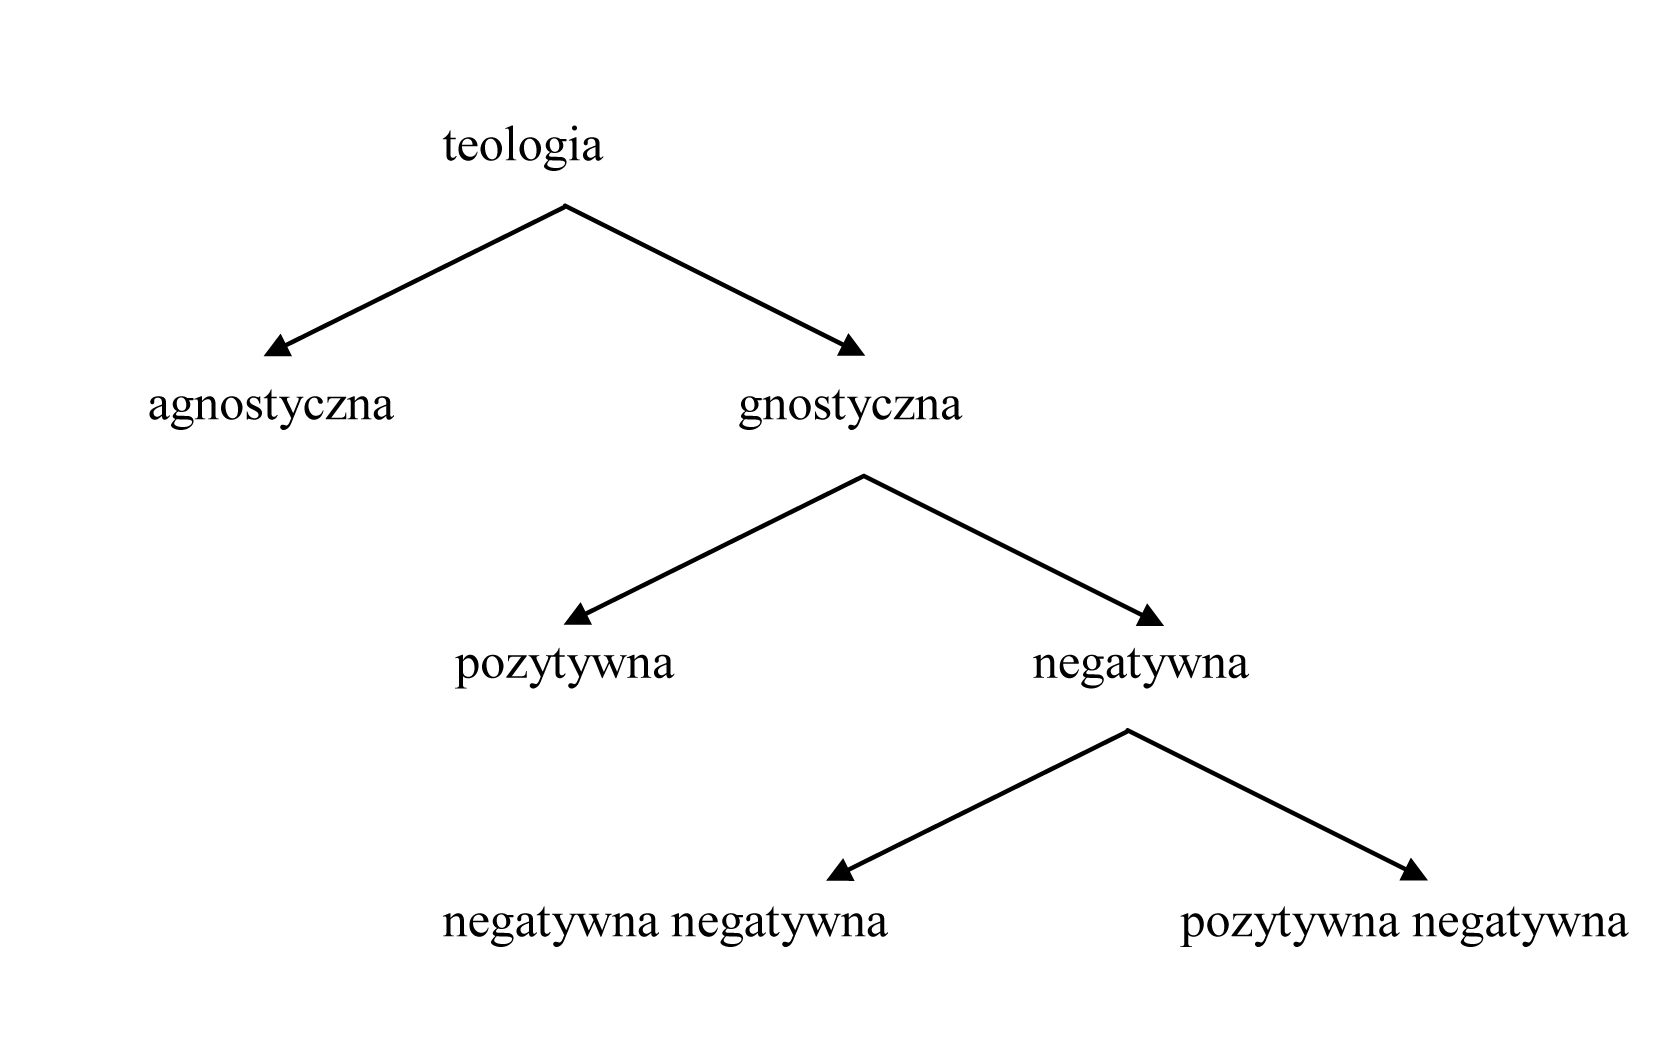
\includegraphics[width=1\linewidth]{typologia.jpg}
%\caption{Proponowana przez Rojka
%typologia interpretacji teologii apofatycznej.}
%}
%\end{figure}

%\begin{figure}[H]
%\begin{center}
% \begin{tikzpicture}[node distance=1cm]
%
%    \node (1) {teologia};
%    \node (21) [below=of 1, xshift=-2.5cm] {agnostyczna};
%    \node (22) [below=of 1, xshift=2.5cm] {gnostyczna};
%    \node (31b) [below=of 22, xshift=-2.5cm] {pozytywna};
%    \node (32b) [below=of 22, xshift=2.5cm] {negatywna};
%    \node (41) [below=of 32b, xshift=-2.5cm] {negatywna negatywna};
%    \node (42) [below=of 32b, xshift=2.5cm] {pozytywna negatywna};
%
%    \path[-] (1) edge (21);
%    \path[-] (1) edge (22);
%    \path[-] (22) edge (31b);
%    \path[-] (22) edge (32b);
%    \path[-] (32b) edge (41);
%    \path[-] (32b) edge (42);
%
%\end{tikzpicture}
%
%\caption[Typologia teologii apofatycznej według Rojka]{Proponowana przez Rojka
%typologia interpretacji teologii apofatycznej.}\label{roj-typ-rys}
%\end{center}
%\end{figure}

%Problemem, któremu Rojek poświęca nieco uwagi, lecz mimo wszystko
%postanawia go nie rozstrzygać, jest problem własności pozytywnych. Jest
%to problem poważny, ponieważ w świetle przedstawionej powyżej typologii
%różnica między teologią pozytywną i negatywną polega na orzekaniu o
%najwyższej istocie pozytywnych własności lub ich negacji. Jak
%zdefiniować zbiór takich własności? Rojek wymienia kryterium
%syntaktyczne, które miałoby polegać na ,,obecności negacji w
%predykacie''\footnote{Tamże, s. 221. }. Nie do końca wiadomo, jak
%rozumieć takie kryterium. Przypuszczam, że formalnie można zapisać tę
%propozycję w logice predykatów II-rzędu w następujący sposób:
%
%\begin{equation}
%    P(Q) {=}_{df} \forall x \neg \exists N (Q(x) \equiv \neg N(x)),
%\end{equation}
%gdzie $P(Q)$ oznacza ,,własność $Q$ jest pozytywna''. Jednakże Rojek
%natychmiast dodaje, że kryterium syntaktyczne nie może być uważane za
%wystarczające. Powołuje się tu na klasyczny przykład predykatu ,,jest
%ślepy'' -- nie zawiera on negacji, lecz odnosi się do braku i z tego
%powodu wydaje się być pozytywny. Trafniejszym argumentem wydaje się być
%powołanie na św. Tomasza, wedle którego własności tradycyjnie
%przypisywane bytowi absolutnemu, takie jak prostota, doskonałość czy
%jedność, są w istocie własnościami negatywnymi\footnote{św. Tomasz z
%Akwinu Teologiczna: I, 3, Summa contra Gentiles 11. }.
%
%Problem własności pozytywnych Rojek pozostawia nierozwiązany tłumacząc,
%że skupia się na formie teologii negatywnej, nie na jej treści. Dodaje
%jednak, że istnieje jeszcze jeden bardzo szczególny sposób ich
%rozumienia. Można je traktować, jako najwyższy sposób istnienia danej
%własności, czyli tzw. perfekcje. Najczęściej mówi się o takich
%perfekcjach, jak wszechwiedza -- najwyższy sposób wiedzy, czy też
%wszechmoc -- najwyższy stopień mocy. Są one istotnym elementem w
%ontologicznych dowodach istnienia Boga, które w historii były
%proponowane m.in. przez św. Anzelma, Kartezjusza, Leibniza, Gödla i
%Perzanowskiego. W tych argumentach Boga można uznać za podmiot
%wszelkich własności pozytywnych rozumianych jako perfekcje:
%
%\begin{equation}
%    G(x) \equiv \forall Q (P(Q) \to Q(x)).
%\end{equation}
%
%
%Definicję tę Rojek zaczerpnął od Perzanowskiego\footnote{J.
%Perzanowski, Ontological Arguments II: Cartesian and Leibnizian, [w:]
%red. H. Burkhardt, B. Smith, Handbook of Metaphysics and Ontology, t.
%2, PhilosophiaVerlag, München 1991,ss.~625–633. } i stanowi ona
%wzór kolejnych definicji Boga w proponowanych przez niego następnie
%interpretacjach teologii negatywnej. Warto wiec poświęcić jej nieco
%uwagi. Po pierwsze, jest ona zapisana w rachunku predykatów drugiego
%rzędu, gdyż zawiera warunek, że własności przypisywane Bogu muszą być
%pozytywne. Po drugie, Bóg formalizowany jest jako predykat (,,$x$ jest
%Bogiem'', ,,$x$ jest bogopodobny''), nie jako stała logiczna\footnote{Por.
%choćby M. Durrant, The ,,Meaning of ‘God’-I, Royal Institute of
%Philosophy Supplement,vol. 31 (1992), ss. 71-84. }, lub deskrypcja
%określona, co proponował Bocheński\footnote{J.M. Bocheński, dz. cyt.,
%s. 381. }. Po trzecie, powyższa definicja powstała na użytek
%formalizacji dowodów ontologicznych, które należą raczej do jakiejś
%formy teologii pozytywnej. Zawarte w niej $P(Q)$ czytamy jako ,,$Q$ jest
%własnością pozytywną'' w pewnym szczególnym sensie opisanym powyżej -- ,,$Q$
%jest perfekcją''. Rojek nie sugeruje jednak, że w teologii apofatycznej
%Pseudo-Dionizego zaprzecza się jedynie tego typu własnościom
%pozytywnym. Przeciwnie, pisze wprost, że zakres negowanych własności
%jest szerszy\footnote{P. Rojek, dz. cyt., s. 222. }. Po raz
%kolejny jednak odżegnuje się od określenia, o jakie konkretnie
%własności chodzi. Jest to, moim zdaniem, jeden z najsłabszych punktów
%jego propozycji. Wrócę do tego ponownie w dyskusji.


\section{Agnostyczna teologia negatywna}\label{roj-agnostycna}

Strategią pierwszej przedstawianej przez Rojka\index[names]{Rojek, Paweł} apofatycznej teorii Boga
jest przyjęcie \eqref{rojek-T4} jako tezy podstawowej i odrzucenie lub
modyfikacja pozostałych tez, za cenę zachowania spójności.
Jak już ujawniliśmy, celem tego typu doktryny jest podkreślenie znaczenia
boskiej transcendencji -- teoria ta głosi, że Bóg jest zasadniczo niewyrażalny
i~niepojmowalny. Takie rozumienie teologii negatywnej jest popularne wśród wielu
komentatorów -- także tych, którzy rozważają logiczno-językową strukturę
tej teorii\footnote{Wśród nich Rojek\index[names]{Rojek, Paweł} wymienia Jerome'a Gellmana\index[names]{Gellman, Jerome I.}, Johna J.
Jonesa\index[names]{Jones, John J.} oraz Paula Rorema\index[names]{Rorem, Paul}. Zob., odpowiednio, rozdz. \ref{sil-gell} oraz \ref{sil-dionizy}.}.

%W rozważaniach Gellmana teologia negatywna jest teorią, w której
%jakikolwiek predykat P języka ,,skończonych bytów'' nie może być
%przedziwie orzekany o Bogu. Jej główną tezą jest, że Bóg nie należy do
%zakresu żadnego z predykatów naszego języka. Jeśli mówimy na przykład,
%że Bóg nie jest mądry, mamy na myśli raczej negacją
%\textit{wykluczającą}, niż negację \textit{wyboru}. Naszym zamiarem
%jest wyłącznie stwierdzenie, że to nieprawda, że predykat P przysługuje
%Bogu, niekoniecznie sugerując, że można o nim orzec dopełnienie tego
%predykatu, czyli nie-P\footnote{J.I. Gellman, The Meta-Philosophy of
%Religious Language. ,,No\^us'', nr 11 (1971), s. 158. }. Według
%Gellmana, zdanie ,,Bóg jest potężny'' teolog negatywny zrozumie jako
%negację dopełnienia predykatu ,,jest potężny''. W innym kontekście
%oznaczałoby to przypisanie obiektowi, o którym mowa, tej właśnie
%własności. Jednakże w przypadku Boga negowanie dopełnienia predykatu P
%nie oznacza przypisywania mu P. Mówiąc ogólnie, zdania języka
%religijnego negują dopełnienia wszystkich wymienianych przez nie
%własności Boga, który jest poza zakresem wszystkich naszych predykatów.
%One, z kolei -- będąc predykatami języka skończonych bytów -- z
%konieczności muszą oznaczać niedoskonałe własności\footnote{Zob.
%Tamże. }.
%
%Według Jonesa, teologia negatywna Pseudo-Dionizego Areopagity jest w
%dużej mierze teologią krytyczną. Polemizuje ona z błędnym sposobem
%mówienia o Bogu -- takim, który traktuje Go jak byty, czyli rzeczy lub
%pojęcia\footnote{J.J. Jones, dz. cyt., s. 357. }. Fakt, że Bóg
%przekracza wszelki byt, nadaje również strukturę językowi dyskursu
%teologicznego. Nie idzie tylko o to, że przypisywanie Bogu
%jakichkolwiek przymiotów przysługujących bytom jest z gruntu błędne.
%Zwykle, gdy mówimy o rzeczach, twierdzenia i przeczenia sprzeciwiają
%się sobie. W wykładni Dionizego nie dzieje się tak w przypadku Boga.
%Bóg nie jest jednym z bytów, zatem język służący do opisu bytów nie
%jest dla Niego właściwy. W wypracowanym przez niego języku teologicznym
%twierdzenia i zaprzeczenia należą do odmiennych grup, tworząc odmienne
%sposoby mówienia o Bogu. Ponieważ funkcjonują one w odmienny sposób,
%nie należy ich ze sobą mieszać. Te pierwsze przedstawiają Boga jako
%przyczynę wszystkiego, te drugie wyrażają jego transcendencję. Oba
%sposoby mówienia można stosować naraz zarówno do opisu Boga, jak i
%opisu przedmiotów, jednakże w ten sposób nie zdołamy wyrazić
%unikalności Boga -- tego, że jest czymś odrębnym od wszystkich
%bytów\footnote{Zob. Tamże, s. 360. }. Możemy tego dokonać
%wyłącznie przez negację, która według Jonesa jest kluczowym punktem
%myśli Dionizego. Istotnym jest, że Jones wyraźnie odróżnia negację od
%zaprzeczenia.
%
%
%\begin{quote}
%        W przeciwieństwie do zaprzeczenia, negacja odnosi się do (nie)możliwości
%poznania i powiedzenia czegokolwiek o Bogu. Jest to, jeśli można tak
%powiedzieć, reguła drugiego rzędu posługiwania się nazwami pierwszego
%rzędu.\footnote{Tamże, s. 381. Większą część tego cytatu podaję za
%Rojkiem, dz. cyt., s. 222. }
%\end{quote}






%Najbardziej agnostyczną interpretację dionizyjskiej teologii negatywnej
%zaproponował Paul Rorem. Podkreśla on podobieństwo teologii
%Pseudo-Dionizego z późną filozofią neoplatońską. W obu tych doktrynach
%byty uporządkowane są względem pewnej hierarchii i w celu dotarcia do
%bytu absolutnego należy ,,wspiąć się'' po tej ,,drabinie'' bytów. By
%spotkać Boga należy wpierw zanegować nasze wrażenia i wyobrażenia i
%przekroczyć je, by dojść do ich pojęciowych znaczeń. Następnie
%zanegowane zostać powinny także owe znaczenia oraz wszelkie inne
%pojęcia umysłu, ponieważ przekroczenie naszej wiedzy prowadzi do
%niepoznawalnego, do cichego zjednoczenia z Bogiem. Innymi słowy, Rorem
%zwraca uwagę, że u Areopagity drogą do Boga jest zaprzeczenie
%wszystkich bytów. Dionizy jednak wielokrotnie stwierdza, że Bóg jest
%także ponad wszelkim zaprzeczeniem. Ostatecznie więc, należy zanegować
%także wszelkie negacje, nie pozostawając już żadnym pojęciem
%Boga\footnote{Por. P. Rorem, Pseudo-Dionysius. A Commentary on the
%Texts and an Introduction to Their Influence, Oxford University Press,
%Oxford -- New York 1993, ss. 210-211. }. Jak zauważa Rorem, Dionizy
%,,zaprzecza i wykracza poza wszystkie nasze pojęcia lub «pojęciowe»
%atrybuty Boga i kończy na odrzuceniu wszelkiego mówienia i myślenia,
%nawet negatywnego''\footnote{Tenże, przypis do Pseudo-Dionizy
%Areopagita, The Complete Work, tłum. C. Luibheid,. Paulist Press, New
%York 1987, s. 99. Cytuję za P. Rojek, dz. cyt. }.





Wynikiem agnostycznej
interpretacji teologii negatywnej nie jest zatem twierdzenie, że Bóg posiada
własności negatywne. Stosunek Boga do własności -- czy to pozytywnych, czy negatywnych -- jest tu irrelewantny lub raczej niemożliwy do określenia. Główną tezą tej doktryny jest właśnie twierdzenie, że Bóg jest niewyrażalny i~niepoznawalny. 
Zgodnie ze wskazaną w~ten sposób dwuznacznością tezy \eqref{rojek-T4},
Rojek\index[names]{Rojek, Paweł} wyróżnia dwie wersje tej teorii. Wedle pierwszej z nich, Bóg jest
niewyrażalny, nie sposób go wysłowić.
%Konsekwentnym rozwinięciem tej
%teorii jest stwierdzenie, że dyskurs religijny jest pozbawiony
%jakiegokolwiek znaczenia.
Wedle drugiej wersji, Bóg jest
niepoznawalny, nie można posiąść o nim wiedzy.
%I choć dyskurs religijny
%posiada w tej teorii jakieś znaczenie, może on opisać wyłącznie to,
%czego o Bogu nie wiemy. Rojek omawia obie wersje tej interpretacji.
A zatem poruszamy się tutaj na gruncie dobrze nam znanej teologii milczenia, choć po raz pierwszy wyraźnie zaznaczony zostaje
wątek związany z niepoznawalnością Boga. Jak przekonuję w kolejnej części pracy\footnote{Zob. rozdz. \ref{scep}.}, teorię Niepoznawalnego należy
uważać za odrębną interpretacje teologii negatywnej. Umieszczenie tego fragmentu analiz Rojka\index[names]{Rojek, Paweł} w niniejszym rozdziale posiada jednak dodatkowe motywacje.
Po pierwsze, model tej teorii jest dla Rojka\index[names]{Rojek, Paweł} inspiracją w~budowaniu logicznej ramy dla jego własnej interpretacji -- pozytywnej teologii negatywnej. Bez przedstawienia sposobu, w~jaki Rojek\index[names]{Rojek, Paweł} dochodzi do logicznej rekonstrukcji teorii Niepoznawalnego, sprawozdanie z jego oryginalnego modelu straciłoby na jasności.
Po drugie, w~apofatycznej doktrynie Pseudo-Dionizego Areopagity\index[names]{Pseudo-Dionizy Areopagita}, która jest źródłem tez \eqref{rojek-T1}-\eqref{rojek-T4}, będących podstawą wszystkich rozważanych w niniejszym rozdziale teorii Boga, różnica między jego niewysławialnością a niepoznawalnością nie jest wyraźnie zarysowana.
Po trzecie, dosyć nietypowa syntaktyka zaproponowana przez Rojka\index[names]{Rojek, Paweł} do formalizacji teorii Niepoznawalnego nie posiada jednoznacznie epistemicznej natury, a~jej filozoficzne motywacje i~charakterystyka zdradzają symptomy świadczące, że w~tym przypadku wciąż pozostajemy na gruncie teologii milczenia.
W~końcu, do tego samego wniosku prowadzą nas Rojka\index[names]{Rojek, Paweł} komentarze do modelu teorii Niepoznawalnego, według których niepoznawalność Boga polega na niemożliwości \textit{twierdzenia}, że posiada on pozytywne własności.




\subsubsection{Teoria Niewysławialnego}\label{rojek-bochenski}

Teorię Niewysławialnego Rojek\index[names]{Rojek, Paweł} charakteryzuje zgodnie z duchem prezentowanej w~niniejszej części pracy teologii milczenia. Poprawnie identyfikuje jej paradoksalny charakter mający swe źródła w~samozwrotności.
Do jej rekonstrukcji adaptuje metajęzykowe ujęcie zaczerpnięte od Bocheńskiego\index[names]{Bocheński, Józef Maria}. Z~tego względu podstawową dla tej interpretacji teologii negatywnej tezę \eqref{rojek-T4} oddaje za Bocheńskim\index[names]{Bocheński, Józef Maria} jako
\begin{flalign*}
&G(x) \equiv \forall \mathcal{L}\ N_w(x,\mathcal{L}).&\tag{MNT''}\label{rojek-MNTbis}
\end{flalign*}

Rojek\index[names]{Rojek, Paweł} wydaje się być usatysfakcjonowany ustaleniami Bocheńskiego\index[names]{Bocheński, Józef Maria} i przekonany, że ujęcie teologii milczenia w postaci \ref{rojek-MNTbis} ratuje tę teorię przed sprzecznościami\footnote{Jak pokazałem w poprzednim rozdziale (rozdz. \ref{sil-boch-dyskusja}), można mieć co do tego wątpliwości.}.
Powyższą formułę wraz dodatkowymi uwagami głoszącymi, że mamy tu do czynienia z~wypowiedzią metajęzykową, nazywa ,,modelem'' teorii Niewysławialnego. Przyjmuje też w pełni Bocheńskiego\index[names]{Bocheński, Józef Maria} argumenty przeciwko teorii Niewysławialnego -- fakt, że nie możemy przypisać Bogu żadnej własności przedmiotowo-językowej sprawia, że teoria ta jest niezgodna z faktycznym dyskursem religijnym i religijną \textit{praxis}, a~więc dyskwalifikuje ją jako poprawną teorię Boga. Ze względu na jej uwikłanie w~swoje ,,zewnętrzne'' paradoksy należy ją odrzucić.



%Podobnie argumentuje John Hick, który uważa, że nie ma sensu
%
%
%\begin{quote}
%mówić o X, że żadne nasze pojęcie się do niego nie stosuje. Jest bowiem
%w oczywisty sposób niemożliwe odnosić się do czegoś, co nie posiada
%nawet własności 'bycia możliwym przedmiotem
%odniesienia.\footnote{J. Hick, An Interpretation of Religion. Human
%Responses to the Transcendent, Yale University Press, New Haven –
%Londyn 1989, s. 239. Cytuję za P. Sikora, Logos Niepojęty, Wydawnictwo
%Universitas, Kraków 2010, s. 118. }
%\end{quote}
%
%
%Dodaje on także, że określenie
%
%\begin{quote}
%,,taki, że nasze pojęcia się do niego nie stosują'' nie może,
%jeśli chcemy uniknąć paradoksu, odnosić się do własności, którą
%opisuje.\footnote{Tamże. }
%\end{quote}
%
%Przeciwko takiemu przedstawianiu teorii Niewysławialnego występuje Józef
%Maria Bocheński. Twierdzi on, że da się ją uratować od sprzeczności,
%lecz nawet mimo tego, nie odpowiada ona potrzebom dyskursu
%religijnego\footnote{Zob. J.M. Bocheński, dz. cyt., ss. 353-356.
%}. Bocheński uważa, że jeśli przestrzega się pewnych obowiązujących w
%logice konwencji, zarzut sprzeczności stawiany teorii Niewysławialnego
%przestanie obowiązywać. Należałoby wpierw dowieść, że danym układzie
%odniesienia teoria ta prowadzi do sprzeczności, tymczasem nikt takiego
%dowodu nie przedstawił. Według Bocheńskiego sytuacja przedstawia się
%zupełnie przeciwnie -- nietrudno wykazać, że teoria Niewysławialnego
%jest spójna. Poniżej przedstawię jego argumentację.
%
%Załóżmy, że dwuargumentowy predykat  $Nw(x,l)$ oznacza ,,$x$ jest
%niewyrażalne w języku $l$''.
%
%Zapiszmy teraz formułę zawierającą ten predykat
%
%\begin{equation}
%    \exists x \exists l Nw(x, l)
%\end{equation}
%
%
%Wydaje się, że nie tylko można ją wypowiedzieć nie popadając w
%sprzeczność, lecz także jest ona prawdziwa, nietrudno znaleźć taki
%obiekt $x$ i taki język $l$, które spełniałyby zapisany wyżej warunek.
%(Bocheński podaje przykład krowy i języka szachów: nie da się opisać
%krowy w języku szachów).
%
%Możemy powyższy przykład uogólnić i sformułować metajęzykową definicję
%Boga o następującej postaci:
%
%\begin{equation}\tag{G2}
%    G(x) \equiv \forall l Nw(x, l)\footnote{Definicję podaję za
%Rojkiem, różni się ona od zapisu Bocheńskiego tym, że u tego ostatniego
%,,Bóg'' zapisany został jako stała logiczna: $\forall l Nw(a, l)$.}
%\end{equation}
%
%
%
%Na pierwszy rzut oka, wydaje się, ze ta formuła jest bardziej
%problematyczna -- twierdzenie, że $x$ jest niewysłowione w żadnym języku
%zdaje się prowadzić do sprzeczności. Można jednak uniknąć tego
%problemu, stosując zwykłe konwencje wykorzystywane do pozbywania się
%antynomii semantycznych. Należy założyć, że żadne zdanie traktujące o
%pewnej klasie języków, nie jest formułowane w żadnym z tych języków.
%Aby było pozbawione sprzeczności musi zostać sformułowane w innym
%języku, czyli odpowiednim metajęzyku. Możemy więc założyć, że klasa
%języków wspominana w (G2) jest klasą języków przedmiotowych. W takim
%wypadku (G2) jest zdaniem metajęzyka pierwszego stopnia. Po takim
%zabiegu, sformułowana definicja jest znacząca i pozbawiona
%sprzeczności. Nie ma bowiem niespójności w twierdzeniu, że coś nie daje
%się wysłowić w jakimś języku, lub nawet w klasie języków, o ile
%twierdzenie to jest w języku nienależącym do tej klasy. Według
%Bocheńskiego, przy takim założeniu, standardowym z punktu widzenia
%logiki ogólnej, teoria Niewysławialnego pozostaje znacząca i spójna a
%zarzut sprzeczności zostaje oddalony.
%
%Bocheński odrzuca jednak teorię Niewysławialnego z co najmniej dwóch
%powodów. Po pierwsze, na mocy (G2) nie można przypisać Bogu
%jakiekolwiek własności językowo przedmiotowej. Jedyną własnością, jaką
%możemy mu przypisać, jest metajęzykowa własność bycia niewysłowionym w
%żadnym z języków przedmiotowych. W takim wypadku wierny, nie mógłby
%akceptować żadnego zdania dyskursu religijnego, które przypisałoby Bogu
%jakąkolwiek własność-przedmiotowo-językową. Wydaje się to niespójne z
%faktycznym dyskursem religijnym. Po drugie, niemożliwe byłoby oddawanie
%czci obiektowi, o którym wiemy tylko i wyłącznie, że nie można o nim
%nic powiedzieć. Jeśli wierny miałby czcić obiekt pozbawiony własności
%przedmiotowo-językowych, równie dobrze tym obiektem mógłby nie być Bóg
%a szatan\footnote{Por. J.M. Bocheński, dz. cyt., ss. 354-356. }.

%Rojek dodaje do tego podobny argument, jednakże umieszczony w kontekście
%teologii negatywnej. Mianowicie, jeśli teoria Niewysławialnego ma być
%właściwą interpretacją teologii negatywnej, można poddać w wątpliwość
%zasadność jednoczesnego utrzymywania tez \eqref{rojek-T1}-\eqref{rojek-T3}. Jeśli Bóg jest
%niewyrażalny, cały język religijny jest pozbawiony znaczenia, nie
%możemy więc ani sensownie potwierdzić, ani zaprzeczyć żadnym z Jego
%własności. Dla Rojka jest to wskazówka, by \eqref{rojek-T4} nie interpretować
%semantycznie, lecz epistemologicznie lub nawet
%ontologicznie\footnote{Zob. P. Rojek, dz. cyt., s. 223.}. W ten sposób przechodzi od
%teorii Niewysławialnego do agnostycznej teorii Niepoznawalnego.

Rojek\index[names]{Rojek, Paweł} dodaje do tego argument sformułowany w kontekście
swoich analiz. Mianowicie, jeśli teoria Niewysławialnego ma być
właściwą interpretacją teologii negatywnej, należy podać w wątpliwość
zasadność utrzymywania tez \eqref{rojek-T1}-\eqref{rojek-T3}. Jeśli Bóg jest
niewyrażalny, cały język religijny jest pozbawiony znaczenia, nie
możemy więc ani sensownie potwierdzić, ani zaprzeczyć żadnym z jego
własności. Krótko mówiąc, teoria Niewysławialnego zdaje się nie dawać żadnych szans na
akceptację którejkolwiek z wyabstrahowanych tez teologii apofatycznej poza \eqref{rojek-T4}.
Dla Rojka\index[names]{Rojek, Paweł} jest to wskazówka, by nie interpretować tej tezy
semantycznie, lecz epistemologicznie lub nawet
ontologicznie\footnote{Zob. P. Rojek, \textit{Logika teologii negatywnej}, dz. cyt., s. 223.}. W ten sposób przechodzi od
teorii Niewysławialnego do agnostycznej teorii Niepoznawalnego.


\subsubsection{Agnostyczna teoria Niepoznawalnego}

Według Rojka\index[names]{Rojek, Paweł} teoria Niepoznawalnego jest lepszym modelem teologii apofatycznej,
ponieważ nie tylko przyjmuje \eqref{rojek-T4} za twierdzenie podstawowe, lecz także
umożliwia pewną interpretację tez \eqref{rojek-T2} oraz \eqref{rojek-T3}. By to pokazać,
wprowadza pojęcie nieokreśloności oraz definiuje nowe, odmienne od
klasycznego pojęcie negacji. W tym celu wykorzystuje on logiczną teorię
nieokreśloności, którą na potrzeby modelowania (w~filozofii) nauki rozwinął
rosyjski logik Aleksander Zinowjew\index[names]{Zinowjew, Aleksander}\index[names]{Zinowjew, Aleksander}\footnote{A.A. Zinov'ev, \textit{Foundations
of the Logical Theory...}, dz. cyt. Zob. także tenże,
\textit{Logika nauki}, dz. cyt. }.

Filozoficzną motywacją logiki Zinowjewa\index[names]{Zinowjew, Aleksander} są  pewne ,,nieklasyczne'' przypadki
spotykane w teoriach i wynikach naukowych oraz ich interpretacjach, w których zniesione zostaje
prawo wyłączonego środka. Takie przypadki polegają na dopuszczeniu
możliwości istnienia obiektów, co do których nie da się ustalić, czy
posiadają one jakąś własność $Q$, czy też posiadają własność
$\neg Q$. Można do nich zaliczyć na przykład rozważaną
w~mechanice kwantowej cząstkę elementarną, której parametry -- zgodnie z
zasadą nieoznaczoności~-- nie mogą zostać ustalone\footnote{Interesujące może okazać się zbadanie związków pewnych rozwiązań wypracowanych w~ramach
teologii negatywnej
oraz filozofii mechaniki kwantowej.
Tym, którzy podają w wątpliwość teoretyczną wartość teologii negatywnej,
istnienie innych obszarów, w których możliwości ludzkiego języka i pojęć zdają się być niewystarczające, może dostarczyć argumentu
na rzecz wiarygodności tej doktryny jako teologicznej teorii tego, nie niewysławialne i niepojmowalne.
},
twierdzenie, które
na gruncie danego rachunku logicznego nie może zostać ani dowiedzione,
ani obalone, albo po prostu obiekt zmieniający się w~czasie. Na
potrzeby takich przypadków Zinowjew\index[names]{Zinowjew, Aleksander} nad logiką klasyczną wprowadza nowy funktor nieokreśloności i
oznacza go symbolem $?$\footnote{Dla utrzymania spójności zapisu, formuły teorii
nieokreśloności Zinowjewa\index[names]{Zinowjew, Aleksander} przedstawiam w~nieco zmodyfikowanej notacji zaproponowanej przez
Rojka\index[names]{Rojek, Paweł}.}. Niech zapis $?Q(x)$ oznacza ,,nie można
ustalić, czy $x$ ma $Q$, czy $x$ ma nie-$Q(x)$'', co można czytać także jako ,,$x$ ma w sposób
nieokreślony $Q$''. W~teorii Niepoznawalnego Bóg uznawany jest za
obiekt, którego nie da się poznać. Rojek\index[names]{Rojek, Paweł} proponuje, by za pomocą powyższego funktora nieokreśloności z logiki Zinowjewa\index[names]{Zinowjew, Aleksander}
podać nową definicję Boga jako obiektu, który wszystkie pozytywne
własności posiada w~sposób nieokreślony.
\begin{flalign*}
&G(x) \equiv \forall Q (P(Q) \to ?Q(x)).&\tag{ZNT}\label{rojek-ZNT}
\end{flalign*}
%\begin{equation}\tag{G3}
%   G(x) \equiv \forall Q (P(Q) \to ?Q(x)).
%\end{equation}

%
%
%Formule tej należy poświęcić nieco uwagi. Po pierwsze, w odróżnieniu od
%\ref{sil-boch-MNT} powyższa definicja nie jest wyrażona w metajęzyku, lecz w języku
%przedmiotowym. Po drugie, co istotniejsze, by uniknąć kłopotów z
%formalizowaniem Boga przy użyciu predykatu $G(x)$, należy ją ograniczyć.
%Do tej definicji trzeba dołożyć dodatkowe założenie, o postaci:
%
%\begin{equation}
%    \neg P(G)
%\end{equation}
%
%
%Innymi słowy, należy założyć, że predykat ,,jest Bogiem'' (lub ,,jest
%bogopodobny'') nie należy do zbioru predykatów pozytywnych. W
%przedziwnym bowiem razie, wpadlibyśmy w błędne koło i o niczym nie
%można byłoby określić, że jest Bogiem.

Jak twierdzi Rojek\index[names]{Rojek, Paweł}, wykorzystując ten formalizm do modelowania teorii
Niepoznawalnego, można -- w pewnym szczególnym sensie -- zaprzeczyć, że
Bóg posiada wszystkie własności pozytywne.
%Oczywiście, nie idzie tutaj
%o stwierdzenie, że o Bogu można na orzec jakiekolwiek
%$\neg Q$, przy założeniu, że $Q$ jest własnością pozytywną.
%Taki przypadek jest niezgodny zasadą \ref{rojek-ZNT}.
Idzie o to, że po
wprowadzeniu funktora nieokreśloności $?$, zdanie
,,nieprawda, że $x$ jest
$Q$''\footnote{Rojek mówi o wyrażeniu ,,$x$ jest nie-$Q$'', moim zdaniem
błędnie. W ogóle w przedstawieniu teorii Niepoznawalnego w szacie logiki nieokreśloności Zinowjewa\index[names]{Zinowjew, Aleksander} odnaleźć można dużo niezgrabności. Por. P.~Rojek, \textit{Logika teologii negatywnej}, dz. cyt., s.~223. Kładę to jednak na karb nietypowej notacji stosowanej przez radzieckiego logika, którą Rojek\index[names]{Rojek, Paweł} próbuje przeredagować według bardziej współczesnych standardów.} staje się dwuznaczne. Może ono przyjąć jedno
z dwóch znaczeń: albo ,,$x$ jest nie-$Q$'', albo ,,nie można stwierdzić, czy $x$~jest~$Q$''. W nomenklaturze Rojka\index[names]{Rojek, Paweł}, w pierwszym przypadku w~zdaniu pojawia
się negacja w~znaczeniu \textit{de dicto}, o~drugim znaczeniu natomiast
można mówić, że zawiera ono negację \textit{de re}. Nieco inne
nazewnictwo wprowadził Zinowjew\index[names]{Zinowjew, Aleksander}, który pierwszy rodzaj negacji nazwał
negacją zewnętrzną -- odnosi się ona bowiem do całego negowanego w~ten
sposób zdania, drugą negację nazwał
negacją wewnętrzną -- dotyczy ona bowiem wyłącznie predykatu\footnote{Konkretnie: operatora predykatywności.
Notacja zaproponowana przez Rojka\index[names]{Rojek, Paweł} pozbawiona jest już symbolu takiego operatora.}.

Przyjmijmy teraz dwa różne symbole, w celu odróżnienia odmiennych pojęć
negacji. Niech $\neg$ oznacza negację zewnętrzną,
natomiast symbol $\sim$ negację wewnętrzną. Przy
takiej notacji, formułę ${\sim}Q(x)$ czytamy jako ,,$x$ jest
nie-$Q$'', lub  inaczej: ,,$x$ ma własność nie-$Q$''\footnote{U Rojka\index[names]{Rojek, Paweł}: ,,$x$ ma
własność $\neg Q$''. }, natomiast formuła
$\neg Q(x)$\footnote{Rojek używa tych symboli na odwrót, to jest $\neg$ stosuje na oznaczenie negacji
wewnętrznej, a~$\sim$~używa do oddania negacji zewnętrznej. Dodatkowo formułę negowaną za pomocą
funktora negacji zewnętrznej opatruje w dodatkowe nawiasy po to, by
podkreślić odmienny, ,,zewnętrzny'' charakter tego rodzaju negacji.
Uznaję ten zabieg za redundantny i niekonieczny. Notacja Rojka\index[names]{Rojek, Paweł} jest odmienna od
stosowanej oryginalnie przez Zinowjewa\index[names]{Zinowjew, Aleksander}.} oznacza ,,nieprawda, że $x$~jest $Q$'', lub ,,nie twierdzi się, że
$x$~ma własność $Q$''. Poniższe aksjomaty definiują relacje, jakie zachodzą
pomiędzy funktorem nieokreśloności a funktorami negacji wewnętrznej i~zewnętrznej\footnote{Aksjomaty podaję za Rojkiem\index[names]{Rojek, Paweł}, bez żadnej kwantyfikacji i konsekwentnie trzymam się tej konwencji.}:
\begin{flalign*}
&\neg Q(x) \equiv {\sim} Q(x)\ \lor\ ?Q(x),&\tag{Z\textsubscript{1}}\label{rojek-zin1}\\
&\neg {\sim} Q(x) \equiv Q(x)\ \lor\ ?Q(x),&\tag{Z\textsubscript{2}}\label{rojek-zin2}\\
&\neg ?Q(x) \equiv Q(x)\ \lor\ {\sim} Q(x)  .&\tag{Z\textsubscript{3}}\label{rojek-zin3}
\end{flalign*}
%\begin{equation}\tag{Z1}
%\neg  Q(x) \equiv ?Q(x) \lor {\sim} Q(x),
%\end{equation}
%\begin{equation}\tag{Z2}
%\neg {\sim} Q(x) \equiv Q(x)\ \lor\ ?Q(x),
%\end{equation}
%\begin{equation}\tag{Z3}
%\sim ?Q(x) \equiv Q(x) \lor {\sim} Q(x).
%\end{equation}
Z \eqref{rojek-zin3} oraz prawa De Morgana\index[names]{De Morgan, Augustus} bezpośrednio wynika:
\begin{flalign}
& ?Q(x)\ \equiv\ \neg  Q(x)\ \land\ \neg {\sim} Q(x). &\label{rojek-zin4}
\end{flalign}
%\begin{equation}
%   \vdash \quad ?Q(x)\ \equiv\ \neg  Q(x)\ \land\ \neg {\sim} Q(x).
%\end{equation}
 



Gdybyśmy chcieli dokonać kolapsu z powrotem do logiki klasycznej,
musielibyśmy założyć, że (dla każdego $x$, dla dowolnego $Q$) zachodzi $\neg ? Q(x)$. Prawdziwe jest bowiem twierdzenie

\begin{flalign}
&  \neg ?Q(x)\ \to \big({\sim} Q(x) \equiv \neg Q(x)\big).&
\end{flalign}
Przy założeniu, że nie istnieją przypadki nieokreśloności, negacje \textit{de re} i \textit{de
dicto} stają się tożsame.
Jednakże, jeśli
chcemy opisać wspomniane wyżej przypadki nieklasyczne, w~których
posiadanie lub nieposiadanie danej własności przez jakiś obiekt
nie może zostać określone, musimy zgodzić się na obecność dwóch
różnych, nierównoważnych pojęć negacji w systemie. Z tego powodu
poniższa formuła nie jest wyprowadzalna w ramach prezentowanego tu systemu:
\begin{flalign}
& \nvdash  \neg  Q(x) \to  {\sim} Q(x). &
\end{flalign}
%
%\begin{equation}
%    \nvdash \quad \neg  Q(x) \to  {\sim} Q(x).
%\end{equation}
Dzieje się tak, ponieważ $\neg Q(x)$ pociąga za sobą ${\sim} Q(x)$ lub
$?Q(x)$. Analogicznie, w~prezentowanym tu rachunku nie zachodzi
następująca wersja prawa podwójnej negacji
\begin{flalign}
& \nvdash   \neg  {\sim} Q(x) \to  Q(x), &
\end{flalign}
%
%
%\begin{equation}
%   \nvdash   \neg  ({\sim} Q(\textit{x})) \to  Q(\textit{x}),
%\end{equation}
ponieważ $\neg {\sim} Q(x)$ implikuje $Q(x)$ lub $?Q(x)$. Prawdziwe są
natomiast następujące formuły:
\begin{flalign}
&   {\sim} Q(x) \to  \neg  Q(x), &\\
&   Q(x) \to  \neg  {\sim} Q(x). &
\end{flalign}


%\begin{equation}
%    \vdash \quad {\sim} Q(x) \to  \neg  Q(x),
%\end{equation}
%\begin{equation}
%    \vdash \quad Q(x) \to  \neg  {\sim} Q(x).
%\end{equation}






Należy zauważyć, że dla negacji wewnętrznej nie można mówić
o ,,nieklasycznym'' prawie wyłączonego środka
\begin{flalign}
& \nvdash  Q(x) \lor {\sim} Q(x), &
\end{flalign}
%
%\begin{equation}
%     \nvdash \quad Q(x) \lor {\sim} Q(x),
%\end{equation}
ponieważ istnieje dodatkowa, trzecia możliwość -- $?Q(x)$. Do grona tez tego
rachunku należy zatem następująca formuła:
\begin{flalign}
&    Q(x) \lor  {\sim} Q(x)\ \lor\  ?Q(x). &
\end{flalign}
%\begin{equation}
%    \vdash \quad Q(x) \lor  {\sim} Q(x) \lor  ?Q(x)
%\end{equation}
Prawo wyłączonego środka obowiązuje natomiast dla negacji \textit{de
dicto}:
\begin{flalign}
&    Q(x) \lor  \neg  Q(x), &\\
&    {\sim} Q(x) \lor  \neg  {\sim} Q(x), &\\
&    ?Q(x) \lor  \neg  ?Q(x). &
\end{flalign}
%\begin{equation}
%    \vdash \quad Q(x) \lor  \neg  Q(x),
%\end{equation}
%\begin{equation}
%    \vdash \quad {\sim} Q(x) \lor  \neg  {\sim} Q(x),
%\end{equation}
%\begin{equation}
%\vdash \quad ?Q(x) \lor  \neg  ?Q(x).
%\end{equation}

Niewątpliwym wkładem Rojka\index[names]{Rojek, Paweł} jest spostrzeżenie, że rachunek Zinowjewa\index[names]{Zinowjew, Aleksander} stworzony pierwotnie na potrzeby
logicznej rekonstrukcji  pewnych teorii naukowych, w~ramach których naruszona zostaje reguła \textit{tertium non datur}, może okazać się przydatny także do modelowania
omawianej w tym paragrafie interpretacji teologii apofatycznej. Dzięki
 własnościom tego rachunku, można przedstawić w sposób niesprzeczny już trzy spośród
tez wypreparowanych z pism Pseudo-Dionizego Areopagity\index[names]{Pseudo-Dionizy Areopagita}. Rekonstrukcją
tezy \eqref{rojek-T4} w~obrębie tej interpretacji i w terminach rachunku Zinowjewa\index[names]{Zinowjew, Aleksander} jest definicja Boga podana przez \ref{rojek-ZNT}.
Z tejże formuły, na podstawie praw logiki Zinowjewa\index[names]{Zinowjew, Aleksander} nietrudno już wyprowadzić dwie kolejne tezy doktryny Dionizego\index[names]{Pseudo-Dionizy Areopagita}.

Negację, o której mowa
w \eqref{rojek-T2}, można traktować jako negację \textit{de dicto}, ponieważ
zgodnie z teorią Niepoznawalnego, nie możemy stwierdzić, czy
Bóg posiada jakieś własności\footnote{Ten fragment analiz Rojka\index[names]{Rojek, Paweł} jest trochę naciągany. Związane jest to z~narzuceniem specyficznej interpretacji na funktor ,,zwykłej'', zewnętrznej negacji \textit{de dicto} jako ,,nie można stwierdzić, że'', podczas gdy taka interpretacja prędzej przysługiwałaby funktorowi nieokreśloności. Jednakże biorę to rozumienie za dobrą monetę, a~słabe punkty analiz Rojka\index[names]{Rojek, Paweł} wskażę w innych miejscach.}. W takim podejściu, \eqref{rojek-T2} stwierdza, że o
Bogu można orzec zewnętrzne negacje wszystkich własności pozytywnych. A
zatem, w języku tego rachunku należałoby to zapisać w następujący sposób:
\begin{flalign}
&    G(x) \to  (\forall Q (P(Q) \to  \neg Q(x)). &\tag{T2'}\label{rojek-T2prim}
\end{flalign}
%
%
%\begin{equation}
%    G(x) \to  (\forall Q (P(Q) \to  \neg Q(x)).
%\end{equation}
%
%
%
Co więcej, powyższa formuła jest bezpośrednią konsekwencją definicji
\ref{rojek-ZNT} i (\ref{rojek-zin4}). Ponieważ negacja
\textit{de dicto} jest różna od negacji \textit{de re}, nie możemy
jednocześnie twierdzić, że Bóg posiada (wewnętrzną) negację wszystkich
pozytywnych własności, czyli że można o~nim orzekać każde nie-$Q$, o ile
$Q$ jest pozytywne. Z~obu tych formuł wynika
także
\begin{flalign}
&    G(x) \to  (\forall Q (P(Q) \to
\neg {\sim} Q(x)), &\tag{T3'}\label{rojek-T3prim}
\end{flalign}
%
%\begin{equation}
%    G(x) \to  (\forall Q (P(Q) \to
%\neg {\sim} Q(x)),
%\end{equation}
%
%
którą Rojek\index[names]{Rojek, Paweł} uważa  za zrekonstruowaną w ramach syntaksy Zinowjewa\index[names]{Zinowjew, Aleksander} tezę \eqref{rojek-T3}.
Formuła ta zawiera
podwójne przeczenie, jednakże pierwsza negacja ma charakter \textit{de
dicto}, natomiast druga jest negacją \textit{de re}. Brzmieniem tej
formuły jest ,,Nieprawda, że Bóg posiada wszystkie wewnętrzne negacje
pozytywnych własności''.

W takim wypadku, wszystkie stwierdzenia Dionizego\index[names]{Pseudo-Dionizy Areopagita} o tym, że Bóg nie jest
ani $Q$, ani nie-$Q$, na przykład że nie jest on ,,ani wielkością, ani
małością, ani równością, ani nierównością, ani podobieństwem, ani
niepodobieństwem'', ,,nie jest też niczym z niebytu ani czymś z
bytu''\footnote{Pseudo-Dionizy Areopagita, \textit{Teologia mistyczna}, dz.
cyt., rozdział V. } itp.,  można niesprzecznie interpretować w
ramach powyższej rekonstrukcji. Podobnie wypowiedzi Areopagity\index[names]{Pseudo-Dionizy Areopagita} o
tym, że Bóg jest ,,ponad wszelkim twierdzeniem i~ponad wszelkim
zaprzeczeniem''\footnote{Tamże.} można ująć w ramach
prezentowanego rachunku, jako koniunkcję warunków zawartych już
w~formułach \eqref{rojek-T2prim} i \eqref{rojek-T3prim}.
\begin{flalign}
&    G(x) \to  (\forall Q (P(Q) \to  \neg  Q(x) \land
\neg {\sim} Q(x)). &
\end{flalign}

%\begin{equation}
%    G(x) \to  (\forall Q (P(Q) \to  \neg  Q(x) \land
%\neg {\sim} Q(x)).
%\end{equation}



%Jak zauważa Rojek, istnieje wyjątek od konsekwentnego stosowania tej
%interpretacji. Nie można w ten sposób formalizować  twierdzeń, że Bóg
%nie jest ani poznawalny ani niepoznawalny, ani określony, ani
%nieokreślony. Taka treść predykatu $Q$ naraziłaby bowiem tę interpretację
%na sprzeczność. Jednakże wydaje się, że żadne z dzieł Dionizego nie
%zawiera podobnych sformułowań\footnote{Także Jones zauważa, że teza o
%niepoznawalności Boga ma wyjątkowy charakter w pismach Dionizego i
%nigdy nie występuje w podobnych parach. Zob. J.J. Jones, dz. cyt., s.
%358. }.


Rojek\index[names]{Rojek, Paweł} jest przekonany, że powyższe analizy chronią agnostyczną teologię negatywną przed
sprzecznościami, a~największą ich wadą jest to, że nie obejmują wszystkich tez wypreparowanych z pism Areopagity\index[names]{Pseudo-Dionizy Areopagita}.
Na tym gruncie teoria Niepoznawalnego wydaje się lepszą
interpretacją teologii negatywnej -- można w jej ramach
przyjąć aż trzy z apofatycznych tez. Teoria
Niewysławialnego ustępuje w tym zestawieniu  i obejmuje tylko jedną
tezę dionizyjskiej doktryny. Obie jednak zawodzą w interpretacji \eqref{rojek-T1}.
Teza ta nie znajduje swojego miejsca w agnostycznych 
interpretacjach, bowiem -- skoro Bóg jest niepoznawalny -- nie można o nim
nic sensownie stwierdzić.
Do tej uwagi Rojek\index[names]{Rojek, Paweł} dokłada argumenty Bocheńskiego przeciw teorii Niewysławialnego -- tym razem stosując je do obu interpretacji w ramach agnostycznej teologii negatywnej.
Są one zasadniczo niespójne z faktycznym dyskursem
i praktyką religijną. Zgodnie z ich duchem, wierny nie mógłby
akceptować żadnych zdań dyskursu religijnego, które przypisują Bogu
jakieś własności. Tymczasem każdy dyskurs religijny zawiera
przynajmniej kilka takich zdań. Poza tym, gdyby o Bogu nie można było
orzekać żadnych własności, nie mógłby on być przedmiotem wiary i~czci\footnote{
Zob. J.M. Bocheński, \textit{Logika religii}, dz. cyt., ss. 355-356, a~także rozdz. \ref{sil-boch-nonsens}.}.




\section{Negatywna teologia negatywna}

Wad tych pozbawiona jest druga interpretacja teologii negatywnej, którą
Rojek\index[names]{Rojek, Paweł} nazywa negatywną teologią negatywną. Jej punktem wyjścia jest
teza \eqref{rojek-T2}. Na gruncie tej interpretacji nie twierdzi się, że
dyskurs religijny pozbawiony jest znaczenia, ani że Bóg jest
niepoznawalny. Uważa się natomiast, że o przedmiocie religijnym można
orzekać wyłącznie negatywne własności. Nie jest więc tak, że nic nie
wiemy o Bogu -- wiemy, że nie posiada on pozytywnych własności.
%Należy
%przyznać, że jest to dość popularna interpretacja teologii
%apofatycznej. Na przykład, do właśnie w taki sposób rozumianej teologii
%negatywnej odnosił się Józef Maria Bocheński w dziele \textit{Logika
%religii}.

%W analizie Rojka, negację obecną w \eqref{rojek-T2}
%należy traktować w~zwykły, klasyczny sposób. Zatem \eqref{rojek-T1} oraz \eqref{rojek-T3} muszą zostać natychmiast odrzucone, jako niespójne z tezą przyjętą tu za podstawową.
Z drugiej strony, wedle tej wersji teologii negatywnej, wszystko, co możemy orzec o~Bogu,
posiada ściśle negatywny charakter. Na tym ma polegać boska transcendencja.
Choć taka teoria zatraca swój samozwrotny charakter (obecny w jakimś
stopniu w agnostycznej teologii negatywnej), w jej analizach nietrudno wskazać innego rodziaju sprzeczności. W~obrębie tej interpretacji Bóg
wciąż pozostaje w jakimś
sensie niepoznawalny -- jedyne, co o Nim wiemy to jaki nie jest. Można
więc pokusić się także na próbę uwzględnienia tezy \eqref{rojek-T4} w ramach modelu tej teorii.

Rojek\index[names]{Rojek, Paweł} twierdzi, że w tym modelu teologii negatywnej właściwą definicją
Boga jest formalizacja tezy \eqref{rojek-T2} w obrębie klasycznego rachunku
predykatów drugiego rzędu.
Skoro mamy do czynienia z~klasyczną negacją, \eqref{rojek-T1} oraz \eqref{rojek-T3} muszą zostać natychmiast odrzucone jako niespójne z tezą przyjętą tu za podstawową.
Bóg -- analogicznie do poprzednich definicji –
opisany jest jako obiekt, o którym można orzekać negacje wszystkich
pozytywnych własności:
\begin{flalign}
&    G(x) \equiv  \forall Q (P(Q) \to
\neg Q(x)). &\tag{NNT''}\label{rojek-NNTbis}
\end{flalign}

%\begin{equation}\label{G4}\tag{G4}
%    G(x) \equiv  \forall Q (P(Q) \to
%\neg Q(x)).
%\end{equation}


Powyższa definicja jest trawestacją zasady \ref{sil-boch-NNT} proponowanej przez Bocheńskiego\index[names]{Bocheński, Józef Maria}. Zatem wszystkie krytyczne uwagi formułowane w poprzednim rozdziale\footnote{Zob. rozdz. \ref{sil-boch-dyskusja}.} będą trafne także w przypadku omawianych tu rozważań Rojka\index[names]{Rojek, Paweł}. Zdaje się on być świadomy problemów nękających tę teorię Boga. Podaje zresztą zestaw ograniczeń, które należy do niej wprowadzić, by w proponowany model nie
wkradła się żadna sprzeczność. Najważniejsze ograniczenia dotyczą zbioru
pozytywnych własności. Jak wspominałem wcześniej, Rojek\index[names]{Rojek, Paweł} nie podaje
żadnej definicji, ani kryterium wyróżniania takich własności. Czyni jedynie na ten temat kilka uwag,
które w większym bądź mniejszym stopniu nawiązują do rozważań
Bocheńskiego\index[names]{Bocheński, Józef Maria}. Odniosę się jeszcze do tego w dyskusji.

Rojek\index[names]{Rojek, Paweł} zdaje się także nie dostrzegać, że jedna z implikacji składających się na \ref{rojek-NNTbis} jest identyczna z~\ref{rojek-T2prim}. Oczywiście, w logice Zinowjewa\index[names]{Zinowjew, Aleksander} wykorzystanej do formalizacji agnostycznej teologii negatywnej wyróżnialiśmy dwa pojęcia negacji. Negacja \textit{de re} zachowywała się odmiennie i~miała pewne nieklasyczne własności, ale to negacja \textit{de dicto} użyta w \ref{rojek-T2prim} była tą ,,zwykłą'', zachowującą się klasycznie negacją.

%Po pierwsze, według Rojka, zbiór pozytywnych własności nie może zawierać
%własności negatywnych. Szczerze powiedziawszy, nie jest do końca jasne
%także to, jak Rojek rozumie pojęcie własności negatywnej. W tym wypadku
%jednak mamy dość tradycyjną, syntaktyczną definicję tego pojęcia.
%Własność negatywna, zwana czasem także własnością dopełniającą, jest
%jedną z własności złożonych i stanowi po prostu negację własności. W
%języku naturalnym pojęcie negacji własności wrażamy prze użycie
%przedrostka \textit{nie}- (w języku łacińskim
%\textit{non}-)\footnote{Zob. J. Paśniczek, Predykacja, Copernicus
%Center Press, Kraków 2014. }. Wydaje się, że Rojek pojęcie
%własności negatywnej rozumie w podobny sposób, twierdzi bowiem, że nie
%stosując tego ograniczenia, doprowadzimy do orzekania o Bogu także
%własności pozytywnych (co z kolei sugeruje, że jest on także bliski
%stosowaniu syntaktycznej definicji własności pozytywnej -- jako
%niezawierającej spójnika negacji). Według Rojka, jeśli nie wprowadzimy
%tego ograniczenia, nasz model umożliwi pozytywne twierdzenia o Bogu,
%bowiem w przyjętej tu logice klasycznej $\neg \neg Q$
%implikuje $Q$. Ponadto uważa on, że dopuszczenie do
%zaprzeczania własności negatywnych wprowadzi do systemu sprzeczność,
%bowiem umożliwi orzekanie o Bogu zarówno $\neg Q$, jak i
%$\neg \neg Q$\footnote{Myślę, że
%konsekwencji tej można by uniknąć wprowadzając porządną definicję
%własności pozytywnych. Niestety, jak już zostało wspomniane, nie
%została ona podana. }. Jednakże dla Rojka syntaktyczne kryterium
%wyróżniania własności pozytywnych nie jest satysfakcjonujące.
%Alternatywą dla niego byłoby kryterium epistemologiczne, zaproponowane
%przez Bocheńskiego\footnote{J.M. Bocheński, dz. cyt., s. 416. }.
%Wedle tego kryterium własności pozytywne definiuje się indukcyjnie,
%jako własności postrzegane bezpośrednio lub zapisywane za pomocą
%formuł, zawierających wyłącznie symbole własności pozytywnych i terminy
%logiki pozytywnej. Rojek zgadza się z Bocheńskim, że także takie
%kryterium nie jest wystarczająco ścisłe. Nie zamierza jednak
%rozwiązywać tego problemu i podawać odpowiedniej definicji\footnote{
%Por. P. Rojek, dz. cyt., s. 226. }.
%
%Po drugie, po raz kolejny należy wykluczyć predykat ,,jest Bogiem'' ze
%zbioru predykatów oznaczających własności pozytywne. Uznanie własności
%bycia Bogiem za własność pozytywną doprowadziłoby do sprzeczności:
%
%\begin{equation}
%    G(x) \equiv \neg G(x).
%\end{equation}
%
%
%Wedle Rojka, twierdzenie ,,Bóg nie jest boski'' należy przeinterpretować w
%taki sposób, by w orzeczniku tego zdania nie znalazł się predykat $G(x)$,
%który użyty jest w (G4), lecz wiązka pozytywnych własności zwykle
%przypisywanych Bogu. W mojej opinii problem ten mógłby zostać
%rozwiązany poprzez formalizowanie Boga przy pomocy stałej logicznej,
%zamiast predykatu ,,$x$ jest Bogiem''.

Jeśli przymkniemy oko na wszystkie mankamenty podanej tu
definicji Boga, możemy doprowadzić ją do ciekawych filozoficznie
konsekwencji. Jak zauważa Rojek\index[names]{Rojek, Paweł}, zgodnie z omawianą wcześniej interpretacją Johna J.
Jonesa\index[names]{Jones, John J.}\footnote{Zob. rozdz. \ref{sil-dionizy}.}, głównym celem Dionizego\index[names]{Pseudo-Dionizy Areopagita} było wykazanie, że Bóg jest ponad
wszelkim bytem, w szczególności nie należy on do kategorii przedmiotów.
Według popularnego rozumienia przedmiotu, można traktować go jako
podmiot własności. Taką definicją posługiwał się na przykład Stanisław
Leśniewski\index[names]{Leśniewski, Stanisław}.

\begin{defin}[Przedmiot\footnote{,,Coś jest przedmiotem jeśli jest coś, czym to coś jest''. Rojek\index[names]{Rojek, Paweł} powołuje się tu na
dwa źródła: J.~Słupecki, \textit{Stanisław Leśniewski’s Calculus of Names},
,,Studia Logica'', nr 3 (1955), ss. 7-76 oraz J.~Perzanowski, \textit{The Way
of Truth}, [w:] \textit{Formal Ontology}, red. R. Poli, P. Simons, Kluwer
Academic Publishers, Dordrecht 1996, ss. 61-130.}]
Coś nazwiemy przedmiotem, o ile istnieje jakaś
własność, którą można o tym orzec:
\setlength{\abovedisplayskip}{0pt}
\begin{flalign*}
&     Ob(x) \equiv  \exists Q \ Q(x). &
\end{flalign*}
%\begin{equation}
%    Ob(x) \equiv  \exists Q  (Q(x)).
%\end{equation}
\end{defin}


Jeśli uzupełnimy tę definicję o warunek, że każdy przedmiot powinien
posiadać nie jakąkolwiek, ale pozytywną wartość, otrzymamy następującą
modyfikację\footnote{W świetle stawianych przez Rojka\index[names]{Rojek, Paweł} ograniczeń na definicję \ref{rojek-NNTbis}, 
konieczność wprowadzania w tę definicję dodatkowego zastrzeżenia wydaje
się wątpliwa.}:
\begin{defin}\label{rojek-object}
Coś nazwiemy przedmiotem, o ile istnieje jakaś pozytywna
własność, którą można o tym orzec:
\setlength{\abovedisplayskip}{0pt}
\begin{flalign*}
&     Ob(x) \equiv  \exists Q (P(Q) \land  Q(x)). &
\end{flalign*}
%\begin{equation}\label{D4}\tag{D4}
%    Ob(x) \equiv  \exists Q P(Q) \land  Q(x).
%\end{equation}
\end{defin}




Zgodnie z tak zmodyfikowaną definicją, Bóg nie należy do zbioru
przedmiotów, ponieważ nie może on posiadać żadnych pozytywnych
własności.
\begin{flalign}
&     \forall x (G(x) \to  \neg Ob(x))\footnote{U Rojka zmienna x nie jest związana
    żadnym kwantyfikatorem}. &
\end{flalign}
%\begin{equation}
%    \forall x (G(x) \to  \neg Ob(x))\footnote{U Rojka zmienna x nie jest związana
%    żadnym kwantyfikatorem}.
%\end{equation}
Rojek\index[names]{Rojek, Paweł} konkluduje, że gdy przyjmiemy powyższe rozważania za dobrą monetę,
Bóg istnieje w jakiś inny sposób, odmienny od tego, jak istnieją inne
byty.
%Według niego można tu mówić o istnieniu w sensie Quine’a (w
%przeciwieństwie do istnienia w sensie przedmiotów Leśniewskiego).
Konkluzja ta zdaje się być w zgodzie z  rozważaniami tych przedstawicieli
teologii negatywnej, którzy kładą akcent na transcendencję Boga -- to, że
przekracza on wszystkie byty. W~przedstawianym powyżej modelu nie można
go bowiem traktować jako przedmiot w sensie uchwyconym w definicji \ref{rojek-object}.

Czy Bóg zdefiniowany za pomocą \ref{rojek-NNTbis} jest poznawalny? W jakimś sensie
możemy wyrazić jego naturę -- możemy mówić, jaki nie jest. Z~drugiej strony,
uczciwie rzecz ujmując, na gruncie tego modelu  nie możemy posiąść
żadnej pozytywnej wiedzy o Bogu. Z~tego powodu w tej teorii znajdzie
się również miejsce na pewną interpretację tezy \eqref{rojek-T4}. Rojek\index[names]{Rojek, Paweł} ujmuje ją w
następujący sposób:



\begin{quote}
    W normalnym wypadku rozumiemy natury rzeczy przez porównanie ich z tym,
czym one nie są. Jak mawiał Spinoza\index[names]{Spinoza, Baruch}, ,,określenie jest negacją''. Bez
opozycji znaczeniowych i różnic nie moglibyśmy używać języka w sposób,
w jaki go faktycznie używamy. Bóg jako negacją wszelkich własności
znajduje się jednak poza całym systemem opozycji i różnic. Pełna
negacja prowadzi do całkowitego nieokreślenia\footnote{P. Rojek, \textit{Logika teologii negatywnej}, dz.
cyt., s. 226.}.
\end{quote}
A zatem w pewnym sensie także na gruncie tej teorii możemy mówić o
niepoznawalności czy nawet niewyrażalności Boga.

Powyższe rozważania, bez dodatkowych uściśleń (zwłaszcza adekwatnej definicji własności pozytywnych)
trudno określić mianem ,,modelu''. Tymczasem Rojek\index[names]{Rojek, Paweł} jest przekonany, że jest to model spójny, o ile tylko zgodzimy się na
wszystkie jego ograniczenia. Choć nie
uwzględnia on wszystkich tez wyabstrahowanych z dzieł Areopagity\index[names]{Pseudo-Dionizy Areopagita}, w
atrakcyjny sposób rozwija on tezę o wyłącznie negatywnym charakterze
wiedzy o Bogu. Ponadto, nie wymaga on stosowania wyrafinowanych
narzędzi formalnych, pozostając przy logice klasycznej. Jego dodatkowym
atutem jest pewna interesująca filozoficznie własność -- Bóg rozumiany
jest tu jako istotnie odmienny od całej dziedziny bytów rozumianych
jako przedmioty. Jednakże w takiej interpretacji nie ma miejsca na
rekonstrukcję tez \eqref{rojek-T1} oraz \eqref{rojek-T3}. Ponadto, jak Rojek\index[names]{Rojek, Paweł} podaje za Bocheńskim\index[names]{Bocheński, Józef Maria}, nie da się jej pogodzić z
dyskursem i praktyką religijną -- trudno jest bowiem oddawać cześć
czemuś, o czym wiemy tylko, czym nie jest\footnote{Jest to zarzut
stawiany przez Bocheńskiego\index[names]{Bocheński, Józef Maria}, \textit{Logika religii}, dz. cyt., s. 418.}.



\section{Pozytywna teologia negatywna}\label{roj-pozytywna}

Ostatnia interpretacja teologii negatywnej jest autorskim pomysłem
Rojka\index[names]{Rojek, Paweł}\footnote{Por. P. Rojek, \textit{Logika teologii negatywnej}, dz. cyt., ss. 227-230. }. Również na
jej gruncie, podstawową tezą teologii negatywnej jest \eqref{rojek-T2}. A zatem
o~Bogu można orzec wyłącznie własności negatywne. Ponieważ model
stosowany do formalizacji tej interpretacji używa pewnego
specyficznego, nieklasycznego pojęcia negacji (innego niż wprowadzona
we wcześniejszych paragrafach negacja \textit{de dicto}), może on
również zinterpretować w odpowiedni sposób także tezy \eqref{rojek-T1} oraz \eqref{rojek-T3}.
Model ten może również zawrzeć satysfakcjonującą interpretację tezy
\eqref{rojek-T4}.

Punktem wyjścia interpretacji Rojka\index[names]{Rojek, Paweł} jest spostrzeżenie, że negacje
pojawiające się w~tezach teologii negatywnej Pseudo-Dionizego\index[names]{Pseudo-Dionizy Areopagita} pełnią
specyficzną funkcję, odmienną od funkcji negacji klasycznej. Dionizy\index[names]{Pseudo-Dionizy Areopagita}
zdawał sobie sprawę, że negacje, które stosuje, nie należy rozumieć w
sensie braku (\textit{privatio}). Twierdził też, że w przypadku
wypowiedzi o~Bogu ,,nie należy sądzić, że zaprzeczenia i twierdzenia
sprzeciwiają się sobie''\footnote{Pseudo-Dionizy Areopagita, \textit{Teologia mistyczna}:
I, 2. }. Uznawał on więc możliwość jednoczesnego utrzymywania
zarazem jakiegoś twierdzenia o Bogu, jak i zaprzeczenie tego twierdzenia. Jak
zauważa Rojek\index[names]{Rojek, Paweł}, Dionizy\index[names]{Pseudo-Dionizy Areopagita} wielokrotnie powtarza, że Bóg jest ,,powyżej'',
,,poza'' i ,,ponad'' bytami lub że je ,,obejmuje''. Poniższy cytat jest
przykładem tego, jak Dionizy\index[names]{Pseudo-Dionizy Areopagita} używał negacji:



\begin{quote}
    [Bóg] jest wszystkim jako przyczyna wszystkiego […]. I jest ponad
wszystkim, istniejąc ponadsubstancjalnie wcześniej niż wszystko, co
jest. Dlatego też wszystko na raz można o Nim twierdzić, choć On nie
jest żadną rzeczą.\footnote{Tamże, V, 8.}.
\end{quote}





W obliczu takich sformułowań Rojek\index[names]{Rojek, Paweł} stwierdza, że dionizyjska negacja
oznacza jednoczesne zawieranie czegoś oraz bycie poza tym czy też ponad to
coś. W takim rozumieniu, negacja używana przez Areopagitę\index[names]{Pseudo-Dionizy Areopagita} nie wyklucza
afirmacji. Rojek\index[names]{Rojek, Paweł} dodaje, że nawet jeśli tak rozumiane przeczenie nazywane jest negacją w sposób nieuprawniony,
to zarzut stawiany Dionizemu\index[names]{Pseudo-Dionizy Areopagita} nie powinien
polegać na oskarżaniu go o sprzeczność, tylko o niewłaściwe użycie
słów.

Próbuje on wykazać, że podobne rozumienie negacji można spotkać także
w języku potocznym. W tym celu posługuje się następującym przykładem:

\begin{quote}
    Załóżmy, że na stole leży 100 tysięcy zł w gotówce (nie jest to łatwe w
trakcie kryzysu). Załóżmy dalej, że ktoś pyta, czy na stole jest 10
groszy. Odpowiedź twierdząca byłaby oczywiście słuszna, lecz w pewien
sposób myląca. Wydaje się, że odpowiedź przecząca byłaby dopuszczalna,
a nawet bardziej wskazana. ,,Nie, ponieważ na stole leży o wiele, wiele
więcej niż 10 groszy''. Słowo ,,nie'' nie oznacza w~tej odpowiedzi
klasycznej negacji, lecz wyraża nieadekwatność supozycji pytania do
zachodzącego stanu rzeczy. Odpowiedź ,,tak'' na to pytanie sugerowałaby,
że suma na stole jest w~jakiś sposób porównywalna z 10 groszami. Taka
sama sytuacja zachodzi w wypadku takich pytań jak: ,,Czy Jan jest
zwierzęciem'' (,,Nie! Jest człowiekiem!''), ,,Czy Romeo lubi Julię?'' (,,Nie!
On ją kocha!'') itd.\footnote{P. Rojek, \textit{Logika teologii negatywnej}, dz. cyt., s. 227. }
\end{quote}






Można mnożyć analogiczne przykłady. W podobnym duchu można stwierdzić,
że na obiedzie u teściowej na pytanie ,,Czy zupa była dobra?'', dużo
lepiej (i~bezpieczniej) jest odpowiedzieć ,,Nie, była pyszna!''.
Przykłady te wskazują, że w pewnych wypowiedziach  języka naturalnego
używamy zaprzeczeń, które nie polegają na klasycznej negacji. Jak
zauważa Rojek\index[names]{Rojek, Paweł}, w takich wyrażeniach przeczenie ma również pozytywny, nie tylko negatywny
charakter i wyraża nie brak, ale nadmiar. Ponadto uważa on, że takie
użycie przeczenia nie narusza reguł konwersacyjnych Grice'a\index[names]{Grice, Paul}, w~szczególności reguły ilości, która zabrania przekazywania większej
ilości informacji niż jest to konieczne. Informacja o tym, że dany
obiekt jest czymś większym, niż sądzi rozmówca, w pewnych kontekstach
wydaje się niezbędna. Nawet gdyby reguła ilości została naruszona,
zarzut ten jest dużo słabszy od zarzutu popadania w~sprzeczność\footnote{Zob. tamże.}.

W celu uzasadnienia stosowności używania tego rodzaju ,,pozytywnej''
negacji, Rojek\index[names]{Rojek, Paweł} podaje też jego przykłady z dyskursu filozoficznego.
Podobne rozumienie przeczeń  można spotkać u Stróżewskiego\index[names]{Stróżewski, Władysław}, który
rozróżnia dwa rodzaje negacji: przekreślający oraz różnicujący. Ten
pierwszy usuwa negowaną rzecz, ten drugi jedynie podkreśla różnicę i~jego
rezultatem nie jest brak, lecz w zasadzie jakieś pozytywne
stwierdzenie\footnote{Por. W. Stróżewski, \textit{Z problematyki negacji}, [w:]
tenże, \textit{Istnienie i sens}, Wydawnictwo Znak, Kraków 1994,
s.~373-395.}. Podobnego sensu negacji Rojek\index[names]{Rojek, Paweł} doszukuje się także
w heglowskim\index[names]{Hegel, Georg W.F.} terminie \textit{Aufhebung}, które zwykle tłumaczy się
jako negację lub zniesienie. Powołuje się on na cytat z Hegla\index[names]{Hegel, Georg W.F.}, który
wskazuje na dwuznaczny charakter tego słowa:

\begin{quote}
    Należy pamiętać o podwójnym sensie niemieckiego słowa \textit{aufheben}
(odkładać, ściągać). \textit{Aufheben} znaczy, po pierwsze, usuwać, anulować,
stąd mówi się, że prawo czy instytucja zostały anulowane. Po drugie,
\textit{aufheben} znaczy także zachować, i w tym sensie mówimy, że coś zostało
zachowane. Tego podwójnego użycia języka, który nadaje temu samemu
słowu znaczenie pozytywne i negatywne, nie należy traktować jako czegoś
przypadkowego, ani tym bardziej krytykować język za wywoływanie
zamieszania. Powinniśmy raczej dostrzec w tym spekulatywnego ducha
naszego języka, przekraczającego podziały nagiego, rozsądkowego
albo-albo\footnote{G.W.F. Hegel, \textit{Logic. Being. Part One of the
Encyclopaedia of the Philosophical Sciences}, tłum. W.~Wallace, Oxford
University Press, Oxford 1975, §96. Cytuję za P.~Rojek, \textit{Logika teologii negatywnej}, dz. cyt.,
s.~228.}.
\end{quote}
Rojek\index[names]{Rojek, Paweł} podkreśla, że u Hegla\index[names]{Hegel, Georg W.F.} to, co zostało zniesione
(\textit{aufgehoben}) nie znika, lecz zostaje zachowane w doskonalszej
postaci.

Przedstawione powyżej wywody dają Rojkowi\index[names]{Rojek, Paweł} asumpt, by uznać, że zarówno w~języku
potocznym, jak i filozoficznym można stosować negację w ten
specyficzny, ,,pozytywny'' sposób. Takie rozumienie negacji nie może być
tożsame z negacją używaną w~klasycznych rachunkach logicznych. Zdaniem
Rojka\index[names]{Rojek, Paweł}, właśnie w takim sensie Dionizy\index[names]{Pseudo-Dionizy Areopagita} stosował negację w swoich
dziełach. Areopagita\index[names]{Pseudo-Dionizy Areopagita} nie chciał twierdzić, że Bóg nie posiada żadnych
własności, lecz że posiada je w wyższy, pełniejszy sposób.

Na potrzeby analizy swojej interpretacji teologii negatywnej, Rojek\index[names]{Rojek, Paweł}
wprowadza zarys syntaktyki rachunku logicznego, który ujmowałby to
specyficzne rozumienie negacji w~sposób formalny. Stwierdzenie, że $x$
pozytywnie nie ma $Q$~oznacza w~nim, że $x$ ma $Q$~w~pewien szczególny,
wyższy sposób. Niech sformułowanie $!Q(x)$ oznacza ,,$x$ pozytywnie nie ma
$Q$'', lub innymi słowy ,,$x$ ma pozytywną negację $Q$''. Znaczenie negacji
pozytywnej Rojek\index[names]{Rojek, Paweł} próbuje (częściowo) ustalić za pomocą następujących
aksjomatów\footnote{Zob. P. Rojek, \textit{Logika teologii negatywnej}, dz. cyt., s.~228. }:
\begin{flalign}
&  !Q(x) \to  Q(x),   & \tag{R\textsubscript{1}} \label{rojek-R1} \\
&  \neg (Q(x) \to !Q(x)),   & \tag{R\textsubscript{2}} \label{rojek-R2} \\
&   !!Q(x) \to  !Q(x).  & \tag{R\textsubscript{3}} \label{rojek-R3}
\end{flalign}
%
%\begin{equation}\label{A1}\tag{A1}
%    !Q(x) \to  Q(x),
%\end{equation}
%\begin{equation}\label{A2}\tag{A2}
%    \neg (Q(x) \to !Q(x)),
%\end{equation}
%\begin{equation}\label{A3}\tag{A3}
%    !!Q(x) \to  !Q(x).
%\end{equation}


%Z tych aksjomatów natomiast wynikają następujące tezy:
%\begin{flalign}
%&   \neg Q(x) \to  \neg !Q(x),   &  \\
%&  \neg (!Q(x) \to  \neg Q(x)).   &
%\end{flalign}

%\begin{equation}
%    \vdash \quad \neg Q(x) \to  \neg !Q(x),
%\end{equation}
%\begin{equation}
%    \vdash \quad \neg !Q(x) \to  \neg Q(x)
%\end{equation}



Zdaje on sobie sprawę, że przedstawiony przez niego rachunek ma
charakter szkicowy, jednakże zaznacza, że powyższe aksjomaty % i tezy
wystarczają do zaproponowanej przez niego analizy dionizyjskiej
doktryny. A zatem, w tej interpretacji Bóg posiada wszystkie negacje
pozytywnych własności, lecz negacje rozumiane są właśnie w ten
specyficzny, ,,pozytywny'' sposób:
\begin{flalign}
&    G(x) \equiv  \forall Q (P(Q) \to  !Q(x)). &\tag{PNT}\label{rojek-PNT}
\end{flalign}
%\begin{equation}\label{G5}\tag{G5}
% G(x) \equiv  \forall Q (P(Q) \to  !Q(x)).
%\end{equation}
%
Powyższa formuła w niniejszym modelu stanowi formalizację tezy \eqref{rojek-T2}. Z
niej oraz z~aksjomatu \eqref{rojek-R1} wynika
\begin{flalign}
&    G(x) \to  \forall Q (P(Q) \to  Q(x)). &\tag{T1'}\label{rojek-T1prim}
\end{flalign}
%
%
%
%\begin{equation}
%G(x) \to  \forall Q (P(Q) \to  Q(x)).
%\end{equation}
%
%
%
%
Oznacza to, że Bóg posiada wszystkie pozytywne własności nie tylko w
wyższy, pełniejszy sposób, lecz także w zwykły sposób. Innymi słowy,
Bóg nie jest mądry (w pozytywnym sensie) i jest mądry,
(pozytywnie) nie jest dobry i zarazem jest dobry, itd. Jest to pierwszy
z przedstawianych modeli teologii negatywnej, który zawiera zarówno
rekonstrukcję tezy \eqref{rojek-T2}, jak i \eqref{rojek-T1}.

Dzięki wprowadzanej w aksjomacie \eqref{rojek-R3} redukcji negacji pozytywnych, można w
prezentowanym systemie bezsprzecznie orzec o Bogu pozytywne negacje
pozytywnych negacji wszystkich pozytywnych własności. Na gruncie tego
modelu możemy zatem sformułować tezę \eqref{rojek-T3} w następujący sposób:
\begin{flalign}
&    G(x) \to  \forall Q (P(Q) \to  !!Q(x)). &\tag{T3''}\label{rojek-T3bis}
\end{flalign}



%\begin{equation}
%G(x) \to  \forall Q (P(Q) \to  !!Q(x)).
%\end{equation}




W końcu, w pozytywnej teologii negatywnej Rojka\index[names]{Rojek, Paweł} znajdzie się także miejsce dla tezy \eqref{rojek-T4}.
Teza o niepoznawalności Boga zawiera się bowiem w interpretacji wprowadzonego
,,pozytywnego'' pojęcia negacji. Gdy orzeka się o Bogu pozytywną negację
jakiejś pozytywnej własności, twierdzi się, że nie tylko posiada On tę
własność, lecz także, że posiada On ją w pewien wyższy, pełniejszy
sposób. Istota niepoznawalności Boga polega na tym, że nie możemy wiedzieć, co
to znaczy posiadać jakąś własność w~taki sposób, w~jaki posiada ją Bóg.



\begin{quote}
    Choć wiemy, że Bóg jest mądry, nie wiemy, na czym polega bycie mądrym
    w~wypadku Boga. Wiemy tylko, że jego mądrość jest czymś więcej niż ludzka
mądrość. Nasza niewiedza nie dotyczy jednak tego, że Bóg jest mądry,
lecz ogranicza się tylko do sposobu, w jaki Bóg posiada mądrość. Wiemy,
że Bóg jest Q, wiemy, że jest !Q, ale nie wiemy, co to dokładnie
znaczy\footnote{Tamże, s.~229.}.
\end{quote}





Rojek\index[names]{Rojek, Paweł} zwraca uwagę, że zaproponowana przez niego interpretacja teologii
apofatycznej jest zbliżona do 
teorii analogii Tomasza z Akwinu\index[names]{Tomasz z~Akwinu@Tomasz z~Akwinu, \textit{św}.}. Jest to o tyle interesująca uwaga, o~ile niektórzy
komentatorzy próbują doszukać się apofatycznych wątków także w teologii
Akwinaty\index[names]{Tomasz z~Akwinu@Tomasz z~Akwinu, \textit{św}.}\footnote{Zob. P. Sikora, \textit{Logos Niepojęty}, Wydawnictwo Universitas, Kraków 2010, ss.~79-87,
a~także B.~Davies, \textit{Aquinas on What God is Not}, [w:]  \textit{Thomas
Aquinas. Contemporary Philosophical Perspectives}, red. tenże, Oxford University
Press, Oxford 2002, ss.~227-242; J. Wissink, \textit{Two Forms of Negative
Theology Explained Using Thomas Aquinas}, [w:]  \textit{Flight of the Gods. Philosophical Perspectives on Negative
Theology}, red. I.N.~Bulhof, L.
Kate, Fordham University Press, Fordham 2000, ss.~100-120; F.
O'Rourke, \textit{Pseudo-Dionysius and the Metaphysics of
Aquinas}, EJ.~Brill, Leiden -- New York 1992. }. Teoria analogii
głosi, że predykaty orzekane o Bogu nie są ani jednoznaczne, ani
wieloznaczne, lecz analogiczne. Predykaty jednoznaczne mają to samo
znaczenie, predykaty wieloznaczne (tak jak homonimy) mają całkowicie
różne znaczenia. Wciąż istnieją spory, co do właściwej interpretacji
znaczeń terminów analogicznych, jednakże z grubsza  rzecz biorąc, przy
ich pomocy nie tylko wyrażamy to, co one oznaczają, lecz także
wskazujemy ponad to, co przez nie rozumiemy. Analogia wskazuje z jednej strony
na podobieństwo znaczeń, z drugiej na ich różnicę.
W ten sposób możemy
orzekać o Bogu pewne własności, jednocześnie nie wiedząc do końca, w
jaki sposób te własności mu przysługują. Zdaniem Rojka\index[names]{Rojek, Paweł}, sens teologii
negatywnej Areopagity\index[names]{Pseudo-Dionizy Areopagita} jest identyczny -- Dionizego\index[names]{Pseudo-Dionizy Areopagita} i Tomasza\index[names]{Tomasz z~Akwinu@Tomasz z~Akwinu, \textit{św}.} różni tylko
sposób wypowiadania się. Gdy Tomasz\index[names]{Tomasz z~Akwinu@Tomasz z~Akwinu, \textit{św}.} mówi, że Bogu dana własność
przysługuje w pewien wyższy sposób, Dionizy\index[names]{Pseudo-Dionizy Areopagita} orzeka o Bogu (pozytywną)
negację tej własności. Zasadniczo jednak wyrażają oni tę samą
myśl\footnote{Por. P. Rojek, \textit{Logika teologii negatywnej}, dz. cyt., s.~229-230.}.



%\clearpage
\section{Dyskusja}\label{roj-dyskusja}

Rojek\index[names]{Rojek, Paweł} przedstawia trzy interpretacje doktryny Pseudo-Dionizego Areopagity\index[names]{Pseudo-Dionizy Areopagita} i próbuje podać
ich spójne modele. Wszystkie trzy opierają się na tezach
wypreparowanych z~\textit{Teologii mistycznej}. Różnią się jednak zasobem tez, które potrafią niesprzecznie
zrekonstruować.

Pierwsza interpretacja, nazwana agnostyczną, podana jest w dwóch
wersjach: jednej kładącej nacisk na niewyrażalność Boga, drugiej
podkreślającej jego niepoznawalność. Teoria Niewysławialnego ostatecznie okazuje
się niezdolna do uchwycenia tez Dionizego\index[names]{Pseudo-Dionizy Areopagita} z~wyjątkiem tezy \eqref{rojek-T4}.
Formalizacja teorii Niepoznawalnego zasadniczo wykorzystuje logikę
nieokreśloności -- rachunek stworzony przez Aleksandra Zinowjewa\index[names]{Zinowjew, Aleksander} na
potrzeby ścisłego badania pewnych filozoficzno-naukowych koncepcji.
Manewrując dwoma różnymi rodzajami negacji -- \textit{de re} oraz
\textit{de dicto} -- obejmuje ona swoim zasięgiem 
tezy \eqref{rojek-T2}, \eqref{rojek-T3} oraz \eqref{rojek-T4} Dionizyjskiej\index[names]{Pseudo-Dionizy Areopagita} doktryny.
%
Druga, ,,negatywna'' interpretacja teologii negatywnej zdołała wcielić
tezy \eqref{rojek-T2} oraz \eqref{rojek-T4}, zasadniczo odrzucając jednak \eqref{rojek-T1} oraz \eqref{rojek-T3}. Mimo
iż jej formalizacja wykorzystuje jedynie logikę klasyczną, posiada ona
pewną interesującą własność. Na jej gruncie można stwierdzić, że Bóg
nie należy do kategorii przedmiotów -- wielu teologów negatywnych z~pewnością doceniłoby taką konsekwencję tej teorii.  Rojek, posiłkując się argumentami Bocheńskiego\index[names]{Bocheński, Józef Maria} konkluduje jednak, że zarówno
teologia agnostyczna, jak i negatywna teologia negatywna nie są zgodne z
dyskursem religijnym i~praktyką religijną. Poza tym, nie obejmując
swoim zasięgiem wszystkich tez teologii Dionizego\index[names]{Pseudo-Dionizy Areopagita}, nie mogą służyć za dobre
interpretacje jego teologii.
%
Tego typu wad pozbawiona jest ostatnia, autorska
interpretacja Rojka\index[names]{Rojek, Paweł}, którą nazywa pozytywną teologią negatywną. Jej szkicowa
formalizacja stanowi dla niego rzekomo spójny model dla wszystkich czterech tez doktryny
apofatycznej. Ponadto, treść takiej interpretacji zdaje się być zbliżona do teorii analogii.
%Według Rojka, za jej
%przyjęciem przemawia dodatkowy argument -- pasuje ona do modelu
%chrześcijańskiego, którym niepoznawalność Boga i jego transcendencja
%wynika nie ze spekulacji, lecz z Objawienia, w którym Bóg sam siebie
%określa jako ukryty.

Problem w tym, że formalne rekonstrukcje podane przez Rojka\index[names]{Rojek, Paweł} trudno nazwać
,,modelami'' jakichkolwiek teorii, głównie z~powodu wątpliwości
związanych z~ich spójnością. Ponadto wydaje się, że żaden z~wprowadzonych do
rozważań nieklasycznych języków nie posiada stosowanej semantyki\footnote{Zinowjew\index[names]{Zinowjew, Aleksander} twierdzi, że jego
logika nauki może mieć model dwuwartościowy lub wielowartościowy, ale sam takiego modelu nie podaje. Zob.
A.~Zinowjew, \textit{Logika nauki}, dz. cyt., ss.~142-143.},
nie mówiąc już o przedstawieniu dowodów stosownych metalogicznych twierdzeń,
w~szczególności twierdzenia o pełności.
W~końcu, nawet gdy w~dobrej wierze uzna się, że syntaktyka wybrana do wyrażania
zdań tych teorii jest  fragmentem poprawnie zbudowanych rachunków logicznych,
spójność rekonstruowanych w ten sposób teorii można zachować wyłącznie kosztem wprowadzenia dodatkowych restrykcji
i~ograniczeń. Najwięcej wątpliwości wzbudza jednak
warunek orzekania o~Bogu pozytywnych
własności (lub ich negacji).




Rojek\index[names]{Rojek, Paweł} poświęca nieco uwagi temu problemowi, lecz mimo wszystko ostatecznie
postanawia go nie rozstrzygać.
Mimo iż dwukrotnie powraca do tego zagadnienia\footnote{P. Rojek, \textit{Logika teologii negatywnej}, dz. cyt.,
ss. 221, 226. }, świadomie (\textit{sic}!) nie podaje żadnej definicji
ani kryterium wyróżniania własności pozytywnych spośród zbioru
własności. Jest to dość kontrowersyjny i jeden z~najsłabszych
punktów jego rozważań.
Czyni jednak na ten temat kilka uwag.
%które w większym bądź mniejszym stopniu nawiązują do rozważań
%Bocheńskiego.


%***


Po pierwsze, według Rojka\index[names]{Rojek, Paweł}, zbiór pozytywnych własności nie może zawierać
własności negatywnych. Szczerze powiedziawszy to, jak Rojek\index[names]{Rojek, Paweł} rozumie własności negatywne, jest niejasne
w~takim samym stopniu, w jakim pozostawił określenie własności pozytywnych. W~tym wypadku
mamy jednak do dyspozycji tradycyjną, syntaktyczną definicję tego pojęcia.
Własność negatywna, zwana czasem także własnością dopełniającą lub uzupełnieniem, jest
jedną z własności złożonych i stanowi po prostu negację jakiejś
własności\footnote{Zob. J. Paśniczek, \textit{Predykacja. Elementy ontologii formalnej przedmiotów, własności i~sytuacji}, Copernicus
Center Press, Kraków 2014, s.~78.}. W~analizach prowadzonych
w~języku naturalnym pojęcie negacji własności wyrażamy czasem przez użycie
przedrostka \textit{nie}-  przed nazwą negowanej własności. Wydaje się, że Rojek\index[names]{Rojek, Paweł} pojęcie
własności negatywnej rozumie w podobny sposób (co z kolei sugeruje, że jest on także skłonny
stosować syntaktyczną definicję własności pozytywnej -- jako
niezawierającej spójnika negacji).
Inaczej mówiąc, wygląda na to, że dla Rojka\index[names]{Rojek, Paweł} kryterium
syntaktyczne wskazywania własności negatywnych polega na ,,obecności negacji w~predykacie''\footnote{P. Rojek, \textit{Logika teologii negatywnej}, dz. cyt., s.~221. }. Gdybyśmy własności pozytywne wyróżniali poprzez dopełnienie własności negatywnych (a~tak wynika z pewnych sugestii Rojka\index[names]{Rojek, Paweł} polegających na przykład  na nazywaniu własnościami negatywnymi negacji własności pozytywnych), byłoby to mocno problematyczne i~bynajmniej nie uchroniłoby
teorii zrekonstruowanych przez Rojka\index[names]{Rojek, Paweł} przed sprzecznościami.

Przede wszystkim w~standardowej, ekstensjonalnej logice każdy predykat może być zdefiniowany
poprzez negację innego, nawet jeśli w języku naturalnym odpowiednik takiego predykatu z prefiksem
,,nie-'' wyda się niepoprawny czy nieadekwatny. Z~tego powodu zablokowanie takiej możliwości przez wprowadzenie
hipotetycznej definicji
\begin{flalign}
&P(Q) =_{\text{def}} \forall x \neg \exists N\, (Q(x) \equiv \neg N(x))&\label{rojek-potdefP}
\end{flalign}
%\begin{equation}
%    P(Q) \equiv_{\text{def}} \forall x \neg \exists N\ (Q(x) \equiv \neg N(x))
%\end{equation}
jest niemożliwe. Zresztą sama  obecność negacji we własnościach negatywnych
jest bardzo słabą blokadą sprzeczności w teoriach teologii negatywnej. Po pierwsze, we wszystkich użytych przez Rojka\index[names]{Rojek, Paweł}
rachunkach obowiązuje silne prawo podwójnej negacji.
Oznacza to, że wyrażenia o postaci
 $\neg \neg Q(x)$\footnote{W języku użytym do wyrażenia pozytywnej teologii negatywnej $!!Q(x)$.}
prowadzą do $Q(x)$. Ponadto para dwóch zdań (zawierających negację) $\neg Q(a)$ i
$\neg \neg Q(a)$ jest tak samo dobrą antynomią, jak każda inna.
Z tychże powodów Rojek\index[names]{Rojek, Paweł}
natychmiast dodaje, że kryterium syntaktyczne nie może być uważane za
wystarczające. Powołuje się tu także na klasyczny przykład ślepoty -- predykat ,,jest ślepy'' nie zawiera
negacji i wydaje się być predykatem pozytywnym, jednakże wciąż odnosi się do braku czegoś. Filozofowie taki przykład własności negatywnej
nazywali negacją w~sensie braku (\textit{privatio}). Rojek\index[names]{Rojek, Paweł} dodaje do tego także argument
pochodzący z~rozważań
św.~Tomasza\index[names]{Tomasz z~Akwinu@Tomasz z~Akwinu, \textit{św}.}, wedle którego własności tradycyjnie
przypisywane bytowi absolutnemu, takie jak prostota, doskonałość czy
jedność, są w istocie własnościami negatywnymi\footnote{Tomasz z
Akwinu, \textit{Suma teologiczna}, tłum. P. Bełch, tom 1-34, Katolicki Ośrodek Wydawniczy ,,Veritas'', Londyn 1962-1986 I, 3.  Zob. także W. Stróżewski, \textit{Z historii problematyki negacji, cz. 1: Ontologiczna problematyka negacji w ,,De quatuor oppositis''}, ,,Studia Mediewistyczne'', vol. 8 (1967), ss.~183-246.}.

Alternatywą dla kryterium syntaktycznego byłoby podejście epistemologiczne, zaproponowane
przez Bocheńskiego\index[names]{Bocheński, Józef Maria}\footnote{J.M. Bocheński, \textit{Logika religii}, tłum. S. Magala, Instytut Wydawniczy PAX, Warszawa 1990, s.~416.}.
Wedle tego kryterium (definicja \ref{sil-boch-pozytywna}) własności pozytywne wskazuje się indukcyjnie,
jako własności postrzegane bezpośrednio lub zapisywane za pomocą
formuł, zawierających wyłącznie symbole własności pozytywnych i~terminy
,,logiki pozytywnej''. Rojek\index[names]{Rojek, Paweł} zgadza się z Bocheńskim\index[names]{Bocheński, Józef Maria}, że także takie
kryterium nie jest wystarczająco ścisłe. Nie zamierza jednak
podawać bardziej odpowiedniej definicji\footnote{Por. P. Rojek, \textit{Logika teologii negatywnej}, dz. cyt.,
s. 226.} i~pozostawia ten problem nierozwiązanym tłumacząc, że skupia się raczej na 
formie teologii negatywnej niż na jej treści. Dodaje
jednak, że istnieje jeszcze jeden bardzo szczególny sposób ich
rozumienia. Można je traktować jako najwyższy sposób istnienia danej
własności, czyli tzw. perfekcje. Najczęściej mówi się o takich
perfekcjach, jak wszechwiedza -- najwyższy sposób wiedzy, czy też
wszechmoc -- najwyższy stopień mocy. Są one istotnym elementem w
ontologicznych dowodach istnienia Boga, które w historii myśli były
proponowane m.in. przez Anzelma\index[names]{Anzelm@Anzelm, \textit{św}.},
Kartezjusza\index[names]{Kartezjusz}\index[names]{Kartezjusz}\index[names]{Descartes, René|see{Kartezjusz}},
Leibniza\index[names]{Leibniz, Gottfried W.} czy Gödla\index[names]{Gödel, Kurt}.
W~tego typu argumentach Boga często uznaje się za podmiot
wszelkich własności pozytywnych rozumianych jako perfekcje:
\begin{flalign}
&  G(x) \equiv \forall Q (P(Q) \to Q(x)). &\label{rojek-defPerz}
\end{flalign}
%\begin{equation}
%    G(x) \equiv \forall Q (P(Q) \to Q(x)).
%\end{equation}


Powyższą definicję (zresztą tożsamą -- przynajmniej w~jedną stronę -- ze wszystkimi instancjami zdania \eqref{rojek-T1} w~omawianych tu rekonstrukcjach) Rojek\index[names]{Rojek, Paweł} zaczerpnął od Jerzego Perzanowskiego\index[names]{Perzanowski, Jerzy}\footnote{Który z kolei używał teorii pozytywności własności autorstwa Kurta Gödla\index[names]{Gödel, Kurt}. Por. J.
Perzanowski, \textit{Ontological Arguments II: Cartesian and Leibnizian}, [w:]
\textit{Handbook of Metaphysics and Ontology}, t.
2,
red. H. Burkhardt, B. Smith,  PhilosophiaVerlag, München 1991, ss.~625-633 oraz H. Wang, \textit{Reflections on Kurt Gödel},
MIT Press, Cambridge 1987.
}. Stanowi ona wyraźną inspirację
i~wzór kolejnych definicji Boga w~proponowanych przez niego
interpretacjach teologii negatywnej\footnote{Wydaje się, że Rojek\index[names]{Rojek, Paweł} nie zrozumiał
idei Perzanowskiego\index[names]{Perzanowski, Jerzy}, według którego perfekcje to nie tylko pozytywne, ale i~proste oraz absolutne własności.
}. Warto więc poświęcić jej nieco
uwagi.

Perzanowski\index[names]{Perzanowski, Jerzy} do swoich rozważań adaptuje teorię pozytywności autorstwa Kurta Gödla\index[names]{Gödel, Kurt} (z pewnymi uzupełnieniami Dany Scotta\index[names]{Scott, Dana}\footnote{Zob. J.H. Sobel, \textit{Gödel's ontological proof}, [w:] \textit{On Being and Saying. Essays
for R.L.~Cartwright}, red. J.J. Thompson, MIT Press, Cambridge 1987, ss.~241-261.}). Jest to teoria własności drugiego rzędu z logicznymi operatorami modalnymi konieczności ($\square$) oraz możliwości ($\Diamond$) oraz własnością drugiego rzędu $P$, którą przypisujemy własnościom. $P(Q)$ czytamy jako ,,własność $Q$~jest pozytywna''. Własności można produkować z formuł przy użyciu operatora abstrakcji $[\quad  ]$, na przykład $\neg Q = [x:\neg Q(x)]$. Teorię pozytywności tworzymy dodając do normalnej logiki modalnej QK5 pojęcie Boga ($G(x)$)\footnote{W oryginalnej teorii Gödla\index[names]{Gödel, Kurt} zaadaptowanej przez Perzanowskiego\index[names]{Perzanowski, Jerzy} wprowadza się pojęcie bytu ,,bogopodobnego'' (\textit{Gog-like being}), \textit{bogami} natomiast nazywa się niesprzeczne byty bogopodobne spełniające określone warunki. Do teorii wprowadza się także pojęcie istoty oraz bytu koniecznego. Jednakże pojęcia te są irrelewantne dla naszych rozważań i zostaną pominięte (wraz z rządzącymi nimi aksjomatami).} oraz stosowne aksjomaty charakteryzujące pozytywność własności:
\begin{flalign}
& P([x:x=x]), &\tag{G\textsubscript{0}}\label{rojek-G0}\\
& \neg P(Q) \equiv P(\neg Q), &\tag{G\textsubscript{1}}\label{rojek-G1}\\
& \square \forall x (Q(x) \to R(x)) \to (P(Q) \to P(R)), &\tag{G\textsubscript{2}}\label{rojek-G2}\\
& P(Q) \land P(R) \to P(Q\land R), &\tag{G\textsubscript{3}}\label{rojek-G3}\\
& P(Q) \to \square P(Q), &\tag{G\textsubscript{4}}\label{rojek-G4}\\
& P(G). &\tag{G\textsubscript{5}}\label{rojek-G5}
\end{flalign}
Aksjomat \eqref{rojek-G0} mówi, że własność tożsamości jest pozytywna i zapewnia, że zbiór pozytywnych własności jest niepusty. Aksjomat \eqref{rojek-G1} mówi, że albo jakaś własność, albo jej negacja jest pozytywna (ale nigdy obie na raz). To ten aksjomat blokuje możliwość potencjalnego użycia \eqref{rojek-potdefP} jako syntaktycznego kryterium własności pozytywnych. Dzięki niemu wiemy, że własności niepozytywne są równoważne negacjom własności pozytywnych
\begin{flalign}
& \neg P(Q) \equiv \exists R\ (P(R) \land (Q \equiv \neg R)). &
\end{flalign}
Według aksjomatu \eqref{rojek-G2} każda własność będąca konsekwencją pozytywnej własności jest także pozytywna. Aksjomat \eqref{rojek-G3} stwierdza, że złożona własność będąca koniunkcją dwóch pozytywnych własności jest także pozytywna. Aksjomat \eqref{rojek-G4} mówi, że każda własność pozytywna jest koniecznie pozytywna. W końcu aksjomat \eqref{rojek-G5} gwarantuje pozytywność predykatu ,,jest Bogiem''.

Na ich podstawie Perzanowski\index[names]{Perzanowski, Jerzy} konstruuje definicję \eqref{rojek-defPerz} wykorzystaną przez Rojka\index[names]{Rojek, Paweł}\footnote{W oryginale:
$G(x) =_{\text{def.}} \forall Q (P(Q) \to Q(x))$.
}. Jest to metajęzykowa formuła głosząca, że Bóg jest podmiotem
wszystkich w pewien sposób wyróżnionych (pozytywnych) własności. Definicja Perzanowskiego\index[names]{Perzanowski, Jerzy} powstała na użytek
formalizacji tzw. dowodów ontologicznych (które raczej należy sklasyfikować jako należące do jakiejś
formy teologii pozytywnej, niż apofatycznej). Zawarte w niej $P(Q)$ czytamy jako ,,$Q$ jest
własnością pozytywną'' lub w pewnym szczególnym sensie opisanym powyżej -- ,,$Q$~jest perfekcją''. Akceptując powyższy zbiór aksjomatów przyjmujemy w~jego inwentarzu dwie własności pozytywne:
,,jest tożsame ze sobą'' oraz ,,jest Bogiem'', a także wszystkie te, które można z nich 
wyprowadzić, zwłaszcza za pomocą aksjomatów \eqref{rojek-G2} i~\eqref{rojek-G3}.
Rojek nie sugeruje jednak, że w teologii apofatycznej
Pseudo-Dionizego\index[names]{Pseudo-Dionizy Areopagita} zaprzecza się jedynie tego typu własnościom
pozytywnym. Przeciwnie, pisze wprost, że zakres negowanych własności
jest szerszy\footnote{P. Rojek, \textit{Logika teologii negatywnej}, dz. cyt., s. 222. }. 
%Po raz
%kolejny jednak odżegnuje się od określenia, o jakie konkretnie
%własności chodzi.
Jednakże zawiedziony niepowodzeniami
stworzenia ich adekwatnej definicji stwierdza, że
w~ostateczności zbiór własności
pozytywnych można podać przez wyliczenie. Trudno nie ulec wrażeniu, że w~takim wypadku
wszystkie proponowane przez Rojka\index[names]{Rojek, Paweł} teorie będą miały mocno ograniczony
zakres. Zresztą nie robi on i~tego.
%Jest to, moim zdaniem, jeden z najsłabszych punktów
%jego propozycji.








% W każdym razie, jeśli ktoś próbuje ograniczyć zasięg danej
%teorii do klasy własności pozytywnych, takie własności muszą zostać
%zdefiniowane. Uważam to za najsłabszy punkt jego rozważań.


Tym trudniej zrozumieć takie podejście, że w~świetle przedstawionej przez niego typologii
różnica między teologią pozytywną i negatywną polega właśnie na orzekaniu o~Bogu pozytywnych własności lub ich negacji. Warunek negowania (lub orzekania) o nim takich własności Rojek\index[names]{Rojek, Paweł} umieścił w~następnikach (lub prawych członach równoważności) wszystkich zrekonstruowanych w obrębie każdej z~interpretacji zdań o Bogu.
Problem ten dodatkowo pogłębia fakt, że Dionizy\index[names]{Pseudo-Dionizy Areopagita} w żadnym miejscu wprost
nie stwierdza, że własności orzekane lub zaprzeczane o Bogu mają
pozytywny bądź negatywny charakter. Jest to terminologia wmontowana w~tezy doktryny Areopagity\index[names]{Pseudo-Dionizy Areopagita} przez samego Rojka\index[names]{Rojek, Paweł}.
W~obliczu tego faktu tym
bardziej dziwi, że celowo odżegnuje się on od podania stosownej
definicji wprowadzonych przez niego pojęć.


%Tymczasem na beznadziejne rokowania zadania utworzenia takiej definicji
%wskazuje większość filozofów, którzy badali teologię negatywną
%w~duchu analitycznym. Walter Terence Stace\footnote{Por. W.T. Stace, \textit{Mysticism and Philosophy}, Macmillan, London 1961, ss.~288-290.}
%zważa, że nie ma wyraźnego rozróżnienia między
%predykatami pozytywnymi i~negatywnymi: ,,ciężki'' wydaje się być predykatem pozytywnym, podczas gdy ,,nielekki'' powinien być uznany za być predykat negatywny, mimo iż ich znaczenia są tożsame. Nie ma powodu, dla którego powinniśmy traktować je jako dwa różne rodzaje predykatów. Alvin Plantinga\footnote{
%A. Plantinga, \textit{Warranted Christian Belief}, Oxford University Press, New York 2000, ss.~51-53.
%} przedstawia cały zestaw argumentów za bezzasadnością takiego rozróżnienia. Uważa on, że -- choć można próbować podawać jakieś metody czy kryteria wyłaniani predykatów pozytywnych (lub negatywnych) -- mimo wszystko nie ma między nimi żadnych różnic metafizycznych, co powinno być ostatecznym argumentem dla teologa apofatycznego\footnote{Zob. także S. Gäb, \textit{Languages of ineffability: the rediscovery of apophaticism in contemporary} \textit{analytic philosophy of religion}, [w:] \textit{Negative Knowledge}, red. S. Hüsch et al., Narr Francke Attempto Verlag, Tybinga 2020, ss.~192-193.}.



%to, co znajduje się poprzednikach
%prawych członów 
%
%
%
%
%
%********-------****

Jakkolwiek Rojek\index[names]{Rojek, Paweł} nie chciałby poszerzyć zbioru perfekcji, musi z niego wykluczyć
predykat ,,jest Bogiem'', a zatem w~konsekwencji odrzucić aksjomat \eqref{rojek-G5}. Predykat ,,jest
Bogiem'' nie może być uznany za własność pozytywną
w~żadnej z przedstawionych przez Rojka\index[names]{Rojek, Paweł} interpretacji.
W~rekonstrukcjach teorii Niepoznawalnego oraz negatywnej teologii negatywnej
z~uznania własności bycia Bogiem za pozytywną wynika zwykła sprzeczność.
\begin{flalign}
& G(x) \equiv \forall Q (P(Q) \to\ ?Q(x)) & \text{(\ref{rojek-ZNT})}\label{contrNN1}\\
& G(x) \equiv  (P(G) \to\ ?G(x)) & \text{(inst. \ref{rojek-ZNT})}\label{contrNN2}\\
& P(Q) & \text{(\ref{rojek-G5})}\label{contrNN0}\\
& G(x) \equiv\   ?G(x) & \text{(MP \ref{contrNN2}, \ref{contrNN0})}\label{contrNN3}\\
& G(x) \equiv   \neg G(x) \land\ \neg {\sim} G(x)  & (\equiv \text{ elim., MP \ref{contrNN3}, \ref{rojek-zin4}})\label{contrNN4}\\
& G(x) \equiv   \neg G(x)  & (\land \text{ elim. \ref{contrNN4}})\label{contrNN5}\\
& G(x)				& \text{(p. Claviusa, \ref{contrNN5})}\label{contrNN6} \\
& \neg G(x)			& (- | | -) \label{contrNN7} \\
& \qquad \text{contr. \ref{contrNN6}, \ref{contrNN7}} 									& \nonumber
\end{flalign}
Natomiast w języku pozytywnej teologii negatywnej, zgodnie z intuicjami stojącymi za ,,pozytywną'' negacją, pozytywna własność
bycia Bogiem oznaczałaby, że jeśli coś jest Bogiem, to pozytywnie nim
nie jest, czyli posiada tę własność w wyższy, pełniejszy sposób.
Zauważmy, że jednoczesne stwierdzenie, że coś jest i pozytywnie nie jest Bogiem nie jest
paradoksalne w ścisłym sensie tego słowa. Mamy tu do czynienia z parą zdań, z których jedno jest
negacją drugiego, ale negacją pozytywną. Wydaje się, że -- mimo braku bezpośredniej logicznej sprzeczności -- 
stwierdzenie to jest dosyć niezgrabne nawet w świetle naturalnojęzykowych dookreśleń i przykładów podawanych przy okazji wprowadzania tego spójnika.
Należy jednak przyznać, że -- jakkolwiek dziwne wydaje się takie stwierdzenie -- może ono być
pożądaną przez Rojka\index[names]{Rojek, Paweł} konsekwencją. Nie jest to jednak do końca pewne.
%\enlargethispage{-5\baselineskip}

Podobnie, z grona własności pozytywnych musimy
wykluczyć~-- przynajmniej na gruncie teorii Niepoznawalnego -- takie
własności, jak ,,jest znany'', ,,jest określony'' itp. Co ciekawe,
należy to zrobić wraz z~ich negatywnymi
odpowiednikami~-- ,,jest nieznany'', ,,jest nieokreślony''.
Zasada \ref{rojek-ZNT} może przybrać każdą postać, z~wyjątkiem stwierdzenia, że Bóg jest znany i nieznany.
W konsekwencji porzucamy także kolejny aksjomat z teorii Gödla\index[names]{Gödel, Kurt} -- \eqref{rojek-G1}\footnote{Rojek zauważa ten problem lub raczej wyjątek od konsekwentnego stosowania tej
interpretacji.
Wydaje się jednak, że nie zdaje sobie sprawy z jego wagi (lub z góry odrzuca aksjomat \eqref{rojek-G1}). O~ile dobrze rozumiem jego wyjaśnienia, problem ten próbuje oddalić uwagą, że u~Dionizego\index[names]{Pseudo-Dionizy Areopagita} nie występują takie stwierdzenia,
a~przynajmniej nie w~koniunkcji. Por. P. Rojek, \textit{Logika teologii negatywnej}, dz. cyt., s.~271.}.
Podobna treść predykatu $Q$ sprowadziłaby bowiem do systemu sprzeczność.
Jest to jeszcze jedna demonstracja problemu samoodniesienia, w jaki uwikłane są tego typu interpretacje
teologii negatywnej.
%jeden wyraz tego, że takie interpretacje teologii apofatycznej jak teoria Niepoznawalnego
%uwikłane są w~problemy związane z~samoodniesieniem.




%
%
%Formule tej należy poświęcić nieco uwagi. Po pierwsze, w odróżnieniu od
%\ref{sil-boch-MNT} powyższa definicja nie jest wyrażona w metajęzyku, lecz w języku
%przedmiotowym. Po drugie, co istotniejsze, by uniknąć kłopotów z
%formalizowaniem Boga przy użyciu predykatu $G(x)$, należy ją ograniczyć.
%Do tej definicji trzeba dołożyć dodatkowe założenie, o postaci:
%
%\begin{equation}
%    \neg P(G)
%\end{equation}
%
%
%Innymi słowy, należy założyć, że predykat ,,jest Bogiem'' (lub ,,jest
%bogopodobny'') nie należy do zbioru predykatów pozytywnych. W
%przedziwnym bowiem razie, wpadlibyśmy w błędne koło i o niczym nie
%można byłoby określić, że jest Bogiem.
%
%Z zinowjejwa
%
%
%****
%
%
%
%Po drugie, po raz kolejny należy wykluczyć predykat ,,jest Bogiem'' ze
%zbioru predykatów oznaczających własności pozytywne. Uznanie własności
%bycia Bogiem za własność pozytywną doprowadziłoby do sprzeczności:
%
%\begin{equation}
%    G(x) \equiv \neg G(x).
%\end{equation}
%
%
%Wedle Rojka, twierdzenie ,,Bóg nie jest boski'' należy przeinterpretować w
%taki sposób, by w orzeczniku tego zdania nie znalazł się predykat $G(x)$,
%który użyty jest w (G4), lecz wiązka pozytywnych własności zwykle
%przypisywanych Bogu. W mojej opinii problem ten mógłby zostać
%rozwiązany poprzez formalizowanie Boga przy pomocy stałej logicznej,
%zamiast predykatu ,,$x$ jest Bogiem''.
%
%z negatywnej
%
%
%***
%
%
%Jak zauważa Rojek, istnieje wyjątek od konsekwentnego stosowania tej
%interpretacji. Nie można w ten sposób formalizować  twierdzeń, że Bóg
%nie jest ani poznawalny ani niepoznawalny, ani określony, ani
%nieokreślony. Taka treść predykatu $Q$ naraziłaby bowiem tę interpretację
%na sprzeczność. Jednakże wydaje się, że żadne z dzieł Dionizego nie
%zawiera podobnych sformułowań\footnote{Także Jones zauważa, że teza o
%niepoznawalności Boga ma wyjątkowy charakter w pismach Dionizego i
%nigdy nie występuje w podobnych parach. Zob. J.J. Jones, dz. cyt., s.
%358. }.
%
%Z zinowjejwa
%
%***

%Podobnie, jak poprzednie definicje, także formuła (G4), wymaga
%wprowadzenia szeregu ograniczeń po to, by w proponowany model nie
%wkradła się żadna sprzeczność. Pierwsze ograniczenia dotyczą zbioru
%pozytywnych własności. 
%
%***---------**********


Zauważmy także, że wszystkie zrekonstruowane przez Rojka\index[names]{Rojek, Paweł} zdania o Bogu określają jego stosunek
do pozytywnych własności. Nie mówią jednak nic o własnościach negatywnych.
Czy możemy je orzekać o Bogu? Rozważmy to pytanie w~kontekście teorii Niepoznawalnego,
ponieważ ramy formalne, w jakich Rojek\index[names]{Rojek, Paweł} umieścił tę teorię, sprawiają, że do rozpatrzenia jest
tu najwięcej przypadków. Wygląda na to, że w obrębie logiki Zinowjewa\index[names]{Zinowjew, Aleksander} mamy co najmniej
cztery możliwości.  1)~Możemy co do zasady wszystkie te własności o~Bogu orzec lub 2)~zanegować.
Być może 3) posiadanie tych własności przez Boga jest niemożliwe do zdeterminowania lub
4) nie istnieje żadna ogólna reguła każąca przypisywać (lub nie) Bogu te własności.
W pierwszym przypadku znów otrzymamy sprzeczność $G(x) \equiv \neg G(x)$. W~drugim teza o niepoznawalności
Boga prowadzi do tezy, że Bóg jest znany. Trzeci przypadek czyni wymóg pozytywności własności
w~\ref{rojek-ZNT} bezzasadnym. W~czwartym przypadku dopuszczamy możliwość istnienia pewnych (negatywnych) własności, które możemy przypisać Bogu, zatem Bóg przestaje być niepoznawalny. Wszystkie cztery przypadki obracają tę interpretację
wraz z jej modelem w~nonsens.



W końcu, ciężko uznać próby podania formalnych ram
dla pozytywnej teologii negatywnej za udane. Proponowany przez Rojka\index[names]{Rojek, Paweł} system\footnote{Ciężko w
tym przypadku mówić o rachunku logicznym. Nie zaproponowano dla niego
żadnej semantyki, tym bardziej nie udowodniono jego trafności i
pełności.} 
ma bardzo szkicowy i wstępny charakter.
Można powiedzieć, że praca potrzebna do formalnej rekonstrukcji autorskiej interpretacji Rojka\index[names]{Rojek, Paweł},
a~zatem także zbudowania jej modelu, została wykonana
jedynie częściowo, w zarysie. I, jeśli chcemy mówić o spójności
pozytywnej teologii negatywnej, należałoby ją dokończyć.
Tymczasem nietrudno wykazać, że system aksjomatów
\eqref{rojek-R1}-\eqref{rojek-R3} jest niespójny oraz nie jest niezależny.
Najbardziej problematyczny jest aksjomat \eqref{rojek-R2} -- to on jest sprzeczny (przynajmniej w sensie Posta\index[names]{Post, Emil})
i~to z~niego wynikają dwa pozostałe\footnote{Właściwie, jak już zostało powiedziane w rozdz. \ref{sil-int-par}, skoro \eqref{rojek-R2} prowadzi do sprzeczności, to zgodnie z~prawem przepełnienia wynika z~niego cokolwiek.}.



\begin{flalign}
& \neg (Q(x) \to !Q(x)) & \text{(\ref{rojek-R2})}\label{badr1}\\
& Q(x) \land \neg !Q(x) & \text{(p. negacji implikacji \ref{badr1})}\label{badr2}\\
& Q(x) & (\land \text{ eilm. \ref{badr2}})\label{badr3}\\
& \neg !Q(x)  & (- | | -) \label{badr4}\\
& \neg !Q(x) \lor Q(x)  & (\lor \text{ add. \ref{badr4}})\label{badr5}\\
& !Q(x) \to Q(x)  & \text{(p. elim. implikacji \ref{badr5}})\label{badr6}\\
& !!Q(x) \to !Q(x)	& (\text{subst. } Q(x)/!Q(x)\ \ref{badr6})\label{badr7} \\
& \neg Q(x)		& (\text{subst. } Q(x)/\neg Q(x)\ %\ref{badr1} - 
\ref{badr3}) \label{badr8} \\
& \qquad \text{contr. \ref{badr3}, \ref{badr8}}		& \nonumber
\end{flalign}
Skoro $x$ oraz $Q$ są dowolne, zgodnie z~\ref{badr3} w~systemie Rojka\index[names]{Rojek, Paweł} możemy przypisać jakąkolwiek własność
czemukolwiek. Taką sytuację nazywa się czasem sprzecznością w sensie Posta\index[names]{Post, Emil}.
Inną niepożądaną konkluzją otrzymaną z~powyższego wnioskowania jest to, że nie możemy
pozytywnie zanegować żadnej własności o czymkolwiek, w szczególności nie możemy
przypisać takich pozytywnych negacji Bogu. Ta konkluzja natychmiast pozbawia sensu
całą koncepcję pozytywnej teologii negatywnej. Mając \eqref{rojek-R2} wśród
aksjomatów systemu Rojka\index[names]{Rojek, Paweł} musimy uznać, że \ref{rojek-PNT} oraz \ref{rojek-T3bis}
nie zachodzą\footnote{Lub, alternatywnie, że zbiór własności pozytywnych jest pusty, co podważa
sens ,,pozytywnej'' interpretacji Rojka\index[names]{Rojek, Paweł} w takim samym stopniu.}.
Jeśli natomiast ze zbioru aksjomatów odrzucimy \eqref{rojek-R2},
samodzielnie \eqref{rojek-R1} oraz \eqref{rojek-R3} pozbawione są
jakichś znaczących treści. W~gruncie rzeczy dzięki nim można jedynie
zredukować jakąkolwiek formułę zawierającą $!$ do formuł klasycznego języka predykatów.
Nie do końca jasna jest także motywacja wprowadzania \eqref{rojek-R3} jako osobnego aksjomatu.
Obecność tej formuły mogłoby uzasadniać ustalenie,
że $!$ jest negacją \textit{de re}, czyli można ją postawić wyłącznie przy formułach
atomowych -- tak, jak ma to miejsce w rachunku Zinowjewa\index[names]{Zinowjew, Aleksander}. Rojek\index[names]{Rojek, Paweł} nie formułuje jednak żadnych
dodatkowych uwag ani dotyczących tego spójnika, ani języka swojego systemu w~ogóle,
ale wprowadzenie \eqref{rojek-R3}, które zawiera $!!Q(x)$, poniekąd przeczy takiej właśnie konwencji.
Trudno także oprzeć się wrażeniu, że formuły te zwyczajnie nie mogą sprawdzić się
w roli aksjomatów -- nawet gdyby miały stanowić wyłącznie uzupełnienie jakiegoś dobrze
ugruntowanego rachunku w~zakresie działania spójnika~$!$.
W~zasadzie
%, przez brak kwantyfikacji,
nie są one nawet sformułowane w postaci zdań.
Rojek\index[names]{Rojek, Paweł} sam przyznaje, że jego propozycja ma charakter wstępny i~szkicowy. Wydaje się jednak,
że nawet jak na szkic, jest to zbyt mało.

Interesującą cechą przemawiającą na korzyść interpretacji Rojka\index[names]{Rojek, Paweł} jest jej podobieństwo
do teorii analogii rozwijanej przez Tomasza z~Akwinu\index[names]{Tomasz z~Akwinu@Tomasz z~Akwinu, \textit{św}.} i~jego następców. Jednakże nie brak
głosów, że podobieństwo to jest pozorne\footnote{Por.
O. Tromans, \textit{Similarity Within (Ultimate) Dissimilarity: Burrell and Milbank on the Interplay of Positive and Negative Theology}, ,,Heythrop Journal -- Quarterly Review of Philosophy and Theology'', vol. 61 (2020), nr 5, ss.~749-762
oraz
P.~Dwořák, \textit{Teologia negatywna i~analogia}, ,,Pressje'', nr 30/31 (2012),
ss.~278-280.},
a~taki argument można łatwo odwrócić: pozytywna teologia negatywna,
przypominająca teorię analogii, traci swój apofatyczny charakter i~w~gruncie rzeczy przestaje być teologią negatywną.
Skoro negacje teologii negatywnej interpretujemy przy
użyciu pojęcia ,,pozytywnej'' negacji, przechodzimy na stronę
pozytywnej (w sensie: afirmatywnej, katafatycznej) teologii\footnote{Por. S.
Ruczaj, \textit{Analogia i apofatyczny pazur}, ,,Pressje'', nr 30/31 (2012),
ss.~280-282.}.

Wszystkie te zarzuty nie oznaczają jednak, że praca Rojka\index[names]{Rojek, Paweł} pozbawiona jest
wartości. Stanowi ona ciekawe nawiązanie do prac Bocheńskiego\index[names]{Bocheński, Józef Maria} i Perzanowskiego\index[names]{Perzanowski, Jerzy}, a jej oryginalnym wkładem jest
próba podania interpretacji i modelu ,,pozytywnej'' teologii negatywnej. Mimo iż propozycja ta nie jest dopracowana logicznie, wciąż może prowadzić do ciekawych badań na gruncie filozofii i teologii. Z~punktu widzenia
niniejszej pracy, najbardziej interesujące i~owocne okazało się rozróżnienie w obrębie ,,agnostycznych'' teologii, które otworzyło drogę do zaprezentowania interpretacji i~badań teologii apofatycznej w aspekcie epistemicznym.




\part{Aspekt epistemiczny}

%\part{Teologia apofatyczna jako teologiczny sceptycyzm}

%\part{Aspekt epistemiczny}

%\chapter{Teologia apofatyczna jako teologiczny sceptycyzm}\label{scep}
%\section{Wprowadzenie}


%\chapter{Wprowadzenie}

\chapter{Niewysławialność vs. niepoznawalność. Uwaga o~relacjach między językiem a~umysłem w~kontekście apofatycznym}\label{scep-werapo}


Kolejna interpretacja teologii negatywnej przenosi apofatyczne akcenty z~mówienia na myślenie i~z języka na wiedzę. Jej centralnym twierdzeniem jest teza, że Bóg jest całkowicie niepoznawalny, niepojęty i~niemożliwy do skonceptualizowania czy zrozumienia (w przeciwieństwie do takich apofatycznych określeń znanych z~rozważań z~zakresu teologii milczenia, jak ,,niewyrażalny'', ,,nieopisywalny'' czy ,,niewysławialny''). W~związku z~tym interpretację tę nazywa się ,,teorią Niepoznawalnego''. W~literaturze można ją spotkać również pod nazwą ,,agnostycznej teologii negatywnej''\footnote{Takiej nazwy używa Paweł Rojek\index[names]{Rojek, Paweł}. Zob. P. Rojek, \textit{Logika teologii negatywnej}, ,,Pressje'' 2012, nr 29, ss.~216-230.}, ale ja wolę określać ją mianem ,,teologicznego sceptycyzmu''\footnote{W~nawiązaniu do klasycznego sceptycyzmu, którego przedstawiciele podważali możliwość prawdziwego poznawania lub nabywania wiedzy w~ogóle.} lub ,,teologii niewiedzy''\footnote{W~niniejszej pracy terminy oznaczające tę interpretację -- takie jak ,,teoria Niepoznawalnego'', ,,teoria Niepojmowalnego'', ,,teologia niewiedzy'' czy ,,teologiczny sceptycyzm'' -- będą używane zamiennie.}, ponieważ kwestionuje ona możliwość zdobycia jakiejkolwiek wiedzy o~Bogu. Oczywiście, przez sceptycyzm nie rozumiem żadnej formy niewiary czy wiarołomstwa. Teologowie negatywni, którzy podkreślali niepoznawalność Boga, byli -- jak się wydaje -- głęboko wierzącymi myślicielami religijnymi.

%Wysunięcie propozycji takiej interpretacji każe zadawać zaangażowane filozoficznie pytania o~relacje między językiem a~wiedzą i~poznaniem. Podobne pytania otwierają także ciekawe wątki rozważań z~zakresu kognitywistyki i~nauk o~poznaniu. Zasadniczo, w~zależności od przyjętego stanowiska filozoficznego, konsekwencją tych ustaleń będzie wniosek, zgodnie z~którym teoria Niepoznawalnego miałaby wynikać z~teorii Niewysławialnego lub odwrotnie, lub też teorie te miałyby być równospójne, a~ich zasady równoważne. Jednakże niezależnie od tych ustaleń nie wypada nie zgodzić się z~tezą głoszącą, że teoria Niepoznawalnego stanowi pełnoprawną, odrębną i~dojrzałą interpretację teologii apofatycznej.

%***

%Także i~w przypadku tej interpretacji można wskazać przykłady podobnego sposobu myślenia wśród dwudziestowiecznych teologów i~filozofów religii nieutożsamianych wprost z~nurtem apofatycznym. Wątki mówiące o~tym, że Bóg przekracza wszystko, co możemy o~nim pomyśleć, ponownie znajdziemy u~Rudolfa Otto\index[names]{Otto, Rudolf}, Karla Bartha\index[names]{Barth, Karl} czy Karla Rahnera\index[names]{Rahner, Karl} i~innych wiodących współczesnych teologów. Wydaje się, że z~wymienionej trójki to u~Bartha\index[names]{Barth, Karl} są one najbardziej widoczne.
%
%Barth\index[names]{Barth, Karl} w~monumentalnej \textit{Dogmatyce kościelnej}\footnote{K. Barth, \textit{Church Dogmatics}, tom 2, cz. 1, tłum. T.F. Torrance, G.W. Bromiley, T\&T Clark, Edinburgh 1957, ss.~179-204.} przedstawia alternatywne rozumienie transcendencji, którą pojmuje już nie tylko jako ontologiczne oddzielenie i~rozróżnienie między stworzeniem a~Stwórcą, lecz także jako niezdolność ludzkich pojęć do uchwycenia istoty Boga, choć w~tym kontekście woli on mówić raczej o~,,tajemnicy'' albo ,,ukryciu'' Boga. Według Bartha\index[names]{Barth, Karl} człowiek siłą własnego rozumu nigdy nie utworzy właściwego pojęcia Boga -- nawet przez analogię do pojęć, które potrafi zrozumieć, takich jak ,,pan'', ,,stwórca'' czy ,,zbawca''. Konsekwencją zaprzeczenia możliwości poznania Boga za pomocą rozumu jest odrzucenie teologii naturalnej jako przedsięwzięcia pozbawionego jakichkolwiek szans na powodzenie\footnote{Zob. ibidem.}. Z~punktu widzenia tej pracy interesujący jest fakt, że u~Bartha niepoznawalność Boga nie pociąga za sobą jego niewysławialności. W~teologii Bartha\index[names]{Barth, Karl} nasze ludzkie pojęcia i~słowa mogą odnosić się do Boga, o~ile ugruntowane są w~objawieniu\footnote{Oznacza to, że w~teologii Bartha\index[names]{Barth, Karl} możliwe jest jednak zdobycie \textit{jakiejś} wiedzy o~Bogu. Można go poznać przez podobieństwo i~analogię, choć nie za pomocą naturalnych zdolności poznawczych -- dokonuje się to w~bezinteresownym, niezasłużonym akcie łaski, jakim jest objawianie. Zob. K.E. Johnson, \textit{Divine Transcendence, Religious Pluralism and Barth's Doctrine of God}, ,,International Journal of Systematic Theology'', vol. 5 (2003), nr 2, ss. 200-224.}.

%***

%Przyjęcie, że zasadnicza teza teologii negatywnej głosi, że Bóg przekracza wszystko, co możemy o~nim pomyśleć, stanowi popularne podejście w~interpretacji pism tych samych autorów, o~których wspominaliśmy już w~poprzedniej części pracy: Grzegorza z~Nyssy\index[names]{Grzegorz z~Nyssy, \textit{św}.}, Pseudo-Dionizego Areopagity\index[names]{Pseudo-Dionizy Areopagita}, Tomasza z~Akwinu\index[names]{Tomasz z~Akwinu@Tomasz z~Akwinu, \textit{św}.}, Mikołaja z~Kuzy\index[names]{Mikołaj z~Kuzy} czy Mistrza Eckharta\index[names]{Eckhart@Mistrz Eckhart}. Jednakże zwolennicy teologicznego sceptycyzmu odwołują się najchętniej do pism Rambama, czyli Mojżesza Majmonidesa\index[names]{Majmonides, Mojżesz}.

%Mimo wszystkich różnic, podobieństwa między teologią milczenia i~teorią Niepojmowalnego są wciąż znaczne. Największym z~nich jest wynikający z~samozwrotności paradoksalny charakter, który dzielą obie teorie. Paradoks Niepoznawalnego tworzymy w~ten sam sposób i~na takich samych zasadach, co paradoks Niewysłowionego.


%\chapter{Niewysławialność vs. niepoznawalność. Uwaga o~relacjach między językiem a~umysłem w~kontekście apofatycznym}\label{scep-werapo}

Na pierwszy rzut oka sceptycyzm teologiczny wydaje się tożsamy z~teologią milczenia (lub bardzo do niej zbliżony). Istnieją pewne powody, aby sądzić, że przynajmniej jedna z~tych teorii pociąga za sobą drugą. To, w~którą stronę przebiegnie taka implikacja, zależeć może od filozoficznych przekonań dotyczących związków i~zależności między językiem a~umysłem, mową a~wiedzą, czy myśleniem a~sposobem i~możliwością formułowania i~wyrażania sądów. Niemniej, obie teorie są do siebie -- przynajmniej \textit{prima facie} -- znacząco podobne. Wniosek ten może pojawić się także w~wyniku lektury tekstów źródłowych teologii negatywnej -- rzeczywiście wydaje się, że dla wielu autorów apofatyzm można wyrazić tak samo skutecznie i~trafnie tezą o~niewyrażalności, jak i~tezą o~niepojmowalności. Granica między niemożnością powiedzenia czegokolwiek o~Bogu a~brakiem możliwości posiadania o~nim jakiejkolwiek wiedzy zaciera się choćby u~bohatera poprzedniej części pracy -- Pseudo-Dionizego Areopagity\index[names]{Pseudo-Dionizy Areopagita}, ale i~u wielu innych myślicieli apofatycznych.

Twierdzę jednak, że obie teorie i~związane z~nimi interpretacje teologii negatywnej nie mogą być równoważne. Po pierwsze ze względu na ich konsekwencje. Podczas gdy teologia milczenia czyni dyskurs religijny bezsensownym, teologiczny sceptycyzm (przynajmniej hipotetycznie) nie niesie ze sobą takich konkluzji. Przyjmując teorię Niewysłowionego nie możemy sensownie powiedzieć czegokolwiek o~Bogu. Nie wolno nam ani potwierdzić, ani zaprzeczyć jakiemukolwiek przymiotowi Boga. W~ramach teorii Niepoznawalnego dyskurs religijny może mieć znaczenie, choć ograniczone -- możemy przynajmniej stwierdzić, czego o~nim nie wiemy. Druga uwaga jest bardziej ogólna i~dotyczy wprost różnic i~związków między wiedzą i~poznaniem a~językiem i~mową\footnote{Mam świadomość, że z~jednej strony wiedza, umysł, poznanie i~myślenie, z~drugiej język, mowa, mówienie i~generowanie mowy niekoniecznie muszą być uznane za terminy tożsame i~równoważne. Jednakże w~przybliżeniu, jakie wymagane jest do przeprowadzenia rozważań przedstawianych w~tym rozdziale, są na tyle bliskoznaczne, że będą często stosowane zamiennie (o ile kontekst ich użycia nie wskaże, że jest inaczej).}. Szczegółowe zbadanie tych związków i~różnic nie jest celem niniejszej pracy. Niemniej jednak wydaje się uzasadnionym, by twierdzić, że z~jednej strony możemy myśleć i~mówić o~rzeczach, których nie znamy, a~z~drugiej strony możemy rozumieć więcej, niż jesteśmy w~stanie wyrazić słowami. Spróbujmy przyjrzeć się bliżej tym kwestiom.


\section{Problem niekomunikowalności znaczenia w~języku religijnym}\label{scep-nkom}

W~poprzedniej części pracy przedstawialiśmy dwa podejścia do źródeł niewysławialności i~niepojmowalności Boga\footnote{Por. rozdz.~\ref{sil-int-nazw}.}. Zasadniczo większość teologów negatywnych i~badaczy zajmujących się apofatyczną doktryną uważa, że niemożliwość zrozumienia i~poznania Boga wynika z~jego transcendentnego charakteru i~jest jego istotną własnością, elementem jego natury. Istnieją jednak myśliciele przekonani, że powodem niepoznawalności Boga są ograniczenia ludzkiego umysłu i~niewystarczające zdolności poznawcze człowieka, które sprawiają, że nie może on posiąść o~Bogu żadnej autentycznej wiedzy. Można pokusić się o~sformułowanie dwóch wersji takiego stanowiska -- słabszej i~silniejszej. Według pierwszej z~nich ograniczenia ludzkiego umysłu i~języka mogłyby zostać przezwyciężone, natomiast druga głosiłaby tezę przeciwną -- co prawda niewysławialność/niepoznawalność Boga wynika z~ograniczeń ludzkiego języka/umysłu, ale nigdy nie będzie on na tyle doskonały, by wyrazić/poznać naturę Boga. Ta druga, silna wersja niewiele się różni (przynajmniej, gdy idzie o~logiczne i~teologiczne konsekwencje) od podejścia, zgodnie z~którym niepoznawalność Boga należy do jego natury.

By zilustrować tę pierwszą, wyobraźmy sobie, że w~niedalekiej przyszłości rodzi się religijny geniusz, który potrafi poznać i~pojąć w~zupełności nieskończone bogactwo natury Boga. Czy taki religijny geniusz będzie w~stanie należycie sformułować, określić i~opisać tę naturę? Jeśli tak, czy będzie mógł ją odpowiednio zakomunikować innym ludziom? W~końcu, czy taki komunikat miałby szansę, by u~swoich odbiorców wywołać poprawny obraz Boga w~taki sposób, by i~oni poznali tę naturę w~pełni?

W~innym hipotetycznym scenariuszu wyobraźmy sobie, że w~dalekiej przyszłości ludzkość na drodze rozwoju pokonała swoje ograniczenia i~wykształciła umiejętności poznawcze do tego stopnia, że każdy człowiek -- wskutek długotrwałej medytacji oraz czytania mistycznych ksiąg -- jest w~stanie poznać i~pojąć w~całości bezkresną naturę Boga. Czy ludzie, którzy w~medytacji poznali tę naturę, mogą rozmawiać o~Bogu w~sposób sensowny i~znaczący? Czy, gdy dwaj przedstawiciele takiego społeczeństwa przyszłości będą wypowiadać słowo ,,Bóg'', w~ich umysłach aktywizują się tożsame reprezentacje mentalne?


%\section{Problem niekomunikowalności znaczenia w~języku religijnym}\label{scep-nkom}

Powyższe eksperymenty myślowe mają stanowić ilustracje różnych problemów dotyczących zależności między językiem a~umysłem w~kontekście teologii negatywnej. Nie zamierzam udzielać definitywnych odpowiedzi na pytania, jakie się pojawiają w~ich obrębie, choć temat ten zostanie jeszcze podjęty. Tymczasem zwróćmy uwagę na jeszcze jedno zagadnienie, na które wskazują te ilustracje -- problem (nie)komunikowalności znaczenia w~dyskursie religijnym. Generalnie jest to problem z~zakresu pragmatyki i~trzeba przyznać, że -- nawet w~jej obrębie, bez kontekstu religijnego -- nie należy on do najchętniej podejmowanych zagadnień. Jednym z~autorów, którzy wprost próbowali przedstawić i~zbadać je w~formalny sposób, jest Józef Maria Bocheński\index[names]{Bocheński, Józef Maria}. Poświęca on temu problemowi krótki paragraf w~\textit{Logice religii}\footnote{J.M. Bocheński\index[names]{Bocheński, Józef Maria}, \textit{Logika religii}, tłum. S. Magala\index[names]{Magala, Sławomir},  Warszawa 1990, §12.}.

W~rozważaniach Bocheńskiego\index[names]{Bocheński, Józef Maria} teoria niekomunikowalności dyskursu religijnego to teoria, na gruncie której uważa się, że wyrażenia języka religijnego niosą jakieś obiektywne znaczenie, ale nie da się tego znaczenia przekazać -- nie można go zakomunikować innym użytkownikom dyskursu religijnego. By wskazać jakieś inne, pozareligijne warunki, w~których taka sytuacja może mieć miejsce, Bocheński\index[names]{Bocheński, Józef Maria} podaje przykład więźnia, który w~ramach zachowania wspomnień, rozmawia sam ze sobą w~języku, którego nie zna żaden ze współwięźniów znajdujących się z~nim w~celi.

Główna zasada takiej teorii w~rekonstrukcji Bocheńskiego\index[names]{Bocheński, Józef Maria} zawiera dwa trójargumentowe predykaty skonstruowane w~obrębie pragmatycznego układu odniesienia: $U(x,t,\phi)$ oznaczający ,,$x$ używa terminu $t$~w znaczeniu $\phi$'' oraz $M(t, \phi, x)$ wyrażający funkcję zdaniową ,,termin $t$~znaczy $\phi$ dla osobnika $x$''. Zasada ta przedstawiona jest zdaniem:
\begin{flalign}
		& \forall x \forall t \big(U(x,t,\phi) \to \forall y (M(t, \phi, y) \to y=x)\big). &\label{scep-nkom-form}
\end{flalign}

W~radykalnej interpretacji teoria niekomunikowalności Bocheńskiego\index[names]{Bocheński, Józef Maria} głosi, że gdy dwie osoby, $a$ i~$b$, posługują się językiem religijnym, $a$ nie rozumie wypowiedzi $b$ i~\textit{vice versa} -- $b$ nie wie, co $a$ ma na myśli. Inaczej mówiąc, dyskurs religijny jest pozbawiony znaczenia dla odbiorcy, choć jednocześnie całkowicie znaczący dla nadawcy komunikatu. Bocheński\index[names]{Bocheński, Józef Maria} odrzuca tę teorię z~przyczyn empirycznych -- to, co wiemy o~zachowaniu wiernych temu przeczy. Wierni zdają się rozumieć wypowiedzi religijne i~podobnie na nie reagować. Jednakże za jakąś jej wersją mogą przemawiać pewne podejścia, zgodnie z~którymi wiedza o~Bogu jest wiedzą osobistą i~wiedzą ,,o osobie'' i~jako taka pozbawiona jest twierdzeniowego (propozycjonalnego) charakteru\footnote{Próby badania ,,wiedzy o~osobie'', czyli właściwie rozwinięcia alternatywnej epistemologii, odmiennej od tradycyjnych studiów nad wiedzą o~obiektach lub zdaniach, pojawiają się od jakiegoś czasu w~literaturze. Por. M.A. Benton, \textit{Epistemology Personalized}, ,,The Philosophical Quarterly'' 2017, vol. 67, nr~269, ss.~813-834; w~kontekście wiedzy o~Bogu: M.A. Benton, \textit{God and Interpersonal Knowledge}, ,,Res Philosophica'' 2018, vol. 95, nr 3, ss.~421-447 oraz L.J. Keller, \textit{Divine ineffability and franciscan knowledge}, ,,Res Philosophica'' 2018, vol. 95, nr 3, ss.~347-370.}. Tak czy owak, Bocheński\index[names]{Bocheński, Józef Maria} odrzuca teorię niekomunikowalności powołując się na obserwacje zachowań użytkowników języka religijnego. Tak się składa, że omawiany tu problem najpełniejsze odzwierciedlenie w~kontekście filozoficznym (a przynajmniej pozareligijnym) znajduje właśnie na gruncie lingwistyki behawioralnej, a~konkretnie tezy o~niezdeterminowaniu przekładu Willarda Van Ormana Quine'a\index[names]{Quine, Willard V.O.}\footnote{Zob. W.V.O. Quine, \textit{Three Indeterminacies}, [w:] \textit{Perspectives on Quine}, eds. R. Barret, R. Gibson, Cambridge 1990, ss 1-16 oraz idem, \textit{Indeterminacy of Translation Again}, ,,Journal of Philosophy'' 2012, vol. 84, nr 1, ss.~5-10.}.

Punktem wyjścia tezy o~niezdeterminowaniu przekładu jest kolejny eksperyment myślowy\footnote{Quine\index[names]{Quine, Willard V.O.} nazywa ten eksperyment ,,przekładem radykalnym''.}. W~jego ramach wyobraźmy sobie lingwistę, który rozpoczął badania terenowe, by jako pierwszy opracować przekład nieznanego do tej pory języka używanego przez ludzi żyjących przed jego przybyciem w~izolacji. Nazwijmy ten język językiem źródłowym. Dla języka źródłowego nie istnieje jeszcze żaden słownik czy podręcznik -- słowem, nie ma do niego żadnego dostępu, nawet zapośredniczonego w~którymś ze znanych do tej pory języków. Jedyny materiał, jaki może zebrać lingwista tworzący pierwszy podręcznik języka źródłowego, to wypowiedzi jego użytkowników oraz obserwacja towarzyszących tym wypowiedziom okoliczności i~zachowań. Mając takie dane lingwista będzie próbował wyróżnić zbiór zdań obserwacyjnych\footnote{Zdania obserwacyjne to istotny element koncepcji Quine'a\index[names]{Quine, Willard V.O.}. Zob. A. Kubić, ,,\textit{Niezdeterminowanie'' granic poznania w~znaturalizowanym relatywizmie pojęciowym W.V.O. Quine'a\index[names]{Quine, Willard V.O.}}, ,,Annales Universitatis Mariae Curie-Sklodowska, sectio I~-- Philosophia-Sociologia'' 2019, vol. 43, nr 2, ss.~73-92.}, czyli wypowiedzi typu ,,Pada deszcz'' albo ,,To jest królik''. Na tej samej zasadzie będzie próbował zidentyfikować klasę nazw i~kryjących się za nimi znaczeń. By zweryfikować swoje przypuszczenia, nasz lingwista będzie używał tych wypowiedzi w~podobnych okolicznościach, w~których je usłyszał, i~badał reakcje słyszących jego wypowiedzi tubylców. Wszelkie potwierdzenia i~zaprzeczenia, a~także spodziewane lub nieoczekiwane reakcje użytkowników języka źródłowego będą utwierdzały naszego badacza w~jego przypuszczeniach albo kazały mu przesunąć znaczenia lub zmienić kontekst testowanych wypowiedzi. Dzięki takiej procedurze będzie on mógł stopniowo poszerzać swój zakres znajomości języka źródłowego o~coraz to nowe, bardziej złożone rodzaje wyrażeń. W~końcu, jego tworzony w~terenie słownik i~podręcznik (zbiór zasad przekładu) przybiorą formę kompletnych opracowań, a~on sam będzie mógł całkiem efektywnie komunikować się z~pierwotnymi użytkownikami języka źródłowego.

Quine\index[names]{Quine, Willard V.O.} argumentuje, że taki projekt jest zawsze skazany na niepowodzenie i, choć do znaczenia mamy dostęp jedynie przez obserwację zachowań, stworzony w~taki sposób przekład nigdy nie odda tubylczego obrazu świata czy też -- co dość istotne w~systemie Quine'a\index[names]{Quine, Willard V.O.} -- stojącej za wypowiedzią języka źródłowego ontologii. Załóżmy, że nasz badacz obserwował, jak tubylcy wypowiadają ,,gavagai'' na widok przebiegającego nieopodal królika. Seria podobnych obserwacji, a~także wielokrotne użycie tego wyrażenia w~różnych kontekstach, utwierdziła badacza w~przekonaniu, że wypowiedź ta znaczy po prostu ,,królik''. Tymczasem nie ma żadnej pewności, czy rzeczywistym odniesieniem tego wyrażenia nie jest ,,futrzak'', ,,potencjalna kolacja dla niewielkiej liczby osób'' czy ,,fragmenty przestrzeni wypełnione niedużym zwierzęciem''. Załóżmy dodatkowo, że przed publikacją pierwszego podręcznika języka źródłowego do ludzi nim się posługujących przybył drugi lingwista i~wykonał tę samą pracę korzystając z~tych samych procedur. Nie ma przeszkód, by sądzić, że przekłady dokonane za pomocą tych dwóch różnych zbiorów zasad, choć dadzą poprawne przewidywania dotyczące zachowań użytkowników języka, będą diametralnie różne (a potencjalnie niespójne) jeśli idzie o~ich znaczenie w~języku przekładu. Możemy także założyć, że tekst przełożony na język źródłowy za pomocą pierwszego zbioru zasad, a~potem przetłumaczony z~powrotem na podstawie drugiego podręcznika, będzie diametralnie różny od oryginału\footnote{Wydaje się, że by dojść do takiego wniosku, nie potrzeba \textit{przekładu radykalnego}, wystarczy skorzystać ze współczesnych narzędzi automatycznych służących do tłumaczeń z~rzeczywistych języków.}.

Powyższe rozważania pozwalają uznać argument Bocheńskiego\index[names]{Bocheński, Józef Maria} przeciwko teorii niekomunikowalności za bezzasadny. Co prawda w~przypadku teorii niekomunikowalności wypowiedzi dyskursu religijnego formułowane są w~obrębie jednego języka, ale jej konstrukcja sprawia, że sytuacja między dwoma uczestnikami dyskursu religijnego jest tożsama z~tą, w~jakiej się znalazł lingwista z~eksperymentu myślowego Quine'a\index[names]{Quine, Willard V.O.}. Wskazuje na to treść głównej zasady ujętej w~postaci wyrażenia \eqref{scep-nkom-form} -- znaczenie znane jest tylko autorowi wypowiadanego komunikatu, odbiorca nie ma do niego dostępu. Na pełną analogię z~przekładem radykalnym Quine'a\index[names]{Quine, Willard V.O.} wskazuje również podany przez Bocheńskiego\index[names]{Bocheński, Józef Maria} przykład pozareligijnego kontekstu niekomunikowalności. Zatem, skoro mamy do czynienia z~tym samym zjawiskiem i~zgodzimy się z~przekazem Quine'a\index[names]{Quine, Willard V.O.}, do odrzucenia teorii niekomunikowalności nie wystarczy wyłącznie obserwacja zachowań wiernych. Mimo iż behawior wiernych zdaje się sugerować, że rozumieją oni wypowiedzi dyskursu religijnego, a~obserwacje ich zachowań prowadzą do wniosków, że odpowiednio reagują na poszczególne wypowiedzi, niekoniecznie musi to świadczyć o~tym, że mają oni pełne rozumienie zdań języka religijnego oraz właściwe pojęcia terminów tego języka.

Oczywiście, argument Bocheńskiego\index[names]{Bocheński, Józef Maria} można bronić (a zarazem teorię niekomunikowalności można odrzucać) na wiele różnych sposobów\footnote{Jednym z~wektorów obrony może zostać chociażby przywołanie konsekwencji kolejnego eksperymentu myślowego Hilarego Putnama\index[names]{Putnam, Hilary}, zwanego ,,bliźniaczą Ziemią''. Eksperyment ten ma przekonywać, że znaczenia ,,nie są w~głowach'', pokazując przy okazji, że do momentu obserwacji podważającej dotychczasowe rozumienie zdań czy odniesienia terminów, terminy znaczą to, co nam się wydaje, że znaczą.% Por rozdz.~\ref{end}.
}, podobnie jak na wiele sposobów można argumentować za tezą o~niezdeterminowaniu przekładu w~kontekście dyskursu religijnego. Jednakże prowadzenie takiej dyskusji nie jest celem niniejszego opracowania. Nic jednak nie stoi na przeszkodzie, by zauważyć, że problem (nie)komunikowalności znaczenia w~języku religijnym, pojawiający się przy okazji rozważań nad teologią apofatyczną, obnaża kolejne ciekawe związki między językiem a~umysłem. Zgodnie z~zapowiedzią, związkom tym przyjrzymy się dokładniej w~następnej sekcji.

\section{Język a~poznanie}

Znaleźliśmy się w~miejscu, w~którym mamy do dyspozycji dwie interpretacje teologii negatywnej, dwie tworzone w~ich ramach klasy teorii i~dwie towarzyszące im apofatyczne tezy wyrażające transcendencję Boga -- tezę o~niewysławialności (NW) i~tezę o~niepojmowalności (NP). W~ramach podsumowania doczasowych rozważań wyobraźmy sobie cztery teologiczne postawy względem tych tez: 1) solidarnie odrzucenie obu naraz; przyjęcie jednej z~nich z~jednoczesnym odrzuceniem drugiej, czyli 2) akceptację tezy o~niewysławialności i~odrzucenie tezy o~niepojmowalności lub odwrotnie 3) odrzucenie tezy o~niewysławialności i~przyjęcie tezy o~niepojmowalności; 4) przyjęcie obu tez uznając, że Bóg jest niewysławialny i~niepojmowalny.

\begin{enumerate}[label = \arabic*), itemindent=6mm, labelwidth=4mm, labelsep=2mm, itemsep=1em, leftmargin=0mm]
\item $\neg \text{NW} \land \neg \text{NP}$

Jednoczesne odrzucenie tezy o~niewysławialności i~tezy o~niepojmowalności to, oczywiście, podejście redukujące. Sprowadziłoby nas do pozycji teologa katafatycznego, według którego człowiek jest w~stanie pozytywnie wypowiadać się, jaki Bóg jest, i~rozumieć to, co wypowiada.
\enlargethispage{.7\baselineskip}

\item $\text{NW} \land \neg \text{NP}$

Możemy utrzymywać tezę o~niewysławialności, jednocześnie odrzucając tezę o~niepojmowalności. Oznaczałoby to, że uznajemy, iż Bóg jest pojmowalny, choć nie możemy go wyrazić i~opisać. Stanowisko to można sprowadzić do teorii niekomunikowalności, którą rozważaliśmy w~sekcji powyżej\footnote{Zob. rozdz.~\ref{scep-nkom}.}.

\item $\neg \text{NW} \land \text{NP}$

Sytuacja, w~której odrzucamy tezę o~niewysławialności, a~akceptujemy tezę o~niepojmowalności, także jest logicznie do pomyślenia. Przedstawicielem tego podejścia jest na przykład Karl Barth\index[names]{Barth, Karl}\footnote{K. Barth, \textit{Church Dogmatics}, op. cit., ss.~179-204.}, według którego nie możemy posiadać właściwego pojęcia Boga, ale (dzięki objawieniu) możemy jednak o~nim mówić. Można także wskazać takie wątki u~teologów negatywnych (na przykład u~Mojżesza Majmonidesa\index[names]{Majmonides, Mojżesz}, Tomasza z~Akwinu\index[names]{Tomasz z~Akwinu@Tomasz z~Akwinu, \textit{św}.} czy Mikołaja z~Kuzy\index[names]{Mikołaj z~Kuzy}), które wskazywałyby, że rozwijają oni teorię Niepoznawalnego pozbawioną językowego komponentu. Zatem podobną postawę możemy odnaleźć zarówno na gruncie teologii negatywnej, jak u~myślicieli niezaliczanych wprost do nurtu apofatycznego.

\item $\text{NW} \land \text{NP}$

Przyjęcie tezy o~niewysławialności i~tezy o~niepojmowalności naraz prowadzi nas do pełnego apofatyzmu. Takie stanowisko jest najczęściej reprezentowane wśród teologów tego nurtu. Wszystko wskazuje na to, że różnicy między niepojmowalnością a~niewysławialnością nie dostrzegał choćby protagonista poprzedniej części niniejszej pracy, Pseudo-Dionizy Areopagita\index[names]{Pseudo-Dionizy Areopagita}\footnote{Zob. rozdz.~\ref{sil-dionizy}.}. Wydaje się ono także stać w~zgodzie z~tym, jak teoretycznie i~zdroworozsądkowo traktujemy związki między językiem a~poznaniem.
\end{enumerate}

Dodatkowo, możemy wyróżnić (hipotetycznie) możliwe trzy (cztery) podejścia do inferencyjnych powiązań między NW a~NP: równoważność, wynikanie i~niezależność.

\begin{enumerate}[label = \arabic*), itemindent=6mm, labelwidth=4mm, labelsep=2mm, itemsep=1em, leftmargin=0mm]
\item $\text{NW} \equiv \text{NP}$

Według pierwszego podejścia tezy te są równoważne\footnote{Oczywiście, możemy mówić tylko o~równoważności zdań. W~przypadku teorii mówi się raczej o~równospójności. Dla uproszczenia wywodu pozostaniemy na razie na poziomie tez.}, co oznacza, że przyjęcie jednej z~nich pociąga za sobą natychmiastowo przyjęcie drugiej i~odwrotnie (a także odrzucenie jednej z~nich musi prowadzić natychmiastowo do odrzucenia drugiej i~odwrotnie). Prawdopodobnie jest to ciche założenie większości teologów negatywnych, dla których różnica między wiedzą a~językiem była transparentna (o~ile można wysunąć takie przypuszczenie bez popadania w~anachronizm).

\item $\text{NW} \rightarrow \text{NP}$

Według drugiego podejścia teza o~niewysławialności pociąga za sobą tezę o~niepojmowalności (jednocześnie odrzucenie niepojmowalności Boga musi prowadzić do odrzucenia jego niewysławialności). Teologowie apofatyczni przyjmując to stanowisko będą uznawali pojmowanie Boga za bardziej pierwotny fenomen niż zdolność do jego opisu. Zarazem będą twierdzić, że skoro nie można wyrazić Boga, nie ma żadnych możliwości, by posiąść o~nim jakąkolwiek wiedzę.

\item $\text{NW} \leftarrow \text{NP}$

Według trzeciego podejścia teza o~niepojmowalności jest silniejsza i~pociąga za sobą tezę o~niewysławialności (jednocześnie założenie, że Bóg jest wysławialny, prowadzi do uznania, że można go zrozumieć i~pojąć). Teologowie negatywni sympatyzujący z~tym stanowiskiem będą twierdzić, że to mówienie o~Bogu jest bardziej pierwotnym fenomenem niż posiadanie o~nim jakiejkolwiek wiedzy. Będą oni jednocześnie twierdzić, że skoro nie można pojąć natury Boga, nie można o~nim także nic powiedzieć.

\item $\neg (\text{NW} \rightarrow \text{NP}) \land \neg (\text{NP} \rightarrow \text{NW})$

Intuicyjnie można sobie wyobrazić sytuację, w~której teza o~niepojmowalności i~teza o~niewysławialności przyjęte są na podstawie odrębnych zbiorów przesłanek w~obrębie dwóch niezależnych, niemających części wspólnych teorii i~nie są one powiązane inferencyjnie, tj. żadna z~nich nie jest konsekwencją drugiej. Jednakże jest to założenie logicznie nie do przyjęcia (zdanie umieszczone powyżej jest kontrtautologią i~-- przynajmniej na gruncie logiki klasycznej -- będzie zawsze fałszywe) oraz bardzo mało prawdopodobne zarówno z~punktu widzenia samej teologii, jak i~nauk o~poznaniu. Z~tego powodu takie stanowisko nie jest tutaj w~ogóle brane pod uwagę\footnote{Warto także zauważyć, że wyróżnione związki inferencyjne mogą wynikać logicznie wprost z~przedstawionych powyżej postaw względem tez o~niewysławialności i~niepojmowalności. Wydaje się jednak, że wynikanie logiczne nie musi oznaczać, że teolog przyjmujący daną postawę koniecznie utrzymuje logicznie równoważną z~nią zależność między tymi dwoma tezami. Z~jednej strony ma to związek z~charakterystyką działania umysłu, którą normatywne teorie myślenia i~rozumowania nie potrafią poprawnie uchwycić. Por. P. Urbańczyk, ``\textit{Internal'' Problems of Normative Theories of Thinking and Reasoning}, ,,Zagadnienia Filozoficzne w~Nauce'' 2016, nr 60, ss.~35-52. Z~drugiej strony, wiąże się to z~faktem, że mamy tu do czynienia raczej z~całymi teoriami, niż z~pojedynczymi tezami. Sprowadzenie dwóch apofatycznych doktryn do krótkich, konkretnych tez jest idealizacją mającą na celu ułatwienie przeprowadzenia rozważań.}.
\end{enumerate}

Wybór stanowiska określającego zależności między tezą o~niewysławialności i~tezą o~niepojmowalności z~pewnością nie będzie się dokonywał w~obrębie samej teologii. Musi zależeć przede wszystkim od bardziej ogólnych, filozoficznych upodobań -- objęcia pozycji teoretycznej wyznaczającej relację między językiem a~myśleniem, a~także, co istotne ze współczesnego punktu widzenia, wyboru zestawu danych eksperymentalnych faworyzujących interpretacje na korzyść danego rodzaju relacji. W~szczególności (i analogicznie do rozważanych powyżej zależności między niewysławialnością i~niepojmowalnością) można wyróżnić trzy klasy interpretacji relacji między językiem a~poznaniem:

\begin{enumerate}[label = (\arabic*)]
\item  interpretacje, zgodnie z~którymi poznanie kształtuje język,

\item  interpretacje, według których język kształtuje poznanie oraz

\item  stanowiska, na gruncie których interpretacje (1) i~(2) nie są sprzeczne i~się nie wykluczają.
\end{enumerate}

Pierwszy sposób interpretacji to, jak się wydaje, przeważające i~zdroworozsądkowe założenie, zgodnie z~którym człowiek posiada jakiś system poznawczy (wewnętrzny system reprezentacji), który manifestuje się na wiele różnych sposobów, a~jednym z~nich jest język\footnote{Z. Kövecses, \textit{Język, umysł, kultura}, tłum. A. Kowalcze-Pawlik, M. Buchta, Kraków 2011, s.~473.}. Druga interpretacja znana jest w~literaturze jako hipoteza relatywizmu językowego lub hipoteza Sapira\index[names]{Sapir, Edward}-Whorfa\index[names]{Whorf, Benjamin L.}, rzadziej jako ,,whorfianizm''\footnote{Zob. B.C. Scholz et al., \textit{Philosophy of Linguistics}, [w:] \textit{The Stanford Encyclopedia of Philosophy} Spring 2022 Edition, ed. E.N. Zalta, <\url{https://plato.stanford.edu/archives/spr2022/entries/linguistics/}>.}. Teorie trzeciej klasy można uzyskać wykazując, że język i~poznanie to przejawy tego samego zjawiska lub procesu, albo wypracowując kompromis\footnote{Współcześnie trzy klasy stanowisk w~obrębie filozofii języka i~w kontekście jego związków z~umysłem dzieli się raczej na stanowiska \textit{eksternalistyczne}, zgodnie z~którymi pierwotnym językowym fenomenem są rzeczywiste wypowiedzi użytkowników języka, \textit{emergentystyczne}, według których podstawowym fenomenem jest komunikacja i~poznanie społecznie oraz \textit{esencjalistyczne}, zgodnie z~którymi bazowy fenomen stanowi z~reguły wrodzona intuicja gramatyki i~znaczenia terminów. Zob. ibidem. Jednakże na potrzeby naszych rozważań przedstawiony powyżej podział jest bardziej trafny i~w zupełności wystarczający.} mówiący, że zarówno poznanie kształtuje ekspresję języka, jak i~język wpływa na to, jak myślimy.

Jako przykład takiej koncyliacyjnej interpretacji należącej do trzeciej kategorii można wskazać dziś już trącącą myszką i~dość niszową koncepcję Jerry'ego Fodora\index[names]{Fodor, Jerry}, zwaną hipotezą języka myśli. Zgodnie z~tą hiopotezą myślenie odbywa się w~języku mentalnym, zwanym czasem językiem \textit{myśleńskim}. Myśleński przypomina język mówiony w~wielu aspektach -- na przykład składa się ze słów i~zdań, a~znaczenie zdań zależy od znaczenia jego komponentowych składowych. Warto dodać, że od lat siedemdziesiątych ubiegłego stulecia podejścia w~stylu Fodora\index[names]{Fodor, Jerry} wiązały się najczęściej z~przyjęciem obliczeniowego modelu umysłu. Szczegóły tej koncepcji nie są istotne dla naszych rozważań\footnote{Dobry wgląd w~koncepcję Fodora\index[names]{Fodor, Jerry} daje lektura M. Rescorla, \textit{The Language of Thought Hypothesis}, [w:] \textit{The Stanford Encyclopedia of Philosophy} Summer 2019 Edition, ed. E.N. Zalta, <\url{https://plato.stanford.edu/archives/sum2019/entries/language-thought/}>.}. Zauważmy jedynie, że głosi ona, iż umysł i~język są w~pewnym sensie tożsame -- myślenie to w~gruncie rzeczy język, a~język (myśleński) jest sposobem organizacji i~działania naszego umysłu.

W~rzeczywistości większość współczesnych i~historycznych teorii dotyczących tego, jak działa nasz umysł, budowana jest w~zgodzie z~pierwszą klasą interpretacji. Teza mówiąca, że poznanie kształtuje język, stanowi albo milczące założenie takich teorii, albo wyraźnie wyartykułowaną hipotezę roboczą, zgodnie z~którą badanie i~próba opisu systemu poznawczego dokonuje się przez studiowanie języka\footnote{Choć, oczywiście, inne, pozajęzykowe źródła przesłanek do budowania takich teorii również brane są pod uwagę -- zwłaszcza we współczesnych naukach kognitywnych, które więcej niż chętnie sięgają po dane od stowarzyszonej z~nimi psychologii poznawczej.}. Według takiego paradygmatu powstawała chociażby popularna w~poprzedniej dekadzie i~do dzisiaj mająca liczne grono zwolenników hipoteza umysłu ucieleśnionego. Mówi ona, że nasze poznanie kształtowane jest na drodze interakcji, w~jakie wchodzimy z~otoczeniem, poruszając się w~nim i~używając zmysłów. Podstawowe pojęcia tworzone są na bazie naszej orientacji i~działania w~świecie, np. to, co lepsze, umieszczane jest ,,pojęciowo'' \textit{powyżej} albo \textit{na górze} -- to, co gorsze, natomiast \textit{na dole} lub \textit{poniżej}. Bardziej złożone i~abstrakcyjne pojęcia budowane są na bazie tych ,,cielesnych'' i~podstawowych. I~tak, na przykład, \textit{wspinamy się} po szczeblach kariery, ale \textit{popadamy} w~depresję itp. Jeden z~autorów tej idei, George Lakoff\index[names]{Lakoff, George}, podaje cały szereg tzw. metafor\footnote{Zob. np. G. Lakoff, M. Johnson, \textit{Metafory w~naszym życiu}, tłum. T.P. Krzeszowski, Warszawa 2010; G. Lakoff, R.E. Núñez, \textit{Where Mathematics Comes From. How the Embodied Mind Brings Mathematics into Being}, New York 2000.}, które w~tej koncepcji stanowią mechanizm poznawczy przenoszący znaczenie z~dziedzin wiążących się z~interakcjami naszych ciał ze środowiskiem na zupełnie nowe dziedziny, dopiero podlegające procesowi rozumienia. Znów -- szczegóły koncepcji ucieleśnienia są irrelewantne dla naszych rozważań. Zauważmy jedynie, że według tej teorii
%można twierdzić, że
%w~pewnym sensie
nasze myślenie (ukształtowane przez interakcje ze środowiskiem) wypływa na to, jak mówimy, a~badanie języka i~jego metafor ma nam dawać obraz tego, jak myślimy.

Zupełnie odmienne stanowisko reprezentują zwolennicy hipotezy relatywizmu językowego, zgodnie z~którą język kształtuje nie tylko to, jak opisujemy, lecz także jak postrzegamy i~pojmujemy świat. W~następstwie tego podejścia należy uznać, że umysły osób przynależących do odmiennych społeczności językowych będą się różnić w~takim zakresie, w~jakim różnią się języki tych społeczności. Pomysły te próbowano podeprzeć anegdotycznymi przykładami z~zakresu językoznawstwa, z~których chyba najbardziej popularny dotyczył niezwykle rozbudowanego słownika związanego z~rozpoznawaniem śniegu w~językach Inuitów\footnote{W~różnych pracach podawano różną liczbę terminów z~języków ,,eskimoskich'' mających oznaczać różne rodzaje śniegu -- od 3 do ok. 300. Zob. B. Kortmann, G.K. Pullum, \textit{The Great Eskimo Vocabulary Hoax and Other Irreverent Essays on The Study of Language}, Chicago -- London 1991, ss.~159-171.}. Mimo to hipoteza relatywizmu językowego, przynajmniej w~swojej radykalnej wersji, odniosła druzgocącą porażkę i~została odparta pod presją miażdżącej przewagi sprzecznych z~nią interpretacji wyników badań empirycznych. Należy jednak przyznać, że kontrowersje, jakie wokół niej narastały, stymulowały rozwój zarówno teoretycznych, jak i~empirycznych badań nad językiem. Pojawiały się też, zwłaszcza ostatnio, wyniki badań zdające się faworyzować jakąś słabszą wersję tej hipotezy.

Najprawdopodobniej pierwszym poważnym ciosem w~teorie głoszące, że język jest zjawiskiem bardziej pierwotnym i~fundamentalnym niż poznanie, są badania Brenta Berlina\index[names]{Berlin, Brent} i~Paula Kaya\index[names]{Kay, Paul}\footnote{B. Berlin, P. Kay, \textit{Basic Color Terms: Their Universality and Evolution}, Berkeley~1991.} dotyczące percepcji kolorów. Wynika z~nich, że nazwy kolorów podstawowych mogą opierać się na uniwersalnych aspektach fizjologii widzenia barwnego, a~zatem to raczej postrzeganie determinuje używaną terminologię, a~nie odwrotnie. Inne dane zdają się wskazywać, że takie ,,antyrelatywistyczne'' efekty, które zostały zaobserwowane w~obrębie percepcji i~nazywania kolorów, mogą nie występować w~innych domenach. Znana seria eksperymentów przeprowadzona pod przewodnictwem Lery Boroditsky\index[names]{Boroditsky, Lera} sugeruje, że język może jednak wpływać na (choć raczej nie determinować) nasze poznanie i~sposób myślenia o~rzeczywistości. Badania Boroditsky\index[names]{Boroditsky, Lera} dotyczą m.in. różnych koncepcji czasu wśród użytkowników języka mandaryńskiego i~angielskiego\footnote{L. Boroditsky, \textit{Does Language Shape Thought? Mandarin and English Speakers' Conceptions of Time}, ,,Cognitive Psychology'' 2001, vol. 43, ss.~1-22.}, czy wpływu rodzaju gramatycznego rzeczowników na sposób mentalnych reprezentacji obiektów nieożywionych\footnote{L. Boroditsky, L.A. Schmidt, W. Phillips, \textit{Sex, Syntax, and Semantics}, [w:] \textit{Language in Mind: Advances in the Study of Language and Thought}, eds. D. Gentner, S. Goldin-Meadow, Cambridge -- London 2003.}. W~podobnym duchu, choć na gruncie teoretycznym, argumentuje Dan Slobin\index[names]{Slobin, Dan}. Jego koncepcja ,,myślenia dla mówienia''\footnote{D.I. Slobin, \textit{From ``thought and language'' to ``thinking for speaking}'', [w:] \textit{Rethinking linguistic relativity}, eds. J.J. Gumperz, S.C. Levinson, Cambridge 1996, ss.~70-96.} przedstawia stosunkowo słaby wpływ języka na poznanie głosząc, że język subiektywizuje i~ukierunkowuje nasze doświadczenie i~kształtuje sposób, w~jaki myślimy, przynajmniej podczas generowania mowy. Za jeszcze bardziej ograniczonym wpływem języka na myślenie opowiada się Ronald Langacker\index[names]{Langacker, Ronald}\footnote{R. Langacker, \textit{Gramatyka kognitywna. Wprowadzenie}, tłum. E. Tabakowska et al., Kraków 2011.} zauważając, że w~większości języków stosuje się różne formy gramatyczne do wyrażenia tej samej treści poznawczej.

Oczywiście, powyższe krótkie wyliczenie kilku badań i~argumentów pojawiających się po obu stronach sporu o~relatywizm językowy nie rości pretensji do bycia dogłębnym i~rzetelnym opracowaniem. Ma ono na celu pokazanie, że za naszym teologicznym zagadnieniem rozróżnienia interpretacji apofatycznych doktryn może kryć się dojrzały problem filozoficzny mający poważne reperkusje w~empirycznych i~teoretycznych naukach o~poznaniu. W~niniejszej pracy nie chcę jednoznacznie określać prymatu tezy o~niewysławialności nad tezą o~niepojmowalności lub \textit{vice versa}. Tym bardziej nie zamierzam rozstrzygać kwestii powiązań między językiem a~umysłem. Mam jednak nadzieję, że mimo to wywód ten pozwala sądzić, że teologia milczenia i~sceptycyzm teologiczny mogą stanowić dwie odrębne interpretacje teologii negatywnej, mające rozróżnialne motywacje filozoficzne i~prowadzące do odmiennych konsekwencji.
%Z~punktu widzenia niniejszej pracy istotne jest również to, że obie interpretacje, w~celu dokonania ich formalnej rekonstrukcji, domagają się użycia odmiennych środków logicznych. Mimo iż dla wielu reprezentantów teologii negatywnej różnica między tymi doktrynami nie była wystarczająco wyraźna, można wskazać grupę apofatycznych myślicieli, którzy zdawali się świadomie rozwijać teorię Niepoznawalnego abstrahując od jej ewentualnego językowego odpowiednika. Najbardziej znamiennym ich reprezentantem jest Mojżesz ben Majmon, czyli Majmonides\index[names]{Majmonides, Mojżesz}.

\chapter{Teologia apofatyczna jako teologiczny sceptycyzm}\label{scep}


Przyjęcie, że zasadnicza teza teologii negatywnej głosi, że Bóg przekracza wszystko, co możemy o~nim pomyśleć, stanowi popularne podejście w~interpretacji pism tych samych autorów, o~których wspominaliśmy już w~poprzedniej części pracy: Grzegorza z~Nyssy\index[names]{Grzegorz z~Nyssy, \textit{św}.}, Pseudo-Dionizego Areopagity\index[names]{Pseudo-Dionizy Areopagita}, Tomasza z~Akwinu\index[names]{Tomasz z~Akwinu@Tomasz z~Akwinu, \textit{św}.}, Mikołaja z~Kuzy\index[names]{Mikołaj z~Kuzy} czy Mistrza Eckharta\index[names]{Eckhart@Mistrz Eckhart}. Jednakże zwolennicy teologicznego sceptycyzmu odwołują się najchętniej do pism Rambama, czyli Mojżesza Majmonidesa\index[names]{Majmonides, Mojżesz}.

%***

Także i~w przypadku tej interpretacji można wskazać przykłady podobnego sposobu myślenia wśród dwudziestowiecznych teologów i~filozofów religii nieutożsamianych wprost z~nurtem apofatycznym. Wątki mówiące o~tym, że Bóg przekracza wszystko, co możemy o~nim pomyśleć, ponownie znajdziemy u~Rudolfa Otto\index[names]{Otto, Rudolf}, Karla Bartha\index[names]{Barth, Karl} czy Karla Rahnera\index[names]{Rahner, Karl} i~innych wiodących współczesnych teologów. Wydaje się, że z~wymienionej trójki to u~Bartha\index[names]{Barth, Karl} są one najbardziej widoczne.

Barth\index[names]{Barth, Karl} w~monumentalnej \textit{Dogmatyce kościelnej}\footnote{K. Barth, \textit{Church Dogmatics}, tom 2, cz. 1, tłum. T.F. Torrance, G.W. Bromiley, Edinburgh 1957, ss.~179-204.} przedstawia alternatywne rozumienie transcendencji, którą pojmuje już nie tylko jako ontologiczne oddzielenie i~rozróżnienie między stworzeniem a~Stwórcą, lecz także jako niezdolność ludzkich pojęć do uchwycenia istoty Boga, choć w~tym kontekście woli on mówić raczej o~,,tajemnicy'' albo ,,ukryciu'' Boga. Według Bartha\index[names]{Barth, Karl} człowiek siłą własnego rozumu nigdy nie utworzy właściwego pojęcia Boga -- nawet przez analogię do pojęć, które potrafi zrozumieć, takich jak ,,pan'', ,,stwórca'' czy ,,zbawca''. Konsekwencją zaprzeczenia możliwości poznania Boga za pomocą rozumu jest odrzucenie teologii naturalnej jako przedsięwzięcia pozbawionego jakichkolwiek szans na powodzenie\footnote{Zob. ibidem.}. Z~punktu widzenia tej pracy interesujący jest fakt, że u~Bartha niepoznawalność Boga nie pociąga za sobą jego niewysławialności. W~teologii Bartha\index[names]{Barth, Karl} nasze ludzkie pojęcia i~słowa mogą odnosić się do Boga, o~ile ugruntowane są w~objawieniu\footnote{Oznacza to, że w~teologii Bartha\index[names]{Barth, Karl} możliwe jest jednak zdobycie \textit{jakiejś} wiedzy o~Bogu. Można go poznać przez podobieństwo i~analogię, choć nie za pomocą naturalnych zdolności poznawczych -- dokonuje się to w~bezinteresownym, niezasłużonym akcie łaski, jakim jest objawianie. Zob. K.E. Johnson, \textit{Divine Transcendence, Religious Pluralism and Barth's Doctrine of God}, ,,International Journal of Systematic Theology'' 2003, vol. 5, nr 2, ss. 200-224.}.

%***


Mimo wszystkich różnic, podobieństwa między teologią milczenia i~teorią Niepojmowalnego są wciąż znaczne. Największym z~nich jest wynikający z~samozwrotności paradoksalny charakter, który dzielą obie teorie. Paradoks Niepoznawalnego tworzymy w~ten sam sposób i~na takich samych zasadach, co paradoks Niewysłowionego.


\section{Mojżesz Majmonides}

Mojżesz Majmonides\index[names]{Majmonides, Mojżesz} (zwany także Mojżeszem ben Majmonem, a~przez hebrajskojęzyczną część badaczy Rambamem\index[names]{Rambam|see{Majmonides, Mojżesz}}), najprawdopodobniej najwybitniejszy filozof żydowski był niewątpliwie także jednym z~najbardziej radykalnych średniowiecznych przedstawicieli teologii negatywnej. Urodził się w~1138 roku w~znajdującej się wtedy pod islamskim panowaniem hiszpańskiej Kordobie. Jednakże, z~powodu zaostrzenia polityki przeciwko niemuzułmańskim mieszkańcom Hiszpanii, już w~młodzieńczym wieku zmuszony był uciekać do północnej Afryki. Tam powstała większość jego dzieł, z~których najbardziej znaczącym dla przedstawianych w~niniejszej pracy rozważań jest ukończony w~1190 roku \textit{Przewodnik błądzących}\footnote{M. Maimonides, \textit{The Guide of the Perplexed}, vol. 1-2, tłum. S. Pines, Chicago -- London 1963; polskie tłumaczenie (pierwszej części): idem, \textit{Przewodnik błądzących}, cz.~1, tłum. U.~Krawczyk, H.~Halkowski, Kraków 2008. Z~punktu widzenia teologii negatywnej interesujące są zwłaszcza rozdziały 51-60 pierwszej części \textit{Przewodnika}.}, w~którym zawarł m.in. swoją apofatyczną doktrynę. Majmonides\index[names]{Majmonides, Mojżesz} był dla judaizmu tym, kim Tomasz z~Akwinu\index[names]{Tomasz z~Akwinu@Tomasz z~Akwinu, \textit{św}.} dla chrześcijaństwa -- w~swoich pracach próbował wyjaśniać istotę judaizmu w~sposób zgodny z~myślą i~logiką neoplatoników i~Arystotelesa\index[names]{Arystoteles}, których pisma tłumaczone z~greki na język arabski zaczęły przedostawać się do europejskiego kręgu kulturowego. Początkowo prace Rambama\index[names]{Majmonides, Mojżesz} były uznawane za kontrowersyjne i~w pewnych ośrodkach rabinicznych zakazywano ich czytania. Szybko jednak zdobyły uznanie, by następnie stać się najbardziej wpływowymi w~historii myśli judaistycznej. Do dziś wśród badaczy myśli żydowskiej funkcjonuje powiedzenie mówiące, że ,,od Mojżesza do Mojżesza nie było nikogo jak Mojżesz''\footnote{K. Seeskin, \textit{Maimonides}, [w:] \textit{The Stanford Encyclopedia of Philosophy}, Spring 2021 Edition, ed. E.N.~Zalta, <\url{https://plato.stanford.edu/archives/spr2021/entries/maimonides/}>.}.

Punktem wyjścia apofatycznej doktryny Majmonidesa\index[names]{Majmonides, Mojżesz} jest uznanie, że Bóg jest bytem koniecznym, który nie posiada żadnej przyczyny -- ani dla swojego istnienia, ani dla swojej istoty. Jest bytem absolutnie prostym i~nieporównywalnym do czegokolwiek innego, co istnieje. Z~tego powodu nie możemy zrozumieć żadnego pojęcia, gdy jest ono użyte do jego opisu. Każde imię nadane mu w~Biblii, każdy przypisany mu predykat nie jest użyty ani dosłownie, ani metaforycznie, ani nawet analogicznie. Majmonides\index[names]{Majmonides, Mojżesz} przekonuje, że użycie to jest jedynie wieloznaczne. Inaczej mówiąc, nawet w~Torze przymioty nadawane są Bogu nie inaczej, jak przez ekwiwokację. Ponieważ w~efekcie stanowią one homonimy, nie wiemy, co tak naprawdę oznaczają (gdy orzekane są o~Bogu). W~rzeczywistości musimy je wszystkie zanegować, aby uchronić nasz nieporadny i~nieświadomy umysł przed niebezpieczeństwem błędu bałwochwalstwa. Ale nawet negacja ,,żadną miarą nie daje poznania prawdziwej rzeczywistości rzeczy, o~której dany sąd jest negowany''\footnote{M. Maimonides, \textit{The Guide}…, op. cit., cz. 1, rozdz.~59.}. Dlatego Bóg pozostaje w~zupełności poza naszym pojmowaniem.

Nie możemy zrozumieć żadnego pojęcia, gdy jest ono użyte do opisania Boga. W~teologii Majmonidesa\index[names]{Majmonides, Mojżesz} Bogu nie można przypisać żadnych własności. Jedyne atrybuty, jakie można o~nim ewentualnie orzec, dotyczą jego działań i~ich konsekwencji (ale nie można twierdzić, że takie atrybuty wyrażają lub opisują jego naturę). Mówiąc bardziej szczegółowo, Majmonides\index[names]{Majmonides, Mojżesz} wyróżnia pięć rodzajów predykatów -- dzieli je na takie, które oznaczają (i)~definicje, (ii) definicje cząstkowe, (iii) własności (w tym ilość, położenie, dyspozycje itp.), (iv) relacje oraz (v) działania. Pierwsze cztery rodzaje predykatów opisują daną rzecz w~aspekcie jej istoty lub przypadłości. Predykaty opisujące działanie odnoszą się natomiast do wyników lub konsekwencji aktów danego agenta. Podają one opis tego, co agent zrobił, a~nie tego, czym jest. Jak przekonuje Majmonides\index[names]{Majmonides, Mojżesz}, prawdziwie orzekane o~Bogu mogą być wyłącznie te predykaty wyrażające działanie (v). Nie dostarczają one jednak żadnej wiedzy o~istocie Boga. Innych rodzajów własności, a~mianowicie (i)-(iv), należy Bogu odmówić\footnote{Por. J.A. Buijs, \textit{The negative theology of Maimonides and Aquinas}, ,,Review of Metaphysics'' 1988, vol. 41, nr 164, s.~729.}. Orzekanie o~nim takich predykatów stałoby w~sprzeczności z~jego absolutnie prostą naturą.

W~konsekwencji, nie można posiąść żadnego pojęcia Boga ani żadnej o~nim wiedzy. Nie sposób przedstawić ani tzw. klasycznej równościowej definicji Boga (w której \textit{definiens} tworzy się podając rodzaj i~różnicę gatunkową), ani żadnej z~definicji cząstkowych. Możliwość skonstruowania klasycznej definicji Boga oznaczałaby, że istnieje jakiś wyższy od Boga rodzaj, pod który trzeba by było go podporządkować. Bóg, który nie ma żadnych przyczyn i~nad którym nie ma wyższego rodzaju, nie może zostać w~taki sposób zdefiniowany. W~podobny sposób nieuprawniona jest także żadna z~tzw. nieklasycznych równościowych definicji (w której \textit{definiens} to wyliczenie pojęć, które w~sumie składają się na \textit{definiendum}). W~przypadku Boga podanie jakiejkolwiek definicji cząstkowej musiałoby oznaczać, że ma on złożoną naturę i~nie jest absolutnie prosty. Z~tego samego powodu powstrzymujemy się przed przypisywaniem Bogu jakichkolwiek własności czy opisywaniem jego natury\footnote{Por. I. Franck, \textit{Maimonides and Aquinas on man's knowledge of God: A~twentieth century perspective}, ,,Review of Metaphysics'' 1985, vol. 38, nr 3, s.~594.}. Wszelkie takie własności są niedoskonałymi ludzkimi pojęciami i~nie mogą reprezentować natury Boga.

Wyraźne inspiracje ideami Mojżesza ben Majmona\index[names]{Majmonides, Mojżesz} widoczne są w~pracach najbardziej wpływowego średniowiecznego filozofa -- Tomasza z~Akwinu\index[names]{Tomasz z~Akwinu@Tomasz z~Akwinu, \textit{św}.}. To najprawdopodobniej z~tych inspiracji pochodzą najważniejsze oryginalne rozważania Tomasza\index[names]{Tomasz z~Akwinu@Tomasz z~Akwinu, \textit{św}.}, zawarte w~\textit{O~bycie i~istocie}\footnote{Tomasz z~Akwinu, \textit{De ente et essentia.} \textit{O~bycie i~istocie}, [wydanie dwujęzyczne] tłum. polskie M.~Krąpiec, Lublin 1981.}
czy w~\textit{Sumie teologicznej}\footnote{Tomasz z~Akwinu, \textit{Suma teologiczna}, tłum. P. Bełch, tom 1-34, Londyn 1962-1986.}.
Od Majmonidesa\index[names]{Majmonides, Mojżesz} zdają się pochodzić choćby te Tomaszowe\index[names]{Tomasz z~Akwinu@Tomasz z~Akwinu, \textit{św}.} koncepcje, które każą sądzić, że -- choć możemy zrozumieć i~poznać, że Bóg istnieje -- natura czy też istota boska pozostaje zupełnie nieznana (\textit{penitus manet ignotum}) ludzkiemu umysłowi. Choć wydaje się, że apofatyzm Tomasza\index[names]{Tomasz z~Akwinu@Tomasz z~Akwinu, \textit{św}.} był słabszy niż Majmonidesa\index[names]{Majmonides, Mojżesz}\footnote{Por. J.A. Buijs, \textit{Comments on Maimonides' negative theology}, ,,The New Scholasticism'' 1975, vol. 49, nr 1, ss.~87-93.}, często wymieniany jest on jednym tchem, obok Rambama\index[names]{Majmonides, Mojżesz} i~Pseudo-Dionizego\index[names]{Pseudo-Dionizy Areopagita}, wśród średniowiecznych teologów negatywnych.

Jednym z~powodów, dla którego apofatyzm Majmonidesa\index[names]{Majmonides, Mojżesz} jest uważany za bardziej radykalny od Tomaszowego\index[names]{Tomasz z~Akwinu@Tomasz z~Akwinu, \textit{św}.}, jest podejście tego pierwszego do kwestii orzekania o~Bogu przez analogię. Majmonides\index[names]{Majmonides, Mojżesz} uważa, że absolutne rozróżnienie między Bogiem a~stworzeniem logicznie wyklucza taką możliwość, natomiast Tomasz\index[names]{Tomasz z~Akwinu@Tomasz z~Akwinu, \textit{św}.} ją dopuszcza, choć nie bez zastrzeżeń. Odrzucenie orzekania przez analogię może posiadać jedną z~dwóch poniższych motywacji:
\begin{enumerate}[label = (\arabic*)]
\item Aby jakiś atrybut mógł zostać przypisany przez analogię do dwóch różnych bytów, np. do Boga i~człowieka, koniecznym jest, by atrybut ten przypisany tymże bytom miał znaczenie tożsame, podobne lub aby jego znaczenia się pokrywały. Nie może być mowy o~analogii, jeśli takie podobieństwo lub nakładanie się na siebie znaczeń nie występuje. Jednakże, skoro nie możemy wiedzieć, co znaczy jakikolwiek predykat, gdy wprost orzekamy go o~Bogu, nie mamy podstaw także do przypisania go Bogu na podstawie orzekania przez analogię.

\item Doktryna o~absolutnej i~nieredukowalnej różnicy między Bogiem a~stworzeniem zakłada, że jakikolwiek atrybut orzekany o~Bogu -- gdyby takie przypisanie było możliwe -- byłby całkowicie i~zupełnie różny od predykatu wyrażonego tym samym terminem użytym w~odniesieniu do człowieka, a~zatem żadna analogia w~tym wypadku nie jest możliwa.
\end{enumerate}

Kolejną różnicą miedzy apofatyzmem Rambama\index[names]{Majmonides, Mojżesz} i~Tomasza\index[names]{Tomasz z~Akwinu@Tomasz z~Akwinu, \textit{św}.} jest ich podejście do tez o~niewysławialności i~niepojmowalności oraz do zależności między nimi. Jak przekonuje Joseph A. Buijs\footnote{Zob. J.A. Buijs, \textit{The negative theology}…, op. cit., ss.~734-735.}, Tomasz\index[names]{Tomasz z~Akwinu@Tomasz z~Akwinu, \textit{św}.} obie tezy uważał za autonomiczne i~obie wywodził niezależnie ze swojej metafizyki. Jeśliby już szukać u~niego jakichś wskazówek determinujących wynikanie w~którąkolwiek ze stron, należałoby raczej przeprowadzić je, w~kontrapozycji, z~języka do myśli -- skoro pewne predykaty mogą (w sposób niedoskonały, ale prawdziwy) opisywać istotę Boga, możemy posiadać (niedoskonałą, choć prawdziwą) wiedzę o~Bogu. Dla Majmonidesa\index[names]{Majmonides, Mojżesz} to epistemiczna forma apofatyzmu była bez wątpienia tą pierwotną i~bardziej podstawową. To ją wywodził ze swojej metafizyki, a~dopiero za jej konsekwencję uznawał semantyczną wersję apofatyzmu w~postaci teologii milczenia -- skoro istota Boga pozostaje dla nas niepoznawalna, nie możemy żadną miarą też jej opisać w~sposób znaczący. Z~kolei Ehud Z. Benor idzie o~krok dalej w~interpretacji myśli Majmonidesa\index[names]{Majmonides, Mojżesz} argumentując, że średniowieczny filozof odrzuca tezę o~niewyrażalności, rozwijając teorię Niepoznawalnego, abstrahując od jej ewentualnych językowych konsekwencji. ,,Nie docenilibyśmy problemu, przed którym stanął Majmonides\index[names]{Majmonides, Mojżesz}, gdybyśmy umiejscowili go w~niezdolności języka do wyrażenia trudnych idei metafizycznych''\footnote{E.Z. Benor, \textit{Meaning and reference in Maimonides' negative theology}, ,,Harvard Theological Review'' 1995, vol. 88, nr 3, ss.~352-353.}. Hilary Putnam\index[names]{Putnam, Hilary} ujmuje tę myśl jeszcze dosadniej:

\begin{quote}
[...] nie chodzi tylko o~to, że ktoś czuje (jeśli jest religijny), że nie może właściwie wyrazić tego, co ma na myśli, używając do opisania Boga terminów, których dostarcza nasz język; chodzi o~to, że ktoś czuje, iż nie może mieć na myśli tego, co powinien mieć na myśli\footnote{H. Putnam, \textit{On negative theology}, ,,Faith and Philosophy'' 1997, vol. 14, nr 4, s.~410.}.
\end{quote}

Na koniec warto dodać, że Majmonides\index[names]{Majmonides, Mojżesz} dopuszcza tezę, według której natura boska jest w~pewnym sensie poznawalna -- swoją istotę może zrozumieć i~pojąć wyłącznie Bóg. Poświęca on temu zagadnieniu spory fragment pierwszej części \textit{Przewodnika}\footnote{Zob. np. M. Maimonides, \textit{The Guide}…, op. cit., cz. 1, rozdz.~58.}. Ben Majmon twierdzi, że wiedza boska i~ludzka są heterotypiczne -- są czymś całkowicie innym, mają zupełnie inne charaktery. Dla człowieka próba zrozumienia istoty Boga, byłaby ostatecznie próbą nabycia boskiej wiedzy i~zdolności rozumienia na boskim poziomie. Człowiek, który chciałby zrozumieć Boga, chciałby w~efekcie stać się takim, jak on. Pomijając te konsekwencje rozważań Majmonidesa\index[names]{Majmonides, Mojżesz} możemy stwierdzić, że jego doktryna nie stanowi apofatyzmu kompletnego. Nie jest nim o~tyle, o~ile istnieje co najmniej jeden byt, który może pojąć i~zrozumieć boską istotę -- sam Bóg\footnote{Uwagę tę zamieszczam na marginesie zawartych tu rozważań. Wydała mi się interesująca, ponieważ potencjalnie i~od zupełnie innej strony wprowadza do doktryny Majmonidesa\index[names]{Majmonides, Mojżesz} kolejne paradoksy samozwrotności.}.

\section{Paradoksalny charakter teologicznego sceptycyzmu}

Pomimo wszystkich różnic między teologią milczenia a~sceptycyzmem teologicznym, ciąży na nich ten sam problem samozwrotności. Obie interpretacje teologii negatywnej są na tyle podobne, by większość argumentów przeciw teorii Niewysławialnego bazujących na wskazaniu jej paradoksalnego charakteru można było przeformułować \textit{mutatis mutandis} przeciw teorii Niepoznawalnego. Zresztą cytaty ilustrujące sprzeczność i~samoodniesienie teologii milczenia przywoływane w~pierwszej części niniejszej pracy odnoszą się tak samo skutecznie, o~ile nawet nie trafniej, do epistemicznego aspektu apofatyzmu\footnote{Por. rozdz.~\ref{sil-int-par}.}. Możemy zatem przedstawić propozycję paradoksu teorii Niepoznawalnego sformułowanego w~sposób, który odpowiadałby paradoksom semantycznym z~poprzedniej części pracy.

\subsubsection{Paradoks Niepoznawalnego}

Zgodnie z~wykładnią teologicznego sceptycyzmu o~Bogu możemy wiedzieć jedynie to, że jest niepoznawalny.

Czy zatem -- zgodnie z~tą interpretacją teologii negatywnej -- Bóg jest czy nie jest niepoznawalny? Jeśli przyjmiemy, że nie jest on niepoznawalny, to nie ma poza tym żadnej innej wiedzy o~Bogu, a~zatem jest on niepoznawalny. Jeśli natomiast założymy, że jest on niepoznawalny, wiemy już coś o~Bogu -- mianowicie to, że jest niepoznawalny, co w~konsekwencji pociąga za sobą sprzeczność. Mianowicie wynika z~tego, że Bóg nie jest niepoznawalny wtedy i~tylko wtedy, gdy jest niepoznawalny.

\bigskip

W~ten sam sposób w~kontekście teorii Niepojmowalnego możemy budować także ,,zewnętrzne'' paradoksy teologii negatywnej z~uwzględnieniem wszystkich istniejących różnic między interpretacją zorientowaną na aspekty językowe, a~tą, która podkreśla epistemiczny charakter apofatyzmu. Jeśli utrzymujemy, że o~Bogu nie możemy posiadać żadnej wiedzy, w~jaki sposób możemy upierać się, że jest, na przykład, jeden w~trzech osobach lub że jest sędzią sprawiedliwym? Podobnie, jak możemy zwracać się do czegoś lub przypisywać wartość czemuś, czego nie potrafimy pojąć?\footnote{Por. zewnętrzny twierdzeniowy oraz nietwierdzeniowy (performatywny) paradoks teologii milczenia, ibidem.} Te ,,zewnętrzne'' paradoksy również zachowują ważność w~teologii niewiedzy.

\section{Posiadanie i~nabywanie wiedzy jako model procesów mentalnych w~kontekście teologicznego sceptycyzmu}

Zasadniczo paleta terminów w~apofatycznym słowniku teologicznego sceptycyzmu jest nieco szersza. W~obrębie tej interpretacji teologii negatywnej mówimy, że Bóg jest całkowicie niepoznawalny, niepojęty i~niemożliwy do skonceptualizowania czy zrozumienia, nie można posiąść o~nim żadnej wiedzy. Oczywiście, taki paradoks powinniśmy bez trudu skonstruować przy użyciu każdego z~wymienionych tu apofatycznych przymiotników\footnote{Nie wszystkie z~wymienionych tu apofatycznych terminów są gramatycznymi przymiotnikami, lecz źródłem tego faktu są \textit{notabene} ograniczenia języka polskiego. Na przykład w~języku angielskim każdą z~tych cech już da się wyrazić taką częścią mowy. Centralnym i~najczęściej stosowanym apofatycznym przymiotnikiem w~kontekście teologicznego sceptycyzmu jest \textit{unknowable}, ale często towarzyszą mu inne, takie jak \textit{inconceivable}, \textit{incomprehensible} czy \textit{inapprehensible}.}. Na przykład argument na rzecz sprzeczności teologicznego sceptycyzmu w~kontekście pojmowalności Boga wyrażony w~języku potocznym jest mniej więcej następujący: teoria ta stwierdza, że Boga nie można pojąć; zrozumieliśmy więc coś o~Bogu -- mianowicie to, że jest niepojmowalny, co w~konsekwencji pociąga za sobą sprzeczność\footnote{W~pełnej wersji paradoks Niepojmowalnego przyjąłby następującą postać: Zgodnie z~wykładnią teologicznego sceptycyzmu jedynym, co możemy zrozumieć o~Bogu, jest idea, wedle której jest on niepojmowalny. Czy zatem -- zgodnie z~tą interpretacją teologii negatywnej -- Bóg jest czy nie jest niepojmowalny? Jeśli przyjmiemy, że nie jest on niepojmowalny, to nie ma niczego innego, co moglibyśmy o~nim pojąć, a~zatem jest niepojmowalny. Jeśli natomiast założymy, że jest on niepojmowalny, to rozumiemy przynajmniej to, że jest niepojmowalny, a~zatem nie jest niepojmowalny. W~konsekwencji Bóg nie jest niepojmowalny wtedy i~tylko wtedy, gdy jest niepojmowalny.}.

W~tym miejscu należy się kolejna uwaga o~różnorodności procesów umysłowych -- podobna do tej, którą przedstawialiśmy na marginesie omawiania zależności między językiem a~poznaniem\footnote{Zob. rozdz.~\ref{scep-werapo}.}. Przy tamtej okazji przekonywałem, że relacje między myśleniem, rozumieniem, nabywaniem i~utrzymywaniem przekonań, wiedzą oraz językiem i~jego użyciem są bardzo złożone. Tym razem zwracam uwagę, że samo myślenie, pojmowanie oraz nabywanie przekonań i~wiedzy mogą być i~są z~pewnością terminami technicznymi nauk kognitywnych, oznaczającymi nieco odmienne zjawiska i~procesy. W~obrębie niniejszej pracy są one jednak traktowane zbiorczo, a~terminy oznaczające te zjawiska używane wymiennie. Jednakże za wyróżnione mentalne zjawisko i~proces w~kontekście teologicznego sceptycyzmu uważać będę posiadanie i~nabywanie wiedzy. Zatem zasadniczo, gdy mówimy, że Boga nie można poznać, pojąć, skonceptualizować czy zrozumieć, mamy na myśli to, że nie da się posiąść o~nim żadnej wiedzy. Pozwalam sobie na taką idealizację z~co najmniej trzech powodów.
Po pierwsze, dla wygody -- pisanie za każdym razem o~niepojętym, niepoznawalnym, niemożliwym do zrozumienia i~skonceptualizowania Bogu z~pewnością ubogaca apofatyczny dyskurs, lecz na dłuższą metę jest niepraktyczne. Po drugie, z~punktu widzenia nauk kognitywnych teza, wedle której pojmowanie, myślenie czy rozumienie sprowadza się do nabywania lub posiadania wiedzy, być może nie jest pozbawiona kontrowersji, ale z~pewnością jest możliwa do obrony. Na potrzeby rozważań o~epistemicznym aspekcie teologii negatywnej przedstawianych w~niniejszej części pracy takie przybliżenie zjawisk mentalnych, jakie daje nam przyjęta idealizacja, jest w~zupełności wystarczające i~nie będzie wpływać na wyciągane w~ramach tych rozważań wnioski. Po trzecie i~być może najważniejsze, takie postawienie sprawy otwiera nam drogę do użycia dobrze ugruntowanych rachunków logicznych -- logiki epistemicznej i~(ewentualnie) doksastycznej.





\chapter{Epistemiczne paradoksy teologicznego sceptycyzmu}\label{scep-par}

W~świetle tego, co zostało powiedziane w~poprzednim rozdziale, w~celu formalnej rekonstrukcji sceptycyzmu teologicznego najrozsądniej byłoby skorzystać z~epistemicznej logiki modalnej. Rachunek ten buduje się zazwyczaj nad logiką klasyczną dodając do alfabetu języka tego rachunku symbol operatora $K$~mającego ujmować intuicje stojące za zjawiskiem wiedzy i~poznania. Epistemiczny operator $K$~możemy zatem czytać jako ,,jest znane (przez kogoś w~pewnym czasie), że'', ,,(ktoś) wie, że'', ,,wiadomo, że'' a~nawet, pod pewnymi warunkami, jako ,,jest poznawalne, że'' itp. Dla celów naszych analiz możemy przyjąć, że $K$~oznacza ,,jest znane przez kogokolwiek w~dowolnym czasie, że''. Do zbioru wyrażeń sensownych takiego języka musimy, rzecz jasna, dodać wyrażenia o~postaci $KA$ (o ile $A$~jest już wyrażeniem sensownym języka epistemicznej logiki modalnej).

Wydaje się, że rozsądnie jest przyjąć, iż według wykładni teologicznego sceptycyzmu wszystkie prawdziwe twierdzenia dotyczące Boga są nam nieznane. Niech ponownie $\mathcal{G}$~będzie zbiorem wszystkich prawdziwych sądów o~Bogu, niech $K$~będzie operatorem epistemicznym wyrażającym intuicje towarzyszące pojęciu wiedzy i~poznania, wówczas epistemiczna zasada teologii negatywnej przyjęłaby postać:
\begin{flalign*}
& \forall_{A \in \mathcal{G}}\ \neg K A. &\tag{KNT}\label{scep-par-preKNT}
\end{flalign*}
Zakładając, że $\mathcal{G}$ jest niepuste i $p \in \mathcal{G}$, otrzymujemy
%$p \land \neg K p$.\label{scep-par-postKNT}
\begin{flalign*}
& p \land \neg K p. &\tag{KNT'}\label{scep-par-postKNT}
\end{flalign*}
W~sytuacji teologicznego sceptycyzmu wiemy, że nigdy nie poznamy żadnych prawd o~Bogu. Możemy więc jeszcze zapisać
%$K(A \land \neg K A)$.\label{scep-par-KNT-bis}
\begin{flalign*}
&K(A \land \neg K A). &\tag{KNT''}\label{scep-par-KNT-bis}
\end{flalign*}
W~ten sposób wkraczamy na teren dobrze znanych paradoksów epistemicznych.

Po pierwsze, zauważmy, że \ref{scep-par-postKNT} ma postać (odpowiednio zinterpretowanego) tzw. problemu Moore'a\index[names]{Moore, George E.}. Nie jest on paradoksem \textit{sensu stricto}, lecz raczej pewną łamigłówką epistemiczną. Wymaga narzucenia perspektywy pierwszoosobowej na interpretację operatora $K$, a~także potencjalnie wymusza wprowadzenie drugiego operatora (mającego wyrażać słabszą postawę propozycjonalną -- przekonanie) oraz użycie logiki multimodalnej. Problem ten w~kontekście teologicznego sceptycyzmu omówię pokrótce w~pierwszej sekcji niniejszego rozdziału.

Po drugie, \ref{scep-par-postKNT} i~\ref{scep-par-KNT-bis} wiążą się z~paradoksem poznawalności Churcha\index[names]{Church, Alonzo}-Fitcha\index[names]{Fitch, Frederic B.}. Z~grubsza rzecz biorąc, paradoks ten mówi, że jeśli wiemy, że $p$~jest niepoznawalną prawdą, to niepoznawalne jest, że $p$~jest niepoznawalną prawdą (lub, przez kontrapozycję, że skoro wszystkie prawdy są co do zasady poznawalne, to wszystkie prawdy są znane). Podczas analizy tego paradoksu okaże się, że dosyć skromne założenia dotyczące działania epistemicznego operatora $K$~każą uznać \ref{scep-par-KNT-bis} za zdanie fałszywe.

Po trzecie, samozwrotną naturę powyższych wyrażeń możemy zredukować do tzw. paradoksu wiedzy (zwanego także -- przez analogię do paradoksu kłamcy -- paradoksem znawcy) i~związanego z~nim twierdzenia Montague'a\index[names]{Montague, Richard}, które uważane jest za generalizację twierdzenia Tarskiego\index[names]{Tarski, Alfred} (mówiącego, że każda teoria sformułowana w~semantycznie zamkniętym języku i~zawierająca T-równoważności jest sprzeczna). Zatem, mimo badań biorących za punkt wyjścia odrębne interpretacje teologii negatywnej oraz mimo stosowania odmiennych logicznych narzędzi do przedstawiania formalnej struktury tych interpretacji, w~ostateczności można uznać, że logiczne problemy teologii negatywnej mają tożsamą (a~przynamniej podobną) strukturę, zarówno gdy rozpatrywane są w~jej aspekcie semantycznym, jak i~epistemicznym.

\section{Problem Moore'a}\label{scep-par-problemmoorea}

Choć opisywany w~tej sekcji problem ma swoje źródło w~filozofii (moralności), szybko znalazł zainteresowanie w~gronie bardziej analitycznie i~formalnie usposobionych badaczy. Jego nazwa została nadana przez Wittgensteina\index[names]{Wittgenstein, Ludwig}, który mówił o~\textit{paradoksie} Moore'a\index[names]{Moore, George E.}. Dziś zagadnienie to nazywa się raczej \textit{problemem} niż paradoksem. Jego sednem jest przyznawanie prawdziwości czemuś, co do czego nie jest się przekonanym, a~absurdalny charakter takich wyrażeń zależy silnie od kontekstu ich wypowiedzi. Przy odpowiedniej interpretacji sceptycyzm teologiczny można sprowadzić do tego epistemicznego zagadnienia.

Jego pierwsze znane sformułowanie pochodzi z~krótkiej wzmianki George'a Edwarda Moore'a\index[names]{Moore, George E.}, zawartej w~pracy z~1942 roku z~poświęconego mu tomu z~serii \textit{Library of Living Philosophers}. Brzmi ono następująco:

\begin{quote}
,,W ostatni wtorek poszedłem do kina, ale w~to nie wierzę'' to całkowicie absurdalne stwierdzenie, chociaż sąd wyrażony tym zdaniem jest w~zupełności możliwy logicznie\footnote{G.E. Moore, \textit{A~reply to my critics}, [w:] \textit{The Philosophy of G.E. Moore}, ed. P.A. Schilpp, \textit{The Library of Living Philosophers}, vol. 4,  Evanston 1942, s.~543. Cytat za: H. Van Ditmarsch et al., \textit{Everything is knowable -- How to get to know whether a~proposition is True}, ,,Theoria'' 2012, vol. 78, nr 2, ss.~93-114.}.
\end{quote}

Moore\index[names]{Moore, George E.} sam nigdy nie opublikował pracy poświęconej pogłębionej dyskusji nad tym problemem. Jednakże w~sporządzonych kilkanaście miesięcy później, a~wydanych po jego śmierci notatkach -- w~odpowiedzi na komentarze Wittgensteina\index[names]{Wittgenstein, Ludwig} -- ponownie do tego wraca.

\begin{quote}
[…] zakładam, że absurdalne lub bezsensowne jest mówienie takich rzeczy jak ,,Nie wierzę, że pada deszcz, choć w~rzeczywistości pada'' […]. Chciałbym jednak zauważyć, że nie ma nic bezsensownego w~samym tym wyrażeniu. […] Nie ma nic bezsensownego w~powiedzeniu: ,,Jest całkiem możliwe, że choć nie wierzę, że pada deszcz, to w~rzeczywistości pada'' lub ,,Jeśli nie wierzę, że pada deszcz, choć w~rzeczywistości pada, to mylę się w~swoich przekonaniach''. We wszystkich tych przypadkach mamy do czynienia z~tym samym wyrażeniem, ale jest ono wypowiadane w~kontekście z~innymi słowami, w~taki sposób, że nie ma w~nich nic bezsensownego\footnote{G.E. Moore, \textit{Moore's Paradox}, [w:] \textit{G.E. Moore: Selected Works}, ed. T. Baldwin, London -- New York 1993, s.~207.}.
\end{quote}

Już z~tych krótkich fragmentów możemy wyciągnąć kilka wniosków. Po pierwsze, ,,absurdalne'' czy ,,nonsensowne'' Moore'owi\index[names]{Moore, George E.} wydają się zdania o~postaci:
%p, ale nie wierzę, że p.\label{scep-par-moore}
\begin{flalign}
& p \text{, ale nie wierzę, że } p. &\label{scep-par-moore}
\end{flalign}

Po drugie, zdania te nie stanowią par zdań sprzecznych. Używając jego słów, są ,,zupełnie możliwe logicznie''. Również, bez dodatkowych założeń, do sprzeczności nie będą prowadzić. Jest to jeden z~powodów, dla których w~kontekście takich zdań mówimy najczęściej o~\textit{problemie}, a~nie o~\textit{paradoksie}, Moore'a\index[names]{Moore, George E.} (choć należy uznać, że problem ten można nazwać paradoksem w~ogólnym, szerszym sensie\footnote{Por. rozdz.~\ref{sil-int-par}.}). Mimo tego, że wyrażenia o~postaci \eqref{scep-par-moore} nie stanowią ani bezpośrednio nie prowadzą do pary zdań sprzecznych, z~pewnością nazywanie ich ,,absurdalnymi'' czy ,,nonsensownymi'' nie jest pozbawione podstaw. Jest w~nich coś ,,logicznie osobliwego''\footnote{Por. H. Tennessen, \textit{Logical Oddities and Locutional Scarcities: Another Attack upon Methods of Revelation}, ,,Synthese'' 1959, vol. 11, nr 4, ss.~369-388.}.

Po trzecie, postawa propozycjonalna, o~której mowa w~\eqref{scep-par-moore}, różni się od tej, z~którą mamy do czynienia w~\ref{scep-par-postKNT}. Logika epistemiczna, którą chcemy zaprzęgnąć do formalizacji teologicznego sceptycyzmu, próbuje uchwycić intuicje stojące za zjawiskiem wiedzy. W~przypadku \ref{scep-par-moore} należy mówić raczej o~przekonaniach i~użyć logiki przekonań, czyli logiki doksastycznej. W~takiej logice do alfabetu wprowadzamy modalny operator $B$~i dopuszczamy, by wyrażenia o~postaci $BA$ były wyrażeniami sensownymi (pod warunkiem, że $A$~jest wyrażeniem sensownym języka takiej logiki). Doksastyczny operator $B$, wraz rządzącymi nim aksjomatami, ma ujmować intuicje stojące za posiadaniem przekonań. $Bp$ czytamy najczęściej jako ,,jest wiarygodne, że $p$'', ,,jest zgodne z~(czyimiś) przekonaniami, że $p$'', ,,(ktoś) jest przekonany, że $p$'', ,,(ktoś) wierzy, że $p$''. Moore'owskie\index[names]{Moore, George E.} zdanie w~takiej logice zapiszemy:
%p~{\textbackslash}land {\textbackslash}neg B~p.\label{scep-par-moore-form}
\begin{flalign}
& p \land \neg B p. &\label{scep-par-moore-form}
\end{flalign}

W~formalnych rozważaniach nie unika się budowania rachunków multimodalnych, w~których występuje zarówno operator $K$, jak i~operator $B$. Z~reguły operatory te nie są wzajemnie definiowane (w taki sposób, w~jaki ma to miejsce na przykład w~przypadku operatorów możliwości i~konieczności w~aletycznej logice modalnej), choć zdarzają się takie podejścia. Najczęściej jednak w~multimodalnych rachunkach epistemicznych w~celu uchwycenia zależności między wiedzą a~przekonaniem przedstawia się następujące aksjomaty\footnote{Por. J-J.C. Meyer, \textit{Modal Epistemic and Doxastic Logic}, [w:] \textit{Handbook of Philosophical Logic}, vol. 10, eds. D.M. Gabbay, F. Guenthner, Dordrecht 2003, s.~6 oraz R. Rendsvig, J. Symons, \textit{Epistemic Logic}, [w:] \textit{The Stanford Encyclopedia of Philosophy} Summer 2021 Edition, ed. E.N. Zalta, <\url{https://plato.stanford.edu/archives/sum2021/entries/logic-epistemic/}>.}:
%(K -{}-{}-+B) K{\textless}p -{}-{}-+ B{\textless}p oraz \label{scep-par-kdob}
%(KB) B{\textless}p -{}-{}-+ KB{\textless}p,
\begin{flalign}
\quad& Kp \to Bp, &\tag{$K{\to}B$}\label{scep-par-kdob}\\
& Bp \to KBp, &\tag{KB}
\end{flalign}
co zresztą jest zgodne z~tzw. klasyczną koncepcją wiedzy, wedle której jest ona prawdziwym i~uzasadnionym \textit{przekonaniem}\footnote{Por. E.L. Gettier, \textit{Is Justified True Belief Knowledge}?, ,,Analysis'' 1963, vol. 23, nr 6, ss.~121-123.}.
Oznacza to, że \ref{scep-par-postKNT} nie pociąga za sobą zdania w~stylu \ref{scep-par-moore-form}, a~przynajmniej nie wprost. Gdyby tak było, musielibyśmy uznać, że wiedza jest tożsama z~przekonaniem (albo odrzucić \ref{scep-par-kdob} i~uznać, że sytuacja, w~której coś wiemy, jest ,,słabsza'' od tej, w~której jesteśmy co do tego przekonani). Istnieją jednak badacze, którzy problem Moore'a\index[names]{Moore, George E.} próbują analizować formalnie w~rachunku, który sytuację wiedzy i~przekonania wyraża jednym operatorem\footnote{Zob. H. Van Ditmarsch et al., \textit{Everything is knowable}…, op. cit. Takie podejście uważam za błędne, a~przynajmniej mylące. Autorzy tej pracy redukują problem Moore'a\index[names]{Moore, George E.} do paradoksu Churcha\index[names]{Church, Alonzo}-Fitcha\index[names]{Fitch, Frederic B.}. Taka redukcja prowadzi do spłycenia problemu i~jego filozoficznych konsekwencji. Por. C. de Almeida, \textit{What Moore's Paradox is About}, ,,Philosophy and Phenomenological Research'' 2001, vol. 62, nr 1, s.~33-58.} lub rozważają analogon problemu Moore'a\index[names]{Moore, George E.} dla wiedzy, czyli zdania o~postaci
%p, ale nie wiem, czy p.\label{scep-par-moore-wiedz}
\begin{flalign}
& p \text{, ale nie wiem, czy } p. &\label{scep-par-moore-wiedz}
\end{flalign}

Do tych ostatnich należy Jaakko Hintikka\index[names]{Hintikka, Jaakko}\footnote{Zob. J. Hintikka, \textit{Knowledge and Belief}, Ithaka 1962, rozdz.~4.11.}, według którego -- podobnie, jak w~przypadku \eqref{scep-par-moore} -- wypowiadanie zdań o~postaci \eqref{scep-par-moore-wiedz} jest ,,cokolwiek niezręczne'', chociaż samo w~sobie spójne. Wydaje się więc, że mimo iż teologiczny sceptycyzm nie pociąga za sobą wprost problemu Moore'a\index[names]{Moore, George E.}, przedstawienie na jego przykładzie epistemicznego aspektu teologii apofatycznej jest jak najbardziej wskazane.

Czwartym i~ostatnim wnioskiem z~przytoczonych na początku tej sekcji fragmentów opisujących zdania Moore'a\index[names]{Moore, George E.} jest fakt, że ich ,,absurdalność'' i~,,bezsens'' są bardzo silnie uzależnione od kontekstu ich wypowiedzi. W~cytowanym fragmencie notatek wydanych \textit{post mortem} Moore\index[names]{Moore, George E.} zgadza się z~Wittgensteinem\index[names]{Wittgenstein, Ludwig}, że zdania o~postaci:
%Jest całkiem możliwe, że choć nie wierzę, że p, to w~rzeczywistości p
\begin{flalign}
& \text{Jest całkiem możliwe, że choć nie wierzę, że } p \text{, to w~rzeczywistości } p, &
\end{flalign}
oraz
%Jeśli nie wierzę, że p, choć w~rzeczywistości p, to się mylę
\begin{flalign}
& \text{Jeśli nie wierzę, że } p \text{, choć w~rzeczywistości } p \text{, to się mylę,} &
\end{flalign}
są już pozbawione swojego absurdalnego charakteru. Podobnie, bezsensowność zdań Moore'a znika, gdy zrezygnujemy z~pierwszoosobowej perspektywy. Wydaje się, że nie ma nic paradoksalnego, ,,absurdalnego'', ,,dziwnego'' czy ,,osobliwego'' w~stwierdzeniu
%p, choć on nie wierzy, że p.
\begin{flalign}
& p \text{, choć on nie wierzy, że  } p. &
\end{flalign}

W~podobny sposób pozbawiamy się kłopotliwego charakteru zdań Moore'owskich\index[names]{Moore, George E.}, jeśli zmienimy czas gramatyczny wypowiadanych zdań na przeszły. Znów, wydaje się, że możemy bez żadnego ,,zgrzytu'' wypowiedzieć:
%p, choć wtedy nie wierzyłem, że p
\begin{flalign}
& p \text{, choć wtedy nie wierzyłem, że } p, &
\end{flalign}
i~to niezależnie od tego, czy samo $p$~także wyrażone jest przy użyciu czasu przeszłego. Nie dziwi zatem, że w~formalnej rekonstrukcji tych zdań oraz intuicji związanych z~wiedzą i~przekonaniem nie dochodzimy do sprzeczności. Parę zdań sprzecznych możemy jednak otrzymać wprowadzając pewne (skromne) założenia wiążące operator $K$~oraz zakładając, że jesteśmy świadomi, że znaleźliśmy się w~sytuacji, o~której mówi \eqref{scep-par-moore-wiedz}. W~taki sposób dochodzimy do paradoksu Churcha\index[names]{Church, Alonzo}-Fitcha\index[names]{Fitch, Frederic B.}.

\section{Paradoks Churcha-Fitcha}


Mówiąc w~skrócie, paradoks Churcha\index[names]{Church, Alonzo}-Fitcha\index[names]{Fitch, Frederic B.}, zwany także paradoksem lub problemem poznawalności, zakłada, że istnienie nieznanych prawd jest niepoznawalne. Jeśli więc wszystkie prawdy są poznawalne, to w~rzeczywistości wszystkie prawdy są znane. Zagadnienie to posiada ciekawą historię i~choć przez niektórych badaczy zostało okrzyknięte ,,problemem na życzenie''\footnote{Taką etykietę paradoksowi Churcha\index[names]{Church, Alonzo}-Fitcha\index[names]{Fitch, Frederic B.} nadał Piotr Łukowski\index[names]{Łukowski, Piotr} argumentując, że wynika on z~niepoprawnego zapisu oraz wskazując na konstruktywistyczny przypadek zdań nierozstrzygniętych. Zob. P. Łukowski, \textit{Paradoksy}, Łódź 2006, s.~33. Argumentację Łukowskiego łatwo jest jednak odeprzeć lub odwrócić. Zob. B. Brogaard, J. Salerno, \textit{Fitch's Paradox of Knowability}, [w:] \textit{The Stanford Encyclopedia of Philosophy}, Fall 2019 Edition, ed. E.N. Zalta, <\url{https://plato.stanford.edu/archives/fall2019/entries/fitch-paradox/}>. Zob.~także J.L Kvanvig, \textit{The Knowability Paradox}, New York 2006.}, posiada ono zarówno niebagatelne motywacje filozoficzne, jak i~daleko idące konsekwencje -- nie tylko na gruncie teologii negatywnej, lecz przede wszystkim filozofii i~logiki.

Problem poznawalności został po raz pierwszy przedstawiony w~1963 roku w~krótkiej pracy poświęconej logicznymi analizom pojęcia wartości autorstwa Frederica Fitcha\index[names]{Fitch, Frederic B.}\footnote{F.B. Fitch, \textit{A~Logical Analysis of Some Value Concepts}, ,,The Journal of Symbolic Logic'' 1963, vol.~28, nr 2, ss.~135-142.}. Zawarte w~niej Twierdzenie 5., które było pierwszym opublikowanym sformułowaniem paradoksu, zostało dodane do manuskryptu w~celu uniknięcia pewnego rodzaju ,,błędu warunkowego'', który zagrażał definicji wartości opartej na świadomym pragnieniu\footnote{Z~grubsza rzecz biorąc, zgodnie z~analizami Fitcha\index[names]{Fitch, Frederic B.}, $x$~jest wartościowe dla $s$~wtedy i~tylko wtedy, gdy istnieje prawda $p$~taka, że gdyby $p$~było znane $s$, to $s$~pragnąłby $x$.}. W~oryginalnej postaci Twierdzenie 5. brzmi:
%(Fitch) Jeśli istnieje zdanie prawdziwe, którego prawdziwości nikt nie zna (lub nie znał lub nie będzie znał), to istnieje zdanie prawdziwe, którego prawdziwość jest niepoznawalna\footnote{``If there is some true proposition which nobody knows (or has known or will know) to be true, then there is a~true proposition which nobody can know to be true''. Ibidem, s.~139.}.\label{scep-par-cf-fitch}
%\begin{flalign*}
%		& \parbox[t]{.87\linewidth}{ 
%		Jeśli istnieje zdanie prawdziwe, którego prawdziwości nikt nie zna (lub nie znał lub nie będzie znał), to istnieje zdanie prawdziwe, którego prawdziwość jest niepoznawalna\footnote{``If there is some true proposition which nobody knows (or has known or will know) to be true, then there is a~true proposition which nobody can know to be true''. Ibidem, s.~139.}.} &\tag{Fitch}\label{scep-par-cf-fitch}
%\end{flalign*}
\begin{tw}[Fitch\footnote{``If there is some true proposition which nobody knows (or has known or will know) to be true, then there is a~true proposition which nobody can know to be true''. Ibidem, s.~139.}]\label{scep-par-cf-fitch}
Jeśli istnieje zdanie prawdziwe, którego prawdziwości nikt nie zna (lub nie znał lub nie będzie znał), to istnieje zdanie prawdziwe, którego prawdziwość jest niepoznawalna.
\end{tw}
Twierdzenie to wraz z~prototypowym dowodem zostało zaproponowane i~przedstawione Fitchowi\index[names]{Fitch, Frederic B.} przez anonimowego recenzenta\footnote{Według informacji zawartej w~przypisie umieszczonym w~pracy Fitcha\index[names]{Fitch, Frederic B.}, anonimowy recenzent jest autorem poprzedzającego powyższe Twierdzenia 4. Badania Joe Salerno\index[names]{Salerno, Joe} nie tylko ujawniły nazwisko tego recenzenta, lecz także wskazały jego wkład w~sformułowanie i~dowiedzenie Twierdzenia 5. Zob. B.~Brogaard, J. Salerno, \textit{Fitch's Paradox of Knowability}, op. cit.} wczesnej wersji jego pracy, którą w~1945 roku (\textit{sic}!) zgłosił do tego samego czasopisma (choć wtedy, rzecz jasna, jej nie opublikował). W~2003 roku, dzięki badaniom archiwalnym Joe Salerno\index[names]{Salerno, Joe}, okazało się, że recenzentem tym był Alonzo Church\index[names]{Church, Alonzo}\footnote{Recenzja Churcha\index[names]{Church, Alonzo} została opublikowana w~2009 roku. Zob. A. Church, \textit{Referee Reports on Fitch's ``A Definition of Value}'', [w:] \textit{New Essays on the Knowability Paradox}, ed. J. Salerno, New York 2009, ss.~13-20.}, a~inspiracją do sformułowania twierdzenia była dla Churcha\index[names]{Church, Alonzo} najprawdopodobniej wspomniana w~poprzedniej sekcji praca Moore'a\index[names]{Moore, George E.}\footnote{G.E. Moore, \textit{A~reply to my critics}, op. cit. Zob. B. Brogaard, J. Salerno, op. cit. Por. rozdz.~\ref{scep-par-problemmoorea}. Fitch\index[names]{Fitch, Frederic B.} prawdopodobnie nie uznawał paradoksalności tego wyniku, natomiast Church\index[names]{Church, Alonzo} podawał szereg sposobów na uniknięcie tej paradoksalności.}.

Mimo iż paradoks poznawalności po raz pierwszy pojawił się w~badaniach logicznych pod postacią twierdzenia \ref{scep-par-cf-fitch} (i jego dowodu), w~literaturze pod taką etykietą zdecydowanie dużo bardziej znana jest jego kontrapozycja.
%(Paradoks poznawalności) Jeśli wszystkie zdania prawdziwe są co do zasady poznawalne, to wszystkie zdania prawdziwe są w~rzeczywistości znane.\label{scep-par-cf-parpozn}
%\begin{flalign*}
%		& \parbox[t]{.65\linewidth}{ 
%		Jeśli wszystkie zdania prawdziwe są co do zasady poznawalne, to wszystkie zdania prawdziwe są w~rzeczywistości znane.} &\tag{Paradoks poznawalności}\label{scep-par-cf-parpozn}
%\end{flalign*}
\begin{tw}[Paradoks poznawalności]\label{scep-par-cf-parpozn}
Jeśli wszystkie zdania prawdziwe są co do zasady poznawalne, to wszystkie zdania prawdziwe są w~rzeczywistości znane.
\end{tw}

By udowodnić twierdzenie \ref{scep-par-cf-parpozn} należy zadać pewne (bardzo skromne logicznie) warunki na działanie modalnego operatora $K$. Musimy założyć rozdzielność $K$~względem koniunkcji:
%(M) K(A ${\wedge}$ B) {213} (KA ${\wedge}$ KA).
\begin{flalign}
& K(A \land B) \to (KA \land KA). &\tag{\textsf{M}}\label{ruleM}
\end{flalign}
Oznacza to, że ilekroć mamy wiedzę o~koniunkcji dwóch zdań, wiemy o~każdym z~jej członów. Musimy też przyjąć regułę \eqref{ruleT}, według której wiedza dotyczy zawsze zdań prawdziwych:
%$KA \to A$,
%(T) KA -{\textgreater} A,
\begin{flalign}
& KA \to A, &\tag{\textsf{T}}\label{ruleT}
\end{flalign}
co znów odpowiada klasycznej koncepcji wiedzy, wedle której jest ona \textit{prawdziwym} i~uzasadnionym przekonaniem.

Wróćmy na moment do zdania \ref{scep-par-KNT-bis} i~sytuacji teologicznego sceptycyzmu. Oba powyższe aksjomaty wystarczają, by udowodnić, że zdanie to jest fałszywe, a~teologiczny sceptycyzm jest teorią sprzeczną.
%Lemat {\textbackslash}neg K(A {\textbackslash}land {\textbackslash}neg K~A)\label{scep-par-cf-lemat}
%Dowód z~belgii lub art.
\begin{lem}\label{scep-par-cf-lemat}
$\neg K(A \land \neg K~A)$
\end{lem}
\begin{proof}
\begin{flalign}
& K (A \land \neg K A) & \text{(założenie, \ref{scep-par-KNT-bis})}\label{lematK1} \\
& K A \land K \neg K A & \text{(MP \ref{lematK1}, \ref{ruleM})}\label{lematK2} \\
& K A & (\land\text{ elim. \ref{lematK2})}\label{lematK3} \\
& K \neg K A & (- | | -)\label{lematK4} \\
& \neg K A & \text{(MP \ref{lematK4}, \ref{ruleT})}\label{lematK5} \\
& \neg K (A \land \neg K A) & \text{(\ref{lematK1}, \ref{lematK3}, \ref{lematK5}, reductio ad absurdum)}\qedhere
\end{flalign}
\end{proof}
Zatem, jak pokazuje powyższy lemat, nie możemy mieć wiedzy o~zdaniach w~stylu Moore'a\index[names]{Moore, George E.}. Stawiając tę sprawę w~kontekście teorii Niepoznawalnego: nawet jeśli istnieją jakieś nieznane nam prawdy (o Bogu), nie moglibyśmy o~tym wiedzieć. Staje się to jasne, gdy prześledzimy dalsze fragmenty dowodu twierdzenia \ref{scep-par-cf-parpozn}. Najpierw jednak przedstawmy je w~bardziej formalnym zapisie\footnote{Przy takiej notacji twierdzeniu \ref{scep-par-cf-fitch} odpowiada wyrażenie $p \land \neg K p \vdash p \land \neg \Diamond K p$. W~badaniach wokół paradoksu poznawalności najczęściej stosuje się kwantyfikację po zmiennych zdaniowych. W~takim zapisie twierdzenia \ref{scep-par-cf-fitch} oraz \ref{scep-par-cf-parpozn} przyjmują następującą postać: $\exists p (p \land \neg K p) \vdash \exists p (p \land \neg \Diamond K p)$ oraz $\forall p (p \to \Diamond K p) \vdash \forall p (p \to K p)$. Notacja ta wprowadza na raz kwantyfikację, operatory atletyczne oraz epistemiczne, więc -- by nie powodować dodatkowego zamieszania -- korzystam z~tego, że w~obrębie przedstawianych tu rozważań można pominąć kwantyfikatory bez utraty sensu twierdzenia oraz poprawności jego dowodu.}:
%Twierdzenie $A~\to \Diamond K~A \vdash A~\to K~A$.\label{scep-par-cf-unkno}
\begin{tw}\label{scep-par-cf-unkno}
$A \to \Diamond K A \vdash A \to K A$
\end{tw}
W~powyższej formule pojawia się dodatkowy symbol -- $\Diamond$. Stosowany jest tu w~standardowy, znany z~modalnej logiki aletycznej, sposób -- na oznaczenie operatora możliwości. Dualnym do operatora możliwości jest operator konieczności ($\square$). $\Diamond p$~oznacza ,,jest możliwe, że $p$'', $\square p$ czytamy jako ,,konieczne, że $p$''. Wyrażenie o~postaci $\Diamond K p$ odczytywane jako ,,jest możliwe, by wiedzieć, że $p$'' wydaje się dobrze oddawać intuicje towarzyszące stwierdzeniu, że sąd stojący za zdaniem $p$~jest \textit{poznawalny}. Zatem kolejny raz mamy tu do czynienia z~rachunkiem multimodalnym. Tym razem rachunkiem próbującym rekonstruować sytuacje, w~których mamy do czynienia z~wiedzą, oraz możliwością i~koniecznością lub, inaczej mówiąc, rachunek ten aspiruje do oddania głębszej struktury pojęcia poznawalności oraz zależności między zdaniami poznawalnymi a~zdaniami znanymi i~prawdziwymi. Wprowadzając dwa dodatkowe symbole ponownie musimy dodać wyrażenia o~postaci $\Diamond A$~oraz $\square A$~do zbioru wyrażeń sensownych naszego nowego, multimodalnego rachunku (zakładając, że $A$ należy już do tego zbioru). By dowieść twierdzenia \ref{scep-par-cf-unkno} należy przyjąć, że zachowaniem tych dwóch operatorów rządzą znów niepozorne i~dobrze znane reguły logiki aletycznej:
%
%(Reguła wymuszania) reguła oraz
%
%$(\square \neg -\neg \Diamond) \square \neg A~\to \neg \Diamond A.$
\begin{flalign}
& \frac{A}{\square A} & \tag{RW}\label{necessitation-rule} \\[10pt]
\quad& \square \neg A~\to \neg \Diamond A. & \tag{$\square$ elim.}\label{nec-elim-rule}
\end{flalign}

Pierwsza z~wymienionych zasad każe uznać, że twierdzeniem jest wyrażenie $\square A$, o~ile $A$~jest już wcześniej udowodnionym twierdzeniem. Druga zasada mówi, że koniecznie fałszywe sądy są niemożliwe i~wynika wprost z~dualności operatorów $\Diamond$ i~$\square$. Mając te dwie zasady oraz lemat \ref{scep-par-cf-lemat} możemy podać dowód twierdzenia \ref{scep-par-cf-unkno}\footnote{Por. H. Wansing, \textit{Diamonds Are a~Philosopher's Best Friends: The Knowability Paradox and Modal Epistemic Relevance Logic}, ,,Journal of Philosophical Logic'' 2002, vol. 31, s. 593; W.H.~Holliday, \textit{Epistemic Logic and Epistemology}, [w:] \textit{Introduction to Formal Philosophy}, eds. S.O.~Hansson, V.F. Hendricks, Cham 2018, s. 364.}.
%Dowód. Chyba cały na schematach.
\begin{proof}
\begin{flalign}
& A \to \Diamond K A 							& \text{(założenie)}\label{twwierF1} \\
& (A \land \neg K A) \to \Diamond K	(A \land \neg K A)		& \text{(subst. } A / (A \land \neg K A) \text{, \ref{twwierF1})}\label{twwierF2} \\
& \square \neg K(A \land \neg K~A)				& \text{(\ref{necessitation-rule}  \ref{scep-par-cf-lemat})}\label{twwierF3} \\
& \neg \Diamond  K(A \land \neg K~A)			&\text{(\ref{nec-elim-rule} \ref{twwierF3})}\label{twwierF4} \\
& \neg (A \land \neg K A)								& \text{(p. kontrapozycji \ref{twwierF2}, \ref{twwierF4})}\label{twwierF5}\\
& A \to K A  									& \text{(p. negacji implikacji \ref{twwierF5})}\qedhere
\end{flalign}
\end{proof}

Twierdzenie \ref{scep-par-cf-parpozn} i~(a, co za tym idzie, \ref{scep-par-cf-unkno}) uznawane jest za paradoksalne, ponieważ wychodząc od stosunkowo niepozornego założenia -- że wszystkie prawdy są poznawalne -- oraz wykorzystując naturalne i~logicznie niekontrowersyjne reguły rządzące operatorami $K$~oraz $\Diamond$ dochodzimy do nieoczekiwanie silnego i~trudnego do przyjęcia wniosku -- że wszystkie prawdy są znane\footnote{Podobnie paradoksalne wydaje się przejście od istnienia przypadkowej ignorancji do istnienia koniecznej niepoznawalności w~twierdzeniu \ref{scep-par-cf-fitch}.}. Inaczej mówiąc, twierdzenie to i~jego dowód wydają się paradoksalne dlatego, że zdają się sprowadzać stosunkowo słabe założenie o~poznawalności prawdy, do sytuacji wszechwiedzy.

Mimo iż praca Fitcha\index[names]{Fitch, Frederic B.} została sporządzona w~celu analizy pojęcia wartości, paradoks poznawalności nigdy potem nie był używany w~podobnym kontekście. Od początku lat 80. wykorzystywany jest on najczęściej jako argument w~sporze realistów epistemicznych z~tzw. antyrealistami, którzy -- mimo iż przyjmują istnienie nieznanych sądów prawdziwych -- odrzucają ich jakąś zasadniczą niepoznawalność. Paradoks Churcha\index[names]{Church, Alonzo}-Fitcha\index[names]{Fitch, Frederic B.} stosowany jest więc w~próbach obalenia tych teorii, które zakładają jakąś wersję zasady poznawalności (zgodnie z~którą wszystkie sądy prawdziwe są poznawalne). Wśród tych teorii wymienić należy choćby semantyczny realizm Michaela Dummetta\index[names]{Dummett, Michael}, realizm wewnętrzny Hilarego Putnama\index[names]{Putnam, Hilary}, czy logiczny pozytywizm Koła Wiedeńskiego\footnote{Przegląd argumentów przeciw takim teoriom można znaleźć w: \textit{New Essays on the Knowability Paradox}, ed. J. Salerno, New York 2009, część II.}. Uogólniona postać paradoksu Churcha\index[names]{Church, Alonzo}-Fitcha\index[names]{Fitch, Frederic B.} nadaje się także do uchwycenia innych samozwrotnych aporii, pozbawionych kontekstu poznawalności -- tworzonych także w~kontekście teologicznym\footnote{Zob. idem, \textit{Introduction}, [w:] ibidem, s.~4.}.

\section{Paradoks znawcy (knower's paradox)}

Genezą paradoksu znawcy są rozważania dotyczące paradoksu kata (zwanego także paradoksem niespodziewanego testu\footnote{To dwie najpopularniejsze polskojęzyczne nazwy tego problemu. W~literaturze angielskiej jest ich jeszcze więcej.}).

\subsubsection{Paradoks kata (niespodziewanego testu)}

Wyobraźmy sobie, że sędzia skazuje oskarżonego na karę śmierci, która ma zostać wykonana w~przyszłym tygodniu w~południe w~dniu, w~którym skazany nie będzie się tego spodziewał. Wydaje się, że taki wyrok nie może zostać wykonany. Skazany nie może zostać stracony w~niedzielę, bo jeśli przeżyje do sobotniego popołudnia, będzie musiał spodziewać się wykonania kary w~niedzielę. Nie może zostać stracony w~sobotę, bo jeśli przeżyje do piątkowego popołudnia, a~niedzielę należy wykluczyć jako dzień wymierzenia kary, musiałby się spodziewać wykonania wyroku w~sobotę, co znów jest sprzeczne z~literą orzeczenia sądu. Z~tego samego powodu nie może zostać stracony w~piątek, czwartek, środę i~wtorek. W~końcu, wyroku nie można wykonać i~w poniedziałek, bo -- skoro skazany nie może zostać stracony we wszystkie pozostałe dni tygodnia -- musiałby się spodziewać, że karę wymierzą mu właśnie w~ten dzień.

\bigskip

Powyższa historia uważana jest za paradoksalną, ponieważ wniosek z~niej płynący przeczy naszym najogólniejszym intuicjom, które zdają się podpowiadać, że kat powinien móc zaskoczyć skazanego przeprowadzając niespodziewaną egzekucję (na przykład, dajmy na to, w~czwartek). Paradoks ten sam w~sobie jest interesującym zagadnieniem i~doczekał się rozmaitych odmian i~wariacji oraz bogatej literatury. W~przełomowej pracy David Kaplan\index[names]{Kaplan, David} i~Richard Montague\index[names]{Montague, Richard}\footnote{D. Kaplan, R. Montague, \textit{A~paradox regained}, ,,Notre Dame Journal of Formal Logic'' 1960, vol. 1, nr 3, ss.~79-90.} manipulują liczbą dni, w~których należy rozpatrywać możliwość wykonania wyroku. Okazuje się, że przy zredukowaniu tej liczby do zera, paradoks kata przeobraża się w~zdanie w~stylu paradoksu kłamcy angażujące już nie semantyczne pojęcie prawdy, lecz epistemiczne pojęcie wiedzy.
%({\textbackslash}lambda)Zdanie (lambda) jest nieznane.\label{scep-klamca}
\begin{flalign*}
		& \text{Zdanie $\lambda$ jest nieznane.} &\tag{$\lambda$}\label{scep-klamca}
\end{flalign*}

Aby pokazać autoreferencyjność tego zdania załóżmy najpierw, że \ref{scep-klamca} jest znane. Następnie -- zakładając, że obowiązuje aksjomat \eqref{ruleT} -- musimy uznać, że \ref{scep-klamca} jest prawdziwe, a~mówi ono, że \ref{scep-klamca} jest nieznane. Zatem \ref{scep-klamca} jest nieznane i~udowodniliśmy, że nasze pierwotne założenie jest fałszywe. Przyjmijmy więc, że \ref{scep-klamca} jest nieznane. Następnie -- zakładając, że o~udowodnionym zdaniu wiemy, że jest prawdziwe -- musimy uznać, że wiemy, że \ref{scep-klamca} jest nieznane, a~zatem \ref{scep-klamca} jest znane. W~ten sposób wracamy do naszego pierwotnego założenia i~domykamy pętlę błędnego koła. \ref{scep-klamca} jest znane wtedy i~tylko wtedy, gdy jest nieznane.

Już ta krótka demonstracja podpowiada, jakie reguły musimy przyjąć, by dowieść sprzeczności wywołanej przez paradoks znawcy. Podobnie, jak z~powodu zdań wyrażających paradoks kłamcy, każda semantycznie zamknięta (tj. niewprowadzająca stratyfikacji języków) teoria (będąca rozszerzeniem arytmetyki pierwszego rzędu) zawierająca T-równoważności okazywała się niespójna\footnote{Por. rozdz.~\ref{sil-boch}.}, tak możemy udowodnić analogiczne twierdzenie w~kontekście epistemicznym.

\begin{tw}[Montague'a\footnote{R. Montague, \textit{Syntactical treatments of modality, with corollaries on reflexion principles and finite axiomatizability}, ,,Acta Philosophical Fennica'' 1963, vol. 16, ss.~153-167. Przedruk w: \textit{Formal Philosophy: Selected Papers of Richard Montague}, ed. R.H. Thomason, New Haven -- London 1974, ss.~286-302.}]\label{scep-znaw-montag}\index[names]{Montague, Richard}
Każda teoria (będąca rozszerzeniem arytmetyki pierwszego rzędu) zawierająca epistemiczną regułę wymuszania
\begin{flalign}
& \frac{A}{K A} & \tag{RW\textsubscript{K}}\label{Knecessitation-rule}
\end{flalign}
oraz aksjomat \eqref{ruleT}\footnote{W~rzeczywistości podobnych twierdzeń można dowodzić przy wykorzystaniu innych, także słabszych założeń. Dobry teoriodowodowy przegląd paradoksu znawcy przedstawia: Z. Tworak, \textit{Paradoks znawcy (The Knower Paradox}), ,,Filozofia Nauki'' 2011, vol. 19, nr 3(75), ss.~29-47.}
jest sprzeczna.
\end{tw}


Dowód opiera się na tzw. lemacie o~diagonalizacji dopuszczającym możliwość sformułowania w~języku takiej teorii zdań w~stylu \ref{scep-klamca}\footnote{Dowód tego lematu naśladuje pewne fragmenty dowodu twierdzenia Gödla\index[names]{Gödel, Kurt}. Jego przedstawienie nie jest konieczne dla zrozumienia toku wywodu i~raczej zaciemniłoby przedstawiany tu obraz. Choć podobieństwo samozwrotności oraz twierdzeń Gödla\index[names]{Gödel, Kurt} jest samo w~sobie ciekawym zagadnieniem.} i~właściwie w~sposób formalny odtwarza wykazanie niespójności paradoksu znawcy\footnote{Por. J. Stern, \textit{Montague's Theorem and Modal Logic}, ,,Erkenntnis'' 2014, vol. 79, nr 3, s.~554.}.
\begin{proof}
\begin{flalign}
& \lambda \equiv \neg K \lambda 			& \text{(lemat o~diagonalizacji, paradoks znawcy)}\label{znafca1} \\
& K\lambda \to \lambda		& \text{(\ref{ruleT})}\label{znafca2} \\
& K \lambda \to \neg K \lambda				& \text{($\equiv$ elim., syl. hip., \ref{znafca1},\ref{znafca2})}\label{znafca3a} \\
& \neg K \lambda				& \text{(p. Claviusa, \ref{znafca3a})}\label{znafca3} \\
& \lambda			& \text{($\equiv$ elim., MP \ref{znafca1}, \ref{znafca3})}\label{znafca4} \\
& K \lambda								& \text{(\ref{Knecessitation-rule} \ref{znafca4})}\label{znafca5}\\
& \qquad \text{contr. \ref{znafca3}, \ref{znafca5}} 									& \nonumber\qedhere
\end{flalign}
%$\lambda \equiv \neg K~\lambda$ lemat o~diagonalizacji, paradoks znawcy
%
%$K\lambda \to \lambda$ (T)
%
%$\neg K (\lambda)\equiv$ elem., MP 1,2
%
%$\lambda\equiv$ elem., MP 1,3
%
%$K(\lambda)$RW
%
%Sprz. 3, 5
\end{proof}

Paradoks znawcy może posłużyć do podparcia wielu argumentów wytaczanych w~dyskusjach z~zakresu podstaw i~filozofii matematyki, epistemologii, teorii dowodu czy filozofii umysłu\footnote{Zob. R. Sorensen, \textit{Epistemic Paradoxes}, [w:] \textit{The Stanford Encyclopedia of Philosophy} Spring 2022 Edition, ed. E.N. Zalta, <\url{https://plato.stanford.edu/archives/spr2022/entries/epistemic-paradoxes/}>.}. Dla nas jednak jego najciekawszym zastosowaniem jest wykorzystanie go jako ilustracji teologii niewiedzy. Okazuje się, że samozwrotny, paradoksalny charakter teologicznego sceptycyzmu można zredukować do prostego zdania w~stylu znawcy (\ref{scep-klamca}). W~końcu, gdy mówimy, że żadne prawdziwe zdanie o~Bogu nie jest poznawalne, to zdanie wyrażające tę zasadę pośrednio mówi o~sobie, że samo nie powinno być znane.

Powyższa obserwacja wraz z~twierdzeniem \ref{scep-znaw-montag} zdają się sugerować, że do rozwikłania paradoksu Niepoznawalnego można próbować wykorzystać rozwiązania w~stylu Bocheńskiego\index[names]{Bocheński, Józef Maria} przedstawione w~poprzedniej części pracy\footnote{Zob. rozdz.~\ref{sil-boch-nonsens}.}. Należy jednak pamiętać, że oprócz dodatkowych trudności wynikających z~faktu, że w~sytuacji epistemicznej próbujemy eksploatować rozwiązanie semantyczne, wszystkie obiekcje dyskutowane poprzednio\footnote{Zob. rozdz.~\ref{sil-boch-dyskusja}.} będą zasadne także dla takiego zastosowania.

%---

Tym, co charakteryzowało transcendencję Boga w obrębie teologii apofatycznej rozumianej jako teologia milczenia, była teza o boskiej niewysławialności i nieopisywalności. Teologiczny sceptycyzm przesunął apofatyczne akcenty w stronę koncepcji i~pojęć epistemicznych uznając Boga za istotowo niepoznawalnego i niepojmowalnego.
Wysunięcie propozycji takiej interpretacji każe zatem zadawać zaangażowane filozoficznie pytania o~relacje między językiem a~wiedzą i~poznaniem. Podobne pytania otwierają także ciekawe wątki rozważań z~zakresu kognitywistyki i~nauk o~poznaniu. Zasadniczo, w~zależności od przyjętego stanowiska filozoficznego, konsekwencją tych ustaleń będzie wniosek, zgodnie z~którym teoria Niepoznawalnego miałaby wynikać z~teorii Niewysławialnego lub odwrotnie, lub też teorie te miałyby być równospójne, a~ich zasady równoważne. Jednakże niezależnie od tych ustaleń nie wypada nie zgodzić się z~tezą głoszącą, że teoria Niepoznawalnego stanowi pełnoprawną, odrębną i~dojrzałą interpretację teologii apofatycznej.
Mimo iż dla wielu reprezentantów teologii negatywnej różnica między tymi doktrynami nie była wystarczająco wyraźna, można wskazać grupę apofatycznych myślicieli, którzy zdawali się świadomie rozwijać teorię Niepoznawalnego abstrahując od jej ewentualnego językowego odpowiednika. Najbardziej znamiennym ich reprezentantem jest Mojżesz ben Majmon, czyli Majmonides\index[names]{Majmonides, Mojżesz}.
Z~punktu widzenia niniejszej pracy istotne jest jednak to, że obie interpretacje, w~celu dokonania ich formalnej rekonstrukcji, domagają się użycia odmiennych środków logicznych. 
%Zaangażowanie do analiz w obrębie teologii niewiedzy epistemicznej logiki modalnej pozwala pokazać podobieństwo 
Zaangażowanie epistemicznej logiki modalnej do analiz w~obrębie teologicznego sceptycyzmu ujawnia, że jego główna teza przybiera postać stosunkowo dobrze przebadanych paradoksów epistemicznych: problemu Moore'a\index[names]{Moore, George E.}, paradoksu Churcha\index[names]{Church, Alonzo}-Fitcha\index[names]{Fitch, Frederic B.} i~paradoksu znawcy. Pozwala to sądzić, że paradoksy apofatyzmu mają tę samą samozwrotną naturę niezależnie od aspektu logicznego, w~jakim je badamy, użytych narzędzi formalnych oraz interpretacji, w~obrębie której dokonujemy rekonstrukcji.
Okazuje się, że podobny samozwrotny charakter apofatyzmu można dostrzec także wtedy, gdy teologia negatywna rozważana jest w~historycznym kontekście neoplatonizmu i~rekonstruowana w~ramach algebry zbioru potęgowego.


%---







\part{Aspekt teorio-porządkowy}

%\part{Teologia apofatyczna jako teologiczny sceptycyzm}
%$\textsc{x}R_{p}\textsc{y}$\\
%$\textsc{a}R_{n}\textsc{b}$\\
%$\textsc{a}R_{s}\textsc{b}$


\chapter{Teologia negatywna jako mistycyzm inspirowany neoplatonizmem}\label{neopl}

Często podkreśla się, że teologia negatywna jest spuścizną filozofii platońskiej i~neoplatońskiej, przynajmniej w~obrębie tradycji zachodniej. Rzeczywiście, możemy wydobyć wiele fragmentów pism Platona, Plotyna, Proklosa i~innych neoplatończyków, które -- poprzez umieszczenie terminu ,,Bóg'' w~miejsce centralnego pojęcia neoplatońskiej filozofii, ,,Jedni'' (\textgreek{t`o <'En}) -- byłyby nieodróżnialne od chrześcijańskiej doktryny apofatycznej. Niniejsza część pracy czyni zadość tym interpretacjom teologii apofatycznej, które widzą w~niej głównie kontynuację myśli neoplatońskiej a~także daje asumpt do przedstawienia nietypowego formalizmu, który w~zamyśle i~intencjach jego autora -- Uwe Meixnera\footnote{U. Meixner, \textit{Negative Theology, Coincidentia Oppositorum}, and Boolean Algebra, ,,History of Philosophy \& Logical Analysis'', vol. 1 (1998), nr 1, ss.~75-89.} -- jest narzędziem rekonstrukcji zarówno neoplatońskich, jak i~apofatycznych rozważań o~najwyższym pierwotnym i~absolutnym bycie.

\section{Neoplatońskie źródła teologii apofatycznej}

Pewne ślady myślenia apofatycznego można odnaleźć już w~pismach Platona\footnote{E. Dodds, \textit{The Parmenides of Plato and the Origin of the Neoplatonic ‘One}', ,,The Classical Quarterly'', vol. 22 (1928), nr 3-4, ss.~129-142.}. Dialogiem, który najsilniej oddziałał na sposób myślenia neoplatończyków i~-- za ich pośrednictwem -- teologów negatywnych, jest \textit{Parmenides}. Dialog ten wywołuje niemało problemów interpretacyjnych. Nawet sama forma i~cel powstania tekstu nie jest jasna dla współczesnego czytelnika i~-- jak twierdzą historycy\footnote{Por. D. Carabine, \textit{The Unknown God. Negative Theology in the Platonic Tradition: Plato to Eriugena}, \textit{Louvain Theological and Pastoral Monographs}, Peeters Press, Louvaiun 1995, ss.~35-50.} -- nie była klarowna nawet w~pierwszym okresie istnienia Akademii, niedługo po powstaniu dzieła. Dialog ten uważany bywa za poważną filozoficzną wykładnię o~transcendentnej i~niewysłowionej Jedni, lecz czasem także za ćwiczenie z~tworzenia sofizmatów lub nawet zgryźliwy i~ponury żart greckiego filozofa. Władysław Witwicki, polski tłumacz Platona znany z~kąśliwych uwag wysuwanych w~kierunku klasycznego filozofia, twierdzi, że Platon w~\textit{Parmenidesie}

\begin{quote}
o~nic nie kruszy kopii i~niczego nie głosi z~przekonaniem, tylko rozpatruje sobie i~roztrząsa takie i~inne zdania na chłodno i~od niechcenia, i~z uśmiechem przekory. Chce znaleźć sprzeczności i~u siebie, i~u Parmenidesa, i~znajduje ich więcej, niż było trzeba. Jak ten, co burzy domki z~kart, które sam budował długi czas. Kończy dialog sprzecznymi zdaniami, jakby sprzeczność nie miała w~sobie nic niepokojącego, jakby nie była nieomylnym wskaźnikiem jakiegoś fałszu. I~tak zostawia czytelnika. Jakby mu język pokazał na końcu\footnote{W. Witwicki, \textit{Przedmowa}, [w] Platon, \textit{Parmenides}, Wydawnictwo Marek Derewiecki, Kęty 2021.}.
\end{quote}

Rzeczywiście, nie potrzeba wiele złej woli, by dojść do podobnych przekonań, bowiem już w~tym tekście, którego powstanie dzieli od działalności Pseudo-Dionizego Areopagity co najmniej dziesięć stuleci, można odnaleźć dobrze nam znane apofatyczne sformułowania, według których Jednia jest niewysłowiona (\textgreek{>'agghtos}), niepojęta (\textgreek{o>u m`hn o>ut`o l'egomen}), nieokreślona (\textgreek{akathgo\~ito}), czy ponad wszelkim rozumem (\textgreek{o>'ute a>'isthsic o>'ute >epist'hmh})\footnote{Wszystkie określenia pochodzą z~Platon, \textit{Parmenides}, 142a. Por. R. Mortley, Negative Theology and Abstraction in Plotinus, ,,The American Journal of Philology'', vol. 96 (1975), nr 4, s.~372.}. Wnioski, jakie niektórzy komentatorzy wyciągają z~tego dialogu przypominają do złudzenia tezy wyjęte z~\textit{Teologii mistycznej}. Według Meixnera\footnote{U. Meixner, \textit{Negative Theology}\ldots, dz. cyt., s.~76.} fragment 137c-142a należy streścić w~zdaniu głoszącym, że \textit{O~Jedni nie można powiedzieć niczego}, natomiast kolejne części dialogu (142b-155e) każą sądzić, że \textit{O~jedni można powiedzieć cokolwiek}.

\begin{quote}
Trudno wyobrazić sobie poważniejszy atak na racjonalność niż stwierdzenie obu tych tez na raz. Pierwsze stwierdzenie jest sprzeczne z~prawem wyłączonego środka, drugie z~prawem niesprzeczności, oba stwierdzenia sprzeciwiają się sobie i~ewidentnie są wzajemnie sprzeczne\footnote{Tamże.}.
\end{quote}

Do zaskakująco podobnych wniosków dochodzi Zbigniew Król, który rekonstruując pojęcia negacji w~\textit{Parmenidesie}\footnote{Z. Król, \textit{The Implicit Logic of Plato's Parmenides}, ,,Filozofia Nauki'', vol. 21 (2013), nr 1, ss.~121-135.}, próbuje pogodzić je z~dwoma hipotezami wysuniętymi na podstawie tych samych fragmentów dialogu. Pierwsza sformułowana przez niego hipoteza głosi, że \textit{Jednia nie uczestniczy w~niczym} (w szczególności nie uczestniczy w~wielości, części, całości, wielkości, miejscu ruchu itd.), druga hipoteza natomiast stwierdza, że \textit{Jednia uczestniczy w~bycie}, co nieuchronnie prowadzi do wniosku, że posiada jakieś własności\footnote{Tamże, ss.~132-133.}.

Spośród wszystkich pism Platona to \textit{Parmenides} wywarł największy wpływ na Plotyna -- pochodzącego z~terenów Egiptu greckiego filozofa, twórcę neoplatonizmu. Natomiast najsilniej oddziałującą na niego platońską koncepcją była teoria idei oraz wynikający z~niej dualizm między światem idei i~światem zjawisk, a~w konsekwencji także ontologiczne powiązania między tymi światami. Według Platona bowiem prawdziwie istnieją wyłącznie pewne doskonałe byty nazywane przez niego ideami. Zjawiska, rzeczy oraz ich własności istnieją wyłącznie dzięki uczestnictwie w~ideach. Na przykład rzeczy dobre są dobre dzięki temu, że uczestniczą w~idei dobra a~piękne zjawiska są piękne dzięki obecności w~nich idei piękna. Na tych pomysłach bazował Plotyn budując swą teoretyczną konstrukcję, choć czerpał także bez oporów z~myśli Arystotelesa, Filona Aleksandryjskiego oraz presokratyków. Z~takiej mieszanki powstał silnie ustrukturyzowany i~spójny system ontologiczny, w~której centralne (a właściwie najwyższe) miejsce zajmuje Jednia.

Neoplatońska ontologia Plotyna ustanawia więc pełną hierarchię bytów. Na jej szczycie znajduje się pierwotna, najdoskonalsza, niepodzielna Jednia. Niżej w~hierarchii umieszcza się byt, który dzielony jest na ożywiony i~nieożywiony. Spośród bytów ożywionych doskonalsze są te, które odznaczają się duszą rozumną (\textgreek{no\~uc}). Świat \textgreek{no\~uc}, czyli świat idealny, stanowi więc drugi szczebel po Jedni w~ontologicznej drabinie Plotyna. Trzecim jest świat psychiczny, a~czwartym świat materii nieożywionej. Jednia jest wolna od jakichkolwiek przeciwieństw i~podziałów, bezwzględna, absolutna, ontologicznie niezależna od niczego\footnote{Por. C.M. Cohoe, \textit{Why the One cannot have parts: Plotinus on divine simplicity, ontological independence, and perfect being theology}, ,,Philosophical Quarterly'', vol. 67 (2017), nr 269, ss.~751-771.}, jest szczytem dobra, piękna, prawdy i~jedności oraz źródłem wszystkiego, co istnieje. Wszystkie byty niższych szczebli hierarchii uczestniczą w~bytach doskonalszych, z~kolei te doskonalsze emanują i~tworzą byty mniej doskonałe, nazwane hipostazami. Hierarchia Plotyna jest więc nie tylko porządkiem zmniejszającej się doskonałości, ale i~mocy twórczej, która wyczerpuje się na poziomie materii będącej kresem procesu emulacyjnego.

Jednia może być zatem nazwana źródłem istnienia bytów, ale poza tą własnością nie da się wskazać i~przypisać jej żadnej innej. Leży ona poza dziedziną rzeczy, które można ogarnąć myślą, poznać lub nazwać. Jest niepoznawalna, znajduje się nie tylko poza bytem  (\textgreek{>ep'ekeina to\~u >'ontos}\footnote{Plotinus, \textit{Ennead}, VI. 2, red. (oraz tłum.) A.H. Armstrong, Loeb Classical Library, Harvard University Press, Cambridge 1984.}, \textgreek{>ep'ekeina o>us'ias}\footnote{Tamże, I. 7.}), ale i~poza rozumieniem (\textgreek{>ep'ekeina no\~u  ka`i no'hsewc}\footnote{Tamże.}). Natomiast celem życia człowieka ma być wspięcie się w~górę hierarchii bytów i~zjednoczenie z~absolutną Jednią, które może się dokonać poprzez wysiłek moralny, intelektualny oraz przez sztukę. Filozofia, estetyka i~etyka są więc dla Plotyna trzema drogami pozwalającymi wzbić się ponad byt i~w mistycznym uniesieniu bezpośrednio ,,dotknąć'' doskonałego bytu\footnote{Por. L. Gerson, \textit{Plotinus}, [w:] \textit{The Stanford Encyclopedia of Philosophy}, wyd. jesień 2018, red. E.N. Zalta, {\textless}https://plato.stanford.edu/archives/fall2018/entries/plotinus/{\textgreater}.}.

Zbudowanej w~ten sposób konstrukcji teoretycznej nie jest wcale daleko do religii, zwłaszcza takiej, którą ujmuje się w~teoretyczne ramy teologii apofatycznej. Zauważają to nie tylko badacze myśli neoplatońskiej, lecz także komentatorzy pism należących do \textit{corpus} teologii negatywnej. Na przykład Paul Rorem, który zaproponował najbardziej agnostyczną interpretację dionizyjskiej teologii negatywnej, podkreśla jej podobieństwo z~późną filozofią neoplatońską. W~obu tych doktrynach byty uporządkowane są względem pewnej hierarchii i~w celu dotarcia do bytu absolutnego należy ,,wspiąć się'' po takiej ,,drabinie'' bytów. U~Dionizego, by spotkać Boga należy wpierw zanegować nasze związane z~materią wrażenia i~wyobrażenia i~przekroczyć je, by dojść do ich pojęciowych znaczeń. Następnie zanegowane zostać powinny także owe znaczenia oraz wszelkie inne pojęcia umysłu, ponieważ przekroczenie naszej wiedzy prowadzi do Niepoznawalnego, do cichego zjednoczenia z~Bogiem. Innymi słowy, Rorem zwraca uwagę, że u~Areopagity drogą do Boga jest zaprzeczenie wszystkich bytów. Dionizy jednak wielokrotnie stwierdza, że Bóg jest także ponad wszelkim zaprzeczeniem. Ostatecznie więc, należy zanegować także wszelkie negacje, nie pozostawając już z~żadnym pojęciem Boga\footnote{Por. P. Rorem, \textit{Pseudo-Dionysius. A~Commentary on the Texts and an Introduction to Their Influence}, Oxford University Press, Oxford -- New York 1993, ss.~210-211.}. Jak zauważa Rorem, Dionizy

\begin{quote}
zaprzecza i~wykracza poza wszystkie nasze pojęcia lub ,,pojęciowe'' atrybuty Boga i~kończy na odrzuceniu wszelkiego mówienia i~myślenia, nawet negatywnego\footnote{P. Rorem, C. Luibheid, \textit{Dionysius the Areopagite. The Complete Work, Paulist Press}, New York 1987, s.~99. Cytat w~j. polskim za: P. Rojek, \textit{Logika teologii negatywnej}, ,,Pressje'', nr 29 (2012), s.~222.}.
\end{quote}

Rzeczywiście, element niewysławialności został mocno wyeksponowany u~niektórych filozofów późnego neoplatonizmu. Dobrym przykładem takiego rozwoju doktryny jest Damascjusz należący do ateńskiej szkoły neoplatończyków. Zgodnie z~jej duchem rozciągał on ontologiczną hierarchię mnożąc hipostazy, w~wyniku czego ponad Jednią, którą możemy jeszcze w~jakiś niedoskonały sposób poznać i~nazwać, umieścił Niewysłowione, które jest absolutnie transcendentne, i~którego nie można nazwać, pojąć ani pomyśleć.

\begin{quote}
Jest to w~istocie tak, jakby ktoś, niewidomy od urodzenia, twierdził, że ciepło nie leży u~podstaw koloru. Czyż nie powie on raczej, że kolor nie jest ciepły, skoro ciepło jest czymś, co można dotknąć i~co zna on dzięki dotykowi, a~w żaden sposób nie zna koloru, jak tylko w~ten, że nie jest on przedmiotem dotyku? Bo wie on jedynie, czego nie wie, i~nie jest to jego wiedza o~kolorze, ale świadomość własnej niewiedzy. W~ten sam sposób my, mówiąc, że [Niewysłowione] jest niepoznawalne, nie stwierdzamy czegoś, co się do niego odnosi, ale wyrażamy naszą relację do niego. Bo dla niewidomego ślepota nie jest w~kolorze, ale w~nim samym; z~pewnością zatem niewiedza o~[Niewysłowionym] jest w~nas, bo wiedza o~tym, co znane, jest w~poznającym podmiocie, a~nie w~tym, co jest przedmiotem poznania\footnote{Damascius, \textit{Problems \& Solutions Concerning First Principles}, I.I.6, tłum. S. Ahbel-Rappe, Oxford University Press, Oxford 2010, s.~74. Cytat za: B. Brożek, \textit{Marzenie Leibniza. Rzecz o~języku religii}, Copernicus Center Press, Kraków 2016, rozdz.~4.}.
\end{quote}

Jak zauważa Bartosz Brożek\footnote{B. Brożek, \textit{Marzenie Leibniza}\ldots, dz. cyt, rozdz.~4.} w~podejściu Damascjusza można także wskazać podstawowe różnice między neoplatońską ontologią a~teologią apofatyczną, przynajmniej w~wydaniu chrześcijańskim. Przede wszystkim, w~obrębię neoplatonizmu (w przeciwieństwie do teologii negatywnej) niewysławialność absolutu nie wynika z~jego transcendentnej natury, lecz z~ograniczeń ludzkiego poznania, wiedzy i~języka. W~tym kontekście Brożek sugeruje, że należy bardziej niż o~teologii negatywnej mówić o~,,antropologii'' lub ,,epistemologii negatywnej'' Damascjusza. Podobnie, rozważania Pseudo-Dionizego Areopagity wynikają z~egzystencjalnego dramatu wierzącego człowieka, który nie może wysłowić tego, co stanowi o~istocie jego egzystencji, i~z tego powodu należy je uznać za teologię \textit{par excellence}. Rozważania Damascjusza natomiast sprawiają wrażenie ,,wyrafinowanej gry intelektualnej'' oraz próby ,,wyciągnięcia ostatecznych wniosków z~imponującej konstrukcji teoretycznej''.

\begin{quote}
Przeczucie Niewysłowionego jest zatem ,,efektem'' towarzyszącym skomplikowanej konstrukcji teoretycznej. Teologia negatywna neoplatończyków jest nadbudowana nad skonstruowaną przez nich ontologią -- bez niej byłaby niezrozumiałą grą słów. Zastanawiające, że to wyrafinowane narzędzie teoretyczne w~kontekście myśli chrześcijańskiej znalazło swe naturalne środowisko\footnote{Tamże.}.
\end{quote}

Nie oznacza to jednak, że neoplatończycy nie wikłają się w~dobrze nam znany paradoks Niewysławialnego. Paradoksalnego charakteru mówienia o~czymś, co określa się słowem ,,Niewysłowione'', oraz nazywania czegoś, co miało nie posiadać nazwy, świadomy jest sam Damascjusz i próbuje uniknąć tego problemu. Z~jednej strony przekonuje, że mówiąc o~Niewysłowionym nie mówimy o~nim, lecz wyrażamy refleksję o~granicach naszego języka i~umysłu. Z~drugiej strony mówienie o~Niewysłowionym próbuje on ugruntować w~tym, że jest w~nas obecny ,,jakiś element niewysłowienia'' pochodzący z~absolutu.

\begin{quote}
A~co do nas, jak możemy czynić jakiekolwiek założenia odnośnie do [Niewysłowionego], gdyby nie było w~nas jakiegoś jego śladu (\ldots). Być może należałoby zatem powiedzieć, że ten byt - Niewysłowione jako takie - przekazuje wszystkim rzeczom niewysłowioną partycypację, poprzez którą jest w~każdym z~nas jakiś element niewysłowienia? Jest przecież tak, że rozpoznajemy, że niektóre rzeczy są bardziej niewysłowione niż inne - Jednia bardziej niż Byt, Byt bardziej niż Życie, Życie bardziej niż Intelekt, i~tak dalej\footnote{Damascius, \textit{Problems \& Solutions}\ldots, I.I.8, dz. cyt. Cytat za: B. Brożek, \textit{Marzenie Leibniza}\ldots, dz. cyt.}.
\end{quote}

Zatem znów poruszamy się po hierarchicznej drabinie neoplatońskiej ontologii. Możemy więc stwierdzić, że niewysławialność idzie w~parze z~doskonałością bytu. Najprościej nam mówić i~opisywać o~rzeczy konkretne. Łatwość ta rozmywa się jednak, gdy zaczynamy rozważać rzeczy bardziej doskonałe. Trudniej mówić nam o~rzeczach abstrakcyjnych, jeszcze trudniej o~duchowych itd. Ostatecznym wnioskiem z~takiej postępującej gradacji musi być uznanie, że istniej coś najdoskonalszego i~zupełnie niewyrażalnego. W~świetle takiej obserwacji łatwiej już pojąć, co Brożek ma na myśli twierdząc, że w~filozofii neoplatońskiej niewysławialność jest wynikiem rozbudowanej teoretycznej konstrukcji\footnote{Por. B. Brożek, \textit{Marzenie Leibniza}\ldots, dz. cyt.}.

\section{Algebra zbioru potęgowego jako formalna podstawa neoplatońskich rozważań o~Jedni i~apofatycznych rozważań o~Bogu}

Logiczny szkielet dla powyżej naszkicowanego neoplatońskiego mistycyzmu próbuje podać Meixner w~krótkiej pracy \textit{Negative Theology, Conincindentia Oppositorum and Boolean Algebra}, która jest wypadkową jego ogólniejszych rozważań w~zakresie dziedziny nazywanej często ontologią formalną\footnote{U. Meixner, \textit{Axiomatic formal ontology}, ser. \textit{Synthese Library}, red. J. Hintikka I~in., vol. 264, Springer, Dordrecht 1997.}. Choć zwarta w~tej pracy rekonstrukcja dotyczy wprost neoplatońskich koncepcji zawartych w~klasycznych pismach filozoficznych, Meixner deklaruje dodatkowo, że zaprezentowany przez niego model pozwala zinterpretować w~sposób logiczne spójny także teologiczne wywody Pseudo-Dionizego Areopagity. Ponadto, przekonuje też, że sam sposób rekonstrukcji w~pewien sposób odwzorowuje idee neoplatońskie.

\begin{quote}
[...] nie chodzi wyłącznie o~to, że jego [Pseudo-Dionizego -- P.U.] wypowiedzi mogą być przez nas zrekonstruowane logicznie, a~interpretacja narzucona na te wypowiedzi w~wyniku logicznej rekonstrukcji musi być uznana za zupełnie obcą temu, co Pseudo-Dionizy miał na myśli. Koncepcje, które wykorzystuje ta logiczna rekonstrukcja, były zasadniczo obecne w~starożytnej logice i~ontologii formalnej już od czasów Platona. Co więcej, były istotną częścią atmosfery intelektualnej tradycji neoplatońskiej, w~której sytuuje się Pseudo-Dionizy a~która bardzo szanowała logikę i~ontologię formalną, nawet gdy poszukiwała mistycznej ekstazy. Arystotelesowski wpływ na tę tradycję przysłużył się jedynie silniejszemu ich ugruntowaniu\footnote{U. Meixner, \textit{Negative Theology}\ldots, dz. cyt., ss.~82-83.}.
\end{quote}
Jest to zatem kolejna referowana w~niniejszej pracy próba obrony apofatycznej doktryny Areopagity przed zarzutami o~bycie teorią paradoksalną i~sprzeczną.

\subsection{Własności jako relacje część-całość}

Swoją logiczną rekonstrukcję Meixner rozpoczyna od podważenia dobrze ugruntowanego, tradycyjnego założenia o~kategorialnej odróżnialności podmiotu i~predykatu. Tradycyjnie logicy (a także metafizycy) przyjmują arystotelesowskie rozróżnienie między własnościami a~przedmiotami (indywiduami). Inaczej mówiąc, na ogół uważa się, że przedmioty i~własności należą dwóch odrębnych, nieprzecinających się kategorii. Własności nie istnieją samodzielnie, mogą być jedynie egzemplifikowane przez przedmioty. Z~drugiej strony indywidua nie są własnościami i~nie mogą być o~niczym orzekane. Meixner przekonuje\footnote{Tamże, s.~72.} jednak, że w~filozofii Platona rozróżnienie to jest nieostre -- własności są ideami, czyli niezależnymi od umysłu, ponadczasowymi bytami. Mogą istnieć samodzielnie i~są co najmniej tak samo realne jak indywidua. Dlatego postuluje, by zaprzestać rozdzielania tych dwóch klas i~w~duchu zinterpretowanej przez niego tradycji platońskiej mówić o~jednej kategorii ,,przedmioto-własności'' (nazwanej dalej po prostu ,,własnościami'').

Jakkolwiek podejście to wydaje się kuriozalne, nie jest to pomysł odosobniony w~historii ludzkiej myśli. Dwudziestowieczne rozważania nad nierozróżnialnością przedmiotów i~własności w~logice zapoczątkował Frank Plumpton Ramsey\footnote{W~swoim młodzieńczym artykule 1925 roku przedrukowanym w: F.P. Ramsey, \textit{Universals}, [w:] Tenże, \textit{Philosophical Papers}, red. D.H. Mellor, Cambridge University Press, Cambridge -- New York -- Melbourne 1990, ss.~8-32.}. Stawia on tezę o~kategorialnej nierozróżnialności podmiotu i~predykatu, a~w konsekwencji znaczeniowej nieodróżnialności własności i~indywiduów:

\begin{quote}
[\ldots] wydaje mi się tak jasne, jak to tylko możliwe w~filozofii, że dwa zdania: ,,Sokrates jest mądry'' oraz ,,Mądrość jest własnością Sokratesa'' stwierdzają ten sam fakt i~wyrażają ten sam sąd. Nie są one, oczywiście, tym samym zdaniem, ale mają to samo znaczenie, tak jak dwa zdania w~dwóch różnych językach mogą mieć to samo znaczenie. To, którego zdania użyjemy, jest kwestią stylu literackiego lub punktu widzenia [\ldots]; ale niezależnie od tego, które zdanie wypowiemy, mamy na myśli to samo. W~jednym z~tych zdań podmiotem jest ,,Sokrates'', w~drugim ,,mądrość''; a~zatem to, które z~tych dwóch jest podmiotem, a~które predykatem, zależy od tego, jakiego zdania użyjemy do wyrażenia naszego sądu, i~nie ma nic wspólnego z~logiczną naturą Sokratesa czy mądrości, lecz jest wyłącznie kwestią dla gramatyków. W~ten sam sposób, przy wystarczająco elastycznym języku, dowolny sąd może zostać wyrażony w~taki sposób, że dowolny z~jego terminów stanie się podmiotem. Nie ma zatem zasadniczej różnicy między przedmiotem sądu a~jego predykatem i~nie można na tym rozróżnieniu oprzeć żadnej fundamentalnej klasyfikacji przedmiotów\footnote{Tamże, s.~12.}.
\end{quote}
Okazuje się także, że sama logika, jako niezinterpretowany system formalny, nie daje wyraźnych podstaw do formalnego odróżnienia przedmiotów i~własności i~trudno uznać ją za formalną ontologię predykacji, jak chcieliby niektórzy. W~rzeczywistości, można mówić o~wielu formalnych ontologiach przedmiotów i~własności -- neutralnej, ściśle przedmiotowej, atrybutywnej, przedmiotowo-atrybutywnej i~atrybutywno-przedmiotowej -- często izomorficznych ze sobą\footnote{Por. J. Paśniczek, \textit{Predykacja. Elementy ontologii formalnej przedmiotów, własności i~sytuacji}, Copernicus Center Press, Kraków 2014, rozdz.~1.}.

Wróćmy jednak do sposobu w~jaki Meixner dokonuje rekonstrukcji teorii Platona i~neoplatończyków. Powołując się na drugą cześć \textit{Parmenidesa} sugeruje, że Platon rozważa możliwość analizowania predykatów poprzez relacje część-całość. Ta obserwacja prowadzi Meixnera do intensjonalnej teorii własności.

\begin{quote}
Własności są w~oczywisty sposób częściami innych własności: treść jednej własności jest zawarta w~treści innej własności. Tak więc, na przykład, własność Nie-bycia-żonatym-w-1991-roku jest w~taki właśnie sposób elementem, to znaczy intensjonalną częścią, własności Bycia-kawalerem-w-1991-roku\footnote{U. Meixner, \textit{Negative Theology\ldots}, dz. cyt., s.~77.}.
\end{quote}
Warto przypomnieć, że w~obrębie interpretacji Meixnera powyższa obserwacja dotyczyć musi całej kategorii przedmioto-własności.

\subsection{Porządki na klasie przedmioto-własności}

Meixner twierdzi, że strukturą odpowiedzialną za ,,neoplatońską'' ontologię formalną jest mereologia (jako właściwa teoria relacji część-całość). Jak przypadkowo udowodnił Tarski, struktura ta tworzy zupełną algebrą Boole'a pozbawioną elementu zerowego\footnote{A. Tarski, \textit{Zur Grundlegung der Boole'schen Algebra I}, ,,Fundamenta Mathematicae'', vol. 24 (1935), nr 1, ss.~177-198. Zob. także A. Pietruszczak, \textit{Pieces of mereology}, ,,Logic and Logical Philosophy'', vol. 14 (2005), nr 2, ss.~229-233.}. Dodatkowo pewna wersja twierdzenia o~reprezentacji Stone'a mówi, że zupełne algebry boolowskie są algebrami zbioru potęgowego\footnote{M.H. Stone, \textit{The Theory of Representation for Boolean Algebras}, ,,Transactions of the American Mathematical Society'', vol. 40 (1963), nr 1, ss.~1-37. Zob. także C. Pontow, R. Schubert, \textit{A~mathematical analysis of theories of parthood}, ,,Data and Knowledge Engineering'', vol. 59 (2006), nr 1, s.~108 oraz B. Skowron, C\textit{zęść i~całość. W~stronę topoontologii}, Oficyna Wydawnicza Politechniki Warszawskiej, Warszawa 2021, ss.~8-11.}.
W~rzeczywistości to właśnie tę ostatnią strukturę wykorzystuje Meixner do rekonstrukcji neoplatońskiej struktury bytów. Inaczej mówiąc, przyjmując jego ustalenia dotyczące własności oraz relacji między nimi, możemy uporządkować klasę własności według relacji ,,jest częścią''. W~ten sposób otrzymujemy strukturę izomorficzną do algebry zbioru potęgowego. Meixner nie podaje wprost aksjomatyki algebry Boole'a. Zamiast tego przedstawia tę strukturę za pomocą poniższego zbioru aksjomatów, twierdzeń i~definicji. Taki sposób prezentacji motywuje opinią, według której to właśnie te twierdzenia są w rzeczywistości wykorzystywane przez ontologów zainspirowanych Platonem\footnote{Zob. U.~Meixner, \textit{Negative Theology\ldots}, dz. cyt., s.~77.}.
\begin{flalign}
& \parbox[t]{.9\linewidth}{
Dla każdej własności \textsc{x, y, z}: jeśli \textsc{x}~jest częścią \textsc{y}~i \textsc{y}~jest częścią \textsc{z}, to \textsc{x}~jest częścią \textsc{z}.} &\tag{M\textsubscript{1}}\label{mei1}\\
& \text{Dla każdej własności \textsc{x}: \textsc{x}~jest częścią \textsc{x}.} &\tag{M\textsubscript{2}}\label{mei2}\\
& \parbox[t]{.9\linewidth}{
Dla każdej własności \textsc{x}, \textsc{y}: jeśli \textsc{x}~jest częścią \textsc{y}~i \textsc{y}~jest częścią \textsc{x}, to \textsc{x}~jest identyczny z~\textsc{y}.} &\tag{M\textsubscript{3}}\label{mei3}\\
& \parbox[t]{.9\linewidth}{
Dla wszystkich \textsc{x}: jeśli \textsc{x}~jest własnością, to nie-\textsc{x} (negacja \textsc{x}) też jest własnością.} &\tag{M\textsubscript{4}}\label{mei4}\\
& \text{Istnieje własność, która jest częścią każdej własności.} &\tag{M\textsubscript{5}}\label{mei5}\\
& \text{Istnieje własność, której częściami są wszystkie własności.} &\tag{M\textsubscript{6}}\label{mei6}
\end{flalign}
%
%1. Dla każdej własności \textsc{x, y, z}: jeśli \textsc{x}~jest częścią \textsc{y}~i \textsc{y}~jest częścią \textsc{z}, to \textsc{x}~jest częścią \textsc{z}.
%
%2. Dla każdej własności \textsc{x}: \textsc{x}~jest częścią \textsc{x}.
%
%3. Dla każdej własności \textsc{x}, \textsc{y}: jeśli \textsc{x}~jest częścią \textsc{y}~i \textsc{y}~jest częścią \textsc{x}, to \textsc{x}~jest identyczny z~\textsc{y}.
%
%4. Dla wszystkich \textsc{x}: jeśli \textsc{x}~jest własnością, to nie-\textsc{x} (negacja \textsc{x}) też jest własnością.
%
%5. Istnieje własność, która jest częścią każdej własności.
%
%6. Istnieje własność, której częściami są wszystkie własności.
%
Dalej Meixner zauważa, że:
\begin{flalign}
& \parbox[t]{.87\linewidth}{Istnieje dokładnie jedna własność, która jest częścią każdej\\własności. \hfill (\ref{mei5}, \ref{mei3}) } &  \label{mei7}\\
& \parbox[t]{.87\linewidth}{
Istnieje dokładnie jedna własność, której wszystkie własności są\\częściami.\hfill(\ref{mei6}, \ref{mei3})} &\label{mei8}
\end{flalign}
%
%7. Istnieje dokładnie jedna własność, która jest częścią każdej własności.(5, 3)
%
%8. Istnieje dokładnie jedna własność, której wszystkie własności są częściami.(6, 3)
%
Wprowadza do swojego systemu także (dosyć wieloznaczną) formułę, która może powiedzieć nieco więcej o~pojęciu negacji własności:
\begin{flalign}
& \parbox[t]{.9\linewidth}{
Własność, która jest częścią każdej własności, jest (identyczna z) negacją własności, której częściami są wszystkie własności\footnotemark.}
&\tag{M\textsubscript{7}}\label{mei9}
\end{flalign}
\footnotetext{W~oryginalnym ujęciu Meixnera: ,,Maksymalność jest (identyczna z) negacją minimalności'' (patrz przypis \ref{przyp-mei-niesc}). Jest to jeden z~jedynie dwóch aksjomatów rządzących negacją, jakie Meixner podaje wprost w~swoim systemie (drugi to \ref{mei4}). Wybranie takich aksjomatów sprawia, że pojęcie negacji można interpretować wieloznacznie. Zapewne Meixnerowi idzie o~dopełnienie, ale formuły te dopuszczają także inne rozumienie (np. brak części wspólnych). W~przypisie dodaje jednak dwie dodatkowe formuły, o~których, jak przekonuje, ,,warto pamiętać'':
\begingroup
\setlength{\abovedisplayskip}{0pt}
\setlength{\belowdisplayskip}{0pt}
\setlength{\abovedisplayshortskip}{0pt}
\setlength{\belowdisplayshortskip}{0pt}
\begin{flalign}
& \parbox[t]{.9\linewidth}{
Dla każdej własności \textsc{x}: \textsc{x}~jest identyczne z~negacją negacji \textsc{x}.}
&\tag{M\textsubscript{7.1}}\\
& \parbox[t]{.9\linewidth}{
Dla każdej własności \textsc{x, y}: jeśli zarówno \textsc{y}~jak i~nie-\textsc{y} są częściami \textsc{x}, to każda własność jest częścią \textsc{x}.}
&\tag{M\textsubscript{7.2}}
\end{flalign}
\endgroup
}
%9.1 Dla każdej własności \textsc{x}: \textsc{x}~jest identyczne z~negacją negacji \textsc{x}. 9.2 Dla każdej własności \textsc{x, y}: jeśli zarówno \textsc{y}~jaki nie-\textsc{y} są częściami \textsc{x}, to każda własność jest częścią \textsc{x}

%9. Własność, która jest częścią każdej własności, jest (identyczna z) negacją własności, której częściami są wszystkie własności\footnote{W~oryginalnym ujęciu Meixnera: ,,Maksymalność jest (identyczna z) negacją minimalności'' (patrz przypis ref następny). Jest to jeden z~jedynie dwóch aksjomatów rządzących negacją, jakie Meixner podaje wprost w~swoim systemie (drugi to {\textbackslash}eqref). Wybranie takich aksjomatów sprawia, że pojęcie negacji można interpretować wieloznacznie. Zapewne Meixnerowi idzie o~dopełnienie, ale formuły te dopuszczają także inne rozumienie (np. brak części wspólnych). W~przypisie dodaje jednak dwie dodatkowe formuły, o~których, jak przekonuje, ,,warto pamiętać'': 9.1 Dla każdej własności X: X~jest identyczne z~negacją negacji X. 9.2 Dla każdej własności X, Y: jeśli zarówno Y~jaki nie-Y są częściami X, to każda własność jest częścią X.}.
%
W~końcu Meixner wzbogaca swoją teorię o~komponent nacechowany metafizycznie, nadając specjalne znaczenie ekstremom porządku.
\begin{defin}\label{mei-def1}
Byt := własność, która jest częścią każdej własności (tzn. element najmniejszy porządku).
\end{defin}
\begin{defin}\label{mei-def2}
Jednia := własność, której wszystkie własności są częściami (tzn. element największy porządku)\footnote{\label{przyp-mei-niesc}Zasadniczo aksjomaty, twierdzenia i~definicje Meixnera staram się podać na tyle wiernie, na ile jest to możliwe bez wprowadzania czytelnika w~błąd. W~tym miejscu chciałbym jednak zawrzeć kilka uwag. Po pierwsze, Meixner nie używa terminów ,,element największy'' oraz ,,najmniejszy'' lub ,,1'' i~,,0'', lecz ,,maksymalność'' oraz ,,minimalność'' i~dopiero te utożsamia z~Jednią i~bytem. Usuwam tę warstwę formalizacji z~jego systemu, ponieważ jest redundantna oraz prowadzi do nieporozumień. Element maksymalny nie jest tym samym, czym jest element największy, o~który idzie Meixnerowi. Podobnie rzecz się ma z~elementem najmniejszym (lub zerowym) i~minimalnym. Nie chciałbym jednak z~góry odrzucać tego systemu wyłącznie z~powodu niepoprawnej terminologii. Zasadniczo jednak uważam, że Meixnera, owszem, można nazwać ontologiem formalnym, ale jego sposób prezentacji ontologii formalnej pokazuje, że bliżej mu do pierwszego, niż do drugiego członu tej nazwy.}.
\end{defin}
%
%Definicja 1. Byt := własność, która jest częścią każdej własności (tzn. element najmniejszy porządku).
%
%Definicja 2. Jednia := własność, której wszystkie własności są częściami (tzn. element największy porządku)\footnote{Zasadniczo aksjomaty, twierdzenia i~definicje Meixnera staram się podać na tyle wiernie, na ile jest to możliwe bez wprowadzania czytelnika w~błąd. W~tym miejscu chciałbym jednak zawrzeć kilka uwag. Po pierwsze, Meixner nie używa terminów ,,element największy'' oraz ,,najmniejszy'' lub ,,1'' i~,,0'', lecz ,,maksymalność'' oraz ,,minimalność'' i~dopiero te utożsamia z~Jednią i~bytem. Usuwam tę warstwę formalizacji z~jego systemu, ponieważ jest redundantna oraz prowadzi do nieporozumień. Element największy nie jest tym samym, czym jest element maksymalny, o~który idzie Meixnerowi. Podobnie rzecz się ma z~elementem najmniejszym (lub zerowym) i~minimalnym. Nie chciałbym jednak z~góry odrzucać tego systemu wyłącznie z~powodu niepoprawnej terminologii. Zasadniczo jednak uważam, że Meixnera, owszem, można nazwać ontologiem formalnym, ale jego sposób prezentacji ontologii formalnej pokazuje, że bliżej mu do pierwszego, niż do drugiego członu tej nazwy.}.
%
\vskip -0.5cm
\begingroup
\setlength{\abovedisplayskip}{0pt}
\setlength{\abovedisplayshortskip}{0pt}
\begin{flalign}
& \text{
Jednia jest negacją bytu.} & \text{(\ref{mei9}, def. \ref{mei-def1}, def. \ref{mei-def2})}  \label{mei10}
\end{flalign}
\endgroup
%10. Jednia jest negacją bytu (9, def 1, def 2).

Meixner przekonuje, że jednym z~głównych celów Platona w~\textit{Parmenidesie} było podanie zadawalającej analizy użycia czasownika ,,być''. Wśród tych użyć Meixner wyróżnia ,,jest'' predykatywne -- takie, które w~języku naturalnym wiąże się z~przypisaniem czemuś jakiegoś predykatu, na przykład ,,Afrodyta jest piękna'' -- obok ,,jest'' tożsamościowego (stwierdzającego identyczność, na przykład ,,Samuel Longhorn Clemens jest Markiem Twainem''), oraz ,,jest'' podporządkowania (gdy mówimy o~przynależności do rodzaju lub gatunku, na przykład ,,szczur wędrowny jest ssakiem'')\footnote{Nie jest odosobniony w~takim twierdzeniu. Por. klasyczny dziś tekst C.H. Kahn, \textit{Byt u~Parmenidesa i~Platona}, ,,Przegląd Filozoficzny - Nowa Seria'', vol. 1 (1992), nr 4, ss.~95-116.}. Według Meixnera druga część \textit{Parmenidesa} może dawać przesłanki ku temu, by uważać, że Platon analizował relację wyznaczoną przez ,,jest'' predykatywne jako relację część-całość\footnote{U. Meixner, \textit{Negative Theology}\ldots, dz. cyt., ss.~75-76.}. Tak czy owak, ta relacja jest na tyle istotna w~formalno-ontologicznym systemie Meixnera, że podaje aż trzy jej definicje (z~których jedną formułuje w~bezpośrednim nawiązaniu do Pseudo-Dionizego Areopagity):
\begin{defin}\label{mei-def3}
\textsc{x}~jest predykatywnie \textsc{y}~:= \textsc{x}~jest własnością i~\textsc{y} jest własnością, oraz \textsc{y}~jest częścią \textsc{x}.
\end{defin}
\begin{defin}\label{mei-def4}
\textsc{x}~jest ściśle predykatywnie\footnote{W~oryginalnym brzmieniu obie definicje mówią o~,,jest'' predykatywnym, bez dodatkowych określeń (sic!) -- stanowią dwie wersje jednej definicji, choć w~treści pracy w~tym drugim przypadki jest czasem mowa o~\textit{normalnym} ,,jest'' predykatywnym.} \textsc{y}~:= \textsc{x}~jest własnością i~\textsc{y} jest własnością, \textsc{y}~jest częścią \textsc{x}, ale nie-\textsc{y} nie jest częścią \textsc{x}.
\end{defin}
\begin{defin}\label{mei-def5}
\textsc{x}~jest superpredykatywnie \textsc{y}~:= \textsc{x}~jest własnością i~\textsc{y}~jest własnością, \textsc{x}~nie jest ściśle predykatywnie \textsc{y}, ale \textsc{y}~jest częścią \textsc{x}.
\end{defin}
%Definicja 3. X~jest predykatywnie Y~:= X~jest własnością i~Y jest własnością, oraz Y~jest częścią X.
%
%Definicja 4. X~jest ściśle predykatywnie\footnote{W~oryginalnym brzmieniu obie definicje mówią o~,,jest'' predykatywnym, bez dodatkowych określeń (sic!) -- stanowią dwie wersje jednej definicji, choć w~treści pracy w~tym drugim przypadki jest czasem mowa o~\textit{normalnym} ,,jest'' predykatywnym.} Y~:= X~jest własnością i~Y jest własnością, Y~jest częścią X, ale nie-Y nie jest częścią X.
%
%Definicja 5. X~jest superpredykatywnie Y~:= X~jest własnością i~Y jest własnością, X~nie jest ściśle predykatywnie Y, ale Y~jest częścią X.
%
\noindent Mając te definicje, można produkować takie zasady teologii negatywnej, jakie tylko są potrzebne do obrony przyjętych założneń:
\begin{flalign}
& \parbox[t]{.87\linewidth}{Jednia jest predykatywnie każdą własnością. \hspace*{\fill}(\ref{mei8}, def. \ref{mei-def1}, \ref{mei-def3})} &\tag{ONT}\label{mei-ONT}\\
& \parbox[t]{.87\linewidth}{Dla dowolnej własności X: Jednia jest predykatywnie zarówno X, jak\\
i~nie-X. \hfill (\ref{mei-ONT}, \ref{mei4})} & \label{mei11}\\
& \parbox[t]{.87\linewidth}{
Dla dowolnej Y, dla wszystkich X: X~nie jest ściśle predykatywnie zarówno\\
Y, jak i~nie-Y \hfill (def. \ref{mei-def4})} & \label{mei12}\\
& \parbox[t]{.87\linewidth}{Jednia nie jest ściśle predykatywnie żadną własnością.\hfill (\ref{mei12})} & \tag{ONT'}\label{mei-ONTprim}
\end{flalign}
%\begin{flalign}
%& \text{Jednia jest predykatywnie każdą własnością.} &\tag{ONT}\label{mei-ONT}\\
%& \text{Dla dowolnej własności X: Jednia jest predykatywnie zarówno X, jak} &  \label{mei11}\\ 
%& \text{i~nie-X.} & \nonumber\\
%& \text{Dla dowolnej Y, dla wszystkich X: X~nie jest ściśle predykatywnie ani Y,} & \label{mei12} \\
%& \text{ani nie-Y.} & \nonumber\\
%& \text{Jednia nie jest ściśle predykatywnie żadną własnością} & \tag{ONT'}\label{mei-ONTprim}
%\end{flalign}
%ONT Jednia jest predykatywnie każdą własnością. (8, def 1, 2 i~3)
%
%11. Dla dowolnej własności X: Jednia jest predykatywnie zarówno X, jak i~nie-X. (ONT, 4)
%
%12. Dla dowolnej Y, dla wszystkich X: X~nie jest ściśle predykatywnie ani Y, ani nie-Y (def 4).
%
%ONT' Jednia nie jest ściśle predykatywnie żadną własnością. (12)
%
oraz:
\begin{flalign}
& \parbox[t]{.86\linewidth}{Jednia jest superpredykatywnie każdą własnością.\\\hspace*{\fill} (\ref{mei-ONT}, \ref{mei-ONTprim}, def. \ref{mei-def5})} & \tag{ONT''}\label{mei-ONTbis}
\end{flalign}
%ONT'' Jednia jest superpredykatywnie każdą własnością. (ONT, ONT', def 5)

Zdaniem Meixnera powyższa struktura stanowi logiczną ramę dla mistycyzmu inspirowanego neoplatonizmem. W~jej obrębie można uznać, że Jednia jest superpredykatywnie bytem, boskością, dobrem, a~jednocześnie niesprzecznie uznać, że ściśle predykatywnie nie posiada żadnej z~tych własności. Co więcej, Jednia jest jedynym obiektem z~klasy przedmioto-własnosci, który spełnia zasady \ref{mei-ONT}, \ref{mei-ONTprim} oraz \ref{mei-ONTbis}.

\section{Dyskusja}

Algebra zbioru potęgowego, którą Meixner proponuje jako centralne narządzie rekonstrukcji teologii negatywnej rozumianej jako spuścizna po koncepcjach Platona i~filozofii neoplatońskiej, jest interesującą i~atrakcyjną strukturą. Obecne w~niej częściowe porządki rzeczywiście wydają się -- przynajmniej na pierwszy rzut oka -- przypominać hierarchiczną ontologię Plotyna. Propozycję tę z~pewnością można uznać za nieszablonową i~wartą uwagi a~metalogiczne związki algebry zbioru potęgowego z~mereologią oraz zastosowaniami tejże w~ontologii formalnej sprawiają jedynie, że pomysł Meixnera jest jeszcze ciekawszy. Odnosząc się jednak bezpośrednio do jego propozycji trudno oprzeć się wrażeniu, że struktura algebraiczna mająca rekonstruować apofatyczne i~neoplatońskie rozważania została przedstawiona w sposób co najmniej niekompletny. Spróbujmy na samym początku nadrobić te braki. Za taką algebrę będziemy uważać piątkę uporządkowaną $\mathfrak{A} = \langle \mathcal{P}(\textsc{g}), \cup, \cap, -, \varnothing, \textsc{g}\rangle$, w~której $\mathcal{P}(\textsc{g})$ jest zbiorem (potęgowym zbioru \textsc{g}), $\cup$ oraz $\cap$ są pewnymi dwuargumentowymi działaniami $\mathcal{P}(\textsc{g}) \times \mathcal{P}(\textsc{g}) \to \mathcal{P}(\textsc{g})$ a~$-$ jednoargumentowym działaniem $\mathcal{P}(\textsc{g}) \to \mathcal{P}(\textsc{g})$, natomiast zbiory $\varnothing$ oraz \textsc{g}~są pewnymi wyróżnionymi elementami $\mathcal{P}(\textsc{g})$, a~która dla wszystkich $\textsc{x,y,z}\in\mathcal{P}(\textsc{g})$ spełnia następujące aksjomaty\footnote{Aksjomatykę algebry Boole'a podaję za A.~Pietruszczak, \textit{Pieces of mereology}, dz. cyt., s. 230 (poza oczywistą pomyłką drukarską -- Pietruszczak w A\textsubscript{3} podaje dwukrotnie tę samą formułę).}:
\begin{align}
& \textsc{x} \cup \textsc{y} = \textsc{y} \cup \textsc{x}, & \textsc{x} \cap \textsc{y} = \textsc{y} \cap \textsc{x}, \tag{A\textsubscript{1}}\label{meiA1} \\
& \textsc{x} \cup (\textsc{y} \cup \textsc{z}) = (\textsc{x} \cup \textsc{y}) \cup \textsc{z}, & \textsc{x} \cap (\textsc{y} \cap \textsc{z}) = (\textsc{x} \cap \textsc{y}) \cap \textsc{z}, \tag{A\textsubscript{2}}\label{meiA2} \\
& \textsc{x} \cup (\textsc{y} \cap \textsc{z}) = (\textsc{x} \cup \textsc{y}) \cap (\textsc{x} \cup \textsc{z}), & \textsc{x} \cap (\textsc{y} \cup \textsc{z}) = (\textsc{x} \cap \textsc{y}) \cup (\textsc{x} \cap \textsc{z}), \tag{A\textsubscript{3}}\label{meiA3} \\
& \textsc{x} \cup \varnothing = \textsc{x}, & \textsc{x} \cap \textsc{g} = \textsc{x}, \tag{A\textsubscript{4}}\label{meiA4} \\
& \textsc{x} \cup -\textsc{x} = \textsc{g}. & \textsc{x} \cap -\textsc{x} = \varnothing. \tag{A\textsubscript{5}}\label{meiA5}
\end{align}

Działanie $\cup$ jest zatem operacją sumy a~$\cap$ operacją iloczynu zbiorów.

Jeśli $\textsc{g} \neq \varnothing$, algebrę $\mathfrak{A}$~nazwiemy niezdegenerowaną.

Między elementami $\mathcal{P}(\textsc{g})$ możemy zdefiniować relację inkluzji (zawierania).
\begin{defin}
$\textsc{x} \subseteq \textsc{y} \equiv \textsc{x} \cup \textsc{y} = \textsc{y} \equiv \textsc{x} \cap \textsc{y} = \textsc{x}.$
\end{defin}
%Definicja X~subset Y~equiv X~sum Y~= Y~equiv X~iloczyn Y~= X.
%
\noindent Relacja ta tworzy częściowo porządki na zbiorze$\mathcal{P}(\textsc{g})$, co znaczy, że cechuje ją:
\begin{flalign}
& \forall_{\textsc{x}\in\mathcal{P}(\textsc{g})}\ \textsc{x} \subseteq \textsc{x}, & \tag{zwrotność}\label{mei-zw} \\
& \forall_{\textsc{x,y,z}\in\mathcal{P}(\textsc{g})}\ \textsc{x} \subseteq \textsc{y} \land \textsc{y} \subseteq \textsc{z} \to \textsc{x} \subseteq \textsc{z}, &  \tag{przechodniość}\label{mei-przech} \\
& \forall_{\textsc{x,y}\in\mathcal{P}(\textsc{g})}\ \textsc{x} \subseteq \textsc{y} \land \textsc{y} \subseteq \textsc{x} \to \textsc{x} = \textsc{y}. &  \tag{słaboantysymetryczność}\label{mei-santsym}
\end{flalign}
%(zwrotność)
%
%(przechodniość)
%
%(słaboantysymetryczność)

Ponadto \textsc{g}~oraz $\varnothing$ stanowią odpowiednio największy i~najmniejszy element porządku w~$\mathcal{P}(\textsc{g})$.
\begin{flalign}
& \forall_{\textsc{x}\in\mathcal{P}(\textsc{g})}\ \textsc{x} \subseteq \textsc{g}, & \label{mei-najw} \\
& \forall_{\textsc{x}\in\mathcal{P}(\textsc{g})}\ \varnothing \subseteq \textsc{x}, & \label{mei-najm}
\end{flalign}
%forall X~in mathcal P~(G) X~subset G,
%
%forall X~in mathcal P~(G) emptyset subset X.


\begin{figure}[H]
\begin{center}
 \begin{tikzpicture}[node distance=2cm]

    \node (1) {\{\textsc{x,y,z}\}};
    \node (dub2) [below=of 1] {\{\textsc{x,z}\}};
    \node (dub3) [left=of dub2] {\{\textsc{x,y}\}};
    \node (dub1) [right=of dub2] {\{\textsc{y,z}\}};
    \node (sing3) [below=of dub3] {\{\textsc{x}\}};
    \node (sing2) [below=of dub2] {\{\textsc{y}\}};
    \node (sing1) [below=of dub1] {\{\textsc{z}\}};
    \node (0) [below=of sing2] {$\varnothing$};


    \path[-latex] (0) edge (sing1) edge (sing2) edge (sing3);
    \path[-latex] (sing1) edge (dub1) edge (dub2);
    \path[-latex] (sing2) edge (dub1) edge (dub3);
    \path[-latex] (sing3) edge (dub2) edge (dub3);
    \path[-latex] (dub1) edge (1);
    \path[-latex] (dub2) edge (1);
    \path[-latex] (dub3) edge (1);

\end{tikzpicture}

\caption[Krata zbioru potęgowego $\mathcal{P}(\{\textsc{x,y,z}\})$]{Elementy zbioru potęgowego $\mathcal{P}(\{\textsc{x,y,z}\})$ uporządkowane relacją inkluzji.}\label{mai-poset-rys}
\end{center}
\end{figure}
%Rys. Krata zbioru potęgowego $\mathcal{P}(\{\textsc{x,y,z}\})$ uporządkowana relacją inkluzji.
Aksjomat \eqref{meiA5} definiuje działanie $-$ jako operację dopełnienia zbioru\footnote{Warto zauwazyć, że zachodzi także
\begingroup
\setlength{\abovedisplayskip}{0pt}
\setlength{\belowdisplayskip}{0pt}
\setlength{\abovedisplayshortskip}{0pt}
\setlength{\belowdisplayshortskip}{0pt}
\begin{flalign}
& \forall_{\textsc{x}\in\mathcal{P}(\textsc{g})}\ - - \textsc{x} = \textsc{x} \text{ oraz} & \\
& \forall_{\textsc{x,y}\in\mathcal{P}(\textsc{g})}\ \textsc{x} \subseteq \textsc{y} \equiv -\textsc{y} \subseteq -\textsc{x}. &
\end{flalign}%
\endgroup%
\vspace*{-.25cm}
}.
%X~subset Y~equiv -X subset -Y,
%
%{}-(-X) = X.

Możemy teraz, zgodnie z~intencją Meixnera, skojarzyć zbiór $\mathcal{P}(\textsc{g})$ z~klasą ,,przedmioto-własności'', element największy \textsc{g}~z Jednią\footnote{Być może jakąś inspiracją dla Meisnera był fakt, że element maksymalny w~algebrze Boole'a często oznacza się za pomocą cyfry ,,1'' (a minimalny za pomocą ,,0'').}, element najmniejszy $\varnothing$~z~bytem, negację (przedmioto-)własności z~dopełnieniem reprezentującego ją zbioru, relację ,,jest częścią'' z~relacją inkluzji $\subseteq$, a także podać trzy definicje ,,jest'' predykatywnego wykorzystujące tę relację.
\begin{defin}
$\textsc{x}R_p\textsc{y} =_{\text{def}} \forall_{\textsc{x,y}\in\mathcal{P}(\textsc{g})}\ \textsc{y} \subseteq \textsc{x}$.\\
,,$\textsc{x}R_p\textsc{y}$'' czytamy jako ,,\textsc{x} jest predykatywnie \textsc{y}''.
\end{defin}
\begin{defin}
$\textsc{x}R_n\textsc{y} =_{\text{def}} \forall_{\textsc{x,y}\in\mathcal{P}(\textsc{g})}\  \textsc{y} \subseteq \textsc{x} \land -\textsc{y} \nsubseteq \textsc{x}$.\\
,,$\textsc{x}R_n\textsc{y}$'' czytamy jako ,,\textsc{x} jest ściśle predykatywnie \textsc{y}''.
\end{defin}
\begin{defin}
$\textsc{x}R_s\textsc{y} =_{\text{def}} \forall_{\textsc{x,y}\in\mathcal{P}(\textsc{g})}\  \neg \textsc{x}R_n\textsc{y} \land \textsc{x}R_p\textsc{y}$.\\
,,$\textsc{x}R_s\textsc{y}$'' czytamy jako ,,\textsc{x} jest superpredykatywnie \textsc{y}''.
\end{defin}
%Def X~Rp Y~:= forall X,Y in P(G) Y~subset X. ,,X Rp Y'' czytamy jako ,,X jest predykatywnie Y''.
%
%Def X~Rn Y~:= forall X,Y in P(G) Y~subset X~land -Y notsubset X. ,,X Rn Y'' czytamy jako ,,X jest ściśle predykatywnie Y''.
%
%Def X~Rs Y~:= forall X,Y in P(G) neg X~Rn Y~land X~Rp Y. ,,X Rs Y'' czytamy jako ,,X jest super predykatywnie Y''.
%
Oczywiście, w~powyżej przedstawionych terminach można sformułować odpowiedniki zasad \ref{mei-ONT}, \ref{mei-ONTprim} oraz \ref{mei-ONTbis}. Wiele jednak wskazuje na to, że proponowanie takiej struktury do formalnej rekonstrukcji mistycyzmu inspirowanego neoplatonizmem -- przynajmniej w~sposób, w~jaki robi to Meixner -- pozbawione jest jakiegoś przekonywającego teologicznego i~filozoficznego uzasadnienia a~logicznie prowadzi do pewnej wersji paradoksu samozwrotności.

Propozycja Meixnera wydaje się nieadekwatną teorią z~punktu widzenia samej teologii negatywnej, a~przynajmniej -- wbrew przekonywaniom Meixnera -- można uważać, że jest formalną idealizacją\footnote{Zob. P. Urbańczyk, ``\textit{Internal'' Problems of Normative Theories of Thinking and Reasoning}, ,,Zagadnienia Filozoficzne w~Nauce'', nr 60 (2016), ss.~43-44.} trawestującą teologiczne dystynkcje doktryny Areopagity. Na przykład, w~\textit{Teologii mistycznej}, Pseudo-Dionizy twierdzi, że ,,powinniśmy zakładać i~przypisywać jej [przyczynie wszystkich bytów, a~zatem Bogu, Jedni -- PU] wszystkie twierdzenia (\textgreek{kataf'askein j'eseic}), które czynimy w~odniesieniu do bytów\footnote{Pseudo-Dionizy Areopagita, \textit{Teologia mistyczna}: I, 2, tłum. własne. Oczywiście, Dionizy natychmiast dodaje, że powinniśmy je także zanegować.}''. Problem polega na tym, że na gruncie interpretacji Meixnera nie możemy zrobić niczego podobnego. W~modelu zbudowanym na algebrze zbioru potęgowego byt jest najmniejszym elementem porządku i~nie ma żadnej własności, która byłaby częścią tej własności ($\neg \exists_Q\ Q \subseteq \varnothing \land Q \neq \varnothing$). Nie możemy przypisać bytowi żadnej własności poza nim samym ($\varnothing \subseteq \varnothing$). Oznacza to, że jesteśmy w~stanie wyartykułować jedynie tautologiczne stwierdzenie, że byt jest (predykatywnie) bytem ($\varnothing R_p \varnothing$). Innych własności byt nie posiada.

,,Teologiczne'' niezgrabności tej rekonstrukcji można mnożyć na wielu różnych płaszczyznach. W~ramach kolejnego przykładu zauważmy, że w~obrębie modelu Meixnera cokolwiek nie powiedzielibyśmy o~czymkolwiek, orzeklibyśmy o~tym czymś ,,część Boga''. Obserwacja ta pozwala oskarżyć teorię Meixnera o~popadanie w~jakąś formę panteizmu, co być może -- dzięki koncepcji emanacji -- zgadzałoby się z~przynajmniej pewnymi wersjami doktryny neoplatońskiej, jednakże byłoby dalekie od większości ustaleń teologów apofatycznych, nie tylko tych wywodzących się z~tradycji chrześcijańskiej.

Inną kłopotliwą cechą interpretacji Meixnera jest to, że utożsamia ona Boga z~własnością (zagadnienie to nie powinno być mylone z~problemem niejednoznaczności terminu ,,Bóg'' w~sensie jego kategorii językowej). Co więcej, w~tak skonstruowanym systemie jest to bardzo szczególny rodzaj własności -- intensjonalnie zawiera w~sobie wszystkie inne własności, co przeczy neoplatońskiej (i apofatycznej) tezie, że Jednia (lub Bóg) jest bytem doskonałym i~całkowicie prostym. W~następstwie czego model Meixnera przeczy także tym (doktrynalnie istotnym) tezom teologii negatywnej, zgodnie z~którymi Bóg jest ,,poza'' i~,,ponad'' sferą własności. Z~drugiej strony, konsekwencją przyjętego modelu jest także stwierdzenie, że Bóg nie może być nieskończony. Izomorfizm między algebrą Boole'a a~algebrą zbioru potęgowego dotyczy wyłącznie zbiorów potęgowych zbiorów skończonych\footnote{Choć ma pewną wersję dla zbiorów nieskończonych, ale wtedy mówi się już o~podzbiorach skończonych i~podalgebrach. Por. M.H. Stone, \textit{The Theory of Representation for Boolean Algebras}, dz. cyt.}.

Ta ostatnia uwaga pozwala także wskazać pewną ,,filozoficzną'' niezgrabność rekonstrukcji Meixnera. Mianowicie, w~obrębie tak zdefiniowanej struktury zmuszeni jesteśmy przyjąć, że istnieje zawsze wyłącznie $2^{n-1}-2$ własności (nie licząc największego i~najmniejszego elementu porządku) oraz taka sama liczba ich negacji. Nie jest do końca jasne, dlaczego liczba modelowanych własności powinna zostać w~taki sposób ograniczona i~nie mogłaby być dowolna.

Ponadto, przyjmując ontologię formalną Meixnera należałoby podać dobrze uzasadnione filozoficznie powody, dla których porządek między własnościami nie mógłby mieć więcej niż jeden element minimalny lub więcej niż jeden element maksymalny. Inaczej mówiąc, wydaje się, że nie ma dostatecznie uzasadnionych argumentów, by uznać, że porządek wyznaczony relacją ,,jest częścią'' na elementach zbioru własności miałby posiadać element największy lub najmniejszy. Nietrudno wyobrazić sobie kratę własności uporządkowaną taką relacją, ale pozbawioną absolutnych ekstremów. W~tym przypadku porządek między własnościami pozostałby częściowy, ale twierdzenia \eqref{mei7} i \eqref{mei8} nie zachodziłyby. Tak czy owak, każdy inny rodzaj porządku nałożonego na zbiór własności lub brak absolutnych ekstremów porządku powoduje, że model Meixnera staje się nieadekwatny i~nonsensowny.

Podobnie, jak miało to miejsce z~zastrzeżeniami o~charakterze teologicznym, także filozoficzne niezgrabności tej rekonstrukcji można wskazywać na wielu różnych płaszczyznach. Na przykład wygląda na to, że Meixner w~swoim modelu całkowicie zignorował istnienie predykatów o~argumentowości większej niż jeden, a~przynajmniej nie jest jasne, jakie miejsce zajmowałyby takie predykaty w~formalnej strukturze mającej w~jego rozumieniu oddawać neoplatońską hierarchię bytów (czy też, jak je reinterpretuje Meixner, ,,przedmioto-własności''). Język naturalny nie jest pozbawiony predykatów wieloargumentowych. Oczywiście im wyższa argumentowość, tym trudniej odnaleźć jakiegoś rzeczywistego reprezentanta, ale zasadniczo nie ma większych trudności, by wskazywać naturalno-językowe predykaty na przykład dwu- czy trójargumentowe. Wydaje się, że nie da się ich wpasować w~hierarchię własności Meixnera, a~przynajmniej trudno zidentyfikować obiekt, któremu własności wyrażone predykatami wieloargumentowymi odpowiadałyby w~zaproponowanym przez niego modelu\footnote{Najpewniej byłyby to wieloargumentowe relacje $R_n(\textsc{x}_1, \textsc{x}_2,\ldots, \textsc{x}_n)$, ale ich definicja w~terminach inkluzji między elementami $\mathcal{P}(\textsc{g})$ wydaje się problematyczna.}.

Najwięcej zastrzeżeń budzi jednak sprowadzenie przedmiotów i~własności do jednej kategorii, zwłaszcza w~połączeniu z~analizą ,,jest'' predykatywnego. Intensjonalna teoria własności w~wydaniu zaprezentowanym przez Meixnera wydaje się być u~swoich podstaw teorią nieadekwatną w~rzeczywistych przypadkach orzekania. Można zgodzić się jeszcze, że istnieją pewne relacje część-całość między samymi własnościami, ale z~pewnością akceptacja zachodzenia takiej relacji między własnościami a~indywiduami musi się spotkać z~dużym oporem. Upieranie się przy tym, że wyrażenia typu ,,Aleksandra jest piękna'' w~istocie oznaczają ,,Piękno jest częścią Aleksandry'', wydaje się zdecydowanie dziwne i~karkołomne, nawet przy ograniczeniu takich sądów do wyrażeń o~charakterze metaforycznym. Co więcej, problem z~taką analizą wcale nie jest mniejszy, gdy przejdziemy do wyrażeń wyższego rzędu i~zaczniemy orzekać o~własnościach. Wyrażenie ,,Czerwony jest częścią koloru'' niełatwo jest sensownie zinterpretować, nawet korzystając z~mereologicznego sensu relacji ,,jest częścią'', z~jakim sympatyzuje Meixner. Nie wspominając już, że -- z~powodu przechodniości relacji ,,jest częścią'' \eqref{mei1} -- ze zdań ,,Lewy policzek Aleksandry jest czerwony'' oraz ,,Czerwony jest kolorem'' wynika natychmiast, że ,,Lewy policzek Aleksandry jest kolorem'', przynajmniej w~obrębie ontologii wyznaczonej definicją \ref{mei-def3}.

Innym związanym z~decyzją o~umieszczeniu indywiduów i~własności w~jednej klasie problemem ,,filozoficznym'' jest kwestia negacji przedmiotów. W~formalnej interpretacji Meixnera klasa przedmioto-własności uporządkowana jest relacją ,,jest częścią'' i~tworzy strukturę, której modelem jest algebra zbioru potęgowego. Oznacza to, że wspomnianej relacji odpowiada relacja inkluzji ($\subseteq$), która zachodzi między elementami $\mathcal{P}(\textsc{g})$, a~negacja własności charakteryzowana jest operacją dopełnienia odpowiadającego jej zbioru w~sposób, o~jakim mówi \eqref{meiA5}. W~takiej strukturze każdy element, łącznie z~elementem największym i~najmniejszym, posiada swoje dopełnienie. Jak jednak interpretować negację indywiduów? Nawet odchodząc od neoplatonizmu, który stanowił punkt wyjścia rozważań Meixnera, trudno o~zadawalającą ontologiczną teorię uzasadniającą obecność tego typu obiektów w~modelu.

Prawdopodobnie największym zarzutem przeciwko tej decyzji jest spostrzeżenie, że potencjalnie prowadzi ona do takich samych paradoksów samozwrotności, z~jakimi mieliśmy do czynienia w~dwóch pozostałych częściach pracy. Do tej pory nie było mowy o~tym, jakie elementy mogą składać się na zbiory, które w~torii Meixnera odpowiadają przedmioto-własnościom. Zasadniczo model ten mógłby być rozważany w~oderwaniu od ustaleń w~tym zakresie. Jednakże umieszczenie własności i~przedmiotów w~obrębie jednej kategorii pozwala sądzić, że elementami takich zbiorów mogą być inne zbiory. Jeśli się na to zgodzimy, załóżmy, że istnieje jakaś złożona własność (lub przedmiot), której elementami są wszystkie inne własności\footnote{Innym podejściem do wskazania samozwrotności i~paradoksalnego charakteru teorii Meixnera jest wykazanie, że nie rozróżnia on między byciem elementem zbioru a~podzbiorem. Podejrzenie to nie jest pozbawione pokrycia, bowiem za relacją ,,jest częścią'' ($\sqsubseteq$) w~obrębie samej mereologii, na którą powołuje się Meixner uzasadniając swoją analizę ,,jest'' predykatywnego, stoją obie te intuicje. Por. R. Gruszczyński, R. Pietruszczak, \textit{How to define a~mereological (collective) set}, ,,Logic and Logical Philosophy'', vol. 19 (2010), nr 4, ss.~309-314.} i~skojarzmy ją ze zbiorem $\mathcal{P}(\textsc{g})$. Zgodnie z~\eqref{mei-najw} musimy uznać, że
\begin{flalign}
& \mathcal{P}(\textsc{g}) \subseteq \textsc{g} & \label{mei-par-prod}
\end{flalign}
Od takiej konstatacji wiedzie już więcej niż jedna bezpośrednia droga do wykazania sprzeczności. Zauważmy na przykład, że w~zdefiniowanej powyżej strukturze $\mathfrak{A} = \langle \mathcal{P}(\textsc{g}), \cup, \cap, -, \varnothing, \textsc{g}\rangle$~\textsc{g}~jest zbiorem o~największej mocy i prawdziwa jest ogólna własność $\forall_{\textsc{x,y}\in\mathcal{P}(\textsc{g})}\ \textsc{x} \subseteq \textsc{y} \to \left|\textsc{x}\right| \leq \left|\textsc{y}\right|$.
Z~twierdzenia Cantora wiemy, że $\left|\mathcal{P}(\textsc{g})\right| > \left|\textsc{g}\right|$, co właściwie od razu daje nam parę zdań sprzecznych. Jednakże struktura dowodu tego twierdzenia ujawnia samozwrotny charakter rozważań Meixnera i~dobrze byłoby odtworzyć to rozumowanie w~obrębie tego modelu. Zatem skoro moc zbioru \textsc{g}~ma być największa spośród wszystkich zbiorów w~klasie własności a~dopuszczamy istnienie własności wyrażonej zbiorem $\mathcal{P}(\textsc{g})$, o~którym twierdzenie Cantora mówi, że jego moc jest większa od mocy \textsc{g}, załóżmy roboczo, że $|\mathcal{P}(\textsc{g})| = |\textsc{g}|$. Jeśli tak, to istnieje bijekcja $f: \textsc{g} \to \mathcal{P}(\textsc{g})$. Rozważmy zbiór $\textsc{r} = \{\textsc{x}: \textsc{x} \notin f(\textsc{x})\}$. Z~$\textsc{r} \subseteq \textsc{g}$ wiemy, że $\textsc{r} \in \mathcal{P}(\textsc{g})$. Skoro $f$~jest surjekcją, istnieje takie $\textsc{s} \in \textsc{g}$, że $f(\textsc{s}) = \textsc{r}$, z~czego wnioskujemy, że $\textsc{s} \in \textsc{r}$ wtedy i~tylko wtedy, gdy $\textsc{s} \notin \textsc{r}$\footnote{Alternatywnie, antynomie w~stylu antynomii Russella można produkować korzystając z~obserwacji wynikającej z \eqref{mei-par-prod}, że $\textsc{g} \in \mathcal{P}(\textsc{g}) \subseteq \textsc{g}$.}.

Fakt, że akurat ten fragment propozycji Meixnera potencjalnie prowadzi do samozwrotności, bez wątpienia można uznać za interesującą obserwację. Jak przy okazji argumentowania za pewnym wyborem kategorii językowej terminu ,,Bóg'' zauważył Walter Terence Stace, to właśnie zacieranie rozróżnienia między indywiduami a~własnościami związane jest z~niepojmowalnością i~niewysławialnością, które -- jak przekonywałem w poprzednich częściach pracy -- zaangażowane są w semantyczne i epistemiczne paradoksy teologii apofatycznej.

\begin{quote}
Opozycja podmiot-przedmiot wynika z~samej natury intelektu. Ale doświadczenie mistyczne jest ponad tym rozróżnieniem i~przez to intelekt nie jest w~stanie go zrozumieć. Z~tego powodu jest ono niepojmowalne i~niewyrażalne\footnote{W.T. Stace, \textit{Time and Eternity: An Essay in the Philosophy of Religion}, Princeton University Press, Princeton 1952, s.~40 -- cyt. za W.P. Alston, \textit{Ineffability}, ,,The Philosophical Review'', vol 65, nr 4 (1956), s.~518.}.
\end{quote}

Nawet jeśli uznamy, że powyższe wnioskowanie oparte jest o~fałszywą przesłankę, należy zauważyć, że w~teorii Meixnera o~Bogu możemy orzec dowolne ,,predykatywne'' sprzeczności. Zgodnie z~\eqref{mei11}, dla dowolnej własności Bóg jednocześnie posiada (predykatywnie) tę własność, jak i~jej negację. W~szczególności, w~ramach teorii Meixnera można stwierdzić, że Bóg jest (predykatywnie) jednocześnie Bogiem oraz negacją Boga. Mając na względzie fakt, że zgodnie z~twierdzeniami o~reprezentacji Stone'a algebra zbioru potęgowego, na której Meixner oparł swój model, jest algebrą boolowską należałoby oczekiwać, że posiadająca taką własność teoria musi okazać się niespójna.

Trudno także nie oskarżyć teorii Meixnera o~pewną oczywistą niekonsekwencję. Deklaruje on, że w wyniku jego analiz  będzie można niesprzecznie utrzymywać dwie platońskie tezy wyabstrahowane z~platońskiego \textit{Parmenidesa} -- \textit{O~Jedni nie można powiedzieć niczego} oraz \textit{O~jedni można powiedzieć cokolwiek}. Trudno byłoby przyznać, że zadanie to zostało wykonane z~powodzeniem. Meixner pokazał jedynie, że w~\textit{pewnym} sensie (dokładnie rzecz biorąc w~sensie definicji \ref{mei-def3}) Bogu można przypisać wszystkie własności, w~\textit{innym} zaś sensie (w sensie definicji \ref{mei-def4}) nie można mu przypisać żadnej własności. Inaczej mówiąc, Bóg jest predykatywnie każdą własnością a~ściśle predykatywnie nie jest żadną własnością. Ciężko pozbyć się wrażenia, że jest to kolejne omawiane w~niniejszej pracy rozwiązanie wykorzystujące koncepcję ,,podwójnej prawdy'' oraz posiadające charakter rozwiązania \textit{ad hoc}.

Podobnym charakterem odznaczają się również inne pomysły Meixnera. Na przykład, za jedno z~tego typu rozwiązań \textit{ad hoc} uznać można wprowadzenie trzeciej definicji ,,jest'' (super)predykatywnego. W~modelu Meixnera taki rodzaj orzekania w~sposób trywialny i~oczywisty może być używany wyłącznie w~przypadku Boga (Jedni). Próbuje on jednak uzasadnić wprowadzenie tej definicji pewnymi określeniami Boga z~prefiksem ,,super-'' obecnymi u~Pseudo-Dionizego Areopagity. Argumentuje, że dzięki takiej definicji możemy utrzymywać, że Bóg (i tylko Bóg) jest super-bytem\footnote{Meixner zdaje się zapominać, że łacińskie \textit{super} oznacza ,,ponad''.} super-boskością czy super-dobrem, zapominając, że w~tym samym modelu należy przypisać Bogu także wszystkie negatywne (choć nie w~apofatycznym sensie) lub neutralne i~losowe własności i~uznać, że jest on na przykład super-pijakiem, super-lwem\footnote{Przypominam, że ,,przykłady'' określeń Boga jako ,,pijaka'' czy ,,lwa'' pochodzą od samego Dionizego. Zob. Pseudo-Dionizy Areopagita, \textit{Imiona boskie}: III, 1.} lub super-złem. W~ogóle, cała konstrukcja teorii Meixnera sprawia wrażenie cokolwiek ,,ociężałej''. Wydaje się, że chciałby on podać stosunkowo prosty model w~celu zrekonstruowania, wyjaśnienia i~rozwiązania problemów wielu doktryn -- zarówno filozoficznych, jak i~teologicznych. W~istocie efekt jego rekonstrukcji jest zgoła odwrotny -- odnosi się wrażenie, że zaproponowana przez niego struktura jest nader rozbudowana i~bogata a wykorzystując ją do modelowania nieplatońskiej teorii i towarzyszącego jej mistycyzmu i mnożąc definicje często tych samych pojęć w~rzeczywistości osiąga on wyniki trywialne, niewielkie lub pozorne.

Należy jednak docenić pomysł Meixnera za jego oryginalność oraz dodać, że w~świetle powyższych uwag ostatecznie zrezygnowanie z~mereologii na rzecz algebry (zbioru potęgowego) odbyło się ze szkodą dla proponowanego przez niego modelu filozofii neoplatońskiej oraz teologii negatywnej. Istnieje wiele przesłanek pozwalających przypuszczać, że przynajmniej część zarzutów podniesionych w~niniejszej dyskusji zostałoby odpartych (a przyjemniej straciłoby na sile), gdyby zostały wysuwane przeciwko teorii podpartej modelem będącym strukturą mereologiczną.





\chapter*{Zakończenie}
\addcontentsline{toc}{chapter}{Zakończenie}
\addtocontents{toc}{\protect\vspace{20pt}}

\setcounter{footnote}{0}

W~niniejszej pracy przedstawiono trzy logiczne aspekty oraz związane z~nimi interpretacje teologii apofatycznej.

\begin{enumerate}
\item  W~pierwszej części pracy na tle teologii milczenia, czyli apofatycznej doktryny podkreślającej transcendencję Boga za pomocą tezy o~boskiej niewysławialności, ukazano semantyczny (oraz ogólno-logiczny) aspekt teologii negatywnej. W~szczególności:
\begin{enumerate}
\item Przedstawiono tę interpretację teologii apofatycznej i~wskazano Pseudo-Dionizego Areopagitę\index[names]{Pseudo-Dionizy Areopagita} jako jej modelowego reprezentanta.
\item Zidentyfikowano i~ujawniono ciążący na tej doktrynie paradoks (Niewyrażalnego) o~charakterystyce zbliżonej do znanych paradoksów semantycznych (na przykład paradoksu kłamcy).
\item Uprzedzono o~niejednoznaczności terminu ,,Bóg'' w~sensie jego kategorii językowej.
\item Przedstawiono i~poddano dyskusji szereg prób obrony teologii apofatycznej przed sprzecznościami (rozpatrzono propozycje Johna N. Jonesa\index[names]{Jones, John J.}, Johna Hicka\index[names]{Hick, John}, Petera Küglera\index[names]{Kügler, Peter}, Jerome'a I. Gellmana\index[names]{Gellman, Jerome I.}, Jonathana D. Jacobsa\index[names]{Jacobs, Jonathan D.}, Józefa Marii Bocheńskiego\index[names]{Bocheński, Józef Maria} oraz Pawła Rojka\index[names]{Rojek, Paweł}).
\item Przeprowadzono analizy, z~których wniosek każe uznać wszystkie dyskutowane próby zachowania spójności tej doktryny za niesatysfakcjonujące.
\end{enumerate}
\item W~drugiej części pracy przedstawiono teologię negatywną w~aspekcie epistemicznym, korzystając w~tym celu z~tej interpretacji apofatyzmu, która za centralną tezę uznaje nie tyle niewysławialność, co niepoznawalność Boga, tzn. z~teologicznego sceptycyzmu. W~szczególności:
\begin{enumerate}
\item Zaprezentowano tę interpretację teologii apofatycznej, ujawniono jej pokrewieństwo z~teologią milczenia oraz przedstawiono jej modelowego reprezentanta -- Mojżesza Majmonidesa\index[names]{Majmonides, Mojżesz}.
\item Podjęto zagadnienie niekomunikowalności języka religijnego i~wskazano związki tego problemu z~tezą o~niezdeterminowaniu przekładu Willarda Van Ormana Quine'a\index[names]{Quine, Willard V.O.}.
\item Wymieniono możliwe postawy względem tezy o~niewysławialności i~tezy o~niepojmowalności oraz ich inferencyjnych powiązań.
\item Ujawniono, że za rozważaniami o~zależnościach między tezą o~niewysławialności i~tezą o~niepojmowalności kryje się bardziej ogólny problem z~zakresu filozofii i~nauk kognitywnych -- tzw. spór o~relatywizm językowy. Zidentyfikowano pozycje teoretyczne (oraz wskazano niewielki zestaw badań eksperymentalnych) wyznaczające stanowiska w~tym sporze.
\item Sformułowano paradoks Niepoznawalnego o~tej samej samozwrotnej charakterystyce, z~jaką mieliśmy do czynienia w~przypadku paradoksu Niewyrażalnego.
\item Argumentowano za wyborem zjawiska (posiadania) wiedzy jako reprezentacji procesów mentalnych, o~których mówi się w~kontekście teologicznego sceptycyzmu, co pozwoliło na użycie epistemicznej logiki modalnej w~celu rekonstrukcji tezy o~niepojmowalności i~teologicznego sceptycyzmu.
\item Pokazano, że wykładnia teologicznego sceptycyzmu wyrażona w~języku epistemicznej logiki modalnej przyjmuje postać znanych paradoksów epistemicznych: problemu Moore'a\index[names]{Moore, George E.}, paradoksu poznawalności Churcha\index[names]{Church, Alonzo}-Fitcha\index[names]{Fitch, Frederic B.} oraz paradoksu wiedzy (znawcy).
\end{enumerate}
\item W~końcu, w~trzeciej części pracy, na tle teologii negatywnej rozumianej jako mistycyzm o~pochodzeniu neoplatońskim zaprezentowano także aspekt teorio-porządkowy tej doktryny. W~szczególności:
\begin{enumerate}
\item Ujawniono neoplatońskie źródła teologii apofatycznej.
\item Pokazano podobieństwa i~różnice między neoplatońską ontologią a~teologią apofatyczną, a~na modelowego przedstawiciela tej pierwszej wybrano Damascjusza\index[names]{Damascjusz}.
\item Przedstawiono i~poddano dyskusji próbę formalnej rekonstrukcji neoplatońskich rozważań o~Jedni (a zarazem apofatycznych rozważań o~Bogu) w~obrębie algebry zbioru potęgowego autorstwa Uwe Meixnera\index[names]{Meixner, Uwe}.
\item Pokazano teologiczne, filozoficzne i~logiczne problemy tej rekonstrukcji wliczając warunki, pod jakimi można w~jej ramach wywieść sprzeczność w~stylu antynomii Russella\index[names]{Russell, Bertrand}.
\end{enumerate}
\end{enumerate}
%Gdyby wynik niniejszego opracowania przedstawić w~klasycznej, szkolnej postaci, należy
Można uznać, że praca ta stanowi argumentację za tezą, według której paradoksalna samozwrotność stanowi inherentną i~niezbywalną własność teologii apofatycznej, przynajmniej w~rozumieniu wyznaczonym przez powyżej wskazane interpretacje tej doktryny -- teologię milczenia i~teologiczny sceptycyzm. Zatem ostateczny wynik tej pracy jest negatywny -- z~jednej strony paradoksalny charakter został ujawniony we wszystkich aspektach teologii apofatycznej, z~drugiej pokazano, że analizowanym tu autorom opracowań mających na celu obronę spójności apofatyzmu nie udało się podać takiego modelu którejkolwiek interpretacji teologii apofatycznej, który byłby jednocześnie logicznie spójny i~teologicznie akceptowalny.

Przypuszczam jednak, że niejeden teolog apofatyczny przyjąłby ten wynik z~ulgą i~zadowoleniem uznając, że jest on… apofatyczny -- wielu przedstawicieli tej doktryny twierdzi, że na końcu \textit{viae negativae}, gdy odrzucimy już wszystkie przymioty Boga i~każdą mowę o~Bogu, ostatecznym krokiem jest odrzucenie samej apofatycznej doktryny.
W~tym kontekście wskazuje się czasem podobieństwo teologii negatywnej do rozważań Ludwiga Wittgensteina\index[names]{Wittgenstein, Ludwig} z~\textit{Traktatu logiczno-filozoficznego}\footnote{Zob. B. Brożek, \textit{Marzenie Leibniza. Rzecz o~języku religii}, Copernicus Center Press, Kraków 2016; S.R. Lebens, \textit{Negative Theology as Illuminating and/or Therapeutic Falsehood}, [w:] \textit{Negative Theology as Jewish Modernity}, red. M. Fagenblat, Indiana University Press, Bloomington 2017, ss.~85-108.}.
Wittgenstein\index[names]{Wittgenstein, Ludwig} za pomocą listy tez przedstawia w~nim m.in. swoją ,,obrazkową'' teorię znaczenia, według której ,,istotą języka -- ogólną formą zdania -- jest bycie obrazem tego, jak się rzeczy mają''\footnote{H.-J. Glock, \textit{Słownik Wittgensteinowski}, tłum. M. Hernik, M. Szczubiałka, Wydawnictwo Spacja, Warszawa 2001, s.~347.}. Wypowiedzi językowe można uznać za sensowne wtedy, gdy są obrazami świata. Teoria ta załamuje się jednak w~momencie, gdy przestajemy mówić o~faktach. Zatem za bezsensowne należy uznać także tezy zawarte w~\textit{Traktacie}.

\begin{quote}
Tezy moje wnoszą jasność przez to, że kto mnie rozumie, rozpozna je w~końcu jako niedorzeczne; gdy przez nie -- po nich -- wyjdzie ponad nie. (Musi niejako odrzucić drabinę, uprzednio po niej się wspiąwszy). Musi te tezy przezwyciężyć, wtedy świat przedstawi mu się właściwie\footnote{L. Wittgenstein, \textit{Tractatus logico-philosophicus}, tłum. B. Wolniewicz, Wydawnictwo Naukowe PWN, Warszawa 2022, 6.53.}.
\end{quote}
Jak zauważa Bartosz Brożek\index[names]{Brożek, Bartosz},

\begin{quote}
poręczne jest rozróżnienie na \textit{sagen} i~\textit{zeigen}, mówienie i~pokazywanie. Mówić można o~faktach, natomiast to, co faktem nie jest, można co najwyżej pokazać. Do obu celów służy język -- ale w~drugim przypadku wyłącznie jako Wittgensteinowska\index[names]{Wittgenstein, Ludwig} drabina, po której wspinamy się tylko po to, by na końcu ją odrzucić. Łatwo dostrzec, że tę strategię Wittgensteina\index[names]{Wittgenstein, Ludwig} da się dostosować do teologii negatywnej\footnote{B. Brożek, \textit{Marzenie Leibniza}…, dz. cyt., rozdz.~4.}.
\end{quote}

W~tym sensie można mówić o~pewnym filozoficznym sposobie zaakceptowania, a~zarazem ,,przeskoczenia'' sprzeczności zawartych w~tej doktrynie. Wyrażając apofatyczne sądy, według których ,,Bóg nie jest ani duszą, ani intelektem''\footnote{Pseudo-Dionizy Areopagita, \textit{Teologia mistyczna}, V, [w:] tenże, \textit{Pisma teologiczne}, tłum. M. Dzielska, Wydawnictwo Znak, Kraków 1997.}, albo że ,,Nie istnieje ani słowo, ani imię, ani wiedza o~Nim''\footnote{Tamże.}, nie wyrażamy żadnych faktów. Zdania te może niczego nie mówią, ale mogą coś pokazywać.

Trudno nie zgodzić się z~tezą, że paradoksy pełnią istotną rolę w~rozważaniach z~zakresu logiki i~filozofii języka. Często stanowią ,,filozoficzną'' motywację pewnych rozwiązań wypracowywanych w~obrębie tych dyscyplin. Na przykład paradoks kłamcy pełni taką rolę dla logicznych teorii prawdy, a~paradoks Russella\index[names]{Russell, Bertrand} dla ustaleń z~zakresu teorii mnogości. Można je także uznać za probierz, czy też ,,papierek lakmusowy'' wszelkich konstrukcji tworzonych w~ramach tego typu teorii. Dodatkowo, paradoks kłamcy z~pewnością można uważać także za flagowy przykład cyrkularności myślenia, używany daleko poza obszarem badań logicznych. W~tym sensie stosowany jest także w~argumentacji w~ramach kontrprzykładu. Wskazanie pewnego paradoksalnego typu samoodniesienia w~wywodach adwersarza oznacza w~zasadzie sprowadzenie ich do absurdu i~odrzucenie zawartych tam tez. W~mojej opinii można zakładać, że analizowana w~tej pracy teologia apofatyczna ma szansę stać się w~tym sensie teologicznym odpowiednikiem paradoksu kłamcy -- konstrukcji, o~którą rozbijają się najtęższe umysły i~która w~podobny sposób prowadzi do płodnych filozoficznych, logicznych i~teologicznych rozważań.

Można zatem wskazać drugą tezę niniejszego opracowania. Rozważania tu przedstawione pozwalają sądzić, że -- mimo paradoksalnego charakteru -- teologia apofatyczna może być badana za pomocą narzędzi logicznych (w tym narzędzi logiki formalnej), a~wynik tego badania może być owocny i~ciekawy z~logicznego, filozoficznego i~teologicznego punktu widzenia.

W~niniejszej pracy przedstawiłem wybrane logiczne aspekty teologii negatywnej. Bynajmniej nie oznacza to, że temat logicznych i~filozoficznych zagadnień związanych z~apofatyzmem został wyczerpany. Żywię nadzieję, że uważny czytelnik odnajdzie w~lekturze tej pracy kolejne problemy warte podjęcia i~opracowania, a~być może i~inspirację do dalszych analitycznych badań w~tym zakresie. By nie być gołosłownym, poniżej przedstawiam przykładowy zbiór kilku takich zagadnień.

\begin{enumerate}[label = \arabic*), itemindent=6mm, labelwidth=4mm, labelsep=2mm, itemsep=1em, leftmargin=0mm]
\item Spór o~kategorię językową terminu ,,Bóg''\\
Zasadniczo problem ten nie wydaje się bezpośrednio związany z~niepoznawalnością i~niepojmowalnością Boga. Warto jednak zauważyć, że istnieją stanowiska, w~obrębie których za wyborem kategorii językowej terminu ,,Bóg'' argumenty formułuje się głównie w~kontekście teologii negatywnej. Do protagonistów takich stanowisk należą Walter Terence Stace\index[names]{Stace, Terence S.} oraz Janet Martin Soskice\index[names]{Soskice, Janet M.}. Sądzą oni, że pewne apofatyczne rozważania każą uznać termin ,,Bóg'' za nazwę własną, której nie można przypisać żadnej własności. Przeciwko tym podejściom występują William P. Alston\index[names]{Alston, William P.} oraz Michael Durrant\index[names]{Durrant, Michael} uważając, że jeśli używamy terminu ,,Bóg'', musimy być w~stanie podać przynajmniej jakąś jego minimalną deskrypcję -- w~przeciwnym razie nie moglibyśmy wiedzieć, o~czym mówimy. Jak zauważa Adam Olszewski\index[names]{Olszewski, Adam}, kwestia kategorii językowej terminu ,,Bóg'' domaga się bardziej szczegółowego opracowania i~wiąże się z~różnymi teoriami odniesienia rozwijanymi w~obrębie filozofii języka\footnote{Zob. rozdz.~\ref{sil-kt-jez}.}.

\item Klasyfikacja i~badania nad naturą (różnych rodzajów) negacji\\
W~obrębie rozważań zawartych w~niniejszej pracy do analiz teologii apofatycznej często wykorzystuje się pewne nieklasyczne pojęcia negacji. Na przykład przy okazji dyskusji nad uniwersalną i~egzystencjalną zasadą teologii negatywnej Petera Küglera\index[names]{Kügler, Peter} dyskutowany jest model z~negacją intuicjonistyczną\footnote{Zob. rozdz.~\ref{sil-kugler}.}. Podczas analiz pojęcia zakresu przedmiotowego oddziaływania predykatów wprowadzonego przez Jerome'a I. Gellmana\index[names]{Gellman, Jerome I.}\footnote{Zob. rozdz.~\ref{sil-gell}.} pojawia się zagadnienie podziału na negację wykluczającą oraz negację wyboru\footnote{Zob. F. Sommers, \textit{Predicability}, [w:] \textit{Philosophy in America}, red. M. Black, Routledge, London 2002, ss.~262-281 oraz R.H. Thomason, \textit{A~semantic theory of sortal incorrectness}, ,,Journal of Philosophical Logic'', vol. 1 (1972), ss.~209-258.}. W~logice Aleksandra Zinowjewa\index[names]{Zinowjew, Aleksander}\footnote{Zob. rozdz.~\ref{roj-agnostycna}.} mówimy o~wewnętrznej, przypredykatowej negacji \textit{de re} oraz zewnętrznej, przyzdaniowej negacji \textit{de dicto}\footnotetext{ Zob. A. Zinowjew, \textit{Logika nauki}, tłum. Z. Simbierowicz, Wydawnictwo Naukowe PWN, Warszawa 1976, ss.~120-124. Por. I. Sedlár, K. Ebela, \textit{Term Negation in First-Order Logic}, ,,Logique et Analyse'', vol. 247 (2019), ss.~265-284.}.
Paweł Rojek\index[names]{Rojek, Paweł}, w~swojej oryginalnej interpretacji teologii negatywnej wprowadza pojęcie ,,pozytywnej'' negacji\footnote{Zob. rozdz.~\ref{roj-pozytywna}.} i~próbuje zarówno umotywować je przykładami pochodzącymi z~języka naturalnego i~historii filozofii, jak i~sformalizować w~postaci zestawu aksjomatów. W~końcu, Zbigniew Król\index[names]{Król, Zbigniew} analizując apofatyczne tezy w~platońskim dialogu \textit{Parmenides} wyróżnia trzy rodzaje negacji: klasyczną, globalną i~lokalną\footnote{Zob. rozdz.~\ref{neopl}.}. Zarówno pogłębione badania w~tym zakresie, jak i~nawet sama typologia i~podanie \textit{fundamenta divisionis} różnych pojęć negacji używanych w~kontekście teologii negatywnej (i nie tylko)\footnote{W~pewnym zakresie tego typu rozważania przedstawiono np. w~L.R. Horn, \textit{A~Natural History of Negation}, CSLI Publications, Stanford 2001. Monografia ta nie zawiera jednak klasyfikacji negacji w~sensie, o~którym tu piszę. Dobrym punktem wyjścia takich badań może być praca J.L. Speranza, L.R. Horn, \textit{A~brief history of negation}, ,,Journal of Applied Logic'', vol.~8 (2010), nr~3, ss.~277-301.} byłyby interesujące i~potencjalnie owocne dla rozważań z~zakresu logiki, filozofii czy teologii\footnote{Do prac, które w~obrębie wymienionych tutaj dyscyplin twórczo powołują się na różne pojęcia negacji, zaliczyć można np. W. Stróżewski, \textit{Z~historii problematyki negacji, cz. 1: Ontologiczna problematyka negacji w~,,De quatuor oppositis}'', ,,Studia Mediewistyczne'', vol. 8 (1967), ss.~183-246, czy też A. Olszewski, \textit{Negation in the language of theology -- some issues}, ,,Zagadnienia Filozoficzne w~Nauce'', nr 65 (2018), ss.~87-107.}.

\item Problem pozytywnej predykacji\\
Na dopuszczeniu lub zablokowaniu możliwości orzekania o~Bogu pozytywnych własności Paweł Rojek\index[names]{Rojek, Paweł} opiera podział między teologią pozytywną i~negatywną. Problem w~tym, że nigdy nie podaje definicji tego typu własności. Jednakże nietrudno zauważyć, że wyraźną inspiracją dla jego rozważań są prace Jerzego Perzanowskiego\index[names]{Perzanowski, Jerzy}, który na potrzeby formalizacji tzw. dowodów ontologicznych adaptuje formalną teorię pozytywności Kurta Gödla\index[names]{Gödel, Kurt} (i Dany Scotta\index[names]{Scott, Dana})\footnote{Zob. rozdz.~\ref{roj-dyskusja}.}. Niestety, w~jej obrębie za pozytywne można uznać wyłącznie predykaty ,,jest sobie tożsamy'', ,,jest Bogiem'' oraz wszystkie, które można z~nich wyprowadzić w~skonstruowanym do tego celu rachunku. Wydaje się, że nie jest to odpowiedni zbiór, by sensownie mówić o~rozróżnieniu doktryn apofatycznej i~katafatycznej teologii. W~tym celu przydałaby się ostra definicja lub kryterium oceny pozytywności własności. Tymczasem na beznadziejne rokowania zadania utworzenia takiej definicji wskazuje większość filozofów, którzy badają teologię negatywną w~duchu analitycznym. Walter Terence Stace\index[names]{Stace, Terence S.}\footnote{Por. W.T. Stace, \textit{Mysticism and Philosophy}, Macmillan, London 1961, ss.~288-290.} zauważa, że nie ma wyraźnego rozróżnienia między predykatami pozytywnymi i~negatywnymi: ,,ciężki'' wydaje się być predykatem pozytywnym, podczas gdy ,,nielekki'' powinien być uznany za predykat negatywny, mimo iż ich znaczenia są tożsame. Nie ma powodu, dla którego powinniśmy traktować je jako dwa różne rodzaje predykatów. Alvin Plantinga\index[names]{Plantinga, Alvin}\footnote{A. Plantinga, \textit{Warranted Christian Belief}, Oxford University Press, New York 2000, ss.~51-53.} przedstawia cały zestaw argumentów za bezzasadnością takiego rozróżnienia. Uważa on, że -- choć można próbować podawać jakieś metody czy kryteria wyłaniania predykatów pozytywnych (lub negatywnych) -- mimo wszystko nie ma między nimi żadnych różnic metafizycznych, co powinno być ostatecznym argumentem dla teologa apofatycznego\footnote{Zob. także S. Gäb, \textit{Languages of ineffability: the rediscovery of apophaticism in contemporary analytic philosophy of religion}, [w:] \textit{Negative Knowledge}, red. S. Hüsch i~in., Narr, Tübingen 2020, ss.~192-193.}. Prawdopodobnie pewne koncyliacyjne stanowisko w~tej kwestii można wypracować nawiązując do ustaleń z~zakresu \textit{Transparent Intensional Logic} (TIL)\footnote{Zob. B. Jespersen, M. Carrara, M. Duží, \textit{Iterated privation and positive predication}, ,,Journal of Applied Logic'', vol. 25 (2017), ss.~S48-S71.}.

\item Orzekanie o~Bogu jako błąd przesunięcia kategorialnego rozumiany w~terminach metajęzykowej negacji\\
Pojęcie błędu przesunięcia kategorialnego może zaoferować analizie filozoficznej pewną ramę interpretacyjną dla teologii apofatycznej. W~myśl takiego rozumienia uważa się, że gdy teolog apofatyczny wypowiada zdanie ,,Bóg nie jest ani duszą, ani intelektem'', nie ma na myśli prostych negacji, lecz stwierdzenie, że kategoria duszy i~intelektu nie przystaje do Boga. Inaczej mówiąc, stwierdzenie ,,Bóg jest duszą'' wiąże się z~błędem przypisania Bogu niewłaściwej kategorii ontologicznej. Podobne błędy popełnia się mówiąc na przykład, że ,,Liczba dwa jest zielona'' lub ,,Wiedza opiera się na empiryzmie''. Z~semantycznego punktu widzenia taką koncepcję można łatwo strywializować uznając, że wszystkie sądy zawierające błąd przesunięcia kategorialnego są zwyczajnie fałszywe\footnote{Zob. choćby rozdz.~\ref{sil-slabatn}.}. Jednakże w~pewien sposób może uratować ją podejście Michaela Scotta\index[names]{Scott, Michael} i~Gabriela Cintrona\index[names]{Cintron, Gabriel}\footnote{Zob. M. Scott, G. Citron, \textit{What is apophaticism? Ways of talking about an ineffable God}, ,,European Journal for Philosophy of Religion'', vol. 8 (2016), nr 4, ss.~23-49. Zob. także S. Gäb, \textit{Languages of ineffability}…, dz. cyt., ss.~191-206.} tłumaczące tego rodzaju błędy w~terminach metajęzykowej negacji\footnote{Zob. L.R. Horn, \textit{A~Natural History of Negation}, dz. cyt., rozdz.~6.} lub zaprzeczania, czy też niezgody na uznanie danego sądu. Analiza zdań teologii negatywnej w~kontekście zagadnienia metajęzykowej negacji ma szansę przynieść ciekawe rozstrzygnięcia.
\end{enumerate}

Oczywiście, powyższa lista logicznych problemów uwikłanych w~teologiczną doktrynę apofatyzmu nie jest zamknięta. Warto także zauważyć, że rozważania przedstawione w~tej pracy angażują także szereg interesujących zagadnień o~charakterze filozoficznym\footnote{Jak na przykład kwestię istnienia niepoznawalnych prawd i~jej konsekwencje dla sporu realizm -- antyrealizm w~obrębie różnych teorii filozoficznych; zagadnienie istnienia obiektów niewyrażalnych w~danym języku wobec teorii ,,zobowiązań ontologicznych'' Willarda Van Ormana Quine'a\index[names]{Quine, Willard V.O.}; teorię niekomunikowalności Boga wobec niezdeterminowania przekładu; epistemologiczne zagadnienie wiedzy osobistej i~,,o~osobie'' oraz związane z~powyższymi emocjonalistyczne ujęcia dyskursu religijnego itp.} oraz problemy z~zakresu nauk kognitywnych\footnote{Jak na przykład kwestię ludzkich zdolności poznawczych i~możliwości ekspresyjnych ludzkiego języka; zależności i~związków między językiem a~poznaniem -- spór o~relatywizm językowy; zależności między różnorodnymi procesami umysłowymi, na przykład myśleniem, pojmowaniem, rozumowaniem, nabywaniem i~posiadaniem przekonań i~wiedzy; kwestię normatywności formalnych teorii myślenia i~rozumowania i~ich przystawanie do rzeczywistych przypadków działania umysłu itp.}.

W~końcu należy przyznać, że -- o~ile poprawnie zidentyfikowałem nękający teologię apofatyczną problem samozwrotności -- można oczekiwać, że obiecujące wyniki przyniosą analizy wykorzystujące uznane logiczne sposoby radzenia sobie z~tego typu antynomiami -- takie jak na przykład:
\begin{enumerate}[label = \arabic*), itemindent=6mm, labelwidth=4mm, labelsep=2mm, itemsep=1em, leftmargin=0mm]
\item Teoria prawdy Alfreda Tarskiego\index[names]{Tarski, Alfred}\\
Analizę teologii apofatycznej w~stylu semantycznej teorii prawdy przedstawiono w~niniejszej pracy w~wersjach zaproponowanych przez Józefa Marię Bocheńskiego\index[names]{Bocheński, Józef Maria} i~Bartosza Brożka\index[names]{Brożek, Bartosz}\footnote{Zob. rozdz.~\ref{sil-boch}.}. Teoria Bocheńskiego\index[names]{Bocheński, Józef Maria} budowana jest już nie wokół pojęcia prawdziwości sądów, lecz (nie)wysławialności terminów, co czyni niejasną kwestię cząstkowej definicji niewysławialności i~odpowiednika T-równoważności dla takiej teorii. W~alternatywnej, zaproponowanej przez Brożka\index[names]{Brożek, Bartosz} analizie teologii apofatycznej w~stylu Tarskiego\index[names]{Tarski, Alfred}, mówimy o~bezsensowności sądów i~godzimy się na obecność sprzeczności na każdym z~poziomów języka. Nie oznacza to jednak, że jakaś adaptacja teorii Tarskiego\index[names]{Tarski, Alfred}, pozbawiona powyżej wspomnianych wad, nie mogłaby skutecznie poradzić sobie z~samozwrotnością tej doktryny.

\item Teoria prawdy Saula Kripkego\index[names]{Kripke, Saul}\\
Nieco inne podejście do definiowania prawdy i~rozwiązywania paradoksów semantycznych przedstawił Saul Kripke\index[names]{Kripke, Saul}\footnote{S. Kripke, \textit{Outline of a~Theory of Truth}, ,,The Journal of Philosophy'', vol. 72 (1975), nr 19, ss.~690-716. Zob. także R.L. Martin, P.W. Woodruff, \textit{On representing ‘true-in-L' in L}, ,,Philosophia'', vol. 5 (1975), nr 3, ss.~213-217.}. Odrzucił on ideę rozwarstwiania języka, w~którym o~prawdziwości jakiegoś zdania możemy mówić tylko na wyższych poziomach języka. Zamiast tego rozwarstwienie wprowadził do samego pojęcia prawdy. W~jego koncepcji pojęcie to definiowane jest iteracyjnie (co zdaniem Kripkego\index[names]{Kripke, Saul} ma odzwierciedlać proces uczenia się używania słowa ,,prawda''), aż do momentu, w~którym nie dodajemy już nic więcej do jego interpretacji (tzw. stałego punktu). Zatem w~koncepcji Kripkego\index[names]{Kripke, Saul} można budować języki zawierające własny predykat ,,jest prawdziwy'', ale logika tych języków nie może pozostawać dwuwartościowa. W~jej obrębie paradoksalne zdania są sensowne, ale nie posiadają ani wartości prawdy, ani fałszu (w żadnym punkcie stałym danego języka). Analiza teologii negatywnej przy wykorzystaniu tego podejścia wydaje się naturalną alternatywą dla przedstawionych powyżej rozważań wykorzystujących rozwiązanie Tarskiego\index[names]{Tarski, Alfred}.

\item Logiki parakonsystentne i~dialeteizm\\
Na początku naszych rozważań ustaliliśmy, że w~racjonalnym dyskursie zasadniczo unika się antynomii, ponieważ systemy zawierające parę zdań, z~których jedno jest negacją drugiego, ulegają przepełnieniu -- można w~ich obrębie dowieść dowolne zdanie. Jest to prawdą dla logiki klasycznej i~przeważającej większości logik nieklasycznych. Istnieją jednak takie rachunki, które nie ,,wybuchają'' napotykając sprzeczności. Z~reguły rachunki te w~jakimś sensie zachowują prawo niesprzeczności ograniczając zasięg działania prawa przepełnienia. Zwyczajowo nazywa się je logikami parakonsystentnymi. Teologia apofatyczna wydaje się naturalnym obszarem stosowania parakonsystentnych analiz. Co zaskakujące, takie propozycje raczej nie pojawiają się w~literaturze przedmiotu\footnote{Mimo iż pewne dialeteiczne wątki pojawiają się w~ramach apofatycznej doktryny i~jej rozmaitych interpretacji. Najlepszym tego przykładem jest koncepcja Boga jako \textit{coincindentia oppositorum} Mikołaja z~Kuzy\index[names]{Mikołaj z~Kuzy}. Należy jednak przyznać, że propozycje, o~których tu mówię, można spotkać w~analizie innych paradoksalnych sytuacji obecnych w~teologii. Zob. np. D. Rybarkiewicz, \textit{Dialeteizm punktem spotkania Boga religii z~Bogiem filozofów? Uwag kilka: więcej pytań niż odpowiedzi}, [w:] \textit{Analiza, racjonalność, filozofia religii. Księga jubileuszowa dedykowana Profesorowi Ryszardowi Kleszczowi}, Wydawnictwo Uniwersytetu Łódzkiego, Łódź 2020, ss.~375-385. Zob. także ogólną uwagę w: J. Dadaczyński, \textit{What kind of logic does contemporary theology need}?, [w:] \textit{Logic in Theology}, red. B. Brożek, A. Olszewski, M. Hohol, Copernicus Center Press, Kraków 2013, s.~50; oraz J. Dadaczyński, \textit{Kilka uwag o logice teologii}, ,,Zagadnienia Filozoficzne w~Nauce'', nr 57 (2014), ss.~33-58.}.

\item Podejścia intensjonalne\\
Duże nadzieje na ciekawe wyniki w~obszarze analiz paradoksalnego charakteru teologii apofatycznej dają podejścia intensjonalne, jak na przykład propozycja rozwiązania antynomii kłamcy autorstwa Piotra Łukowskiego\index[names]{Łukowski, Piotr}\footnote{Zob. P. Łukowski, \textit{Paradoksy}, Wydawnictwo Uniwersytetu Łódzkiego, Łódź 2006, ss.~206-214. Zob. także tenże, \textit{An approach to the liar paradox}, ,,RIMS Kokyuroku'', vol. 1010 (1997), ss.~68-80.}. Łukowski\index[names]{Łukowski, Piotr} rozszerza klasyczny rachunek zdań wprowadzając do jego alfabetu dodatkowy (intensjonalny, binarny) spójnik mający wskazywać istnienie treściowego związku zachodzącego między połączonymi w~ten sposób zdaniami (w tym sensie można uważać, że jest to rozwiązanie intensjonalne). Jeśli spójnik ten oznaczymy średnikiem, wyrażenie $p:p$ przeczytamy jako ,,Zdanie $p$~mówi, że $p$''. Formalna ekspozycja intuicji stojących za tym, co \textit{mówią} zdania każe oczekiwać, że zastosowanie jej do paradoksu, w~którym istotnym składnikiem jest pojęcie wyrażalności czy wysławialności, przyniesie interesujące wyniki.
\end{enumerate}

Mam nadzieję, że powyższe rozważania na temat logicznych aspektów teologii apofatycznej, a~także ujawnienie paradoksalnego charakteru tej doktryny oraz pokazanie, że może ona stać się przedmiotem owocnych badań logicznych, zachęcą do ich prowadzenia.







%\part{Aspekt pozytywny}
%\part{,,Pozytywna'' teologia negatywna}
%\chapter{Pozytywna teologia negatywna}\label{sil-pozytywna}

%\section{Logika teologii apofatycznej według Rojka}





Tekst Pawła Rojka\index[names]{Rojek, Paweł}\footnote{ P. Rojek, \textit{Logika teologii negatywnej}, ,,Pressje'', nr 29 (2012), ss.~216-231. Zob. także tenże, \textit{Towards a~Logic of Negative Theology}, [w:] \textit{Logic in Religious Discourse}, red. A. Schumann, De Gruyter, Berlin -- Boston 2013, ss.~192-215.}, który w~tym rozdziale zreferuję i~poddam dyskusji, stanowi cenny wkład w~powstanie niniejszej pracy. Przede wszystkim jako jeden z~niewielu egzemplarzy literatury źródłowej jest wprost poświęcony logicznym badaniom teologii apofatycznej. Po drugie, zawiera on wachlarz odmiennych interpretacji tego rodzaju teologicznego myślenia wraz z~próbą przedstawienia ich sformalizowanych modeli. Po trzecie, mimo narzucającego się we wszystkich wyróżnionych interpretacjach paradoksalnego charakteru doktryny apofatycznej, autor deklaruje, że przedstawione modele są logicznie spójne. W~końcu, pewien fragment systematyzacji teologii negatywnej zawarty w~tekście Rojka jest bezpośrednią inspiracją wyróżnienia epistemicznego aspektu teologii apofatycznej w~niniejszej pracy, choć podobne pomysły interpretacyjne pojawiają się także w~innych tekstach\footnote{ Zob. np. J.A. Buijs, \textit{The negative theology of Maimonides and Aquinas}, ,,Review of Metaphysics'', vol. 41 (1988), nr 164, s.~723-738 lub A. Kukla, \textit{Ineffability and Philosophy}, \textit{Studies in Scientific Realism Philosophy of Science Methods of Theoretical Psychology}, Routledge, London -- New York 1998.}.

W~swoje analizy Rojek\index[names]{Rojek, Paweł} chętnie angażuje rozważania Józefa Marii Bocheńskiego\index[names]{Bocheński, Józef Maria}, w~szczególności jego (obie) interpretacje teologii apofatycznej, które zostały poddane dyskusji w~poprzednim rozdziale\footnote{ Zob. rozdz.~\ref{sil-boch-dyskusja}.}. Obok teorii Niewysławialnego dodaje jej epistemiczny odpowiednik i~próbuje wyrazić go językiem logiki zaproponowanej przez Aleksandra Zinowjewa\index[names]{Zinowjew, Aleksander}\footnote{ Zob. A.A. Zinov'ev, \textit{Foundations of the Logical Theory of Scientific Knowledge (Complex Logic)}, D.~Reidel Publishing Company, Dordrecht 1973. Zob. także tenże, \textit{Logika nauki}, tłum. Z.~Simbierowicz, Wydawnictwo Naukowe PWN, Warszawa 1976.} do badania nauki (taka adaptacja jest oryginalnym pomysłem Rojka\index[names]{Rojek, Paweł}). Rojek\index[names]{Rojek, Paweł} poprawnie identyfikuje problem samozwrotności w~obrębie teorii Niewysłowionego, jednakże w~swoich rozważaniach analizuje teologię negatywną w~kontekście sprzeczności między określonymi zdaniami
wyłonionymi
%wygenerowanymi
przez egzegezę tekstów Pseudo-Dionizego Areopagity\index[names]{Pseudo-Dionizy Areopagita}.

Rojek\index[names]{Rojek, Paweł} odrzuca wszystkie omawiane poprzednio teorie teologii negatywnej posługując się argumentacją Bocheńskiego\index[names]{Bocheński, Józef Maria} -- jako niezgodne z~praktyką religijną. W~zamian za nie proponuje swoją, ,,pozytywną'' interpretację teologii apofatycznej i~próbuje dowieść jej spójności, podając zbiór formuł mających oddawać intuicje stojące za pewnym nieklasycznym, specjalnie w~tym celu zidentyfikowanym spójnikiem ,,pozytywnej'' negacji. Jednakże prób tych nie można zaliczyć do udanych.






%%%%%%%%%%%%%%%%%%%%%%%%%%%%%%%%%%%%%%%%%%%%%%%

\section{Cztery tezy i~typologia interpretacji apofatycznej doktryny Pseudo-Dionizego Areopagity}

Przedmiotem analiz Rojka\index[names]{Rojek, Paweł} są pisma Pseudo-Dionizego Areopagity\index[names]{Pseudo-Dionizy Areopagita}, głównie
\textit{Teologia mistyczna} -- krótki traktat stanowiący jedno z najważniejszych
źródeł teologii negatywnej i kluczowy tekst dla teologii milczenia.
Pierwszy etap analiz polega na wydobyciu z~tego tekstu podstawowych tez
doktryny Dionizego\index[names]{Pseudo-Dionizy Areopagita}. Oto pierwszy fragment z początku traktatu:

\begin{quote}
    Należy Jej, jako przyczynie wszystkiego, \eqref{rojek-T1} przypisać i o Niej
stwierdzić to wszystko, co się mówi o bytach; a bardziej dokładnie,
\eqref{rojek-T2} winno się zaprzeczyć tym wszystkim twierdzeniom, jako że Ona w
swej nadsubstancjalności jest ponad wszystkim. Nie należy jednak
sądzić, że w Jej przypadku zaprzeczenia i twierdzenia sprzeciwiają się
sobie\footnote{
Pseudo-Dionizy Areopagita, \textit{Teologia mistyczna}, I, 2, [w:] tenże, \textit{Pisma teologiczne}, tłum. M.~Dzielska, Wydawnictwo Znak, Kraków 1997, ss.~163-164.
Oznaczenia w nawiasach pochodzą od Rojka\index[names]{Rojek, Paweł}.}.
\end{quote}





Rojek\index[names]{Rojek, Paweł} argumentuje, że powyższy fragment zawiera dwie podstawowe tezy teologii apofatycznej.
Według pierwszej z nich, o Bogu można w~sposób uprawniony
twierdzić wszystko, tzn. jest on podmiotem wszelkich twierdzeń. Druga –
przeciwnie -- głosi, że można o nim wszystko przeczyć, tzn. jest on
podmiotem wszelkich przeczeń.
Według Rojka\index[names]{Rojek, Paweł} twierdzenie oznacza orzekanie o~czymś pewnych pozytywnych
własności\footnote{P. Rojek, \textit{Logika teologii negatywnej}, dz. cyt., s. 218. }:
%Jego
%interpretacja powoduje jednak poważny problem. W takim wypadku
%należałoby bowiem wyraźnie zdefiniować pojęcie własności pozytywnej.
%Rojek, mimo iż dwukrotnie powraca do tego zagadnienia\footnote{Tamże,
%ss. 221, 226. }, nie podaje żadnego kryterium wyróżniania zbioru
%takich własności. Jest to dość kontrowersyjny i wyraźnie najsłabszy
%punkt jego rozważań. Więcej miejsca temu problemowi poświęcimy w
%dyskusji (rozdział [reference]), na razie pierwszą tezę sformułujmy za
%autorem:
\begin{flalign*}
		& \parbox[t]{.87\linewidth}{ 
		Bóg ma wszystkie własności pozytywne\footnotemark.} &\tag{T1}\label{rojek-T1}
	\end{flalign*}\footnotetext{Wszystkie tezy
			podaję w dosłownym sformułowaniu Rojka\index[names]{Rojek, Paweł}.}
%
%\bigskip
%
%\noindent \eqref{rojek-T1} Bóg ma wszystkie własności pozytywne\footnote{Wszystkie tezy
%podaję w dosłownym sformułowaniu Rojka.}.
%
%\bigskip
%
Druga teza zdaje się być jej prostym przeciwieństwem:
\begin{flalign*}
		& \parbox[t]{.87\linewidth}{ 
		Bóg ma negację wszystkich własności pozytywnych.} &\tag{T2}\label{rojek-T2}
	\end{flalign*}
%
%\bigskip
%
%\noindent \eqref{rojek-T2} Bóg ma negację wszystkich własności pozytywnych.
%
%
%\bigskip

Pomijając autorską egzegezę Rojka\index[names]{Rojek, Paweł} wykorzystującą pojęcie pozytywności własności,
obie tezy zdają się być dobrze ugruntowane w doktrynie Areopagity\index[names]{Pseudo-Dionizy Areopagita}. Podobne
sformułowania można odnaleźć w innych jego pismach. Co ciekawe,
zazwyczaj obie tezy występują w~swoim towarzystwie, jedna po drugiej.  Na przykład w
\textit{Imionach Boskich} Dionizy\index[names]{Pseudo-Dionizy Areopagita} twierdzi, że:

\begin{quote}
    [Bóg] jest wszystkim jako przyczyna wszystkiego […] \eqref{rojek-T1} wszystko na raz
można o~Nim twierdzić, \eqref{rojek-T2} choć On nie jest żadną rzeczą z tego
wszystkiego, co jest: \eqref{rojek-T1} posiada każdy kształt i każdą formę i \eqref{rojek-T2}
jest bezpostaciowy i pozbawiony pięknej formy\footnote{Pseudo-Dionizy
Areopagita, \textit{Imiona Boskie},  V, 8, [w:] tenże, \textit{Pisma teologiczne}, tłum.
M.~Dzielska, Wydawnictwo Znak, Kraków 1997.
%O~ile nie podano inaczej, wszystkie poniższe cytaty z~Pseudo-Dionizego Areopagity\index[names]{Pseudo-Dionizy Areopagita} pochodzą z~niniejszego, dwutomowego wydania.
Oznaczenia w~nawiasach
pochodzą ode mnie.}.
\end{quote}


Według Dionizego\index[names]{Pseudo-Dionizy Areopagita}, zgodnie z \eqref{rojek-T2} nasze poznanie Boga polega na ,,negacji
wszystkiego, co istnieje''\footnote{Tamże, I, 5. }.
Dalsza lektura jego traktatów każe jednak sądzić, że wychodzi on ponad podobne sformułowania. W ostatnim
rozdziale \textit{Teologii mistycznej} stwierdza, że:

\begin{quote}
    [Bóg] \eqref{rojek-T2}\footnote{Rojek\index[names]{Rojek, Paweł} oznaczył ten fragment jako \eqref{rojek-T1}.} nie
jest ani duszą, ani intelektem, ani wyobrażeniem, ani mniemaniem, ani
rozumem, ani pojmowaniem, ani słowem […]; \eqref{rojek-T4} nie może być nazwany ani
pojęty; […] \eqref{rojek-T3} nie jest bez ruchu ani w ruchu, ani nie odpoczywa, […]
\eqref{rojek-T4} nie można Go objąć ani intelektem, ani wiedzą; nie jest ani prawdą
[…], ani jednym, ani jednością, \eqref{rojek-T2} ani Boskością, ani dobrocią, […]
\eqref{rojek-T3} nie jest też niczym z~niebytu ani czymś z bytu; […] \eqref{rojek-T4} nie
istnieje ani słowo, ani imię, ani wiedza o Nim; \eqref{rojek-T3} nie jest ani
ciemnością, ani światłością, ani błędem, ani prawdą; nie można o Nim
\eqref{rojek-T3} niczego zaprzeczać ani \eqref{rojek-T2}\footnote{Oznaczenie przez Rojka\index[names]{Rojek, Paweł} tego fragmentu
jako \eqref{rojek-T1} również wydaje się niewłaściwe.} nic pewnego
twierdzić, bo twierdząc o~Nim lub zaprzeczając rzeczy niższego rzędu,
nic o Nim ani nie stwierdzamy, ani nie zaprzeczamy. Ta najdoskonalsza i
jedyna Przyczyna wszystkiego jest bowiem \eqref{rojek-T2} ponad wszelkim
twierdzeniem i \eqref{rojek-T3} ponad wszelkim zaprzeczeniem: wyższa nad to
wszystko, całkowicie niezależna od tego wszystkiego i przekraczająca
wszystko\footnote{Pseudo-Dionizy Areopagita, \textit{Teologia mistyczna}, V. Oznaczenia w nawiasach pochodzą od Rojka\index[names]{Rojek, Paweł}.}.
\end{quote}




%W powyższym cytacie można odnaleźć wystąpienia wyróżnionych wcześniej
%tez. Dionizy, zgodnie z \eqref{rojek-T2}, przeczy bowiem, że Bóg posiada
%przypisywane mu zwykle własności -- nie jest ani duszą, ani intelektem,
%ani wyobrażeniem. Stwierdza też, że Bóg nie posiada własności bycia
%Bogiem\footnote{Co w polskim tłumaczeniu oddano jako ,,Bóg nie jest \guillemotleft  Boskością\guillemotright ''. Wydaje się, że tłumaczka chciała złagodzić nieco bezpośrednią sprzeczność, obecną przecież w oryginale i~pierwszych tłumaczeniach -- ,,\textgreek{o>ut'on t'on Je'on o>'ute t`ijemen}'' oraz ,,Deum ipsum neque ponimus''.}, co -- jak zostało wcześniej zauważone –
%samo w~sobie wydaje się być twierdzeniem wewnętrznie sprzecznym i~naruszającym prawa logiki klasycznej (prawo tożsamości). Ratunku dla takiego
%sformułowania można szukać na przykład w~uznaniu, że słowo ,,Bóg'' występuje w innym
%znaczeniu w podmiocie i~orzeczniku tego zdania lub -- co 
%wykorzystuje Rojek w~swojej interpretacji teologii negatywnej -- negacja użyta w tym zdaniu nie jest negacją
%klasyczną. W~końcu Areopagita konstatuje, że o~Bogu nie możemy nic
%twierdzić, ponieważ jest on ponad wszelkim twierdzeniem.

Jak zauważa Rojek\index[names]{Rojek, Paweł}, Dionizy\index[names]{Pseudo-Dionizy Areopagita} nie poprzestaje na wyróżnionych powyżej tezach
i~twierdząc na przykład, że Bóg ,,nie jest bez ruchu'', ,,nie jest niczym z
niebytu'' i jest ,,ponad wszelkim zaprzeczeniem'' idzie o krok dalej.
Mianowicie wygląda na to, że w~przypadku Boga, zaprzeczenia nie dotyczą tylko pozytywnych własności,
lecz także odnoszą się do samych siebie. Dionizy\index[names]{Pseudo-Dionizy Areopagita} nie tylko przeczy, że
Bóg posiada pozytywne własności, zaprzecza także, że ma on jakiekolwiek
własności negatywne. Według Rojka\index[names]{Rojek, Paweł} podobne sformułowania pozwalają
sądzić, że kolejną tezą doktryny Areopagity\index[names]{Pseudo-Dionizy Areopagita} jest:
\begin{flalign*}
		& \parbox[t]{.87\linewidth}{ 
		Bóg ma negacje wszystkich negacji pozytywnych własności.} &\tag{T3}\label{rojek-T3}
	\end{flalign*}
%
%\bigskip
%
%\noindent \eqref{rojek-T3} Bóg ma negacje wszystkich negacji pozytywnych własności.
%
%
%\bigskip
%
Podobnie, jak pierwsze dwie tezy, także powyższa nie jest odosobnionym
wtrąceniem i~można ją wydobyć także z innych fragmentów traktatu.

Ostatnią proponowaną przez Rojka\index[names]{Rojek, Paweł} tezą teologii apofatycznej jest:
\begin{flalign*}
		& \parbox[t]{.87\linewidth}{ 
		Bóg jest niepoznawalny.} &\tag{T4}\label{rojek-T4}
	\end{flalign*}
%
%\bigskip
%
%\noindent \eqref{rojek-T4} Bóg jest niepoznawalny.
%
%
%\bigskip
%
Dionizy\index[names]{Pseudo-Dionizy Areopagita} w wielu innych swoich dziełach wyraża apofatyczne przekonania, że Bóg nie może być
,,poznany'', ,,nazwany'', ,,pojęty'', ,,wyrażony słowem'' oraz jest ,,pozbawiony
imienia''\footnote{Por. P. Rojek, \textit{Logika teologii negatywnej}, dz. cyt., s. 220.}.

Już na pierwszy rzut oka wydobyte przez Rojka\index[names]{Rojek, Paweł} tezy dionizyjskiej doktryny zdają się być cokolwiek
problematyczne -- nawet same w sobie. Teza \eqref{rojek-T1} zawiera kłopotliwe
pojęcie pozytywnych własności. Co więcej, każe przypisywać Bogu wszystkie
takie własności. Jak napomknęliśmy w poprzednim rozdziale\footnote{Zob. rozdz. \ref{sil-boch-tajem}}, a~podejmiemy ponownie w~dyskusji\footnote{Zob. rozdz. \ref{roj-dyskusja}.}, trudno o dostatecznie satysfakcjonującą definicję
własności pozytywnych, która nie prowadziłaby do usprzecznienia lub trywializacji systemu zawierającego to pojęcie.



Problem ten dziedziczony jest przez tezę \eqref{rojek-T2}. Co więcej,
w~zamieszczonych powyżej cytatach z pism Dionizego\index[names]{Pseudo-Dionizy Areopagita}  wśród
instancji tej tezy
odnaleźć można także taką, która generuje dodatkowe problemy ze spójnością. Dionizy\index[names]{Pseudo-Dionizy Areopagita}, zgodnie z \eqref{rojek-T2}, przeczy bowiem, że Bóg posiada
przypisywane mu zwykle własności -- nie jest ani duszą, ani intelektem,
ani wyobrażeniem. Stwierdza także, że Bóg nie posiada własności bycia
Bogiem\footnote{Co w polskim tłumaczeniu oddano jako ,,Bóg nie jest \guillemotleft  Boskością\guillemotright ''. Wydaje się, że tłumaczka chciała złagodzić nieco bezpośrednią sprzeczność, obecną przecież w oryginale i~pierwszych tłumaczeniach -- \textit{\textgreek{o>ut'on t'on Je'on o>'ute t`ijemen}} oraz \textit{Deum ipsum neque ponimus}.}, co -- jak zostało wcześniej zauważone --
samo w~sobie wydaje się być twierdzeniem wewnętrznie sprzecznym i~naruszającym prawo tożsamości.
%Ratunku dla takiego
%sformułowania można szukać na przykład w~uznaniu, że słowo ,,Bóg'' występuje w~innym
%znaczeniu w podmiocie i~orzeczniku tego zdania lub -- co 
%wykorzystuje Rojek w~swojej interpretacji teologii negatywnej -- negacja użyta w tym zdaniu nie jest negacją
%klasyczną. W~końcu Areopagita konstatuje, że o~Bogu nie możemy nic
%twierdzić, ponieważ jest on ponad wszelkim twierdzeniem.







%Tezy \eqref{rojek-T1} i \eqref{rojek-T2} a także \eqref{rojek-T2} oraz \eqref{rojek-T3} są
%wzajemnie sprzeczne. Teza \eqref{rojek-T4} zdaje się podważać zasadność wysuwania tez \eqref{rojek-T1}-\eqref{rojek-T3} oraz, samozwrotnie, zasadność utrzymywania samej siebie. Sprzeczności, w które uwikłana jest teologia
%negatywna, są głównym powodem, dla którego wielu filozofów i teologów
%odmawia jej jakiekolwiek wartości teoretycznej (często przyznając jednocześnie
%pewną wartość duchową, mistyczną). 
%Rojek podaje jednak pewne sposoby na obronę teologii apofatycznej jako teorii Boga.
%
%Strategią kilku mniej popularnych interpretacji tego rodzaju myślenia
%teologicznego jest przyjęcie \eqref{rojek-T2} jako głównej tezy i odrzucenie lub reinterpretacja pozostałych tez.
%Czasem
%mówi się o teologii apofatycznej jako o doktrynie wedle
%której o~Bogu można mówić tylko w kategoriach negatywnych -- jaki nie
%jest. Według wielu komentatorów sam Dionizy uznawał \eqref{rojek-T2} jako bardziej odpowiedni sposób mówienia o Bogu.
%Z tego powodu, przy odrobinie dobrej woli ruch polegający na zignorowaniu pozostałych tez wydaje się być
%dopuszczalnym, a~na pewno wygodnym sposobem na ominięcie sprzeczności. Jednakże struktura tego zabiegu nawet w~obrębie analiz Rojka każe sądzić, że jest to rozwiązanie \textit{ad hoc}. O~wiele
%bardziej przekonywająca byłaby interpretacja obejmująca wszystkie
%zaproponowane tezy.
%
%Innym wyjściem z tego problemu byłoby takie zinterpretowanie tych tez,
%by teoria, które je zawiera zachowała spójność. Takie rozwiązanie może
%sugerować sam tekst Dionizego, który przekonuje, że:
%
%\begin{quote}
%    Nie należy jednak sądzić, że w Jej [tj. przyczyny wszystkiego -- P.U]
%przypadku zaprzeczenia i twierdzenia sprzeciwiają się
%sobie\footnote{Pseudo-Dionizy Areopagita., Teologia mistyczna,
%rozdział I, 2.}.
%\end{quote}
%Ten i temu podobne fragmenty zawarte w~dziełach Dionizego dają asumpt do tego, by twierdzić, że rozumiał on negację w inny, nieklasyczny sposób.
%Trop ten jest główną przesłanką w interpretacji proponowanej przez
%Rojka.

Podobny problem dotyczy \eqref{rojek-T3} -- jest ona sprzeczna z \eqref{rojek-T2} i, zgodnie z
silnym prawem podwójnej negacji, sprowadza się do \eqref{rojek-T1}. Ponadto, jak
zauważa Rojek\index[names]{Rojek, Paweł}, pewne sformułowania tej tezy, takie jak ,,[Bóg] nie jest
bez ruchu ani w ruchu'', ,,nie jest też niczym z niebytu ani czymś z
bytu'', sugerują, że Dionizy\index[names]{Pseudo-Dionizy Areopagita} odrzucał także prawo wyłączonego środka.
%Rozwiązaniem także tego problemu ma znów być odmienna, nieklasyczna
%interpretacja spójnika negacji -- taka, by klasyczne prawo podwójnej
%negacji przestało obowiązywać.

Teza \eqref{rojek-T4} mówi o niepoznawalności Boga, przy czym Rojek\index[names]{Rojek, Paweł} dopuszcza także rozumienie jej jako tezy o niewyrażalności boskiej istoty. W pismach Dionizego\index[names]{Pseudo-Dionizy Areopagita} rozróżnienie między niepoznawalnością i niewyrażalnością jest zatarte. Teza ta zdaje się podważać nie tylko sens zdań \eqref{rojek-T1}-\eqref{rojek-T3}, lecz także zasadność utrzymywania samej siebie.
Rojek przyznaje, że umieszczanie
takich sformułowań w traktacie o Bogu wydaje się cokolwiek dziwne i~można traktować je nawet jako pewien emfatyczny dodatek. Podaje jednak
interpretacje teologii negatywnej, które uwzględniają także i~tę tezę.




\subsubsection{Typologia interpretacji teologii apofatycznej}








Ponadto jednoczesne utrzymywanie pełnego zbioru zdań teologii negatywnej \eqref{rojek-T1}-\eqref{rojek-T4}
%wyabstrahowanych z \textit{Teologii mistycznej}
%Pseudo-Dionizego Areopagity
dodatkowo mnoży logiczne problemy i otwiera drogę do kolejnych niespójności
apofatycznej doktryny.
Tezy \eqref{rojek-T1} i \eqref{rojek-T2}, a także \eqref{rojek-T2} oraz \eqref{rojek-T3} są
wzajemnie sprzeczne. Teza \eqref{rojek-T4} prowadzi do dobrze nam już znanych problematycznych
zapętleń związanych z~samoodniesieniem. Sprzeczności, w które uwikłana jest teologia
negatywna, są głównym powodem, dla którego wielu filozofów i teologów
odmawia jej jakiekolwiek wartości teoretycznej (często jednocześnie przyznając jej w~zamian
jakąś wartość duchową, mistyczną). 
Rojek\index[names]{Rojek, Paweł} podaje jednak pewne sposoby na obronę teologii apofatycznej jako teorii Boga.
Mimo problemów, jakie nękają teorię sformułowaną za pomocą powyższych
tez, próbuje on podać kilka jej spójnych modeli. Strategie, jakie
przedstawia, polegają na przyjęciu jednej z tez jako podstawowej
i~odrzuceniu bądź reinterpretacji pozostałych.



\begin{figure}[H]
\begin{center}
 \begin{tikzpicture}[node distance=1cm]

    \node (1) {teologia};
    \node (21) [below=of 1, xshift=-2.5cm] {agnostyczna};
    \node (22) [below=of 1, xshift=2.5cm] {gnostyczna};
    \node (31b) [below=of 22, xshift=-2.5cm] {pozytywna};
    \node (32b) [below=of 22, xshift=2.5cm] {negatywna};
    \node (41) [below=of 32b, xshift=-2.5cm] {negatywna negatywna};
    \node (42) [below=of 32b, xshift=2.5cm] {pozytywna negatywna};

    \path[-] (1) edge (21);
    \path[-] (1) edge (22);
    \path[-] (22) edge (31b);
    \path[-] (22) edge (32b);
    \path[-] (32b) edge (41);
    \path[-] (32b) edge (42);

\end{tikzpicture}

\caption[Typologia teologii według Rojka]{Proponowana przez Rojka\index[names]{Rojek, Paweł}
typologia interpretacji teologii apofatycznej\footnotemark.}\label{roj-typ-rys}
\end{center}
\end{figure}
\footnotetext{Zob. P. Rojek, \textit{Logika teologii negatywnej}, dz. cyt., s.~221}




Pierwsza z proponowanych przez Rojka\index[names]{Rojek, Paweł} interpretacji uznaje \eqref{rojek-T4} za
podstawową tezę teologii negatywnej. Według niej, fundamentalną ideą tego
rodzaju myślenia teologicznego jest niepoznawalność i niewyrażalność
Boga. Tę interpretację Rojek\index[names]{Rojek, Paweł} nazywa teologią \textit{agnostyczną},
ponieważ w jej świetle nie możemy posiąść żadnej wiedzy o Bogu
(zarówno pozytywnej, jak i negatywnej). Jest ona nazwana w ten sposób w
odróżnieniu od teologii \textit{gnostycznej}, obejmującej pozostałe
interpretacje doktryny dionizyjskiej, wedle których możemy posiąść
jakąś wiedzę o Bogu (nawet jeśli posiada ona wyłącznie ,,negatywny''
charakter). Interpretacje te traktują \eqref{rojek-T4} jako odmienną formę wyrażenia
boskiej transcendencji.

Teologie gnostyczne Rojek\index[names]{Rojek, Paweł} dzieli na \textit{pozytywne} i
\textit{negatywne}. Te pierwsze przyjmują \eqref{rojek-T1} jako tezę podstawową i
odrzucają tezy \eqref{rojek-T2}-\eqref{rojek-T4} jako przesadne sformułowania mówiące o
boskiej transcendencji. Rozumiana w ten sposób teologia pozytywna nie
może być uważana za zadowalającą interpretację teologii apofatycznej,
ponieważ pozbawiona jest jakiegokolwiek negatywnego charakteru.
Można ją natomiast uznać za dziwnie sformatowaną teologię
katafatyczną.
% W tych drugich, negatywnych doktrynach bazową tezą
%jest \eqref{rojek-T2}, natomiast pozostałe tezy są odrzucane lub reinterpretowane.




Strategią kilku mniej popularnych interpretacji teologii apofatycznej
(które jednak Rojek\index[names]{Rojek, Paweł} traktuje zupełnie poważnie)
%które rojek nazywa teologiami \textit{negatywnymi},
 jest przyjęcie \eqref{rojek-T2} jako głównej tezy i~odrzucenie lub reinterpretacja pozostałych.
Czasem
mówi się o teologii apofatycznej jako o doktrynie, wedle
której o~Bogu można mówić tylko w kategoriach negatywnych -- jaki nie
jest. Według wielu komentatorów sam Dionizy\index[names]{Pseudo-Dionizy Areopagita} uznawał \eqref{rojek-T2} jako bardziej odpowiedni sposób mówienia o Bogu.
Z tego powodu, przy odrobinie dobrej woli ruch polegający na zignorowaniu pozostałych tez wydaje się być
dopuszczalnym, a~na pewno wygodnym sposobem na ominięcie sprzeczności. Jednakże struktura tego zabiegu nawet w~obrębie analiz Rojka\index[names]{Rojek, Paweł} każe sądzić, że jest to rozwiązanie \textit{ad hoc}. O~wiele
bardziej przekonywająca byłaby interpretacja obejmująca wszystkie
zaproponowane tezy.

Zatem wyjściem z tego problemu byłoby takie zinterpretowanie tych zdań \eqref{rojek-T1}-\eqref{rojek-T4},
by teoria, które je zawiera, zachowała spójność. Takie rozwiązanie może
sugerować sam tekst Dionizego\index[names]{Pseudo-Dionizy Areopagita}, który przekonuje, że:

\begin{quote}
    Nie należy jednak sądzić, że w Jej [tj. przyczyny wszystkiego -- P.U]
przypadku zaprzeczenia i twierdzenia sprzeciwiają się
sobie\footnote{Pseudo-Dionizy Areopagita, \textit{Teologia mistyczna},
 I, 2.}.
\end{quote}
Ten i temu podobne fragmenty zawarte w~dziełach Dionizego\index[names]{Pseudo-Dionizy Areopagita} dają asumpt do tego, by twierdzić, że rozumiał on negację w inny, nieklasyczny sposób.
Trop ten jest główną przesłanką w interpretacji proponowanej przez
Rojka\index[names]{Rojek, Paweł}.



W duchu powyższej obserwacji teologię negatywną Rojek\index[names]{Rojek, Paweł} dzieli względem tego, jak
w~poszczególnych interpretacjach rozumiana jest negacja. Według niego,
można ją rozumieć w zwykły, ,,negatywny'' sposób. Zwykłe rozumienie
negacji obecne jest w interpretacjach nazwanych \textit{negatywną}
teologią negatywną. Rojek\index[names]{Rojek, Paweł} jednak proponuje pewne odmienne, szczególne
rozumienie negacji, które nazywa ,,pozytywnym''. Zastosowanie go do
doktryny Pseudo-Dionizego\index[names]{Pseudo-Dionizy Areopagita} skutkuje powstaniem oryginalnej interpretacji teologii negatywnej, nazwanej przez Rojka\index[names]{Rojek, Paweł}
\textit{pozytywną} teologią negatywną\footnote{Stosuję tu oryginalną nomenklaturę
tekstu źródłowego. Rojek sam zdaje sobie sprawę z~niezgrabności nadanych
tym interpretacjom etykiet. Zob. P. Rojek, \textit{Logika teologii negatywnej}, dz. cyt., s. 220.}.







Wydaje się, że Rojek\index[names]{Rojek, Paweł} dopuszcza również możliwość interpretacji, zgodnie z~którą należy stwierdzić, że teologia apofatyczna jest
zwyczajnie niespójna, a~nad jej sprzecznościami przejść do porządku dziennego. Taka interpretacja nie leży jednak w kręgu jego  zainteresowań i nie została poddana analizie.


%\begin{figure}[h]
%{\centering
%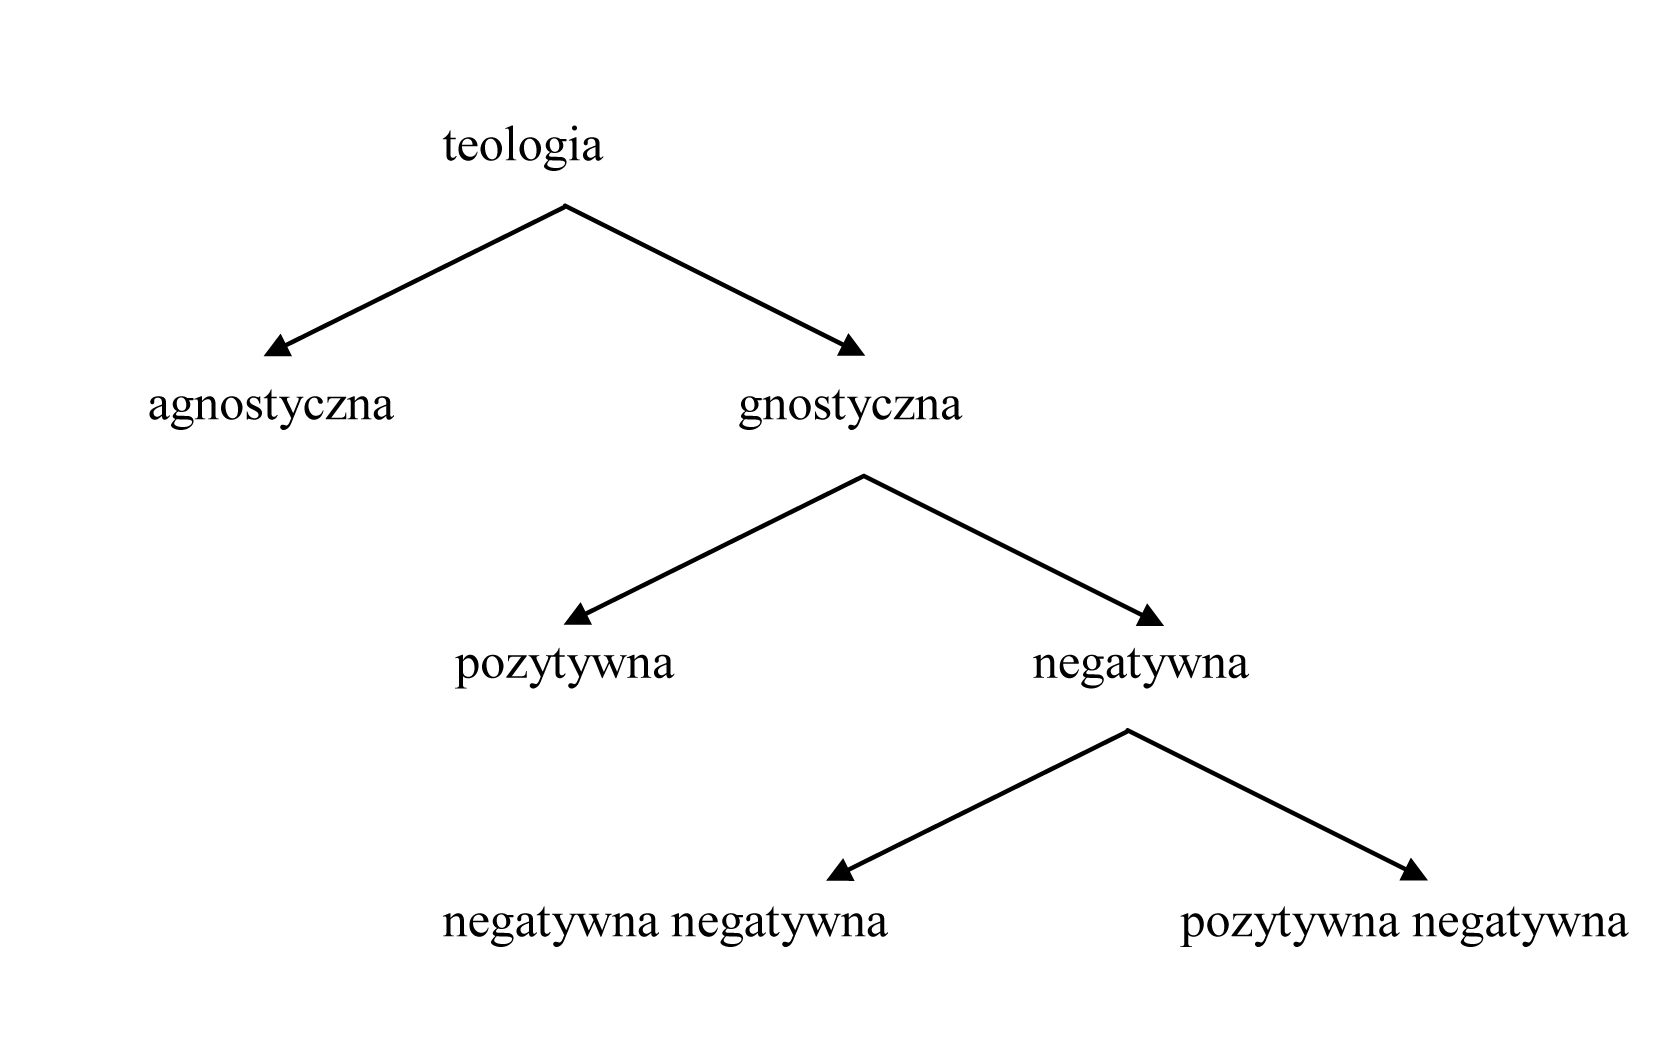
\includegraphics[width=1\linewidth]{typologia.jpg}
%\caption{Proponowana przez Rojka
%typologia interpretacji teologii apofatycznej.}
%}
%\end{figure}

%\begin{figure}[H]
%\begin{center}
% \begin{tikzpicture}[node distance=1cm]
%
%    \node (1) {teologia};
%    \node (21) [below=of 1, xshift=-2.5cm] {agnostyczna};
%    \node (22) [below=of 1, xshift=2.5cm] {gnostyczna};
%    \node (31b) [below=of 22, xshift=-2.5cm] {pozytywna};
%    \node (32b) [below=of 22, xshift=2.5cm] {negatywna};
%    \node (41) [below=of 32b, xshift=-2.5cm] {negatywna negatywna};
%    \node (42) [below=of 32b, xshift=2.5cm] {pozytywna negatywna};
%
%    \path[-] (1) edge (21);
%    \path[-] (1) edge (22);
%    \path[-] (22) edge (31b);
%    \path[-] (22) edge (32b);
%    \path[-] (32b) edge (41);
%    \path[-] (32b) edge (42);
%
%\end{tikzpicture}
%
%\caption[Typologia teologii apofatycznej według Rojka]{Proponowana przez Rojka
%typologia interpretacji teologii apofatycznej.}\label{roj-typ-rys}
%\end{center}
%\end{figure}

%Problemem, któremu Rojek poświęca nieco uwagi, lecz mimo wszystko
%postanawia go nie rozstrzygać, jest problem własności pozytywnych. Jest
%to problem poważny, ponieważ w świetle przedstawionej powyżej typologii
%różnica między teologią pozytywną i negatywną polega na orzekaniu o
%najwyższej istocie pozytywnych własności lub ich negacji. Jak
%zdefiniować zbiór takich własności? Rojek wymienia kryterium
%syntaktyczne, które miałoby polegać na ,,obecności negacji w
%predykacie''\footnote{Tamże, s. 221. }. Nie do końca wiadomo, jak
%rozumieć takie kryterium. Przypuszczam, że formalnie można zapisać tę
%propozycję w logice predykatów II-rzędu w następujący sposób:
%
%\begin{equation}
%    P(Q) {=}_{df} \forall x \neg \exists N (Q(x) \equiv \neg N(x)),
%\end{equation}
%gdzie $P(Q)$ oznacza ,,własność $Q$ jest pozytywna''. Jednakże Rojek
%natychmiast dodaje, że kryterium syntaktyczne nie może być uważane za
%wystarczające. Powołuje się tu na klasyczny przykład predykatu ,,jest
%ślepy'' -- nie zawiera on negacji, lecz odnosi się do braku i z tego
%powodu wydaje się być pozytywny. Trafniejszym argumentem wydaje się być
%powołanie na św. Tomasza, wedle którego własności tradycyjnie
%przypisywane bytowi absolutnemu, takie jak prostota, doskonałość czy
%jedność, są w istocie własnościami negatywnymi\footnote{św. Tomasz z
%Akwinu Teologiczna: I, 3, Summa contra Gentiles 11. }.
%
%Problem własności pozytywnych Rojek pozostawia nierozwiązany tłumacząc,
%że skupia się na formie teologii negatywnej, nie na jej treści. Dodaje
%jednak, że istnieje jeszcze jeden bardzo szczególny sposób ich
%rozumienia. Można je traktować, jako najwyższy sposób istnienia danej
%własności, czyli tzw. perfekcje. Najczęściej mówi się o takich
%perfekcjach, jak wszechwiedza -- najwyższy sposób wiedzy, czy też
%wszechmoc -- najwyższy stopień mocy. Są one istotnym elementem w
%ontologicznych dowodach istnienia Boga, które w historii były
%proponowane m.in. przez św. Anzelma, Kartezjusza, Leibniza, Gödla i
%Perzanowskiego. W tych argumentach Boga można uznać za podmiot
%wszelkich własności pozytywnych rozumianych jako perfekcje:
%
%\begin{equation}
%    G(x) \equiv \forall Q (P(Q) \to Q(x)).
%\end{equation}
%
%
%Definicję tę Rojek zaczerpnął od Perzanowskiego\footnote{J.
%Perzanowski, Ontological Arguments II: Cartesian and Leibnizian, [w:]
%red. H. Burkhardt, B. Smith, Handbook of Metaphysics and Ontology, t.
%2, PhilosophiaVerlag, München 1991,ss.~625–633. } i stanowi ona
%wzór kolejnych definicji Boga w proponowanych przez niego następnie
%interpretacjach teologii negatywnej. Warto wiec poświęcić jej nieco
%uwagi. Po pierwsze, jest ona zapisana w rachunku predykatów drugiego
%rzędu, gdyż zawiera warunek, że własności przypisywane Bogu muszą być
%pozytywne. Po drugie, Bóg formalizowany jest jako predykat (,,$x$ jest
%Bogiem'', ,,$x$ jest bogopodobny''), nie jako stała logiczna\footnote{Por.
%choćby M. Durrant, The ,,Meaning of ‘God’-I, Royal Institute of
%Philosophy Supplement,vol. 31 (1992), ss. 71-84. }, lub deskrypcja
%określona, co proponował Bocheński\footnote{J.M. Bocheński, dz. cyt.,
%s. 381. }. Po trzecie, powyższa definicja powstała na użytek
%formalizacji dowodów ontologicznych, które należą raczej do jakiejś
%formy teologii pozytywnej. Zawarte w niej $P(Q)$ czytamy jako ,,$Q$ jest
%własnością pozytywną'' w pewnym szczególnym sensie opisanym powyżej -- ,,$Q$
%jest perfekcją''. Rojek nie sugeruje jednak, że w teologii apofatycznej
%Pseudo-Dionizego zaprzecza się jedynie tego typu własnościom
%pozytywnym. Przeciwnie, pisze wprost, że zakres negowanych własności
%jest szerszy\footnote{P. Rojek, dz. cyt., s. 222. }. Po raz
%kolejny jednak odżegnuje się od określenia, o jakie konkretnie
%własności chodzi. Jest to, moim zdaniem, jeden z najsłabszych punktów
%jego propozycji. Wrócę do tego ponownie w dyskusji.


\section{Agnostyczna teologia negatywna}\label{roj-agnostycna}

Strategią pierwszej przedstawianej przez Rojka\index[names]{Rojek, Paweł} apofatycznej teorii Boga
jest przyjęcie \eqref{rojek-T4} jako tezy podstawowej i odrzucenie lub
modyfikacja pozostałych tez, za cenę zachowania spójności.
Jak już ujawniliśmy, celem tego typu doktryny jest podkreślenie znaczenia
boskiej transcendencji -- teoria ta głosi, że Bóg jest zasadniczo niewyrażalny
i~niepojmowalny. Takie rozumienie teologii negatywnej jest popularne wśród wielu
komentatorów -- także tych, którzy rozważają logiczno-językową strukturę
tej teorii\footnote{Wśród nich Rojek\index[names]{Rojek, Paweł} wymienia Jerome'a Gellmana\index[names]{Gellman, Jerome I.}, Johna J.
Jonesa\index[names]{Jones, John J.} oraz Paula Rorema\index[names]{Rorem, Paul}. Zob., odpowiednio, rozdz. \ref{sil-gell} oraz \ref{sil-dionizy}.}.

%W rozważaniach Gellmana teologia negatywna jest teorią, w której
%jakikolwiek predykat P języka ,,skończonych bytów'' nie może być
%przedziwie orzekany o Bogu. Jej główną tezą jest, że Bóg nie należy do
%zakresu żadnego z predykatów naszego języka. Jeśli mówimy na przykład,
%że Bóg nie jest mądry, mamy na myśli raczej negacją
%\textit{wykluczającą}, niż negację \textit{wyboru}. Naszym zamiarem
%jest wyłącznie stwierdzenie, że to nieprawda, że predykat P przysługuje
%Bogu, niekoniecznie sugerując, że można o nim orzec dopełnienie tego
%predykatu, czyli nie-P\footnote{J.I. Gellman, The Meta-Philosophy of
%Religious Language. ,,No\^us'', nr 11 (1971), s. 158. }. Według
%Gellmana, zdanie ,,Bóg jest potężny'' teolog negatywny zrozumie jako
%negację dopełnienia predykatu ,,jest potężny''. W innym kontekście
%oznaczałoby to przypisanie obiektowi, o którym mowa, tej właśnie
%własności. Jednakże w przypadku Boga negowanie dopełnienia predykatu P
%nie oznacza przypisywania mu P. Mówiąc ogólnie, zdania języka
%religijnego negują dopełnienia wszystkich wymienianych przez nie
%własności Boga, który jest poza zakresem wszystkich naszych predykatów.
%One, z kolei -- będąc predykatami języka skończonych bytów -- z
%konieczności muszą oznaczać niedoskonałe własności\footnote{Zob.
%Tamże. }.
%
%Według Jonesa, teologia negatywna Pseudo-Dionizego Areopagity jest w
%dużej mierze teologią krytyczną. Polemizuje ona z błędnym sposobem
%mówienia o Bogu -- takim, który traktuje Go jak byty, czyli rzeczy lub
%pojęcia\footnote{J.J. Jones, dz. cyt., s. 357. }. Fakt, że Bóg
%przekracza wszelki byt, nadaje również strukturę językowi dyskursu
%teologicznego. Nie idzie tylko o to, że przypisywanie Bogu
%jakichkolwiek przymiotów przysługujących bytom jest z gruntu błędne.
%Zwykle, gdy mówimy o rzeczach, twierdzenia i przeczenia sprzeciwiają
%się sobie. W wykładni Dionizego nie dzieje się tak w przypadku Boga.
%Bóg nie jest jednym z bytów, zatem język służący do opisu bytów nie
%jest dla Niego właściwy. W wypracowanym przez niego języku teologicznym
%twierdzenia i zaprzeczenia należą do odmiennych grup, tworząc odmienne
%sposoby mówienia o Bogu. Ponieważ funkcjonują one w odmienny sposób,
%nie należy ich ze sobą mieszać. Te pierwsze przedstawiają Boga jako
%przyczynę wszystkiego, te drugie wyrażają jego transcendencję. Oba
%sposoby mówienia można stosować naraz zarówno do opisu Boga, jak i
%opisu przedmiotów, jednakże w ten sposób nie zdołamy wyrazić
%unikalności Boga -- tego, że jest czymś odrębnym od wszystkich
%bytów\footnote{Zob. Tamże, s. 360. }. Możemy tego dokonać
%wyłącznie przez negację, która według Jonesa jest kluczowym punktem
%myśli Dionizego. Istotnym jest, że Jones wyraźnie odróżnia negację od
%zaprzeczenia.
%
%
%\begin{quote}
%        W przeciwieństwie do zaprzeczenia, negacja odnosi się do (nie)możliwości
%poznania i powiedzenia czegokolwiek o Bogu. Jest to, jeśli można tak
%powiedzieć, reguła drugiego rzędu posługiwania się nazwami pierwszego
%rzędu.\footnote{Tamże, s. 381. Większą część tego cytatu podaję za
%Rojkiem, dz. cyt., s. 222. }
%\end{quote}






%Najbardziej agnostyczną interpretację dionizyjskiej teologii negatywnej
%zaproponował Paul Rorem. Podkreśla on podobieństwo teologii
%Pseudo-Dionizego z późną filozofią neoplatońską. W obu tych doktrynach
%byty uporządkowane są względem pewnej hierarchii i w celu dotarcia do
%bytu absolutnego należy ,,wspiąć się'' po tej ,,drabinie'' bytów. By
%spotkać Boga należy wpierw zanegować nasze wrażenia i wyobrażenia i
%przekroczyć je, by dojść do ich pojęciowych znaczeń. Następnie
%zanegowane zostać powinny także owe znaczenia oraz wszelkie inne
%pojęcia umysłu, ponieważ przekroczenie naszej wiedzy prowadzi do
%niepoznawalnego, do cichego zjednoczenia z Bogiem. Innymi słowy, Rorem
%zwraca uwagę, że u Areopagity drogą do Boga jest zaprzeczenie
%wszystkich bytów. Dionizy jednak wielokrotnie stwierdza, że Bóg jest
%także ponad wszelkim zaprzeczeniem. Ostatecznie więc, należy zanegować
%także wszelkie negacje, nie pozostawając już żadnym pojęciem
%Boga\footnote{Por. P. Rorem, Pseudo-Dionysius. A Commentary on the
%Texts and an Introduction to Their Influence, Oxford University Press,
%Oxford -- New York 1993, ss. 210-211. }. Jak zauważa Rorem, Dionizy
%,,zaprzecza i wykracza poza wszystkie nasze pojęcia lub «pojęciowe»
%atrybuty Boga i kończy na odrzuceniu wszelkiego mówienia i myślenia,
%nawet negatywnego''\footnote{Tenże, przypis do Pseudo-Dionizy
%Areopagita, The Complete Work, tłum. C. Luibheid,. Paulist Press, New
%York 1987, s. 99. Cytuję za P. Rojek, dz. cyt. }.





Wynikiem agnostycznej
interpretacji teologii negatywnej nie jest zatem twierdzenie, że Bóg posiada
własności negatywne. Stosunek Boga do własności -- czy to pozytywnych, czy negatywnych -- jest tu irrelewantny lub raczej niemożliwy do określenia. Główną tezą tej doktryny jest właśnie twierdzenie, że Bóg jest niewyrażalny i~niepoznawalny. 
Zgodnie ze wskazaną w~ten sposób dwuznacznością tezy \eqref{rojek-T4},
Rojek\index[names]{Rojek, Paweł} wyróżnia dwie wersje tej teorii. Wedle pierwszej z nich, Bóg jest
niewyrażalny, nie sposób go wysłowić.
%Konsekwentnym rozwinięciem tej
%teorii jest stwierdzenie, że dyskurs religijny jest pozbawiony
%jakiegokolwiek znaczenia.
Wedle drugiej wersji, Bóg jest
niepoznawalny, nie można posiąść o nim wiedzy.
%I choć dyskurs religijny
%posiada w tej teorii jakieś znaczenie, może on opisać wyłącznie to,
%czego o Bogu nie wiemy. Rojek omawia obie wersje tej interpretacji.
A zatem poruszamy się tutaj na gruncie dobrze nam znanej teologii milczenia, choć po raz pierwszy wyraźnie zaznaczony zostaje
wątek związany z niepoznawalnością Boga. Jak przekonuję w kolejnej części pracy\footnote{Zob. rozdz. \ref{scep}.}, teorię Niepoznawalnego należy
uważać za odrębną interpretacje teologii negatywnej. Umieszczenie tego fragmentu analiz Rojka\index[names]{Rojek, Paweł} w niniejszym rozdziale posiada jednak dodatkowe motywacje.
Po pierwsze, model tej teorii jest dla Rojka\index[names]{Rojek, Paweł} inspiracją w~budowaniu logicznej ramy dla jego własnej interpretacji -- pozytywnej teologii negatywnej. Bez przedstawienia sposobu, w~jaki Rojek\index[names]{Rojek, Paweł} dochodzi do logicznej rekonstrukcji teorii Niepoznawalnego, sprawozdanie z jego oryginalnego modelu straciłoby na jasności.
Po drugie, w~apofatycznej doktrynie Pseudo-Dionizego Areopagity\index[names]{Pseudo-Dionizy Areopagita}, która jest źródłem tez \eqref{rojek-T1}-\eqref{rojek-T4}, będących podstawą wszystkich rozważanych w niniejszym rozdziale teorii Boga, różnica między jego niewysławialnością a niepoznawalnością nie jest wyraźnie zarysowana.
Po trzecie, dosyć nietypowa syntaktyka zaproponowana przez Rojka\index[names]{Rojek, Paweł} do formalizacji teorii Niepoznawalnego nie posiada jednoznacznie epistemicznej natury, a~jej filozoficzne motywacje i~charakterystyka zdradzają symptomy świadczące, że w~tym przypadku wciąż pozostajemy na gruncie teologii milczenia.
W~końcu, do tego samego wniosku prowadzą nas Rojka\index[names]{Rojek, Paweł} komentarze do modelu teorii Niepoznawalnego, według których niepoznawalność Boga polega na niemożliwości \textit{twierdzenia}, że posiada on pozytywne własności.




\subsubsection{Teoria Niewysławialnego}\label{rojek-bochenski}

Teorię Niewysławialnego Rojek\index[names]{Rojek, Paweł} charakteryzuje zgodnie z duchem prezentowanej w~niniejszej części pracy teologii milczenia. Poprawnie identyfikuje jej paradoksalny charakter mający swe źródła w~samozwrotności.
Do jej rekonstrukcji adaptuje metajęzykowe ujęcie zaczerpnięte od Bocheńskiego\index[names]{Bocheński, Józef Maria}. Z~tego względu podstawową dla tej interpretacji teologii negatywnej tezę \eqref{rojek-T4} oddaje za Bocheńskim\index[names]{Bocheński, Józef Maria} jako
\begin{flalign*}
&G(x) \equiv \forall \mathcal{L}\ N_w(x,\mathcal{L}).&\tag{MNT''}\label{rojek-MNTbis}
\end{flalign*}

Rojek\index[names]{Rojek, Paweł} wydaje się być usatysfakcjonowany ustaleniami Bocheńskiego\index[names]{Bocheński, Józef Maria} i przekonany, że ujęcie teologii milczenia w postaci \ref{rojek-MNTbis} ratuje tę teorię przed sprzecznościami\footnote{Jak pokazałem w poprzednim rozdziale (rozdz. \ref{sil-boch-dyskusja}), można mieć co do tego wątpliwości.}.
Powyższą formułę wraz dodatkowymi uwagami głoszącymi, że mamy tu do czynienia z~wypowiedzią metajęzykową, nazywa ,,modelem'' teorii Niewysławialnego. Przyjmuje też w pełni Bocheńskiego\index[names]{Bocheński, Józef Maria} argumenty przeciwko teorii Niewysławialnego -- fakt, że nie możemy przypisać Bogu żadnej własności przedmiotowo-językowej sprawia, że teoria ta jest niezgodna z faktycznym dyskursem religijnym i religijną \textit{praxis}, a~więc dyskwalifikuje ją jako poprawną teorię Boga. Ze względu na jej uwikłanie w~swoje ,,zewnętrzne'' paradoksy należy ją odrzucić.



%Podobnie argumentuje John Hick, który uważa, że nie ma sensu
%
%
%\begin{quote}
%mówić o X, że żadne nasze pojęcie się do niego nie stosuje. Jest bowiem
%w oczywisty sposób niemożliwe odnosić się do czegoś, co nie posiada
%nawet własności 'bycia możliwym przedmiotem
%odniesienia.\footnote{J. Hick, An Interpretation of Religion. Human
%Responses to the Transcendent, Yale University Press, New Haven –
%Londyn 1989, s. 239. Cytuję za P. Sikora, Logos Niepojęty, Wydawnictwo
%Universitas, Kraków 2010, s. 118. }
%\end{quote}
%
%
%Dodaje on także, że określenie
%
%\begin{quote}
%,,taki, że nasze pojęcia się do niego nie stosują'' nie może,
%jeśli chcemy uniknąć paradoksu, odnosić się do własności, którą
%opisuje.\footnote{Tamże. }
%\end{quote}
%
%Przeciwko takiemu przedstawianiu teorii Niewysławialnego występuje Józef
%Maria Bocheński. Twierdzi on, że da się ją uratować od sprzeczności,
%lecz nawet mimo tego, nie odpowiada ona potrzebom dyskursu
%religijnego\footnote{Zob. J.M. Bocheński, dz. cyt., ss. 353-356.
%}. Bocheński uważa, że jeśli przestrzega się pewnych obowiązujących w
%logice konwencji, zarzut sprzeczności stawiany teorii Niewysławialnego
%przestanie obowiązywać. Należałoby wpierw dowieść, że danym układzie
%odniesienia teoria ta prowadzi do sprzeczności, tymczasem nikt takiego
%dowodu nie przedstawił. Według Bocheńskiego sytuacja przedstawia się
%zupełnie przeciwnie -- nietrudno wykazać, że teoria Niewysławialnego
%jest spójna. Poniżej przedstawię jego argumentację.
%
%Załóżmy, że dwuargumentowy predykat  $Nw(x,l)$ oznacza ,,$x$ jest
%niewyrażalne w języku $l$''.
%
%Zapiszmy teraz formułę zawierającą ten predykat
%
%\begin{equation}
%    \exists x \exists l Nw(x, l)
%\end{equation}
%
%
%Wydaje się, że nie tylko można ją wypowiedzieć nie popadając w
%sprzeczność, lecz także jest ona prawdziwa, nietrudno znaleźć taki
%obiekt $x$ i taki język $l$, które spełniałyby zapisany wyżej warunek.
%(Bocheński podaje przykład krowy i języka szachów: nie da się opisać
%krowy w języku szachów).
%
%Możemy powyższy przykład uogólnić i sformułować metajęzykową definicję
%Boga o następującej postaci:
%
%\begin{equation}\tag{G2}
%    G(x) \equiv \forall l Nw(x, l)\footnote{Definicję podaję za
%Rojkiem, różni się ona od zapisu Bocheńskiego tym, że u tego ostatniego
%,,Bóg'' zapisany został jako stała logiczna: $\forall l Nw(a, l)$.}
%\end{equation}
%
%
%
%Na pierwszy rzut oka, wydaje się, ze ta formuła jest bardziej
%problematyczna -- twierdzenie, że $x$ jest niewysłowione w żadnym języku
%zdaje się prowadzić do sprzeczności. Można jednak uniknąć tego
%problemu, stosując zwykłe konwencje wykorzystywane do pozbywania się
%antynomii semantycznych. Należy założyć, że żadne zdanie traktujące o
%pewnej klasie języków, nie jest formułowane w żadnym z tych języków.
%Aby było pozbawione sprzeczności musi zostać sformułowane w innym
%języku, czyli odpowiednim metajęzyku. Możemy więc założyć, że klasa
%języków wspominana w (G2) jest klasą języków przedmiotowych. W takim
%wypadku (G2) jest zdaniem metajęzyka pierwszego stopnia. Po takim
%zabiegu, sformułowana definicja jest znacząca i pozbawiona
%sprzeczności. Nie ma bowiem niespójności w twierdzeniu, że coś nie daje
%się wysłowić w jakimś języku, lub nawet w klasie języków, o ile
%twierdzenie to jest w języku nienależącym do tej klasy. Według
%Bocheńskiego, przy takim założeniu, standardowym z punktu widzenia
%logiki ogólnej, teoria Niewysławialnego pozostaje znacząca i spójna a
%zarzut sprzeczności zostaje oddalony.
%
%Bocheński odrzuca jednak teorię Niewysławialnego z co najmniej dwóch
%powodów. Po pierwsze, na mocy (G2) nie można przypisać Bogu
%jakiekolwiek własności językowo przedmiotowej. Jedyną własnością, jaką
%możemy mu przypisać, jest metajęzykowa własność bycia niewysłowionym w
%żadnym z języków przedmiotowych. W takim wypadku wierny, nie mógłby
%akceptować żadnego zdania dyskursu religijnego, które przypisałoby Bogu
%jakąkolwiek własność-przedmiotowo-językową. Wydaje się to niespójne z
%faktycznym dyskursem religijnym. Po drugie, niemożliwe byłoby oddawanie
%czci obiektowi, o którym wiemy tylko i wyłącznie, że nie można o nim
%nic powiedzieć. Jeśli wierny miałby czcić obiekt pozbawiony własności
%przedmiotowo-językowych, równie dobrze tym obiektem mógłby nie być Bóg
%a szatan\footnote{Por. J.M. Bocheński, dz. cyt., ss. 354-356. }.

%Rojek dodaje do tego podobny argument, jednakże umieszczony w kontekście
%teologii negatywnej. Mianowicie, jeśli teoria Niewysławialnego ma być
%właściwą interpretacją teologii negatywnej, można poddać w wątpliwość
%zasadność jednoczesnego utrzymywania tez \eqref{rojek-T1}-\eqref{rojek-T3}. Jeśli Bóg jest
%niewyrażalny, cały język religijny jest pozbawiony znaczenia, nie
%możemy więc ani sensownie potwierdzić, ani zaprzeczyć żadnym z Jego
%własności. Dla Rojka jest to wskazówka, by \eqref{rojek-T4} nie interpretować
%semantycznie, lecz epistemologicznie lub nawet
%ontologicznie\footnote{Zob. P. Rojek, dz. cyt., s. 223.}. W ten sposób przechodzi od
%teorii Niewysławialnego do agnostycznej teorii Niepoznawalnego.

Rojek\index[names]{Rojek, Paweł} dodaje do tego argument sformułowany w kontekście
swoich analiz. Mianowicie, jeśli teoria Niewysławialnego ma być
właściwą interpretacją teologii negatywnej, należy podać w wątpliwość
zasadność utrzymywania tez \eqref{rojek-T1}-\eqref{rojek-T3}. Jeśli Bóg jest
niewyrażalny, cały język religijny jest pozbawiony znaczenia, nie
możemy więc ani sensownie potwierdzić, ani zaprzeczyć żadnym z jego
własności. Krótko mówiąc, teoria Niewysławialnego zdaje się nie dawać żadnych szans na
akceptację którejkolwiek z wyabstrahowanych tez teologii apofatycznej poza \eqref{rojek-T4}.
Dla Rojka\index[names]{Rojek, Paweł} jest to wskazówka, by nie interpretować tej tezy
semantycznie, lecz epistemologicznie lub nawet
ontologicznie\footnote{Zob. P. Rojek, \textit{Logika teologii negatywnej}, dz. cyt., s. 223.}. W ten sposób przechodzi od
teorii Niewysławialnego do agnostycznej teorii Niepoznawalnego.


\subsubsection{Agnostyczna teoria Niepoznawalnego}

Według Rojka\index[names]{Rojek, Paweł} teoria Niepoznawalnego jest lepszym modelem teologii apofatycznej,
ponieważ nie tylko przyjmuje \eqref{rojek-T4} za twierdzenie podstawowe, lecz także
umożliwia pewną interpretację tez \eqref{rojek-T2} oraz \eqref{rojek-T3}. By to pokazać,
wprowadza pojęcie nieokreśloności oraz definiuje nowe, odmienne od
klasycznego pojęcie negacji. W tym celu wykorzystuje on logiczną teorię
nieokreśloności, którą na potrzeby modelowania (w~filozofii) nauki rozwinął
rosyjski logik Aleksander Zinowjew\index[names]{Zinowjew, Aleksander}\index[names]{Zinowjew, Aleksander}\footnote{A.A. Zinov'ev, \textit{Foundations
of the Logical Theory...}, dz. cyt. Zob. także tenże,
\textit{Logika nauki}, dz. cyt. }.

Filozoficzną motywacją logiki Zinowjewa\index[names]{Zinowjew, Aleksander} są  pewne ,,nieklasyczne'' przypadki
spotykane w teoriach i wynikach naukowych oraz ich interpretacjach, w których zniesione zostaje
prawo wyłączonego środka. Takie przypadki polegają na dopuszczeniu
możliwości istnienia obiektów, co do których nie da się ustalić, czy
posiadają one jakąś własność $Q$, czy też posiadają własność
$\neg Q$. Można do nich zaliczyć na przykład rozważaną
w~mechanice kwantowej cząstkę elementarną, której parametry -- zgodnie z
zasadą nieoznaczoności~-- nie mogą zostać ustalone\footnote{Interesujące może okazać się zbadanie związków pewnych rozwiązań wypracowanych w~ramach
teologii negatywnej
oraz filozofii mechaniki kwantowej.
Tym, którzy podają w wątpliwość teoretyczną wartość teologii negatywnej,
istnienie innych obszarów, w których możliwości ludzkiego języka i pojęć zdają się być niewystarczające, może dostarczyć argumentu
na rzecz wiarygodności tej doktryny jako teologicznej teorii tego, nie niewysławialne i niepojmowalne.
},
twierdzenie, które
na gruncie danego rachunku logicznego nie może zostać ani dowiedzione,
ani obalone, albo po prostu obiekt zmieniający się w~czasie. Na
potrzeby takich przypadków Zinowjew\index[names]{Zinowjew, Aleksander} nad logiką klasyczną wprowadza nowy funktor nieokreśloności i
oznacza go symbolem $?$\footnote{Dla utrzymania spójności zapisu, formuły teorii
nieokreśloności Zinowjewa\index[names]{Zinowjew, Aleksander} przedstawiam w~nieco zmodyfikowanej notacji zaproponowanej przez
Rojka\index[names]{Rojek, Paweł}.}. Niech zapis $?Q(x)$ oznacza ,,nie można
ustalić, czy $x$ ma $Q$, czy $x$ ma nie-$Q(x)$'', co można czytać także jako ,,$x$ ma w sposób
nieokreślony $Q$''. W~teorii Niepoznawalnego Bóg uznawany jest za
obiekt, którego nie da się poznać. Rojek\index[names]{Rojek, Paweł} proponuje, by za pomocą powyższego funktora nieokreśloności z logiki Zinowjewa\index[names]{Zinowjew, Aleksander}
podać nową definicję Boga jako obiektu, który wszystkie pozytywne
własności posiada w~sposób nieokreślony.
\begin{flalign*}
&G(x) \equiv \forall Q (P(Q) \to ?Q(x)).&\tag{ZNT}\label{rojek-ZNT}
\end{flalign*}
%\begin{equation}\tag{G3}
%   G(x) \equiv \forall Q (P(Q) \to ?Q(x)).
%\end{equation}

%
%
%Formule tej należy poświęcić nieco uwagi. Po pierwsze, w odróżnieniu od
%\ref{sil-boch-MNT} powyższa definicja nie jest wyrażona w metajęzyku, lecz w języku
%przedmiotowym. Po drugie, co istotniejsze, by uniknąć kłopotów z
%formalizowaniem Boga przy użyciu predykatu $G(x)$, należy ją ograniczyć.
%Do tej definicji trzeba dołożyć dodatkowe założenie, o postaci:
%
%\begin{equation}
%    \neg P(G)
%\end{equation}
%
%
%Innymi słowy, należy założyć, że predykat ,,jest Bogiem'' (lub ,,jest
%bogopodobny'') nie należy do zbioru predykatów pozytywnych. W
%przedziwnym bowiem razie, wpadlibyśmy w błędne koło i o niczym nie
%można byłoby określić, że jest Bogiem.

Jak twierdzi Rojek\index[names]{Rojek, Paweł}, wykorzystując ten formalizm do modelowania teorii
Niepoznawalnego, można -- w pewnym szczególnym sensie -- zaprzeczyć, że
Bóg posiada wszystkie własności pozytywne.
%Oczywiście, nie idzie tutaj
%o stwierdzenie, że o Bogu można na orzec jakiekolwiek
%$\neg Q$, przy założeniu, że $Q$ jest własnością pozytywną.
%Taki przypadek jest niezgodny zasadą \ref{rojek-ZNT}.
Idzie o to, że po
wprowadzeniu funktora nieokreśloności $?$, zdanie
,,nieprawda, że $x$ jest
$Q$''\footnote{Rojek mówi o wyrażeniu ,,$x$ jest nie-$Q$'', moim zdaniem
błędnie. W ogóle w przedstawieniu teorii Niepoznawalnego w szacie logiki nieokreśloności Zinowjewa\index[names]{Zinowjew, Aleksander} odnaleźć można dużo niezgrabności. Por. P.~Rojek, \textit{Logika teologii negatywnej}, dz. cyt., s.~223. Kładę to jednak na karb nietypowej notacji stosowanej przez radzieckiego logika, którą Rojek\index[names]{Rojek, Paweł} próbuje przeredagować według bardziej współczesnych standardów.} staje się dwuznaczne. Może ono przyjąć jedno
z dwóch znaczeń: albo ,,$x$ jest nie-$Q$'', albo ,,nie można stwierdzić, czy $x$~jest~$Q$''. W nomenklaturze Rojka\index[names]{Rojek, Paweł}, w pierwszym przypadku w~zdaniu pojawia
się negacja w~znaczeniu \textit{de dicto}, o~drugim znaczeniu natomiast
można mówić, że zawiera ono negację \textit{de re}. Nieco inne
nazewnictwo wprowadził Zinowjew\index[names]{Zinowjew, Aleksander}, który pierwszy rodzaj negacji nazwał
negacją zewnętrzną -- odnosi się ona bowiem do całego negowanego w~ten
sposób zdania, drugą negację nazwał
negacją wewnętrzną -- dotyczy ona bowiem wyłącznie predykatu\footnote{Konkretnie: operatora predykatywności.
Notacja zaproponowana przez Rojka\index[names]{Rojek, Paweł} pozbawiona jest już symbolu takiego operatora.}.

Przyjmijmy teraz dwa różne symbole, w celu odróżnienia odmiennych pojęć
negacji. Niech $\neg$ oznacza negację zewnętrzną,
natomiast symbol $\sim$ negację wewnętrzną. Przy
takiej notacji, formułę ${\sim}Q(x)$ czytamy jako ,,$x$ jest
nie-$Q$'', lub  inaczej: ,,$x$ ma własność nie-$Q$''\footnote{U Rojka\index[names]{Rojek, Paweł}: ,,$x$ ma
własność $\neg Q$''. }, natomiast formuła
$\neg Q(x)$\footnote{Rojek używa tych symboli na odwrót, to jest $\neg$ stosuje na oznaczenie negacji
wewnętrznej, a~$\sim$~używa do oddania negacji zewnętrznej. Dodatkowo formułę negowaną za pomocą
funktora negacji zewnętrznej opatruje w dodatkowe nawiasy po to, by
podkreślić odmienny, ,,zewnętrzny'' charakter tego rodzaju negacji.
Uznaję ten zabieg za redundantny i niekonieczny. Notacja Rojka\index[names]{Rojek, Paweł} jest odmienna od
stosowanej oryginalnie przez Zinowjewa\index[names]{Zinowjew, Aleksander}.} oznacza ,,nieprawda, że $x$~jest $Q$'', lub ,,nie twierdzi się, że
$x$~ma własność $Q$''. Poniższe aksjomaty definiują relacje, jakie zachodzą
pomiędzy funktorem nieokreśloności a funktorami negacji wewnętrznej i~zewnętrznej\footnote{Aksjomaty podaję za Rojkiem\index[names]{Rojek, Paweł}, bez żadnej kwantyfikacji i konsekwentnie trzymam się tej konwencji.}:
\begin{flalign*}
&\neg Q(x) \equiv {\sim} Q(x)\ \lor\ ?Q(x),&\tag{Z\textsubscript{1}}\label{rojek-zin1}\\
&\neg {\sim} Q(x) \equiv Q(x)\ \lor\ ?Q(x),&\tag{Z\textsubscript{2}}\label{rojek-zin2}\\
&\neg ?Q(x) \equiv Q(x)\ \lor\ {\sim} Q(x)  .&\tag{Z\textsubscript{3}}\label{rojek-zin3}
\end{flalign*}
%\begin{equation}\tag{Z1}
%\neg  Q(x) \equiv ?Q(x) \lor {\sim} Q(x),
%\end{equation}
%\begin{equation}\tag{Z2}
%\neg {\sim} Q(x) \equiv Q(x)\ \lor\ ?Q(x),
%\end{equation}
%\begin{equation}\tag{Z3}
%\sim ?Q(x) \equiv Q(x) \lor {\sim} Q(x).
%\end{equation}
Z \eqref{rojek-zin3} oraz prawa De Morgana\index[names]{De Morgan, Augustus} bezpośrednio wynika:
\begin{flalign}
& ?Q(x)\ \equiv\ \neg  Q(x)\ \land\ \neg {\sim} Q(x). &\label{rojek-zin4}
\end{flalign}
%\begin{equation}
%   \vdash \quad ?Q(x)\ \equiv\ \neg  Q(x)\ \land\ \neg {\sim} Q(x).
%\end{equation}
 



Gdybyśmy chcieli dokonać kolapsu z powrotem do logiki klasycznej,
musielibyśmy założyć, że (dla każdego $x$, dla dowolnego $Q$) zachodzi $\neg ? Q(x)$. Prawdziwe jest bowiem twierdzenie

\begin{flalign}
&  \neg ?Q(x)\ \to \big({\sim} Q(x) \equiv \neg Q(x)\big).&
\end{flalign}
Przy założeniu, że nie istnieją przypadki nieokreśloności, negacje \textit{de re} i \textit{de
dicto} stają się tożsame.
Jednakże, jeśli
chcemy opisać wspomniane wyżej przypadki nieklasyczne, w~których
posiadanie lub nieposiadanie danej własności przez jakiś obiekt
nie może zostać określone, musimy zgodzić się na obecność dwóch
różnych, nierównoważnych pojęć negacji w systemie. Z tego powodu
poniższa formuła nie jest wyprowadzalna w ramach prezentowanego tu systemu:
\begin{flalign}
& \nvdash  \neg  Q(x) \to  {\sim} Q(x). &
\end{flalign}
%
%\begin{equation}
%    \nvdash \quad \neg  Q(x) \to  {\sim} Q(x).
%\end{equation}
Dzieje się tak, ponieważ $\neg Q(x)$ pociąga za sobą ${\sim} Q(x)$ lub
$?Q(x)$. Analogicznie, w~prezentowanym tu rachunku nie zachodzi
następująca wersja prawa podwójnej negacji
\begin{flalign}
& \nvdash   \neg  {\sim} Q(x) \to  Q(x), &
\end{flalign}
%
%
%\begin{equation}
%   \nvdash   \neg  ({\sim} Q(\textit{x})) \to  Q(\textit{x}),
%\end{equation}
ponieważ $\neg {\sim} Q(x)$ implikuje $Q(x)$ lub $?Q(x)$. Prawdziwe są
natomiast następujące formuły:
\begin{flalign}
&   {\sim} Q(x) \to  \neg  Q(x), &\\
&   Q(x) \to  \neg  {\sim} Q(x). &
\end{flalign}


%\begin{equation}
%    \vdash \quad {\sim} Q(x) \to  \neg  Q(x),
%\end{equation}
%\begin{equation}
%    \vdash \quad Q(x) \to  \neg  {\sim} Q(x).
%\end{equation}






Należy zauważyć, że dla negacji wewnętrznej nie można mówić
o ,,nieklasycznym'' prawie wyłączonego środka
\begin{flalign}
& \nvdash  Q(x) \lor {\sim} Q(x), &
\end{flalign}
%
%\begin{equation}
%     \nvdash \quad Q(x) \lor {\sim} Q(x),
%\end{equation}
ponieważ istnieje dodatkowa, trzecia możliwość -- $?Q(x)$. Do grona tez tego
rachunku należy zatem następująca formuła:
\begin{flalign}
&    Q(x) \lor  {\sim} Q(x)\ \lor\  ?Q(x). &
\end{flalign}
%\begin{equation}
%    \vdash \quad Q(x) \lor  {\sim} Q(x) \lor  ?Q(x)
%\end{equation}
Prawo wyłączonego środka obowiązuje natomiast dla negacji \textit{de
dicto}:
\begin{flalign}
&    Q(x) \lor  \neg  Q(x), &\\
&    {\sim} Q(x) \lor  \neg  {\sim} Q(x), &\\
&    ?Q(x) \lor  \neg  ?Q(x). &
\end{flalign}
%\begin{equation}
%    \vdash \quad Q(x) \lor  \neg  Q(x),
%\end{equation}
%\begin{equation}
%    \vdash \quad {\sim} Q(x) \lor  \neg  {\sim} Q(x),
%\end{equation}
%\begin{equation}
%\vdash \quad ?Q(x) \lor  \neg  ?Q(x).
%\end{equation}

Niewątpliwym wkładem Rojka\index[names]{Rojek, Paweł} jest spostrzeżenie, że rachunek Zinowjewa\index[names]{Zinowjew, Aleksander} stworzony pierwotnie na potrzeby
logicznej rekonstrukcji  pewnych teorii naukowych, w~ramach których naruszona zostaje reguła \textit{tertium non datur}, może okazać się przydatny także do modelowania
omawianej w tym paragrafie interpretacji teologii apofatycznej. Dzięki
 własnościom tego rachunku, można przedstawić w sposób niesprzeczny już trzy spośród
tez wypreparowanych z pism Pseudo-Dionizego Areopagity\index[names]{Pseudo-Dionizy Areopagita}. Rekonstrukcją
tezy \eqref{rojek-T4} w~obrębie tej interpretacji i w terminach rachunku Zinowjewa\index[names]{Zinowjew, Aleksander} jest definicja Boga podana przez \ref{rojek-ZNT}.
Z tejże formuły, na podstawie praw logiki Zinowjewa\index[names]{Zinowjew, Aleksander} nietrudno już wyprowadzić dwie kolejne tezy doktryny Dionizego\index[names]{Pseudo-Dionizy Areopagita}.

Negację, o której mowa
w \eqref{rojek-T2}, można traktować jako negację \textit{de dicto}, ponieważ
zgodnie z teorią Niepoznawalnego, nie możemy stwierdzić, czy
Bóg posiada jakieś własności\footnote{Ten fragment analiz Rojka\index[names]{Rojek, Paweł} jest trochę naciągany. Związane jest to z~narzuceniem specyficznej interpretacji na funktor ,,zwykłej'', zewnętrznej negacji \textit{de dicto} jako ,,nie można stwierdzić, że'', podczas gdy taka interpretacja prędzej przysługiwałaby funktorowi nieokreśloności. Jednakże biorę to rozumienie za dobrą monetę, a~słabe punkty analiz Rojka\index[names]{Rojek, Paweł} wskażę w innych miejscach.}. W takim podejściu, \eqref{rojek-T2} stwierdza, że o
Bogu można orzec zewnętrzne negacje wszystkich własności pozytywnych. A
zatem, w języku tego rachunku należałoby to zapisać w następujący sposób:
\begin{flalign}
&    G(x) \to  (\forall Q (P(Q) \to  \neg Q(x)). &\tag{T2'}\label{rojek-T2prim}
\end{flalign}
%
%
%\begin{equation}
%    G(x) \to  (\forall Q (P(Q) \to  \neg Q(x)).
%\end{equation}
%
%
%
Co więcej, powyższa formuła jest bezpośrednią konsekwencją definicji
\ref{rojek-ZNT} i (\ref{rojek-zin4}). Ponieważ negacja
\textit{de dicto} jest różna od negacji \textit{de re}, nie możemy
jednocześnie twierdzić, że Bóg posiada (wewnętrzną) negację wszystkich
pozytywnych własności, czyli że można o~nim orzekać każde nie-$Q$, o ile
$Q$ jest pozytywne. Z~obu tych formuł wynika
także
\begin{flalign}
&    G(x) \to  (\forall Q (P(Q) \to
\neg {\sim} Q(x)), &\tag{T3'}\label{rojek-T3prim}
\end{flalign}
%
%\begin{equation}
%    G(x) \to  (\forall Q (P(Q) \to
%\neg {\sim} Q(x)),
%\end{equation}
%
%
którą Rojek\index[names]{Rojek, Paweł} uważa  za zrekonstruowaną w ramach syntaksy Zinowjewa\index[names]{Zinowjew, Aleksander} tezę \eqref{rojek-T3}.
Formuła ta zawiera
podwójne przeczenie, jednakże pierwsza negacja ma charakter \textit{de
dicto}, natomiast druga jest negacją \textit{de re}. Brzmieniem tej
formuły jest ,,Nieprawda, że Bóg posiada wszystkie wewnętrzne negacje
pozytywnych własności''.

W takim wypadku, wszystkie stwierdzenia Dionizego\index[names]{Pseudo-Dionizy Areopagita} o tym, że Bóg nie jest
ani $Q$, ani nie-$Q$, na przykład że nie jest on ,,ani wielkością, ani
małością, ani równością, ani nierównością, ani podobieństwem, ani
niepodobieństwem'', ,,nie jest też niczym z niebytu ani czymś z
bytu''\footnote{Pseudo-Dionizy Areopagita, \textit{Teologia mistyczna}, dz.
cyt., rozdział V. } itp.,  można niesprzecznie interpretować w
ramach powyższej rekonstrukcji. Podobnie wypowiedzi Areopagity\index[names]{Pseudo-Dionizy Areopagita} o
tym, że Bóg jest ,,ponad wszelkim twierdzeniem i~ponad wszelkim
zaprzeczeniem''\footnote{Tamże.} można ująć w ramach
prezentowanego rachunku, jako koniunkcję warunków zawartych już
w~formułach \eqref{rojek-T2prim} i \eqref{rojek-T3prim}.
\begin{flalign}
&    G(x) \to  (\forall Q (P(Q) \to  \neg  Q(x) \land
\neg {\sim} Q(x)). &
\end{flalign}

%\begin{equation}
%    G(x) \to  (\forall Q (P(Q) \to  \neg  Q(x) \land
%\neg {\sim} Q(x)).
%\end{equation}



%Jak zauważa Rojek, istnieje wyjątek od konsekwentnego stosowania tej
%interpretacji. Nie można w ten sposób formalizować  twierdzeń, że Bóg
%nie jest ani poznawalny ani niepoznawalny, ani określony, ani
%nieokreślony. Taka treść predykatu $Q$ naraziłaby bowiem tę interpretację
%na sprzeczność. Jednakże wydaje się, że żadne z dzieł Dionizego nie
%zawiera podobnych sformułowań\footnote{Także Jones zauważa, że teza o
%niepoznawalności Boga ma wyjątkowy charakter w pismach Dionizego i
%nigdy nie występuje w podobnych parach. Zob. J.J. Jones, dz. cyt., s.
%358. }.


Rojek\index[names]{Rojek, Paweł} jest przekonany, że powyższe analizy chronią agnostyczną teologię negatywną przed
sprzecznościami, a~największą ich wadą jest to, że nie obejmują wszystkich tez wypreparowanych z pism Areopagity\index[names]{Pseudo-Dionizy Areopagita}.
Na tym gruncie teoria Niepoznawalnego wydaje się lepszą
interpretacją teologii negatywnej -- można w jej ramach
przyjąć aż trzy z apofatycznych tez. Teoria
Niewysławialnego ustępuje w tym zestawieniu  i obejmuje tylko jedną
tezę dionizyjskiej doktryny. Obie jednak zawodzą w interpretacji \eqref{rojek-T1}.
Teza ta nie znajduje swojego miejsca w agnostycznych 
interpretacjach, bowiem -- skoro Bóg jest niepoznawalny -- nie można o nim
nic sensownie stwierdzić.
Do tej uwagi Rojek\index[names]{Rojek, Paweł} dokłada argumenty Bocheńskiego przeciw teorii Niewysławialnego -- tym razem stosując je do obu interpretacji w ramach agnostycznej teologii negatywnej.
Są one zasadniczo niespójne z faktycznym dyskursem
i praktyką religijną. Zgodnie z ich duchem, wierny nie mógłby
akceptować żadnych zdań dyskursu religijnego, które przypisują Bogu
jakieś własności. Tymczasem każdy dyskurs religijny zawiera
przynajmniej kilka takich zdań. Poza tym, gdyby o Bogu nie można było
orzekać żadnych własności, nie mógłby on być przedmiotem wiary i~czci\footnote{
Zob. J.M. Bocheński, \textit{Logika religii}, dz. cyt., ss. 355-356, a~także rozdz. \ref{sil-boch-nonsens}.}.




\section{Negatywna teologia negatywna}

Wad tych pozbawiona jest druga interpretacja teologii negatywnej, którą
Rojek\index[names]{Rojek, Paweł} nazywa negatywną teologią negatywną. Jej punktem wyjścia jest
teza \eqref{rojek-T2}. Na gruncie tej interpretacji nie twierdzi się, że
dyskurs religijny pozbawiony jest znaczenia, ani że Bóg jest
niepoznawalny. Uważa się natomiast, że o przedmiocie religijnym można
orzekać wyłącznie negatywne własności. Nie jest więc tak, że nic nie
wiemy o Bogu -- wiemy, że nie posiada on pozytywnych własności.
%Należy
%przyznać, że jest to dość popularna interpretacja teologii
%apofatycznej. Na przykład, do właśnie w taki sposób rozumianej teologii
%negatywnej odnosił się Józef Maria Bocheński w dziele \textit{Logika
%religii}.

%W analizie Rojka, negację obecną w \eqref{rojek-T2}
%należy traktować w~zwykły, klasyczny sposób. Zatem \eqref{rojek-T1} oraz \eqref{rojek-T3} muszą zostać natychmiast odrzucone, jako niespójne z tezą przyjętą tu za podstawową.
Z drugiej strony, wedle tej wersji teologii negatywnej, wszystko, co możemy orzec o~Bogu,
posiada ściśle negatywny charakter. Na tym ma polegać boska transcendencja.
Choć taka teoria zatraca swój samozwrotny charakter (obecny w jakimś
stopniu w agnostycznej teologii negatywnej), w jej analizach nietrudno wskazać innego rodziaju sprzeczności. W~obrębie tej interpretacji Bóg
wciąż pozostaje w jakimś
sensie niepoznawalny -- jedyne, co o Nim wiemy to jaki nie jest. Można
więc pokusić się także na próbę uwzględnienia tezy \eqref{rojek-T4} w ramach modelu tej teorii.

Rojek\index[names]{Rojek, Paweł} twierdzi, że w tym modelu teologii negatywnej właściwą definicją
Boga jest formalizacja tezy \eqref{rojek-T2} w obrębie klasycznego rachunku
predykatów drugiego rzędu.
Skoro mamy do czynienia z~klasyczną negacją, \eqref{rojek-T1} oraz \eqref{rojek-T3} muszą zostać natychmiast odrzucone jako niespójne z tezą przyjętą tu za podstawową.
Bóg -- analogicznie do poprzednich definicji –
opisany jest jako obiekt, o którym można orzekać negacje wszystkich
pozytywnych własności:
\begin{flalign}
&    G(x) \equiv  \forall Q (P(Q) \to
\neg Q(x)). &\tag{NNT''}\label{rojek-NNTbis}
\end{flalign}

%\begin{equation}\label{G4}\tag{G4}
%    G(x) \equiv  \forall Q (P(Q) \to
%\neg Q(x)).
%\end{equation}


Powyższa definicja jest trawestacją zasady \ref{sil-boch-NNT} proponowanej przez Bocheńskiego\index[names]{Bocheński, Józef Maria}. Zatem wszystkie krytyczne uwagi formułowane w poprzednim rozdziale\footnote{Zob. rozdz. \ref{sil-boch-dyskusja}.} będą trafne także w przypadku omawianych tu rozważań Rojka\index[names]{Rojek, Paweł}. Zdaje się on być świadomy problemów nękających tę teorię Boga. Podaje zresztą zestaw ograniczeń, które należy do niej wprowadzić, by w proponowany model nie
wkradła się żadna sprzeczność. Najważniejsze ograniczenia dotyczą zbioru
pozytywnych własności. Jak wspominałem wcześniej, Rojek\index[names]{Rojek, Paweł} nie podaje
żadnej definicji, ani kryterium wyróżniania takich własności. Czyni jedynie na ten temat kilka uwag,
które w większym bądź mniejszym stopniu nawiązują do rozważań
Bocheńskiego\index[names]{Bocheński, Józef Maria}. Odniosę się jeszcze do tego w dyskusji.

Rojek\index[names]{Rojek, Paweł} zdaje się także nie dostrzegać, że jedna z implikacji składających się na \ref{rojek-NNTbis} jest identyczna z~\ref{rojek-T2prim}. Oczywiście, w logice Zinowjewa\index[names]{Zinowjew, Aleksander} wykorzystanej do formalizacji agnostycznej teologii negatywnej wyróżnialiśmy dwa pojęcia negacji. Negacja \textit{de re} zachowywała się odmiennie i~miała pewne nieklasyczne własności, ale to negacja \textit{de dicto} użyta w \ref{rojek-T2prim} była tą ,,zwykłą'', zachowującą się klasycznie negacją.

%Po pierwsze, według Rojka, zbiór pozytywnych własności nie może zawierać
%własności negatywnych. Szczerze powiedziawszy, nie jest do końca jasne
%także to, jak Rojek rozumie pojęcie własności negatywnej. W tym wypadku
%jednak mamy dość tradycyjną, syntaktyczną definicję tego pojęcia.
%Własność negatywna, zwana czasem także własnością dopełniającą, jest
%jedną z własności złożonych i stanowi po prostu negację własności. W
%języku naturalnym pojęcie negacji własności wrażamy prze użycie
%przedrostka \textit{nie}- (w języku łacińskim
%\textit{non}-)\footnote{Zob. J. Paśniczek, Predykacja, Copernicus
%Center Press, Kraków 2014. }. Wydaje się, że Rojek pojęcie
%własności negatywnej rozumie w podobny sposób, twierdzi bowiem, że nie
%stosując tego ograniczenia, doprowadzimy do orzekania o Bogu także
%własności pozytywnych (co z kolei sugeruje, że jest on także bliski
%stosowaniu syntaktycznej definicji własności pozytywnej -- jako
%niezawierającej spójnika negacji). Według Rojka, jeśli nie wprowadzimy
%tego ograniczenia, nasz model umożliwi pozytywne twierdzenia o Bogu,
%bowiem w przyjętej tu logice klasycznej $\neg \neg Q$
%implikuje $Q$. Ponadto uważa on, że dopuszczenie do
%zaprzeczania własności negatywnych wprowadzi do systemu sprzeczność,
%bowiem umożliwi orzekanie o Bogu zarówno $\neg Q$, jak i
%$\neg \neg Q$\footnote{Myślę, że
%konsekwencji tej można by uniknąć wprowadzając porządną definicję
%własności pozytywnych. Niestety, jak już zostało wspomniane, nie
%została ona podana. }. Jednakże dla Rojka syntaktyczne kryterium
%wyróżniania własności pozytywnych nie jest satysfakcjonujące.
%Alternatywą dla niego byłoby kryterium epistemologiczne, zaproponowane
%przez Bocheńskiego\footnote{J.M. Bocheński, dz. cyt., s. 416. }.
%Wedle tego kryterium własności pozytywne definiuje się indukcyjnie,
%jako własności postrzegane bezpośrednio lub zapisywane za pomocą
%formuł, zawierających wyłącznie symbole własności pozytywnych i terminy
%logiki pozytywnej. Rojek zgadza się z Bocheńskim, że także takie
%kryterium nie jest wystarczająco ścisłe. Nie zamierza jednak
%rozwiązywać tego problemu i podawać odpowiedniej definicji\footnote{
%Por. P. Rojek, dz. cyt., s. 226. }.
%
%Po drugie, po raz kolejny należy wykluczyć predykat ,,jest Bogiem'' ze
%zbioru predykatów oznaczających własności pozytywne. Uznanie własności
%bycia Bogiem za własność pozytywną doprowadziłoby do sprzeczności:
%
%\begin{equation}
%    G(x) \equiv \neg G(x).
%\end{equation}
%
%
%Wedle Rojka, twierdzenie ,,Bóg nie jest boski'' należy przeinterpretować w
%taki sposób, by w orzeczniku tego zdania nie znalazł się predykat $G(x)$,
%który użyty jest w (G4), lecz wiązka pozytywnych własności zwykle
%przypisywanych Bogu. W mojej opinii problem ten mógłby zostać
%rozwiązany poprzez formalizowanie Boga przy pomocy stałej logicznej,
%zamiast predykatu ,,$x$ jest Bogiem''.

Jeśli przymkniemy oko na wszystkie mankamenty podanej tu
definicji Boga, możemy doprowadzić ją do ciekawych filozoficznie
konsekwencji. Jak zauważa Rojek\index[names]{Rojek, Paweł}, zgodnie z omawianą wcześniej interpretacją Johna J.
Jonesa\index[names]{Jones, John J.}\footnote{Zob. rozdz. \ref{sil-dionizy}.}, głównym celem Dionizego\index[names]{Pseudo-Dionizy Areopagita} było wykazanie, że Bóg jest ponad
wszelkim bytem, w szczególności nie należy on do kategorii przedmiotów.
Według popularnego rozumienia przedmiotu, można traktować go jako
podmiot własności. Taką definicją posługiwał się na przykład Stanisław
Leśniewski\index[names]{Leśniewski, Stanisław}.

\begin{defin}[Przedmiot\footnote{,,Coś jest przedmiotem jeśli jest coś, czym to coś jest''. Rojek\index[names]{Rojek, Paweł} powołuje się tu na
dwa źródła: J.~Słupecki, \textit{Stanisław Leśniewski’s Calculus of Names},
,,Studia Logica'', nr 3 (1955), ss. 7-76 oraz J.~Perzanowski, \textit{The Way
of Truth}, [w:] \textit{Formal Ontology}, red. R. Poli, P. Simons, Kluwer
Academic Publishers, Dordrecht 1996, ss. 61-130.}]
Coś nazwiemy przedmiotem, o ile istnieje jakaś
własność, którą można o tym orzec:
\setlength{\abovedisplayskip}{0pt}
\begin{flalign*}
&     Ob(x) \equiv  \exists Q \ Q(x). &
\end{flalign*}
%\begin{equation}
%    Ob(x) \equiv  \exists Q  (Q(x)).
%\end{equation}
\end{defin}


Jeśli uzupełnimy tę definicję o warunek, że każdy przedmiot powinien
posiadać nie jakąkolwiek, ale pozytywną wartość, otrzymamy następującą
modyfikację\footnote{W świetle stawianych przez Rojka\index[names]{Rojek, Paweł} ograniczeń na definicję \ref{rojek-NNTbis}, 
konieczność wprowadzania w tę definicję dodatkowego zastrzeżenia wydaje
się wątpliwa.}:
\begin{defin}\label{rojek-object}
Coś nazwiemy przedmiotem, o ile istnieje jakaś pozytywna
własność, którą można o tym orzec:
\setlength{\abovedisplayskip}{0pt}
\begin{flalign*}
&     Ob(x) \equiv  \exists Q (P(Q) \land  Q(x)). &
\end{flalign*}
%\begin{equation}\label{D4}\tag{D4}
%    Ob(x) \equiv  \exists Q P(Q) \land  Q(x).
%\end{equation}
\end{defin}




Zgodnie z tak zmodyfikowaną definicją, Bóg nie należy do zbioru
przedmiotów, ponieważ nie może on posiadać żadnych pozytywnych
własności.
\begin{flalign}
&     \forall x (G(x) \to  \neg Ob(x))\footnote{U Rojka zmienna x nie jest związana
    żadnym kwantyfikatorem}. &
\end{flalign}
%\begin{equation}
%    \forall x (G(x) \to  \neg Ob(x))\footnote{U Rojka zmienna x nie jest związana
%    żadnym kwantyfikatorem}.
%\end{equation}
Rojek\index[names]{Rojek, Paweł} konkluduje, że gdy przyjmiemy powyższe rozważania za dobrą monetę,
Bóg istnieje w jakiś inny sposób, odmienny od tego, jak istnieją inne
byty.
%Według niego można tu mówić o istnieniu w sensie Quine’a (w
%przeciwieństwie do istnienia w sensie przedmiotów Leśniewskiego).
Konkluzja ta zdaje się być w zgodzie z  rozważaniami tych przedstawicieli
teologii negatywnej, którzy kładą akcent na transcendencję Boga -- to, że
przekracza on wszystkie byty. W~przedstawianym powyżej modelu nie można
go bowiem traktować jako przedmiot w sensie uchwyconym w definicji \ref{rojek-object}.

Czy Bóg zdefiniowany za pomocą \ref{rojek-NNTbis} jest poznawalny? W jakimś sensie
możemy wyrazić jego naturę -- możemy mówić, jaki nie jest. Z~drugiej strony,
uczciwie rzecz ujmując, na gruncie tego modelu  nie możemy posiąść
żadnej pozytywnej wiedzy o Bogu. Z~tego powodu w tej teorii znajdzie
się również miejsce na pewną interpretację tezy \eqref{rojek-T4}. Rojek\index[names]{Rojek, Paweł} ujmuje ją w
następujący sposób:



\begin{quote}
    W normalnym wypadku rozumiemy natury rzeczy przez porównanie ich z tym,
czym one nie są. Jak mawiał Spinoza\index[names]{Spinoza, Baruch}, ,,określenie jest negacją''. Bez
opozycji znaczeniowych i różnic nie moglibyśmy używać języka w sposób,
w jaki go faktycznie używamy. Bóg jako negacją wszelkich własności
znajduje się jednak poza całym systemem opozycji i różnic. Pełna
negacja prowadzi do całkowitego nieokreślenia\footnote{P. Rojek, \textit{Logika teologii negatywnej}, dz.
cyt., s. 226.}.
\end{quote}
A zatem w pewnym sensie także na gruncie tej teorii możemy mówić o
niepoznawalności czy nawet niewyrażalności Boga.

Powyższe rozważania, bez dodatkowych uściśleń (zwłaszcza adekwatnej definicji własności pozytywnych)
trudno określić mianem ,,modelu''. Tymczasem Rojek\index[names]{Rojek, Paweł} jest przekonany, że jest to model spójny, o ile tylko zgodzimy się na
wszystkie jego ograniczenia. Choć nie
uwzględnia on wszystkich tez wyabstrahowanych z dzieł Areopagity\index[names]{Pseudo-Dionizy Areopagita}, w
atrakcyjny sposób rozwija on tezę o wyłącznie negatywnym charakterze
wiedzy o Bogu. Ponadto, nie wymaga on stosowania wyrafinowanych
narzędzi formalnych, pozostając przy logice klasycznej. Jego dodatkowym
atutem jest pewna interesująca filozoficznie własność -- Bóg rozumiany
jest tu jako istotnie odmienny od całej dziedziny bytów rozumianych
jako przedmioty. Jednakże w takiej interpretacji nie ma miejsca na
rekonstrukcję tez \eqref{rojek-T1} oraz \eqref{rojek-T3}. Ponadto, jak Rojek\index[names]{Rojek, Paweł} podaje za Bocheńskim\index[names]{Bocheński, Józef Maria}, nie da się jej pogodzić z
dyskursem i praktyką religijną -- trudno jest bowiem oddawać cześć
czemuś, o czym wiemy tylko, czym nie jest\footnote{Jest to zarzut
stawiany przez Bocheńskiego\index[names]{Bocheński, Józef Maria}, \textit{Logika religii}, dz. cyt., s. 418.}.



\section{Pozytywna teologia negatywna}\label{roj-pozytywna}

Ostatnia interpretacja teologii negatywnej jest autorskim pomysłem
Rojka\index[names]{Rojek, Paweł}\footnote{Por. P. Rojek, \textit{Logika teologii negatywnej}, dz. cyt., ss. 227-230. }. Również na
jej gruncie, podstawową tezą teologii negatywnej jest \eqref{rojek-T2}. A zatem
o~Bogu można orzec wyłącznie własności negatywne. Ponieważ model
stosowany do formalizacji tej interpretacji używa pewnego
specyficznego, nieklasycznego pojęcia negacji (innego niż wprowadzona
we wcześniejszych paragrafach negacja \textit{de dicto}), może on
również zinterpretować w odpowiedni sposób także tezy \eqref{rojek-T1} oraz \eqref{rojek-T3}.
Model ten może również zawrzeć satysfakcjonującą interpretację tezy
\eqref{rojek-T4}.

Punktem wyjścia interpretacji Rojka\index[names]{Rojek, Paweł} jest spostrzeżenie, że negacje
pojawiające się w~tezach teologii negatywnej Pseudo-Dionizego\index[names]{Pseudo-Dionizy Areopagita} pełnią
specyficzną funkcję, odmienną od funkcji negacji klasycznej. Dionizy\index[names]{Pseudo-Dionizy Areopagita}
zdawał sobie sprawę, że negacje, które stosuje, nie należy rozumieć w
sensie braku (\textit{privatio}). Twierdził też, że w przypadku
wypowiedzi o~Bogu ,,nie należy sądzić, że zaprzeczenia i twierdzenia
sprzeciwiają się sobie''\footnote{Pseudo-Dionizy Areopagita, \textit{Teologia mistyczna}:
I, 2. }. Uznawał on więc możliwość jednoczesnego utrzymywania
zarazem jakiegoś twierdzenia o Bogu, jak i zaprzeczenie tego twierdzenia. Jak
zauważa Rojek\index[names]{Rojek, Paweł}, Dionizy\index[names]{Pseudo-Dionizy Areopagita} wielokrotnie powtarza, że Bóg jest ,,powyżej'',
,,poza'' i ,,ponad'' bytami lub że je ,,obejmuje''. Poniższy cytat jest
przykładem tego, jak Dionizy\index[names]{Pseudo-Dionizy Areopagita} używał negacji:



\begin{quote}
    [Bóg] jest wszystkim jako przyczyna wszystkiego […]. I jest ponad
wszystkim, istniejąc ponadsubstancjalnie wcześniej niż wszystko, co
jest. Dlatego też wszystko na raz można o Nim twierdzić, choć On nie
jest żadną rzeczą.\footnote{Tamże, V, 8.}.
\end{quote}





W obliczu takich sformułowań Rojek\index[names]{Rojek, Paweł} stwierdza, że dionizyjska negacja
oznacza jednoczesne zawieranie czegoś oraz bycie poza tym czy też ponad to
coś. W takim rozumieniu, negacja używana przez Areopagitę\index[names]{Pseudo-Dionizy Areopagita} nie wyklucza
afirmacji. Rojek\index[names]{Rojek, Paweł} dodaje, że nawet jeśli tak rozumiane przeczenie nazywane jest negacją w sposób nieuprawniony,
to zarzut stawiany Dionizemu\index[names]{Pseudo-Dionizy Areopagita} nie powinien
polegać na oskarżaniu go o sprzeczność, tylko o niewłaściwe użycie
słów.

Próbuje on wykazać, że podobne rozumienie negacji można spotkać także
w języku potocznym. W tym celu posługuje się następującym przykładem:

\begin{quote}
    Załóżmy, że na stole leży 100 tysięcy zł w gotówce (nie jest to łatwe w
trakcie kryzysu). Załóżmy dalej, że ktoś pyta, czy na stole jest 10
groszy. Odpowiedź twierdząca byłaby oczywiście słuszna, lecz w pewien
sposób myląca. Wydaje się, że odpowiedź przecząca byłaby dopuszczalna,
a nawet bardziej wskazana. ,,Nie, ponieważ na stole leży o wiele, wiele
więcej niż 10 groszy''. Słowo ,,nie'' nie oznacza w~tej odpowiedzi
klasycznej negacji, lecz wyraża nieadekwatność supozycji pytania do
zachodzącego stanu rzeczy. Odpowiedź ,,tak'' na to pytanie sugerowałaby,
że suma na stole jest w~jakiś sposób porównywalna z 10 groszami. Taka
sama sytuacja zachodzi w wypadku takich pytań jak: ,,Czy Jan jest
zwierzęciem'' (,,Nie! Jest człowiekiem!''), ,,Czy Romeo lubi Julię?'' (,,Nie!
On ją kocha!'') itd.\footnote{P. Rojek, \textit{Logika teologii negatywnej}, dz. cyt., s. 227. }
\end{quote}






Można mnożyć analogiczne przykłady. W podobnym duchu można stwierdzić,
że na obiedzie u teściowej na pytanie ,,Czy zupa była dobra?'', dużo
lepiej (i~bezpieczniej) jest odpowiedzieć ,,Nie, była pyszna!''.
Przykłady te wskazują, że w pewnych wypowiedziach  języka naturalnego
używamy zaprzeczeń, które nie polegają na klasycznej negacji. Jak
zauważa Rojek\index[names]{Rojek, Paweł}, w takich wyrażeniach przeczenie ma również pozytywny, nie tylko negatywny
charakter i wyraża nie brak, ale nadmiar. Ponadto uważa on, że takie
użycie przeczenia nie narusza reguł konwersacyjnych Grice'a\index[names]{Grice, Paul}, w~szczególności reguły ilości, która zabrania przekazywania większej
ilości informacji niż jest to konieczne. Informacja o tym, że dany
obiekt jest czymś większym, niż sądzi rozmówca, w pewnych kontekstach
wydaje się niezbędna. Nawet gdyby reguła ilości została naruszona,
zarzut ten jest dużo słabszy od zarzutu popadania w~sprzeczność\footnote{Zob. tamże.}.

W celu uzasadnienia stosowności używania tego rodzaju ,,pozytywnej''
negacji, Rojek\index[names]{Rojek, Paweł} podaje też jego przykłady z dyskursu filozoficznego.
Podobne rozumienie przeczeń  można spotkać u Stróżewskiego\index[names]{Stróżewski, Władysław}, który
rozróżnia dwa rodzaje negacji: przekreślający oraz różnicujący. Ten
pierwszy usuwa negowaną rzecz, ten drugi jedynie podkreśla różnicę i~jego
rezultatem nie jest brak, lecz w zasadzie jakieś pozytywne
stwierdzenie\footnote{Por. W. Stróżewski, \textit{Z problematyki negacji}, [w:]
tenże, \textit{Istnienie i sens}, Wydawnictwo Znak, Kraków 1994,
s.~373-395.}. Podobnego sensu negacji Rojek\index[names]{Rojek, Paweł} doszukuje się także
w heglowskim\index[names]{Hegel, Georg W.F.} terminie \textit{Aufhebung}, które zwykle tłumaczy się
jako negację lub zniesienie. Powołuje się on na cytat z Hegla\index[names]{Hegel, Georg W.F.}, który
wskazuje na dwuznaczny charakter tego słowa:

\begin{quote}
    Należy pamiętać o podwójnym sensie niemieckiego słowa \textit{aufheben}
(odkładać, ściągać). \textit{Aufheben} znaczy, po pierwsze, usuwać, anulować,
stąd mówi się, że prawo czy instytucja zostały anulowane. Po drugie,
\textit{aufheben} znaczy także zachować, i w tym sensie mówimy, że coś zostało
zachowane. Tego podwójnego użycia języka, który nadaje temu samemu
słowu znaczenie pozytywne i negatywne, nie należy traktować jako czegoś
przypadkowego, ani tym bardziej krytykować język za wywoływanie
zamieszania. Powinniśmy raczej dostrzec w tym spekulatywnego ducha
naszego języka, przekraczającego podziały nagiego, rozsądkowego
albo-albo\footnote{G.W.F. Hegel, \textit{Logic. Being. Part One of the
Encyclopaedia of the Philosophical Sciences}, tłum. W.~Wallace, Oxford
University Press, Oxford 1975, §96. Cytuję za P.~Rojek, \textit{Logika teologii negatywnej}, dz. cyt.,
s.~228.}.
\end{quote}
Rojek\index[names]{Rojek, Paweł} podkreśla, że u Hegla\index[names]{Hegel, Georg W.F.} to, co zostało zniesione
(\textit{aufgehoben}) nie znika, lecz zostaje zachowane w doskonalszej
postaci.

Przedstawione powyżej wywody dają Rojkowi\index[names]{Rojek, Paweł} asumpt, by uznać, że zarówno w~języku
potocznym, jak i filozoficznym można stosować negację w ten
specyficzny, ,,pozytywny'' sposób. Takie rozumienie negacji nie może być
tożsame z negacją używaną w~klasycznych rachunkach logicznych. Zdaniem
Rojka\index[names]{Rojek, Paweł}, właśnie w takim sensie Dionizy\index[names]{Pseudo-Dionizy Areopagita} stosował negację w swoich
dziełach. Areopagita\index[names]{Pseudo-Dionizy Areopagita} nie chciał twierdzić, że Bóg nie posiada żadnych
własności, lecz że posiada je w wyższy, pełniejszy sposób.

Na potrzeby analizy swojej interpretacji teologii negatywnej, Rojek\index[names]{Rojek, Paweł}
wprowadza zarys syntaktyki rachunku logicznego, który ujmowałby to
specyficzne rozumienie negacji w~sposób formalny. Stwierdzenie, że $x$
pozytywnie nie ma $Q$~oznacza w~nim, że $x$ ma $Q$~w~pewien szczególny,
wyższy sposób. Niech sformułowanie $!Q(x)$ oznacza ,,$x$ pozytywnie nie ma
$Q$'', lub innymi słowy ,,$x$ ma pozytywną negację $Q$''. Znaczenie negacji
pozytywnej Rojek\index[names]{Rojek, Paweł} próbuje (częściowo) ustalić za pomocą następujących
aksjomatów\footnote{Zob. P. Rojek, \textit{Logika teologii negatywnej}, dz. cyt., s.~228. }:
\begin{flalign}
&  !Q(x) \to  Q(x),   & \tag{R\textsubscript{1}} \label{rojek-R1} \\
&  \neg (Q(x) \to !Q(x)),   & \tag{R\textsubscript{2}} \label{rojek-R2} \\
&   !!Q(x) \to  !Q(x).  & \tag{R\textsubscript{3}} \label{rojek-R3}
\end{flalign}
%
%\begin{equation}\label{A1}\tag{A1}
%    !Q(x) \to  Q(x),
%\end{equation}
%\begin{equation}\label{A2}\tag{A2}
%    \neg (Q(x) \to !Q(x)),
%\end{equation}
%\begin{equation}\label{A3}\tag{A3}
%    !!Q(x) \to  !Q(x).
%\end{equation}


%Z tych aksjomatów natomiast wynikają następujące tezy:
%\begin{flalign}
%&   \neg Q(x) \to  \neg !Q(x),   &  \\
%&  \neg (!Q(x) \to  \neg Q(x)).   &
%\end{flalign}

%\begin{equation}
%    \vdash \quad \neg Q(x) \to  \neg !Q(x),
%\end{equation}
%\begin{equation}
%    \vdash \quad \neg !Q(x) \to  \neg Q(x)
%\end{equation}



Zdaje on sobie sprawę, że przedstawiony przez niego rachunek ma
charakter szkicowy, jednakże zaznacza, że powyższe aksjomaty % i tezy
wystarczają do zaproponowanej przez niego analizy dionizyjskiej
doktryny. A zatem, w tej interpretacji Bóg posiada wszystkie negacje
pozytywnych własności, lecz negacje rozumiane są właśnie w ten
specyficzny, ,,pozytywny'' sposób:
\begin{flalign}
&    G(x) \equiv  \forall Q (P(Q) \to  !Q(x)). &\tag{PNT}\label{rojek-PNT}
\end{flalign}
%\begin{equation}\label{G5}\tag{G5}
% G(x) \equiv  \forall Q (P(Q) \to  !Q(x)).
%\end{equation}
%
Powyższa formuła w niniejszym modelu stanowi formalizację tezy \eqref{rojek-T2}. Z
niej oraz z~aksjomatu \eqref{rojek-R1} wynika
\begin{flalign}
&    G(x) \to  \forall Q (P(Q) \to  Q(x)). &\tag{T1'}\label{rojek-T1prim}
\end{flalign}
%
%
%
%\begin{equation}
%G(x) \to  \forall Q (P(Q) \to  Q(x)).
%\end{equation}
%
%
%
%
Oznacza to, że Bóg posiada wszystkie pozytywne własności nie tylko w
wyższy, pełniejszy sposób, lecz także w zwykły sposób. Innymi słowy,
Bóg nie jest mądry (w pozytywnym sensie) i jest mądry,
(pozytywnie) nie jest dobry i zarazem jest dobry, itd. Jest to pierwszy
z przedstawianych modeli teologii negatywnej, który zawiera zarówno
rekonstrukcję tezy \eqref{rojek-T2}, jak i \eqref{rojek-T1}.

Dzięki wprowadzanej w aksjomacie \eqref{rojek-R3} redukcji negacji pozytywnych, można w
prezentowanym systemie bezsprzecznie orzec o Bogu pozytywne negacje
pozytywnych negacji wszystkich pozytywnych własności. Na gruncie tego
modelu możemy zatem sformułować tezę \eqref{rojek-T3} w następujący sposób:
\begin{flalign}
&    G(x) \to  \forall Q (P(Q) \to  !!Q(x)). &\tag{T3''}\label{rojek-T3bis}
\end{flalign}



%\begin{equation}
%G(x) \to  \forall Q (P(Q) \to  !!Q(x)).
%\end{equation}




W końcu, w pozytywnej teologii negatywnej Rojka\index[names]{Rojek, Paweł} znajdzie się także miejsce dla tezy \eqref{rojek-T4}.
Teza o niepoznawalności Boga zawiera się bowiem w interpretacji wprowadzonego
,,pozytywnego'' pojęcia negacji. Gdy orzeka się o Bogu pozytywną negację
jakiejś pozytywnej własności, twierdzi się, że nie tylko posiada On tę
własność, lecz także, że posiada On ją w pewien wyższy, pełniejszy
sposób. Istota niepoznawalności Boga polega na tym, że nie możemy wiedzieć, co
to znaczy posiadać jakąś własność w~taki sposób, w~jaki posiada ją Bóg.



\begin{quote}
    Choć wiemy, że Bóg jest mądry, nie wiemy, na czym polega bycie mądrym
    w~wypadku Boga. Wiemy tylko, że jego mądrość jest czymś więcej niż ludzka
mądrość. Nasza niewiedza nie dotyczy jednak tego, że Bóg jest mądry,
lecz ogranicza się tylko do sposobu, w jaki Bóg posiada mądrość. Wiemy,
że Bóg jest Q, wiemy, że jest !Q, ale nie wiemy, co to dokładnie
znaczy\footnote{Tamże, s.~229.}.
\end{quote}





Rojek\index[names]{Rojek, Paweł} zwraca uwagę, że zaproponowana przez niego interpretacja teologii
apofatycznej jest zbliżona do 
teorii analogii Tomasza z Akwinu\index[names]{Tomasz z~Akwinu@Tomasz z~Akwinu, \textit{św}.}. Jest to o tyle interesująca uwaga, o~ile niektórzy
komentatorzy próbują doszukać się apofatycznych wątków także w teologii
Akwinaty\index[names]{Tomasz z~Akwinu@Tomasz z~Akwinu, \textit{św}.}\footnote{Zob. P. Sikora, \textit{Logos Niepojęty}, Wydawnictwo Universitas, Kraków 2010, ss.~79-87,
a~także B.~Davies, \textit{Aquinas on What God is Not}, [w:]  \textit{Thomas
Aquinas. Contemporary Philosophical Perspectives}, red. tenże, Oxford University
Press, Oxford 2002, ss.~227-242; J. Wissink, \textit{Two Forms of Negative
Theology Explained Using Thomas Aquinas}, [w:]  \textit{Flight of the Gods. Philosophical Perspectives on Negative
Theology}, red. I.N.~Bulhof, L.
Kate, Fordham University Press, Fordham 2000, ss.~100-120; F.
O'Rourke, \textit{Pseudo-Dionysius and the Metaphysics of
Aquinas}, EJ.~Brill, Leiden -- New York 1992. }. Teoria analogii
głosi, że predykaty orzekane o Bogu nie są ani jednoznaczne, ani
wieloznaczne, lecz analogiczne. Predykaty jednoznaczne mają to samo
znaczenie, predykaty wieloznaczne (tak jak homonimy) mają całkowicie
różne znaczenia. Wciąż istnieją spory, co do właściwej interpretacji
znaczeń terminów analogicznych, jednakże z grubsza  rzecz biorąc, przy
ich pomocy nie tylko wyrażamy to, co one oznaczają, lecz także
wskazujemy ponad to, co przez nie rozumiemy. Analogia wskazuje z jednej strony
na podobieństwo znaczeń, z drugiej na ich różnicę.
W ten sposób możemy
orzekać o Bogu pewne własności, jednocześnie nie wiedząc do końca, w
jaki sposób te własności mu przysługują. Zdaniem Rojka\index[names]{Rojek, Paweł}, sens teologii
negatywnej Areopagity\index[names]{Pseudo-Dionizy Areopagita} jest identyczny -- Dionizego\index[names]{Pseudo-Dionizy Areopagita} i Tomasza\index[names]{Tomasz z~Akwinu@Tomasz z~Akwinu, \textit{św}.} różni tylko
sposób wypowiadania się. Gdy Tomasz\index[names]{Tomasz z~Akwinu@Tomasz z~Akwinu, \textit{św}.} mówi, że Bogu dana własność
przysługuje w pewien wyższy sposób, Dionizy\index[names]{Pseudo-Dionizy Areopagita} orzeka o Bogu (pozytywną)
negację tej własności. Zasadniczo jednak wyrażają oni tę samą
myśl\footnote{Por. P. Rojek, \textit{Logika teologii negatywnej}, dz. cyt., s.~229-230.}.



%\clearpage
\section{Dyskusja}\label{roj-dyskusja}

Rojek\index[names]{Rojek, Paweł} przedstawia trzy interpretacje doktryny Pseudo-Dionizego Areopagity\index[names]{Pseudo-Dionizy Areopagita} i próbuje podać
ich spójne modele. Wszystkie trzy opierają się na tezach
wypreparowanych z~\textit{Teologii mistycznej}. Różnią się jednak zasobem tez, które potrafią niesprzecznie
zrekonstruować.

Pierwsza interpretacja, nazwana agnostyczną, podana jest w dwóch
wersjach: jednej kładącej nacisk na niewyrażalność Boga, drugiej
podkreślającej jego niepoznawalność. Teoria Niewysławialnego ostatecznie okazuje
się niezdolna do uchwycenia tez Dionizego\index[names]{Pseudo-Dionizy Areopagita} z~wyjątkiem tezy \eqref{rojek-T4}.
Formalizacja teorii Niepoznawalnego zasadniczo wykorzystuje logikę
nieokreśloności -- rachunek stworzony przez Aleksandra Zinowjewa\index[names]{Zinowjew, Aleksander} na
potrzeby ścisłego badania pewnych filozoficzno-naukowych koncepcji.
Manewrując dwoma różnymi rodzajami negacji -- \textit{de re} oraz
\textit{de dicto} -- obejmuje ona swoim zasięgiem 
tezy \eqref{rojek-T2}, \eqref{rojek-T3} oraz \eqref{rojek-T4} Dionizyjskiej\index[names]{Pseudo-Dionizy Areopagita} doktryny.
%
Druga, ,,negatywna'' interpretacja teologii negatywnej zdołała wcielić
tezy \eqref{rojek-T2} oraz \eqref{rojek-T4}, zasadniczo odrzucając jednak \eqref{rojek-T1} oraz \eqref{rojek-T3}. Mimo
iż jej formalizacja wykorzystuje jedynie logikę klasyczną, posiada ona
pewną interesującą własność. Na jej gruncie można stwierdzić, że Bóg
nie należy do kategorii przedmiotów -- wielu teologów negatywnych z~pewnością doceniłoby taką konsekwencję tej teorii.  Rojek, posiłkując się argumentami Bocheńskiego\index[names]{Bocheński, Józef Maria} konkluduje jednak, że zarówno
teologia agnostyczna, jak i negatywna teologia negatywna nie są zgodne z
dyskursem religijnym i~praktyką religijną. Poza tym, nie obejmując
swoim zasięgiem wszystkich tez teologii Dionizego\index[names]{Pseudo-Dionizy Areopagita}, nie mogą służyć za dobre
interpretacje jego teologii.
%
Tego typu wad pozbawiona jest ostatnia, autorska
interpretacja Rojka\index[names]{Rojek, Paweł}, którą nazywa pozytywną teologią negatywną. Jej szkicowa
formalizacja stanowi dla niego rzekomo spójny model dla wszystkich czterech tez doktryny
apofatycznej. Ponadto, treść takiej interpretacji zdaje się być zbliżona do teorii analogii.
%Według Rojka, za jej
%przyjęciem przemawia dodatkowy argument -- pasuje ona do modelu
%chrześcijańskiego, którym niepoznawalność Boga i jego transcendencja
%wynika nie ze spekulacji, lecz z Objawienia, w którym Bóg sam siebie
%określa jako ukryty.

Problem w tym, że formalne rekonstrukcje podane przez Rojka\index[names]{Rojek, Paweł} trudno nazwać
,,modelami'' jakichkolwiek teorii, głównie z~powodu wątpliwości
związanych z~ich spójnością. Ponadto wydaje się, że żaden z~wprowadzonych do
rozważań nieklasycznych języków nie posiada stosowanej semantyki\footnote{Zinowjew\index[names]{Zinowjew, Aleksander} twierdzi, że jego
logika nauki może mieć model dwuwartościowy lub wielowartościowy, ale sam takiego modelu nie podaje. Zob.
A.~Zinowjew, \textit{Logika nauki}, dz. cyt., ss.~142-143.},
nie mówiąc już o przedstawieniu dowodów stosownych metalogicznych twierdzeń,
w~szczególności twierdzenia o pełności.
W~końcu, nawet gdy w~dobrej wierze uzna się, że syntaktyka wybrana do wyrażania
zdań tych teorii jest  fragmentem poprawnie zbudowanych rachunków logicznych,
spójność rekonstruowanych w ten sposób teorii można zachować wyłącznie kosztem wprowadzenia dodatkowych restrykcji
i~ograniczeń. Najwięcej wątpliwości wzbudza jednak
warunek orzekania o~Bogu pozytywnych
własności (lub ich negacji).




Rojek\index[names]{Rojek, Paweł} poświęca nieco uwagi temu problemowi, lecz mimo wszystko ostatecznie
postanawia go nie rozstrzygać.
Mimo iż dwukrotnie powraca do tego zagadnienia\footnote{P. Rojek, \textit{Logika teologii negatywnej}, dz. cyt.,
ss. 221, 226. }, świadomie (\textit{sic}!) nie podaje żadnej definicji
ani kryterium wyróżniania własności pozytywnych spośród zbioru
własności. Jest to dość kontrowersyjny i jeden z~najsłabszych
punktów jego rozważań.
Czyni jednak na ten temat kilka uwag.
%które w większym bądź mniejszym stopniu nawiązują do rozważań
%Bocheńskiego.


%***


Po pierwsze, według Rojka\index[names]{Rojek, Paweł}, zbiór pozytywnych własności nie może zawierać
własności negatywnych. Szczerze powiedziawszy to, jak Rojek\index[names]{Rojek, Paweł} rozumie własności negatywne, jest niejasne
w~takim samym stopniu, w jakim pozostawił określenie własności pozytywnych. W~tym wypadku
mamy jednak do dyspozycji tradycyjną, syntaktyczną definicję tego pojęcia.
Własność negatywna, zwana czasem także własnością dopełniającą lub uzupełnieniem, jest
jedną z własności złożonych i stanowi po prostu negację jakiejś
własności\footnote{Zob. J. Paśniczek, \textit{Predykacja. Elementy ontologii formalnej przedmiotów, własności i~sytuacji}, Copernicus
Center Press, Kraków 2014, s.~78.}. W~analizach prowadzonych
w~języku naturalnym pojęcie negacji własności wyrażamy czasem przez użycie
przedrostka \textit{nie}-  przed nazwą negowanej własności. Wydaje się, że Rojek\index[names]{Rojek, Paweł} pojęcie
własności negatywnej rozumie w podobny sposób (co z kolei sugeruje, że jest on także skłonny
stosować syntaktyczną definicję własności pozytywnej -- jako
niezawierającej spójnika negacji).
Inaczej mówiąc, wygląda na to, że dla Rojka\index[names]{Rojek, Paweł} kryterium
syntaktyczne wskazywania własności negatywnych polega na ,,obecności negacji w~predykacie''\footnote{P. Rojek, \textit{Logika teologii negatywnej}, dz. cyt., s.~221. }. Gdybyśmy własności pozytywne wyróżniali poprzez dopełnienie własności negatywnych (a~tak wynika z pewnych sugestii Rojka\index[names]{Rojek, Paweł} polegających na przykład  na nazywaniu własnościami negatywnymi negacji własności pozytywnych), byłoby to mocno problematyczne i~bynajmniej nie uchroniłoby
teorii zrekonstruowanych przez Rojka\index[names]{Rojek, Paweł} przed sprzecznościami.

Przede wszystkim w~standardowej, ekstensjonalnej logice każdy predykat może być zdefiniowany
poprzez negację innego, nawet jeśli w języku naturalnym odpowiednik takiego predykatu z prefiksem
,,nie-'' wyda się niepoprawny czy nieadekwatny. Z~tego powodu zablokowanie takiej możliwości przez wprowadzenie
hipotetycznej definicji
\begin{flalign}
&P(Q) =_{\text{def}} \forall x \neg \exists N\, (Q(x) \equiv \neg N(x))&\label{rojek-potdefP}
\end{flalign}
%\begin{equation}
%    P(Q) \equiv_{\text{def}} \forall x \neg \exists N\ (Q(x) \equiv \neg N(x))
%\end{equation}
jest niemożliwe. Zresztą sama  obecność negacji we własnościach negatywnych
jest bardzo słabą blokadą sprzeczności w teoriach teologii negatywnej. Po pierwsze, we wszystkich użytych przez Rojka\index[names]{Rojek, Paweł}
rachunkach obowiązuje silne prawo podwójnej negacji.
Oznacza to, że wyrażenia o postaci
 $\neg \neg Q(x)$\footnote{W języku użytym do wyrażenia pozytywnej teologii negatywnej $!!Q(x)$.}
prowadzą do $Q(x)$. Ponadto para dwóch zdań (zawierających negację) $\neg Q(a)$ i
$\neg \neg Q(a)$ jest tak samo dobrą antynomią, jak każda inna.
Z tychże powodów Rojek\index[names]{Rojek, Paweł}
natychmiast dodaje, że kryterium syntaktyczne nie może być uważane za
wystarczające. Powołuje się tu także na klasyczny przykład ślepoty -- predykat ,,jest ślepy'' nie zawiera
negacji i wydaje się być predykatem pozytywnym, jednakże wciąż odnosi się do braku czegoś. Filozofowie taki przykład własności negatywnej
nazywali negacją w~sensie braku (\textit{privatio}). Rojek\index[names]{Rojek, Paweł} dodaje do tego także argument
pochodzący z~rozważań
św.~Tomasza\index[names]{Tomasz z~Akwinu@Tomasz z~Akwinu, \textit{św}.}, wedle którego własności tradycyjnie
przypisywane bytowi absolutnemu, takie jak prostota, doskonałość czy
jedność, są w istocie własnościami negatywnymi\footnote{Tomasz z
Akwinu, \textit{Suma teologiczna}, tłum. P. Bełch, tom 1-34, Katolicki Ośrodek Wydawniczy ,,Veritas'', Londyn 1962-1986 I, 3.  Zob. także W. Stróżewski, \textit{Z historii problematyki negacji, cz. 1: Ontologiczna problematyka negacji w ,,De quatuor oppositis''}, ,,Studia Mediewistyczne'', vol. 8 (1967), ss.~183-246.}.

Alternatywą dla kryterium syntaktycznego byłoby podejście epistemologiczne, zaproponowane
przez Bocheńskiego\index[names]{Bocheński, Józef Maria}\footnote{J.M. Bocheński, \textit{Logika religii}, tłum. S. Magala, Instytut Wydawniczy PAX, Warszawa 1990, s.~416.}.
Wedle tego kryterium (definicja \ref{sil-boch-pozytywna}) własności pozytywne wskazuje się indukcyjnie,
jako własności postrzegane bezpośrednio lub zapisywane za pomocą
formuł, zawierających wyłącznie symbole własności pozytywnych i~terminy
,,logiki pozytywnej''. Rojek\index[names]{Rojek, Paweł} zgadza się z Bocheńskim\index[names]{Bocheński, Józef Maria}, że także takie
kryterium nie jest wystarczająco ścisłe. Nie zamierza jednak
podawać bardziej odpowiedniej definicji\footnote{Por. P. Rojek, \textit{Logika teologii negatywnej}, dz. cyt.,
s. 226.} i~pozostawia ten problem nierozwiązanym tłumacząc, że skupia się raczej na 
formie teologii negatywnej niż na jej treści. Dodaje
jednak, że istnieje jeszcze jeden bardzo szczególny sposób ich
rozumienia. Można je traktować jako najwyższy sposób istnienia danej
własności, czyli tzw. perfekcje. Najczęściej mówi się o takich
perfekcjach, jak wszechwiedza -- najwyższy sposób wiedzy, czy też
wszechmoc -- najwyższy stopień mocy. Są one istotnym elementem w
ontologicznych dowodach istnienia Boga, które w historii myśli były
proponowane m.in. przez Anzelma\index[names]{Anzelm@Anzelm, \textit{św}.},
Kartezjusza\index[names]{Kartezjusz}\index[names]{Kartezjusz}\index[names]{Descartes, René|see{Kartezjusz}},
Leibniza\index[names]{Leibniz, Gottfried W.} czy Gödla\index[names]{Gödel, Kurt}.
W~tego typu argumentach Boga często uznaje się za podmiot
wszelkich własności pozytywnych rozumianych jako perfekcje:
\begin{flalign}
&  G(x) \equiv \forall Q (P(Q) \to Q(x)). &\label{rojek-defPerz}
\end{flalign}
%\begin{equation}
%    G(x) \equiv \forall Q (P(Q) \to Q(x)).
%\end{equation}


Powyższą definicję (zresztą tożsamą -- przynajmniej w~jedną stronę -- ze wszystkimi instancjami zdania \eqref{rojek-T1} w~omawianych tu rekonstrukcjach) Rojek\index[names]{Rojek, Paweł} zaczerpnął od Jerzego Perzanowskiego\index[names]{Perzanowski, Jerzy}\footnote{Który z kolei używał teorii pozytywności własności autorstwa Kurta Gödla\index[names]{Gödel, Kurt}. Por. J.
Perzanowski, \textit{Ontological Arguments II: Cartesian and Leibnizian}, [w:]
\textit{Handbook of Metaphysics and Ontology}, t.
2,
red. H. Burkhardt, B. Smith,  PhilosophiaVerlag, München 1991, ss.~625-633 oraz H. Wang, \textit{Reflections on Kurt Gödel},
MIT Press, Cambridge 1987.
}. Stanowi ona wyraźną inspirację
i~wzór kolejnych definicji Boga w~proponowanych przez niego
interpretacjach teologii negatywnej\footnote{Wydaje się, że Rojek\index[names]{Rojek, Paweł} nie zrozumiał
idei Perzanowskiego\index[names]{Perzanowski, Jerzy}, według którego perfekcje to nie tylko pozytywne, ale i~proste oraz absolutne własności.
}. Warto więc poświęcić jej nieco
uwagi.

Perzanowski\index[names]{Perzanowski, Jerzy} do swoich rozważań adaptuje teorię pozytywności autorstwa Kurta Gödla\index[names]{Gödel, Kurt} (z pewnymi uzupełnieniami Dany Scotta\index[names]{Scott, Dana}\footnote{Zob. J.H. Sobel, \textit{Gödel's ontological proof}, [w:] \textit{On Being and Saying. Essays
for R.L.~Cartwright}, red. J.J. Thompson, MIT Press, Cambridge 1987, ss.~241-261.}). Jest to teoria własności drugiego rzędu z logicznymi operatorami modalnymi konieczności ($\square$) oraz możliwości ($\Diamond$) oraz własnością drugiego rzędu $P$, którą przypisujemy własnościom. $P(Q)$ czytamy jako ,,własność $Q$~jest pozytywna''. Własności można produkować z formuł przy użyciu operatora abstrakcji $[\quad  ]$, na przykład $\neg Q = [x:\neg Q(x)]$. Teorię pozytywności tworzymy dodając do normalnej logiki modalnej QK5 pojęcie Boga ($G(x)$)\footnote{W oryginalnej teorii Gödla\index[names]{Gödel, Kurt} zaadaptowanej przez Perzanowskiego\index[names]{Perzanowski, Jerzy} wprowadza się pojęcie bytu ,,bogopodobnego'' (\textit{Gog-like being}), \textit{bogami} natomiast nazywa się niesprzeczne byty bogopodobne spełniające określone warunki. Do teorii wprowadza się także pojęcie istoty oraz bytu koniecznego. Jednakże pojęcia te są irrelewantne dla naszych rozważań i zostaną pominięte (wraz z rządzącymi nimi aksjomatami).} oraz stosowne aksjomaty charakteryzujące pozytywność własności:
\begin{flalign}
& P([x:x=x]), &\tag{G\textsubscript{0}}\label{rojek-G0}\\
& \neg P(Q) \equiv P(\neg Q), &\tag{G\textsubscript{1}}\label{rojek-G1}\\
& \square \forall x (Q(x) \to R(x)) \to (P(Q) \to P(R)), &\tag{G\textsubscript{2}}\label{rojek-G2}\\
& P(Q) \land P(R) \to P(Q\land R), &\tag{G\textsubscript{3}}\label{rojek-G3}\\
& P(Q) \to \square P(Q), &\tag{G\textsubscript{4}}\label{rojek-G4}\\
& P(G). &\tag{G\textsubscript{5}}\label{rojek-G5}
\end{flalign}
Aksjomat \eqref{rojek-G0} mówi, że własność tożsamości jest pozytywna i zapewnia, że zbiór pozytywnych własności jest niepusty. Aksjomat \eqref{rojek-G1} mówi, że albo jakaś własność, albo jej negacja jest pozytywna (ale nigdy obie na raz). To ten aksjomat blokuje możliwość potencjalnego użycia \eqref{rojek-potdefP} jako syntaktycznego kryterium własności pozytywnych. Dzięki niemu wiemy, że własności niepozytywne są równoważne negacjom własności pozytywnych
\begin{flalign}
& \neg P(Q) \equiv \exists R\ (P(R) \land (Q \equiv \neg R)). &
\end{flalign}
Według aksjomatu \eqref{rojek-G2} każda własność będąca konsekwencją pozytywnej własności jest także pozytywna. Aksjomat \eqref{rojek-G3} stwierdza, że złożona własność będąca koniunkcją dwóch pozytywnych własności jest także pozytywna. Aksjomat \eqref{rojek-G4} mówi, że każda własność pozytywna jest koniecznie pozytywna. W końcu aksjomat \eqref{rojek-G5} gwarantuje pozytywność predykatu ,,jest Bogiem''.

Na ich podstawie Perzanowski\index[names]{Perzanowski, Jerzy} konstruuje definicję \eqref{rojek-defPerz} wykorzystaną przez Rojka\index[names]{Rojek, Paweł}\footnote{W oryginale:
$G(x) =_{\text{def.}} \forall Q (P(Q) \to Q(x))$.
}. Jest to metajęzykowa formuła głosząca, że Bóg jest podmiotem
wszystkich w pewien sposób wyróżnionych (pozytywnych) własności. Definicja Perzanowskiego\index[names]{Perzanowski, Jerzy} powstała na użytek
formalizacji tzw. dowodów ontologicznych (które raczej należy sklasyfikować jako należące do jakiejś
formy teologii pozytywnej, niż apofatycznej). Zawarte w niej $P(Q)$ czytamy jako ,,$Q$ jest
własnością pozytywną'' lub w pewnym szczególnym sensie opisanym powyżej -- ,,$Q$~jest perfekcją''. Akceptując powyższy zbiór aksjomatów przyjmujemy w~jego inwentarzu dwie własności pozytywne:
,,jest tożsame ze sobą'' oraz ,,jest Bogiem'', a także wszystkie te, które można z nich 
wyprowadzić, zwłaszcza za pomocą aksjomatów \eqref{rojek-G2} i~\eqref{rojek-G3}.
Rojek nie sugeruje jednak, że w teologii apofatycznej
Pseudo-Dionizego\index[names]{Pseudo-Dionizy Areopagita} zaprzecza się jedynie tego typu własnościom
pozytywnym. Przeciwnie, pisze wprost, że zakres negowanych własności
jest szerszy\footnote{P. Rojek, \textit{Logika teologii negatywnej}, dz. cyt., s. 222. }. 
%Po raz
%kolejny jednak odżegnuje się od określenia, o jakie konkretnie
%własności chodzi.
Jednakże zawiedziony niepowodzeniami
stworzenia ich adekwatnej definicji stwierdza, że
w~ostateczności zbiór własności
pozytywnych można podać przez wyliczenie. Trudno nie ulec wrażeniu, że w~takim wypadku
wszystkie proponowane przez Rojka\index[names]{Rojek, Paweł} teorie będą miały mocno ograniczony
zakres. Zresztą nie robi on i~tego.
%Jest to, moim zdaniem, jeden z najsłabszych punktów
%jego propozycji.








% W każdym razie, jeśli ktoś próbuje ograniczyć zasięg danej
%teorii do klasy własności pozytywnych, takie własności muszą zostać
%zdefiniowane. Uważam to za najsłabszy punkt jego rozważań.


Tym trudniej zrozumieć takie podejście, że w~świetle przedstawionej przez niego typologii
różnica między teologią pozytywną i negatywną polega właśnie na orzekaniu o~Bogu pozytywnych własności lub ich negacji. Warunek negowania (lub orzekania) o nim takich własności Rojek\index[names]{Rojek, Paweł} umieścił w~następnikach (lub prawych członach równoważności) wszystkich zrekonstruowanych w obrębie każdej z~interpretacji zdań o Bogu.
Problem ten dodatkowo pogłębia fakt, że Dionizy\index[names]{Pseudo-Dionizy Areopagita} w żadnym miejscu wprost
nie stwierdza, że własności orzekane lub zaprzeczane o Bogu mają
pozytywny bądź negatywny charakter. Jest to terminologia wmontowana w~tezy doktryny Areopagity\index[names]{Pseudo-Dionizy Areopagita} przez samego Rojka\index[names]{Rojek, Paweł}.
W~obliczu tego faktu tym
bardziej dziwi, że celowo odżegnuje się on od podania stosownej
definicji wprowadzonych przez niego pojęć.


%Tymczasem na beznadziejne rokowania zadania utworzenia takiej definicji
%wskazuje większość filozofów, którzy badali teologię negatywną
%w~duchu analitycznym. Walter Terence Stace\footnote{Por. W.T. Stace, \textit{Mysticism and Philosophy}, Macmillan, London 1961, ss.~288-290.}
%zważa, że nie ma wyraźnego rozróżnienia między
%predykatami pozytywnymi i~negatywnymi: ,,ciężki'' wydaje się być predykatem pozytywnym, podczas gdy ,,nielekki'' powinien być uznany za być predykat negatywny, mimo iż ich znaczenia są tożsame. Nie ma powodu, dla którego powinniśmy traktować je jako dwa różne rodzaje predykatów. Alvin Plantinga\footnote{
%A. Plantinga, \textit{Warranted Christian Belief}, Oxford University Press, New York 2000, ss.~51-53.
%} przedstawia cały zestaw argumentów za bezzasadnością takiego rozróżnienia. Uważa on, że -- choć można próbować podawać jakieś metody czy kryteria wyłaniani predykatów pozytywnych (lub negatywnych) -- mimo wszystko nie ma między nimi żadnych różnic metafizycznych, co powinno być ostatecznym argumentem dla teologa apofatycznego\footnote{Zob. także S. Gäb, \textit{Languages of ineffability: the rediscovery of apophaticism in contemporary} \textit{analytic philosophy of religion}, [w:] \textit{Negative Knowledge}, red. S. Hüsch et al., Narr Francke Attempto Verlag, Tybinga 2020, ss.~192-193.}.



%to, co znajduje się poprzednikach
%prawych członów 
%
%
%
%
%
%********-------****

Jakkolwiek Rojek\index[names]{Rojek, Paweł} nie chciałby poszerzyć zbioru perfekcji, musi z niego wykluczyć
predykat ,,jest Bogiem'', a zatem w~konsekwencji odrzucić aksjomat \eqref{rojek-G5}. Predykat ,,jest
Bogiem'' nie może być uznany za własność pozytywną
w~żadnej z przedstawionych przez Rojka\index[names]{Rojek, Paweł} interpretacji.
W~rekonstrukcjach teorii Niepoznawalnego oraz negatywnej teologii negatywnej
z~uznania własności bycia Bogiem za pozytywną wynika zwykła sprzeczność.
\begin{flalign}
& G(x) \equiv \forall Q (P(Q) \to\ ?Q(x)) & \text{(\ref{rojek-ZNT})}\label{contrNN1}\\
& G(x) \equiv  (P(G) \to\ ?G(x)) & \text{(inst. \ref{rojek-ZNT})}\label{contrNN2}\\
& P(Q) & \text{(\ref{rojek-G5})}\label{contrNN0}\\
& G(x) \equiv\   ?G(x) & \text{(MP \ref{contrNN2}, \ref{contrNN0})}\label{contrNN3}\\
& G(x) \equiv   \neg G(x) \land\ \neg {\sim} G(x)  & (\equiv \text{ elim., MP \ref{contrNN3}, \ref{rojek-zin4}})\label{contrNN4}\\
& G(x) \equiv   \neg G(x)  & (\land \text{ elim. \ref{contrNN4}})\label{contrNN5}\\
& G(x)				& \text{(p. Claviusa, \ref{contrNN5})}\label{contrNN6} \\
& \neg G(x)			& (- | | -) \label{contrNN7} \\
& \qquad \text{contr. \ref{contrNN6}, \ref{contrNN7}} 									& \nonumber
\end{flalign}
Natomiast w języku pozytywnej teologii negatywnej, zgodnie z intuicjami stojącymi za ,,pozytywną'' negacją, pozytywna własność
bycia Bogiem oznaczałaby, że jeśli coś jest Bogiem, to pozytywnie nim
nie jest, czyli posiada tę własność w wyższy, pełniejszy sposób.
Zauważmy, że jednoczesne stwierdzenie, że coś jest i pozytywnie nie jest Bogiem nie jest
paradoksalne w ścisłym sensie tego słowa. Mamy tu do czynienia z parą zdań, z których jedno jest
negacją drugiego, ale negacją pozytywną. Wydaje się, że -- mimo braku bezpośredniej logicznej sprzeczności -- 
stwierdzenie to jest dosyć niezgrabne nawet w świetle naturalnojęzykowych dookreśleń i przykładów podawanych przy okazji wprowadzania tego spójnika.
Należy jednak przyznać, że -- jakkolwiek dziwne wydaje się takie stwierdzenie -- może ono być
pożądaną przez Rojka\index[names]{Rojek, Paweł} konsekwencją. Nie jest to jednak do końca pewne.
%\enlargethispage{-5\baselineskip}

Podobnie, z grona własności pozytywnych musimy
wykluczyć~-- przynajmniej na gruncie teorii Niepoznawalnego -- takie
własności, jak ,,jest znany'', ,,jest określony'' itp. Co ciekawe,
należy to zrobić wraz z~ich negatywnymi
odpowiednikami~-- ,,jest nieznany'', ,,jest nieokreślony''.
Zasada \ref{rojek-ZNT} może przybrać każdą postać, z~wyjątkiem stwierdzenia, że Bóg jest znany i nieznany.
W konsekwencji porzucamy także kolejny aksjomat z teorii Gödla\index[names]{Gödel, Kurt} -- \eqref{rojek-G1}\footnote{Rojek zauważa ten problem lub raczej wyjątek od konsekwentnego stosowania tej
interpretacji.
Wydaje się jednak, że nie zdaje sobie sprawy z jego wagi (lub z góry odrzuca aksjomat \eqref{rojek-G1}). O~ile dobrze rozumiem jego wyjaśnienia, problem ten próbuje oddalić uwagą, że u~Dionizego\index[names]{Pseudo-Dionizy Areopagita} nie występują takie stwierdzenia,
a~przynajmniej nie w~koniunkcji. Por. P. Rojek, \textit{Logika teologii negatywnej}, dz. cyt., s.~271.}.
Podobna treść predykatu $Q$ sprowadziłaby bowiem do systemu sprzeczność.
Jest to jeszcze jedna demonstracja problemu samoodniesienia, w jaki uwikłane są tego typu interpretacje
teologii negatywnej.
%jeden wyraz tego, że takie interpretacje teologii apofatycznej jak teoria Niepoznawalnego
%uwikłane są w~problemy związane z~samoodniesieniem.




%
%
%Formule tej należy poświęcić nieco uwagi. Po pierwsze, w odróżnieniu od
%\ref{sil-boch-MNT} powyższa definicja nie jest wyrażona w metajęzyku, lecz w języku
%przedmiotowym. Po drugie, co istotniejsze, by uniknąć kłopotów z
%formalizowaniem Boga przy użyciu predykatu $G(x)$, należy ją ograniczyć.
%Do tej definicji trzeba dołożyć dodatkowe założenie, o postaci:
%
%\begin{equation}
%    \neg P(G)
%\end{equation}
%
%
%Innymi słowy, należy założyć, że predykat ,,jest Bogiem'' (lub ,,jest
%bogopodobny'') nie należy do zbioru predykatów pozytywnych. W
%przedziwnym bowiem razie, wpadlibyśmy w błędne koło i o niczym nie
%można byłoby określić, że jest Bogiem.
%
%Z zinowjejwa
%
%
%****
%
%
%
%Po drugie, po raz kolejny należy wykluczyć predykat ,,jest Bogiem'' ze
%zbioru predykatów oznaczających własności pozytywne. Uznanie własności
%bycia Bogiem za własność pozytywną doprowadziłoby do sprzeczności:
%
%\begin{equation}
%    G(x) \equiv \neg G(x).
%\end{equation}
%
%
%Wedle Rojka, twierdzenie ,,Bóg nie jest boski'' należy przeinterpretować w
%taki sposób, by w orzeczniku tego zdania nie znalazł się predykat $G(x)$,
%który użyty jest w (G4), lecz wiązka pozytywnych własności zwykle
%przypisywanych Bogu. W mojej opinii problem ten mógłby zostać
%rozwiązany poprzez formalizowanie Boga przy pomocy stałej logicznej,
%zamiast predykatu ,,$x$ jest Bogiem''.
%
%z negatywnej
%
%
%***
%
%
%Jak zauważa Rojek, istnieje wyjątek od konsekwentnego stosowania tej
%interpretacji. Nie można w ten sposób formalizować  twierdzeń, że Bóg
%nie jest ani poznawalny ani niepoznawalny, ani określony, ani
%nieokreślony. Taka treść predykatu $Q$ naraziłaby bowiem tę interpretację
%na sprzeczność. Jednakże wydaje się, że żadne z dzieł Dionizego nie
%zawiera podobnych sformułowań\footnote{Także Jones zauważa, że teza o
%niepoznawalności Boga ma wyjątkowy charakter w pismach Dionizego i
%nigdy nie występuje w podobnych parach. Zob. J.J. Jones, dz. cyt., s.
%358. }.
%
%Z zinowjejwa
%
%***

%Podobnie, jak poprzednie definicje, także formuła (G4), wymaga
%wprowadzenia szeregu ograniczeń po to, by w proponowany model nie
%wkradła się żadna sprzeczność. Pierwsze ograniczenia dotyczą zbioru
%pozytywnych własności. 
%
%***---------**********


Zauważmy także, że wszystkie zrekonstruowane przez Rojka\index[names]{Rojek, Paweł} zdania o Bogu określają jego stosunek
do pozytywnych własności. Nie mówią jednak nic o własnościach negatywnych.
Czy możemy je orzekać o Bogu? Rozważmy to pytanie w~kontekście teorii Niepoznawalnego,
ponieważ ramy formalne, w jakich Rojek\index[names]{Rojek, Paweł} umieścił tę teorię, sprawiają, że do rozpatrzenia jest
tu najwięcej przypadków. Wygląda na to, że w obrębie logiki Zinowjewa\index[names]{Zinowjew, Aleksander} mamy co najmniej
cztery możliwości.  1)~Możemy co do zasady wszystkie te własności o~Bogu orzec lub 2)~zanegować.
Być może 3) posiadanie tych własności przez Boga jest niemożliwe do zdeterminowania lub
4) nie istnieje żadna ogólna reguła każąca przypisywać (lub nie) Bogu te własności.
W pierwszym przypadku znów otrzymamy sprzeczność $G(x) \equiv \neg G(x)$. W~drugim teza o niepoznawalności
Boga prowadzi do tezy, że Bóg jest znany. Trzeci przypadek czyni wymóg pozytywności własności
w~\ref{rojek-ZNT} bezzasadnym. W~czwartym przypadku dopuszczamy możliwość istnienia pewnych (negatywnych) własności, które możemy przypisać Bogu, zatem Bóg przestaje być niepoznawalny. Wszystkie cztery przypadki obracają tę interpretację
wraz z jej modelem w~nonsens.



W końcu, ciężko uznać próby podania formalnych ram
dla pozytywnej teologii negatywnej za udane. Proponowany przez Rojka\index[names]{Rojek, Paweł} system\footnote{Ciężko w
tym przypadku mówić o rachunku logicznym. Nie zaproponowano dla niego
żadnej semantyki, tym bardziej nie udowodniono jego trafności i
pełności.} 
ma bardzo szkicowy i wstępny charakter.
Można powiedzieć, że praca potrzebna do formalnej rekonstrukcji autorskiej interpretacji Rojka\index[names]{Rojek, Paweł},
a~zatem także zbudowania jej modelu, została wykonana
jedynie częściowo, w zarysie. I, jeśli chcemy mówić o spójności
pozytywnej teologii negatywnej, należałoby ją dokończyć.
Tymczasem nietrudno wykazać, że system aksjomatów
\eqref{rojek-R1}-\eqref{rojek-R3} jest niespójny oraz nie jest niezależny.
Najbardziej problematyczny jest aksjomat \eqref{rojek-R2} -- to on jest sprzeczny (przynajmniej w sensie Posta\index[names]{Post, Emil})
i~to z~niego wynikają dwa pozostałe\footnote{Właściwie, jak już zostało powiedziane w rozdz. \ref{sil-int-par}, skoro \eqref{rojek-R2} prowadzi do sprzeczności, to zgodnie z~prawem przepełnienia wynika z~niego cokolwiek.}.



\begin{flalign}
& \neg (Q(x) \to !Q(x)) & \text{(\ref{rojek-R2})}\label{badr1}\\
& Q(x) \land \neg !Q(x) & \text{(p. negacji implikacji \ref{badr1})}\label{badr2}\\
& Q(x) & (\land \text{ eilm. \ref{badr2}})\label{badr3}\\
& \neg !Q(x)  & (- | | -) \label{badr4}\\
& \neg !Q(x) \lor Q(x)  & (\lor \text{ add. \ref{badr4}})\label{badr5}\\
& !Q(x) \to Q(x)  & \text{(p. elim. implikacji \ref{badr5}})\label{badr6}\\
& !!Q(x) \to !Q(x)	& (\text{subst. } Q(x)/!Q(x)\ \ref{badr6})\label{badr7} \\
& \neg Q(x)		& (\text{subst. } Q(x)/\neg Q(x)\ %\ref{badr1} - 
\ref{badr3}) \label{badr8} \\
& \qquad \text{contr. \ref{badr3}, \ref{badr8}}		& \nonumber
\end{flalign}
Skoro $x$ oraz $Q$ są dowolne, zgodnie z~\ref{badr3} w~systemie Rojka\index[names]{Rojek, Paweł} możemy przypisać jakąkolwiek własność
czemukolwiek. Taką sytuację nazywa się czasem sprzecznością w sensie Posta\index[names]{Post, Emil}.
Inną niepożądaną konkluzją otrzymaną z~powyższego wnioskowania jest to, że nie możemy
pozytywnie zanegować żadnej własności o czymkolwiek, w szczególności nie możemy
przypisać takich pozytywnych negacji Bogu. Ta konkluzja natychmiast pozbawia sensu
całą koncepcję pozytywnej teologii negatywnej. Mając \eqref{rojek-R2} wśród
aksjomatów systemu Rojka\index[names]{Rojek, Paweł} musimy uznać, że \ref{rojek-PNT} oraz \ref{rojek-T3bis}
nie zachodzą\footnote{Lub, alternatywnie, że zbiór własności pozytywnych jest pusty, co podważa
sens ,,pozytywnej'' interpretacji Rojka\index[names]{Rojek, Paweł} w takim samym stopniu.}.
Jeśli natomiast ze zbioru aksjomatów odrzucimy \eqref{rojek-R2},
samodzielnie \eqref{rojek-R1} oraz \eqref{rojek-R3} pozbawione są
jakichś znaczących treści. W~gruncie rzeczy dzięki nim można jedynie
zredukować jakąkolwiek formułę zawierającą $!$ do formuł klasycznego języka predykatów.
Nie do końca jasna jest także motywacja wprowadzania \eqref{rojek-R3} jako osobnego aksjomatu.
Obecność tej formuły mogłoby uzasadniać ustalenie,
że $!$ jest negacją \textit{de re}, czyli można ją postawić wyłącznie przy formułach
atomowych -- tak, jak ma to miejsce w rachunku Zinowjewa\index[names]{Zinowjew, Aleksander}. Rojek\index[names]{Rojek, Paweł} nie formułuje jednak żadnych
dodatkowych uwag ani dotyczących tego spójnika, ani języka swojego systemu w~ogóle,
ale wprowadzenie \eqref{rojek-R3}, które zawiera $!!Q(x)$, poniekąd przeczy takiej właśnie konwencji.
Trudno także oprzeć się wrażeniu, że formuły te zwyczajnie nie mogą sprawdzić się
w roli aksjomatów -- nawet gdyby miały stanowić wyłącznie uzupełnienie jakiegoś dobrze
ugruntowanego rachunku w~zakresie działania spójnika~$!$.
W~zasadzie
%, przez brak kwantyfikacji,
nie są one nawet sformułowane w postaci zdań.
Rojek\index[names]{Rojek, Paweł} sam przyznaje, że jego propozycja ma charakter wstępny i~szkicowy. Wydaje się jednak,
że nawet jak na szkic, jest to zbyt mało.

Interesującą cechą przemawiającą na korzyść interpretacji Rojka\index[names]{Rojek, Paweł} jest jej podobieństwo
do teorii analogii rozwijanej przez Tomasza z~Akwinu\index[names]{Tomasz z~Akwinu@Tomasz z~Akwinu, \textit{św}.} i~jego następców. Jednakże nie brak
głosów, że podobieństwo to jest pozorne\footnote{Por.
O. Tromans, \textit{Similarity Within (Ultimate) Dissimilarity: Burrell and Milbank on the Interplay of Positive and Negative Theology}, ,,Heythrop Journal -- Quarterly Review of Philosophy and Theology'', vol. 61 (2020), nr 5, ss.~749-762
oraz
P.~Dwořák, \textit{Teologia negatywna i~analogia}, ,,Pressje'', nr 30/31 (2012),
ss.~278-280.},
a~taki argument można łatwo odwrócić: pozytywna teologia negatywna,
przypominająca teorię analogii, traci swój apofatyczny charakter i~w~gruncie rzeczy przestaje być teologią negatywną.
Skoro negacje teologii negatywnej interpretujemy przy
użyciu pojęcia ,,pozytywnej'' negacji, przechodzimy na stronę
pozytywnej (w sensie: afirmatywnej, katafatycznej) teologii\footnote{Por. S.
Ruczaj, \textit{Analogia i apofatyczny pazur}, ,,Pressje'', nr 30/31 (2012),
ss.~280-282.}.

Wszystkie te zarzuty nie oznaczają jednak, że praca Rojka\index[names]{Rojek, Paweł} pozbawiona jest
wartości. Stanowi ona ciekawe nawiązanie do prac Bocheńskiego\index[names]{Bocheński, Józef Maria} i Perzanowskiego\index[names]{Perzanowski, Jerzy}, a jej oryginalnym wkładem jest
próba podania interpretacji i modelu ,,pozytywnej'' teologii negatywnej. Mimo iż propozycja ta nie jest dopracowana logicznie, wciąż może prowadzić do ciekawych badań na gruncie filozofii i teologii. Z~punktu widzenia
niniejszej pracy, najbardziej interesujące i~owocne okazało się rozróżnienie w obrębie ,,agnostycznych'' teologii, które otworzyło drogę do zaprezentowania interpretacji i~badań teologii apofatycznej w aspekcie epistemicznym.







%\nocite{Insole2002}
\nocite{Rowe1999}
\nocite{sep-paradoxes-contemporary-logic}
\nocite{Hick2000}
\nocite{Martin1974}
\nocite{Sommers1965-SOMP-2}
\nocite{Gellman1977}
\nocite{Tichy1978}
\nocite{Lebens2017}
\nocite{sep-fundamentality}
\nocite{ClaudiodeAlmeida2001}
\nocite{Church2010}
\nocite{Marcos2005}
\nocite{Cleaveland2005}
\nocite{Gettier1963}
\nocite{Wansing2002}
\nocite{Boroditsky2001}
\nocite{sep-simplicity}
\nocite{Bliss2018}
\nocite{Piechowicz2011}
\nocite{Kalamaras1997}
\nocite{Thijssen2018}
\nocite{Insole2000}
\nocite{Englebretsen1975}
\nocite{Leszczynski2014}
\nocite{Poczobut1999}
\nocite{Odintsov2005}
\nocite{Leftow2011}
\nocite{Dosen1987}
\nocite{VanDitmarsch2012}
\nocite{Constas2003}
\nocite{sep-liar-paradox}
\nocite{Kasher1994}
\nocite{Barrett1992}
\nocite{Jugrin2018}
\nocite{Durrant1992}
\nocite{Bochenski1965}
\nocite{Perzanowski1991}
\nocite{sep-logic-modal}
\nocite{Quine1990}
\nocite{Bergmann2006}
\nocite{zinov1973foundations}
\nocite{Redmond1990}
\nocite{Brozek}
\nocite{Prus2021}
\nocite{Geach1992}
\nocite{Chalmers2009}
\nocite{Platon2021}
\nocite{Bowker2000}
\nocite{Kars2018}
\nocite{Hintikka1962}
\nocite{Tarski2001}
\nocite{ukowski2006}
\nocite{Obolevitch2006}
\nocite{Platon2005}
\nocite{Montague1963}
\nocite{Paradis2006}
\nocite{Kabzinski2003}
\nocite{Broadie1987}
\nocite{Turon2007}
\nocite{Heller2016}
\nocite{Brozek2010}
\nocite{Ben-Yami2014}
\nocite{Kortmann1993}
\nocite{Kugler2005}
\nocite{Quine2012}
\nocite{sep-maimonides}
\nocite{10.2307/1451300}
\nocite{Poczobut2013}
\nocite{WoodhullJennifer}
\nocite{Tworak2011}
\nocite{Skarga1998}
\nocite{Rorem2008}
\nocite{McCabe1992}
\nocite{Priest1998}
\nocite{publ59931}
\nocite{Keller2018}
\nocite{Jacobs2015-JACTII-2}
\nocite{Boroditsky2003}
\nocite{Stace1961}
\nocite{Obolevitch2008}
\nocite{Colacito2016a}
\nocite{Johnson2003}
\nocite{Russell1936}
\nocite{Church1956}
\nocite{Synowiecki1994}
\nocite{Hryniewicz1989}
\nocite{Bochenski1993}
\nocite{Englebretsen1973}
\nocite{Gruszczynski2010}
\nocite{sep-linguistics}
\nocite{Wolenski1993}
\nocite{sep-epistemic-paradoxes}
\nocite{Urbanczyk2013}
\nocite{Brozek2010a}
\nocite{Tahko2018}
\nocite{Bliss2020}
\nocite{sep-fitch-paradox}
\nocite{Akwinu}
\nocite{Slobin1996}
\nocite{Light1998}
\nocite{Quine2010}
\nocite{sep-self-reference}
\nocite{Giora2006}
\nocite{Stepien1994}
\nocite{Rocca2004}
\nocite{Thomason1972}
\nocite{Meyer2003}
\nocite{Schumann2012}
\nocite{Urbanczyk2016}
\nocite{Fisher2001}
\nocite{Power1976}
\nocite{Jones1996}
\nocite{Thomason1974}
\nocite{Wojtowicz2001}
\nocite{Plantinga1980}
\nocite{Brower2008}
\nocite{Knepper2009}
\nocite{Swinburne2014}
\nocite{Urbanczyk2014}
\nocite{Tromans2020}
\nocite{Tipton2012}
\nocite{Damascius2010}
\nocite{Whitehead1910}
\nocite{Derrida1992}
\nocite{Rojek2012}
\nocite{Fine2009}
\nocite{Areopagita1999}
\nocite{Richard1967}
\nocite{Gruszczynski2015}
\nocite{Wolenski2005}
\nocite{GerritMannoury1947}
\nocite{Wolenski2013}
\nocite{Boesel2010}
\nocite{Kvanvig2006}
\nocite{Akwinu1981}
\nocite{Plotinus1984}
\nocite{Triebitz2016}
\nocite{Buijs1975}
\nocite{Kugler2003}
\nocite{Wright1959}
\nocite{Murphy1984}
\nocite{Klonowski2019}
\nocite{Tennessen1959}
\nocite{Fakhri2021}
\nocite{Brozek2002}
\nocite{Spychalska2011}
\nocite{Olszewski2014}
\nocite{Lebens2014}
\nocite{Mortley1982}
\nocite{Buijs1988}
\nocite{Dzidek2001}
\nocite{Kripke1975}
\nocite{Rojek2013a}
\nocite{Lourie2013}
\nocite{Hryniewicz2000}
\nocite{Grelling1936}
\nocite{Kaplan1960}
\nocite{J.MichaelDunn1996}
\nocite{OCollins2002}
\nocite{Sedlar2019}
\nocite{Kovecses2011}
\nocite{Holliday2018}
\nocite{Kahn1992}
\nocite{Altas2021}
\nocite{Bezhanishvili2019}
\nocite{Grabarczyk2008}
\nocite{Kaup2006}
\nocite{Dadaczynski2014}
\nocite{Sells1994}
\nocite{Sommers1971}
\nocite{Putnam1997}
\nocite{Moore1993}
\nocite{Small2002ReflectionsOG}
\nocite{Yadav2016}
\nocite{Benton2017}
\nocite{ORourke1992}
\nocite{sep-pm-notation}
\nocite{Bulhof2000}
\nocite{Friedman1992}
\nocite{Palczewski1995}
\nocite{Carrasquillo2013}
\nocite{Joe2002}
\nocite{Barnes1994}
\nocite{Odintsov2008}
\nocite{Stace1952}
\nocite{Adams1993}
\nocite{Kukla1998}
\nocite{Soskice1985}
\nocite{Miernowski1993}
\nocite{Bochenski1990}
\nocite{Urbanczyk2018}
\nocite{Obolevitch2014}
\nocite{Cameron2008}
\nocite{Langacker2011}
\nocite{Stone1936}
\nocite{Moore1942}
\nocite{Wolenski2000}
\nocite{Russell1903}
\nocite{Stern2014}
\nocite{Bucur2007}
\nocite{durrant1973logical}
\nocite{Ramsey1990}
\nocite{Ruczaj2012}
\nocite{Berlin1991}
\nocite{Tarski1935}
\nocite{Kraft2012}
\nocite{Roszak2015}
\nocite{Fitch1963}
\nocite{Dodds1928}
\nocite{Min2007}
\nocite{Fagenblat2017}
\nocite{Drob2016}
\nocite{Horn2001}
\nocite{Rea2020}
\nocite{Atlas1977}
\nocite{Schlamm1992}
\nocite{Shramko2005}
\nocite{Shaw2013}
\nocite{Sider2011}
\nocite{Wolfson1952}
\nocite{Krol2013}
\nocite{Barth1957}
\nocite{Hasson2006}
\nocite{DeNiord2017}
\nocite{Pouivet2013}
\nocite{Rojek2013}
\nocite{Teahan1978}
\nocite{Olszewski2016}
\nocite{Tworak2004}
\nocite{sep-logic-epistemic}
\nocite{Pasniczek2014}
\nocite{Salerno2009}
\nocite{Kenney1993}
\nocite{Pseudo-Dionysius1897}
\nocite{Corrigan2019}
\nocite{Benor1995}
\nocite{Plantinga2000}
\nocite{Post1973}
\nocite{Kubic2019}
\nocite{Tarski1933}
\nocite{Maitzen1993}
\nocite{464620}
\nocite{Kenney1993a}
\nocite{Rorem1993}
\nocite{Colacito2016}
\nocite{Wansing1996}
\nocite{Hick1989}
\nocite{sep-language-thought}
\nocite{Areopagita1997}
\nocite{Speranza2010}
\nocite{Strozewski1967}
\nocite{Sikora2010}
\nocite{Wansing2001}
\nocite{Brozek2013}
\nocite{Knepper2017}
\nocite{Bunnin2009}
\nocite{Stepien2013}
\nocite{Wolak2005}
\nocite{Czelakowski2022}
\nocite{Scott2016}
\nocite{Franck1985}
\nocite{Brylla2017}
\nocite{Stang2013}
\nocite{Mortley1975}
\nocite{Skowron2021}
\nocite{Alston1956}
\nocite{Gab2020}
\nocite{Pontow2006}
\nocite{Pietruszczak2005}
\nocite{Meixner1997}
\nocite{Brozek2016}
\nocite{Cohoe2017}
\nocite{Meixner1998}
\nocite{Carabine1995}
\nocite{Meixner2009}

%
%%\interliniatextowa{.9}
%\bibliographystyle{upjp2}
%% ieeetr siam plain upjp2
%\bibliography{doktorat_temp3}


\begin{thebibliography}{100}
  \addcontentsline{toc}{chapter}{Bibliografia} 

\providecommand{\url}[1]{\texttt{#1}}
\providecommand{\urlprefix}{URL }
\providecommand{\selectlanguage}[1]{\relax}
%%
%% This is file `merlin.tex',
%% generated with the docstrip utility.
%%
%% The original source files were:
%%
%% merlin.mbs  (with options: `bblbst')
%% 
%% IMPORTANT NOTICE:
%% 
%% For the copyright see the source file.
%% 
%% Any modified versions of this file must be renamed
%% with new filenames distinct from merlin.tex.
%% 
%% For distribution of the original source see the terms
%% for copying and modification in the file merlin.mbs.
%% 
%% This generated file may be distributed as long as the
%% original source files, as listed above, are part of the
%% same distribution. (The sources need not necessarily be
%% in the same archive or directory.)
%% Copyright 1994-2011 Patrick W Daly
 % ===============================================================
 % IMPORTANT NOTICE:
 % This bibliographic style (bst) file has been generated from one or
 % more master bibliographic style (mbs) files, listed above.
 %
 % This generated file can be redistributed and/or modified under the terms
 % of the LaTeX Project Public License Distributed from CTAN
 % archives in directory macros/latex/base/lppl.txt; either
 % version 1 of the License, or any later version.
 % ===============================================================
 % Name and version information of the main mbs file:
 % \ProvidesFile{merlin.mbs}[2011/11/18 4.33 (PWD, AO, DPC)]
 % This is babelbst.tex for English.
 % It should serve as a model for other languages.
 % Alternatively, store it under a different name (e.g. englbst.tex)
 % and then \input it with a command in babelbst.tex.
\def\bbland{, }                \def\bbletal{i~in.}
\def\bbleditors{editors}        \def\bbleds{red.}
\def\bbleditor{editor}          \def\bbled{red.}
\def\bbledby{edited by}
\def\bbledition{edition}        \def\bbledn{wyd.}
\def\bblvolume{volume}          \def\bblvol{vol.}
\def\bblof{of}
\def\bblnumber{number}          \def\bblno{nr}
\def\bblin{[w:]}
\def\bblpages{pages}            \def\bblpp{ss.}
\def\bblpage{page}              \def\bblp{s.}
\def\bbleidpp{pages}
\def\bblchapter{chapter}        \def\bblchap{rozdz.}
\def\bbltechreport{Technical Report}
\def\bbltechrep{Tech. Rep.}
\def\bblmthesis{Master's thesis}
\def\bblphdthesis{Ph.D. thesis}
\def\bblfirst{First}            \def\bblfirsto{1st}
\def\bblsecond{Second}          \def\bblsecondo{2nd}
\def\bblthird{Third}            \def\bblthirdo{3rd}
\def\bblfourth{Fourth}          \def\bblfourtho{4th}
\def\bblfifth{Fifth}            \def\bblfiftho{5th}
\def\bblst{st}  \def\bblnd{nd}  \def\bblrd{rd}
\def\bblth{th}
\def\bbljan{January}  \def\bblfeb{February}  \def\bblmar{March}
\def\bblapr{April}    \def\bblmay{May}       \def\bbljun{June}
\def\bbljul{July}     \def\bblaug{August}    \def\bblsep{September}
\def\bbloct{October}  \def\bblnov{November}  \def\bbldec{December}
\endinput
%%
%% End of file `merlin.tex'.
\newcommand{\Capitalize}[1]{\uppercase{#1}}
\newcommand{\capitalize}[1]{\expandafter\Capitalize#1}
\providecommand{\bibAnnoteFile}[1]{%
  \IfFileExists{#1}{\begin{quotation}\noindent\textsc{Key:} #1\\
  \textsc{Annotation:}\ \input{#1}\end{quotation}}{}}
\providecommand{\bibAnnote}[2]{%
  \begin{quotation}\noindent\textsc{Key:} #1\\
  \textsc{Annotation:}\ #2\end{quotation}}

% \bibitem{Adams1993}
% E.~Adams.
% \newblock \emph{{Formalizing the logic of positive, comparative, and
%   superlative}}.
% \newblock Notre Dame Journal of Formal Logic, \bblvol{}~34 (1993), \bblno{}~1,
%   \bblpp{} 90--99.
% \bibAnnoteFile{Adams1993}

\bibitem{Alston1956}
W.P. Alston, \textit{Ineffability}, ,,The Philosophical Review'', vol 65, nr 4 (1956), ss.~506-522.

\bibitem{Altas2021}
E.~Altaş, A.~Asadov, \textit{The Power and Limits of Reason: Al-Razı on the Possibility of General and Particular Metaphysical Knowledge},
,,Nazariyat İslam Felsefe ve Bilim Tarihi Araştırmaları Dergisi (Journal for the History of Islamic Philosophy and Sciences)'', vol. 7 (2021), nr 2, s.~121-155.

% \bibitem{publ59931}
% J.~Antas.
% \newblock \emph{{O mechanizmach negowania: wybrane semantyczne i pragmatyczne
%   aspekty negacji}}.
% \newblock Towarzystwo Autor{\'{o}}w i Wydawc{\'{o}}w Prac Naukowych
%   Universitas, Krak{\'{o}}w 1991.
% \bibAnnoteFile{publ59931}

% \bibitem{Atlas1977}
% J.~D. Atlas.
% \newblock \emph{{Negation, Ambiguity, and Presupposition}}.
% \newblock Linguistics and Philosophy, \bblvol{}~1 (1977), \bblno{}~3, \bblpp{}
%   321--336.
% \bibAnnoteFile{Atlas1977}

\bibitem{sep-simplicity}
A. Baker, \textit{Simplicity}, [w:]~\textit{The Stanford Encyclopedia of Philosophy},
wyd. zima 2016, red. E.N. Zalta, {\textless}\url{https://plato.stanford.edu/archives/win2016/entries/simplicity/}{\textgreater}.

\bibitem{Barnes1994}
L.P. Barnes, \textit{Rudolf Otto and the Limits of Religious Description}, ,,Religious Studies'', vol. 30 (1994), nr 2, ss.~219-230.

% \bibitem{Barrett1992}
% C.~Barrett.
% \newblock \emph{{The logic of mysticism–II}}.
% \newblock \capitalize\bblin{} M.~Warner (\bbled{}), \emph{Religion and
%   Philosophy. Royal Institute of Philosophy Supplement}, \bblvol{}~31,
%   Cambridge University Press, Cambridge 1992.
% \newblock \bblpp{} 61--69.
% \bibAnnoteFile{Barrett1992}

\bibitem{Barth1957}
K. Barth, \textit{Church Dogmatics}, tom 2, cz. 1, tłum. T.F. Torrance, G.W. Bromiley, T\&T Clark, Edinburgh 1957.

\bibitem{sep-liar-paradox}
J.C. Beall, M. Glanzberg, D. Ripley, \textit{Liar Paradox}, [w:] \textit{The Stanford Encyclopedia of Philosophy},
wyd. jesień 2020, red. E.N. Zalta, {\textless}\url{https://plato.stanford.edu/archives/fall2020/entries/liar-paradox/}{\textgreater}.

% \bibitem{Ben-Yami2014}
% H.~Ben-Yami.
% \newblock \emph{{The quantified argument calculus}}.
% \newblock Review of Symbolic Logic, \bblvol{}~7 (2014), \bblno{}~1, \bblpp{}
%   120--146.
% \bibAnnoteFile{Ben-Yami2014}

\bibitem{Benor1995}
E.Z. Benor, \textit{Meaning and reference in Maimonides' negative theology}, ,,Harvard Theological Review'', vol. 88 (1995), nr 3, ss.~339-360.

\bibitem{Benton2017}
M.A. Benton, \textit{Epistemology Personalized}, ,,The Philosophical Quarterly'' 67 (2017), nr 269, ss.~813–834.

\bibitem{Benton2018}
M.A. Benton, \textit{God and Interpersonal Knowledge}, ,,Res Philosophica'', vol. 95 (2018), nr 3, ss.~421-447.

% \bibitem{Bergmann2006}
% M.~Bergmann\bbland{}J.~E. Brower.
% \newblock \emph{{A Theistic Argument Against Platonism (and in Support of
%   Truthmakers and Divine Simplicity)}}.
% \newblock Oxford Studies in Metaphysics, \bblvol{}~2 (2006), \bblpp{} 357--386.
% \bibAnnoteFile{Bergmann2006}

\bibitem{Berlin1991}
B. Berlin, P. Kay, \textit{Basic Color Terms: Their Universality and Evolution}, University of California Press, Berkeley 1991.

\bibitem{Bezhanishvili2019}
N. Bezhanishvili, A. Colacito, D. de Jongh, \textit{A~Study of Subminimal Logics of Negation and Their Modal Companions},
[w:] \textit{Language, Logic, and Computation}, red.~A.~Silva, S.~Staton, P. Sutton, C. Umbach, Springer, Berlin -- Heidelberg 2019, ss.~21-41.

\bibitem{Bliss2020}
R. Bliss, \textit{Fundamentality}, [w:] \textit{The Routledge Handbook of Metametaphysics}, red.~tenże, J.T.M. Miller, Routledge, Abingdon -- New York 2020, ss.~211-221.

\bibitem{Bliss2018}
R. Bliss, G. Priest (red.), \textit{Reality and its Structure: Essays in Fundamentality}, Oxford University Press, Oxford 2018.

\bibitem{Bochenski1965}
J.M. Bocheński, \textit{The Logic of Religion}, New York University Press, New York 1965.

\bibitem{Bochenski1990}
J.M.~Bocheński, \textit{Logika religii}, tłum. S. Magala, Instytut Wydawniczy PAX, Warszawa 1990.

\bibitem{Bochenski1993}
J.M. Bocheński, \textit{Logika i~filozofia}, Wydawnictwo Naukowe PWN, Warszawa 1993.

% \bibitem{Boesel2010}
% C.~Boesel\bbland{}C.~Keller.
% \newblock \emph{{Apophatic Bodies. Negative Theology, Incarnation and
%   Relationality}}.
% \newblock Fordham University Press, New York 2010.
% \bibAnnoteFile{Boesel2010}

\bibitem{sep-self-reference}
T. Bolander, \textit{Self-Reference}, [w:] \textit{The Stanford Encyclopedia of Philosophy},
wyd. jesień 2017, red. E.N. Zalta, {\textless}\url{https://plato.stanford.edu/archives/fall2017/entries/self-reference/}{\textgreater}.

\bibitem{Boroditsky2001}
L. Boroditsky, \textit{Does Language Shape Thought? Mandarin and English Speakers' Conceptions of Time}, ,,Cognitive Psychology'', vol. 43 (2001), ss.~1-22.

\bibitem{Boroditsky2003}
L. Boroditsky, L.A. Schmidt, W. Phillips, \textit{Sex, Syntax, and Semantics},
[w:] \textit{Language in Mind: Advances in the Study of Language and Thought}, red. D. Gentner, S.~Goldin-Meadow, The MIT Press, Cambridge -- London 2003.

\bibitem{Bowker2000}
J. Bowker, \textit{Apophatic theology}, [w:] \textit{The Concise Oxford Dictionary of World Religions}, red. tenże, Oxford University Press, Oxford 2000.

% \bibitem{Broadie1987}
% A.~Broadie.
% \newblock \emph{{Maimonides and Aquinas on the names of god}}.
% \newblock Religious Studies, \bblvol{}~23 (1987), \bblno{}~2, \bblpp{}
%   157--170.
% \bibAnnoteFile{Broadie1987}

\bibitem{sep-fitch-paradox}
B. Brogaard, J. Salerno, \textit{Fitch's Paradox of Knowability}, [w:] \textit{The Stanford Encyclopedia of Philosophy},
wyd. jesień 2019, red. E.N. Zalta, <\url{https://plato.stanford.edu/archives/fall2019/entries/fitch-paradox/}>.

% \bibitem{Brower2008}
% J.~E. Brower.
% \newblock \emph{{Making sense of divine simplicity}}.
% \newblock Faith and Philosophy, \bblvol{}~25 (2008), \bblno{}~1, \bblpp{}
%   3--30.
% \bibAnnoteFile{Brower2008}

\bibitem{Brozek2002}
B. Brożek, \textit{Rola paradoksu kłamcy w~konstrukcji logicznych teorii prawdy}, ,,Zagadnienia Filozoficzne w~Nauce'', nr 30 (2002), ss.~48-88.

\bibitem{Brozek2010a}
B. Brożek, \textit{The Double Truth Controversy: An Analytical Essay}, Copernicus Center Press, Kraków 2010.

\bibitem{Brozek2016}
B. Brożek, \textit{Marzenie Leibniza. Rzecz o~języku religii}, Copernicus Center Press, Kraków 2016.

\bibitem{Brozek2010}
B.~Brożek, A. Olszewski, \textit{Kilka uwag o~kryterium Quine'a}, ,,Filozofia Nauki'', vol 18 (2010), nr 1, ss.~5-15.

\bibitem{Brozek2013}
B. Brożek, A. Olszewski, M. Hohol (red.), \textit{Logic in Theology}, Copernicus Center Press, Kraków 2013.

\bibitem{Brylla2017}
D. Brylla, \textit{Rozważania o~apofatycznej kategorii ,,negacja negacji}'', ,,Seminare'', vol.~38 (2017), nr 1, ss.~65-76.

% \bibitem{Bucur2007}
% B.~G. Bucur.
% \newblock \emph{{The Theological Reception of Dionysian Apophatism in the
%   Christian East and West: Thomas Aquinas and Gregory Palamas}}.
% \newblock The Downside Review, \bblvol{} 125 (2007), \bblno{} 439, \bblpp{}
%   131--146.
% \bibAnnoteFile{Bucur2007}

\bibitem{Buijs1975}
J.A. Buijs, \textit{Comments on Maimonides' negative theology}, ,,The New Scholasticism'', vol. 49 (1975), nr 1, ss.~87-93.

\bibitem{Buijs1988}
J.A. Buijs, \textit{The negative theology of Maimonides and Aquinas}, ,,Review of Metaphysics'', vol. 41 (1988), nr 164, s.~723-738.

% \bibitem{Bulhof2000}
% I.~N. Bulhof\bbland{}L.~ten {Kate (Ed.)}.
% \newblock \emph{{Flight of the Gods}}.
% \newblock New York 2000.
% \bibAnnoteFile{Bulhof2000}

\bibitem{Bunnin2009}
N. Bunnin, J. Yu, \textit{Negative theology}, [w:] ciż, \textit{The Blackwell Dictionary of Western Philosophy}, Blackwell Publishing, Malden -- Oxford 2009, ss.~465-466.


\bibitem{Cameron2008}
R.P. Cameron, \textit{Truthmakers and ontological commitment: or how to deal with complex objects and mathematical ontology without getting into trouble},
,,Philosophical Studies: An International Journal for Philosophy in the Analytic Tradition'', vol.~140 (2008), nr 1, Selected Papers from the 2007 Bellingham Summer Philosophy Conference, ss.~1-18

\bibitem{sep-paradoxes-contemporary-logic}
A. Cantini. R. Bruni, \textit{Paradoxes and Contemporary Logic}, [w:] \textit{The Stanford Encyclopedia of Philosophy},
wyd. jesień 2021, red. E.N. Zalta, {\textless}\url{https://plato.stanford.edu/archives/fall2021/entries/paradoxes-contemporary-logic/}{\textgreater}.

\bibitem{Carabine1995}
D. Carabine, \textit{The Unknown God. Negative Theology in the Platonic Tradition: Plato to Eriugena}, \textit{Louvain Theological and Pastoral Monographs}, Peeters Press, Louvain 1995.

% \bibitem{Carrasquillo2013}
% F.~J. Carrasquillo.
% \newblock \emph{{The intertwining of multiplicity and unity in Dionysius'
%   metaphysical mysticism}}.
% \newblock Topicos (Mexico),  (2013), \bblno{}~44, \bblpp{} 207--236.
% \bibAnnoteFile{Carrasquillo2013}

% \bibitem{Chalmers2009}
% D.~J. Chalmers, D.~Manley\bbland{}R.~Wasserman.
% \newblock \emph{{Metametaphysics: new essays on the foundations of ontology}}
%   2009.
% \bibAnnoteFile{Chalmers2009}

\bibitem{Church1956}
A. Church, \textit{Introduction to Mathematical Logic}, Princeton University Press, Princeton 1956.

\bibitem{Church2010}
A. Church, \textit{Referee Reports on Fitch's ``A Definition of Value}'', [w:] \textit{New Essays on the Knowability Paradox},
red. J. Salerno, Oxford University Press, New York 2009, ss.~13-20.

\bibitem{ClaudiodeAlmeida2001}
C. de Almeida, \textit{What Moore's Paradox is About}, ,,Philosophy and Phenomenological Research'', vol. 62 (2001), nr 1, s.~33-58.

\bibitem{Cohoe2017}
C.M. Cohoe, \textit{Why the One cannot have parts: Plotinus on divine simplicity, ontological independence, and perfect being theology}, ,,Philosophical Quarterly'', vol. 67 (2017), nr 269, ss.~751-771.

% \bibitem{Colacito2016a}
% A.~Colacito.
% \newblock \emph{{Minimal and Subminimal Logic of Negation}} 2016.
% \bibAnnoteFile{Colacito2016a}

\bibitem{Colacito2016}
A.~Colacito, D.~de~Jongh\bbland{}A.~L. Vargas, \textit{Subminimal negation}, ,,Soft Computing'', vol. 21 (2016), ss.~165-174

% \bibitem{Constas2003}
% N.~Constas \bbletal{}.
% \newblock \emph{{Dionysius the Areopagite : Select Bibliography}}.
% \newblock \bblvol{}~5 (2003), \bblpp{} 0--3.
% \bibAnnoteFile{Constas2003}

\bibitem{Corrigan2019}
K. Corrigan, M.L. Harrington, \textit{Pseudo-Dionysius the Areopagite}, [w:] \textit{The Stanford Encyclopedia of Philosophy},
wyd. zima 2019, red. E.N. Zalta, {\textless}\url{https://plato.stanford.edu/archives/spr2015/entries/pseudo-dionysius-areopagite/}{\textgreater}

\bibitem{Czernecka2020}
B. Czernecka-Rej, \textit{On Four Types of Argumentation For Classical Logic}, ,,Roczniki Filozoficzne'', vol. 68, nr 4 (2020), ss.~271-289.

\bibitem{Czelakowski2022}
J.~Czelakowski, A.~Olszewski, \textit{Logics of Order and Related Notions}, ,,Studia Logica'' 2022.

\bibitem{Dadaczynski2013}
J. Dadaczyński, \textit{What kind of logic does contemporary theology need}?, [w:] \textit{Logic in Theology}, red. B. Brożek, A. Olszewski, M. Hohol, Copernicus Center Press, Kraków 2013, ss.~39-60.

\bibitem{Dadaczynski2014}
J. Dadaczyński, \textit{Kilka uwag o logice teologii}, ,,Zagadnienia Filozoficzne w~Nauce'', nr~57 (2014), ss.~33-58.

\bibitem{Damascius2010}
Damascius, \textit{Problems \& Solutions Concerning First Principles}, tłum. S. Ahbel-Rappe, Oxford University Press, Oxford 2010.

\bibitem{Davies2002}
B.~Davies, \textit{Aquinas on What God is Not}, [w:]  \textit{Thomas Aquinas. Contemporary Philosophical Perspectives}, red. tenże, Oxford University Press, Oxford 2002, ss.~227-242.

% \bibitem{Derrida1992}
% J.~Derrida.
% \newblock \emph{{How to Avoid Speaking: Denials}}.
% \newblock \capitalize\bblin{} \emph{Derrida and Negative Theology}, State
%   University of New York Press 1992.
% \newblock \bblpp{} 73--142.
% \newblock \urlprefix\url{https://books.google.pl/books?id=xv9JLVBNHSYC}.
% \bibAnnoteFile{Derrida1992}

\bibitem{Dodds1928}
E. Dodds, \textit{The Parmenides of Plato and the Origin of the Neoplatonic ‘One'}, ,,The Classical Quarterly'', vol. 22 (1928), nr 3-4, ss.~129-142.

% \bibitem{Dosen1987}
% K.~Dosen.
% \newblock \emph{{Negation and impossibility}}.
% \newblock \capitalize\bblin{} J.~Perzanowski (\bbled{}), \emph{Negation and
%   impossibility}, Jagiellonian University Press, Krak{\'{o}}w 1987.
% \newblock \bblpp{} 85--91.
% \bibAnnoteFile{Dosen1987}

% \bibitem{Drob2016}
% S.~L. Drob.
% \newblock \emph{{The Doctrine of Coincidentia Oppositorum in Jewish
%   Mysticism}}.
% \newblock Kabbalah and Postmodernism,  (2016), \bblpp{} 1--20.
% \bibAnnoteFile{Drob2016}

\bibitem{durrant1973logical}
M. Durrant, \textit{The Logical Status of ‘God' and the Function of Theological Sentences}, Macmillan, Edinburgh 1973.

\bibitem{Durrant1992}
M. Durrant, \textit{The Meaning of ‘God'– I}, [w:] \textit{Religion and Philosophy}, red. M. Warner, Cambridge University Press, Cambridge 1992, ss.~71-84.

\bibitem{Dworak2012}
P.~Dwořák, \textit{Teologia negatywna i~analogia}, ,,Pressje'', nr 30/31 (2012), ss.~278-280.

\bibitem{Dzidek2001}
T. Dzidek, \textit{Teologia apofatyczna. Uznana bezradność rozumu}, [w:] tenże, \textit{Granice rozumu w~teologicznym poznaniu Boga}, Wydawnictwo M, Kraków 2001, ss.~275-314.

\bibitem{Englebretsen1973}
G. Englebretsen, \textit{The Logic of Negative Theology}, ,,New Scholasticism'', vol. 47 (1973), ss.~228--232.

% \bibitem{Englebretsen1975}
% G.~Englebretsen.
% \newblock \emph{{Sommers' theory and natural theology}}.
% \newblock International Journal for Philosophy of Religion, \bblvol{}~6 (1975),
%   \bblno{}~2, \bblpp{} 111--116.
% \bibAnnoteFile{Englebretsen1975}

% \bibitem{Fagenblat2017}
% M.~Fagenblat.
% \newblock {\selectlanguage{English}\emph{{Negative Theology As Jewish
%   Modernity}}}.
% \newblock New Jewish Philosophy and Thought, Indiana University Press,
%   Bloomington and Indianapolis 2017.
% \bibAnnoteFile{Fagenblat2017}

\bibitem{Fakhri2021}
O. Fakhri, \textit{The ineffability of God}, ,,International Journal for Philosophy of Religion'', vol. 89 (2021), ss.~25-41.

\bibitem{Fine2009}
K. Fine, \textit{The Question of Ontology}, [w:] \textit{Metametaphysics. New Essays on the Foundations of Ontology},
red. D. Chalmers i~in., Oxford University Press, Oxford -- New York 2009, ss.~157-177.

% \bibitem{Fisher2001}
% J.~Fisher.
% \newblock \emph{{The theology of dis/similarity: Negation in
%   pseudo-dionysius}}.
% \newblock Journal of Religion, \bblvol{}~81 (2001), \bblno{}~4, \bblpp{}
%   529--547.
% \bibAnnoteFile{Fisher2001}

\bibitem{Fitch1963}
F.B. Fitch, \textit{A~Logical Analysis of Some Value Concepts}, ,,The Journal of Symbolic Logic'', vol.~28, (1963), nr 2, ss.~135-142.

\bibitem{Franck1985}
I. Franck, \textit{Maimonides and Aquinas on Man's Knowledge of God: A~Twentieth Century Perspective}, ,,Review of Metaphysics'', vol. 38 (1985), nr 3, ss.~591-615.

% \bibitem{Friedman1992}
% R.~Z. Friedman.
% \newblock \emph{{Maimonides and Kant on Metaphysics and Piety}}.
% \newblock The Review of Metaphysics, \bblvol{}~45 (1992), \bblno{}~4, \bblpp{}
%   773--801.
% \newblock \urlprefix\url{http://www.jstor.org/stable/20129254}.
% \bibAnnoteFile{Friedman1992}

\bibitem{Gab2020}
S. Gäb, \textit{Languages of ineffability: the rediscovery of apophaticism in contemporary analytic philosophy of religion},
[w:] \textit{Negative Knowledge}, red. S. Hüsch i~in., Narr, Tübingen 2020, ss.~191-206.

\bibitem{sep-logic-modal}
J. Garson, \textit{Modal Logic}, [w:] \textit{The Stanford Encyclopedia of Philosophy},
wyd. lato 2021, red. E.N. Zalta, {\textless}\url{https://plato.stanford.edu/archives/sum2021/entries/logic-modal/}{\textgreater}.

% \bibitem{Geach1992}
% P.~Geach.
% \newblock \emph{{The Meaning of ' God '— II}}.
% \newblock \capitalize\bblin{} M.~Warner (\bbled{}), \emph{Religion and
%   Philosophy. Royal Institute of Philosophy Supplement}, Cambridge University
%   Press, Cambridge 1992.
% \newblock \bblpp{} 85--90.
% \bibAnnoteFile{Geach1992}

\bibitem{Gellman1977}
J.I. Gellman, \textit{The Meta-Philosophy of Religious Language}, ,,Nous'', vol. 11 (1971), ss.~151-161.

\bibitem{Gerson2018}
L. Gerson, \textit{Plotinus}, [w:] \textit{The Stanford Encyclopedia of Philosophy},
wyd. jesień 2018, red. E.N. Zalta, {\textless}\url{https://plato.stanford.edu/archives/fall2018/entries/plotinus/}{\textgreater}.

\bibitem{GerritMannoury1947}
G. Mannoury, \textit{Les fondements psycho-linguistiques des mathématiques}, Éditions du Griffon, Neuchâtel 1947.

\bibitem{Gettier1963}
E.L. Gettier, \textit{Is Justified True Belief Knowledge}?, ,,Analysis'', vol. 23 (1963), nr 6, ss.~121-123.

% \bibitem{Giora2006}
% R.~Giora.
% \newblock \emph{{Anything negatives can do affirmatives can do just as well,
%   except for some metaphors}}.
% \newblock Journal of Pragmatics, \bblvol{}~38 (2006), \bblno{}~7, \bblpp{}
%   981--1014.
% \bibAnnoteFile{Giora2006}

\bibitem{Glock2001}
H.-J. Glock, \textit{Słownik Wittgensteinowski}, tłum. M. Hernik, M. Szczubiałka, Wydawnictwo Spacja, Warszawa 2001.

% \bibitem{Grabarczyk2008}
% P.~Grabarczyk.
% \newblock \emph{{Od wra{\.{z}}enia do wyra{\.{z}}enia , czyli o
%   niezdeterminowaniu przek{\l}adu i wzgl{\c{e}}dno{\'{s}}ci odniesienia}}.
% \newblock Przegl{\c{a}}d Filozoficzny — Nowa Seria, \bblvol{}~17 (2008),
%   \bblno{}~4, \bblpp{} 223--232.
% \bibAnnoteFile{Grabarczyk2008}

\bibitem{Grelling1936}
K. Grelling, \textit{The Logical Paradoxes}, ,,Mind'', vol. 45 (1936), nr 180, ss.~481-486.

\bibitem{Gruszczynski2010}
R. Gruszczyński, R. Pietruszczak, \textit{How to define a~mereological (collective) set}, ,,Logic and Logical Philosophy'', vol. 19 (2010), nr 4, ss.~309-328.

% \bibitem{Gruszczynski2015}
% R.~Gruszczynski\bbland{}A.~C. Varzi.
% \newblock \emph{{Mereology then and now}}.
% \newblock Logic and Logical Philosophy, \bblvol{}~24 (2015), \bblno{}~4,
%   \bblpp{} 409--427.
% \bibAnnoteFile{Gruszczynski2015}

% \bibitem{Hasson2006}
% U.~Hasson\bbland{}S.~Glucksberg.
% \newblock \emph{{Does understanding negation entail affirmation? An examination
%   of negated metaphors}}.
% \newblock Journal of Pragmatics, \bblvol{}~38 (2006), \bblno{}~7, \bblpp{}
%   1015--1032.
% \bibAnnoteFile{Hasson2006}

\bibitem{Hegel1975}
G.W.F. Hegel, \textit{Logic. Being. Part One of the Encyclopaedia of the Philosophical Sciences}, tłum. W. Wallace. Oxford University Press, Oxford 1975.

% \bibitem{Heller2016}
% M.~Heller.
% \newblock \emph{{Teologia dzisiaj - detronizowanie kr{\'{o}}lowej}}.
% \newblock \capitalize\bblin{} M.~Wiertek (\bbled{}), \emph{Promotio Doctoris
%   Honoris Causa Pontificiae Universitatis Cracoviensis Ioannis Pauli II
%   Reverendissimus Professor Michael Heller}, Uniwersytet Papieski Jana Paw{\l}a
%   II w Krakowie, Krak{\'{o}}w 2016.
% \newblock \bblpp{} 53--62.
% \bibAnnoteFile{Heller2016}

\bibitem{Hick1989}
J. Hick, \textit{An Interpretation of Religion. Human Responses to the Transcendent}, Yale University Press, New Haven -- London 1989.

\bibitem{Hick1995}
J. Hick, \textit{A~Christian Theology of Religions: The Rainbow of Faiths}, Westminster John Knox Press, Louisville 1995.

\bibitem{Hick2000}
J. Hick, \textit{Ineffability}, ,,Religious Studies'', vol. 36 (2000), ss.~35-46.

\bibitem{Hintikka1962}
J. Hintikka, \textit{Knowledge and Belief}, Cornell University Press, Ithaka 1962.

\bibitem{Holliday2018}
W.H.~Holliday, \textit{Epistemic Logic and Epistemology}, [w:] \textit{Introduction to Formal Philosophy}, red. S.O.~Hansson, V.F. Hendricks, Springer, Cham 2018, ss.~351-369.

\bibitem{Horn2001}
L.R. Horn, \textit{A~Natural History of Negation}, CSLI Publications, Stanford 2001.

\bibitem{Hryniewicz1989}
W. Hryniewicz, \textit{Apofatyczna teologia}, [w:] \textit{Encyklopedia katolicka}, t.~1, red. F. Gryglewicz i~in., TN KUL, Lublin 1989, kol. 745-748.

\bibitem{Hryniewicz2000}
W. Hryniewicz, \textit{Katafatyczna teologia}, [w:] \textit{Encyklopedia katolicka}, t.~8, red. F. Gryglewicz i~in., TN KUL, Lublin 2000, kol. 976-978.

\bibitem{Insole2000}
C.J. Insole, \textit{Why John Hick cannot, and should not, stay out of the jam pot}, ,,Religious Studies'', vol. 36 (2000), ss.~25-33.

\bibitem{Insole2002}
C.J. Insole, \textit{Metaphor and the Impossibility of Failing to Speak about God}, ,,International Journal for Philosophy of Religion'', vol. 52 (2002), ss.~35-43.

\bibitem{J.MichaelDunn1996}
J.M. Dunn, \textit{Generalized Ortho Negation}, [w:] \textit{Negation: A~Notion in Focus}, red.~H.~Wansing, Walter de Gruyter, Berlin -- New York 1996, ss.~3-26.

\bibitem{Jacobs2015-JACTII-2}
J.D. Jacobs, \textit{The Ineffable, Inconceivable, and Incomprehensible God: Fundamentality and Apophatic Theology},
[w:] \textit{Oxford Studies in Philosophy of Religion VI}, red. R. Audi i~in., Oxford University Press, New York 2015, ss.~158-176.

\bibitem{Jespersen2017}
B. Jespersen, M. Carrara, M. Duží, \textit{Iterated privation and positive predication}, ,,Journal of Applied Logic'', vol. 25 (2017), ss.~S48-S71.

% \bibitem{Joe2002}
% J.~Joe\bbland{}C.~Lee.
% \newblock \emph{{A ‘Removal' Type of Negative Predicates}}.
% \newblock \capitalize\bblin{} N.~Akatsuka, S.~Strauss\bbland{}B.~Comrie
%   (\bbleds{}), \emph{Japanese-Korean Linguistics: Volume 10}, Center for the
%   study of language and information 2002.
% \newblock \bblpp{} 559--572.
% \newblock \urlprefix\url{https://books.google.pl/books?id=Es2_xQEACAAJ}.
% \bibAnnoteFile{Joe2002}

\bibitem{Johnson2003}
K.E. Johnson, \textit{Divine Transcendence, Religious Pluralism and Barth's Doctrine of God}, ,,International Journal of Systematic Theology'', vol. 5 (2003), nr 2, ss. 200-224.

\bibitem{Jones1996}
J.N. Jones, \textit{Sculpting God: The Logic of Dionysian Negative Theology}, ,,Harvard Theological Review'', vol. 89 (1996), ss.~355–371.

% \bibitem{Jugrin2018}
% D.~Jugrin.
% \newblock \emph{{Negative theology in contemporary interpretations}}.
% \newblock European Journal for Philosophy of Religion, \bblvol{}~10 (2018),
%   \bblno{}~2, \bblpp{} 149--170.
% \bibAnnoteFile{Jugrin2018}

% \bibitem{Kabzinski2003}
% J.~K. Kabzi{\'{n}}ski.
% \newblock \emph{{Absurd okre{\'{s}}laj{\c{a}}cy negacj{\c{e}}}} 2003.
% \bibAnnoteFile{Kabzinski2003}

\bibitem{Kahn1992}
C.H. Kahn, \textit{Byt u~Parmenidesa i~Platona}, ,,Przegląd Filozoficzny -- Nowa Seria'', vol.~1 (1992), nr 4, ss.~95-116.

% \bibitem{Kalamaras1997}
% G.~Kalamaras.
% \newblock \emph{{The center and circumference of silence: Yoga,
%   poststructuralism, and the rhetoric of paradox}}.
% \newblock International Journal of Hindu Studies, \bblvol{}~1 (1997),
%   \bblno{}~1, \bblpp{} 3--18.
% \bibAnnoteFile{Kalamaras1997}

\bibitem{Kaplan1960}
D. Kaplan, R. Montague, \textit{A~paradox regained}, ,,Notre Dame Journal of Formal Logic'', vol. 1 (1960), nr 3, ss.~79-90.

\bibitem{Kars2018}
A. Kars, \textit{What is ``negative theology''? Lessons from the encounter of two sufis}, ,,Journal of the American Academy of Religion'', vol. 86 (2016), nr 1, ss.~181-211.

% \bibitem{Kasher1994}
% H.~Kasher.
% \newblock \emph{{Self-Cognizing Intellect and Negative Attributes in
%   Maimonides' Theology}}.
% \newblock Harvard Theological Review, \bblvol{}~87 (1994), \bblno{}~4, \bblpp{}
%   461--472.
% \bibAnnoteFile{Kasher1994}

% \bibitem{Kaup2006}
% B.~Kaup, J.~L{\"{u}}dtke\bbland{}R.~A. Zwaan.
% \newblock \emph{{Processing negated sentences with contradictory predicates: Is
%   a door that is not open mentally closed?}}
% \newblock Journal of Pragmatics, \bblvol{}~38 (2006), \bblno{}~7, \bblpp{}
%   1033--1050.
% \bibAnnoteFile{Kaup2006}

\bibitem{Keller2018}
L.J. Keller, \textit{Divine ineffability and franciscan knowledge}, ,,Res Philosophica'', vol. 95 (2018), nr 3, ss.~347-370.

% \bibitem{Kenney1993}
% J.~P. Kenney.
% \newblock \emph{{The Critical Value of Negative Theology}}.
% \newblock Harvard Theological Review, \bblvol{}~86 (1993), \bblno{}~4, \bblpp{}
%   439--453.
% \bibAnnoteFile{Kenney1993}

\bibitem{Klonowski2019}
M. Klonowski, K. Krawczyk, \textit{Problem wszechwiedzy logicznej. Krytyka światów nienormalnych i~propozycja nowego rozwiązania}, ,,Filozofia Nauki'', vol. 27 (2019), nr~1, ss.~27-48.

% \bibitem{Knepper2009}
% T.~D. Knepper.
% \newblock \emph{{Three misuses of Dionysius for comparative theology}}.
% \newblock Religious Studies, \bblvol{}~45 (2009), \bblno{}~2, \bblpp{}
%   205--221.
% \bibAnnoteFile{Knepper2009}

\bibitem{Knepper2017}
T.D.~Knepper, L.E.~Kalmanson (red.), \textit{Ineffability: An Exercise in Comparative Philosophy of Religion}, Springer, Cham 2017.

\bibitem{Kortmann1993}
B. Kortmann, G.K. Pullum, \textit{The Great Eskimo Vocabulary Hoax and Other Irreverent Essays on The Study of Language}, University of Chicago Press, Chicago -- London 1991.

\bibitem{Kovecses2011}
Z. Kövecses, \textit{Język, umysł, kultura}, tłum. A. Kowlacze-Pawlik, M. Buchta, Wydawnictwo Universitas, Kraków 2011

% \bibitem{Kraft2012}
% J.~Kraft.
% \newblock \emph{{Skepticism between Beginner's and Lottery Luck}}.
% \newblock \capitalize\bblin{} \emph{The Epistemology of Religious Disagreement}
%   2012.
% \newblock \bblpp{} 59--68.
% \bibAnnoteFile{Kraft2012}

\bibitem{Kripke1975}
S. Kripke, \textit{Outline of a~Theory of Truth}, ,,The Journal of Philosophy'', vol. 72 (1975), ss.~690–716.

\bibitem{Krol2013}
Z. Król, \textit{The Implicit Logic of Plato's Parmenides}, ,,Filozofia Nauki'', vol. 21 (2013), nr 1, ss.~121-135.

\bibitem{Kubic2019}
A. Kubić, ,,\textit{Niezdeterminowanie'' granic poznania w~znaturalizowanym relatywizmie pojęciowym W.V.O. Quine'a},
,,Annales Universitatis Mariae Curie-Sklodowska, sectio I~-- Philosophia-Sociologia'', vol. 43 (209), nr 2, ss.~73-92.

% \bibitem{Kugler2003}
% P.~K{\"{u}}gler.
% \newblock \emph{{The logic and language of Nirvāna: A contemporary
%   interpretation}}.
% \newblock International Journal for Philosophy of Religion, \bblvol{}~53
%   (2003), \bblno{}~2, \bblpp{} 93--110.
% \bibAnnoteFile{Kugler2003}

\bibitem{Kugler2005}
P. Kügler, \textit{The meaning of mystical ‘darkness'}, ,,Religious Studies'', vol. 41 (2005),  ss.~95-105.

\bibitem{Kukla1998}
A. Kukla, \textit{Ineffability and Philosophy}, Routledge, London -- New York 1998.

\bibitem{Kvanvig2006}
J.L Kvanvig, \textit{The Knowability Paradox}, Oxford University Press, New York 2006.

\bibitem{LakoffJohnson}
G. Lakoff, M. Johnson, \textit{Metafory w~naszym życiu}, tłum. T.P. Krzeszowski, Wydawnictwo Aletheia, Warszawa 2010.

\bibitem{LakoffNunez}
G. Lakoff, R.E. Núñez, \textit{Where Mathematics Comes From. How the Embodied Mind Brings Mathematics into Being}, Basic Books, New York 2000.

\bibitem{Langacker2011}
R. Langacker, \textit{Gramatyka kognitywna. Wprowadzenie}, Universitas, Kraków 2011.

\bibitem{Lebens2017}
S.R.~Lebens, \textit{Negative Theology as Illuminating and/or Therapeutic Falsehood}, [w:] \textit{Negative Theology as Jewish Modernity},
red. M. Fagenblat, Indiana University Press, Bloomington 2017, ss.~85-108.

\bibitem{Lebens2014}
S.R. Lebens, \textit{Why so negative about negative theology? The search for a~Plantinga-proof apophaticism},
,,International Journal for Philosophy of Religion'', vol. 76 (2014), nr 3, ss.~259-275.

% \bibitem{Leftow2011}
% B.~Leftow.
% \newblock \emph{{Why perfect being theology?}}
% \newblock International Journal for Philosophy of Religion, \bblvol{}~69
%   (2011), \bblno{}~2, \bblpp{} 103--118.
% \bibAnnoteFile{Leftow2011}

% \bibitem{Leszczynski2014}
% R.~M. Leszczy{\'{n}}ski.
% \newblock \emph{{Koncepcja Henady w ontologii Plotyna}}.
% \newblock Studia Religiologica. Zeszyty Naukowe Uniwersytetu
%   Jagiello{\'{n}}skiego, \bblvol{}~47 (2014), \bblno{}~2, \bblpp{} 89--104.
% \bibAnnoteFile{Leszczynski2014}

% \bibitem{Light1998}
% A.~Light.
% \newblock \emph{{Sculpting god: An exchange (2)}}.
% \newblock Harvard Theological Review, \bblvol{}~91 (1998), \bblno{}~2, \bblpp{}
%   205--206.
% \bibAnnoteFile{Light1998}

\bibitem{sep-pm-notation}
B. Linsky, \textit{The Notation in Principia Mathematica}, [w:] \textit{The Stanford Encyclopedia of Philosophy},
wyd. zima 2021, E.N. Zalta, <\url{https://plato.stanford.edu/archives/win2021/entries/pm-notation/}>.

% \bibitem{Lourie2013}
% B.~Louri{\'{e}}.
% \newblock \emph{{Philosophy of Dionysius the Areopagite: Modal Ontology}}.
% \newblock \capitalize\bblin{} \emph{Logic in Orthodox Christian Thinking},
%   \bblvol{}~X 2013.
% \newblock \bblpp{} 230--257.
% \bibAnnoteFile{Lourie2013}

\bibitem{Lukowski1997}
P. Łukowski, \textit{An approach to the liar paradox}, ,,RIMS Kokyuroku'', vol. 1010 (1997), ss.~68-80.

\bibitem{ukowski2006}
P. Łukowski, \textit{Paradoksy}, Wydawnictwo Uniwersytetu Łódzkiego, Łódź 2006.

\bibitem{Maimonides1963}
M. Maimonides, \textit{The Guide of the Perplexed}, vol. 1-2, tłum. S. Pines, Chicago University Press, Chicago -- London 1963

% \bibitem{Maitzen1993}
% S.~Maitzen\bbland{}W.~P. Alston.
% \newblock \emph{{Perceiving God: The Epistemology of Religious Experience.}},
%   \bblvol{} 102 1993.
% \bibAnnoteFile{Maitzen1993}

\bibitem{Majmonides2008}
Majmonides, \textit{Przewodnik błądzących}, cz.~1, tłum. U.~Krawczyk, H.~Halkowski, Wydawnictwo Pardes, Kraków 2008.

% \bibitem{Marcos2005}
% J.~Marcos.
% \newblock \emph{{On negation: Pure local rules}}.
% \newblock Journal of Applied Logic, \bblvol{}~3 (2005), \bblno{}~1, \bblpp{}
%   185--219.
% \bibAnnoteFile{Marcos2005}

% \bibitem{Martin1974}
% R.~L. Martin.
% \newblock \emph{{Sortal ranges for complex predicates}}.
% \newblock Journal of Philosophical Logic, \bblvol{}~3 (1974), \bblno{} 1-2,
%   \bblpp{} 159--167.
% \bibAnnoteFile{Martin1974}

\bibitem{Martin1975}
R.L. Martin, P.W. Woodruff, \textit{On representing ‘true-in-L' in L}, ,,Philosophia'', vol. 5 (1975), nr 3, ss.~213-217.

% \bibitem{McCabe1992}
% H.~McCabe.
% \newblock \emph{{The Logic of Mysticism—I}}.
% \newblock \capitalize\bblin{} M.~Warner (\bbled{}), \emph{Religion and
%   Philosophy. Royal Institute of Philosophy Supplement}, \bblvol{}~31,
%   Cambridge University Press, Cambridge 1992.
% \newblock \bblpp{} 45--59.
% \bibAnnoteFile{McCabe1992}

\bibitem{Meixner1997}
U. Meixner, \textit{Axiomatic formal ontology}, ser. \textit{Synthese Library}, red. J. Hintikka i~in., vol. 264, Springer, Dordrecht 1997.

\bibitem{Meixner1998}
U. Meixner, \textit{Negative Theology, Coincidentia Oppositorum, and Boolean Algebra}, ,,History of Philosophy \& Logical Analysis'', vol. 1 (1998), nr 1, ss.~75-89.

% \bibitem{Meixner2009}
% U.~Meixner.
% \newblock \emph{{From Plato to Frege: Paradigms of Predication in the History
%   of Ideas}}.
% \newblock Metaphysica, \bblvol{}~10 (2009), \bblno{}~2, \bblpp{} 199--214.
% \bibAnnoteFile{Meixner2009}

\bibitem{Meyer2003}
J-J.C. Meyer, \textit{Modal Epistemic and Doxastic Logic}, [w:] \textit{Handbook of Philosophical Logic}, vol. 10, red. D.M. Gabbay, F. Guenthner, Springer, Dordrecht 2003, ss.~1-38.

% \bibitem{Miernowski1993}
% J.~Miernowski.
% \newblock \emph{{The Law of Non-Contradiction and French Renaissance
%   Literature: Skepticism and Negative Theology}}.
% \newblock South Central Review, \bblvol{}~10 (1993), \bblno{}~2, \bblpp{}
%   49--66.
% \bibAnnoteFile{Miernowski1993}

% \bibitem{Min2007}
% A.~K. Min.
% \newblock \emph{{Naming the Unnameable God: Levinas, Derrida, and Marion}}.
% \newblock Self and Other: Essays in Continental Philosophy of Religion,
%   \bblvol{}~60 (2007), \bblno{}~1, \bblpp{} 99--116.
% \bibAnnoteFile{Min2007}

\bibitem{Eckhart1986}
Mistrz Eckhart, \textit{Kazania}, tłum. W. Szymona, W~drodze, Poznań 1986.

\bibitem{Montague1963}
R. Montague, \textit{Syntactical treatments of modality, with corollaries on reflexion principles and finite axiomatizability}, ,,Acta Philosophical Fennica'', vol. 16 (1963), ss.~153-167.
Przedruk w: R.H. Thomason (red.), \textit{Formal Philosophy: Selected Papers of Richard Montague}, Yale University Press, New Haven -- London 1974, ss.~286-302.

\bibitem{Moore1942}
G.E. Moore, \textit{A~reply to my critics}, [w:] \textit{The Philosophy of G.E. Moore}, red. P.A.~Schilpp,
\textit{The Library of Living Philosophers}, vol. 4, Northwestern University, Evanston 1942, ss.~535-677.

\bibitem{Moore1993}
G.E. Moore, \textit{Moore's Paradox}, [w:] \textit{G.E. Moore: Selected Works}, red. T. Baldwin, Routledge, London and New York 1993, ss.~207-2012.

\bibitem{Mortley1975}
R. Mortley, \textit{Negative Theology and Abstraction in Plotinus}, ,,The American Journal of Philology'', vol. 96 (1975), nr 4, ss.~363-377

% \bibitem{Mortley1982}
% R.~Mortley.
% \newblock \emph{{The Fundamentals of the Via Negativa}}.
% \newblock The American Journal of Philology, \bblvol{} 103 (1982), \bblno{}~4,
%   \bblp{} 429.
% \bibAnnoteFile{Mortley1982}

% \bibitem{Murphy1984}
% F.~X. Murphy.
% \newblock \emph{{The Patristic Origins of Orthodox Mysticism}}.
% \newblock Mystics Quarterly, \bblvol{}~10 (1984), \bblno{}~2, \bblpp{} 59--63.
% \bibAnnoteFile{Murphy1984}

\bibitem{Obolevitch2006}
T.~Obolevitch, \textit{Katafatyczny wymiar wschodniochrześcijańskiej teologii apofatycznej. Wokół propozycji S. Bułgakowa}, ,,Logos i~Ethos'', vol. 21 (2006) nr 2, ss.~56-63.

\bibitem{Obolevitch2008}
T. Obolevitch, \textit{Teologia negatywna a~nauka w~ujęciu Siemiona Franka}, ,,Zagadnienia Filozoficzne w~Nauce'', nr 42 (2008), ss.~68-77.

\bibitem{Obolevitch2014}
T.~Obolevitch, \textit{Filozofia rosyjskiego renesansu patrystycznego}, Copernicus Center Press, Kraków 2014.

\bibitem{OCollins2002}
G. O'Collins, E.G. Farrugia, \textit{Leksykon pojęć teologicznych i~kościelnych z~indeksem angielsko-polskim}, tłum. J. Ożóg, B. Żak, Wydawnictwo WAM, Kraków 2002.

\bibitem{Odintsov2005}
S.P. Odintsov, \textit{On the structure of paraconsistent extensions of Johansson's logic}, ,,Journal of Applied Logic'', vol. 3 (2005), ss. 43-65.

\bibitem{Odintsov2008}
S.P. Odintsov, \textit{Constructive Negations and Paraconsistency}, Trends in Logic, vol.~26, Springer-Verlag, New York 2008.

\bibitem{Olszewski2014}
A. Olszewski, \textit{Pewna krytyka teologii naturalnej}, ,,Analecta Cracoviensia'', vol. 46 (2014), ss.~207-220.

\bibitem{Olszewski2016}
A. Olszewski, \textit{Negation in the language of theology -- some issues}, ,,Zagadnienia Filozoficzne w~Nauce'', nr 65 (2018), ss.~87-107.

\bibitem{ORourke1992}
F. O'Rourke, \textit{Pseudo-Dionysius and the Metaphysics of Aquinas}, EJ.~Brill, Leiden -- New York 1992.

\bibitem{Otto1923}
R.~Otto, \textit{The Idea of the Holy. An Inquiry into the Non-Rational Factor in the Idea of the Divine and Its Relation to the Rational}, tłum. JW. Harvey, Oxford University Press, London 1923.

% \bibitem{Palczewski1995}
% R.~Palczewski.
% \newblock \emph{{Reprezentacja logiczna wiedzy i przekonania. Podstawowe
%   problemy logiki epistemicznej}} 1995.
% \bibAnnoteFile{Palczewski1995}

% \bibitem{Paradis2006}
% C.~Paradis\bbland{}C.~Willners.
% \newblock \emph{{Antonymy and negation-The boundedness hypothesis}}.
% \newblock Journal of Pragmatics, \bblvol{}~38 (2006), \bblno{}~7, \bblpp{}
%   1051--1080.
% \bibAnnoteFile{Paradis2006}

\bibitem{Pasniczek2014}
J. Paśniczek, \textit{Predykacja. Elementy ontologii formalnej przedmiotów, własności i~sytuacji}, Copernicus Center Press, Kraków 2014.

\bibitem{Perzanowski1991}
J. Perzanowski, \textit{Ontological Arguments II: Cartesian and Leibnizian}, [w:] \textit{Handbook of Metaphysics and Ontology},
t.~2, red. H. Burkhardt, B. Smith,  PhilosophiaVerlag, München 1991, ss.~625-633

\bibitem{Perzanowski1996}
J.~Perzanowski, \textit{The Way of Truth}, [w:] \textit{Formal Ontology}, red. R. Poli, P. Simons, Kluwer Academic Publishers, Dordrecht 1996, ss. 61-130.

% \bibitem{Piechowicz2011}
% R.~Piechowicz.
% \newblock \emph{{J{\c{e}}zyk religii a zadanie logika}}.
% \newblock \capitalize\bblin{} \emph{Logika i teologia}, Ksi{\c{e}}garnia
%   {\'{s}}w. Jacka, Katowice 2011.
% \newblock \bblpp{} 133--139.
% \bibAnnoteFile{Piechowicz2011}

\bibitem{Pietruszczak2005}
A. Pietruszczak, \textit{Pieces of mereology}, ,,Logic and Logical Philosophy'', vol. 14 (2005), nr 2, ss.~211-234.

% \bibitem{Plantinga1980}
% A.~Plantinga.
% \newblock \emph{{Does God Have a Nature?}}
% \newblock 2, Marquette University Press 1980.
% \bibAnnoteFile{Plantinga1980}

\bibitem{Plantinga2000}
A. Plantinga, \textit{Warranted Christian Belief}, Oxford University Press, New York 2000.

\bibitem{Platon2005}
Platon, \textit{Fajdros}, [w:] tenże, \textit{Dialogi}, Wydawnictwo Antyk, Kęty 2005.

\bibitem{Platon2021}
Platon, \textit{Parmenides}, Wydawnictwo Marek Derewiecki, Kęty 2021.

\bibitem{Plotinus1984}
Plotinus, \textit{Ennead}, VI. 2, red. i~tłum. A.H. Armstrong, Loeb Classical Library, Harvard University Press, Cambridge 1984.

% \bibitem{Poczobut1999}
% R.~Poczobut.
% \newblock \emph{{Sprzeczno{\'{s}}ci doksastyczne a zagadnienie
%   racjonalno{\'{s}}ci przekona{\'{n}}}}.
% \newblock Filozofia Nauki, \bblvol{}~7 (1999), \bblno{} 3-4, \bblpp{} 61--84.
% \bibAnnoteFile{Poczobut1999}

\bibitem{Poczobut2013}
R. Poczobut, \textit{Paradoksy w~wyjaśnianiu świadomości}, ,,Ethos. Kwartalnik Instytutu Jana Pawła II KUL'', vol. 26 (2013), nr 1(101), ss.~62-80.

\bibitem{Pontow2006}
C. Pontow, R. Schubert, \textit{A~mathematical analysis of theories of parthood}, ,,Data and Knowledge Engineering'', vol. 59 (2006), nr 1, ss.~107-138.

% \bibitem{Post1973}
% J.~F. Post.
% \newblock \emph{{Shades of the liar}}.
% \newblock Journal of Philosophical Logic, \bblvol{}~2 (1973), \bblno{}~3,
%   \bblpp{} 370--386.
% \bibAnnoteFile{Post1973}

\bibitem{Pouivet2013}
R. Pouivet, \textit{Bocheński on divine ineffability}, ,,Studies in East European Thought'', vol. 65 (2013), nr 1-2, ss.~43-51.

% \bibitem{Power1976}
% W.~L. Power.
% \newblock \emph{{Musings on the mystery of God}}.
% \newblock International Journal for Philosophy of Religion, \bblvol{}~7 (1976),
%   \bblno{}~1, \bblpp{} 300--310.
% \bibAnnoteFile{Power1976}

\bibitem{Priest1994}
G. Priest, \textit{The Structure of the Paradoxes of Self-Reference}, ,,Mind'', vol. 103 (1994), nr 409, ss.~25-34.

\bibitem{Priest1998}
G. Priest, \textit{What so bad about contradictions}?, ,,The Journal of Philosophy'', vol. 95 (1998), nr 8, ss.~410-426.

\bibitem{Prus2021}
J. Pruś, \textit{Semantyczna teoria prawdy a~antynomie semantyczne}, ,,Rocznik Filozoficzny Ignatianum'', vol 27 (2021), nr 1, ss.~341-363.

\bibitem{Areopagita1997}
Pseudo-Dionizy Areopagita, \textit{Pisma teologiczne}, tłum. M. Dzielska, Wydawnictwo Znak, Kraków 1997.

\bibitem{Areopagita1999}
Pseudo-Dionizy Areopagita, \textit{Pisma teologiczne II}, tłum. M. Dzielska, Wydawnictwo Znak, Kraków 1999.

% \bibitem{Pseudo-Dionysius1897}
% Pseudo-Dionysius\bbland{}J.~Parker.
% \newblock \emph{{The Works of Dionysius the Areopagite}}.
% \newblock James Parker and Co., Oxford 1897.
% \bibAnnoteFile{Pseudo-Dionysius1897}

\bibitem{Putnam1997}
H. Putnam, \textit{On negative theology}, ,,Faith and Philosophy'', vol. 14 (1997), nr 4, ss.~407-422.

\bibitem{Quine1990}
W.V.O. Quine, \textit{Three Indeterminacies}, [w:] \textit{Perspectives on Quine}, red. R. Barret, R. Gibson, Blackwell, Cambridge 1990, ss 1-16.

\bibitem{Quine2010}
W.V.O. Quine, \textit{O~tym, co istnieje}, [w:] tenże, \textit{Z~punktu widzenia logiki}, tłum. B.~Stanosz, Aletheia, Warszawa 2000, ss. 7-48.

\bibitem{Quine2012}
W.V.O. Quine, \textit{Indeterminacy of Translation Again}, ,,Journal of Philosophy'', vol.~84 (2012), nr 1, ss.~5-10.

\bibitem{Ramsey1926}
F.P. Ramsey, \textit{The Foundations of Mathematics}, ,,Proceedings of the London Mathematical Society'', vol. s2-25 (1926), nr 1, ss. 338-384.

\bibitem{Ramsey1990}
F.P. Ramsey, \textit{Universals}, [w:] Tenże, \textit{Philosophical Papers}, red. D.H. Mellor, Cambridge University Press, Cambridge -- New York -- Melbourne 1990, ss.~8-32.

\bibitem{Rappaport1999}
R.A. Rappaport, \textit{Ritual and Religion in the Making of Humanity}, Cambridge University Press, Cambridge 1999.

\bibitem{Rea2021}
M.C. Rea, \textit{Essays in Analytic Theology}, vol.~1, ser. \textit{Oxford Studies in Analytic Theology},
Oxford University Press,  Oxford 2021.

% \bibitem{Rea2020}
% M.~C. Rea.
% \newblock \emph{{God beyond Being}}.
% \newblock \capitalize\bblin{} \emph{Essays in Analytic Theology}, \bblvol{}~I,
%   Oxford University Press 2020.
% \newblock \bblpp{} 120--138.
% \bibAnnoteFile{Rea2020}

% \bibitem{Redmond1990}
% W.~Redmond.
% \newblock \emph{{A logic of faith}}.
% \newblock International Journal for Philosophy of Religion, \bblvol{}~27
%   (1990), \bblno{}~3, \bblpp{} 165--180.
% \bibAnnoteFile{Redmond1990}



\bibitem{sep-logic-epistemic}
R. Rendsvig, J. Symons, \textit{Epistemic Logic}, [w:] \textit{The Stanford Encyclopedia of Philosophy},
wyd. lato 2021, red. E.N. Zalta, <\url{https://plato.stanford.edu/archives/sum2021/entries/logic-epistemic/}>.

\bibitem{sep-language-thought}
M. Rescorla, \textit{The Language of Thought Hypothesis}, [w:] \textit{The Stanford Encyclopedia of Philosophy},
wyd. lato 2019, red. E.N. Zalta, <\url{https://plato.stanford.edu/archives/sum2019/entries/language-thought/}>.

\bibitem{Richard1967}
J. Richard, \textit{The principles of mathematics and the problem of sets},
[w:] \textit{From Frege to Gödel. A~source book in mathematical logic 1879–1931}, red. J. van Heijenoort, Harvard University Press, Cambridge 1967, ss.~142-144.

\bibitem{Rocca2004}
G. Rocca, \textit{Speaking the Incomprehensible God. Thomas Aquinas on the Interplay of Positive and Negative Theology}, The Catholic University of America Press, Washington 2004.

\bibitem{Rojek2012}
P. Rojek, \textit{Logika teologii negatywnej}, ,,Pressje'', nr 29 (2012), ss.~216-231.

% \bibitem{Rojek2013}
% P.~Rojek.
% \newblock \emph{{The Logic of Palamism}}.
% \newblock \capitalize\bblin{} A.~Schumann (\bbled{}), \emph{Logic in Orthodox
%   Christian Thinking}, De Gruyter, 2012 2013.
% \newblock \bblpp{} 38--81.
% \bibAnnoteFile{Rojek2013}

\bibitem{Rojek2013a}
P. Rojek, \textit{Towards a~Logic of Negative Theology}, [w:] \textit{Logic in Religious Discourse}, red. A. Schumann, De Gruyter, Berlin -- Boston 2013, ss.~192-215.

\bibitem{Rorem1993}
P. Rorem, \textit{Pseudo-Dionysius. A~Commentary on the Texts and an Introduction to Their Influence}, Oxford University Press, New York -- Oxford 1993.

\bibitem{Rorem2008}
P. Rorem, \textit{Negative Theologies and the Cross}, ,,Harvard Theological Review'', vol.~101 (2008), ss.~451-464.

\bibitem{RoremLuibheid}
P. Rorem, C. Luibheid, \textit{Dionysius the Areopagite. The Complete Work}, Paulist Press, New York 1987

% \bibitem{Roszak2015}
% P.~Roszak.
% \newblock \emph{{Dwie pr{\c{e}}dko{\'{s}}ci teologii? o celu, metodzie i
%   perspektywach teologii analitycznej}}.
% \newblock Teologia w Polsce, \bblvol{}~9 (2015), \bblno{}~2, \bblpp{} 75--93.
% \bibAnnoteFile{Roszak2015}

\bibitem{Rowe1999}
W.L. Rowe, \textit{Religious pluralism}, ,,Religious Studies'', vol. 35 (1999), ss.~139-150.

\bibitem{Ruczaj2012}
S. Ruczaj, \textit{Analogia i apofatyczny pazur}, ,,Pressje'', nr 30/31 (2012), ss.~280-282.

\bibitem{Russell1903}
B. Russell, \textit{The Principles of Mathematics}, vol. I, Cambridge University Press, Cambridge 1903.

% \bibitem{Russell1936}
% B.~Russell.
% \newblock \emph{{The Limits of Empiricism}}.
% \newblock Proceedings of the Aristotelian Society, \bblvol{}~36 (1936),
%   \bblpp{} 131--150.
% \bibAnnoteFile{Russell1936}

\bibitem{Rybarkiewicz2020}
D. Rybarkiewicz, \textit{Dialeteizm punktem spotkania Boga religii z~Bogiem filozofów? Uwag kilka: więcej pytań niż odpowiedzi},
[w:] \textit{Analiza, racjonalność, filozofia religii. Księga jubileuszowa dedykowana Profesorowi Ryszardowi Kleszczowi}, Wydawnictwo Uniwersytetu Łódzkiego, Łódź 2020, ss.~375-385.

\bibitem{Salerno2009}
J. Salerno (red.), \textit{New Essays on the Knowability Paradox}, Oxford University Press, New York 2009.

\bibitem{Salerno2009b}
J. Salerno, \textit{Introduction}, [w:] \textit{New Essays on the Knowability Paradox}, red. tenże, Oxford University Press, New York 2009.

\bibitem{Schlamm1992}
L. Schlamm, \textit{Numinous Experience and Religious Language}, ,,Religious Studies'', vol.~28 (1992), nr 4, ss.~533-551.

\bibitem{sep-linguistics}
B.C. Scholz, F.J. Pelletier, G.K. Pullum, R. Nefdt, \textit{Philosophy of Linguistics}, [w:] \textit{The Stanford Encyclopedia of Philosophy},
wyd. wiosna 2022, red. E.N. Zalta, <\url{https://plato.stanford.edu/archives/spr2022/entries/linguistics/}>.

% \bibitem{Schumann2012}
% A.~Schumann (\bbled{}).
% \newblock \emph{{Logic in Orthodox Christian Thinking}} 2012.
% \bibAnnoteFile{Schumann2012}

\bibitem{Scott2016}
M. Scott, G. Citron, \textit{What is apophaticism? Ways of talking about an ineffable God}, ,,European Journal for Philosophy of Religion'', vol. 8 (2016), nr 4, ss.~23-49.

\bibitem{Searl1993}
J. Searl, \textit{Metaphor}, [w:] \textit{Metaphor and Thought}, red. A. Ortony, Cambridge University Press, Cambridge 1993, ss.~83-111.

\bibitem{Sedlar2019}
I. Sedlár, K. Ebela, \textit{Term Negation in First-Order Logic}, ,,Logique et Analyse'', vol.~247 (2019), ss.~265-284.

\bibitem{sep-maimonides}
K. Seeskin, \textit{Maimonides}, [w:] \textit{The Stanford Encyclopedia of Philosophy},
wyd. wiosna 2021, red. E.N. Zalta, <\url{https://plato.stanford.edu/archives/spr2021/entries/maimonides/}>.

% \bibitem{Sells1994}
% M.~A. Sells.
% \newblock \emph{{Mystical Languages of Unsaying}}, \bblvol{} 115.
% \newblock The University of Chicago Press, London, Chicago 1994.
% \bibAnnoteFile{Sells1994}

\bibitem{Shaw2013}
J. Shaw, \textit{Truth, Paradox, and Ineffable Propositions}, ,,Philosophy and Phenomenological Research'', vol. 86 (2013), nr 1, ss.~64-104.

\bibitem{Shramko2005}
Y.~Shramko, \textit{Dual Intuitionistic Logic and a~Variety of Negations: The Logic of Scientific Research}, ,,Studia Logica: An International Journal for Symbolic Logic'', vol. 80 (2005), ss.~347-367.

\bibitem{Sider2011}
T. Sider, \textit{Writing the Book of the World}, Oxford University Press, Oxford 2012.

\bibitem{Sikora2010}
P. Sikora, \textit{Logos niepojęty}, Wydawnictwo Universitas, Kraków 2010.

% \bibitem{Skarga1998}
% B.~Skarga.
% \newblock \emph{{Teologia negatywna a cz{\l}owiek}}.
% \newblock Kwartalnik Filozoficzny, \bblvol{}~26 (1998), \bblno{}~4, \bblpp{}
%   5--20.
% \bibAnnoteFile{Skarga1998}

\bibitem{Skowron2021}
B. Skowron, \textit{Część i~całość. W~stronę topoontologii}, Oficyna Wydawnicza Politechniki Warszawskiej, Warszawa 2021.

\bibitem{Slobin1996}
D.I. Slobin, \textit{From ``thought and language'' to ``thinking for speaking}'', [w:] \textit{Rethinking linguistic relativity},
red. J.J. Gumperz, S.C. Levinson, Cambridge University Press, Cambridge 1996, ss.~70-96.

\bibitem{Slupecki1955}
J.~Słupecki, \textit{Stanisław Leśniewski’s Calculus of Names}, ,,Studia Logica'', nr 3 (1955), ss. 7-76

% \bibitem{Small2002ReflectionsOG}
% C.~G. Small.
% \newblock \emph{{Reflections on G{\"{o}}del's Ontological Argument}}.
% \newblock \capitalize\bblin{} \emph{Klarheit in Religionsdingen. Aktuelle
%   Beitr{\"{a}}ge zur Religionsphilosophie, Band III of Grundlagenprobleme
%   unserer Zeit}, Leipziger Universit{\"{a}}tsverlag 2003.
% \newblock \bblpp{} 109--144.
% \bibAnnoteFile{Small2002ReflectionsOG}

\bibitem{Sobel1987}
J.H. Sobel, \textit{Gödel's ontological proof}, [w:] \textit{On Being and Saying. Essays for R.L.~Cartwright}, red. J.J. Thompson, MIT Press, Cambridge 1987, ss.~241-261.

\bibitem{Sommers1965-SOMP-2}
F. Sommers, \textit{Predicability}, [w:] \textit{Philosophy in America}, red. M. Black, Routledge, London 2002, ss.~262-281.

% \bibitem{Sommers1971}
% F.~Sommers.
% \newblock \emph{{Structural ontology}}.
% \newblock Philosophia, \bblvol{}~1 (1971), \bblno{} 1-2, \bblpp{} 21--42.
% \bibAnnoteFile{Sommers1971}

\bibitem{sep-epistemic-paradoxes}
R. Sorensen, \textit{Epistemic Paradoxes}, [w:] \textit{The Stanford Encyclopedia of Philosophy},
wyd. wiosna 2022, red. E.N. Zalta, <\url{https://plato.stanford.edu/archives/spr2022/entries/epistemic-paradoxes/}>.

\bibitem{Soskice1985}
J.M. Soskice, \textit{Metaphor and Religious Language}, Clarendon Press, Oxford 1985.

\bibitem{Speranza2010}
J.L. Speranza, L.R. Horn, \textit{A brief history of negation}, ,,Journal of Applied Logic'', vol.~8 (2010), nr~3, ss.~277-301.

% \bibitem{Spychalska2011}
% M.~Spychalska.
% \newblock \emph{{Processing of sentences with predicate negation: The role of
%   opposite predicates}}.
% \newblock  (2011).
% \newblock
%   \urlprefix\url{http://web.stanford.edu/$\sim$danlass/esslli2011stus/spychalska.pdf}.
% \bibAnnoteFile{Spychalska2011}

\bibitem{Stace1952}
W.T. Stace, \textit{Time and Eternity: An Essay in the Philosophy of Religion}, Princeton University Press, Princeton 1952.

\bibitem{Stace1961}
W.T. Stace, \textit{Mysticism and Philosophy}, Macmillan \& Co Ltd, London 1961.

\bibitem{Stang2013}
C.M. Stang, \textit{Negative Theology from Gregory of Nyssa to Dionysius the Areopagite}, [w:] \textit{The Wiley-Blackwell Companion to Christian Mysticism},
red. J.A. Lamm, Blackwell Publishing, Malden -- Oxford 2013, ss.~161-176.


% \bibitem{Stepien1994}
% T.~St{\c{e}}pie{\'{n}}.
% \newblock \emph{{Teologia negatywna w pismach ,,Corpus Areopagiticum''}}.
% \newblock Warszawskie Studia Teologiczne, \bblvol{}~7 (1994), \bblpp{}
%   231--255.
% \bibAnnoteFile{Stepien1994}

\bibitem{Stepien1997}
T. Stępień, \textit{Przedmowa}, [w:] Pesudo-Dionizy Areopagita, \textit{Pisma teologiczne}, Wydawnictwo Znak, Kraków 1997,  ss.~9-36.

\bibitem{Stepien2013}
T. Stępień, \textit{Znany -- nieznany Bóg. Uwagi na temat rozwoju doktryny niepoznawalności Boga u~chrześcijańskich autorów od II do VI wieku}, ,,Internetowy Magazyn Filozoficzny Hybris'', vol. 20 (2013), ss.~83-108.

\bibitem{Stern2014}
J. Stern, \textit{Montague's Theorem and Modal Logic}, ,,Erkenntnis'', vol. 79 (2014), nr 3, s.~551-570.

\bibitem{Stone1936}
M.H. Stone, \textit{The Theory of Representation for Boolean Algebras}, ,,Transactions of the American Mathematical Society'', vol. 40 (1963), nr 1, ss.~1-37.

\bibitem{Strozewski1967}
W. Stróżewski, \textit{Z historii problematyki negacji, cz. 1: Ontologiczna problematyka negacji w ,,De quatuor oppositis''}, ,,Studia Mediewistyczne'', vol. 8 (1967), ss.~183-246.

\bibitem{Strozewski1994}
W. Stróżewski, \textit{Z problematyki negacji}, [w:] tenże, \textit{Istnienie i sens}, Wydawnictw Znak, Kraków 1994, s.~373-395.

% \bibitem{Swinburne2014}
% R.~Swinburne.
% \newblock \emph{{Gregory Palamas and our Knowledge of God}}.
% \newblock Studia Humana, \bblvol{}~3 (2014), \bblno{}~1, \bblpp{} 3--12.
% \bibAnnoteFile{Swinburne2014}

\bibitem{Synowiecki1994}
A. Synowiecki, \textit{Od mitu o~nauce do powagi naukowej, cz. I}, ,,Studia Philosophiae Christianae'', vol. 30 (1994), nr 2, ss.~245-271.

\bibitem{Tahko2018}
T.E. Tahko, \textit{Fundamentality}, [w:] \textit{The Stanford Encyclopedia of Philosophy},
wyd. jesień 2018, red. E.N. Zalta, {\textless}\url{https://plato.stanford.edu/archives/fall2018/entries/fundamentality/}{\textgreater}.

\bibitem{Tarski1933}
A. Tarski, \textit{Pojęcie prawdy w~językach nauk dedukcyjnych}, Prace Towarzystwa Naukowego Warszawskiego, Wydział III Nauk Matematyczno-Fizycznych, vol. 34, Warszawa 1933.

\bibitem{Tarski1935}
A. Tarski, \textit{Zur Grundlegung der Boole'schen Algebra I}, ,,Fundamenta Mathematicae'', vol. 24 (1935), nr 1, ss.~177-198.

\bibitem{Tarski2001}
A. Tarski, \textit{Podstawowe pojęcia metodologii nauk dedukcyjnych}, [w:] tenże, \textit{Pisma logiczno-filozoficzne, t.~2: Metalogika},
tłum. J. Zygmunt, Wydawnictwo Naukowe PWN, Warszawa 2001, ss.~31-92.


% \bibitem{Teahan1978}
% J.~F. Teahan.
% \newblock \emph{{A Dark and Empty Way: Thomas Merton and the Apophatic
%   Tradition}}.
% \newblock The Journal of Religion, \bblvol{}~58 (1978), \bblno{}~3, \bblpp{}
%   263--287.
% \bibAnnoteFile{Teahan1978}

\bibitem{Tennessen1959}
H. Tennessen, \textit{Logical Oddities and Locutional Scarcities: Another Attack upon Methods of Revelation}, ,,Synthese'', vol. 11 (1959), nr 4, ss.~369-388.

\bibitem{Thijssen2018}
H. Thijssen, \textit{Condemnation of 1277}, [w:] \textit{The Stanford Encyclopedia of Philosophy},
wyd. zima 2018, red. E.N. Zalta, {\textless}\url{https://plato.stanford.edu/archives/win2018/entries/condemnation/}{\textgreater}.

\bibitem{Thomason1972}
R.H. Thomason, \textit{A~semantic theory of sortal incorrectness}, ,,Journal of Philosophical Logic'', vol. 1 (1972), ss.~209-258.

% \bibitem{Thomason1974}
% R.~H. Thomason\bbland{}R.~Montague.
% \newblock \emph{{Formal Philosophy: Selected Papers of Richard Montague}},
%   \bblvol{}~53.
% \newblock Yale University Press, New Haven and London 1974.
% \bibAnnoteFile{Thomason1974}

\bibitem{Tichy1978}
P. Tichy, \textit{Questions, Answers, and Logic}, ,,American Philosophical Quarterly'', vol.~15 (1978), nr 4, ss.~275-284.

% \bibitem{Tipton2012}
% I.~Tipton.
% \newblock \emph{{Locke: Knowledge and its limits}}.
% \newblock \capitalize\bblin{} \emph{British Philosophy and the Age of
%   Enlightenment} 2012.
% \newblock \bblpp{} 69--95.
% \bibAnnoteFile{Tipton2012}

% \bibitem{464620}
% M.~Tkaczyk.
% \newblock \emph{{Grahama Priesta metoda uzasadniania tezy dialeteizmu}}.
% \newblock Warszawskie Studia Teologiczne, \bblvol{}~27 (2014), \bblno{}~2,
%   \bblpp{} 23--35.
% \bibAnnoteFile{464620}

\bibitem{Akwinu}
Tomasz z Akwinu, \textit{Suma teologiczna}, tłum. P. Bełch, tom 1-34, Katolicki Ośrodek Wydawniczy ,,Veritas'', Londyn 1962-1986.

\bibitem{Akwinu1981}
Tomasz z~Akwinu, \textit{De ente et essentia.} \textit{O~bycie i~istocie}, [wydanie dwujęzyczne] tłum. M.~Krąpiec, Redakcja Wydawnictw KUL, Lublin 1981.

% \bibitem{Triebitz2016}
% M.~Triebitz.
% \newblock \emph{{Rambam's Theory of Negative Theology: Divine Creation and
%   Human Interpretation}}.
% \newblock  (2016), \bblno{} July, \bblpp{} 1--23.
% \bibAnnoteFile{Triebitz2016}

\bibitem{Tromans2020}
O. Tromans, \textit{Similarity Within (Ultimate) Dissimilarity: Burrell and Milbank on the Interplay of Positive and Negative Theology},
,,Heythrop Journal -- Quarterly Review of Philosophy and Theology'', vol. 61 (2020), nr 5, ss.~749-762.

\bibitem{Turner1995}
D. Turner, \textit{The Darkness of God: Negativity in Christian Mysticism}, Cambridge University Press, Cambridge 1995.

% \bibitem{Turon2007}
% A.~Turo{\'{n}}.
% \newblock \emph{{O negacji}}.
% \newblock Czasopismo Filozoficzne,  (2007), \bblno{}~2, \bblpp{} 75--85.
% \bibAnnoteFile{Turon2007}

\bibitem{Tworak2004}
Z.~Tworak, \textit{Kłamstwo kłamcy i~zbiór zbiorów. O~problemie antynomii}, ser. \textit{Filozofia i logika}, nr~89, Wydawnictwo Naukowe UAM, Poznań 2004.

\bibitem{Tworak2011}
Z. Tworak, \textit{Paradoks znawcy (The Knower Paradox}), ,,Filozofia Nauki'', vol. 19 (2011), nr 3(75), ss.~29-47.

\bibitem{Urbanczyk2013}
P. Urbańczyk, \textit{Logika i~teologia}, ,,Zagadnienia Filozoficzne w~Nauce'', nr 57 (2013), ss.~143-151.

\bibitem{Urbanczyk2014}
P. Urbańczyk, \textit{Geneza intuicjonistycznego rachunku zdań i~Twierdzenie Gliwienki}, ,,Zagadnienia Filozoficzne w~Nauce'', nr 56 (2014), ss.~33-56.

\bibitem{Urbanczyk2016}
P. Urbańczyk, ``\textit{Internal'' Problems of Normative Theories of Thinking and Reasoning}, ,,Zagadnienia Filozoficzne w~Nauce'', 2016, nr 60, ss.~35-52.

\bibitem{Urbanczyk2018}
P. Urbańczyk, \textit{The logical challenge of negative theology}, ,,Studies in Logic, Grammar and Rhetoric'', vol. 54 (2018), nr 1, ss.~149-174.


\bibitem{VanDitmarsch2012}
H. Van Ditmarsch, W.~Van Der Hoek, P.~Iliev, \textit{Everything is knowable -- How to get to know whether a~proposition is True}, ,,Theoria'', vol. 78 (2012), nr 2, ss.~93-114.

\bibitem{Wang1987}
H. Wang, \textit{Reflections on Kurt Gödel}, MIT Press, Cambridge 1987.

% \bibitem{Wansing1996}
% H.~Wansing (\bbled{}).
% \newblock \emph{{Negation: A Notion in Focus}}, \bblvol{}~7.
% \newblock Walter de Gruyter, berlin and \bbledn{} 1996.
% \bibAnnoteFile{Wansing1996}

% \bibitem{Wansing2001}
% H.~Wansing.
% \newblock \emph{{Negation}}.
% \newblock \capitalize\bblin{} L.~Goble (\bbled{}), \emph{The Blackwell Guide to
%   Philosophical Logic}, Blackwell Publishing, Malden – Oxford 2001.
% \newblock \bblpp{} 415--436.
% \bibAnnoteFile{Wansing2001}

\bibitem{Wansing2002}
H. Wansing, \textit{Diamonds Are a~Philosopher's Best Friends: The Knowability Paradox and Modal Epistemic Relevance Logic}, ,,Journal of Philosophical Logic'', vol. 31 (2002), ss.~591-612.

\bibitem{Whitehead1910}
A.N. Whitehead, B. Russell, \textit{Principia Mathematica}, vol. 1, Cambridge University Press, Cambridge 1910.

\bibitem{Wissink2000}
J. Wissink, \textit{Two Forms of Negative Theology Explained Using Thomas Aquinas}, [w:]
 \textit{Flight of the Gods. Philosophical Perspectives on Negative Theology}, red. I.N.~Bulhof, L. Kate, Fordham University Press, Fordham 2000, ss.~100-120

\bibitem{Wittgenstein2011}
L. Wittgenstein, \textit{Tractatus logico-philosophicus}, tłum. B. Wolniewicz, Wydawnictwo Naukowe PWN, Warszawa 2022.

\bibitem{Witwicki2021}
W. Witwicki, \textit{Przedmowa}, [w:] Platon, \textit{Parmenides}, Wydawnictwo Marek Derewiecki, Kęty 2021.

\bibitem{Wojtowicz2001}
K. Wójtowicz, \textit{O~pojęciu ,,zobowiązania ontologicznego''}, ,,Przegląd Filozoficzny — Nowa Seria'', r.~X (2001), nr 1(37), ss.~121-138.

\bibitem{Wolak2005}
Z. Wolak, \textit{Naukowa filozofia koła krakowskiego}, ,,Zagadnienia Filozoficzne w~Nauce'', nr~36 (2005), ss.~97-122.

\bibitem{Wolenski1993}
J. Woleński, \textit{Samozwrotność i~odrzucanie}, ,,Filozofia Nauki'', vol. 1 (1993), nr 1, ss.~89-102.

\bibitem{Wolenski2000}
J. Woleński, \textit{Czy Leśniewski był filozofem?}, ,,Filozofia Nauki'', vol. 8 (2000), nr 3-4, ss.57-68.

\bibitem{Wolenski2005}
J. Woleński, \textit{Metateoretyczne problemy epistemologii}, ,,Diametros'', vol. 6 (2005), ss.~70-93.

\bibitem{Wolenski2013}
J. Woleński, \textit{Theology and Logic}, [w:] \textit{Logic in Theology}, red. B.~Brożek, A.~Olszewski, M.~Hohol,
Copernicus Center Press, Kraków 2013, ss.~11-38.

% \bibitem{10.2307/1451300}
% H.~A. Wolfson.
% \newblock \emph{{Crescas on the Problem of Divine Attributes}}.
% \newblock The Jewish Quarterly Review, \bblvol{}~7 (1916), \bblno{}~2, \bblpp{}
%   175--221.
% \newblock \urlprefix\url{http://www.jstor.org/stable/1451300}.
% \bibAnnoteFile{10.2307/1451300}

% \bibitem{Wolfson1952}
% H.~A. Wolfson.
% \newblock \emph{{Albinus and Plotinus on divine attributes}}.
% \newblock Harvard Theological Review, \bblvol{}~45 (1952), \bblno{}~2, \bblpp{}
%   115--130.
% \bibAnnoteFile{Wolfson1952}

% \bibitem{WoodhullJennifer}
% G.~{Woodhull, Jennifer}.
% \newblock \emph{{Decoding Mystical Rhetoric: Scholars, Mystics And Silence}}.
% \bibAnnoteFile{WoodhullJennifer}

% \bibitem{Wright1959}
% G.~H. Wright.
% \newblock \emph{{On the Logic of Negation, by G.H. Von Wright}}.
% \newblock Societas Scientiarum Fennica. Commentationes physico-mathematicae,
%   XXII, 4, Helsinki 1959.
% \newblock \urlprefix\url{https://books.google.pl/books?id=JkAGtAEACAAJ}.
% \bibAnnoteFile{Wright1959}

% \bibitem{Yadav2016}
% S.~Yadav.
% \newblock \emph{{Mystical Experience and the Apophatic Attitude Sameer}}.
% \newblock Journal of Analytic Theology, \bblvol{}~4 (2016), \bblno{}~1,
%   \bblpp{} 17--43.
% \newblock
%   \urlprefix\url{https://journals.tdl.org/jat/index.php/jat/article/view/jat.2016-4.180017240021a/279}.
% \bibAnnoteFile{Yadav2016}

\bibitem{zinov1973foundations}
A.A. Zinov'ev, \textit{Foundations of the Logical Theory of Scientific Knowledge (Complex Logic)}, D.~Reidel Publishing Company, Dordrecht 1973.

\bibitem{Zinowjew1976}
A.~Zinowjew, \textit{Logika nauki}, tłum. Z.~Simbierowicz, Wydawnictwo Naukowe PWN, Warszawa 1976.

\end{thebibliography}



\printindex[names]
%\addcontentsline{toc}{chapter}{Indeks nazwisk}

\listoffigures
\addcontentsline{toc}{chapter}{Spis rysunków}


\label{end}
\end{document}
